\chapter{Time-Resolved Brightness Measurements}

The most comprehensive figure of merit for charged particle beams is brightness, which incorporates beam current and emittance~\cite{reiser_theory_2008}.
Brightness measurements can also serve as a powerful diagnostic of the processes involved in beam creation and manipulation~\cite{mills_brightness_1980,qiang_three-dimensional_2006,bazarov_maximum_2009}.
Time-resolved brightness measurements have the potential to reveal information related to effects such as electron diffusion time, image-charge formation, and space-charge interactions.
This chapter presents a technique for measuring time-resolved brightness by combining pepperpot emittance measurements with beam streaking, and demonstrates the method with electrons generated from the \gls{caeis}.

The pepperpot method measures the transverse emittance of a charged particle beam using an array of apertures or slits to divide the beam into smaller beamlets that are detected after propagation~\cite{collins_extraction_1964,van_steenbergen_evaluation_1967,wang_beam_1991,brunetti_low_2010}.
The divergence, and thus the emittance, can be determined by measuring the position and size of each beamlet, giving an approximation of the transverse phase space of the beam~\cite{zhang_emittance_1996,wang_beam_1991}.
The pepperpot method has been used on both electron and ion beams, and with electron energies up to 500\,MeV~\cite{delerue_single-shot_2010}.

Time-resolved emittance measurements have been performed previously using time-gated detectors to study the feasibility and performance of laser-generated ion sources~\cite{collier_cern_1996,yoshida_simple_2001}, and with scanning slits and the time-resolved signal from a Faraday cup with the aim of minimizing the emittance of an electron storage ring~\cite{walter_time_2003}.
These methods require many shots to accumulate the temporal profile, and consequently only measure the average beam behavior and are fundamentally incapable of observing shot-to-shot variation in bunch dynamics.
An alternative method to determine the temporal emittance profile of a bunch is to apply a time-varying deflection to the beamlets formed by a one-dimensional pepperpot mask (a line of apertures) to `streak' the measurement across the detector.
Streaking of diffracted electron bunches has been used to observe non-repeatable dynamical processes~\cite{li_note:_2010, mukojima_streak-camera_2015}, but has not been applied to the characterization of the electron pulse itself.
With a sufficiently intense source, streak measurements could be performed in a single shot, providing information on shot-to-shot behavior to elucidate information unavailable to multiple shot averages, such as transient and stochastic effects.

There are a number of important reasons for interest in time-resolved brightness measurements with a \gls{caeis} such as the advantage of knowing beam coherence for \gls{ued}, the ability to observe the performance of techniques to counter space-charge expansion, and the potential to provide information on the ionization processes in a \gls{caes}.

The \gls{caeis} is a promising candidate for \gls{ued} imaging and structure determination due to its high brightness and coherence, with the potential to enable measurement of atomic-level sub-picosecond structural dynamics~\cite{siwick_atomic-level_2003,putkunz_atom-scale_2012,sparkes_high-coherence_2014}.
\gls{ued} is often performed with photocathode electron sources which have sufficient current and bunch duration for \gls{ued} but limited coherence~\cite{van_oudheusden_electron_2007,tokita_single-shot_2009,sciaini_femtosecond_2011}.
A \gls{caes} has the necessary coherence for \gls{ued} of nanocrystals and large molecules but not yet sufficient current~\cite{saliba_spatial_2012,mcculloch_high-coherence_2013}.
In the context of (ultrafast) diffractive imaging, time-resolved knowledge of the source coherence can be incorporated into the image reconstruction to improve the process and, as the coherence can be calculated from the emittance, the technique presented here could prove to be useful for time-resolved \gls{ued}~\cite{flewett_extracting_2009,abbey_lensless_2011}.

Electron bunches from the \gls{caes} can be produced with durations over a range of timescales, from femtoseconds to microseconds.
With the use of femtosecond duration pulse lasers, a \gls{caes} can produce ultrashort electron bunches, which are dense enough to experience space-charge expansion and the related loss of beam quality~\cite{thompson_suppression_2016}.
One of the obstacles to single-shot, \gls{ued} is degradation of beam quality due to space-charge expansion and streaked pepperpot measurements could be used to observe the performance of techniques designed to counter space-charge expansion~\cite{thompson_suppression_2016}.

The production of electrons from photoionized cold atoms is a complex process, and the temporal profile of pulses from these sources has been characterized under a variety of ionization conditions~\cite{speirs_identification_2017}.
The same complex ionization processes that result in variable pulse duration are also likely to affect the transverse velocity of the emitted electrons, and thus the emittance, as a function of time.
The streaked pepperpot method presented allows the transverse velocity spread of the liberated electrons to be measured as a function of time, which can illuminate the underlying atomic ionization processes and provide a diagnostic which could allow optimization of electron bunch brightness in the future.

This chapter presents a simple method of measuring time-resolved emittance that is applicable to a wide range of charged particle sources and has the potential to be performed with a single-shot measurement.
The streaked-pepperpot technique was developed to observe time-varying effects during the photoionization and extraction of electrons from the \gls{caes}.
The brightness of a \gls{caeis} is important to all of it's potential applications and the time-resolution provided by the technique described in this chapter will be a useful tool to examine the behaviour of the source and hopefully provide avenues for improvement.

This chapter examines time-resolved emittance measurements through the streaking of pepperpots; including the theory involved, various technical considerations, example measurements and implementation of this technique with the \gls{caeis} at the University of Melbourne.


{\color{red}When paper is done add citation here.}

\section{Brightness and Emittance}

A given ensemble of particles can be described by its density in six-dimensional phase space, $(x, p_x, y, p_x, z, p_z)$ where $(x, y, z)$ are the positions and $(p_x, p_y, p_z)$ are the momenta of each particle.
The extent of the beam in phase space is called the \emph{emittance}, $\epsilon$, of the beam.
Each Cartesian direction is examined separately, $(\epsilon_x, x, p_x)$, $(\epsilon_y, y, p_y)$ and $(\epsilon_z, z, p_z)$ where $z$ is the optic axis of the beam.

Typically the gradients of trajectories in $x$-$z$ and $y$-$z$ are measured rather than the momenta.
These gradients are referred to as the divergence and are defined as
\begin{equation}\label{equation:divergence}
x^\prime \equiv \frac{dx}{dz} = \frac{v_x}{v_z}.
\end{equation}
The space of $(x, x^\prime)$ is referred to as trace-space.
An example of the trace-space occupied by a beam is shown in Figure~\ref{figure:emittance_example}.
The \emph{emittance} can be defined as
\begin{equation}
\epsilon_x \equiv \frac{A^x}{\pi}
\end{equation}
where $A^x$ is the area occupied by the beam in trace space.

\begin{figure}
\center
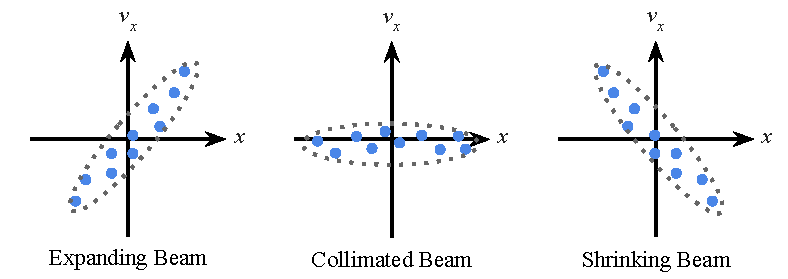
\includegraphics{part2/Figs/EmittanceExample.pdf}
\caption{An example of the trace-space occupied by an expanding, collimated and shrinking beam. The dotted line indicates the area occupied by the beam, the emittance.}
\label{figure:emittance_example}
\end{figure}

The \emph{\gls{rms} emittance} is a more practical measure and is defined as
\begin{equation}\label{emittance}
\bar{\epsilon}_x \equiv \sqrt{\langle x^2\rangle \langle x^{\prime 2}\rangle - \langle x x^\prime\rangle^2}.
\end{equation}

The emittance of a beam represents the `focusability' of the beam.
A low emittance beam can be focused to a smaller waist than a high emittance beam, in fact a beam with zero emittance could be focused to a point whereas any beam with non-zero emittance has a finite spot size, this is shown in Figure~\ref{figure:focusability}.
This makes emittance an important quantity to consider in almost all beam applications but is particularly important to charged beams due to complications produced by space-charge repulsion.

\begin{figure}
\center
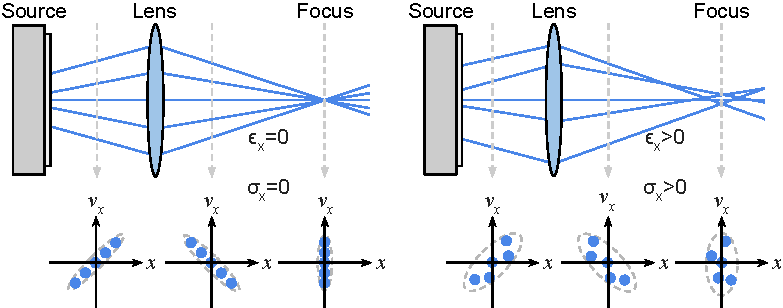
\includegraphics{part2/Figs/EmittanceFocasability.pdf}
\caption{On the left is a particle beam with zero emittance, and thus can be focused to a beam waist of zero width. On the right is a beam with non-zero emittance and thus a non-zero beam waist. Below each figure are plots of the phase space at difference points in the beam where the dashed line is indicative of the phase-space area or emittance.}
\label{figure:focusability}
\end{figure}

The emittance of a beam is not the only factor that determines the quality of the beam.
Emittance could be made arbitrarily small through the use of collimating slits however the reduced particle could would reduce the usefulness of that beam for most applications.
A more comprehensive figure of merit is the number of particles with a given emittance, known as \emph{brightness}~\cite{reiser_theory_2008};
\begin{equation}
B = \frac{I}{8\pi^2\bar{\epsilon}_x\bar{\epsilon}_y},
\end{equation}
where $I$ is the current of the beam and $\bar{\epsilon}_{x,y}$ is the \gls{rms} emittance as described above.
Brightness provides a better metric of a beam's quality with the additional requirement of knowing the beam current.

When comparing the emittance and brightness of particle beams from different sources it is often useful to use the \emph{normalised} emittance and brightness
\begin{align}
\bar{\epsilon}_{n,x} = \beta\bar{\epsilon}_x,\\
B_n = \frac{I}{8\pi^2\bar{\epsilon}_{n,x}\bar{\epsilon}_{n,y}}
\end{align}
where $\beta=v/c\approx v_z/c$.


\subsection{Emittance with a CAEIS}
\label{section:excess_energy_emittance}

For a \gls{caes} the normalised \gls{rms} emittance at the source is given by~\cite{mcculloch_high-coherence_2013}
\begin{equation}\label{equation:excess_energy_emittance}
\bar{\epsilon}_{n,x} = \sigma_x \sqrt{\frac{k_B T}{m c^2}}
\end{equation}
where $\sigma_x$ is the \gls{rms} beam radius, $k_B$ is Boltzmann's constant, $T$ is the temperature of the source, $m$ is the particle mass and $c$ is the speed of light.
Equation~\ref{equation:excess_energy_emittance} highlights one of the advantages of a \gls{caeis} as the low source temperature allows for low emittance bunches compared to the common thermionic sources.

The temperature of the \gls{caeis} source can be calculated from the wavelength of the ionisation lasers, $\lambda_{red}$ and $\lambda_{blue}$,
\begin{align}
 E_{red} &= \frac{hc}{\lambda_{red}} \\
 E_{blue}&= \frac{hc}{\lambda_{blue}},
\end{align}
where $h$ is Plank's constant.
We can define the total ionisation energy to be
\begin{align}
E_{total} = E_{red} + E_{blue}.
\end{align}
The ionisation energy for Rubidium 85, $E_I$ is \unit[4.18]{eV} so we can determine the excess energy of ionisation
\begin{equation}
E_{excess} = E_{total} - E_I
\end{equation}

The excess energy can be related to the temperatures of the ionised particles via
\begin{equation}\label{equation:excess_energy_temperature}
T = \frac{E_{excess}}{k_B}.
\end{equation}
Combining Equations \ref{equation:excess_energy_emittance} and \ref{equation:excess_energy_temperature} allows for the calculation of the expected emittance of bunches generated from the \gls{caeis} for above-threshold ionisation.
The emittance of bunches generated from below-threshold pathways, such as Rydberg-excitation with field-ionisation, cannot be calculated using Equation~\ref{equation:excess_energy_emittance}.

\section{Measurement}

Directly calculating the emittance of an ensemble with Equation~\ref{emittance} requires full knowledge of the position and momenta of the particles which is difficult as beam monitors tend to only measure the transverse positions of particles.
There are a number of methods to practically calculate the emittance of a particle beam, namely pepperpots, the multiple profile method methods and the quadrupole method.
In the \gls{caeis} the quadrupole method is not practical as the lenses in the system are not well characterised and multi-profile measurements are tedious due to the manual z-translation of the detector and bellows.
The pepperpot method however is eminently achievable with this system although the details of the geometry are not ideal with this iteration of a \gls{caeis}.

\subsection{Pepperpots}

The pepperpot method uses a beam mask, consisting of an array of small holes, to separate the beam into a number of `beamlets' which are then propagated and detected downstream.
By examining the size of the beamlets the divergence of the beam can be estimated and thus the emittance of the beam can be calculated.
Ideally the extent of the array should be larger than the size of the beam and the holes are as small as is practical while maintaining sufficient flux and ensuring the spots on the detector do not overlap.
The name refers to the similarity of the simplest beam mask to the perforated lid of a container for pepper.

A useful derivation of this technique is presented in Ref.~\cite{zhang_emittance_1996} with the one dimensional result:

\begin{dmath}\label{equation:pepperpot}
\epsilon_x^2 = \left\langle x^2\right\rangle \left\langle x^{\prime2}\right\rangle - \left\langle xx^\prime\right\rangle^2\allowbreak
\approx \frac{1}{N^2} \left\{\left[\sum_{j=1}^p{n_j\left(x_{sj}-\bar{x}\right)^2}\right] \left[ \sum_{j=1}^p{\left[n_j\sigma_{x_j^\prime}^2 + n_j\left(\bar{x_j^\prime}-\bar{x^\prime}\right)^2\right]}\right] - \left[ \sum_{j=1}^p{n_jx_{sj}\bar{x_j^\prime}-N\bar{x}\bar{x^\prime}}\right]^2\right\}
\end{dmath}
where;
\begin{itemize}
    \item $N$ is the total number of particles after the beam mask,
    \item $p$ is the total number of holes in the $x$ direction,
    \item $n_j$ is the number of particles passing through the $j$-th hole and hitting the detector,
    \item $x_{sj}$ is position of the $j$-th hole,
    \item $\bar{x}$ is the mean position of the holes,
    \item $\sigma_{x_j^\prime}$ is the \gls{rms} divergence of the $j$-th beamlet,
    \item $\bar{x_j^\prime}$ is the mean divergence of the $j$-th beamlet, and
    \item $\bar{x^\prime}$ is the mean divergence of all beamlets.
\end{itemize}

An example pepperpot mask and detected beamlets are shown in Figure~\ref{figure:pepperpot_example}.
This equation can be implemented by appropriately rotating the detected beamlets and then performing row and column sums of the pixels followed by application of Equation~\ref{equation:pepperpot} for $x$ and $y$.

\begin{figure}
    \centering
    \begin{subfigure}{0.49\linewidth}
    \centering
    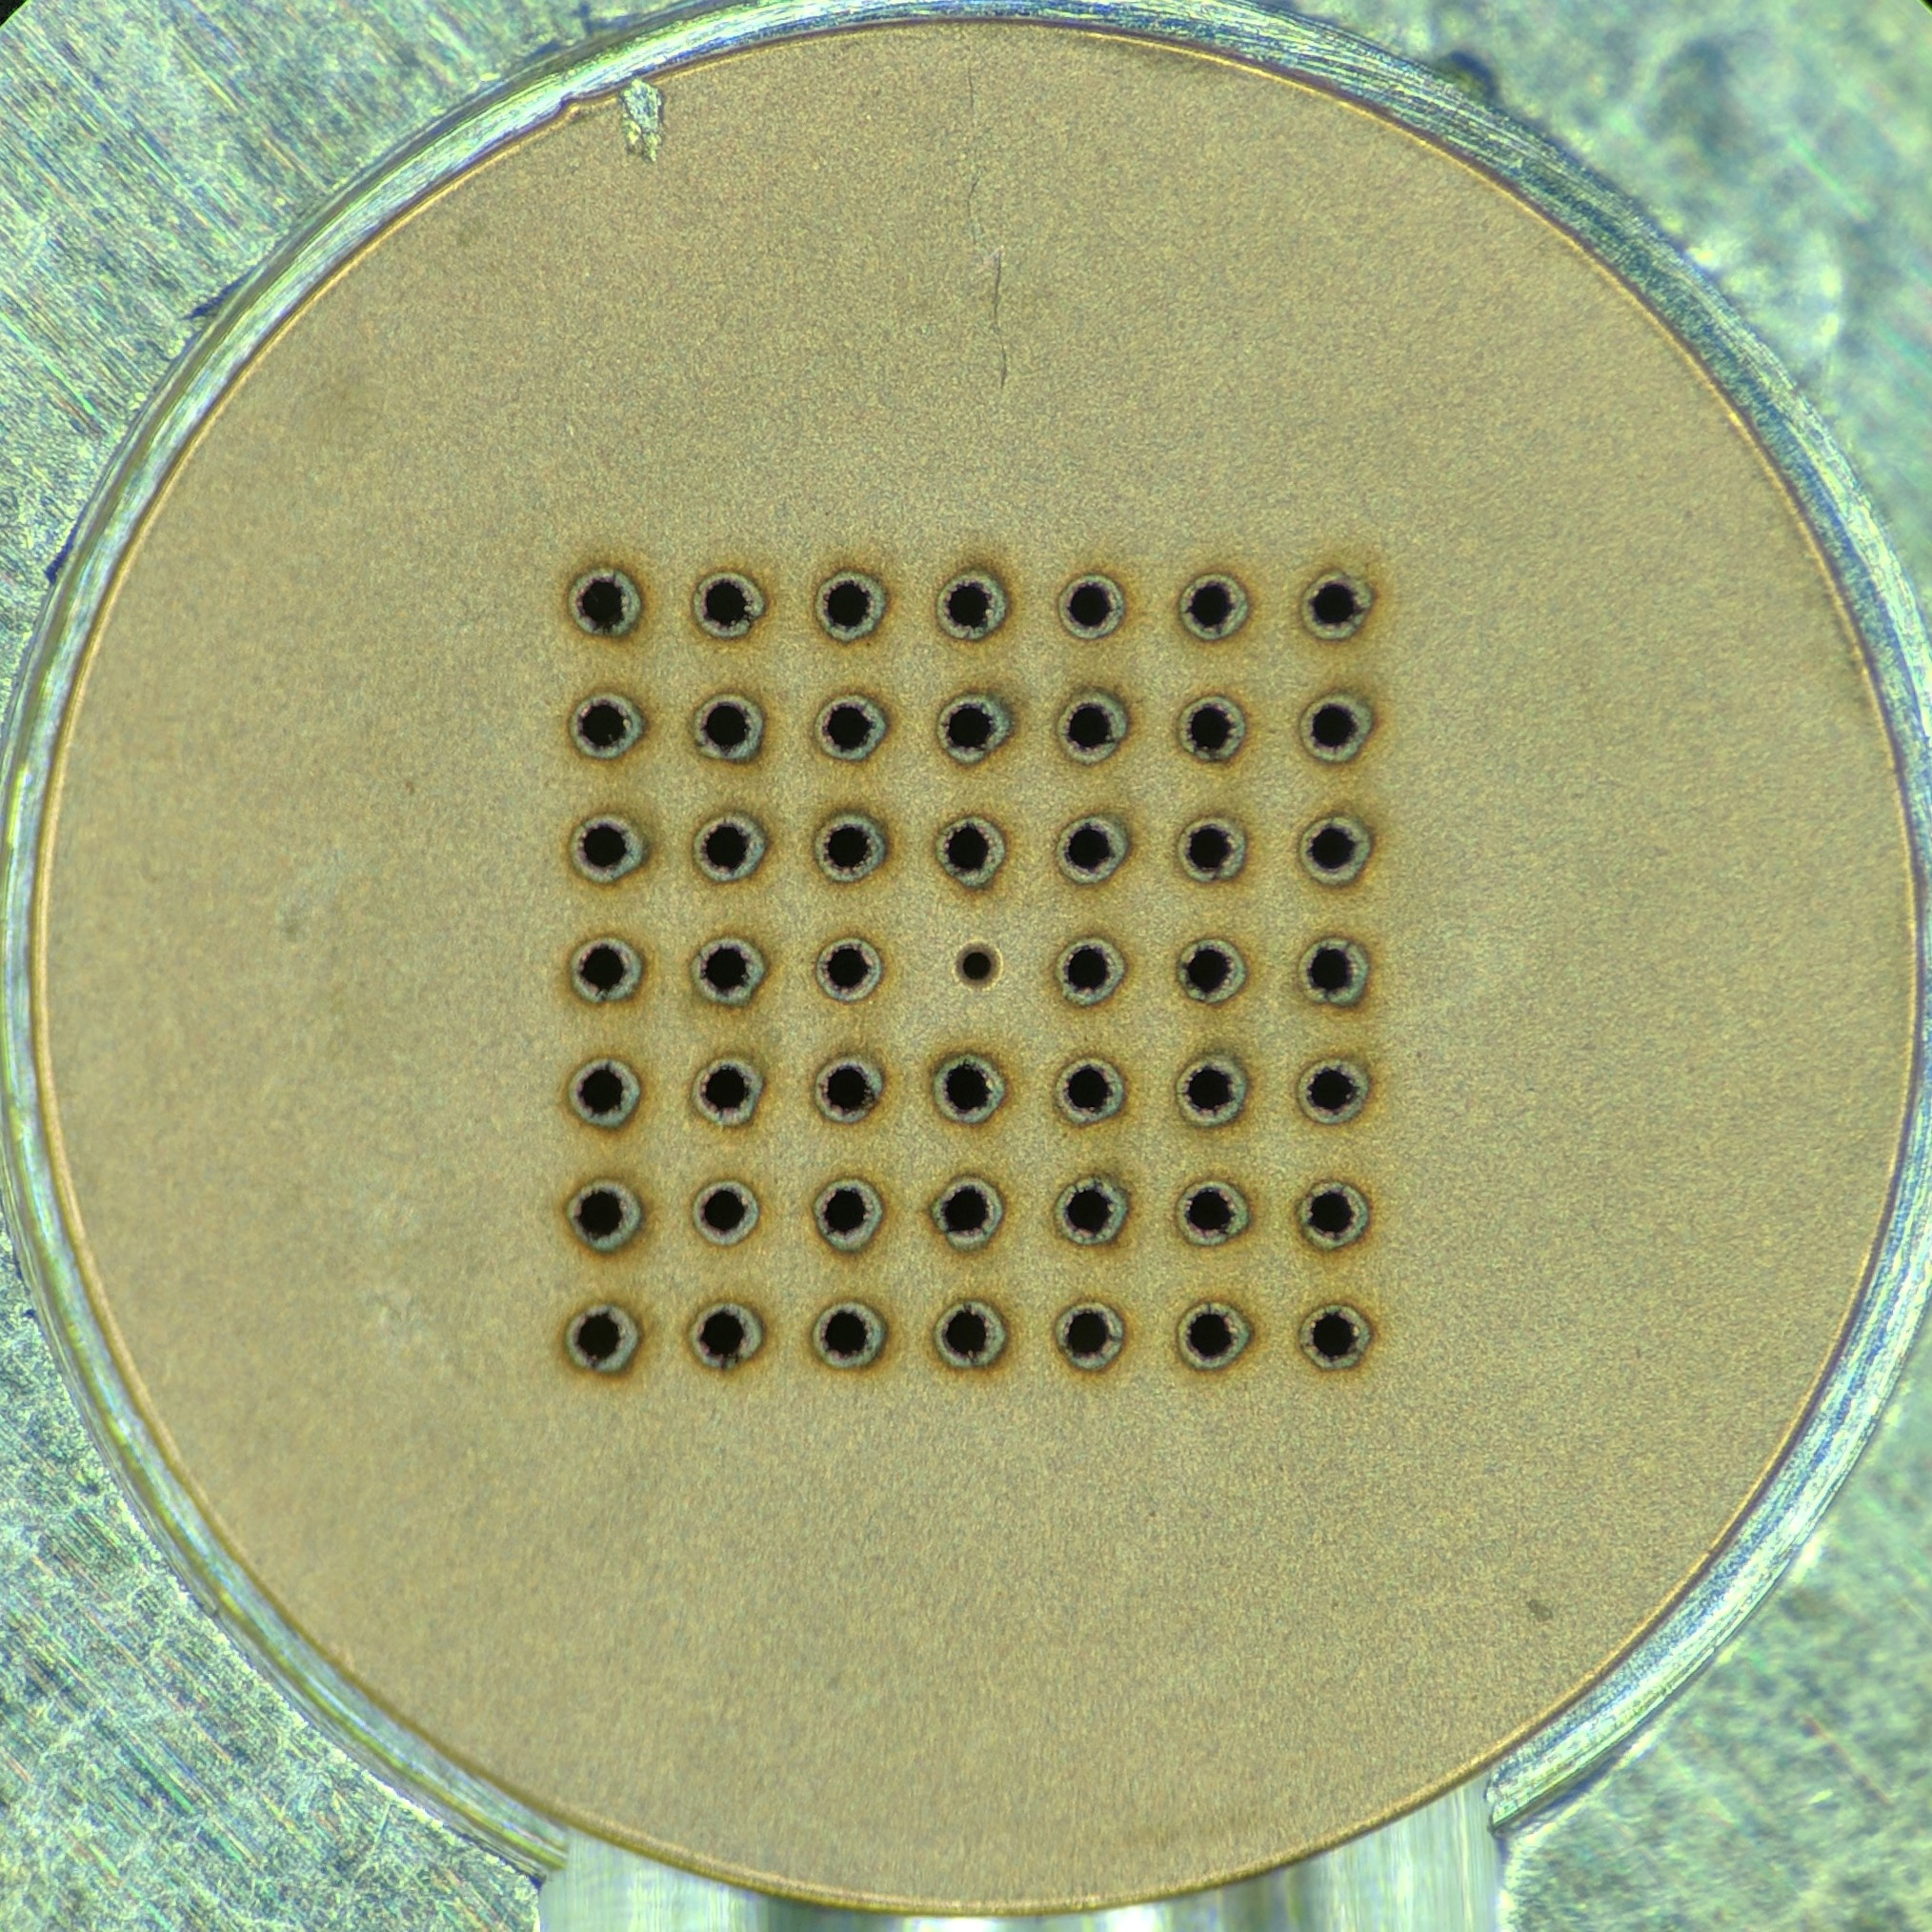
\includegraphics[width=\linewidth]{part2/Figs/example_pepperpot_mask.jpg}
    \caption{}
    \label{figure:pepperpot_mask}
    \end{subfigure}
    \begin{subfigure}{0.49\linewidth}
    \centering
    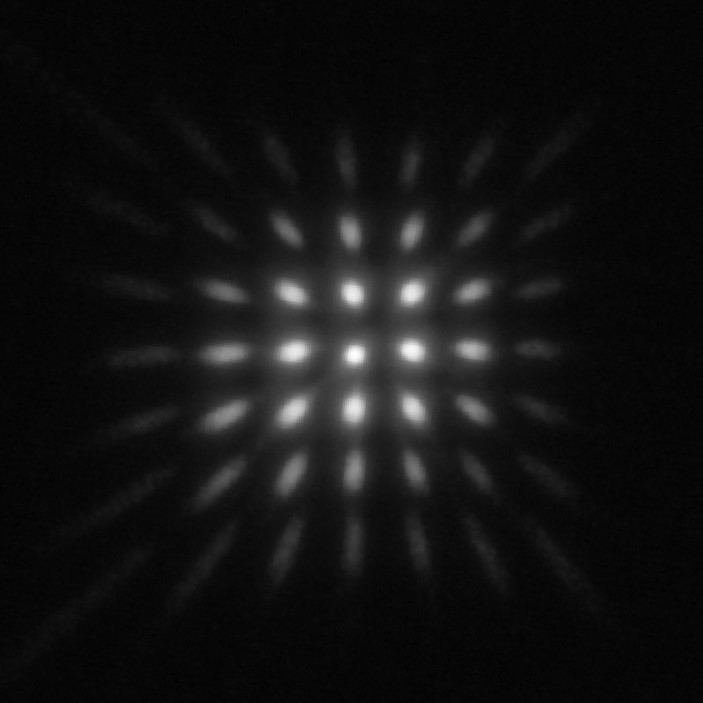
\includegraphics[width=\linewidth]{part2/Figs/example_pepperpot_detector_linear.jpeg}
    % 486.971 pepperpot from 2017.06.06
    \caption{}
    \label{figure:pepperpot_image}
    \end{subfigure}
    
    \begin{subfigure}{0.49\linewidth}
    \centering
    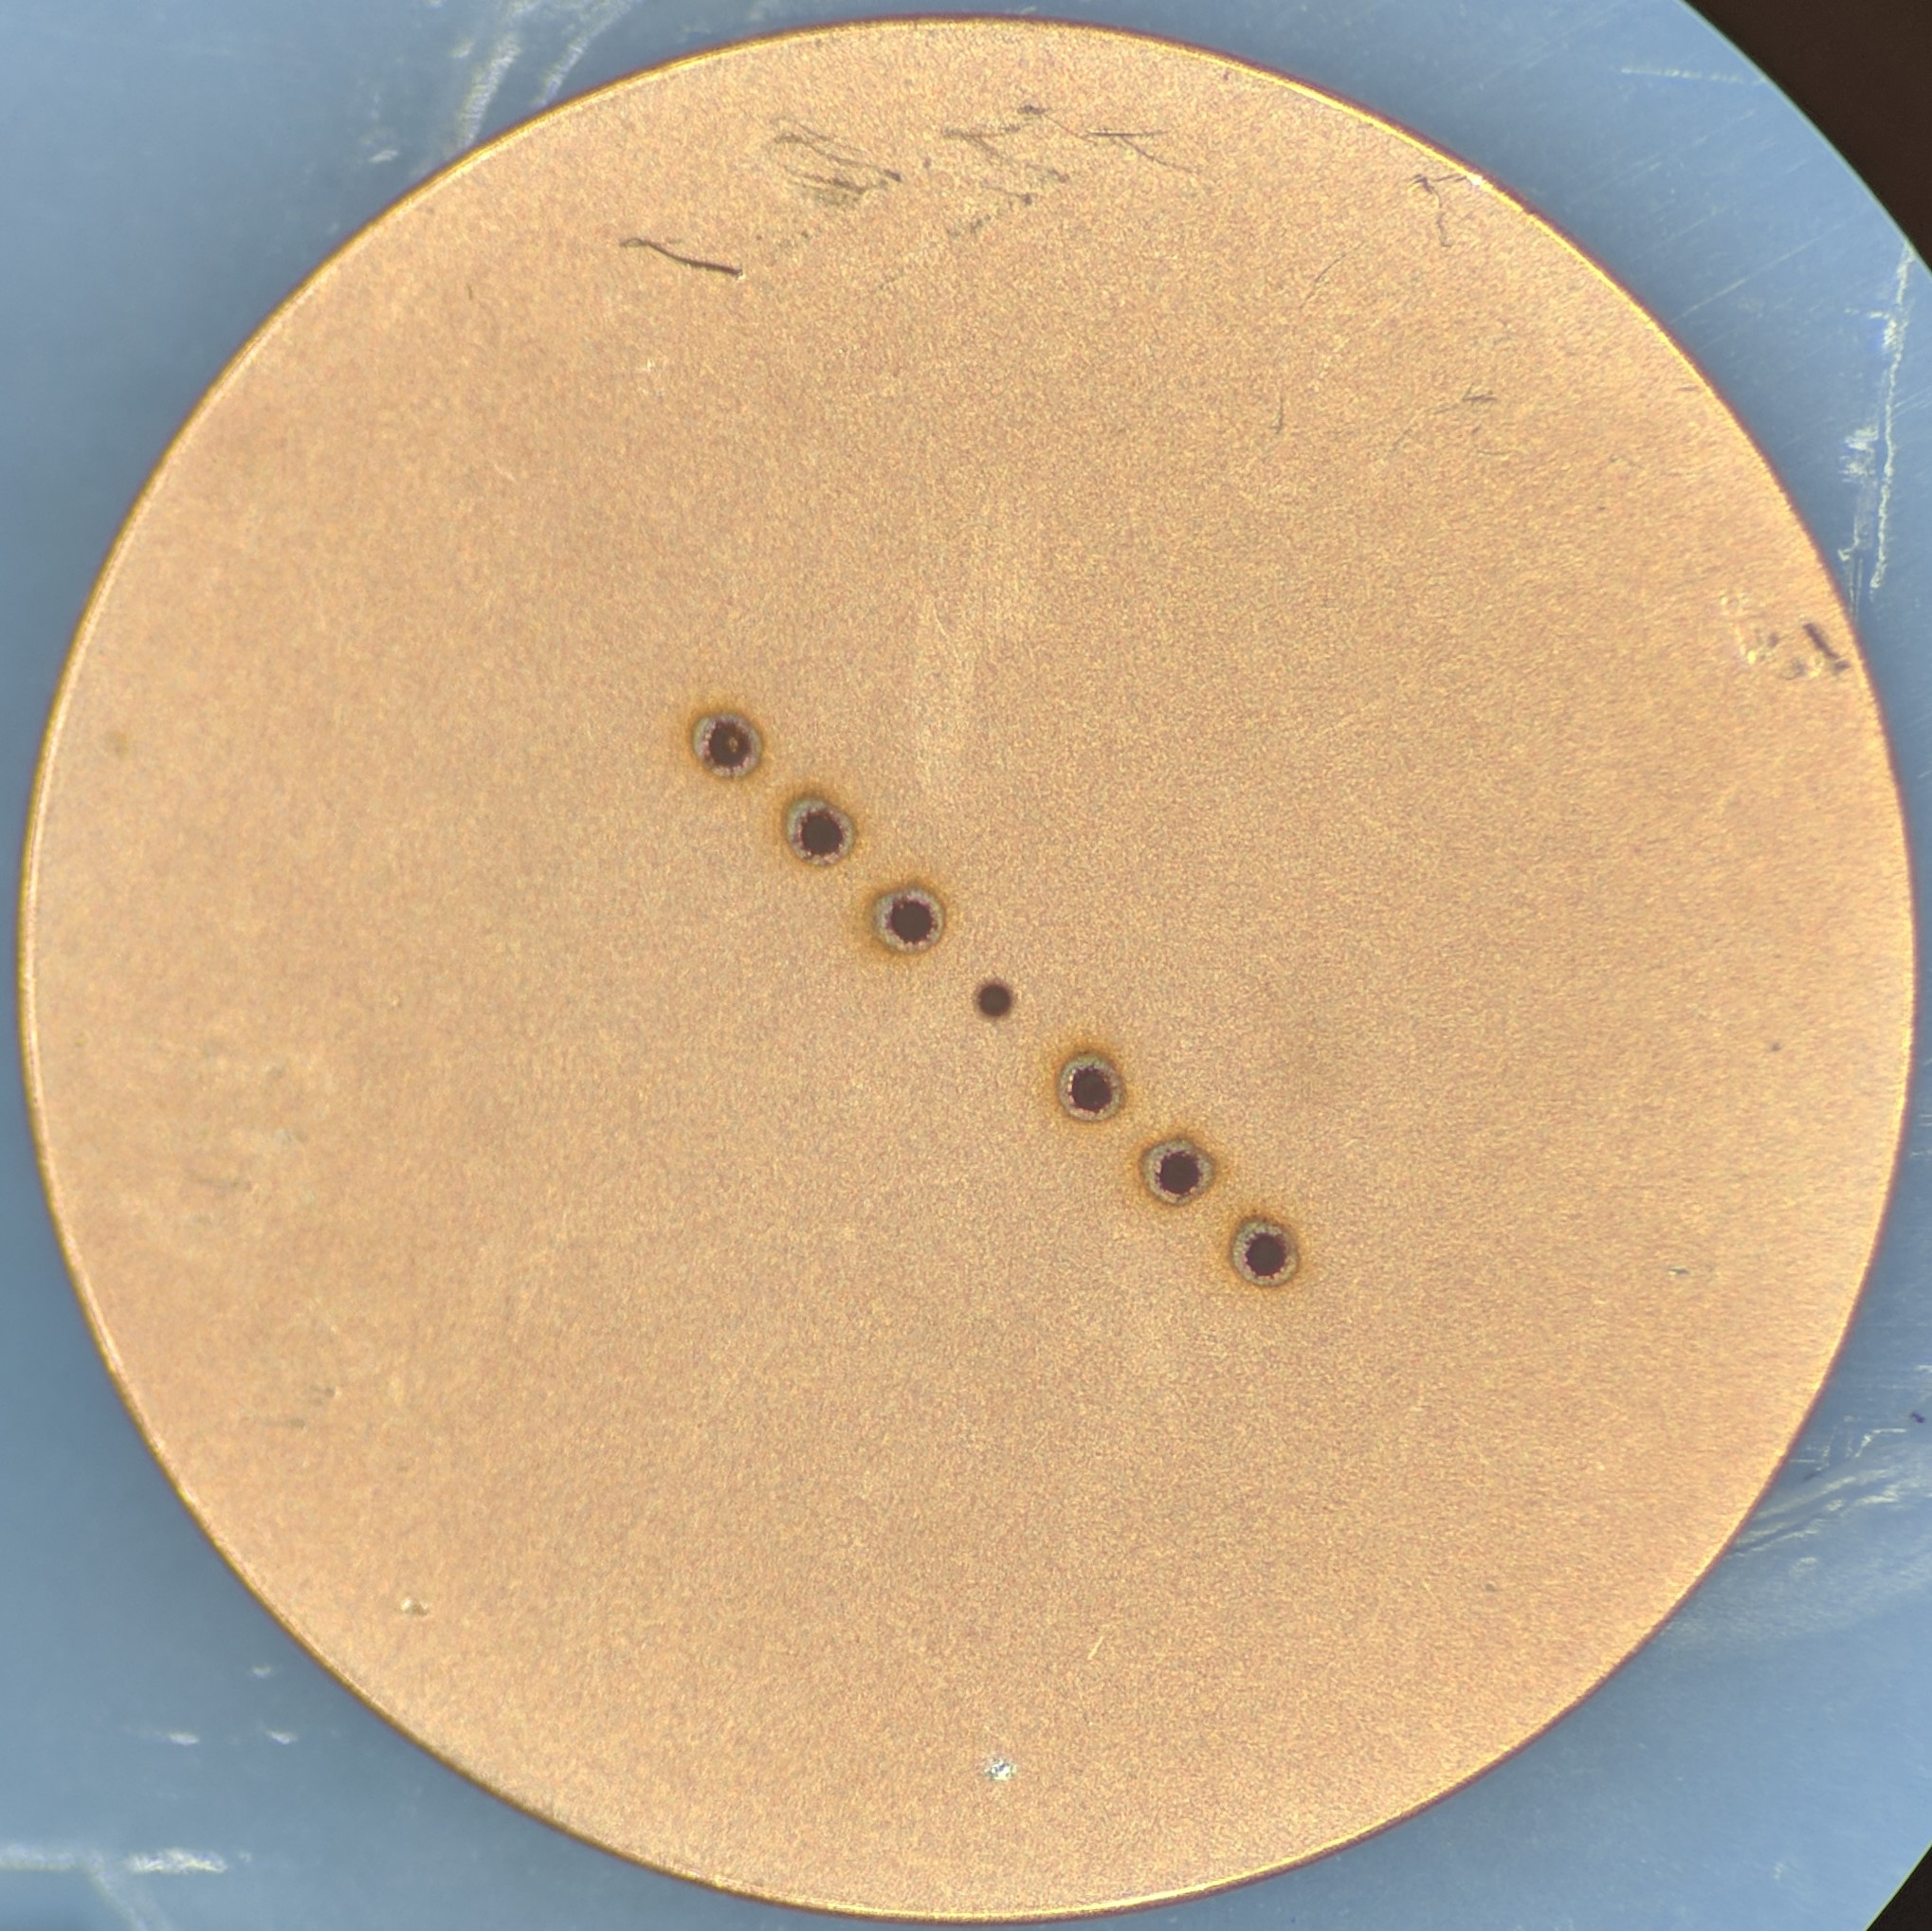
\includegraphics[width=\linewidth]{part2/Figs/example_pepperpot_1d.jpg}
    \caption{}
    \label{figure:1d_pepperpot}
    \end{subfigure}
    \begin{subfigure}{0.49\linewidth}
    \centering
    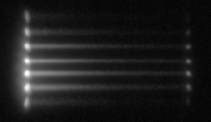
\includegraphics[width=\linewidth]{part2/Figs/example_streaked_pepperpot.png}
    \caption{}
    \label{figure:streaked_1d_pepperpot}
    \end{subfigure}
    % Manual labels.....
    \caption{(a) a pepperpot mask cut into a thing copper disk and, (b), the corresponding set of beamlets on the detector. (c) a one-dimensional pepperpot mask (held in place by a copper ring) and the corresponding streaked set of beamlets on the detector, (d). The beam images are log scaled.}
    \label{figure:pepperpot_example}
\end{figure}

\subsubsection{Temporal Resolution with Streaking}
A one-dimensional pepperpots can consist of a line of apertures and provides a prime target for a streak measurements.
In this case streaking is performed with a time varying electric field which deflects the charged particles across the detector, providing time-resolution.
For a pulsed charged particle source, such as the \gls{caeis}, the streak can be performed over the duration of the bunch or over a portion of the bunch if higher resolution is required.
There are some considerations for how fast an electric field can be swept, which will not be examined in detail here, so extremely short bunches will require more complicated systems, such as a \gls{rf} cavity or photoactivated switching, to provide the appropriate timing and electric field temporal-gradient~\cite{alesini_rf_2006,kassier_compact_2010}.
An example of a streaked pepperpot measurement is shown in Figure~\ref{figure:streaked_1d_pepperpot}.

% \subsection{Multi-profile Method}

% If a beam can be described by $\sigma^0$ at $z_0$ and by $\sigma^1$ at $z_1$ then the transformation matrix, $\mathbf{R}_{12}$ from $z_0$ to $z_1$ is
% \begin{equation}
% \mathbf{R} = \begin{pmatrix} R_{11} & R_{12} \\ R_{21} & R_{22} \end{pmatrix}
% \end{equation}
% and
% \begin{equation}
% \sigma^1 = \mathbf{R}\sigma^0\mathbf{R}^T
% \end{equation}
% where $\mathbf{R}^T$ is the transpose of $\mathbf{R}$.
% The combined transfer matrix for a series of $z$ positions is simply the product of the individual transfer matrices.

% We can write:
% \begin{equation}\label{equation:multiprofile}
% \sigma_{11}^1 = R_{11}^2\sigma_{11}^0 + 2R_{11}R_{12}\sigma_{12}^0 + R_{12}^2\sigma_{22}^0
% \end{equation}

% Typical detectors are only able to measure the standard deviation of $x$, $\sigma_{11}$.
% With at least three measurements and known transfer matrices the other elements of $\sigma$ can be determined.
% With more than three measurements uncertainty can be reduced.

% The transfer matrix for simple propagation over a distance $L$ is
% \begin{equation}
% \mathbf{R}_L = \begin{pmatrix}1 & L \\ 0 & 1\end{pmatrix}
% \end{equation}
% and then Equation~\ref{equation:multiprofile} becomes
% \begin{equation}
% \sigma_{11}^1 = \sigma_{11}^0 + 2L \sigma_{12}^0 + L_1^2\sigma_{22}^0.
% \end{equation}

% \begin{figure}
% \center
% 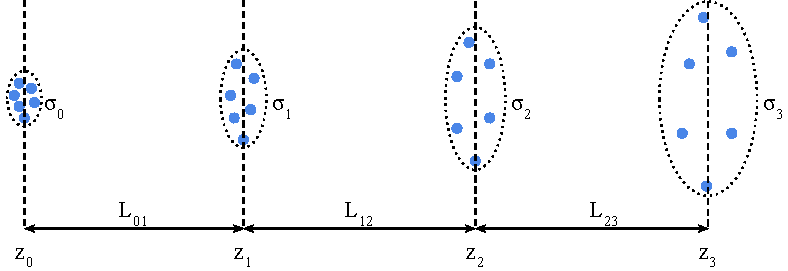
\includegraphics{part2/Figs/Multi-ProfileEmittance.pdf}
% \caption{An example of a multi-profile emittance measurement conducted on an expanding beam travelling from left to right (or a shrinking beam travelling right to left).}
% \label{figure:multiprofileexample}
% \end{figure}

% With an initial beam, $\sigma_0$, measured at $z_1, z_2$ and $z_3$ as shown in Figure~\ref{figure:multiprofileexample} then $\sigma_{11}^1$, $\sigma_{11}^2$, and $\sigma_{11}^3$ are know and we can write 
% \begin{align}
% \sigma_{11}^1 &= \sigma_{11}^0 +2L_{01}\sigma_{12}^0 + L_{01}^2\sigma_{22}^0 \notag\\
% \sigma_{11}^2&= \sigma_{11}^0+2(L_{01}+L_{12})\sigma_{12}^0 + (L_{01}+L_{12})^2\sigma_{22}^0 \notag\\
% \sigma_{11}^3&= \sigma_{11}^0+2(L_{01}+L_{12}+L_{23})\sigma_{12}^0 + (L_{01}+L_{12}+L_{23})^2\sigma_{22}^0 \label{eq:multiprofilesolution}
% \end{align}

% Which can easily be solved for $\sigma_0$ thus allowing the calculation of the emittance with Equation~\ref{eq:emittancewithdeterminant}.

% This method is feasible with the \gls{caeis} at the University of Melbourne but labourious due to the manual operation of the bellows the detector is attached to.

% \subsection{Quadrupole Method}

% The quadrupole method is similar to the multi-profile method but requires only a single location to measure the beam width and a well characterised variable lens such as a quadrupole lens.
% A quadrupole lens with a magnetic field gradient of $G$ has the transfer matrix in the focusing plane of
% \begin{equation}
% \mathbf{R}_f = \begin{pmatrix} \cos kl & (1/k)\sin kl\\
% -k\sin kl & cos kl\end{pmatrix},
% \end{equation}
% where $l$ is the effective length of the quadrupole, $k^2=G/B\rho$ is the quadrupole strength and $B\rho$ is the magnetic rigidity of the particles in the assumed central trajectory.
% The matrix in the defocusing plane is
% \begin{equation}
% \mathbf{R}_d = \begin{pmatrix} \cosh kl & (1/k) \sin kl\\
% k \sinh kl & \cosh kl \end{pmatrix}
% \end{equation}

% A beam measured a distance $L$ away from the quadrupole will have undergone the transformation $\mathbf{R}=\mathbf{R}_L\mathbf{R}_f$ on one axis and $\mathbf{R}=\mathbf{R}_L\mathbf{R}_d$ on the other.
% The symmetric beam matrix for the beam before the lens can then be determined from a series of beam profile measurements with different focusing strengths.
% The main advantage of this measurement is that is only requires a single beam monitor location.

% Due to the ad hoc nature of the magnetic lenses used in the \gls{caes} this method is not practical without a thorough characterisation of the lenses, especially in comparison with the ease of the alternative methods.

\section{Experimental Setup}

A number of modifications were made to the \gls{caeis} to prepare it for the streaked emittance measurements and there were a number of restrictions on various parameters due to the precise setup of the apparatus.
The \gls{caeis} was operated in electron mode for these measurements due to the available magnetic optics and the larger emittance expected from electrons as the source temperature is higher for electrons, a minimum temperature of approximately \unit[10]{K} for electrons and \unit[100]{$\muup K$} for ions~\cite{saliba_spatial_2012}.
Using electrons also allows some control of the bunch emittance as the excess energy can be controlled with the blue ionisation laser wavelength, with ions the change in emittance would be negligible.

See Chapter~\ref{chapter:setup} for a more detailed description of the \gls{caeis} and Figure~\ref{figure:emittance_schematic} for a schematic of the setup used for the measurements in this chapter.

\begin{figure}
\center
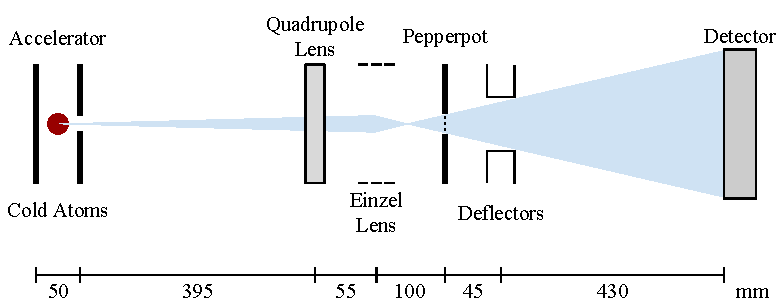
\includegraphics{part2/Figs/EmittanceApparatusSchematic.pdf}
\caption{A schematic of the experimental apparatus with relevant dimensions. The blue region indicates the electron beam envelope. Note that components are not necessarily orientate realistically in this schematic (particularly the deflectors).}
\label{figure:emittance_schematic}
\end{figure}

\subsection{Beam Optics}
The quadrupole electron optics discussed in Section \ref{section:quadrupole} were use to reduce the astigmatism present in the electron beam as discussed in the aforementioned section.
The two-dimensional pepperpot provide another avenue to monitor the astigmatism of the beam as with an astigmatic beam the spacing of the beamlets on the detector are not the same along each axis as shown in Figure~\ref{figure:astigmatic_pepperpot}.
When focussing was required the Einzel lens was used.

\begin{figure}
    \center
    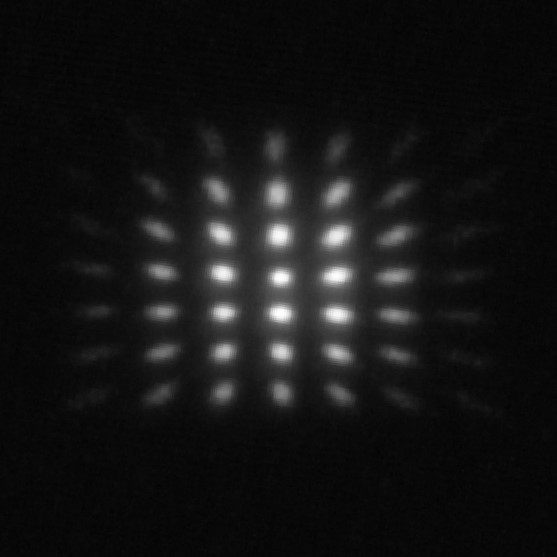
\includegraphics[width=0.5\linewidth]{part2/Figs/example_astigmatic_pepperpot.jpeg}
    \caption{An example of a pepperpot without the beam correction from the quadrupole lens. It is readily apparent that spacing of the beamlets is not the same for the $x$ and $y$ axes. This image is log scaled.}
    \label{figure:astigmatic_pepperpot}
    % From 2017.06.01
\end{figure}

A number of permanent magnets were used to steer the beam through the various apertures and onto the detector and care was taken to attempt to keep the beam on the central axis of the apparatus.
This was achieved by manually adjusting the positions of the magnets, which were mounted on posts external to the vacuum system, to ensure that the beam was passing through the apertures in the system and by scanning the Einzel lens to verify that the beam was passing through its centre.
Due to the unstable nature of the apparatus these magnets needed to be adjusted on a day-to-day basis to maintain the beam path.

The main limiting factor to pepperpot emittance measurements using the \gls{caes} was electron flux through the pepperpot masks.
Flux through the pepperpot masks was maximised by using the Einzel lens to focus the beam to the approximate size of the pepperpots in the pepperpot plane, thus maximising the flux through the apertures.
The Einzel lens voltage required for this was approximately \unit[4.8][kV] and varied slightly beam emittance, i.e.. high emittance beams result in a larger beam size and thus required adjusting the Einzel lens voltage by \unit[100]{V} or so.

\subsection{Beam Energy}
In many emittance measurements the beam energy would not be a free parameter as it will be used as a diagnostic for a specific system or scenario, however in this experiment we are able to vary the energy of our beam from a few hundred eV to around \unit[10]{keV}.
There are a number of considerations in determining the optimal beam energy to use for pepperpot measurements such as measurement resolution, beam current and beam stability.

The resolution of a pepperpot measurement is greater when the size of the beamlets on the detector is larger and, as shown in Equation~\ref{equation:divergence} the divergence is greater for slower beams.
Unfortunately the slower the beam the more fragile the alignment of the beam becomes.
While attempting to align a \unit[500][eV] beam through it system it was impossible to position the steering magnets such that an unobstructed beam made it through the system to the detector.

A relatively high energy beam of \unit[8]{keV} was used as this provided a robust beam alignment that was resistant to the transient changes in the magnetic environment while providing sufficient measurement resolution.

\subsection{Bellows}

The bellows provide an additional mechanism to control the resolution of the measurement by adjusting the propagation distance of the pepperpot beamlets and thus their size on the detector.
As this parameter is also adjustable with the strength of the Einzel lens the bellows were placed approximately halfway between the minimum and maximum position where the beam alignment was still well behaved.

{\color{red}Add photo of bellows}

\subsection{Streaking}
The streaking was performed using a pair of deflectors located after the pepperpot sample and orientated such that the one-dimensional pepperpots could be streaked across the detector.
For these measurements one deflector was grounded and the other given a time-varying voltage which was supplied in one of two ways:
\begin{itemize}
\item A fast ramp using a bipolar push-pull solid-state switch with a fixed transition time of \unit[10]{ns} and
\item A slower ramp using an amplified signal generator with a minimum transition of approximately \unit[10]{$\muup$s}.
\end{itemize}
An example of the voltage ramps is shown in Figure~\ref{figure:deflector_voltages}. The slow ramp was done by amplifying the output of signal generator\footnote{Rigol DG4162, able to operate up to \unit[160]{MHz}} which is highly configurable and thus capable of a wide range of pulse lengths, limited by the speed of the amplifier to a transition time approximately \unit[10]{$\muup$s} in duration as shown in Figure~\ref{figure:deflector_voltages}.
More detail on the design of the streaking electronics can be found in Reference~{\color{red}(Cite Rory's thesis)}.

\begin{figure}
    \center
    %% Creator: Matplotlib, PGF backend
%%
%% To include the figure in your LaTeX document, write
%%   \input{<filename>.pgf}
%%
%% Make sure the required packages are loaded in your preamble
%%   \usepackage{pgf}
%%
%% Figures using additional raster images can only be included by \input if
%% they are in the same directory as the main LaTeX file. For loading figures
%% from other directories you can use the `import` package
%%   \usepackage{import}
%% and then include the figures with
%%   \import{<path to file>}{<filename>.pgf}
%%
%% Matplotlib used the following preamble
%%
\begingroup%
\makeatletter%
\begin{pgfpicture}%
\pgfpathrectangle{\pgfpointorigin}{\pgfqpoint{5.710000in}{1.903333in}}%
\pgfusepath{use as bounding box, clip}%
\begin{pgfscope}%
\pgfsetbuttcap%
\pgfsetmiterjoin%
\definecolor{currentfill}{rgb}{1.000000,1.000000,1.000000}%
\pgfsetfillcolor{currentfill}%
\pgfsetlinewidth{0.000000pt}%
\definecolor{currentstroke}{rgb}{1.000000,1.000000,1.000000}%
\pgfsetstrokecolor{currentstroke}%
\pgfsetdash{}{0pt}%
\pgfpathmoveto{\pgfqpoint{0.000000in}{0.000000in}}%
\pgfpathlineto{\pgfqpoint{5.710000in}{0.000000in}}%
\pgfpathlineto{\pgfqpoint{5.710000in}{1.903333in}}%
\pgfpathlineto{\pgfqpoint{0.000000in}{1.903333in}}%
\pgfpathclose%
\pgfusepath{fill}%
\end{pgfscope}%
\begin{pgfscope}%
\pgfsetbuttcap%
\pgfsetmiterjoin%
\definecolor{currentfill}{rgb}{1.000000,1.000000,1.000000}%
\pgfsetfillcolor{currentfill}%
\pgfsetlinewidth{0.000000pt}%
\definecolor{currentstroke}{rgb}{0.000000,0.000000,0.000000}%
\pgfsetstrokecolor{currentstroke}%
\pgfsetstrokeopacity{0.000000}%
\pgfsetdash{}{0pt}%
\pgfpathmoveto{\pgfqpoint{0.661914in}{0.570703in}}%
\pgfpathlineto{\pgfqpoint{3.110957in}{0.570703in}}%
\pgfpathlineto{\pgfqpoint{3.110957in}{1.753333in}}%
\pgfpathlineto{\pgfqpoint{0.661914in}{1.753333in}}%
\pgfpathclose%
\pgfusepath{fill}%
\end{pgfscope}%
\begin{pgfscope}%
\pgfpathrectangle{\pgfqpoint{0.661914in}{0.570703in}}{\pgfqpoint{2.449043in}{1.182630in}} %
\pgfusepath{clip}%
\pgfsetrectcap%
\pgfsetroundjoin%
\pgfsetlinewidth{1.003750pt}%
\definecolor{currentstroke}{rgb}{0.309804,0.478431,0.682353}%
\pgfsetstrokecolor{currentstroke}%
\pgfsetdash{}{0pt}%
\pgfpathmoveto{\pgfqpoint{0.661914in}{0.639863in}}%
\pgfpathlineto{\pgfqpoint{0.685907in}{0.638678in}}%
\pgfpathlineto{\pgfqpoint{0.688437in}{0.638833in}}%
\pgfpathlineto{\pgfqpoint{0.691552in}{0.639256in}}%
\pgfpathlineto{\pgfqpoint{0.710846in}{0.640263in}}%
\pgfpathlineto{\pgfqpoint{0.712757in}{0.639892in}}%
\pgfpathlineto{\pgfqpoint{0.716371in}{0.638523in}}%
\pgfpathlineto{\pgfqpoint{0.720898in}{0.639289in}}%
\pgfpathlineto{\pgfqpoint{0.723118in}{0.639239in}}%
\pgfpathlineto{\pgfqpoint{0.725751in}{0.638742in}}%
\pgfpathlineto{\pgfqpoint{0.730157in}{0.640450in}}%
\pgfpathlineto{\pgfqpoint{0.733238in}{0.640418in}}%
\pgfpathlineto{\pgfqpoint{0.735820in}{0.640113in}}%
\pgfpathlineto{\pgfqpoint{0.741534in}{0.638183in}}%
\pgfpathlineto{\pgfqpoint{0.743806in}{0.638528in}}%
\pgfpathlineto{\pgfqpoint{0.747042in}{0.639045in}}%
\pgfpathlineto{\pgfqpoint{0.752498in}{0.639197in}}%
\pgfpathlineto{\pgfqpoint{0.756921in}{0.640379in}}%
\pgfpathlineto{\pgfqpoint{0.760088in}{0.639106in}}%
\pgfpathlineto{\pgfqpoint{0.764064in}{0.638800in}}%
\pgfpathlineto{\pgfqpoint{0.769313in}{0.639684in}}%
\pgfpathlineto{\pgfqpoint{0.783805in}{0.639351in}}%
\pgfpathlineto{\pgfqpoint{0.792015in}{0.641048in}}%
\pgfpathlineto{\pgfqpoint{0.796215in}{0.640030in}}%
\pgfpathlineto{\pgfqpoint{0.807867in}{0.639090in}}%
\pgfpathlineto{\pgfqpoint{0.810448in}{0.639002in}}%
\pgfpathlineto{\pgfqpoint{0.816782in}{0.640631in}}%
\pgfpathlineto{\pgfqpoint{0.819278in}{0.639510in}}%
\pgfpathlineto{\pgfqpoint{0.821636in}{0.639273in}}%
\pgfpathlineto{\pgfqpoint{0.824338in}{0.639420in}}%
\pgfpathlineto{\pgfqpoint{0.826989in}{0.638791in}}%
\pgfpathlineto{\pgfqpoint{0.830242in}{0.639425in}}%
\pgfpathlineto{\pgfqpoint{0.836420in}{0.639113in}}%
\pgfpathlineto{\pgfqpoint{0.840482in}{0.638745in}}%
\pgfpathlineto{\pgfqpoint{0.842806in}{0.639399in}}%
\pgfpathlineto{\pgfqpoint{0.845181in}{0.639797in}}%
\pgfpathlineto{\pgfqpoint{0.849123in}{0.639023in}}%
\pgfpathlineto{\pgfqpoint{0.852668in}{0.639534in}}%
\pgfpathlineto{\pgfqpoint{0.857264in}{0.639722in}}%
\pgfpathlineto{\pgfqpoint{0.862427in}{0.640019in}}%
\pgfpathlineto{\pgfqpoint{0.865886in}{0.639236in}}%
\pgfpathlineto{\pgfqpoint{0.871790in}{0.639947in}}%
\pgfpathlineto{\pgfqpoint{0.874303in}{0.639239in}}%
\pgfpathlineto{\pgfqpoint{0.878933in}{0.639722in}}%
\pgfpathlineto{\pgfqpoint{0.886024in}{0.640670in}}%
\pgfpathlineto{\pgfqpoint{0.900481in}{0.665955in}}%
\pgfpathlineto{\pgfqpoint{0.914991in}{0.692189in}}%
\pgfpathlineto{\pgfqpoint{0.984335in}{0.811283in}}%
\pgfpathlineto{\pgfqpoint{0.986934in}{0.815749in}}%
\pgfpathlineto{\pgfqpoint{0.995781in}{0.831818in}}%
\pgfpathlineto{\pgfqpoint{1.009602in}{0.855721in}}%
\pgfpathlineto{\pgfqpoint{1.013491in}{0.861243in}}%
\pgfpathlineto{\pgfqpoint{1.023181in}{0.875697in}}%
\pgfpathlineto{\pgfqpoint{1.031236in}{0.887602in}}%
\pgfpathlineto{\pgfqpoint{1.044506in}{0.905297in}}%
\pgfpathlineto{\pgfqpoint{1.051305in}{0.916597in}}%
\pgfpathlineto{\pgfqpoint{1.099256in}{0.993578in}}%
\pgfpathlineto{\pgfqpoint{1.105572in}{1.002734in}}%
\pgfpathlineto{\pgfqpoint{1.121028in}{1.028128in}}%
\pgfpathlineto{\pgfqpoint{1.134109in}{1.047792in}}%
\pgfpathlineto{\pgfqpoint{1.137121in}{1.053476in}}%
\pgfpathlineto{\pgfqpoint{1.139995in}{1.056965in}}%
\pgfpathlineto{\pgfqpoint{1.142990in}{1.060511in}}%
\pgfpathlineto{\pgfqpoint{1.160460in}{1.089288in}}%
\pgfpathlineto{\pgfqpoint{1.198376in}{1.148417in}}%
\pgfpathlineto{\pgfqpoint{1.201302in}{1.153386in}}%
\pgfpathlineto{\pgfqpoint{1.205037in}{1.159542in}}%
\pgfpathlineto{\pgfqpoint{1.213677in}{1.171255in}}%
\pgfpathlineto{\pgfqpoint{1.220269in}{1.181702in}}%
\pgfpathlineto{\pgfqpoint{1.225588in}{1.189842in}}%
\pgfpathlineto{\pgfqpoint{1.236190in}{1.205469in}}%
\pgfpathlineto{\pgfqpoint{1.272230in}{1.255450in}}%
\pgfpathlineto{\pgfqpoint{1.276172in}{1.260278in}}%
\pgfpathlineto{\pgfqpoint{1.284846in}{1.273493in}}%
\pgfpathlineto{\pgfqpoint{1.301077in}{1.296105in}}%
\pgfpathlineto{\pgfqpoint{1.308288in}{1.305361in}}%
\pgfpathlineto{\pgfqpoint{1.312540in}{1.311632in}}%
\pgfpathlineto{\pgfqpoint{1.318237in}{1.319983in}}%
\pgfpathlineto{\pgfqpoint{1.331334in}{1.337047in}}%
\pgfpathlineto{\pgfqpoint{1.340715in}{1.348001in}}%
\pgfpathlineto{\pgfqpoint{1.360336in}{1.368650in}}%
\pgfpathlineto{\pgfqpoint{1.367186in}{1.371538in}}%
\pgfpathlineto{\pgfqpoint{1.369974in}{1.371728in}}%
\pgfpathlineto{\pgfqpoint{1.378580in}{1.372520in}}%
\pgfpathlineto{\pgfqpoint{1.382383in}{1.373033in}}%
\pgfpathlineto{\pgfqpoint{1.385671in}{1.372624in}}%
\pgfpathlineto{\pgfqpoint{1.391798in}{1.369904in}}%
\pgfpathlineto{\pgfqpoint{1.398751in}{1.367030in}}%
\pgfpathlineto{\pgfqpoint{1.401936in}{1.366306in}}%
\pgfpathlineto{\pgfqpoint{1.405051in}{1.365280in}}%
\pgfpathlineto{\pgfqpoint{1.412916in}{1.361527in}}%
\pgfpathlineto{\pgfqpoint{1.414620in}{1.360642in}}%
\pgfpathlineto{\pgfqpoint{1.418803in}{1.357469in}}%
\pgfpathlineto{\pgfqpoint{1.422830in}{1.356282in}}%
\pgfpathlineto{\pgfqpoint{1.449215in}{1.342742in}}%
\pgfpathlineto{\pgfqpoint{1.451763in}{1.341815in}}%
\pgfpathlineto{\pgfqpoint{1.458768in}{1.337920in}}%
\pgfpathlineto{\pgfqpoint{1.463879in}{1.335066in}}%
\pgfpathlineto{\pgfqpoint{1.482278in}{1.323278in}}%
\pgfpathlineto{\pgfqpoint{1.486289in}{1.321369in}}%
\pgfpathlineto{\pgfqpoint{1.489301in}{1.319998in}}%
\pgfpathlineto{\pgfqpoint{1.491676in}{1.318482in}}%
\pgfpathlineto{\pgfqpoint{1.496702in}{1.315281in}}%
\pgfpathlineto{\pgfqpoint{1.508027in}{1.307857in}}%
\pgfpathlineto{\pgfqpoint{1.512519in}{1.305661in}}%
\pgfpathlineto{\pgfqpoint{1.536133in}{1.292034in}}%
\pgfpathlineto{\pgfqpoint{1.538680in}{1.290625in}}%
\pgfpathlineto{\pgfqpoint{1.543672in}{1.287161in}}%
\pgfpathlineto{\pgfqpoint{1.552604in}{1.281694in}}%
\pgfpathlineto{\pgfqpoint{1.559127in}{1.277377in}}%
\pgfpathlineto{\pgfqpoint{1.588060in}{1.259416in}}%
\pgfpathlineto{\pgfqpoint{1.592190in}{1.256355in}}%
\pgfpathlineto{\pgfqpoint{1.601450in}{1.251964in}}%
\pgfpathlineto{\pgfqpoint{1.606958in}{1.249291in}}%
\pgfpathlineto{\pgfqpoint{1.611054in}{1.245824in}}%
\pgfpathlineto{\pgfqpoint{1.616700in}{1.243599in}}%
\pgfpathlineto{\pgfqpoint{1.621983in}{1.241119in}}%
\pgfpathlineto{\pgfqpoint{1.624186in}{1.240234in}}%
\pgfpathlineto{\pgfqpoint{1.631312in}{1.234378in}}%
\pgfpathlineto{\pgfqpoint{1.650606in}{1.225090in}}%
\pgfpathlineto{\pgfqpoint{1.657542in}{1.220294in}}%
\pgfpathlineto{\pgfqpoint{1.663824in}{1.217270in}}%
\pgfpathlineto{\pgfqpoint{1.669280in}{1.214376in}}%
\pgfpathlineto{\pgfqpoint{1.671948in}{1.211721in}}%
\pgfpathlineto{\pgfqpoint{1.674513in}{1.209897in}}%
\pgfpathlineto{\pgfqpoint{1.677783in}{1.209593in}}%
\pgfpathlineto{\pgfqpoint{1.684977in}{1.206012in}}%
\pgfpathlineto{\pgfqpoint{1.687111in}{1.204250in}}%
\pgfpathlineto{\pgfqpoint{1.689986in}{1.202495in}}%
\pgfpathlineto{\pgfqpoint{1.693721in}{1.200464in}}%
\pgfpathlineto{\pgfqpoint{1.700622in}{1.196680in}}%
\pgfpathlineto{\pgfqpoint{1.702757in}{1.195139in}}%
\pgfpathlineto{\pgfqpoint{1.710261in}{1.189806in}}%
\pgfpathlineto{\pgfqpoint{1.712567in}{1.189085in}}%
\pgfpathlineto{\pgfqpoint{1.719090in}{1.184286in}}%
\pgfpathlineto{\pgfqpoint{1.722429in}{1.183228in}}%
\pgfpathlineto{\pgfqpoint{1.726250in}{1.179800in}}%
\pgfpathlineto{\pgfqpoint{1.731706in}{1.176591in}}%
\pgfpathlineto{\pgfqpoint{1.735596in}{1.174491in}}%
\pgfpathlineto{\pgfqpoint{1.738763in}{1.172988in}}%
\pgfpathlineto{\pgfqpoint{1.743479in}{1.169665in}}%
\pgfpathlineto{\pgfqpoint{1.746060in}{1.168250in}}%
\pgfpathlineto{\pgfqpoint{1.748418in}{1.166802in}}%
\pgfpathlineto{\pgfqpoint{1.760260in}{1.158948in}}%
\pgfpathlineto{\pgfqpoint{1.762928in}{1.158272in}}%
\pgfpathlineto{\pgfqpoint{1.767884in}{1.155173in}}%
\pgfpathlineto{\pgfqpoint{1.770673in}{1.153448in}}%
\pgfpathlineto{\pgfqpoint{1.774476in}{1.150514in}}%
\pgfpathlineto{\pgfqpoint{1.784614in}{1.143537in}}%
\pgfpathlineto{\pgfqpoint{1.794631in}{1.138029in}}%
\pgfpathlineto{\pgfqpoint{1.798831in}{1.135047in}}%
\pgfpathlineto{\pgfqpoint{1.806266in}{1.130913in}}%
\pgfpathlineto{\pgfqpoint{1.808090in}{1.130582in}}%
\pgfpathlineto{\pgfqpoint{1.815526in}{1.125060in}}%
\pgfpathlineto{\pgfqpoint{1.818658in}{1.123027in}}%
\pgfpathlineto{\pgfqpoint{1.827574in}{1.117849in}}%
\pgfpathlineto{\pgfqpoint{1.831567in}{1.115909in}}%
\pgfpathlineto{\pgfqpoint{1.835818in}{1.112834in}}%
\pgfpathlineto{\pgfqpoint{1.840706in}{1.110276in}}%
\pgfpathlineto{\pgfqpoint{1.850138in}{1.104195in}}%
\pgfpathlineto{\pgfqpoint{1.856368in}{1.100209in}}%
\pgfpathlineto{\pgfqpoint{1.859053in}{1.097177in}}%
\pgfpathlineto{\pgfqpoint{1.861463in}{1.095397in}}%
\pgfpathlineto{\pgfqpoint{1.864182in}{1.095064in}}%
\pgfpathlineto{\pgfqpoint{1.869724in}{1.091371in}}%
\pgfpathlineto{\pgfqpoint{1.872926in}{1.090020in}}%
\pgfpathlineto{\pgfqpoint{1.877831in}{1.086397in}}%
\pgfpathlineto{\pgfqpoint{1.881015in}{1.084090in}}%
\pgfpathlineto{\pgfqpoint{1.884681in}{1.081387in}}%
\pgfpathlineto{\pgfqpoint{1.898261in}{1.072633in}}%
\pgfpathlineto{\pgfqpoint{1.900963in}{1.070734in}}%
\pgfpathlineto{\pgfqpoint{1.904044in}{1.070255in}}%
\pgfpathlineto{\pgfqpoint{1.908605in}{1.067369in}}%
\pgfpathlineto{\pgfqpoint{1.920756in}{1.059650in}}%
\pgfpathlineto{\pgfqpoint{1.925610in}{1.057090in}}%
\pgfpathlineto{\pgfqpoint{1.935093in}{1.050792in}}%
\pgfpathlineto{\pgfqpoint{1.938759in}{1.048798in}}%
\pgfpathlineto{\pgfqpoint{1.943544in}{1.046823in}}%
\pgfpathlineto{\pgfqpoint{1.949465in}{1.041619in}}%
\pgfpathlineto{\pgfqpoint{1.952012in}{1.040593in}}%
\pgfpathlineto{\pgfqpoint{1.958484in}{1.036372in}}%
\pgfpathlineto{\pgfqpoint{1.961410in}{1.035261in}}%
\pgfpathlineto{\pgfqpoint{1.974748in}{1.026341in}}%
\pgfpathlineto{\pgfqpoint{1.978242in}{1.023999in}}%
\pgfpathlineto{\pgfqpoint{2.002252in}{1.010029in}}%
\pgfpathlineto{\pgfqpoint{2.004507in}{1.009139in}}%
\pgfpathlineto{\pgfqpoint{2.014610in}{1.001981in}}%
\pgfpathlineto{\pgfqpoint{2.019068in}{0.999305in}}%
\pgfpathlineto{\pgfqpoint{2.027037in}{0.994125in}}%
\pgfpathlineto{\pgfqpoint{2.029412in}{0.993518in}}%
\pgfpathlineto{\pgfqpoint{2.036107in}{0.988622in}}%
\pgfpathlineto{\pgfqpoint{2.038534in}{0.987743in}}%
\pgfpathlineto{\pgfqpoint{2.046417in}{0.980597in}}%
\pgfpathlineto{\pgfqpoint{2.067569in}{0.969592in}}%
\pgfpathlineto{\pgfqpoint{2.082182in}{0.960328in}}%
\pgfpathlineto{\pgfqpoint{2.085314in}{0.958055in}}%
\pgfpathlineto{\pgfqpoint{2.088481in}{0.955629in}}%
\pgfpathlineto{\pgfqpoint{2.091545in}{0.954590in}}%
\pgfpathlineto{\pgfqpoint{2.095211in}{0.953371in}}%
\pgfpathlineto{\pgfqpoint{2.113335in}{0.941803in}}%
\pgfpathlineto{\pgfqpoint{2.119014in}{0.938511in}}%
\pgfpathlineto{\pgfqpoint{2.122095in}{0.936371in}}%
\pgfpathlineto{\pgfqpoint{2.128136in}{0.932720in}}%
\pgfpathlineto{\pgfqpoint{2.133868in}{0.928294in}}%
\pgfpathlineto{\pgfqpoint{2.140391in}{0.925112in}}%
\pgfpathlineto{\pgfqpoint{2.146621in}{0.922096in}}%
\pgfpathlineto{\pgfqpoint{2.153506in}{0.918316in}}%
\pgfpathlineto{\pgfqpoint{2.157757in}{0.915177in}}%
\pgfpathlineto{\pgfqpoint{2.168359in}{0.909577in}}%
\pgfpathlineto{\pgfqpoint{2.172473in}{0.908267in}}%
\pgfpathlineto{\pgfqpoint{2.179444in}{0.904189in}}%
\pgfpathlineto{\pgfqpoint{2.195347in}{0.897681in}}%
\pgfpathlineto{\pgfqpoint{2.201440in}{0.894094in}}%
\pgfpathlineto{\pgfqpoint{2.206638in}{0.891776in}}%
\pgfpathlineto{\pgfqpoint{2.210906in}{0.888936in}}%
\pgfpathlineto{\pgfqpoint{2.238324in}{0.876719in}}%
\pgfpathlineto{\pgfqpoint{2.249701in}{0.870489in}}%
\pgfpathlineto{\pgfqpoint{2.255415in}{0.868058in}}%
\pgfpathlineto{\pgfqpoint{2.259477in}{0.865983in}}%
\pgfpathlineto{\pgfqpoint{2.296189in}{0.846240in}}%
\pgfpathlineto{\pgfqpoint{2.298529in}{0.845255in}}%
\pgfpathlineto{\pgfqpoint{2.330302in}{0.826656in}}%
\pgfpathlineto{\pgfqpoint{2.333141in}{0.826143in}}%
\pgfpathlineto{\pgfqpoint{2.339217in}{0.823781in}}%
\pgfpathlineto{\pgfqpoint{2.345310in}{0.819608in}}%
\pgfpathlineto{\pgfqpoint{2.352504in}{0.815799in}}%
\pgfpathlineto{\pgfqpoint{2.356153in}{0.814386in}}%
\pgfpathlineto{\pgfqpoint{2.370507in}{0.806952in}}%
\pgfpathlineto{\pgfqpoint{2.372263in}{0.806205in}}%
\pgfpathlineto{\pgfqpoint{2.375757in}{0.803834in}}%
\pgfpathlineto{\pgfqpoint{2.379027in}{0.802493in}}%
\pgfpathlineto{\pgfqpoint{2.384535in}{0.798330in}}%
\pgfpathlineto{\pgfqpoint{2.387254in}{0.796928in}}%
\pgfpathlineto{\pgfqpoint{2.390559in}{0.796050in}}%
\pgfpathlineto{\pgfqpoint{2.414810in}{0.784334in}}%
\pgfpathlineto{\pgfqpoint{2.418785in}{0.782833in}}%
\pgfpathlineto{\pgfqpoint{2.424362in}{0.780593in}}%
\pgfpathlineto{\pgfqpoint{2.426272in}{0.779517in}}%
\pgfpathlineto{\pgfqpoint{2.429456in}{0.777818in}}%
\pgfpathlineto{\pgfqpoint{2.435859in}{0.774243in}}%
\pgfpathlineto{\pgfqpoint{2.443329in}{0.770718in}}%
\pgfpathlineto{\pgfqpoint{2.446100in}{0.768410in}}%
\pgfpathlineto{\pgfqpoint{2.450592in}{0.765258in}}%
\pgfpathlineto{\pgfqpoint{2.459594in}{0.761596in}}%
\pgfpathlineto{\pgfqpoint{2.464464in}{0.758944in}}%
\pgfpathlineto{\pgfqpoint{2.470781in}{0.755581in}}%
\pgfpathlineto{\pgfqpoint{2.473914in}{0.754105in}}%
\pgfpathlineto{\pgfqpoint{2.482571in}{0.751605in}}%
\pgfpathlineto{\pgfqpoint{2.491762in}{0.746004in}}%
\pgfpathlineto{\pgfqpoint{2.495548in}{0.744999in}}%
\pgfpathlineto{\pgfqpoint{2.501779in}{0.741339in}}%
\pgfpathlineto{\pgfqpoint{2.506391in}{0.738890in}}%
\pgfpathlineto{\pgfqpoint{2.512880in}{0.736913in}}%
\pgfpathlineto{\pgfqpoint{2.515135in}{0.735100in}}%
\pgfpathlineto{\pgfqpoint{2.518164in}{0.733531in}}%
\pgfpathlineto{\pgfqpoint{2.521658in}{0.733234in}}%
\pgfpathlineto{\pgfqpoint{2.534584in}{0.726799in}}%
\pgfpathlineto{\pgfqpoint{2.538198in}{0.725167in}}%
\pgfpathlineto{\pgfqpoint{2.540694in}{0.724174in}}%
\pgfpathlineto{\pgfqpoint{2.543809in}{0.723993in}}%
\pgfpathlineto{\pgfqpoint{2.549953in}{0.720387in}}%
\pgfpathlineto{\pgfqpoint{2.553860in}{0.718642in}}%
\pgfpathlineto{\pgfqpoint{2.577423in}{0.707790in}}%
\pgfpathlineto{\pgfqpoint{2.582793in}{0.704677in}}%
\pgfpathlineto{\pgfqpoint{2.590710in}{0.702237in}}%
\pgfpathlineto{\pgfqpoint{2.601226in}{0.697290in}}%
\pgfpathlineto{\pgfqpoint{2.603774in}{0.696608in}}%
\pgfpathlineto{\pgfqpoint{2.606699in}{0.695425in}}%
\pgfpathlineto{\pgfqpoint{2.612104in}{0.692573in}}%
\pgfpathlineto{\pgfqpoint{2.615150in}{0.691304in}}%
\pgfpathlineto{\pgfqpoint{2.618730in}{0.691350in}}%
\pgfpathlineto{\pgfqpoint{2.620899in}{0.690780in}}%
\pgfpathlineto{\pgfqpoint{2.626148in}{0.687996in}}%
\pgfpathlineto{\pgfqpoint{2.629212in}{0.686733in}}%
\pgfpathlineto{\pgfqpoint{2.636578in}{0.681893in}}%
\pgfpathlineto{\pgfqpoint{2.642207in}{0.679494in}}%
\pgfpathlineto{\pgfqpoint{2.645064in}{0.677502in}}%
\pgfpathlineto{\pgfqpoint{2.649194in}{0.676921in}}%
\pgfpathlineto{\pgfqpoint{2.655304in}{0.674018in}}%
\pgfpathlineto{\pgfqpoint{2.658265in}{0.673861in}}%
\pgfpathlineto{\pgfqpoint{2.660451in}{0.672657in}}%
\pgfpathlineto{\pgfqpoint{2.664220in}{0.669872in}}%
\pgfpathlineto{\pgfqpoint{2.668179in}{0.668853in}}%
\pgfpathlineto{\pgfqpoint{2.672808in}{0.667316in}}%
\pgfpathlineto{\pgfqpoint{2.676802in}{0.665872in}}%
\pgfpathlineto{\pgfqpoint{2.681913in}{0.662074in}}%
\pgfpathlineto{\pgfqpoint{2.685820in}{0.660915in}}%
\pgfpathlineto{\pgfqpoint{2.690708in}{0.659040in}}%
\pgfpathlineto{\pgfqpoint{2.697404in}{0.657197in}}%
\pgfpathlineto{\pgfqpoint{2.700467in}{0.656157in}}%
\pgfpathlineto{\pgfqpoint{2.705992in}{0.654526in}}%
\pgfpathlineto{\pgfqpoint{2.710484in}{0.651805in}}%
\pgfpathlineto{\pgfqpoint{2.736473in}{0.644770in}}%
\pgfpathlineto{\pgfqpoint{2.740243in}{0.645682in}}%
\pgfpathlineto{\pgfqpoint{2.743840in}{0.644184in}}%
\pgfpathlineto{\pgfqpoint{2.746680in}{0.644043in}}%
\pgfpathlineto{\pgfqpoint{2.755389in}{0.644388in}}%
\pgfpathlineto{\pgfqpoint{2.758659in}{0.643327in}}%
\pgfpathlineto{\pgfqpoint{2.770862in}{0.643618in}}%
\pgfpathlineto{\pgfqpoint{2.773719in}{0.642939in}}%
\pgfpathlineto{\pgfqpoint{2.778091in}{0.642912in}}%
\pgfpathlineto{\pgfqpoint{2.781843in}{0.642376in}}%
\pgfpathlineto{\pgfqpoint{2.784545in}{0.642387in}}%
\pgfpathlineto{\pgfqpoint{2.793409in}{0.642164in}}%
\pgfpathlineto{\pgfqpoint{2.796197in}{0.642466in}}%
\pgfpathlineto{\pgfqpoint{2.830792in}{0.641798in}}%
\pgfpathlineto{\pgfqpoint{2.833924in}{0.641463in}}%
\pgfpathlineto{\pgfqpoint{2.836730in}{0.641891in}}%
\pgfpathlineto{\pgfqpoint{2.840706in}{0.641645in}}%
\pgfpathlineto{\pgfqpoint{2.847625in}{0.641870in}}%
\pgfpathlineto{\pgfqpoint{2.850327in}{0.641873in}}%
\pgfpathlineto{\pgfqpoint{2.854372in}{0.641692in}}%
\pgfpathlineto{\pgfqpoint{2.864578in}{0.640003in}}%
\pgfpathlineto{\pgfqpoint{2.867383in}{0.640282in}}%
\pgfpathlineto{\pgfqpoint{2.870912in}{0.640868in}}%
\pgfpathlineto{\pgfqpoint{2.874440in}{0.640202in}}%
\pgfpathlineto{\pgfqpoint{2.879173in}{0.641049in}}%
\pgfpathlineto{\pgfqpoint{2.882994in}{0.641235in}}%
\pgfpathlineto{\pgfqpoint{2.886591in}{0.641424in}}%
\pgfpathlineto{\pgfqpoint{2.891135in}{0.640226in}}%
\pgfpathlineto{\pgfqpoint{2.898588in}{0.640885in}}%
\pgfpathlineto{\pgfqpoint{2.903699in}{0.641801in}}%
\pgfpathlineto{\pgfqpoint{2.906952in}{0.641286in}}%
\pgfpathlineto{\pgfqpoint{2.911840in}{0.640658in}}%
\pgfpathlineto{\pgfqpoint{2.914904in}{0.640875in}}%
\pgfpathlineto{\pgfqpoint{2.921565in}{0.640269in}}%
\pgfpathlineto{\pgfqpoint{2.947244in}{0.639764in}}%
\pgfpathlineto{\pgfqpoint{2.950790in}{0.639702in}}%
\pgfpathlineto{\pgfqpoint{2.954508in}{0.639759in}}%
\pgfpathlineto{\pgfqpoint{2.957571in}{0.640221in}}%
\pgfpathlineto{\pgfqpoint{2.961082in}{0.640886in}}%
\pgfpathlineto{\pgfqpoint{2.964370in}{0.641031in}}%
\pgfpathlineto{\pgfqpoint{2.968500in}{0.641910in}}%
\pgfpathlineto{\pgfqpoint{2.976555in}{0.640036in}}%
\pgfpathlineto{\pgfqpoint{2.983578in}{0.640519in}}%
\pgfpathlineto{\pgfqpoint{2.986004in}{0.640597in}}%
\pgfpathlineto{\pgfqpoint{2.992614in}{0.641391in}}%
\pgfpathlineto{\pgfqpoint{2.996555in}{0.639939in}}%
\pgfpathlineto{\pgfqpoint{3.001168in}{0.640445in}}%
\pgfpathlineto{\pgfqpoint{3.004816in}{0.640508in}}%
\pgfpathlineto{\pgfqpoint{3.010290in}{0.639787in}}%
\pgfpathlineto{\pgfqpoint{3.013353in}{0.638891in}}%
\pgfpathlineto{\pgfqpoint{3.017725in}{0.639497in}}%
\pgfpathlineto{\pgfqpoint{3.027088in}{0.640419in}}%
\pgfpathlineto{\pgfqpoint{3.031116in}{0.639390in}}%
\pgfpathlineto{\pgfqpoint{3.034041in}{0.639799in}}%
\pgfpathlineto{\pgfqpoint{3.036417in}{0.639462in}}%
\pgfpathlineto{\pgfqpoint{3.039377in}{0.638991in}}%
\pgfpathlineto{\pgfqpoint{3.044489in}{0.638961in}}%
\pgfpathlineto{\pgfqpoint{3.046812in}{0.638655in}}%
\pgfpathlineto{\pgfqpoint{3.052096in}{0.639880in}}%
\pgfpathlineto{\pgfqpoint{3.058671in}{0.639665in}}%
\pgfpathlineto{\pgfqpoint{3.062389in}{0.638985in}}%
\pgfpathlineto{\pgfqpoint{3.065022in}{0.638876in}}%
\pgfpathlineto{\pgfqpoint{3.067879in}{0.638195in}}%
\pgfpathlineto{\pgfqpoint{3.071339in}{0.639036in}}%
\pgfpathlineto{\pgfqpoint{3.076829in}{0.639563in}}%
\pgfpathlineto{\pgfqpoint{3.080048in}{0.639522in}}%
\pgfpathlineto{\pgfqpoint{3.084299in}{0.639254in}}%
\pgfpathlineto{\pgfqpoint{3.110959in}{0.639799in}}%
\pgfpathlineto{\pgfqpoint{3.110959in}{0.639799in}}%
\pgfusepath{stroke}%
\end{pgfscope}%
\begin{pgfscope}%
\pgfpathrectangle{\pgfqpoint{0.661914in}{0.570703in}}{\pgfqpoint{2.449043in}{1.182630in}} %
\pgfusepath{clip}%
\pgfsetbuttcap%
\pgfsetroundjoin%
\pgfsetlinewidth{1.003750pt}%
\definecolor{currentstroke}{rgb}{0.000000,0.000000,0.000000}%
\pgfsetstrokecolor{currentstroke}%
\pgfsetdash{{1.000000pt}{3.000000pt}}{0.000000pt}%
\pgfpathmoveto{\pgfqpoint{1.475874in}{0.570703in}}%
\pgfpathlineto{\pgfqpoint{1.475874in}{1.753333in}}%
\pgfusepath{stroke}%
\end{pgfscope}%
\begin{pgfscope}%
\pgfsetrectcap%
\pgfsetmiterjoin%
\pgfsetlinewidth{1.003750pt}%
\definecolor{currentstroke}{rgb}{0.000000,0.000000,0.000000}%
\pgfsetstrokecolor{currentstroke}%
\pgfsetdash{}{0pt}%
\pgfpathmoveto{\pgfqpoint{0.661914in}{0.570703in}}%
\pgfpathlineto{\pgfqpoint{3.110957in}{0.570703in}}%
\pgfusepath{stroke}%
\end{pgfscope}%
\begin{pgfscope}%
\pgfsetrectcap%
\pgfsetmiterjoin%
\pgfsetlinewidth{1.003750pt}%
\definecolor{currentstroke}{rgb}{0.000000,0.000000,0.000000}%
\pgfsetstrokecolor{currentstroke}%
\pgfsetdash{}{0pt}%
\pgfpathmoveto{\pgfqpoint{3.110957in}{0.570703in}}%
\pgfpathlineto{\pgfqpoint{3.110957in}{1.753333in}}%
\pgfusepath{stroke}%
\end{pgfscope}%
\begin{pgfscope}%
\pgfsetrectcap%
\pgfsetmiterjoin%
\pgfsetlinewidth{1.003750pt}%
\definecolor{currentstroke}{rgb}{0.000000,0.000000,0.000000}%
\pgfsetstrokecolor{currentstroke}%
\pgfsetdash{}{0pt}%
\pgfpathmoveto{\pgfqpoint{0.661914in}{1.753333in}}%
\pgfpathlineto{\pgfqpoint{3.110957in}{1.753333in}}%
\pgfusepath{stroke}%
\end{pgfscope}%
\begin{pgfscope}%
\pgfsetrectcap%
\pgfsetmiterjoin%
\pgfsetlinewidth{1.003750pt}%
\definecolor{currentstroke}{rgb}{0.000000,0.000000,0.000000}%
\pgfsetstrokecolor{currentstroke}%
\pgfsetdash{}{0pt}%
\pgfpathmoveto{\pgfqpoint{0.661914in}{0.570703in}}%
\pgfpathlineto{\pgfqpoint{0.661914in}{1.753333in}}%
\pgfusepath{stroke}%
\end{pgfscope}%
\begin{pgfscope}%
\pgfsetbuttcap%
\pgfsetroundjoin%
\definecolor{currentfill}{rgb}{0.000000,0.000000,0.000000}%
\pgfsetfillcolor{currentfill}%
\pgfsetlinewidth{0.501875pt}%
\definecolor{currentstroke}{rgb}{0.000000,0.000000,0.000000}%
\pgfsetstrokecolor{currentstroke}%
\pgfsetdash{}{0pt}%
\pgfsys@defobject{currentmarker}{\pgfqpoint{0.000000in}{0.000000in}}{\pgfqpoint{0.000000in}{0.055556in}}{%
\pgfpathmoveto{\pgfqpoint{0.000000in}{0.000000in}}%
\pgfpathlineto{\pgfqpoint{0.000000in}{0.055556in}}%
\pgfusepath{stroke,fill}%
}%
\begin{pgfscope}%
\pgfsys@transformshift{1.045589in}{0.570703in}%
\pgfsys@useobject{currentmarker}{}%
\end{pgfscope}%
\end{pgfscope}%
\begin{pgfscope}%
\pgfsetbuttcap%
\pgfsetroundjoin%
\definecolor{currentfill}{rgb}{0.000000,0.000000,0.000000}%
\pgfsetfillcolor{currentfill}%
\pgfsetlinewidth{0.501875pt}%
\definecolor{currentstroke}{rgb}{0.000000,0.000000,0.000000}%
\pgfsetstrokecolor{currentstroke}%
\pgfsetdash{}{0pt}%
\pgfsys@defobject{currentmarker}{\pgfqpoint{0.000000in}{-0.055556in}}{\pgfqpoint{0.000000in}{0.000000in}}{%
\pgfpathmoveto{\pgfqpoint{0.000000in}{0.000000in}}%
\pgfpathlineto{\pgfqpoint{0.000000in}{-0.055556in}}%
\pgfusepath{stroke,fill}%
}%
\begin{pgfscope}%
\pgfsys@transformshift{1.045589in}{1.753333in}%
\pgfsys@useobject{currentmarker}{}%
\end{pgfscope}%
\end{pgfscope}%
\begin{pgfscope}%
\pgftext[x=1.045589in,y=0.515148in,,top]{\fontsize{10.000000}{12.000000}\selectfont -5}%
\end{pgfscope}%
\begin{pgfscope}%
\pgfsetbuttcap%
\pgfsetroundjoin%
\definecolor{currentfill}{rgb}{0.000000,0.000000,0.000000}%
\pgfsetfillcolor{currentfill}%
\pgfsetlinewidth{0.501875pt}%
\definecolor{currentstroke}{rgb}{0.000000,0.000000,0.000000}%
\pgfsetstrokecolor{currentstroke}%
\pgfsetdash{}{0pt}%
\pgfsys@defobject{currentmarker}{\pgfqpoint{0.000000in}{0.000000in}}{\pgfqpoint{0.000000in}{0.055556in}}{%
\pgfpathmoveto{\pgfqpoint{0.000000in}{0.000000in}}%
\pgfpathlineto{\pgfqpoint{0.000000in}{0.055556in}}%
\pgfusepath{stroke,fill}%
}%
\begin{pgfscope}%
\pgfsys@transformshift{1.475874in}{0.570703in}%
\pgfsys@useobject{currentmarker}{}%
\end{pgfscope}%
\end{pgfscope}%
\begin{pgfscope}%
\pgfsetbuttcap%
\pgfsetroundjoin%
\definecolor{currentfill}{rgb}{0.000000,0.000000,0.000000}%
\pgfsetfillcolor{currentfill}%
\pgfsetlinewidth{0.501875pt}%
\definecolor{currentstroke}{rgb}{0.000000,0.000000,0.000000}%
\pgfsetstrokecolor{currentstroke}%
\pgfsetdash{}{0pt}%
\pgfsys@defobject{currentmarker}{\pgfqpoint{0.000000in}{-0.055556in}}{\pgfqpoint{0.000000in}{0.000000in}}{%
\pgfpathmoveto{\pgfqpoint{0.000000in}{0.000000in}}%
\pgfpathlineto{\pgfqpoint{0.000000in}{-0.055556in}}%
\pgfusepath{stroke,fill}%
}%
\begin{pgfscope}%
\pgfsys@transformshift{1.475874in}{1.753333in}%
\pgfsys@useobject{currentmarker}{}%
\end{pgfscope}%
\end{pgfscope}%
\begin{pgfscope}%
\pgftext[x=1.475874in,y=0.515148in,,top]{\fontsize{10.000000}{12.000000}\selectfont 0}%
\end{pgfscope}%
\begin{pgfscope}%
\pgfsetbuttcap%
\pgfsetroundjoin%
\definecolor{currentfill}{rgb}{0.000000,0.000000,0.000000}%
\pgfsetfillcolor{currentfill}%
\pgfsetlinewidth{0.501875pt}%
\definecolor{currentstroke}{rgb}{0.000000,0.000000,0.000000}%
\pgfsetstrokecolor{currentstroke}%
\pgfsetdash{}{0pt}%
\pgfsys@defobject{currentmarker}{\pgfqpoint{0.000000in}{0.000000in}}{\pgfqpoint{0.000000in}{0.055556in}}{%
\pgfpathmoveto{\pgfqpoint{0.000000in}{0.000000in}}%
\pgfpathlineto{\pgfqpoint{0.000000in}{0.055556in}}%
\pgfusepath{stroke,fill}%
}%
\begin{pgfscope}%
\pgfsys@transformshift{1.906159in}{0.570703in}%
\pgfsys@useobject{currentmarker}{}%
\end{pgfscope}%
\end{pgfscope}%
\begin{pgfscope}%
\pgfsetbuttcap%
\pgfsetroundjoin%
\definecolor{currentfill}{rgb}{0.000000,0.000000,0.000000}%
\pgfsetfillcolor{currentfill}%
\pgfsetlinewidth{0.501875pt}%
\definecolor{currentstroke}{rgb}{0.000000,0.000000,0.000000}%
\pgfsetstrokecolor{currentstroke}%
\pgfsetdash{}{0pt}%
\pgfsys@defobject{currentmarker}{\pgfqpoint{0.000000in}{-0.055556in}}{\pgfqpoint{0.000000in}{0.000000in}}{%
\pgfpathmoveto{\pgfqpoint{0.000000in}{0.000000in}}%
\pgfpathlineto{\pgfqpoint{0.000000in}{-0.055556in}}%
\pgfusepath{stroke,fill}%
}%
\begin{pgfscope}%
\pgfsys@transformshift{1.906159in}{1.753333in}%
\pgfsys@useobject{currentmarker}{}%
\end{pgfscope}%
\end{pgfscope}%
\begin{pgfscope}%
\pgftext[x=1.906159in,y=0.515148in,,top]{\fontsize{10.000000}{12.000000}\selectfont 5}%
\end{pgfscope}%
\begin{pgfscope}%
\pgfsetbuttcap%
\pgfsetroundjoin%
\definecolor{currentfill}{rgb}{0.000000,0.000000,0.000000}%
\pgfsetfillcolor{currentfill}%
\pgfsetlinewidth{0.501875pt}%
\definecolor{currentstroke}{rgb}{0.000000,0.000000,0.000000}%
\pgfsetstrokecolor{currentstroke}%
\pgfsetdash{}{0pt}%
\pgfsys@defobject{currentmarker}{\pgfqpoint{0.000000in}{0.000000in}}{\pgfqpoint{0.000000in}{0.055556in}}{%
\pgfpathmoveto{\pgfqpoint{0.000000in}{0.000000in}}%
\pgfpathlineto{\pgfqpoint{0.000000in}{0.055556in}}%
\pgfusepath{stroke,fill}%
}%
\begin{pgfscope}%
\pgfsys@transformshift{2.336444in}{0.570703in}%
\pgfsys@useobject{currentmarker}{}%
\end{pgfscope}%
\end{pgfscope}%
\begin{pgfscope}%
\pgfsetbuttcap%
\pgfsetroundjoin%
\definecolor{currentfill}{rgb}{0.000000,0.000000,0.000000}%
\pgfsetfillcolor{currentfill}%
\pgfsetlinewidth{0.501875pt}%
\definecolor{currentstroke}{rgb}{0.000000,0.000000,0.000000}%
\pgfsetstrokecolor{currentstroke}%
\pgfsetdash{}{0pt}%
\pgfsys@defobject{currentmarker}{\pgfqpoint{0.000000in}{-0.055556in}}{\pgfqpoint{0.000000in}{0.000000in}}{%
\pgfpathmoveto{\pgfqpoint{0.000000in}{0.000000in}}%
\pgfpathlineto{\pgfqpoint{0.000000in}{-0.055556in}}%
\pgfusepath{stroke,fill}%
}%
\begin{pgfscope}%
\pgfsys@transformshift{2.336444in}{1.753333in}%
\pgfsys@useobject{currentmarker}{}%
\end{pgfscope}%
\end{pgfscope}%
\begin{pgfscope}%
\pgftext[x=2.336444in,y=0.515148in,,top]{\fontsize{10.000000}{12.000000}\selectfont 10}%
\end{pgfscope}%
\begin{pgfscope}%
\pgfsetbuttcap%
\pgfsetroundjoin%
\definecolor{currentfill}{rgb}{0.000000,0.000000,0.000000}%
\pgfsetfillcolor{currentfill}%
\pgfsetlinewidth{0.501875pt}%
\definecolor{currentstroke}{rgb}{0.000000,0.000000,0.000000}%
\pgfsetstrokecolor{currentstroke}%
\pgfsetdash{}{0pt}%
\pgfsys@defobject{currentmarker}{\pgfqpoint{0.000000in}{0.000000in}}{\pgfqpoint{0.000000in}{0.055556in}}{%
\pgfpathmoveto{\pgfqpoint{0.000000in}{0.000000in}}%
\pgfpathlineto{\pgfqpoint{0.000000in}{0.055556in}}%
\pgfusepath{stroke,fill}%
}%
\begin{pgfscope}%
\pgfsys@transformshift{2.766729in}{0.570703in}%
\pgfsys@useobject{currentmarker}{}%
\end{pgfscope}%
\end{pgfscope}%
\begin{pgfscope}%
\pgfsetbuttcap%
\pgfsetroundjoin%
\definecolor{currentfill}{rgb}{0.000000,0.000000,0.000000}%
\pgfsetfillcolor{currentfill}%
\pgfsetlinewidth{0.501875pt}%
\definecolor{currentstroke}{rgb}{0.000000,0.000000,0.000000}%
\pgfsetstrokecolor{currentstroke}%
\pgfsetdash{}{0pt}%
\pgfsys@defobject{currentmarker}{\pgfqpoint{0.000000in}{-0.055556in}}{\pgfqpoint{0.000000in}{0.000000in}}{%
\pgfpathmoveto{\pgfqpoint{0.000000in}{0.000000in}}%
\pgfpathlineto{\pgfqpoint{0.000000in}{-0.055556in}}%
\pgfusepath{stroke,fill}%
}%
\begin{pgfscope}%
\pgfsys@transformshift{2.766729in}{1.753333in}%
\pgfsys@useobject{currentmarker}{}%
\end{pgfscope}%
\end{pgfscope}%
\begin{pgfscope}%
\pgftext[x=2.766729in,y=0.515148in,,top]{\fontsize{10.000000}{12.000000}\selectfont 15}%
\end{pgfscope}%
\begin{pgfscope}%
\pgftext[x=1.886436in,y=0.322246in,,top]{\fontsize{10.000000}{12.000000}\selectfont Time (\(\displaystyle \muup\)s)}%
\end{pgfscope}%
\begin{pgfscope}%
\pgfsetbuttcap%
\pgfsetroundjoin%
\definecolor{currentfill}{rgb}{0.000000,0.000000,0.000000}%
\pgfsetfillcolor{currentfill}%
\pgfsetlinewidth{0.501875pt}%
\definecolor{currentstroke}{rgb}{0.000000,0.000000,0.000000}%
\pgfsetstrokecolor{currentstroke}%
\pgfsetdash{}{0pt}%
\pgfsys@defobject{currentmarker}{\pgfqpoint{0.000000in}{0.000000in}}{\pgfqpoint{0.055556in}{0.000000in}}{%
\pgfpathmoveto{\pgfqpoint{0.000000in}{0.000000in}}%
\pgfpathlineto{\pgfqpoint{0.055556in}{0.000000in}}%
\pgfusepath{stroke,fill}%
}%
\begin{pgfscope}%
\pgfsys@transformshift{0.661914in}{0.636405in}%
\pgfsys@useobject{currentmarker}{}%
\end{pgfscope}%
\end{pgfscope}%
\begin{pgfscope}%
\pgfsetbuttcap%
\pgfsetroundjoin%
\definecolor{currentfill}{rgb}{0.000000,0.000000,0.000000}%
\pgfsetfillcolor{currentfill}%
\pgfsetlinewidth{0.501875pt}%
\definecolor{currentstroke}{rgb}{0.000000,0.000000,0.000000}%
\pgfsetstrokecolor{currentstroke}%
\pgfsetdash{}{0pt}%
\pgfsys@defobject{currentmarker}{\pgfqpoint{-0.055556in}{0.000000in}}{\pgfqpoint{0.000000in}{0.000000in}}{%
\pgfpathmoveto{\pgfqpoint{0.000000in}{0.000000in}}%
\pgfpathlineto{\pgfqpoint{-0.055556in}{0.000000in}}%
\pgfusepath{stroke,fill}%
}%
\begin{pgfscope}%
\pgfsys@transformshift{3.110957in}{0.636405in}%
\pgfsys@useobject{currentmarker}{}%
\end{pgfscope}%
\end{pgfscope}%
\begin{pgfscope}%
\pgftext[x=0.606359in,y=0.636405in,right,]{\fontsize{10.000000}{12.000000}\selectfont -100}%
\end{pgfscope}%
\begin{pgfscope}%
\pgfsetbuttcap%
\pgfsetroundjoin%
\definecolor{currentfill}{rgb}{0.000000,0.000000,0.000000}%
\pgfsetfillcolor{currentfill}%
\pgfsetlinewidth{0.501875pt}%
\definecolor{currentstroke}{rgb}{0.000000,0.000000,0.000000}%
\pgfsetstrokecolor{currentstroke}%
\pgfsetdash{}{0pt}%
\pgfsys@defobject{currentmarker}{\pgfqpoint{0.000000in}{0.000000in}}{\pgfqpoint{0.055556in}{0.000000in}}{%
\pgfpathmoveto{\pgfqpoint{0.000000in}{0.000000in}}%
\pgfpathlineto{\pgfqpoint{0.055556in}{0.000000in}}%
\pgfusepath{stroke,fill}%
}%
\begin{pgfscope}%
\pgfsys@transformshift{0.661914in}{0.899212in}%
\pgfsys@useobject{currentmarker}{}%
\end{pgfscope}%
\end{pgfscope}%
\begin{pgfscope}%
\pgfsetbuttcap%
\pgfsetroundjoin%
\definecolor{currentfill}{rgb}{0.000000,0.000000,0.000000}%
\pgfsetfillcolor{currentfill}%
\pgfsetlinewidth{0.501875pt}%
\definecolor{currentstroke}{rgb}{0.000000,0.000000,0.000000}%
\pgfsetstrokecolor{currentstroke}%
\pgfsetdash{}{0pt}%
\pgfsys@defobject{currentmarker}{\pgfqpoint{-0.055556in}{0.000000in}}{\pgfqpoint{0.000000in}{0.000000in}}{%
\pgfpathmoveto{\pgfqpoint{0.000000in}{0.000000in}}%
\pgfpathlineto{\pgfqpoint{-0.055556in}{0.000000in}}%
\pgfusepath{stroke,fill}%
}%
\begin{pgfscope}%
\pgfsys@transformshift{3.110957in}{0.899212in}%
\pgfsys@useobject{currentmarker}{}%
\end{pgfscope}%
\end{pgfscope}%
\begin{pgfscope}%
\pgftext[x=0.606359in,y=0.899212in,right,]{\fontsize{10.000000}{12.000000}\selectfont 0}%
\end{pgfscope}%
\begin{pgfscope}%
\pgfsetbuttcap%
\pgfsetroundjoin%
\definecolor{currentfill}{rgb}{0.000000,0.000000,0.000000}%
\pgfsetfillcolor{currentfill}%
\pgfsetlinewidth{0.501875pt}%
\definecolor{currentstroke}{rgb}{0.000000,0.000000,0.000000}%
\pgfsetstrokecolor{currentstroke}%
\pgfsetdash{}{0pt}%
\pgfsys@defobject{currentmarker}{\pgfqpoint{0.000000in}{0.000000in}}{\pgfqpoint{0.055556in}{0.000000in}}{%
\pgfpathmoveto{\pgfqpoint{0.000000in}{0.000000in}}%
\pgfpathlineto{\pgfqpoint{0.055556in}{0.000000in}}%
\pgfusepath{stroke,fill}%
}%
\begin{pgfscope}%
\pgfsys@transformshift{0.661914in}{1.162018in}%
\pgfsys@useobject{currentmarker}{}%
\end{pgfscope}%
\end{pgfscope}%
\begin{pgfscope}%
\pgfsetbuttcap%
\pgfsetroundjoin%
\definecolor{currentfill}{rgb}{0.000000,0.000000,0.000000}%
\pgfsetfillcolor{currentfill}%
\pgfsetlinewidth{0.501875pt}%
\definecolor{currentstroke}{rgb}{0.000000,0.000000,0.000000}%
\pgfsetstrokecolor{currentstroke}%
\pgfsetdash{}{0pt}%
\pgfsys@defobject{currentmarker}{\pgfqpoint{-0.055556in}{0.000000in}}{\pgfqpoint{0.000000in}{0.000000in}}{%
\pgfpathmoveto{\pgfqpoint{0.000000in}{0.000000in}}%
\pgfpathlineto{\pgfqpoint{-0.055556in}{0.000000in}}%
\pgfusepath{stroke,fill}%
}%
\begin{pgfscope}%
\pgfsys@transformshift{3.110957in}{1.162018in}%
\pgfsys@useobject{currentmarker}{}%
\end{pgfscope}%
\end{pgfscope}%
\begin{pgfscope}%
\pgftext[x=0.606359in,y=1.162018in,right,]{\fontsize{10.000000}{12.000000}\selectfont 100}%
\end{pgfscope}%
\begin{pgfscope}%
\pgfsetbuttcap%
\pgfsetroundjoin%
\definecolor{currentfill}{rgb}{0.000000,0.000000,0.000000}%
\pgfsetfillcolor{currentfill}%
\pgfsetlinewidth{0.501875pt}%
\definecolor{currentstroke}{rgb}{0.000000,0.000000,0.000000}%
\pgfsetstrokecolor{currentstroke}%
\pgfsetdash{}{0pt}%
\pgfsys@defobject{currentmarker}{\pgfqpoint{0.000000in}{0.000000in}}{\pgfqpoint{0.055556in}{0.000000in}}{%
\pgfpathmoveto{\pgfqpoint{0.000000in}{0.000000in}}%
\pgfpathlineto{\pgfqpoint{0.055556in}{0.000000in}}%
\pgfusepath{stroke,fill}%
}%
\begin{pgfscope}%
\pgfsys@transformshift{0.661914in}{1.424825in}%
\pgfsys@useobject{currentmarker}{}%
\end{pgfscope}%
\end{pgfscope}%
\begin{pgfscope}%
\pgfsetbuttcap%
\pgfsetroundjoin%
\definecolor{currentfill}{rgb}{0.000000,0.000000,0.000000}%
\pgfsetfillcolor{currentfill}%
\pgfsetlinewidth{0.501875pt}%
\definecolor{currentstroke}{rgb}{0.000000,0.000000,0.000000}%
\pgfsetstrokecolor{currentstroke}%
\pgfsetdash{}{0pt}%
\pgfsys@defobject{currentmarker}{\pgfqpoint{-0.055556in}{0.000000in}}{\pgfqpoint{0.000000in}{0.000000in}}{%
\pgfpathmoveto{\pgfqpoint{0.000000in}{0.000000in}}%
\pgfpathlineto{\pgfqpoint{-0.055556in}{0.000000in}}%
\pgfusepath{stroke,fill}%
}%
\begin{pgfscope}%
\pgfsys@transformshift{3.110957in}{1.424825in}%
\pgfsys@useobject{currentmarker}{}%
\end{pgfscope}%
\end{pgfscope}%
\begin{pgfscope}%
\pgftext[x=0.606359in,y=1.424825in,right,]{\fontsize{10.000000}{12.000000}\selectfont 200}%
\end{pgfscope}%
\begin{pgfscope}%
\pgfsetbuttcap%
\pgfsetroundjoin%
\definecolor{currentfill}{rgb}{0.000000,0.000000,0.000000}%
\pgfsetfillcolor{currentfill}%
\pgfsetlinewidth{0.501875pt}%
\definecolor{currentstroke}{rgb}{0.000000,0.000000,0.000000}%
\pgfsetstrokecolor{currentstroke}%
\pgfsetdash{}{0pt}%
\pgfsys@defobject{currentmarker}{\pgfqpoint{0.000000in}{0.000000in}}{\pgfqpoint{0.055556in}{0.000000in}}{%
\pgfpathmoveto{\pgfqpoint{0.000000in}{0.000000in}}%
\pgfpathlineto{\pgfqpoint{0.055556in}{0.000000in}}%
\pgfusepath{stroke,fill}%
}%
\begin{pgfscope}%
\pgfsys@transformshift{0.661914in}{1.687632in}%
\pgfsys@useobject{currentmarker}{}%
\end{pgfscope}%
\end{pgfscope}%
\begin{pgfscope}%
\pgfsetbuttcap%
\pgfsetroundjoin%
\definecolor{currentfill}{rgb}{0.000000,0.000000,0.000000}%
\pgfsetfillcolor{currentfill}%
\pgfsetlinewidth{0.501875pt}%
\definecolor{currentstroke}{rgb}{0.000000,0.000000,0.000000}%
\pgfsetstrokecolor{currentstroke}%
\pgfsetdash{}{0pt}%
\pgfsys@defobject{currentmarker}{\pgfqpoint{-0.055556in}{0.000000in}}{\pgfqpoint{0.000000in}{0.000000in}}{%
\pgfpathmoveto{\pgfqpoint{0.000000in}{0.000000in}}%
\pgfpathlineto{\pgfqpoint{-0.055556in}{0.000000in}}%
\pgfusepath{stroke,fill}%
}%
\begin{pgfscope}%
\pgfsys@transformshift{3.110957in}{1.687632in}%
\pgfsys@useobject{currentmarker}{}%
\end{pgfscope}%
\end{pgfscope}%
\begin{pgfscope}%
\pgftext[x=0.606359in,y=1.687632in,right,]{\fontsize{10.000000}{12.000000}\selectfont 300}%
\end{pgfscope}%
\begin{pgfscope}%
\pgftext[x=0.282284in,y=1.162018in,,bottom,rotate=90.000000]{\fontsize{10.000000}{12.000000}\selectfont Deflector Voltage (V)}%
\end{pgfscope}%
\begin{pgfscope}%
\pgfsetbuttcap%
\pgfsetmiterjoin%
\definecolor{currentfill}{rgb}{1.000000,1.000000,1.000000}%
\pgfsetfillcolor{currentfill}%
\pgfsetlinewidth{0.000000pt}%
\definecolor{currentstroke}{rgb}{0.000000,0.000000,0.000000}%
\pgfsetstrokecolor{currentstroke}%
\pgfsetstrokeopacity{0.000000}%
\pgfsetdash{}{0pt}%
\pgfpathmoveto{\pgfqpoint{3.110957in}{0.570703in}}%
\pgfpathlineto{\pgfqpoint{5.560000in}{0.570703in}}%
\pgfpathlineto{\pgfqpoint{5.560000in}{1.753333in}}%
\pgfpathlineto{\pgfqpoint{3.110957in}{1.753333in}}%
\pgfpathclose%
\pgfusepath{fill}%
\end{pgfscope}%
\begin{pgfscope}%
\pgfpathrectangle{\pgfqpoint{3.110957in}{0.570703in}}{\pgfqpoint{2.449043in}{1.182630in}} %
\pgfusepath{clip}%
\pgfsetrectcap%
\pgfsetroundjoin%
\pgfsetlinewidth{1.003750pt}%
\definecolor{currentstroke}{rgb}{0.309804,0.478431,0.682353}%
\pgfsetstrokecolor{currentstroke}%
\pgfsetdash{}{0pt}%
\pgfpathmoveto{\pgfqpoint{3.008057in}{1.670606in}}%
\pgfpathmoveto{\pgfqpoint{3.100957in}{1.672136in}}%
\pgfpathlineto{\pgfqpoint{3.110958in}{1.672350in}}%
\pgfpathlineto{\pgfqpoint{3.131538in}{1.672742in}}%
\pgfpathlineto{\pgfqpoint{3.152118in}{1.673055in}}%
\pgfpathlineto{\pgfqpoint{3.172698in}{1.673273in}}%
\pgfpathlineto{\pgfqpoint{3.193278in}{1.673397in}}%
\pgfpathlineto{\pgfqpoint{3.213858in}{1.673441in}}%
\pgfpathlineto{\pgfqpoint{3.234439in}{1.673426in}}%
\pgfpathlineto{\pgfqpoint{3.255019in}{1.673376in}}%
\pgfpathlineto{\pgfqpoint{3.275599in}{1.673313in}}%
\pgfpathlineto{\pgfqpoint{3.296179in}{1.673262in}}%
\pgfpathlineto{\pgfqpoint{3.316759in}{1.673240in}}%
\pgfpathlineto{\pgfqpoint{3.337340in}{1.673265in}}%
\pgfpathlineto{\pgfqpoint{3.357920in}{1.673354in}}%
\pgfpathlineto{\pgfqpoint{3.378500in}{1.673518in}}%
\pgfpathlineto{\pgfqpoint{3.399080in}{1.673765in}}%
\pgfpathlineto{\pgfqpoint{3.419660in}{1.674100in}}%
\pgfpathlineto{\pgfqpoint{3.440241in}{1.674518in}}%
\pgfpathlineto{\pgfqpoint{3.460821in}{1.675010in}}%
\pgfpathlineto{\pgfqpoint{3.481401in}{1.675558in}}%
\pgfpathlineto{\pgfqpoint{3.501981in}{1.676142in}}%
\pgfpathlineto{\pgfqpoint{3.522561in}{1.676731in}}%
\pgfpathlineto{\pgfqpoint{3.543142in}{1.677294in}}%
\pgfpathlineto{\pgfqpoint{3.563722in}{1.677793in}}%
\pgfpathlineto{\pgfqpoint{3.584302in}{1.678189in}}%
\pgfpathlineto{\pgfqpoint{3.604882in}{1.678437in}}%
\pgfpathlineto{\pgfqpoint{3.625462in}{1.678493in}}%
\pgfpathlineto{\pgfqpoint{3.646042in}{1.678311in}}%
\pgfpathlineto{\pgfqpoint{3.666623in}{1.677847in}}%
\pgfpathlineto{\pgfqpoint{3.687203in}{1.677056in}}%
\pgfpathlineto{\pgfqpoint{3.707783in}{1.675889in}}%
\pgfpathlineto{\pgfqpoint{3.728363in}{1.674291in}}%
\pgfpathlineto{\pgfqpoint{3.748943in}{1.672190in}}%
\pgfpathlineto{\pgfqpoint{3.769524in}{1.669493in}}%
\pgfpathlineto{\pgfqpoint{3.790104in}{1.666082in}}%
\pgfpathlineto{\pgfqpoint{3.810684in}{1.661809in}}%
\pgfpathlineto{\pgfqpoint{3.831264in}{1.656504in}}%
\pgfpathlineto{\pgfqpoint{3.851844in}{1.649974in}}%
\pgfpathlineto{\pgfqpoint{3.872425in}{1.642020in}}%
\pgfpathlineto{\pgfqpoint{3.893005in}{1.632446in}}%
\pgfpathlineto{\pgfqpoint{3.913585in}{1.621061in}}%
\pgfpathlineto{\pgfqpoint{3.934165in}{1.607698in}}%
\pgfpathlineto{\pgfqpoint{3.954745in}{1.592210in}}%
\pgfpathlineto{\pgfqpoint{3.975325in}{1.574478in}}%
\pgfpathlineto{\pgfqpoint{3.995906in}{1.554414in}}%
\pgfpathlineto{\pgfqpoint{4.016486in}{1.531964in}}%
\pgfpathlineto{\pgfqpoint{4.037066in}{1.507114in}}%
\pgfpathlineto{\pgfqpoint{4.057646in}{1.479894in}}%
\pgfpathlineto{\pgfqpoint{4.078226in}{1.450384in}}%
\pgfpathlineto{\pgfqpoint{4.098807in}{1.418715in}}%
\pgfpathlineto{\pgfqpoint{4.119387in}{1.385066in}}%
\pgfpathlineto{\pgfqpoint{4.139967in}{1.349663in}}%
\pgfpathlineto{\pgfqpoint{4.160547in}{1.312772in}}%
\pgfpathlineto{\pgfqpoint{4.181127in}{1.274686in}}%
\pgfpathlineto{\pgfqpoint{4.201708in}{1.235723in}}%
\pgfpathlineto{\pgfqpoint{4.222288in}{1.196208in}}%
\pgfpathlineto{\pgfqpoint{4.242868in}{1.156475in}}%
\pgfpathlineto{\pgfqpoint{4.263448in}{1.116849in}}%
\pgfpathlineto{\pgfqpoint{4.284028in}{1.077644in}}%
\pgfpathlineto{\pgfqpoint{4.304608in}{1.039150in}}%
\pgfpathlineto{\pgfqpoint{4.325189in}{1.001630in}}%
\pgfpathlineto{\pgfqpoint{4.345769in}{0.965312in}}%
\pgfpathlineto{\pgfqpoint{4.366349in}{0.930390in}}%
\pgfpathlineto{\pgfqpoint{4.386929in}{0.897017in}}%
\pgfpathlineto{\pgfqpoint{4.407509in}{0.865317in}}%
\pgfpathlineto{\pgfqpoint{4.428090in}{0.835380in}}%
\pgfpathlineto{\pgfqpoint{4.448670in}{0.807273in}}%
\pgfpathlineto{\pgfqpoint{4.469250in}{0.781042in}}%
\pgfpathlineto{\pgfqpoint{4.489830in}{0.756717in}}%
\pgfpathlineto{\pgfqpoint{4.510410in}{0.734314in}}%
\pgfpathlineto{\pgfqpoint{4.530991in}{0.713840in}}%
\pgfpathlineto{\pgfqpoint{4.551571in}{0.695291in}}%
\pgfpathlineto{\pgfqpoint{4.572151in}{0.678657in}}%
\pgfpathlineto{\pgfqpoint{4.592731in}{0.663922in}}%
\pgfpathlineto{\pgfqpoint{4.613311in}{0.651065in}}%
\pgfpathlineto{\pgfqpoint{4.633892in}{0.640056in}}%
\pgfpathlineto{\pgfqpoint{4.654472in}{0.630862in}}%
\pgfpathlineto{\pgfqpoint{4.675052in}{0.623432in}}%
\pgfpathlineto{\pgfqpoint{4.695632in}{0.617707in}}%
\pgfpathlineto{\pgfqpoint{4.716212in}{0.613605in}}%
\pgfpathlineto{\pgfqpoint{4.736792in}{0.611028in}}%
\pgfpathlineto{\pgfqpoint{4.757373in}{0.609860in}}%
\pgfpathlineto{\pgfqpoint{4.777953in}{0.609969in}}%
\pgfpathlineto{\pgfqpoint{4.798533in}{0.611214in}}%
\pgfpathlineto{\pgfqpoint{4.819113in}{0.613453in}}%
\pgfpathlineto{\pgfqpoint{4.839693in}{0.616548in}}%
\pgfpathlineto{\pgfqpoint{4.860274in}{0.620372in}}%
\pgfpathlineto{\pgfqpoint{4.880854in}{0.624811in}}%
\pgfpathlineto{\pgfqpoint{4.901434in}{0.629766in}}%
\pgfpathlineto{\pgfqpoint{4.922014in}{0.635153in}}%
\pgfpathlineto{\pgfqpoint{4.942594in}{0.640899in}}%
\pgfpathlineto{\pgfqpoint{4.963175in}{0.646937in}}%
\pgfpathlineto{\pgfqpoint{4.983755in}{0.653211in}}%
\pgfpathlineto{\pgfqpoint{5.004335in}{0.659666in}}%
\pgfpathlineto{\pgfqpoint{5.024915in}{0.666257in}}%
\pgfpathlineto{\pgfqpoint{5.045495in}{0.672949in}}%
\pgfpathlineto{\pgfqpoint{5.066075in}{0.679721in}}%
\pgfpathlineto{\pgfqpoint{5.086656in}{0.686568in}}%
\pgfpathlineto{\pgfqpoint{5.107236in}{0.693501in}}%
\pgfpathlineto{\pgfqpoint{5.127816in}{0.700548in}}%
\pgfpathlineto{\pgfqpoint{5.148396in}{0.707745in}}%
\pgfpathlineto{\pgfqpoint{5.168976in}{0.715133in}}%
\pgfpathlineto{\pgfqpoint{5.189557in}{0.722749in}}%
\pgfpathlineto{\pgfqpoint{5.210137in}{0.730619in}}%
\pgfpathlineto{\pgfqpoint{5.230717in}{0.738754in}}%
\pgfpathlineto{\pgfqpoint{5.251297in}{0.747145in}}%
\pgfpathlineto{\pgfqpoint{5.271877in}{0.755761in}}%
\pgfpathlineto{\pgfqpoint{5.292458in}{0.764550in}}%
\pgfpathlineto{\pgfqpoint{5.313038in}{0.773438in}}%
\pgfpathlineto{\pgfqpoint{5.333618in}{0.782330in}}%
\pgfpathlineto{\pgfqpoint{5.354198in}{0.791112in}}%
\pgfpathlineto{\pgfqpoint{5.374778in}{0.799658in}}%
\pgfpathlineto{\pgfqpoint{5.395358in}{0.807828in}}%
\pgfpathlineto{\pgfqpoint{5.415939in}{0.815480in}}%
\pgfpathlineto{\pgfqpoint{5.436519in}{0.822475in}}%
\pgfpathlineto{\pgfqpoint{5.457099in}{0.828688in}}%
\pgfpathlineto{\pgfqpoint{5.477679in}{0.834009in}}%
\pgfpathlineto{\pgfqpoint{5.498259in}{0.838355in}}%
\pgfpathlineto{\pgfqpoint{5.518840in}{0.841660in}}%
\pgfpathlineto{\pgfqpoint{5.539420in}{0.843884in}}%
\pgfpathlineto{\pgfqpoint{5.560000in}{0.845001in}}%
\pgfusepath{stroke}%
\end{pgfscope}%
\begin{pgfscope}%
\pgfpathrectangle{\pgfqpoint{3.110957in}{0.570703in}}{\pgfqpoint{2.449043in}{1.182630in}} %
\pgfusepath{clip}%
\pgfsetbuttcap%
\pgfsetroundjoin%
\pgfsetlinewidth{1.003750pt}%
\definecolor{currentstroke}{rgb}{0.000000,0.000000,0.000000}%
\pgfsetstrokecolor{currentstroke}%
\pgfsetdash{{1.000000pt}{3.000000pt}}{0.000000pt}%
\pgfpathmoveto{\pgfqpoint{4.037066in}{0.570703in}}%
\pgfpathlineto{\pgfqpoint{4.037066in}{1.753333in}}%
\pgfusepath{stroke}%
\end{pgfscope}%
\begin{pgfscope}%
\pgfsetrectcap%
\pgfsetmiterjoin%
\pgfsetlinewidth{1.003750pt}%
\definecolor{currentstroke}{rgb}{0.000000,0.000000,0.000000}%
\pgfsetstrokecolor{currentstroke}%
\pgfsetdash{}{0pt}%
\pgfpathmoveto{\pgfqpoint{3.110957in}{0.570703in}}%
\pgfpathlineto{\pgfqpoint{5.560000in}{0.570703in}}%
\pgfusepath{stroke}%
\end{pgfscope}%
\begin{pgfscope}%
\pgfsetrectcap%
\pgfsetmiterjoin%
\pgfsetlinewidth{1.003750pt}%
\definecolor{currentstroke}{rgb}{0.000000,0.000000,0.000000}%
\pgfsetstrokecolor{currentstroke}%
\pgfsetdash{}{0pt}%
\pgfpathmoveto{\pgfqpoint{5.560000in}{0.570703in}}%
\pgfpathlineto{\pgfqpoint{5.560000in}{1.753333in}}%
\pgfusepath{stroke}%
\end{pgfscope}%
\begin{pgfscope}%
\pgfsetrectcap%
\pgfsetmiterjoin%
\pgfsetlinewidth{1.003750pt}%
\definecolor{currentstroke}{rgb}{0.000000,0.000000,0.000000}%
\pgfsetstrokecolor{currentstroke}%
\pgfsetdash{}{0pt}%
\pgfpathmoveto{\pgfqpoint{3.110957in}{1.753333in}}%
\pgfpathlineto{\pgfqpoint{5.560000in}{1.753333in}}%
\pgfusepath{stroke}%
\end{pgfscope}%
\begin{pgfscope}%
\pgfsetrectcap%
\pgfsetmiterjoin%
\pgfsetlinewidth{1.003750pt}%
\definecolor{currentstroke}{rgb}{0.000000,0.000000,0.000000}%
\pgfsetstrokecolor{currentstroke}%
\pgfsetdash{}{0pt}%
\pgfpathmoveto{\pgfqpoint{3.110957in}{0.570703in}}%
\pgfpathlineto{\pgfqpoint{3.110957in}{1.753333in}}%
\pgfusepath{stroke}%
\end{pgfscope}%
\begin{pgfscope}%
\pgfsetbuttcap%
\pgfsetroundjoin%
\definecolor{currentfill}{rgb}{0.000000,0.000000,0.000000}%
\pgfsetfillcolor{currentfill}%
\pgfsetlinewidth{0.501875pt}%
\definecolor{currentstroke}{rgb}{0.000000,0.000000,0.000000}%
\pgfsetstrokecolor{currentstroke}%
\pgfsetdash{}{0pt}%
\pgfsys@defobject{currentmarker}{\pgfqpoint{0.000000in}{0.000000in}}{\pgfqpoint{0.000000in}{0.055556in}}{%
\pgfpathmoveto{\pgfqpoint{0.000000in}{0.000000in}}%
\pgfpathlineto{\pgfqpoint{0.000000in}{0.055556in}}%
\pgfusepath{stroke,fill}%
}%
\begin{pgfscope}%
\pgfsys@transformshift{3.522561in}{0.570703in}%
\pgfsys@useobject{currentmarker}{}%
\end{pgfscope}%
\end{pgfscope}%
\begin{pgfscope}%
\pgfsetbuttcap%
\pgfsetroundjoin%
\definecolor{currentfill}{rgb}{0.000000,0.000000,0.000000}%
\pgfsetfillcolor{currentfill}%
\pgfsetlinewidth{0.501875pt}%
\definecolor{currentstroke}{rgb}{0.000000,0.000000,0.000000}%
\pgfsetstrokecolor{currentstroke}%
\pgfsetdash{}{0pt}%
\pgfsys@defobject{currentmarker}{\pgfqpoint{0.000000in}{-0.055556in}}{\pgfqpoint{0.000000in}{0.000000in}}{%
\pgfpathmoveto{\pgfqpoint{0.000000in}{0.000000in}}%
\pgfpathlineto{\pgfqpoint{0.000000in}{-0.055556in}}%
\pgfusepath{stroke,fill}%
}%
\begin{pgfscope}%
\pgfsys@transformshift{3.522561in}{1.753333in}%
\pgfsys@useobject{currentmarker}{}%
\end{pgfscope}%
\end{pgfscope}%
\begin{pgfscope}%
\pgftext[x=3.522561in,y=0.515148in,,top]{\fontsize{10.000000}{12.000000}\selectfont -10}%
\end{pgfscope}%
\begin{pgfscope}%
\pgfsetbuttcap%
\pgfsetroundjoin%
\definecolor{currentfill}{rgb}{0.000000,0.000000,0.000000}%
\pgfsetfillcolor{currentfill}%
\pgfsetlinewidth{0.501875pt}%
\definecolor{currentstroke}{rgb}{0.000000,0.000000,0.000000}%
\pgfsetstrokecolor{currentstroke}%
\pgfsetdash{}{0pt}%
\pgfsys@defobject{currentmarker}{\pgfqpoint{0.000000in}{0.000000in}}{\pgfqpoint{0.000000in}{0.055556in}}{%
\pgfpathmoveto{\pgfqpoint{0.000000in}{0.000000in}}%
\pgfpathlineto{\pgfqpoint{0.000000in}{0.055556in}}%
\pgfusepath{stroke,fill}%
}%
\begin{pgfscope}%
\pgfsys@transformshift{4.037066in}{0.570703in}%
\pgfsys@useobject{currentmarker}{}%
\end{pgfscope}%
\end{pgfscope}%
\begin{pgfscope}%
\pgfsetbuttcap%
\pgfsetroundjoin%
\definecolor{currentfill}{rgb}{0.000000,0.000000,0.000000}%
\pgfsetfillcolor{currentfill}%
\pgfsetlinewidth{0.501875pt}%
\definecolor{currentstroke}{rgb}{0.000000,0.000000,0.000000}%
\pgfsetstrokecolor{currentstroke}%
\pgfsetdash{}{0pt}%
\pgfsys@defobject{currentmarker}{\pgfqpoint{0.000000in}{-0.055556in}}{\pgfqpoint{0.000000in}{0.000000in}}{%
\pgfpathmoveto{\pgfqpoint{0.000000in}{0.000000in}}%
\pgfpathlineto{\pgfqpoint{0.000000in}{-0.055556in}}%
\pgfusepath{stroke,fill}%
}%
\begin{pgfscope}%
\pgfsys@transformshift{4.037066in}{1.753333in}%
\pgfsys@useobject{currentmarker}{}%
\end{pgfscope}%
\end{pgfscope}%
\begin{pgfscope}%
\pgftext[x=4.037066in,y=0.515148in,,top]{\fontsize{10.000000}{12.000000}\selectfont 0}%
\end{pgfscope}%
\begin{pgfscope}%
\pgfsetbuttcap%
\pgfsetroundjoin%
\definecolor{currentfill}{rgb}{0.000000,0.000000,0.000000}%
\pgfsetfillcolor{currentfill}%
\pgfsetlinewidth{0.501875pt}%
\definecolor{currentstroke}{rgb}{0.000000,0.000000,0.000000}%
\pgfsetstrokecolor{currentstroke}%
\pgfsetdash{}{0pt}%
\pgfsys@defobject{currentmarker}{\pgfqpoint{0.000000in}{0.000000in}}{\pgfqpoint{0.000000in}{0.055556in}}{%
\pgfpathmoveto{\pgfqpoint{0.000000in}{0.000000in}}%
\pgfpathlineto{\pgfqpoint{0.000000in}{0.055556in}}%
\pgfusepath{stroke,fill}%
}%
\begin{pgfscope}%
\pgfsys@transformshift{4.551570in}{0.570703in}%
\pgfsys@useobject{currentmarker}{}%
\end{pgfscope}%
\end{pgfscope}%
\begin{pgfscope}%
\pgfsetbuttcap%
\pgfsetroundjoin%
\definecolor{currentfill}{rgb}{0.000000,0.000000,0.000000}%
\pgfsetfillcolor{currentfill}%
\pgfsetlinewidth{0.501875pt}%
\definecolor{currentstroke}{rgb}{0.000000,0.000000,0.000000}%
\pgfsetstrokecolor{currentstroke}%
\pgfsetdash{}{0pt}%
\pgfsys@defobject{currentmarker}{\pgfqpoint{0.000000in}{-0.055556in}}{\pgfqpoint{0.000000in}{0.000000in}}{%
\pgfpathmoveto{\pgfqpoint{0.000000in}{0.000000in}}%
\pgfpathlineto{\pgfqpoint{0.000000in}{-0.055556in}}%
\pgfusepath{stroke,fill}%
}%
\begin{pgfscope}%
\pgfsys@transformshift{4.551570in}{1.753333in}%
\pgfsys@useobject{currentmarker}{}%
\end{pgfscope}%
\end{pgfscope}%
\begin{pgfscope}%
\pgftext[x=4.551570in,y=0.515148in,,top]{\fontsize{10.000000}{12.000000}\selectfont 10}%
\end{pgfscope}%
\begin{pgfscope}%
\pgfsetbuttcap%
\pgfsetroundjoin%
\definecolor{currentfill}{rgb}{0.000000,0.000000,0.000000}%
\pgfsetfillcolor{currentfill}%
\pgfsetlinewidth{0.501875pt}%
\definecolor{currentstroke}{rgb}{0.000000,0.000000,0.000000}%
\pgfsetstrokecolor{currentstroke}%
\pgfsetdash{}{0pt}%
\pgfsys@defobject{currentmarker}{\pgfqpoint{0.000000in}{0.000000in}}{\pgfqpoint{0.000000in}{0.055556in}}{%
\pgfpathmoveto{\pgfqpoint{0.000000in}{0.000000in}}%
\pgfpathlineto{\pgfqpoint{0.000000in}{0.055556in}}%
\pgfusepath{stroke,fill}%
}%
\begin{pgfscope}%
\pgfsys@transformshift{5.066075in}{0.570703in}%
\pgfsys@useobject{currentmarker}{}%
\end{pgfscope}%
\end{pgfscope}%
\begin{pgfscope}%
\pgfsetbuttcap%
\pgfsetroundjoin%
\definecolor{currentfill}{rgb}{0.000000,0.000000,0.000000}%
\pgfsetfillcolor{currentfill}%
\pgfsetlinewidth{0.501875pt}%
\definecolor{currentstroke}{rgb}{0.000000,0.000000,0.000000}%
\pgfsetstrokecolor{currentstroke}%
\pgfsetdash{}{0pt}%
\pgfsys@defobject{currentmarker}{\pgfqpoint{0.000000in}{-0.055556in}}{\pgfqpoint{0.000000in}{0.000000in}}{%
\pgfpathmoveto{\pgfqpoint{0.000000in}{0.000000in}}%
\pgfpathlineto{\pgfqpoint{0.000000in}{-0.055556in}}%
\pgfusepath{stroke,fill}%
}%
\begin{pgfscope}%
\pgfsys@transformshift{5.066075in}{1.753333in}%
\pgfsys@useobject{currentmarker}{}%
\end{pgfscope}%
\end{pgfscope}%
\begin{pgfscope}%
\pgftext[x=5.066075in,y=0.515148in,,top]{\fontsize{10.000000}{12.000000}\selectfont 20}%
\end{pgfscope}%
\begin{pgfscope}%
\pgftext[x=4.335479in,y=0.322246in,,top]{\fontsize{10.000000}{12.000000}\selectfont Time (ns)}%
\end{pgfscope}%
\begin{pgfscope}%
\pgfsetbuttcap%
\pgfsetroundjoin%
\definecolor{currentfill}{rgb}{0.000000,0.000000,0.000000}%
\pgfsetfillcolor{currentfill}%
\pgfsetlinewidth{0.501875pt}%
\definecolor{currentstroke}{rgb}{0.000000,0.000000,0.000000}%
\pgfsetstrokecolor{currentstroke}%
\pgfsetdash{}{0pt}%
\pgfsys@defobject{currentmarker}{\pgfqpoint{0.000000in}{0.000000in}}{\pgfqpoint{0.055556in}{0.000000in}}{%
\pgfpathmoveto{\pgfqpoint{0.000000in}{0.000000in}}%
\pgfpathlineto{\pgfqpoint{0.055556in}{0.000000in}}%
\pgfusepath{stroke,fill}%
}%
\begin{pgfscope}%
\pgfsys@transformshift{3.110957in}{0.636405in}%
\pgfsys@useobject{currentmarker}{}%
\end{pgfscope}%
\end{pgfscope}%
\begin{pgfscope}%
\pgfsetbuttcap%
\pgfsetroundjoin%
\definecolor{currentfill}{rgb}{0.000000,0.000000,0.000000}%
\pgfsetfillcolor{currentfill}%
\pgfsetlinewidth{0.501875pt}%
\definecolor{currentstroke}{rgb}{0.000000,0.000000,0.000000}%
\pgfsetstrokecolor{currentstroke}%
\pgfsetdash{}{0pt}%
\pgfsys@defobject{currentmarker}{\pgfqpoint{-0.055556in}{0.000000in}}{\pgfqpoint{0.000000in}{0.000000in}}{%
\pgfpathmoveto{\pgfqpoint{0.000000in}{0.000000in}}%
\pgfpathlineto{\pgfqpoint{-0.055556in}{0.000000in}}%
\pgfusepath{stroke,fill}%
}%
\begin{pgfscope}%
\pgfsys@transformshift{5.560000in}{0.636405in}%
\pgfsys@useobject{currentmarker}{}%
\end{pgfscope}%
\end{pgfscope}%
\begin{pgfscope}%
\pgfsetbuttcap%
\pgfsetroundjoin%
\definecolor{currentfill}{rgb}{0.000000,0.000000,0.000000}%
\pgfsetfillcolor{currentfill}%
\pgfsetlinewidth{0.501875pt}%
\definecolor{currentstroke}{rgb}{0.000000,0.000000,0.000000}%
\pgfsetstrokecolor{currentstroke}%
\pgfsetdash{}{0pt}%
\pgfsys@defobject{currentmarker}{\pgfqpoint{0.000000in}{0.000000in}}{\pgfqpoint{0.055556in}{0.000000in}}{%
\pgfpathmoveto{\pgfqpoint{0.000000in}{0.000000in}}%
\pgfpathlineto{\pgfqpoint{0.055556in}{0.000000in}}%
\pgfusepath{stroke,fill}%
}%
\begin{pgfscope}%
\pgfsys@transformshift{3.110957in}{0.899212in}%
\pgfsys@useobject{currentmarker}{}%
\end{pgfscope}%
\end{pgfscope}%
\begin{pgfscope}%
\pgfsetbuttcap%
\pgfsetroundjoin%
\definecolor{currentfill}{rgb}{0.000000,0.000000,0.000000}%
\pgfsetfillcolor{currentfill}%
\pgfsetlinewidth{0.501875pt}%
\definecolor{currentstroke}{rgb}{0.000000,0.000000,0.000000}%
\pgfsetstrokecolor{currentstroke}%
\pgfsetdash{}{0pt}%
\pgfsys@defobject{currentmarker}{\pgfqpoint{-0.055556in}{0.000000in}}{\pgfqpoint{0.000000in}{0.000000in}}{%
\pgfpathmoveto{\pgfqpoint{0.000000in}{0.000000in}}%
\pgfpathlineto{\pgfqpoint{-0.055556in}{0.000000in}}%
\pgfusepath{stroke,fill}%
}%
\begin{pgfscope}%
\pgfsys@transformshift{5.560000in}{0.899212in}%
\pgfsys@useobject{currentmarker}{}%
\end{pgfscope}%
\end{pgfscope}%
\begin{pgfscope}%
\pgfsetbuttcap%
\pgfsetroundjoin%
\definecolor{currentfill}{rgb}{0.000000,0.000000,0.000000}%
\pgfsetfillcolor{currentfill}%
\pgfsetlinewidth{0.501875pt}%
\definecolor{currentstroke}{rgb}{0.000000,0.000000,0.000000}%
\pgfsetstrokecolor{currentstroke}%
\pgfsetdash{}{0pt}%
\pgfsys@defobject{currentmarker}{\pgfqpoint{0.000000in}{0.000000in}}{\pgfqpoint{0.055556in}{0.000000in}}{%
\pgfpathmoveto{\pgfqpoint{0.000000in}{0.000000in}}%
\pgfpathlineto{\pgfqpoint{0.055556in}{0.000000in}}%
\pgfusepath{stroke,fill}%
}%
\begin{pgfscope}%
\pgfsys@transformshift{3.110957in}{1.162018in}%
\pgfsys@useobject{currentmarker}{}%
\end{pgfscope}%
\end{pgfscope}%
\begin{pgfscope}%
\pgfsetbuttcap%
\pgfsetroundjoin%
\definecolor{currentfill}{rgb}{0.000000,0.000000,0.000000}%
\pgfsetfillcolor{currentfill}%
\pgfsetlinewidth{0.501875pt}%
\definecolor{currentstroke}{rgb}{0.000000,0.000000,0.000000}%
\pgfsetstrokecolor{currentstroke}%
\pgfsetdash{}{0pt}%
\pgfsys@defobject{currentmarker}{\pgfqpoint{-0.055556in}{0.000000in}}{\pgfqpoint{0.000000in}{0.000000in}}{%
\pgfpathmoveto{\pgfqpoint{0.000000in}{0.000000in}}%
\pgfpathlineto{\pgfqpoint{-0.055556in}{0.000000in}}%
\pgfusepath{stroke,fill}%
}%
\begin{pgfscope}%
\pgfsys@transformshift{5.560000in}{1.162018in}%
\pgfsys@useobject{currentmarker}{}%
\end{pgfscope}%
\end{pgfscope}%
\begin{pgfscope}%
\pgfsetbuttcap%
\pgfsetroundjoin%
\definecolor{currentfill}{rgb}{0.000000,0.000000,0.000000}%
\pgfsetfillcolor{currentfill}%
\pgfsetlinewidth{0.501875pt}%
\definecolor{currentstroke}{rgb}{0.000000,0.000000,0.000000}%
\pgfsetstrokecolor{currentstroke}%
\pgfsetdash{}{0pt}%
\pgfsys@defobject{currentmarker}{\pgfqpoint{0.000000in}{0.000000in}}{\pgfqpoint{0.055556in}{0.000000in}}{%
\pgfpathmoveto{\pgfqpoint{0.000000in}{0.000000in}}%
\pgfpathlineto{\pgfqpoint{0.055556in}{0.000000in}}%
\pgfusepath{stroke,fill}%
}%
\begin{pgfscope}%
\pgfsys@transformshift{3.110957in}{1.424825in}%
\pgfsys@useobject{currentmarker}{}%
\end{pgfscope}%
\end{pgfscope}%
\begin{pgfscope}%
\pgfsetbuttcap%
\pgfsetroundjoin%
\definecolor{currentfill}{rgb}{0.000000,0.000000,0.000000}%
\pgfsetfillcolor{currentfill}%
\pgfsetlinewidth{0.501875pt}%
\definecolor{currentstroke}{rgb}{0.000000,0.000000,0.000000}%
\pgfsetstrokecolor{currentstroke}%
\pgfsetdash{}{0pt}%
\pgfsys@defobject{currentmarker}{\pgfqpoint{-0.055556in}{0.000000in}}{\pgfqpoint{0.000000in}{0.000000in}}{%
\pgfpathmoveto{\pgfqpoint{0.000000in}{0.000000in}}%
\pgfpathlineto{\pgfqpoint{-0.055556in}{0.000000in}}%
\pgfusepath{stroke,fill}%
}%
\begin{pgfscope}%
\pgfsys@transformshift{5.560000in}{1.424825in}%
\pgfsys@useobject{currentmarker}{}%
\end{pgfscope}%
\end{pgfscope}%
\begin{pgfscope}%
\pgfsetbuttcap%
\pgfsetroundjoin%
\definecolor{currentfill}{rgb}{0.000000,0.000000,0.000000}%
\pgfsetfillcolor{currentfill}%
\pgfsetlinewidth{0.501875pt}%
\definecolor{currentstroke}{rgb}{0.000000,0.000000,0.000000}%
\pgfsetstrokecolor{currentstroke}%
\pgfsetdash{}{0pt}%
\pgfsys@defobject{currentmarker}{\pgfqpoint{0.000000in}{0.000000in}}{\pgfqpoint{0.055556in}{0.000000in}}{%
\pgfpathmoveto{\pgfqpoint{0.000000in}{0.000000in}}%
\pgfpathlineto{\pgfqpoint{0.055556in}{0.000000in}}%
\pgfusepath{stroke,fill}%
}%
\begin{pgfscope}%
\pgfsys@transformshift{3.110957in}{1.687632in}%
\pgfsys@useobject{currentmarker}{}%
\end{pgfscope}%
\end{pgfscope}%
\begin{pgfscope}%
\pgfsetbuttcap%
\pgfsetroundjoin%
\definecolor{currentfill}{rgb}{0.000000,0.000000,0.000000}%
\pgfsetfillcolor{currentfill}%
\pgfsetlinewidth{0.501875pt}%
\definecolor{currentstroke}{rgb}{0.000000,0.000000,0.000000}%
\pgfsetstrokecolor{currentstroke}%
\pgfsetdash{}{0pt}%
\pgfsys@defobject{currentmarker}{\pgfqpoint{-0.055556in}{0.000000in}}{\pgfqpoint{0.000000in}{0.000000in}}{%
\pgfpathmoveto{\pgfqpoint{0.000000in}{0.000000in}}%
\pgfpathlineto{\pgfqpoint{-0.055556in}{0.000000in}}%
\pgfusepath{stroke,fill}%
}%
\begin{pgfscope}%
\pgfsys@transformshift{5.560000in}{1.687632in}%
\pgfsys@useobject{currentmarker}{}%
\end{pgfscope}%
\end{pgfscope}%
\end{pgfpicture}%
\makeatother%
\endgroup%

    \caption{The voltages applied to the deflectors for the `slow' (left) and `fast' (right) streak modes. The zero on the time axis refers to the start of the electron bunches as shown in Figure~\ref{figure:streaks}.}
    \label{figure:deflector_voltages}
    % Code and data located in 2017.07.25, plot2error.py
\end{figure}

Synchronisation with the experimental cycle was easily achieved using triggers from the pulse blaster, see Section~\ref{section:pulse_blaster}, and, while the pulse blaster did not have sufficient temporal resolution to correctly trigger the fast ramp, adjusting cable lengths for the trigger signal by a couple of meters provided an adequate delay.

An interesting effect that limited the potential length of the usable portion of fast streaks was `ringing' in the signal, this is shown in Figure~\ref{figure:ringing}.
Due to the ringing the range of the usable voltage sweep is somewhat truncated as any bunch with a duration longer than the sweep time will oscillate about the end point of the streak.
Fortunately the majority of the streak is usable and bunches with durations shorted than the voltage sweep time are not affected.

\begin{figure}
    \center
    %% Creator: Matplotlib, PGF backend
%%
%% To include the figure in your LaTeX document, write
%%   \input{<filename>.pgf}
%%
%% Make sure the required packages are loaded in your preamble
%%   \usepackage{pgf}
%%
%% Figures using additional raster images can only be included by \input if
%% they are in the same directory as the main LaTeX file. For loading figures
%% from other directories you can use the `import` package
%%   \usepackage{import}
%% and then include the figures with
%%   \import{<path to file>}{<filename>.pgf}
%%
%% Matplotlib used the following preamble
%%
\begingroup%
\makeatletter%
\begin{pgfpicture}%
\pgfpathrectangle{\pgfpointorigin}{\pgfqpoint{4.969839in}{1.656613in}}%
\pgfusepath{use as bounding box, clip}%
\begin{pgfscope}%
\pgfsetbuttcap%
\pgfsetmiterjoin%
\definecolor{currentfill}{rgb}{1.000000,1.000000,1.000000}%
\pgfsetfillcolor{currentfill}%
\pgfsetlinewidth{0.000000pt}%
\definecolor{currentstroke}{rgb}{1.000000,1.000000,1.000000}%
\pgfsetstrokecolor{currentstroke}%
\pgfsetdash{}{0pt}%
\pgfpathmoveto{\pgfqpoint{0.000000in}{0.000000in}}%
\pgfpathlineto{\pgfqpoint{4.969839in}{0.000000in}}%
\pgfpathlineto{\pgfqpoint{4.969839in}{1.656613in}}%
\pgfpathlineto{\pgfqpoint{0.000000in}{1.656613in}}%
\pgfpathclose%
\pgfusepath{fill}%
\end{pgfscope}%
\begin{pgfscope}%
\pgfsetbuttcap%
\pgfsetmiterjoin%
\definecolor{currentfill}{rgb}{1.000000,1.000000,1.000000}%
\pgfsetfillcolor{currentfill}%
\pgfsetlinewidth{0.000000pt}%
\definecolor{currentstroke}{rgb}{0.000000,0.000000,0.000000}%
\pgfsetstrokecolor{currentstroke}%
\pgfsetstrokeopacity{0.000000}%
\pgfsetdash{}{0pt}%
\pgfpathmoveto{\pgfqpoint{2.918670in}{0.528906in}}%
\pgfpathlineto{\pgfqpoint{4.819839in}{0.528906in}}%
\pgfpathlineto{\pgfqpoint{4.819839in}{1.506613in}}%
\pgfpathlineto{\pgfqpoint{2.918670in}{1.506613in}}%
\pgfpathclose%
\pgfusepath{fill}%
\end{pgfscope}%
\begin{pgfscope}%
\pgfpathrectangle{\pgfqpoint{2.918670in}{0.528906in}}{\pgfqpoint{1.901170in}{0.977707in}} %
\pgfusepath{clip}%
\pgftext[at=\pgfqpoint{2.918670in}{0.528906in},left,bottom]{\pgfimage[interpolate=true,width=1.910000in,height=0.990000in]{VoltagesRinging-img0.png}}%
\end{pgfscope}%
\begin{pgfscope}%
\pgfsetrectcap%
\pgfsetmiterjoin%
\pgfsetlinewidth{1.003750pt}%
\definecolor{currentstroke}{rgb}{0.000000,0.000000,0.000000}%
\pgfsetstrokecolor{currentstroke}%
\pgfsetdash{}{0pt}%
\pgfpathmoveto{\pgfqpoint{2.918670in}{0.528906in}}%
\pgfpathlineto{\pgfqpoint{2.918670in}{1.506613in}}%
\pgfusepath{stroke}%
\end{pgfscope}%
\begin{pgfscope}%
\pgfsetrectcap%
\pgfsetmiterjoin%
\pgfsetlinewidth{1.003750pt}%
\definecolor{currentstroke}{rgb}{0.000000,0.000000,0.000000}%
\pgfsetstrokecolor{currentstroke}%
\pgfsetdash{}{0pt}%
\pgfpathmoveto{\pgfqpoint{4.819839in}{0.528906in}}%
\pgfpathlineto{\pgfqpoint{4.819839in}{1.506613in}}%
\pgfusepath{stroke}%
\end{pgfscope}%
\begin{pgfscope}%
\pgfsetrectcap%
\pgfsetmiterjoin%
\pgfsetlinewidth{1.003750pt}%
\definecolor{currentstroke}{rgb}{0.000000,0.000000,0.000000}%
\pgfsetstrokecolor{currentstroke}%
\pgfsetdash{}{0pt}%
\pgfpathmoveto{\pgfqpoint{2.918670in}{1.506613in}}%
\pgfpathlineto{\pgfqpoint{4.819839in}{1.506613in}}%
\pgfusepath{stroke}%
\end{pgfscope}%
\begin{pgfscope}%
\pgfsetrectcap%
\pgfsetmiterjoin%
\pgfsetlinewidth{1.003750pt}%
\definecolor{currentstroke}{rgb}{0.000000,0.000000,0.000000}%
\pgfsetstrokecolor{currentstroke}%
\pgfsetdash{}{0pt}%
\pgfpathmoveto{\pgfqpoint{2.918670in}{0.528906in}}%
\pgfpathlineto{\pgfqpoint{4.819839in}{0.528906in}}%
\pgfusepath{stroke}%
\end{pgfscope}%
\begin{pgfscope}%
\pgfsetbuttcap%
\pgfsetmiterjoin%
\definecolor{currentfill}{rgb}{1.000000,1.000000,1.000000}%
\pgfsetfillcolor{currentfill}%
\pgfsetlinewidth{0.000000pt}%
\definecolor{currentstroke}{rgb}{0.000000,0.000000,0.000000}%
\pgfsetstrokecolor{currentstroke}%
\pgfsetstrokeopacity{0.000000}%
\pgfsetdash{}{0pt}%
\pgfpathmoveto{\pgfqpoint{0.867500in}{0.528906in}}%
\pgfpathlineto{\pgfqpoint{2.768670in}{0.528906in}}%
\pgfpathlineto{\pgfqpoint{2.768670in}{1.506613in}}%
\pgfpathlineto{\pgfqpoint{0.867500in}{1.506613in}}%
\pgfpathclose%
\pgfusepath{fill}%
\end{pgfscope}%
\begin{pgfscope}%
\pgfpathrectangle{\pgfqpoint{0.867500in}{0.528906in}}{\pgfqpoint{1.901170in}{0.977707in}} %
\pgfusepath{clip}%
\pgfsetrectcap%
\pgfsetroundjoin%
\pgfsetlinewidth{1.003750pt}%
\definecolor{currentstroke}{rgb}{0.000000,0.000000,1.000000}%
\pgfsetstrokecolor{currentstroke}%
\pgfsetdash{}{0pt}%
\pgfpathmoveto{\pgfqpoint{0.867500in}{1.396468in}}%
\pgfpathlineto{\pgfqpoint{0.869548in}{1.394833in}}%
\pgfpathlineto{\pgfqpoint{0.873645in}{1.390535in}}%
\pgfpathlineto{\pgfqpoint{0.875693in}{1.392429in}}%
\pgfpathlineto{\pgfqpoint{0.879789in}{1.396682in}}%
\pgfpathlineto{\pgfqpoint{0.881838in}{1.395787in}}%
\pgfpathlineto{\pgfqpoint{0.885115in}{1.394034in}}%
\pgfpathlineto{\pgfqpoint{0.888392in}{1.395593in}}%
\pgfpathlineto{\pgfqpoint{0.895356in}{1.398800in}}%
\pgfpathlineto{\pgfqpoint{0.901091in}{1.396735in}}%
\pgfpathlineto{\pgfqpoint{0.905187in}{1.394794in}}%
\pgfpathlineto{\pgfqpoint{0.910103in}{1.398238in}}%
\pgfpathlineto{\pgfqpoint{0.913380in}{1.398774in}}%
\pgfpathlineto{\pgfqpoint{0.918296in}{1.401562in}}%
\pgfpathlineto{\pgfqpoint{0.919935in}{1.397353in}}%
\pgfpathlineto{\pgfqpoint{0.921573in}{1.385682in}}%
\pgfpathlineto{\pgfqpoint{0.923622in}{1.349368in}}%
\pgfpathlineto{\pgfqpoint{0.926079in}{1.254275in}}%
\pgfpathlineto{\pgfqpoint{0.930586in}{0.954981in}}%
\pgfpathlineto{\pgfqpoint{0.935501in}{0.684293in}}%
\pgfpathlineto{\pgfqpoint{0.938369in}{0.617025in}}%
\pgfpathlineto{\pgfqpoint{0.940007in}{0.606926in}}%
\pgfpathlineto{\pgfqpoint{0.940417in}{0.607007in}}%
\pgfpathlineto{\pgfqpoint{0.941646in}{0.611903in}}%
\pgfpathlineto{\pgfqpoint{0.944514in}{0.639182in}}%
\pgfpathlineto{\pgfqpoint{0.951068in}{0.728633in}}%
\pgfpathlineto{\pgfqpoint{0.955164in}{0.780194in}}%
\pgfpathlineto{\pgfqpoint{0.957213in}{0.785496in}}%
\pgfpathlineto{\pgfqpoint{0.958442in}{0.783600in}}%
\pgfpathlineto{\pgfqpoint{0.960899in}{0.773690in}}%
\pgfpathlineto{\pgfqpoint{0.968683in}{0.739905in}}%
\pgfpathlineto{\pgfqpoint{0.973189in}{0.724844in}}%
\pgfpathlineto{\pgfqpoint{0.974827in}{0.724215in}}%
\pgfpathlineto{\pgfqpoint{0.978514in}{0.727899in}}%
\pgfpathlineto{\pgfqpoint{0.982201in}{0.735436in}}%
\pgfpathlineto{\pgfqpoint{0.985069in}{0.737931in}}%
\pgfpathlineto{\pgfqpoint{0.989984in}{0.740952in}}%
\pgfpathlineto{\pgfqpoint{0.994081in}{0.742386in}}%
\pgfpathlineto{\pgfqpoint{0.996129in}{0.740222in}}%
\pgfpathlineto{\pgfqpoint{1.000225in}{0.735143in}}%
\pgfpathlineto{\pgfqpoint{1.005551in}{0.735309in}}%
\pgfpathlineto{\pgfqpoint{1.009647in}{0.734557in}}%
\pgfpathlineto{\pgfqpoint{1.021527in}{0.730439in}}%
\pgfpathlineto{\pgfqpoint{1.025624in}{0.728381in}}%
\pgfpathlineto{\pgfqpoint{1.030949in}{0.723574in}}%
\pgfpathlineto{\pgfqpoint{1.039552in}{0.718096in}}%
\pgfpathlineto{\pgfqpoint{1.042009in}{0.717030in}}%
\pgfpathlineto{\pgfqpoint{1.047744in}{0.717069in}}%
\pgfpathlineto{\pgfqpoint{1.060034in}{0.707221in}}%
\pgfpathlineto{\pgfqpoint{1.072323in}{0.704686in}}%
\pgfpathlineto{\pgfqpoint{1.078468in}{0.699290in}}%
\pgfpathlineto{\pgfqpoint{1.089528in}{0.695031in}}%
\pgfpathlineto{\pgfqpoint{1.094035in}{0.691751in}}%
\pgfpathlineto{\pgfqpoint{1.097312in}{0.691877in}}%
\pgfpathlineto{\pgfqpoint{1.100179in}{0.691856in}}%
\pgfpathlineto{\pgfqpoint{1.106324in}{0.688597in}}%
\pgfpathlineto{\pgfqpoint{1.108782in}{0.687230in}}%
\pgfpathlineto{\pgfqpoint{1.113698in}{0.684738in}}%
\pgfpathlineto{\pgfqpoint{1.119842in}{0.681318in}}%
\pgfpathlineto{\pgfqpoint{1.127626in}{0.678869in}}%
\pgfpathlineto{\pgfqpoint{1.130903in}{0.677346in}}%
\pgfpathlineto{\pgfqpoint{1.133770in}{0.675797in}}%
\pgfpathlineto{\pgfqpoint{1.137457in}{0.673475in}}%
\pgfpathlineto{\pgfqpoint{1.144011in}{0.673595in}}%
\pgfpathlineto{\pgfqpoint{1.146879in}{0.674114in}}%
\pgfpathlineto{\pgfqpoint{1.149337in}{0.673704in}}%
\pgfpathlineto{\pgfqpoint{1.156301in}{0.669995in}}%
\pgfpathlineto{\pgfqpoint{1.163674in}{0.668781in}}%
\pgfpathlineto{\pgfqpoint{1.166542in}{0.669158in}}%
\pgfpathlineto{\pgfqpoint{1.169410in}{0.669316in}}%
\pgfpathlineto{\pgfqpoint{1.172277in}{0.669184in}}%
\pgfpathlineto{\pgfqpoint{1.175554in}{0.668699in}}%
\pgfpathlineto{\pgfqpoint{1.178012in}{0.667904in}}%
\pgfpathlineto{\pgfqpoint{1.182928in}{0.665599in}}%
\pgfpathlineto{\pgfqpoint{1.193169in}{0.664959in}}%
\pgfpathlineto{\pgfqpoint{1.199723in}{0.665022in}}%
\pgfpathlineto{\pgfqpoint{1.203410in}{0.666528in}}%
\pgfpathlineto{\pgfqpoint{1.206278in}{0.665409in}}%
\pgfpathlineto{\pgfqpoint{1.209555in}{0.663935in}}%
\pgfpathlineto{\pgfqpoint{1.215290in}{0.664981in}}%
\pgfpathlineto{\pgfqpoint{1.218567in}{0.663540in}}%
\pgfpathlineto{\pgfqpoint{1.227170in}{0.664121in}}%
\pgfpathlineto{\pgfqpoint{1.231676in}{0.666288in}}%
\pgfpathlineto{\pgfqpoint{1.234953in}{0.668352in}}%
\pgfpathlineto{\pgfqpoint{1.238640in}{0.666664in}}%
\pgfpathlineto{\pgfqpoint{1.245604in}{0.665036in}}%
\pgfpathlineto{\pgfqpoint{1.252158in}{0.669564in}}%
\pgfpathlineto{\pgfqpoint{1.257074in}{0.669880in}}%
\pgfpathlineto{\pgfqpoint{1.270592in}{0.675345in}}%
\pgfpathlineto{\pgfqpoint{1.272640in}{0.675954in}}%
\pgfpathlineto{\pgfqpoint{1.277966in}{0.674892in}}%
\pgfpathlineto{\pgfqpoint{1.281243in}{0.675840in}}%
\pgfpathlineto{\pgfqpoint{1.284930in}{0.676548in}}%
\pgfpathlineto{\pgfqpoint{1.289436in}{0.677203in}}%
\pgfpathlineto{\pgfqpoint{1.296400in}{0.677006in}}%
\pgfpathlineto{\pgfqpoint{1.301316in}{0.679419in}}%
\pgfpathlineto{\pgfqpoint{1.305822in}{0.682429in}}%
\pgfpathlineto{\pgfqpoint{1.309099in}{0.682799in}}%
\pgfpathlineto{\pgfqpoint{1.314834in}{0.686810in}}%
\pgfpathlineto{\pgfqpoint{1.322208in}{0.689480in}}%
\pgfpathlineto{\pgfqpoint{1.327123in}{0.692375in}}%
\pgfpathlineto{\pgfqpoint{1.330401in}{0.691986in}}%
\pgfpathlineto{\pgfqpoint{1.335726in}{0.694123in}}%
\pgfpathlineto{\pgfqpoint{1.341051in}{0.693300in}}%
\pgfpathlineto{\pgfqpoint{1.344738in}{0.693587in}}%
\pgfpathlineto{\pgfqpoint{1.352112in}{0.695708in}}%
\pgfpathlineto{\pgfqpoint{1.355799in}{0.695702in}}%
\pgfpathlineto{\pgfqpoint{1.359486in}{0.699625in}}%
\pgfpathlineto{\pgfqpoint{1.362763in}{0.702691in}}%
\pgfpathlineto{\pgfqpoint{1.369727in}{0.701685in}}%
\pgfpathlineto{\pgfqpoint{1.372594in}{0.701979in}}%
\pgfpathlineto{\pgfqpoint{1.376281in}{0.700725in}}%
\pgfpathlineto{\pgfqpoint{1.379558in}{0.705245in}}%
\pgfpathlineto{\pgfqpoint{1.382835in}{0.708362in}}%
\pgfpathlineto{\pgfqpoint{1.385293in}{0.707779in}}%
\pgfpathlineto{\pgfqpoint{1.389799in}{0.706582in}}%
\pgfpathlineto{\pgfqpoint{1.393077in}{0.707784in}}%
\pgfpathlineto{\pgfqpoint{1.395944in}{0.708451in}}%
\pgfpathlineto{\pgfqpoint{1.400450in}{0.707920in}}%
\pgfpathlineto{\pgfqpoint{1.408643in}{0.711412in}}%
\pgfpathlineto{\pgfqpoint{1.411920in}{0.710991in}}%
\pgfpathlineto{\pgfqpoint{1.416017in}{0.710327in}}%
\pgfpathlineto{\pgfqpoint{1.420933in}{0.712250in}}%
\pgfpathlineto{\pgfqpoint{1.425848in}{0.710743in}}%
\pgfpathlineto{\pgfqpoint{1.429125in}{0.710955in}}%
\pgfpathlineto{\pgfqpoint{1.431174in}{0.711472in}}%
\pgfpathlineto{\pgfqpoint{1.435270in}{0.714349in}}%
\pgfpathlineto{\pgfqpoint{1.440186in}{0.711849in}}%
\pgfpathlineto{\pgfqpoint{1.447150in}{0.713985in}}%
\pgfpathlineto{\pgfqpoint{1.450017in}{0.712648in}}%
\pgfpathlineto{\pgfqpoint{1.454933in}{0.710202in}}%
\pgfpathlineto{\pgfqpoint{1.458620in}{0.711733in}}%
\pgfpathlineto{\pgfqpoint{1.461897in}{0.712568in}}%
\pgfpathlineto{\pgfqpoint{1.466403in}{0.712150in}}%
\pgfpathlineto{\pgfqpoint{1.475006in}{0.711746in}}%
\pgfpathlineto{\pgfqpoint{1.479512in}{0.709367in}}%
\pgfpathlineto{\pgfqpoint{1.482380in}{0.710672in}}%
\pgfpathlineto{\pgfqpoint{1.486476in}{0.713083in}}%
\pgfpathlineto{\pgfqpoint{1.501223in}{0.712001in}}%
\pgfpathlineto{\pgfqpoint{1.505729in}{0.707421in}}%
\pgfpathlineto{\pgfqpoint{1.507778in}{0.708488in}}%
\pgfpathlineto{\pgfqpoint{1.510235in}{0.709511in}}%
\pgfpathlineto{\pgfqpoint{1.513103in}{0.707252in}}%
\pgfpathlineto{\pgfqpoint{1.518428in}{0.703849in}}%
\pgfpathlineto{\pgfqpoint{1.528670in}{0.702215in}}%
\pgfpathlineto{\pgfqpoint{1.531127in}{0.701241in}}%
\pgfpathlineto{\pgfqpoint{1.533995in}{0.700048in}}%
\pgfpathlineto{\pgfqpoint{1.536043in}{0.701867in}}%
\pgfpathlineto{\pgfqpoint{1.539320in}{0.705439in}}%
\pgfpathlineto{\pgfqpoint{1.540959in}{0.704089in}}%
\pgfpathlineto{\pgfqpoint{1.547513in}{0.696500in}}%
\pgfpathlineto{\pgfqpoint{1.551200in}{0.695174in}}%
\pgfpathlineto{\pgfqpoint{1.556116in}{0.693805in}}%
\pgfpathlineto{\pgfqpoint{1.559393in}{0.693689in}}%
\pgfpathlineto{\pgfqpoint{1.562261in}{0.692954in}}%
\pgfpathlineto{\pgfqpoint{1.569634in}{0.689748in}}%
\pgfpathlineto{\pgfqpoint{1.576189in}{0.689326in}}%
\pgfpathlineto{\pgfqpoint{1.579875in}{0.686861in}}%
\pgfpathlineto{\pgfqpoint{1.583562in}{0.687195in}}%
\pgfpathlineto{\pgfqpoint{1.588068in}{0.689050in}}%
\pgfpathlineto{\pgfqpoint{1.595852in}{0.682901in}}%
\pgfpathlineto{\pgfqpoint{1.598309in}{0.683618in}}%
\pgfpathlineto{\pgfqpoint{1.600767in}{0.684466in}}%
\pgfpathlineto{\pgfqpoint{1.613876in}{0.680480in}}%
\pgfpathlineto{\pgfqpoint{1.618382in}{0.681112in}}%
\pgfpathlineto{\pgfqpoint{1.620840in}{0.680491in}}%
\pgfpathlineto{\pgfqpoint{1.624527in}{0.679475in}}%
\pgfpathlineto{\pgfqpoint{1.632720in}{0.679262in}}%
\pgfpathlineto{\pgfqpoint{1.637226in}{0.675549in}}%
\pgfpathlineto{\pgfqpoint{1.640503in}{0.674887in}}%
\pgfpathlineto{\pgfqpoint{1.643371in}{0.674174in}}%
\pgfpathlineto{\pgfqpoint{1.647057in}{0.674721in}}%
\pgfpathlineto{\pgfqpoint{1.652792in}{0.672440in}}%
\pgfpathlineto{\pgfqpoint{1.656479in}{0.672253in}}%
\pgfpathlineto{\pgfqpoint{1.667130in}{0.672840in}}%
\pgfpathlineto{\pgfqpoint{1.670817in}{0.673101in}}%
\pgfpathlineto{\pgfqpoint{1.678600in}{0.668778in}}%
\pgfpathlineto{\pgfqpoint{1.692528in}{0.669272in}}%
\pgfpathlineto{\pgfqpoint{1.695396in}{0.669792in}}%
\pgfpathlineto{\pgfqpoint{1.701540in}{0.668397in}}%
\pgfpathlineto{\pgfqpoint{1.706047in}{0.666543in}}%
\pgfpathlineto{\pgfqpoint{1.708095in}{0.665794in}}%
\pgfpathlineto{\pgfqpoint{1.710143in}{0.668361in}}%
\pgfpathlineto{\pgfqpoint{1.713011in}{0.671035in}}%
\pgfpathlineto{\pgfqpoint{1.717926in}{0.671646in}}%
\pgfpathlineto{\pgfqpoint{1.720794in}{0.671839in}}%
\pgfpathlineto{\pgfqpoint{1.725710in}{0.669770in}}%
\pgfpathlineto{\pgfqpoint{1.728167in}{0.668673in}}%
\pgfpathlineto{\pgfqpoint{1.731035in}{0.671489in}}%
\pgfpathlineto{\pgfqpoint{1.734312in}{0.672945in}}%
\pgfpathlineto{\pgfqpoint{1.738409in}{0.672844in}}%
\pgfpathlineto{\pgfqpoint{1.742095in}{0.673286in}}%
\pgfpathlineto{\pgfqpoint{1.749059in}{0.675659in}}%
\pgfpathlineto{\pgfqpoint{1.755204in}{0.674479in}}%
\pgfpathlineto{\pgfqpoint{1.760530in}{0.674840in}}%
\pgfpathlineto{\pgfqpoint{1.764626in}{0.674760in}}%
\pgfpathlineto{\pgfqpoint{1.769542in}{0.678696in}}%
\pgfpathlineto{\pgfqpoint{1.773229in}{0.680723in}}%
\pgfpathlineto{\pgfqpoint{1.776096in}{0.678744in}}%
\pgfpathlineto{\pgfqpoint{1.778964in}{0.677902in}}%
\pgfpathlineto{\pgfqpoint{1.790024in}{0.680566in}}%
\pgfpathlineto{\pgfqpoint{1.798627in}{0.684802in}}%
\pgfpathlineto{\pgfqpoint{1.802723in}{0.685306in}}%
\pgfpathlineto{\pgfqpoint{1.809277in}{0.684843in}}%
\pgfpathlineto{\pgfqpoint{1.812145in}{0.686242in}}%
\pgfpathlineto{\pgfqpoint{1.816241in}{0.689247in}}%
\pgfpathlineto{\pgfqpoint{1.820338in}{0.688759in}}%
\pgfpathlineto{\pgfqpoint{1.824434in}{0.690028in}}%
\pgfpathlineto{\pgfqpoint{1.830989in}{0.690496in}}%
\pgfpathlineto{\pgfqpoint{1.840411in}{0.693574in}}%
\pgfpathlineto{\pgfqpoint{1.845326in}{0.693392in}}%
\pgfpathlineto{\pgfqpoint{1.848604in}{0.694040in}}%
\pgfpathlineto{\pgfqpoint{1.851471in}{0.694361in}}%
\pgfpathlineto{\pgfqpoint{1.854748in}{0.693544in}}%
\pgfpathlineto{\pgfqpoint{1.859664in}{0.696046in}}%
\pgfpathlineto{\pgfqpoint{1.862122in}{0.696275in}}%
\pgfpathlineto{\pgfqpoint{1.869905in}{0.699960in}}%
\pgfpathlineto{\pgfqpoint{1.873182in}{0.697514in}}%
\pgfpathlineto{\pgfqpoint{1.878508in}{0.700269in}}%
\pgfpathlineto{\pgfqpoint{1.883833in}{0.702973in}}%
\pgfpathlineto{\pgfqpoint{1.891616in}{0.700946in}}%
\pgfpathlineto{\pgfqpoint{1.894894in}{0.700087in}}%
\pgfpathlineto{\pgfqpoint{1.898171in}{0.702988in}}%
\pgfpathlineto{\pgfqpoint{1.900629in}{0.703222in}}%
\pgfpathlineto{\pgfqpoint{1.903496in}{0.703027in}}%
\pgfpathlineto{\pgfqpoint{1.909231in}{0.705614in}}%
\pgfpathlineto{\pgfqpoint{1.916605in}{0.704642in}}%
\pgfpathlineto{\pgfqpoint{1.931762in}{0.708010in}}%
\pgfpathlineto{\pgfqpoint{1.937497in}{0.704924in}}%
\pgfpathlineto{\pgfqpoint{1.939955in}{0.705064in}}%
\pgfpathlineto{\pgfqpoint{1.944870in}{0.707414in}}%
\pgfpathlineto{\pgfqpoint{1.950606in}{0.705145in}}%
\pgfpathlineto{\pgfqpoint{1.953473in}{0.703279in}}%
\pgfpathlineto{\pgfqpoint{1.956341in}{0.702304in}}%
\pgfpathlineto{\pgfqpoint{1.963714in}{0.702232in}}%
\pgfpathlineto{\pgfqpoint{1.966991in}{0.699833in}}%
\pgfpathlineto{\pgfqpoint{1.973136in}{0.702071in}}%
\pgfpathlineto{\pgfqpoint{1.976004in}{0.703000in}}%
\pgfpathlineto{\pgfqpoint{1.979281in}{0.703995in}}%
\pgfpathlineto{\pgfqpoint{1.983377in}{0.702732in}}%
\pgfpathlineto{\pgfqpoint{1.987883in}{0.704236in}}%
\pgfpathlineto{\pgfqpoint{1.995257in}{0.701299in}}%
\pgfpathlineto{\pgfqpoint{1.998125in}{0.702083in}}%
\pgfpathlineto{\pgfqpoint{2.001811in}{0.701191in}}%
\pgfpathlineto{\pgfqpoint{2.005498in}{0.701524in}}%
\pgfpathlineto{\pgfqpoint{2.011643in}{0.698714in}}%
\pgfpathlineto{\pgfqpoint{2.014920in}{0.699883in}}%
\pgfpathlineto{\pgfqpoint{2.029258in}{0.693990in}}%
\pgfpathlineto{\pgfqpoint{2.032535in}{0.693901in}}%
\pgfpathlineto{\pgfqpoint{2.041137in}{0.694831in}}%
\pgfpathlineto{\pgfqpoint{2.047282in}{0.689551in}}%
\pgfpathlineto{\pgfqpoint{2.054656in}{0.692135in}}%
\pgfpathlineto{\pgfqpoint{2.058343in}{0.690277in}}%
\pgfpathlineto{\pgfqpoint{2.064078in}{0.689437in}}%
\pgfpathlineto{\pgfqpoint{2.067355in}{0.688544in}}%
\pgfpathlineto{\pgfqpoint{2.071042in}{0.688874in}}%
\pgfpathlineto{\pgfqpoint{2.075957in}{0.686774in}}%
\pgfpathlineto{\pgfqpoint{2.080464in}{0.688189in}}%
\pgfpathlineto{\pgfqpoint{2.083331in}{0.686143in}}%
\pgfpathlineto{\pgfqpoint{2.087428in}{0.683018in}}%
\pgfpathlineto{\pgfqpoint{2.090705in}{0.684299in}}%
\pgfpathlineto{\pgfqpoint{2.093982in}{0.684786in}}%
\pgfpathlineto{\pgfqpoint{2.103813in}{0.682928in}}%
\pgfpathlineto{\pgfqpoint{2.107091in}{0.681036in}}%
\pgfpathlineto{\pgfqpoint{2.110368in}{0.680825in}}%
\pgfpathlineto{\pgfqpoint{2.114055in}{0.678753in}}%
\pgfpathlineto{\pgfqpoint{2.117332in}{0.679112in}}%
\pgfpathlineto{\pgfqpoint{2.121019in}{0.677356in}}%
\pgfpathlineto{\pgfqpoint{2.123886in}{0.680200in}}%
\pgfpathlineto{\pgfqpoint{2.126344in}{0.681441in}}%
\pgfpathlineto{\pgfqpoint{2.128392in}{0.680177in}}%
\pgfpathlineto{\pgfqpoint{2.133308in}{0.675406in}}%
\pgfpathlineto{\pgfqpoint{2.139862in}{0.676787in}}%
\pgfpathlineto{\pgfqpoint{2.143549in}{0.677535in}}%
\pgfpathlineto{\pgfqpoint{2.146826in}{0.675712in}}%
\pgfpathlineto{\pgfqpoint{2.150513in}{0.674126in}}%
\pgfpathlineto{\pgfqpoint{2.166489in}{0.676324in}}%
\pgfpathlineto{\pgfqpoint{2.168947in}{0.676529in}}%
\pgfpathlineto{\pgfqpoint{2.173044in}{0.676458in}}%
\pgfpathlineto{\pgfqpoint{2.175911in}{0.675598in}}%
\pgfpathlineto{\pgfqpoint{2.180008in}{0.673869in}}%
\pgfpathlineto{\pgfqpoint{2.187791in}{0.674468in}}%
\pgfpathlineto{\pgfqpoint{2.198032in}{0.673701in}}%
\pgfpathlineto{\pgfqpoint{2.200490in}{0.673000in}}%
\pgfpathlineto{\pgfqpoint{2.202538in}{0.675152in}}%
\pgfpathlineto{\pgfqpoint{2.206225in}{0.679187in}}%
\pgfpathlineto{\pgfqpoint{2.208683in}{0.677106in}}%
\pgfpathlineto{\pgfqpoint{2.211550in}{0.675678in}}%
\pgfpathlineto{\pgfqpoint{2.215237in}{0.676587in}}%
\pgfpathlineto{\pgfqpoint{2.218924in}{0.677674in}}%
\pgfpathlineto{\pgfqpoint{2.233262in}{0.675875in}}%
\pgfpathlineto{\pgfqpoint{2.237358in}{0.677649in}}%
\pgfpathlineto{\pgfqpoint{2.241045in}{0.679060in}}%
\pgfpathlineto{\pgfqpoint{2.243093in}{0.678458in}}%
\pgfpathlineto{\pgfqpoint{2.248419in}{0.675517in}}%
\pgfpathlineto{\pgfqpoint{2.251696in}{0.676147in}}%
\pgfpathlineto{\pgfqpoint{2.259069in}{0.679368in}}%
\pgfpathlineto{\pgfqpoint{2.261937in}{0.681058in}}%
\pgfpathlineto{\pgfqpoint{2.279552in}{0.683193in}}%
\pgfpathlineto{\pgfqpoint{2.287335in}{0.682676in}}%
\pgfpathlineto{\pgfqpoint{2.290612in}{0.683054in}}%
\pgfpathlineto{\pgfqpoint{2.293480in}{0.684056in}}%
\pgfpathlineto{\pgfqpoint{2.296347in}{0.684779in}}%
\pgfpathlineto{\pgfqpoint{2.299624in}{0.684792in}}%
\pgfpathlineto{\pgfqpoint{2.303721in}{0.686643in}}%
\pgfpathlineto{\pgfqpoint{2.308227in}{0.685149in}}%
\pgfpathlineto{\pgfqpoint{2.311504in}{0.688706in}}%
\pgfpathlineto{\pgfqpoint{2.314372in}{0.689894in}}%
\pgfpathlineto{\pgfqpoint{2.322155in}{0.690657in}}%
\pgfpathlineto{\pgfqpoint{2.341818in}{0.691972in}}%
\pgfpathlineto{\pgfqpoint{2.350830in}{0.692167in}}%
\pgfpathlineto{\pgfqpoint{2.354517in}{0.695371in}}%
\pgfpathlineto{\pgfqpoint{2.356975in}{0.696170in}}%
\pgfpathlineto{\pgfqpoint{2.362300in}{0.695059in}}%
\pgfpathlineto{\pgfqpoint{2.365168in}{0.696030in}}%
\pgfpathlineto{\pgfqpoint{2.368855in}{0.696217in}}%
\pgfpathlineto{\pgfqpoint{2.372951in}{0.697371in}}%
\pgfpathlineto{\pgfqpoint{2.376228in}{0.697962in}}%
\pgfpathlineto{\pgfqpoint{2.380734in}{0.700506in}}%
\pgfpathlineto{\pgfqpoint{2.383602in}{0.699070in}}%
\pgfpathlineto{\pgfqpoint{2.388518in}{0.696071in}}%
\pgfpathlineto{\pgfqpoint{2.399578in}{0.698892in}}%
\pgfpathlineto{\pgfqpoint{2.402855in}{0.698528in}}%
\pgfpathlineto{\pgfqpoint{2.407771in}{0.699713in}}%
\pgfpathlineto{\pgfqpoint{2.411458in}{0.698543in}}%
\pgfpathlineto{\pgfqpoint{2.413916in}{0.698271in}}%
\pgfpathlineto{\pgfqpoint{2.417193in}{0.697365in}}%
\pgfpathlineto{\pgfqpoint{2.421699in}{0.699585in}}%
\pgfpathlineto{\pgfqpoint{2.438495in}{0.699945in}}%
\pgfpathlineto{\pgfqpoint{2.441772in}{0.698476in}}%
\pgfpathlineto{\pgfqpoint{2.445459in}{0.697764in}}%
\pgfpathlineto{\pgfqpoint{2.447916in}{0.697490in}}%
\pgfpathlineto{\pgfqpoint{2.450374in}{0.700412in}}%
\pgfpathlineto{\pgfqpoint{2.453242in}{0.702588in}}%
\pgfpathlineto{\pgfqpoint{2.455700in}{0.700587in}}%
\pgfpathlineto{\pgfqpoint{2.458567in}{0.699150in}}%
\pgfpathlineto{\pgfqpoint{2.467170in}{0.699553in}}%
\pgfpathlineto{\pgfqpoint{2.472905in}{0.702563in}}%
\pgfpathlineto{\pgfqpoint{2.478640in}{0.697495in}}%
\pgfpathlineto{\pgfqpoint{2.481098in}{0.699031in}}%
\pgfpathlineto{\pgfqpoint{2.483556in}{0.699955in}}%
\pgfpathlineto{\pgfqpoint{2.488881in}{0.697361in}}%
\pgfpathlineto{\pgfqpoint{2.497074in}{0.697979in}}%
\pgfpathlineto{\pgfqpoint{2.499942in}{0.698060in}}%
\pgfpathlineto{\pgfqpoint{2.504038in}{0.697883in}}%
\pgfpathlineto{\pgfqpoint{2.507725in}{0.696635in}}%
\pgfpathlineto{\pgfqpoint{2.511002in}{0.695062in}}%
\pgfpathlineto{\pgfqpoint{2.515508in}{0.696034in}}%
\pgfpathlineto{\pgfqpoint{2.518376in}{0.695718in}}%
\pgfpathlineto{\pgfqpoint{2.521653in}{0.695736in}}%
\pgfpathlineto{\pgfqpoint{2.529846in}{0.693911in}}%
\pgfpathlineto{\pgfqpoint{2.542135in}{0.692101in}}%
\pgfpathlineto{\pgfqpoint{2.548280in}{0.689905in}}%
\pgfpathlineto{\pgfqpoint{2.553605in}{0.690618in}}%
\pgfpathlineto{\pgfqpoint{2.560160in}{0.691510in}}%
\pgfpathlineto{\pgfqpoint{2.569991in}{0.689078in}}%
\pgfpathlineto{\pgfqpoint{2.571630in}{0.688766in}}%
\pgfpathlineto{\pgfqpoint{2.578594in}{0.683259in}}%
\pgfpathlineto{\pgfqpoint{2.582690in}{0.684033in}}%
\pgfpathlineto{\pgfqpoint{2.590473in}{0.684610in}}%
\pgfpathlineto{\pgfqpoint{2.594980in}{0.684955in}}%
\pgfpathlineto{\pgfqpoint{2.599486in}{0.683325in}}%
\pgfpathlineto{\pgfqpoint{2.604401in}{0.684284in}}%
\pgfpathlineto{\pgfqpoint{2.611775in}{0.679756in}}%
\pgfpathlineto{\pgfqpoint{2.614643in}{0.680299in}}%
\pgfpathlineto{\pgfqpoint{2.617510in}{0.680237in}}%
\pgfpathlineto{\pgfqpoint{2.622016in}{0.678393in}}%
\pgfpathlineto{\pgfqpoint{2.631029in}{0.679966in}}%
\pgfpathlineto{\pgfqpoint{2.635944in}{0.679021in}}%
\pgfpathlineto{\pgfqpoint{2.645366in}{0.679139in}}%
\pgfpathlineto{\pgfqpoint{2.648234in}{0.677982in}}%
\pgfpathlineto{\pgfqpoint{2.654788in}{0.678073in}}%
\pgfpathlineto{\pgfqpoint{2.668306in}{0.674394in}}%
\pgfpathlineto{\pgfqpoint{2.671174in}{0.673057in}}%
\pgfpathlineto{\pgfqpoint{2.673632in}{0.675087in}}%
\pgfpathlineto{\pgfqpoint{2.677319in}{0.677924in}}%
\pgfpathlineto{\pgfqpoint{2.680186in}{0.675527in}}%
\pgfpathlineto{\pgfqpoint{2.682234in}{0.675114in}}%
\pgfpathlineto{\pgfqpoint{2.686740in}{0.675580in}}%
\pgfpathlineto{\pgfqpoint{2.690018in}{0.677096in}}%
\pgfpathlineto{\pgfqpoint{2.696162in}{0.678820in}}%
\pgfpathlineto{\pgfqpoint{2.701078in}{0.678965in}}%
\pgfpathlineto{\pgfqpoint{2.705584in}{0.676777in}}%
\pgfpathlineto{\pgfqpoint{2.708452in}{0.676967in}}%
\pgfpathlineto{\pgfqpoint{2.712548in}{0.674933in}}%
\pgfpathlineto{\pgfqpoint{2.718693in}{0.677382in}}%
\pgfpathlineto{\pgfqpoint{2.724428in}{0.677746in}}%
\pgfpathlineto{\pgfqpoint{2.730163in}{0.677744in}}%
\pgfpathlineto{\pgfqpoint{2.733030in}{0.678860in}}%
\pgfpathlineto{\pgfqpoint{2.737127in}{0.680526in}}%
\pgfpathlineto{\pgfqpoint{2.750645in}{0.680373in}}%
\pgfpathlineto{\pgfqpoint{2.753513in}{0.679560in}}%
\pgfpathlineto{\pgfqpoint{2.765802in}{0.686065in}}%
\pgfpathlineto{\pgfqpoint{2.768670in}{0.683139in}}%
\pgfpathlineto{\pgfqpoint{2.768670in}{0.683139in}}%
\pgfusepath{stroke}%
\end{pgfscope}%
\begin{pgfscope}%
\pgfsetrectcap%
\pgfsetmiterjoin%
\pgfsetlinewidth{1.003750pt}%
\definecolor{currentstroke}{rgb}{0.000000,0.000000,0.000000}%
\pgfsetstrokecolor{currentstroke}%
\pgfsetdash{}{0pt}%
\pgfpathmoveto{\pgfqpoint{0.867500in}{0.528906in}}%
\pgfpathlineto{\pgfqpoint{0.867500in}{1.506613in}}%
\pgfusepath{stroke}%
\end{pgfscope}%
\begin{pgfscope}%
\pgfsetrectcap%
\pgfsetmiterjoin%
\pgfsetlinewidth{1.003750pt}%
\definecolor{currentstroke}{rgb}{0.000000,0.000000,0.000000}%
\pgfsetstrokecolor{currentstroke}%
\pgfsetdash{}{0pt}%
\pgfpathmoveto{\pgfqpoint{2.768670in}{0.528906in}}%
\pgfpathlineto{\pgfqpoint{2.768670in}{1.506613in}}%
\pgfusepath{stroke}%
\end{pgfscope}%
\begin{pgfscope}%
\pgfsetrectcap%
\pgfsetmiterjoin%
\pgfsetlinewidth{1.003750pt}%
\definecolor{currentstroke}{rgb}{0.000000,0.000000,0.000000}%
\pgfsetstrokecolor{currentstroke}%
\pgfsetdash{}{0pt}%
\pgfpathmoveto{\pgfqpoint{0.867500in}{1.506613in}}%
\pgfpathlineto{\pgfqpoint{2.768670in}{1.506613in}}%
\pgfusepath{stroke}%
\end{pgfscope}%
\begin{pgfscope}%
\pgfsetrectcap%
\pgfsetmiterjoin%
\pgfsetlinewidth{1.003750pt}%
\definecolor{currentstroke}{rgb}{0.000000,0.000000,0.000000}%
\pgfsetstrokecolor{currentstroke}%
\pgfsetdash{}{0pt}%
\pgfpathmoveto{\pgfqpoint{0.867500in}{0.528906in}}%
\pgfpathlineto{\pgfqpoint{2.768670in}{0.528906in}}%
\pgfusepath{stroke}%
\end{pgfscope}%
\begin{pgfscope}%
\pgfsetbuttcap%
\pgfsetroundjoin%
\definecolor{currentfill}{rgb}{0.000000,0.000000,0.000000}%
\pgfsetfillcolor{currentfill}%
\pgfsetlinewidth{0.501875pt}%
\definecolor{currentstroke}{rgb}{0.000000,0.000000,0.000000}%
\pgfsetstrokecolor{currentstroke}%
\pgfsetdash{}{0pt}%
\pgfsys@defobject{currentmarker}{\pgfqpoint{0.000000in}{0.000000in}}{\pgfqpoint{0.000000in}{0.055556in}}{%
\pgfpathmoveto{\pgfqpoint{0.000000in}{0.000000in}}%
\pgfpathlineto{\pgfqpoint{0.000000in}{0.055556in}}%
\pgfusepath{stroke,fill}%
}%
\begin{pgfscope}%
\pgfsys@transformshift{0.925670in}{0.528906in}%
\pgfsys@useobject{currentmarker}{}%
\end{pgfscope}%
\end{pgfscope}%
\begin{pgfscope}%
\pgfsetbuttcap%
\pgfsetroundjoin%
\definecolor{currentfill}{rgb}{0.000000,0.000000,0.000000}%
\pgfsetfillcolor{currentfill}%
\pgfsetlinewidth{0.501875pt}%
\definecolor{currentstroke}{rgb}{0.000000,0.000000,0.000000}%
\pgfsetstrokecolor{currentstroke}%
\pgfsetdash{}{0pt}%
\pgfsys@defobject{currentmarker}{\pgfqpoint{0.000000in}{-0.055556in}}{\pgfqpoint{0.000000in}{0.000000in}}{%
\pgfpathmoveto{\pgfqpoint{0.000000in}{0.000000in}}%
\pgfpathlineto{\pgfqpoint{0.000000in}{-0.055556in}}%
\pgfusepath{stroke,fill}%
}%
\begin{pgfscope}%
\pgfsys@transformshift{0.925670in}{1.506613in}%
\pgfsys@useobject{currentmarker}{}%
\end{pgfscope}%
\end{pgfscope}%
\begin{pgfscope}%
\pgftext[x=0.925670in,y=0.473351in,,top]{\rmfamily\fontsize{10.000000}{12.000000}\selectfont 0}%
\end{pgfscope}%
\begin{pgfscope}%
\pgfsetbuttcap%
\pgfsetroundjoin%
\definecolor{currentfill}{rgb}{0.000000,0.000000,0.000000}%
\pgfsetfillcolor{currentfill}%
\pgfsetlinewidth{0.501875pt}%
\definecolor{currentstroke}{rgb}{0.000000,0.000000,0.000000}%
\pgfsetstrokecolor{currentstroke}%
\pgfsetdash{}{0pt}%
\pgfsys@defobject{currentmarker}{\pgfqpoint{0.000000in}{0.000000in}}{\pgfqpoint{0.000000in}{0.055556in}}{%
\pgfpathmoveto{\pgfqpoint{0.000000in}{0.000000in}}%
\pgfpathlineto{\pgfqpoint{0.000000in}{0.055556in}}%
\pgfusepath{stroke,fill}%
}%
\begin{pgfscope}%
\pgfsys@transformshift{1.437728in}{0.528906in}%
\pgfsys@useobject{currentmarker}{}%
\end{pgfscope}%
\end{pgfscope}%
\begin{pgfscope}%
\pgfsetbuttcap%
\pgfsetroundjoin%
\definecolor{currentfill}{rgb}{0.000000,0.000000,0.000000}%
\pgfsetfillcolor{currentfill}%
\pgfsetlinewidth{0.501875pt}%
\definecolor{currentstroke}{rgb}{0.000000,0.000000,0.000000}%
\pgfsetstrokecolor{currentstroke}%
\pgfsetdash{}{0pt}%
\pgfsys@defobject{currentmarker}{\pgfqpoint{0.000000in}{-0.055556in}}{\pgfqpoint{0.000000in}{0.000000in}}{%
\pgfpathmoveto{\pgfqpoint{0.000000in}{0.000000in}}%
\pgfpathlineto{\pgfqpoint{0.000000in}{-0.055556in}}%
\pgfusepath{stroke,fill}%
}%
\begin{pgfscope}%
\pgfsys@transformshift{1.437728in}{1.506613in}%
\pgfsys@useobject{currentmarker}{}%
\end{pgfscope}%
\end{pgfscope}%
\begin{pgfscope}%
\pgftext[x=1.437728in,y=0.473351in,,top]{\rmfamily\fontsize{10.000000}{12.000000}\selectfont 500}%
\end{pgfscope}%
\begin{pgfscope}%
\pgfsetbuttcap%
\pgfsetroundjoin%
\definecolor{currentfill}{rgb}{0.000000,0.000000,0.000000}%
\pgfsetfillcolor{currentfill}%
\pgfsetlinewidth{0.501875pt}%
\definecolor{currentstroke}{rgb}{0.000000,0.000000,0.000000}%
\pgfsetstrokecolor{currentstroke}%
\pgfsetdash{}{0pt}%
\pgfsys@defobject{currentmarker}{\pgfqpoint{0.000000in}{0.000000in}}{\pgfqpoint{0.000000in}{0.055556in}}{%
\pgfpathmoveto{\pgfqpoint{0.000000in}{0.000000in}}%
\pgfpathlineto{\pgfqpoint{0.000000in}{0.055556in}}%
\pgfusepath{stroke,fill}%
}%
\begin{pgfscope}%
\pgfsys@transformshift{1.949786in}{0.528906in}%
\pgfsys@useobject{currentmarker}{}%
\end{pgfscope}%
\end{pgfscope}%
\begin{pgfscope}%
\pgfsetbuttcap%
\pgfsetroundjoin%
\definecolor{currentfill}{rgb}{0.000000,0.000000,0.000000}%
\pgfsetfillcolor{currentfill}%
\pgfsetlinewidth{0.501875pt}%
\definecolor{currentstroke}{rgb}{0.000000,0.000000,0.000000}%
\pgfsetstrokecolor{currentstroke}%
\pgfsetdash{}{0pt}%
\pgfsys@defobject{currentmarker}{\pgfqpoint{0.000000in}{-0.055556in}}{\pgfqpoint{0.000000in}{0.000000in}}{%
\pgfpathmoveto{\pgfqpoint{0.000000in}{0.000000in}}%
\pgfpathlineto{\pgfqpoint{0.000000in}{-0.055556in}}%
\pgfusepath{stroke,fill}%
}%
\begin{pgfscope}%
\pgfsys@transformshift{1.949786in}{1.506613in}%
\pgfsys@useobject{currentmarker}{}%
\end{pgfscope}%
\end{pgfscope}%
\begin{pgfscope}%
\pgftext[x=1.949786in,y=0.473351in,,top]{\rmfamily\fontsize{10.000000}{12.000000}\selectfont 1000}%
\end{pgfscope}%
\begin{pgfscope}%
\pgfsetbuttcap%
\pgfsetroundjoin%
\definecolor{currentfill}{rgb}{0.000000,0.000000,0.000000}%
\pgfsetfillcolor{currentfill}%
\pgfsetlinewidth{0.501875pt}%
\definecolor{currentstroke}{rgb}{0.000000,0.000000,0.000000}%
\pgfsetstrokecolor{currentstroke}%
\pgfsetdash{}{0pt}%
\pgfsys@defobject{currentmarker}{\pgfqpoint{0.000000in}{0.000000in}}{\pgfqpoint{0.000000in}{0.055556in}}{%
\pgfpathmoveto{\pgfqpoint{0.000000in}{0.000000in}}%
\pgfpathlineto{\pgfqpoint{0.000000in}{0.055556in}}%
\pgfusepath{stroke,fill}%
}%
\begin{pgfscope}%
\pgfsys@transformshift{2.461844in}{0.528906in}%
\pgfsys@useobject{currentmarker}{}%
\end{pgfscope}%
\end{pgfscope}%
\begin{pgfscope}%
\pgfsetbuttcap%
\pgfsetroundjoin%
\definecolor{currentfill}{rgb}{0.000000,0.000000,0.000000}%
\pgfsetfillcolor{currentfill}%
\pgfsetlinewidth{0.501875pt}%
\definecolor{currentstroke}{rgb}{0.000000,0.000000,0.000000}%
\pgfsetstrokecolor{currentstroke}%
\pgfsetdash{}{0pt}%
\pgfsys@defobject{currentmarker}{\pgfqpoint{0.000000in}{-0.055556in}}{\pgfqpoint{0.000000in}{0.000000in}}{%
\pgfpathmoveto{\pgfqpoint{0.000000in}{0.000000in}}%
\pgfpathlineto{\pgfqpoint{0.000000in}{-0.055556in}}%
\pgfusepath{stroke,fill}%
}%
\begin{pgfscope}%
\pgfsys@transformshift{2.461844in}{1.506613in}%
\pgfsys@useobject{currentmarker}{}%
\end{pgfscope}%
\end{pgfscope}%
\begin{pgfscope}%
\pgftext[x=2.461844in,y=0.473351in,,top]{\rmfamily\fontsize{10.000000}{12.000000}\selectfont 1500}%
\end{pgfscope}%
\begin{pgfscope}%
\pgftext[x=1.818085in,y=0.280450in,,top]{\rmfamily\fontsize{10.000000}{12.000000}\selectfont Streak Time (ns)}%
\end{pgfscope}%
\begin{pgfscope}%
\pgfsetbuttcap%
\pgfsetroundjoin%
\definecolor{currentfill}{rgb}{0.000000,0.000000,0.000000}%
\pgfsetfillcolor{currentfill}%
\pgfsetlinewidth{0.501875pt}%
\definecolor{currentstroke}{rgb}{0.000000,0.000000,0.000000}%
\pgfsetstrokecolor{currentstroke}%
\pgfsetdash{}{0pt}%
\pgfsys@defobject{currentmarker}{\pgfqpoint{0.000000in}{0.000000in}}{\pgfqpoint{0.055556in}{0.000000in}}{%
\pgfpathmoveto{\pgfqpoint{0.000000in}{0.000000in}}%
\pgfpathlineto{\pgfqpoint{0.055556in}{0.000000in}}%
\pgfusepath{stroke,fill}%
}%
\begin{pgfscope}%
\pgfsys@transformshift{0.867500in}{0.626677in}%
\pgfsys@useobject{currentmarker}{}%
\end{pgfscope}%
\end{pgfscope}%
\begin{pgfscope}%
\pgfsetbuttcap%
\pgfsetroundjoin%
\definecolor{currentfill}{rgb}{0.000000,0.000000,0.000000}%
\pgfsetfillcolor{currentfill}%
\pgfsetlinewidth{0.501875pt}%
\definecolor{currentstroke}{rgb}{0.000000,0.000000,0.000000}%
\pgfsetstrokecolor{currentstroke}%
\pgfsetdash{}{0pt}%
\pgfsys@defobject{currentmarker}{\pgfqpoint{-0.055556in}{0.000000in}}{\pgfqpoint{0.000000in}{0.000000in}}{%
\pgfpathmoveto{\pgfqpoint{0.000000in}{0.000000in}}%
\pgfpathlineto{\pgfqpoint{-0.055556in}{0.000000in}}%
\pgfusepath{stroke,fill}%
}%
\begin{pgfscope}%
\pgfsys@transformshift{2.768670in}{0.626677in}%
\pgfsys@useobject{currentmarker}{}%
\end{pgfscope}%
\end{pgfscope}%
\begin{pgfscope}%
\pgftext[x=0.811944in,y=0.626677in,right,]{\rmfamily\fontsize{10.000000}{12.000000}\selectfont -100}%
\end{pgfscope}%
\begin{pgfscope}%
\pgfsetbuttcap%
\pgfsetroundjoin%
\definecolor{currentfill}{rgb}{0.000000,0.000000,0.000000}%
\pgfsetfillcolor{currentfill}%
\pgfsetlinewidth{0.501875pt}%
\definecolor{currentstroke}{rgb}{0.000000,0.000000,0.000000}%
\pgfsetstrokecolor{currentstroke}%
\pgfsetdash{}{0pt}%
\pgfsys@defobject{currentmarker}{\pgfqpoint{0.000000in}{0.000000in}}{\pgfqpoint{0.055556in}{0.000000in}}{%
\pgfpathmoveto{\pgfqpoint{0.000000in}{0.000000in}}%
\pgfpathlineto{\pgfqpoint{0.055556in}{0.000000in}}%
\pgfusepath{stroke,fill}%
}%
\begin{pgfscope}%
\pgfsys@transformshift{0.867500in}{0.822218in}%
\pgfsys@useobject{currentmarker}{}%
\end{pgfscope}%
\end{pgfscope}%
\begin{pgfscope}%
\pgfsetbuttcap%
\pgfsetroundjoin%
\definecolor{currentfill}{rgb}{0.000000,0.000000,0.000000}%
\pgfsetfillcolor{currentfill}%
\pgfsetlinewidth{0.501875pt}%
\definecolor{currentstroke}{rgb}{0.000000,0.000000,0.000000}%
\pgfsetstrokecolor{currentstroke}%
\pgfsetdash{}{0pt}%
\pgfsys@defobject{currentmarker}{\pgfqpoint{-0.055556in}{0.000000in}}{\pgfqpoint{0.000000in}{0.000000in}}{%
\pgfpathmoveto{\pgfqpoint{0.000000in}{0.000000in}}%
\pgfpathlineto{\pgfqpoint{-0.055556in}{0.000000in}}%
\pgfusepath{stroke,fill}%
}%
\begin{pgfscope}%
\pgfsys@transformshift{2.768670in}{0.822218in}%
\pgfsys@useobject{currentmarker}{}%
\end{pgfscope}%
\end{pgfscope}%
\begin{pgfscope}%
\pgftext[x=0.811944in,y=0.822218in,right,]{\rmfamily\fontsize{10.000000}{12.000000}\selectfont 0}%
\end{pgfscope}%
\begin{pgfscope}%
\pgfsetbuttcap%
\pgfsetroundjoin%
\definecolor{currentfill}{rgb}{0.000000,0.000000,0.000000}%
\pgfsetfillcolor{currentfill}%
\pgfsetlinewidth{0.501875pt}%
\definecolor{currentstroke}{rgb}{0.000000,0.000000,0.000000}%
\pgfsetstrokecolor{currentstroke}%
\pgfsetdash{}{0pt}%
\pgfsys@defobject{currentmarker}{\pgfqpoint{0.000000in}{0.000000in}}{\pgfqpoint{0.055556in}{0.000000in}}{%
\pgfpathmoveto{\pgfqpoint{0.000000in}{0.000000in}}%
\pgfpathlineto{\pgfqpoint{0.055556in}{0.000000in}}%
\pgfusepath{stroke,fill}%
}%
\begin{pgfscope}%
\pgfsys@transformshift{0.867500in}{1.017760in}%
\pgfsys@useobject{currentmarker}{}%
\end{pgfscope}%
\end{pgfscope}%
\begin{pgfscope}%
\pgfsetbuttcap%
\pgfsetroundjoin%
\definecolor{currentfill}{rgb}{0.000000,0.000000,0.000000}%
\pgfsetfillcolor{currentfill}%
\pgfsetlinewidth{0.501875pt}%
\definecolor{currentstroke}{rgb}{0.000000,0.000000,0.000000}%
\pgfsetstrokecolor{currentstroke}%
\pgfsetdash{}{0pt}%
\pgfsys@defobject{currentmarker}{\pgfqpoint{-0.055556in}{0.000000in}}{\pgfqpoint{0.000000in}{0.000000in}}{%
\pgfpathmoveto{\pgfqpoint{0.000000in}{0.000000in}}%
\pgfpathlineto{\pgfqpoint{-0.055556in}{0.000000in}}%
\pgfusepath{stroke,fill}%
}%
\begin{pgfscope}%
\pgfsys@transformshift{2.768670in}{1.017760in}%
\pgfsys@useobject{currentmarker}{}%
\end{pgfscope}%
\end{pgfscope}%
\begin{pgfscope}%
\pgftext[x=0.811944in,y=1.017760in,right,]{\rmfamily\fontsize{10.000000}{12.000000}\selectfont 100}%
\end{pgfscope}%
\begin{pgfscope}%
\pgfsetbuttcap%
\pgfsetroundjoin%
\definecolor{currentfill}{rgb}{0.000000,0.000000,0.000000}%
\pgfsetfillcolor{currentfill}%
\pgfsetlinewidth{0.501875pt}%
\definecolor{currentstroke}{rgb}{0.000000,0.000000,0.000000}%
\pgfsetstrokecolor{currentstroke}%
\pgfsetdash{}{0pt}%
\pgfsys@defobject{currentmarker}{\pgfqpoint{0.000000in}{0.000000in}}{\pgfqpoint{0.055556in}{0.000000in}}{%
\pgfpathmoveto{\pgfqpoint{0.000000in}{0.000000in}}%
\pgfpathlineto{\pgfqpoint{0.055556in}{0.000000in}}%
\pgfusepath{stroke,fill}%
}%
\begin{pgfscope}%
\pgfsys@transformshift{0.867500in}{1.213301in}%
\pgfsys@useobject{currentmarker}{}%
\end{pgfscope}%
\end{pgfscope}%
\begin{pgfscope}%
\pgfsetbuttcap%
\pgfsetroundjoin%
\definecolor{currentfill}{rgb}{0.000000,0.000000,0.000000}%
\pgfsetfillcolor{currentfill}%
\pgfsetlinewidth{0.501875pt}%
\definecolor{currentstroke}{rgb}{0.000000,0.000000,0.000000}%
\pgfsetstrokecolor{currentstroke}%
\pgfsetdash{}{0pt}%
\pgfsys@defobject{currentmarker}{\pgfqpoint{-0.055556in}{0.000000in}}{\pgfqpoint{0.000000in}{0.000000in}}{%
\pgfpathmoveto{\pgfqpoint{0.000000in}{0.000000in}}%
\pgfpathlineto{\pgfqpoint{-0.055556in}{0.000000in}}%
\pgfusepath{stroke,fill}%
}%
\begin{pgfscope}%
\pgfsys@transformshift{2.768670in}{1.213301in}%
\pgfsys@useobject{currentmarker}{}%
\end{pgfscope}%
\end{pgfscope}%
\begin{pgfscope}%
\pgftext[x=0.811944in,y=1.213301in,right,]{\rmfamily\fontsize{10.000000}{12.000000}\selectfont 200}%
\end{pgfscope}%
\begin{pgfscope}%
\pgfsetbuttcap%
\pgfsetroundjoin%
\definecolor{currentfill}{rgb}{0.000000,0.000000,0.000000}%
\pgfsetfillcolor{currentfill}%
\pgfsetlinewidth{0.501875pt}%
\definecolor{currentstroke}{rgb}{0.000000,0.000000,0.000000}%
\pgfsetstrokecolor{currentstroke}%
\pgfsetdash{}{0pt}%
\pgfsys@defobject{currentmarker}{\pgfqpoint{0.000000in}{0.000000in}}{\pgfqpoint{0.055556in}{0.000000in}}{%
\pgfpathmoveto{\pgfqpoint{0.000000in}{0.000000in}}%
\pgfpathlineto{\pgfqpoint{0.055556in}{0.000000in}}%
\pgfusepath{stroke,fill}%
}%
\begin{pgfscope}%
\pgfsys@transformshift{0.867500in}{1.408842in}%
\pgfsys@useobject{currentmarker}{}%
\end{pgfscope}%
\end{pgfscope}%
\begin{pgfscope}%
\pgfsetbuttcap%
\pgfsetroundjoin%
\definecolor{currentfill}{rgb}{0.000000,0.000000,0.000000}%
\pgfsetfillcolor{currentfill}%
\pgfsetlinewidth{0.501875pt}%
\definecolor{currentstroke}{rgb}{0.000000,0.000000,0.000000}%
\pgfsetstrokecolor{currentstroke}%
\pgfsetdash{}{0pt}%
\pgfsys@defobject{currentmarker}{\pgfqpoint{-0.055556in}{0.000000in}}{\pgfqpoint{0.000000in}{0.000000in}}{%
\pgfpathmoveto{\pgfqpoint{0.000000in}{0.000000in}}%
\pgfpathlineto{\pgfqpoint{-0.055556in}{0.000000in}}%
\pgfusepath{stroke,fill}%
}%
\begin{pgfscope}%
\pgfsys@transformshift{2.768670in}{1.408842in}%
\pgfsys@useobject{currentmarker}{}%
\end{pgfscope}%
\end{pgfscope}%
\begin{pgfscope}%
\pgftext[x=0.811944in,y=1.408842in,right,]{\rmfamily\fontsize{10.000000}{12.000000}\selectfont 300}%
\end{pgfscope}%
\begin{pgfscope}%
\pgftext[x=0.301142in,y=0.744611in,left,base,rotate=90.000000]{\rmfamily\fontsize{10.000000}{12.000000}\selectfont Deflector}%
\end{pgfscope}%
\begin{pgfscope}%
\pgftext[x=0.453148in,y=0.660892in,left,base,rotate=90.000000]{\rmfamily\fontsize{10.000000}{12.000000}\selectfont Voltage (V)}%
\end{pgfscope}%
\end{pgfpicture}%
\makeatother%
\endgroup%

    \caption{An example of ringing in the fast deflector voltage sweep. On the left is the Voltage on the detector from the start of the electron bunch, notice the slow damping oscillation after the fast \unit[10]{ns} sweep. On the right is an example of a streaked emittance measurement for a relatively long bunch length, notice the oscillations corresponding to the `ringing' present in the deflector voltage located on the right side of the figure.}
    \label{figure:ringing}
    % Fast streak from 2017.06.11 Set 12, code in 2017.07.25, plot2.py
\end{figure}

\subsubsection{Deflectors}

{\color{red}Figure showing deflectors, photo + cross section. Talk to Andy.}


\subsubsection{Calibration}
Calibration of the streak timing to the streak image was achieved with a calibration image, the voltage profile of the deflector during the streaking and assuming the streak position-time relation was linear.
The calibration image was taken by averaging a number of images with static deflector voltages at the maximum and minimum deflector positions in order to determine the pixel-voltage gradient, $\frac{dpixel}{dV}$.
The averaging of images at the two deflector positions was not required but is convenient for analysis.
Any transformations applied to the streaked pepperpot images, such as rotation and deskewing, needed to be applied to the calibration image before measuring $dpixel$.
An example calibration image is shown in Figure~\ref{figure:example_calibration}.
The deflector voltage profile was measured by a \unit[1]{GHz} oscilloscope\footnote{Tektronix DPO4104B-L Digital Phosphor Oscilloscope} with a probe attached to the vacuum feedthrough in order to minimise lag when comparing the deflector voltage to other signals, such as timing triggers.
The voltage gradient, $\frac{dV}{dt}$, was measured by a linear fit to the deflector voltage profile.
It was then simple to calculate the  deflection gradient for the image
\begin{equation}
\frac{dpixel}{dt} = \frac{dpixel}{dV} \frac{dV}{dt}.
\end{equation}

Determining the time during the voltage sweep that corresponds to the start of the streak was more difficult but could often be achieve by examining features that indicated the end of the streak such as that shown in Figure~\ref{figure:streaked_1d_pepperpot}.

\begin{figure}
    \center
    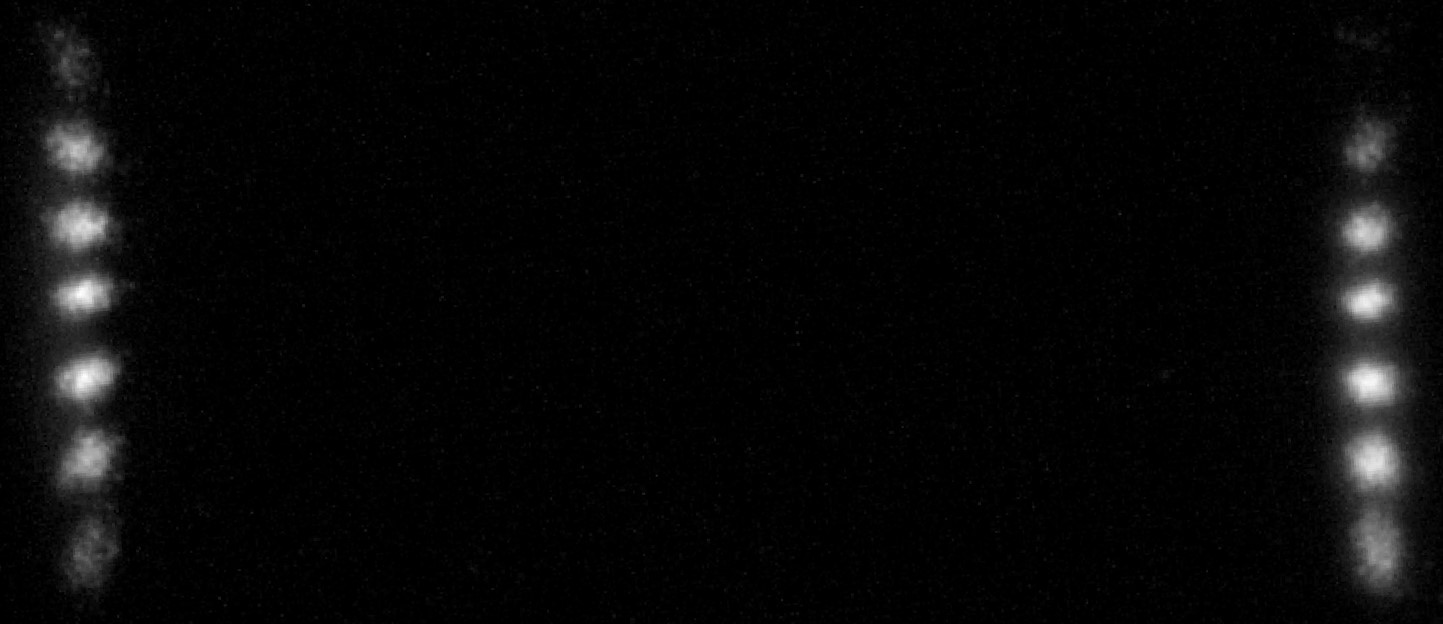
\includegraphics[width=0.5\linewidth]{part2/Figs/example_calibration.jpeg}
    \caption{An example of an image used to calibration the timing of the streaked pepperpots.}
    % Set 9 2017.06.11
    \label{figure:example_calibration}
\end{figure}

\subsection{Pepperpots}
There were a number of iterations on the precise configuration of the one- and two-dimensional pepperpots used in these experiments.
There are a number of considerations when designing pepperpot masks;
\begin{itemize}
    \item{\emph{Aperture size:} Smaller apertures provide a better resolution to the emittance measurement but reduce the signal as fewer particles pass through the hole.
    Aperture size affects the size of the beamlets on the detector, which impacts the overlap of beamlets on the detector, as the beamlets are a convolution of the aperture and the beam divergence. Smaller apertures also allow for a smaller aperture spacing as when the aperture diameter and aperture spacing are similar the pepperpot can become fragile.}
    \item{\emph{Aperture spacing:} Aperture spacing, also known as pitch, determines how well the full beam is sampled.
    Smaller pitch allows for better sampling of the full beam however pitch should be large enough that the beamlet overlap on the detector is manageable.
    If the pitch is too small then the pepperpot can also become fragile.}
    \item{\emph{Extent:} Ideally a the total extend of the pepperpot should be much larger than the largest beam for a particular apparatus.
    Unfortunately, due to the mounting arrangement of the Melbourne \gls{caeis}, the size of samples was limited to \unit[3]{mm} diameter and only a \unit[2]{mm} diameter portion of the sample was accessible to the beam. A view of the sample holder without the `lid' is shown in Figure~\ref{figure:sample_holder_pepperpots}.}
\end{itemize}

A number of restrictions aided the selection of parameters for the pepperpots used, the maximum pepperpot extent and need to focus the beam to the pepperpot size to maximise flux dictated the approximate size of the beamlets on the detector and thus the lowest feasibly pitch in order to minimise the overlap of beamlets on the detector.
The pepperpots were cut\footnote{The pepperpots were cut using a Oxford Laser Systems Alpha 532 laser micromachining system.} from \unit[25]{$\muup$ m} thick copper pinholes\footnote{Gilder Grids GA50-C3, \unit[50]{$\muup$ m} aperture.} with \unit[50]{$\muup$ m} diameter holes cut in the centre.
The central pinholes were used as the central aperture for the pepperpot arrays and since \unit[50]{$\muup$ m} apertures provide adequate flux the rest of the apertures were also cut to the same diameter to simplify analysis while providing acceptable measurement resolution.
A pitch of \unit[200]{$\muup$ m} was chosen to provide acceptable sampling of the beam while minimising the overlap of beamlets on the detector.
Given the \unit[2]{mm} diameter available this pitch allowed for one dimensional pepperpots with 7 apertures and two dimensional pepperpots with 7$\times$7 apertures.
The pepperpots used are shown in Figures~\ref{figure:pepperpot_mask} and \ref{figure:1d_pepperpot}.

\begin{figure}
    \center
    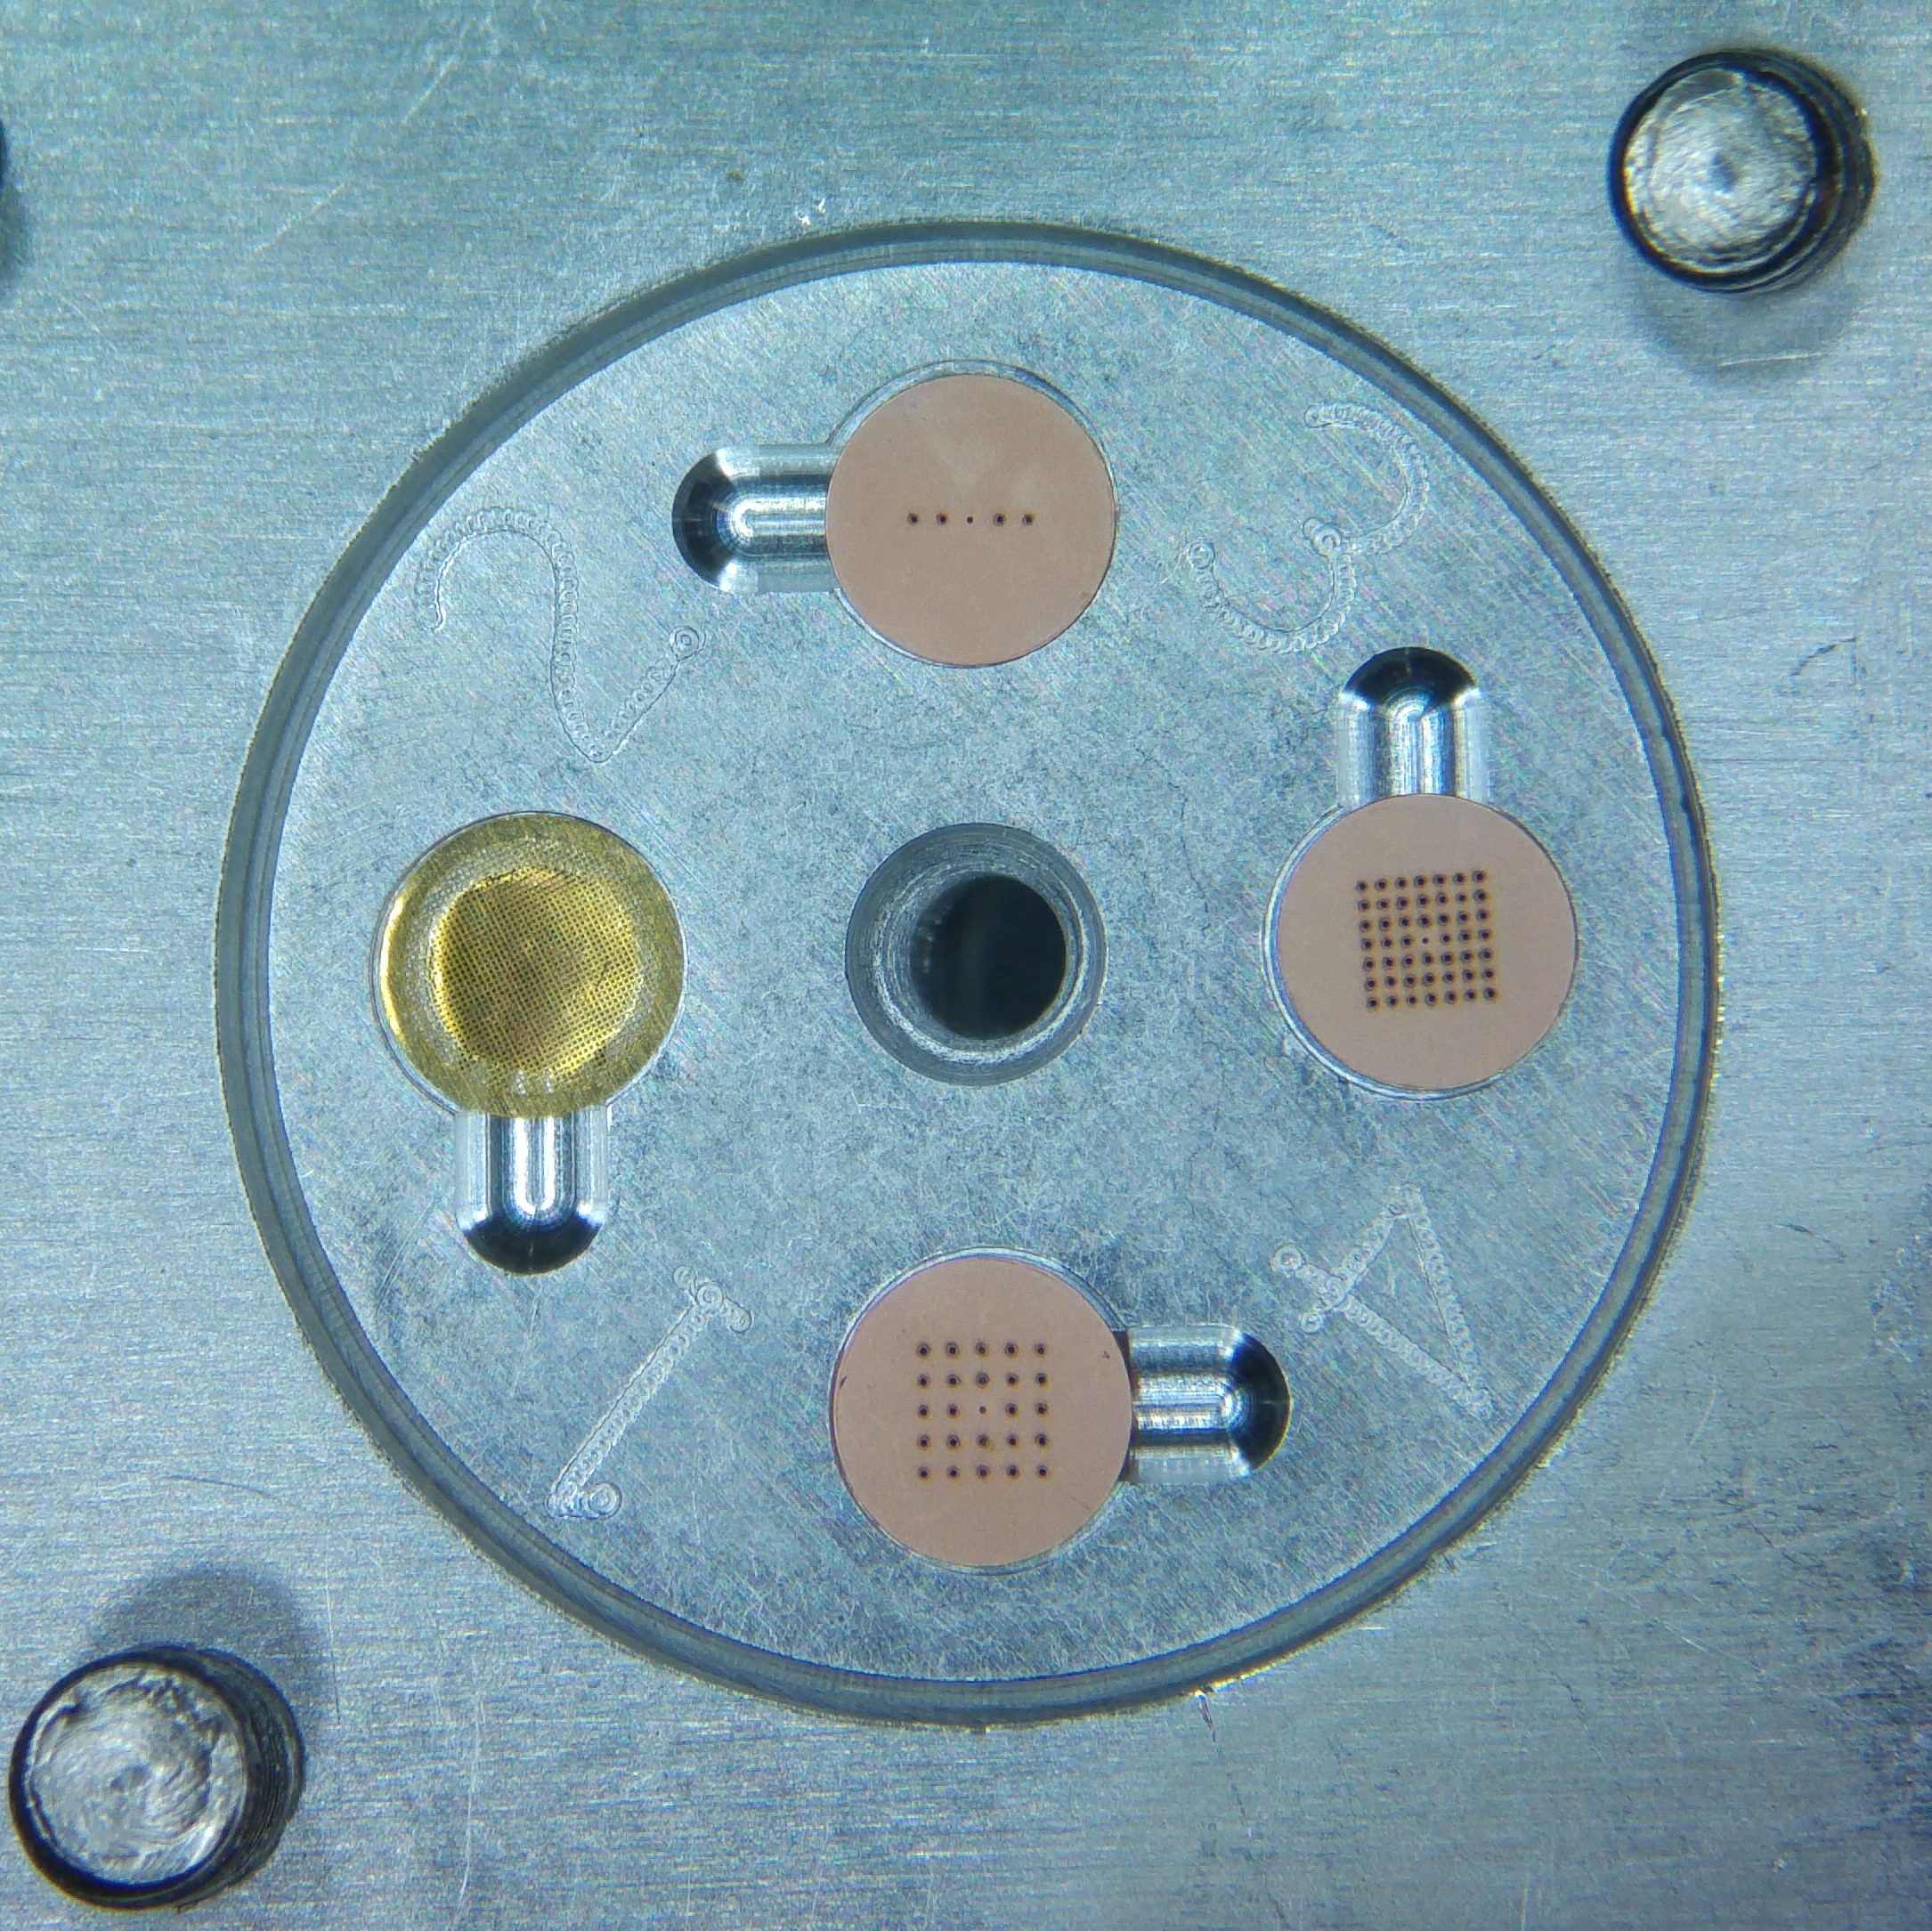
\includegraphics[width=0.49\linewidth]{part2/Figs/sample_holder.jpg}
    \caption{One of two sample holders that are used to load up to eight samples into the vacuum system. Clockwise from the top: five \unit[50]{$\muup$m} apertures with \unit[300]{$\muup$m} pitch, 7 by 7 pepperpot of \unit[50]{$\muup$m} apertures with \unit[200]{$\muup$m} pitch, 5 by 5 pepperpot of \unit[50]{$\muup$m} apertures with \unit[300]{$\muup$m} pitch, thin gold sample. Each sample is \unit[3]{mm} in diameter. A `lid' with appropriate apertures is placed over the samples to hold them in place.}
    \label{figure:sample_holder_pepperpots}
\end{figure}

\subsection{Laser Parameters}
Two of the lasers essential to the functioning are the `excitation' and `ionisation' lasers, see Section~\ref{section:two_stage_ionisation}, a CW red and pulsed blue laser respectively.
These lasers have a number of parameters that affect the emittance measurements.

\subsubsection{Excitation Laser}
The excitation laser was a \unit[780]{nm} laser, frequency locked to the Rb85 D2 F=3 to F=4 transition, which excites ground state atoms in the \gls{mot} to prepare the atoms for ionisation.
The spatial profile of this laser is highly controllable with a \gls{slm} allowing for arbitrary profiles to be mapped to the electron or ion bunch~\cite{mcculloch_arbitrarily_2011}.
The highest flux is possible by simply saturating the \gls{mot} however control over the electron beam profile and size is usually desirable.
One commonly used and simple distribution is a flat-top distribution as it can provide even electron intensity across the sample under examination however electron beams generated from electrons with high excess energy are unable to maintain the distribution, see Figure~\ref{figure:flat_top}.

\begin{figure}
    \center
    %% Creator: Matplotlib, PGF backend
%%
%% To include the figure in your LaTeX document, write
%%   \input{<filename>.pgf}
%%
%% Make sure the required packages are loaded in your preamble
%%   \usepackage{pgf}
%%
%% Figures using additional raster images can only be included by \input if
%% they are in the same directory as the main LaTeX file. For loading figures
%% from other directories you can use the `import` package
%%   \usepackage{import}
%% and then include the figures with
%%   \import{<path to file>}{<filename>.pgf}
%%
%% Matplotlib used the following preamble
%%
\begingroup%
\makeatletter%
\begin{pgfpicture}%
\pgfpathrectangle{\pgfpointorigin}{\pgfqpoint{5.424500in}{3.977967in}}%
\pgfusepath{use as bounding box, clip}%
\begin{pgfscope}%
\pgfsetbuttcap%
\pgfsetmiterjoin%
\definecolor{currentfill}{rgb}{1.000000,1.000000,1.000000}%
\pgfsetfillcolor{currentfill}%
\pgfsetlinewidth{0.000000pt}%
\definecolor{currentstroke}{rgb}{1.000000,1.000000,1.000000}%
\pgfsetstrokecolor{currentstroke}%
\pgfsetdash{}{0pt}%
\pgfpathmoveto{\pgfqpoint{0.000000in}{0.000000in}}%
\pgfpathlineto{\pgfqpoint{5.424500in}{0.000000in}}%
\pgfpathlineto{\pgfqpoint{5.424500in}{3.977967in}}%
\pgfpathlineto{\pgfqpoint{0.000000in}{3.977967in}}%
\pgfpathclose%
\pgfusepath{fill}%
\end{pgfscope}%
\begin{pgfscope}%
\pgfsetbuttcap%
\pgfsetmiterjoin%
\definecolor{currentfill}{rgb}{1.000000,1.000000,1.000000}%
\pgfsetfillcolor{currentfill}%
\pgfsetlinewidth{0.000000pt}%
\definecolor{currentstroke}{rgb}{0.000000,0.000000,0.000000}%
\pgfsetstrokecolor{currentstroke}%
\pgfsetstrokeopacity{0.000000}%
\pgfsetdash{}{0pt}%
\pgfpathmoveto{\pgfqpoint{0.396944in}{2.104261in}}%
\pgfpathlineto{\pgfqpoint{2.017796in}{2.104261in}}%
\pgfpathlineto{\pgfqpoint{2.017796in}{3.593522in}}%
\pgfpathlineto{\pgfqpoint{0.396944in}{3.593522in}}%
\pgfpathclose%
\pgfusepath{fill}%
\end{pgfscope}%
\begin{pgfscope}%
\pgfpathrectangle{\pgfqpoint{0.396944in}{2.104261in}}{\pgfqpoint{1.620852in}{1.489261in}} %
\pgfusepath{clip}%
\pgftext[at=\pgfqpoint{0.396944in}{2.104261in},left,bottom]{\pgfimage[interpolate=true,width=1.630000in,height=1.500000in]{flattops_emittance-img0.png}}%
\end{pgfscope}%
\begin{pgfscope}%
\pgfpathrectangle{\pgfqpoint{0.396944in}{2.104261in}}{\pgfqpoint{1.620852in}{1.489261in}} %
\pgfusepath{clip}%
\pgfsetbuttcap%
\pgfsetroundjoin%
\pgfsetlinewidth{1.003750pt}%
\definecolor{currentstroke}{rgb}{1.000000,1.000000,1.000000}%
\pgfsetstrokecolor{currentstroke}%
\pgfsetdash{{6.000000pt}{6.000000pt}}{0.000000pt}%
\pgfpathmoveto{\pgfqpoint{0.396944in}{2.846410in}}%
\pgfpathlineto{\pgfqpoint{2.017796in}{2.846410in}}%
\pgfusepath{stroke}%
\end{pgfscope}%
\begin{pgfscope}%
\pgfsetrectcap%
\pgfsetmiterjoin%
\pgfsetlinewidth{1.003750pt}%
\definecolor{currentstroke}{rgb}{0.000000,0.000000,0.000000}%
\pgfsetstrokecolor{currentstroke}%
\pgfsetdash{}{0pt}%
\pgfpathmoveto{\pgfqpoint{0.396944in}{2.104261in}}%
\pgfpathlineto{\pgfqpoint{0.396944in}{3.593522in}}%
\pgfusepath{stroke}%
\end{pgfscope}%
\begin{pgfscope}%
\pgfsetrectcap%
\pgfsetmiterjoin%
\pgfsetlinewidth{1.003750pt}%
\definecolor{currentstroke}{rgb}{0.000000,0.000000,0.000000}%
\pgfsetstrokecolor{currentstroke}%
\pgfsetdash{}{0pt}%
\pgfpathmoveto{\pgfqpoint{0.396944in}{2.104261in}}%
\pgfpathlineto{\pgfqpoint{2.017796in}{2.104261in}}%
\pgfusepath{stroke}%
\end{pgfscope}%
\begin{pgfscope}%
\pgfsetrectcap%
\pgfsetmiterjoin%
\pgfsetlinewidth{1.003750pt}%
\definecolor{currentstroke}{rgb}{0.000000,0.000000,0.000000}%
\pgfsetstrokecolor{currentstroke}%
\pgfsetdash{}{0pt}%
\pgfpathmoveto{\pgfqpoint{0.396944in}{3.593522in}}%
\pgfpathlineto{\pgfqpoint{2.017796in}{3.593522in}}%
\pgfusepath{stroke}%
\end{pgfscope}%
\begin{pgfscope}%
\pgfsetrectcap%
\pgfsetmiterjoin%
\pgfsetlinewidth{1.003750pt}%
\definecolor{currentstroke}{rgb}{0.000000,0.000000,0.000000}%
\pgfsetstrokecolor{currentstroke}%
\pgfsetdash{}{0pt}%
\pgfpathmoveto{\pgfqpoint{2.017796in}{2.104261in}}%
\pgfpathlineto{\pgfqpoint{2.017796in}{3.593522in}}%
\pgfusepath{stroke}%
\end{pgfscope}%
\begin{pgfscope}%
\pgftext[x=1.207370in,y=3.662967in,,base]{\rmfamily\fontsize{13.200000}{15.840000}\selectfont -42.0\(\displaystyle \,\)meV}%
\end{pgfscope}%
\begin{pgfscope}%
\pgfsetbuttcap%
\pgfsetmiterjoin%
\definecolor{currentfill}{rgb}{1.000000,1.000000,1.000000}%
\pgfsetfillcolor{currentfill}%
\pgfsetlinewidth{0.000000pt}%
\definecolor{currentstroke}{rgb}{0.000000,0.000000,0.000000}%
\pgfsetstrokecolor{currentstroke}%
\pgfsetstrokeopacity{0.000000}%
\pgfsetdash{}{0pt}%
\pgfpathmoveto{\pgfqpoint{0.396944in}{0.615000in}}%
\pgfpathlineto{\pgfqpoint{2.017796in}{0.615000in}}%
\pgfpathlineto{\pgfqpoint{2.017796in}{2.104261in}}%
\pgfpathlineto{\pgfqpoint{0.396944in}{2.104261in}}%
\pgfpathclose%
\pgfusepath{fill}%
\end{pgfscope}%
\begin{pgfscope}%
\pgfpathrectangle{\pgfqpoint{0.396944in}{0.615000in}}{\pgfqpoint{1.620852in}{1.489261in}} %
\pgfusepath{clip}%
\pgfsetbuttcap%
\pgfsetroundjoin%
\pgfsetlinewidth{1.003750pt}%
\definecolor{currentstroke}{rgb}{1.000000,0.000000,0.000000}%
\pgfsetstrokecolor{currentstroke}%
\pgfsetdash{{1.000000pt}{3.000000pt}}{0.000000pt}%
\pgfpathmoveto{\pgfqpoint{0.396944in}{0.624506in}}%
\pgfpathlineto{\pgfqpoint{0.402347in}{0.617183in}}%
\pgfpathlineto{\pgfqpoint{0.407750in}{0.615000in}}%
\pgfpathlineto{\pgfqpoint{0.413153in}{0.615830in}}%
\pgfpathlineto{\pgfqpoint{0.418556in}{0.618413in}}%
\pgfpathlineto{\pgfqpoint{0.434764in}{0.633164in}}%
\pgfpathlineto{\pgfqpoint{0.445570in}{0.631717in}}%
\pgfpathlineto{\pgfqpoint{0.450973in}{0.629860in}}%
\pgfpathlineto{\pgfqpoint{0.456376in}{0.633103in}}%
\pgfpathlineto{\pgfqpoint{0.461779in}{0.641380in}}%
\pgfpathlineto{\pgfqpoint{0.472584in}{0.653406in}}%
\pgfpathlineto{\pgfqpoint{0.477987in}{0.663637in}}%
\pgfpathlineto{\pgfqpoint{0.488793in}{0.674176in}}%
\pgfpathlineto{\pgfqpoint{0.494196in}{0.674855in}}%
\pgfpathlineto{\pgfqpoint{0.499598in}{0.680154in}}%
\pgfpathlineto{\pgfqpoint{0.505001in}{0.682156in}}%
\pgfpathlineto{\pgfqpoint{0.510404in}{0.692276in}}%
\pgfpathlineto{\pgfqpoint{0.515807in}{0.698970in}}%
\pgfpathlineto{\pgfqpoint{0.521210in}{0.701174in}}%
\pgfpathlineto{\pgfqpoint{0.532015in}{0.725330in}}%
\pgfpathlineto{\pgfqpoint{0.542821in}{0.753712in}}%
\pgfpathlineto{\pgfqpoint{0.548224in}{0.764961in}}%
\pgfpathlineto{\pgfqpoint{0.559030in}{0.773106in}}%
\pgfpathlineto{\pgfqpoint{0.564432in}{0.782553in}}%
\pgfpathlineto{\pgfqpoint{0.569835in}{0.795326in}}%
\pgfpathlineto{\pgfqpoint{0.580641in}{0.828780in}}%
\pgfpathlineto{\pgfqpoint{0.591447in}{0.846073in}}%
\pgfpathlineto{\pgfqpoint{0.596850in}{0.848364in}}%
\pgfpathlineto{\pgfqpoint{0.613058in}{0.908456in}}%
\pgfpathlineto{\pgfqpoint{0.623864in}{0.937368in}}%
\pgfpathlineto{\pgfqpoint{0.629267in}{0.949366in}}%
\pgfpathlineto{\pgfqpoint{0.640072in}{0.984131in}}%
\pgfpathlineto{\pgfqpoint{0.645475in}{0.996817in}}%
\pgfpathlineto{\pgfqpoint{0.650878in}{1.015002in}}%
\pgfpathlineto{\pgfqpoint{0.656281in}{1.023664in}}%
\pgfpathlineto{\pgfqpoint{0.661684in}{1.037305in}}%
\pgfpathlineto{\pgfqpoint{0.667086in}{1.043856in}}%
\pgfpathlineto{\pgfqpoint{0.683295in}{1.095942in}}%
\pgfpathlineto{\pgfqpoint{0.688698in}{1.110675in}}%
\pgfpathlineto{\pgfqpoint{0.694101in}{1.133854in}}%
\pgfpathlineto{\pgfqpoint{0.699503in}{1.144489in}}%
\pgfpathlineto{\pgfqpoint{0.704906in}{1.161049in}}%
\pgfpathlineto{\pgfqpoint{0.710309in}{1.186676in}}%
\pgfpathlineto{\pgfqpoint{0.715712in}{1.198221in}}%
\pgfpathlineto{\pgfqpoint{0.726518in}{1.217748in}}%
\pgfpathlineto{\pgfqpoint{0.731920in}{1.247198in}}%
\pgfpathlineto{\pgfqpoint{0.742726in}{1.291361in}}%
\pgfpathlineto{\pgfqpoint{0.753532in}{1.329699in}}%
\pgfpathlineto{\pgfqpoint{0.758935in}{1.330222in}}%
\pgfpathlineto{\pgfqpoint{0.764338in}{1.337509in}}%
\pgfpathlineto{\pgfqpoint{0.769740in}{1.352766in}}%
\pgfpathlineto{\pgfqpoint{0.775143in}{1.377587in}}%
\pgfpathlineto{\pgfqpoint{0.780546in}{1.395487in}}%
\pgfpathlineto{\pgfqpoint{0.785949in}{1.425367in}}%
\pgfpathlineto{\pgfqpoint{0.791352in}{1.447276in}}%
\pgfpathlineto{\pgfqpoint{0.796755in}{1.454341in}}%
\pgfpathlineto{\pgfqpoint{0.802157in}{1.456747in}}%
\pgfpathlineto{\pgfqpoint{0.807560in}{1.466169in}}%
\pgfpathlineto{\pgfqpoint{0.812963in}{1.478067in}}%
\pgfpathlineto{\pgfqpoint{0.818366in}{1.500692in}}%
\pgfpathlineto{\pgfqpoint{0.823769in}{1.506510in}}%
\pgfpathlineto{\pgfqpoint{0.834574in}{1.500069in}}%
\pgfpathlineto{\pgfqpoint{0.845380in}{1.517184in}}%
\pgfpathlineto{\pgfqpoint{0.861589in}{1.609881in}}%
\pgfpathlineto{\pgfqpoint{0.872394in}{1.625364in}}%
\pgfpathlineto{\pgfqpoint{0.877797in}{1.641911in}}%
\pgfpathlineto{\pgfqpoint{0.883200in}{1.676034in}}%
\pgfpathlineto{\pgfqpoint{0.888603in}{1.696906in}}%
\pgfpathlineto{\pgfqpoint{0.904811in}{1.705828in}}%
\pgfpathlineto{\pgfqpoint{0.910214in}{1.698244in}}%
\pgfpathlineto{\pgfqpoint{0.915617in}{1.704252in}}%
\pgfpathlineto{\pgfqpoint{0.921020in}{1.717012in}}%
\pgfpathlineto{\pgfqpoint{0.926423in}{1.746840in}}%
\pgfpathlineto{\pgfqpoint{0.931826in}{1.743679in}}%
\pgfpathlineto{\pgfqpoint{0.937228in}{1.742522in}}%
\pgfpathlineto{\pgfqpoint{0.942631in}{1.723305in}}%
\pgfpathlineto{\pgfqpoint{0.948034in}{1.711510in}}%
\pgfpathlineto{\pgfqpoint{0.953437in}{1.731151in}}%
\pgfpathlineto{\pgfqpoint{0.964243in}{1.758237in}}%
\pgfpathlineto{\pgfqpoint{0.969645in}{1.770696in}}%
\pgfpathlineto{\pgfqpoint{0.975048in}{1.763072in}}%
\pgfpathlineto{\pgfqpoint{0.980451in}{1.743022in}}%
\pgfpathlineto{\pgfqpoint{0.985854in}{1.741979in}}%
\pgfpathlineto{\pgfqpoint{0.991257in}{1.768678in}}%
\pgfpathlineto{\pgfqpoint{1.002062in}{1.804722in}}%
\pgfpathlineto{\pgfqpoint{1.012868in}{1.800859in}}%
\pgfpathlineto{\pgfqpoint{1.018271in}{1.804120in}}%
\pgfpathlineto{\pgfqpoint{1.023674in}{1.809490in}}%
\pgfpathlineto{\pgfqpoint{1.029077in}{1.830170in}}%
\pgfpathlineto{\pgfqpoint{1.034480in}{1.855304in}}%
\pgfpathlineto{\pgfqpoint{1.039882in}{1.850514in}}%
\pgfpathlineto{\pgfqpoint{1.045285in}{1.849056in}}%
\pgfpathlineto{\pgfqpoint{1.050688in}{1.845176in}}%
\pgfpathlineto{\pgfqpoint{1.056091in}{1.847910in}}%
\pgfpathlineto{\pgfqpoint{1.066897in}{1.918792in}}%
\pgfpathlineto{\pgfqpoint{1.072299in}{1.936413in}}%
\pgfpathlineto{\pgfqpoint{1.077702in}{1.942640in}}%
\pgfpathlineto{\pgfqpoint{1.083105in}{1.919165in}}%
\pgfpathlineto{\pgfqpoint{1.088508in}{1.929888in}}%
\pgfpathlineto{\pgfqpoint{1.093911in}{1.949997in}}%
\pgfpathlineto{\pgfqpoint{1.099314in}{1.984919in}}%
\pgfpathlineto{\pgfqpoint{1.104716in}{1.997039in}}%
\pgfpathlineto{\pgfqpoint{1.110119in}{1.985391in}}%
\pgfpathlineto{\pgfqpoint{1.115522in}{1.979564in}}%
\pgfpathlineto{\pgfqpoint{1.120925in}{1.993797in}}%
\pgfpathlineto{\pgfqpoint{1.131731in}{2.014487in}}%
\pgfpathlineto{\pgfqpoint{1.137133in}{2.028705in}}%
\pgfpathlineto{\pgfqpoint{1.147939in}{2.005485in}}%
\pgfpathlineto{\pgfqpoint{1.153342in}{1.978272in}}%
\pgfpathlineto{\pgfqpoint{1.158745in}{1.991513in}}%
\pgfpathlineto{\pgfqpoint{1.164148in}{1.999734in}}%
\pgfpathlineto{\pgfqpoint{1.169550in}{2.021193in}}%
\pgfpathlineto{\pgfqpoint{1.174953in}{2.033344in}}%
\pgfpathlineto{\pgfqpoint{1.180356in}{2.021453in}}%
\pgfpathlineto{\pgfqpoint{1.191162in}{1.975564in}}%
\pgfpathlineto{\pgfqpoint{1.196565in}{1.979900in}}%
\pgfpathlineto{\pgfqpoint{1.201968in}{1.996861in}}%
\pgfpathlineto{\pgfqpoint{1.207370in}{2.017661in}}%
\pgfpathlineto{\pgfqpoint{1.218176in}{2.001975in}}%
\pgfpathlineto{\pgfqpoint{1.228982in}{1.963851in}}%
\pgfpathlineto{\pgfqpoint{1.234385in}{1.983969in}}%
\pgfpathlineto{\pgfqpoint{1.239787in}{2.015341in}}%
\pgfpathlineto{\pgfqpoint{1.245190in}{2.015105in}}%
\pgfpathlineto{\pgfqpoint{1.250593in}{1.986095in}}%
\pgfpathlineto{\pgfqpoint{1.261399in}{1.953630in}}%
\pgfpathlineto{\pgfqpoint{1.266802in}{1.949386in}}%
\pgfpathlineto{\pgfqpoint{1.272204in}{1.966186in}}%
\pgfpathlineto{\pgfqpoint{1.277607in}{1.958593in}}%
\pgfpathlineto{\pgfqpoint{1.283010in}{1.955774in}}%
\pgfpathlineto{\pgfqpoint{1.293816in}{1.916153in}}%
\pgfpathlineto{\pgfqpoint{1.299219in}{1.912828in}}%
\pgfpathlineto{\pgfqpoint{1.304621in}{1.916281in}}%
\pgfpathlineto{\pgfqpoint{1.310024in}{1.929046in}}%
\pgfpathlineto{\pgfqpoint{1.320830in}{1.911792in}}%
\pgfpathlineto{\pgfqpoint{1.331636in}{1.881268in}}%
\pgfpathlineto{\pgfqpoint{1.337039in}{1.890023in}}%
\pgfpathlineto{\pgfqpoint{1.342441in}{1.905559in}}%
\pgfpathlineto{\pgfqpoint{1.347844in}{1.914307in}}%
\pgfpathlineto{\pgfqpoint{1.358650in}{1.901259in}}%
\pgfpathlineto{\pgfqpoint{1.364053in}{1.879160in}}%
\pgfpathlineto{\pgfqpoint{1.369456in}{1.868038in}}%
\pgfpathlineto{\pgfqpoint{1.374858in}{1.869194in}}%
\pgfpathlineto{\pgfqpoint{1.380261in}{1.891658in}}%
\pgfpathlineto{\pgfqpoint{1.385664in}{1.898922in}}%
\pgfpathlineto{\pgfqpoint{1.391067in}{1.884713in}}%
\pgfpathlineto{\pgfqpoint{1.396470in}{1.850157in}}%
\pgfpathlineto{\pgfqpoint{1.401873in}{1.825040in}}%
\pgfpathlineto{\pgfqpoint{1.407275in}{1.821226in}}%
\pgfpathlineto{\pgfqpoint{1.412678in}{1.826164in}}%
\pgfpathlineto{\pgfqpoint{1.418081in}{1.814499in}}%
\pgfpathlineto{\pgfqpoint{1.423484in}{1.806746in}}%
\pgfpathlineto{\pgfqpoint{1.428887in}{1.786458in}}%
\pgfpathlineto{\pgfqpoint{1.439692in}{1.717497in}}%
\pgfpathlineto{\pgfqpoint{1.445095in}{1.736045in}}%
\pgfpathlineto{\pgfqpoint{1.455901in}{1.783806in}}%
\pgfpathlineto{\pgfqpoint{1.461304in}{1.778362in}}%
\pgfpathlineto{\pgfqpoint{1.466707in}{1.759812in}}%
\pgfpathlineto{\pgfqpoint{1.472110in}{1.725997in}}%
\pgfpathlineto{\pgfqpoint{1.477512in}{1.745386in}}%
\pgfpathlineto{\pgfqpoint{1.482915in}{1.737790in}}%
\pgfpathlineto{\pgfqpoint{1.488318in}{1.726730in}}%
\pgfpathlineto{\pgfqpoint{1.499124in}{1.692137in}}%
\pgfpathlineto{\pgfqpoint{1.504527in}{1.657320in}}%
\pgfpathlineto{\pgfqpoint{1.515332in}{1.611988in}}%
\pgfpathlineto{\pgfqpoint{1.520735in}{1.620910in}}%
\pgfpathlineto{\pgfqpoint{1.526138in}{1.609485in}}%
\pgfpathlineto{\pgfqpoint{1.531541in}{1.592182in}}%
\pgfpathlineto{\pgfqpoint{1.536944in}{1.565616in}}%
\pgfpathlineto{\pgfqpoint{1.542346in}{1.530017in}}%
\pgfpathlineto{\pgfqpoint{1.547749in}{1.513145in}}%
\pgfpathlineto{\pgfqpoint{1.553152in}{1.506941in}}%
\pgfpathlineto{\pgfqpoint{1.563958in}{1.488595in}}%
\pgfpathlineto{\pgfqpoint{1.569361in}{1.490645in}}%
\pgfpathlineto{\pgfqpoint{1.580166in}{1.446096in}}%
\pgfpathlineto{\pgfqpoint{1.585569in}{1.435569in}}%
\pgfpathlineto{\pgfqpoint{1.590972in}{1.434589in}}%
\pgfpathlineto{\pgfqpoint{1.596375in}{1.426068in}}%
\pgfpathlineto{\pgfqpoint{1.601778in}{1.413680in}}%
\pgfpathlineto{\pgfqpoint{1.607180in}{1.389409in}}%
\pgfpathlineto{\pgfqpoint{1.617986in}{1.325803in}}%
\pgfpathlineto{\pgfqpoint{1.623389in}{1.309119in}}%
\pgfpathlineto{\pgfqpoint{1.645000in}{1.228860in}}%
\pgfpathlineto{\pgfqpoint{1.650403in}{1.198382in}}%
\pgfpathlineto{\pgfqpoint{1.655806in}{1.174633in}}%
\pgfpathlineto{\pgfqpoint{1.661209in}{1.160604in}}%
\pgfpathlineto{\pgfqpoint{1.672015in}{1.120440in}}%
\pgfpathlineto{\pgfqpoint{1.677417in}{1.107922in}}%
\pgfpathlineto{\pgfqpoint{1.682820in}{1.089267in}}%
\pgfpathlineto{\pgfqpoint{1.688223in}{1.094514in}}%
\pgfpathlineto{\pgfqpoint{1.693626in}{1.083771in}}%
\pgfpathlineto{\pgfqpoint{1.699029in}{1.057427in}}%
\pgfpathlineto{\pgfqpoint{1.709834in}{0.999439in}}%
\pgfpathlineto{\pgfqpoint{1.715237in}{0.990971in}}%
\pgfpathlineto{\pgfqpoint{1.720640in}{0.976461in}}%
\pgfpathlineto{\pgfqpoint{1.731446in}{0.959648in}}%
\pgfpathlineto{\pgfqpoint{1.747654in}{0.905056in}}%
\pgfpathlineto{\pgfqpoint{1.758460in}{0.860632in}}%
\pgfpathlineto{\pgfqpoint{1.763863in}{0.859552in}}%
\pgfpathlineto{\pgfqpoint{1.769266in}{0.843635in}}%
\pgfpathlineto{\pgfqpoint{1.785474in}{0.806525in}}%
\pgfpathlineto{\pgfqpoint{1.790877in}{0.793159in}}%
\pgfpathlineto{\pgfqpoint{1.801683in}{0.779348in}}%
\pgfpathlineto{\pgfqpoint{1.817891in}{0.740778in}}%
\pgfpathlineto{\pgfqpoint{1.823294in}{0.736172in}}%
\pgfpathlineto{\pgfqpoint{1.828697in}{0.735359in}}%
\pgfpathlineto{\pgfqpoint{1.839503in}{0.738763in}}%
\pgfpathlineto{\pgfqpoint{1.844905in}{0.729006in}}%
\pgfpathlineto{\pgfqpoint{1.850308in}{0.725054in}}%
\pgfpathlineto{\pgfqpoint{1.861114in}{0.727545in}}%
\pgfpathlineto{\pgfqpoint{1.866517in}{0.726100in}}%
\pgfpathlineto{\pgfqpoint{1.871920in}{0.723010in}}%
\pgfpathlineto{\pgfqpoint{1.877322in}{0.713266in}}%
\pgfpathlineto{\pgfqpoint{1.882725in}{0.706297in}}%
\pgfpathlineto{\pgfqpoint{1.888128in}{0.694800in}}%
\pgfpathlineto{\pgfqpoint{1.893531in}{0.686121in}}%
\pgfpathlineto{\pgfqpoint{1.898934in}{0.683309in}}%
\pgfpathlineto{\pgfqpoint{1.904337in}{0.683408in}}%
\pgfpathlineto{\pgfqpoint{1.915142in}{0.673374in}}%
\pgfpathlineto{\pgfqpoint{1.920545in}{0.670289in}}%
\pgfpathlineto{\pgfqpoint{1.925948in}{0.664697in}}%
\pgfpathlineto{\pgfqpoint{1.931351in}{0.664232in}}%
\pgfpathlineto{\pgfqpoint{1.936754in}{0.670154in}}%
\pgfpathlineto{\pgfqpoint{1.942157in}{0.678123in}}%
\pgfpathlineto{\pgfqpoint{1.947559in}{0.681880in}}%
\pgfpathlineto{\pgfqpoint{1.952962in}{0.679534in}}%
\pgfpathlineto{\pgfqpoint{1.958365in}{0.674227in}}%
\pgfpathlineto{\pgfqpoint{1.963768in}{0.666296in}}%
\pgfpathlineto{\pgfqpoint{1.969171in}{0.673768in}}%
\pgfpathlineto{\pgfqpoint{1.974574in}{0.684694in}}%
\pgfpathlineto{\pgfqpoint{1.979976in}{0.685555in}}%
\pgfpathlineto{\pgfqpoint{1.985379in}{0.681985in}}%
\pgfpathlineto{\pgfqpoint{1.990782in}{0.672626in}}%
\pgfpathlineto{\pgfqpoint{1.996185in}{0.666338in}}%
\pgfpathlineto{\pgfqpoint{2.012393in}{0.665880in}}%
\pgfpathlineto{\pgfqpoint{2.012393in}{0.665880in}}%
\pgfusepath{stroke}%
\end{pgfscope}%
\begin{pgfscope}%
\pgfpathrectangle{\pgfqpoint{0.396944in}{0.615000in}}{\pgfqpoint{1.620852in}{1.489261in}} %
\pgfusepath{clip}%
\pgfsetrectcap%
\pgfsetroundjoin%
\pgfsetlinewidth{1.003750pt}%
\definecolor{currentstroke}{rgb}{0.000000,0.000000,1.000000}%
\pgfsetstrokecolor{currentstroke}%
\pgfsetdash{}{0pt}%
\pgfpathmoveto{\pgfqpoint{0.396944in}{0.615000in}}%
\pgfpathlineto{\pgfqpoint{0.402347in}{0.618912in}}%
\pgfpathlineto{\pgfqpoint{0.407750in}{0.619150in}}%
\pgfpathlineto{\pgfqpoint{0.413153in}{0.621395in}}%
\pgfpathlineto{\pgfqpoint{0.423959in}{0.622383in}}%
\pgfpathlineto{\pgfqpoint{0.434764in}{0.619500in}}%
\pgfpathlineto{\pgfqpoint{0.450973in}{0.624916in}}%
\pgfpathlineto{\pgfqpoint{0.456376in}{0.621067in}}%
\pgfpathlineto{\pgfqpoint{0.461779in}{0.621715in}}%
\pgfpathlineto{\pgfqpoint{0.467181in}{0.624334in}}%
\pgfpathlineto{\pgfqpoint{0.472584in}{0.622872in}}%
\pgfpathlineto{\pgfqpoint{0.483390in}{0.623885in}}%
\pgfpathlineto{\pgfqpoint{0.488793in}{0.628712in}}%
\pgfpathlineto{\pgfqpoint{0.494196in}{0.630422in}}%
\pgfpathlineto{\pgfqpoint{0.510404in}{0.631175in}}%
\pgfpathlineto{\pgfqpoint{0.515807in}{0.639049in}}%
\pgfpathlineto{\pgfqpoint{0.521210in}{0.638590in}}%
\pgfpathlineto{\pgfqpoint{0.537418in}{0.629095in}}%
\pgfpathlineto{\pgfqpoint{0.542821in}{0.629626in}}%
\pgfpathlineto{\pgfqpoint{0.548224in}{0.632354in}}%
\pgfpathlineto{\pgfqpoint{0.553627in}{0.631579in}}%
\pgfpathlineto{\pgfqpoint{0.564432in}{0.643352in}}%
\pgfpathlineto{\pgfqpoint{0.575238in}{0.645350in}}%
\pgfpathlineto{\pgfqpoint{0.596850in}{0.658271in}}%
\pgfpathlineto{\pgfqpoint{0.602252in}{0.659259in}}%
\pgfpathlineto{\pgfqpoint{0.613058in}{0.652909in}}%
\pgfpathlineto{\pgfqpoint{0.623864in}{0.647374in}}%
\pgfpathlineto{\pgfqpoint{0.634669in}{0.653351in}}%
\pgfpathlineto{\pgfqpoint{0.645475in}{0.656883in}}%
\pgfpathlineto{\pgfqpoint{0.661684in}{0.669351in}}%
\pgfpathlineto{\pgfqpoint{0.672489in}{0.664428in}}%
\pgfpathlineto{\pgfqpoint{0.688698in}{0.677051in}}%
\pgfpathlineto{\pgfqpoint{0.704906in}{0.692320in}}%
\pgfpathlineto{\pgfqpoint{0.710309in}{0.705349in}}%
\pgfpathlineto{\pgfqpoint{0.715712in}{0.711165in}}%
\pgfpathlineto{\pgfqpoint{0.726518in}{0.726586in}}%
\pgfpathlineto{\pgfqpoint{0.737323in}{0.736936in}}%
\pgfpathlineto{\pgfqpoint{0.742726in}{0.743867in}}%
\pgfpathlineto{\pgfqpoint{0.753532in}{0.764385in}}%
\pgfpathlineto{\pgfqpoint{0.758935in}{0.777190in}}%
\pgfpathlineto{\pgfqpoint{0.769740in}{0.790451in}}%
\pgfpathlineto{\pgfqpoint{0.775143in}{0.800330in}}%
\pgfpathlineto{\pgfqpoint{0.780546in}{0.817574in}}%
\pgfpathlineto{\pgfqpoint{0.785949in}{0.824454in}}%
\pgfpathlineto{\pgfqpoint{0.796755in}{0.881494in}}%
\pgfpathlineto{\pgfqpoint{0.802157in}{0.908844in}}%
\pgfpathlineto{\pgfqpoint{0.807560in}{0.927323in}}%
\pgfpathlineto{\pgfqpoint{0.812963in}{0.941603in}}%
\pgfpathlineto{\pgfqpoint{0.829172in}{1.035107in}}%
\pgfpathlineto{\pgfqpoint{0.839977in}{1.150685in}}%
\pgfpathlineto{\pgfqpoint{0.856186in}{1.276340in}}%
\pgfpathlineto{\pgfqpoint{0.866991in}{1.385634in}}%
\pgfpathlineto{\pgfqpoint{0.899409in}{1.664456in}}%
\pgfpathlineto{\pgfqpoint{0.910214in}{1.714582in}}%
\pgfpathlineto{\pgfqpoint{0.915617in}{1.741586in}}%
\pgfpathlineto{\pgfqpoint{0.921020in}{1.751345in}}%
\pgfpathlineto{\pgfqpoint{0.926423in}{1.765812in}}%
\pgfpathlineto{\pgfqpoint{0.937228in}{1.849557in}}%
\pgfpathlineto{\pgfqpoint{0.942631in}{1.881232in}}%
\pgfpathlineto{\pgfqpoint{0.948034in}{1.874213in}}%
\pgfpathlineto{\pgfqpoint{0.953437in}{1.864884in}}%
\pgfpathlineto{\pgfqpoint{0.958840in}{1.868372in}}%
\pgfpathlineto{\pgfqpoint{0.964243in}{1.909196in}}%
\pgfpathlineto{\pgfqpoint{0.969645in}{1.927995in}}%
\pgfpathlineto{\pgfqpoint{0.975048in}{1.956620in}}%
\pgfpathlineto{\pgfqpoint{0.980451in}{1.961832in}}%
\pgfpathlineto{\pgfqpoint{0.985854in}{1.946864in}}%
\pgfpathlineto{\pgfqpoint{0.991257in}{1.942413in}}%
\pgfpathlineto{\pgfqpoint{0.996660in}{1.941014in}}%
\pgfpathlineto{\pgfqpoint{1.007465in}{1.992551in}}%
\pgfpathlineto{\pgfqpoint{1.012868in}{2.001597in}}%
\pgfpathlineto{\pgfqpoint{1.018271in}{1.990121in}}%
\pgfpathlineto{\pgfqpoint{1.023674in}{1.983319in}}%
\pgfpathlineto{\pgfqpoint{1.029077in}{1.985403in}}%
\pgfpathlineto{\pgfqpoint{1.034480in}{1.989844in}}%
\pgfpathlineto{\pgfqpoint{1.039882in}{2.008424in}}%
\pgfpathlineto{\pgfqpoint{1.045285in}{2.014164in}}%
\pgfpathlineto{\pgfqpoint{1.050688in}{1.990540in}}%
\pgfpathlineto{\pgfqpoint{1.056091in}{1.986105in}}%
\pgfpathlineto{\pgfqpoint{1.061494in}{1.992867in}}%
\pgfpathlineto{\pgfqpoint{1.066897in}{2.002957in}}%
\pgfpathlineto{\pgfqpoint{1.072299in}{2.003725in}}%
\pgfpathlineto{\pgfqpoint{1.077702in}{2.006272in}}%
\pgfpathlineto{\pgfqpoint{1.083105in}{1.996150in}}%
\pgfpathlineto{\pgfqpoint{1.093911in}{1.933907in}}%
\pgfpathlineto{\pgfqpoint{1.099314in}{1.918172in}}%
\pgfpathlineto{\pgfqpoint{1.104716in}{1.922672in}}%
\pgfpathlineto{\pgfqpoint{1.110119in}{1.950718in}}%
\pgfpathlineto{\pgfqpoint{1.115522in}{1.960164in}}%
\pgfpathlineto{\pgfqpoint{1.120925in}{1.955657in}}%
\pgfpathlineto{\pgfqpoint{1.126328in}{1.946150in}}%
\pgfpathlineto{\pgfqpoint{1.131731in}{1.933755in}}%
\pgfpathlineto{\pgfqpoint{1.137133in}{1.935600in}}%
\pgfpathlineto{\pgfqpoint{1.153342in}{1.931738in}}%
\pgfpathlineto{\pgfqpoint{1.158745in}{1.913619in}}%
\pgfpathlineto{\pgfqpoint{1.164148in}{1.888089in}}%
\pgfpathlineto{\pgfqpoint{1.169550in}{1.868714in}}%
\pgfpathlineto{\pgfqpoint{1.174953in}{1.872597in}}%
\pgfpathlineto{\pgfqpoint{1.180356in}{1.904971in}}%
\pgfpathlineto{\pgfqpoint{1.185759in}{1.906235in}}%
\pgfpathlineto{\pgfqpoint{1.196565in}{1.896670in}}%
\pgfpathlineto{\pgfqpoint{1.201968in}{1.879592in}}%
\pgfpathlineto{\pgfqpoint{1.207370in}{1.880253in}}%
\pgfpathlineto{\pgfqpoint{1.212773in}{1.907519in}}%
\pgfpathlineto{\pgfqpoint{1.223579in}{1.946205in}}%
\pgfpathlineto{\pgfqpoint{1.228982in}{1.952248in}}%
\pgfpathlineto{\pgfqpoint{1.239787in}{1.902057in}}%
\pgfpathlineto{\pgfqpoint{1.245190in}{1.917360in}}%
\pgfpathlineto{\pgfqpoint{1.250593in}{1.957087in}}%
\pgfpathlineto{\pgfqpoint{1.255996in}{1.957921in}}%
\pgfpathlineto{\pgfqpoint{1.261399in}{1.951796in}}%
\pgfpathlineto{\pgfqpoint{1.266802in}{1.936372in}}%
\pgfpathlineto{\pgfqpoint{1.272204in}{1.917340in}}%
\pgfpathlineto{\pgfqpoint{1.277607in}{1.931889in}}%
\pgfpathlineto{\pgfqpoint{1.283010in}{1.979207in}}%
\pgfpathlineto{\pgfqpoint{1.288413in}{1.999731in}}%
\pgfpathlineto{\pgfqpoint{1.293816in}{2.007455in}}%
\pgfpathlineto{\pgfqpoint{1.299219in}{1.997185in}}%
\pgfpathlineto{\pgfqpoint{1.304621in}{1.965638in}}%
\pgfpathlineto{\pgfqpoint{1.310024in}{1.971404in}}%
\pgfpathlineto{\pgfqpoint{1.315427in}{1.986499in}}%
\pgfpathlineto{\pgfqpoint{1.320830in}{2.014983in}}%
\pgfpathlineto{\pgfqpoint{1.331636in}{2.030597in}}%
\pgfpathlineto{\pgfqpoint{1.337039in}{2.020350in}}%
\pgfpathlineto{\pgfqpoint{1.342441in}{1.997754in}}%
\pgfpathlineto{\pgfqpoint{1.347844in}{2.004384in}}%
\pgfpathlineto{\pgfqpoint{1.353247in}{2.017365in}}%
\pgfpathlineto{\pgfqpoint{1.358650in}{2.033344in}}%
\pgfpathlineto{\pgfqpoint{1.364053in}{2.024337in}}%
\pgfpathlineto{\pgfqpoint{1.380261in}{1.973106in}}%
\pgfpathlineto{\pgfqpoint{1.385664in}{1.989691in}}%
\pgfpathlineto{\pgfqpoint{1.391067in}{1.999610in}}%
\pgfpathlineto{\pgfqpoint{1.396470in}{2.023655in}}%
\pgfpathlineto{\pgfqpoint{1.401873in}{2.014086in}}%
\pgfpathlineto{\pgfqpoint{1.407275in}{1.983908in}}%
\pgfpathlineto{\pgfqpoint{1.412678in}{1.963635in}}%
\pgfpathlineto{\pgfqpoint{1.418081in}{1.974668in}}%
\pgfpathlineto{\pgfqpoint{1.423484in}{2.000974in}}%
\pgfpathlineto{\pgfqpoint{1.428887in}{2.001001in}}%
\pgfpathlineto{\pgfqpoint{1.445095in}{1.937981in}}%
\pgfpathlineto{\pgfqpoint{1.450498in}{1.928205in}}%
\pgfpathlineto{\pgfqpoint{1.455901in}{1.935924in}}%
\pgfpathlineto{\pgfqpoint{1.461304in}{1.935682in}}%
\pgfpathlineto{\pgfqpoint{1.466707in}{1.895765in}}%
\pgfpathlineto{\pgfqpoint{1.472110in}{1.874621in}}%
\pgfpathlineto{\pgfqpoint{1.477512in}{1.835554in}}%
\pgfpathlineto{\pgfqpoint{1.482915in}{1.816250in}}%
\pgfpathlineto{\pgfqpoint{1.488318in}{1.792563in}}%
\pgfpathlineto{\pgfqpoint{1.493721in}{1.776855in}}%
\pgfpathlineto{\pgfqpoint{1.499124in}{1.745717in}}%
\pgfpathlineto{\pgfqpoint{1.504527in}{1.722712in}}%
\pgfpathlineto{\pgfqpoint{1.509929in}{1.704708in}}%
\pgfpathlineto{\pgfqpoint{1.515332in}{1.645289in}}%
\pgfpathlineto{\pgfqpoint{1.520735in}{1.600881in}}%
\pgfpathlineto{\pgfqpoint{1.526138in}{1.579487in}}%
\pgfpathlineto{\pgfqpoint{1.531541in}{1.549592in}}%
\pgfpathlineto{\pgfqpoint{1.536944in}{1.513051in}}%
\pgfpathlineto{\pgfqpoint{1.558555in}{1.324475in}}%
\pgfpathlineto{\pgfqpoint{1.569361in}{1.268428in}}%
\pgfpathlineto{\pgfqpoint{1.574763in}{1.226789in}}%
\pgfpathlineto{\pgfqpoint{1.585569in}{1.110129in}}%
\pgfpathlineto{\pgfqpoint{1.590972in}{1.072782in}}%
\pgfpathlineto{\pgfqpoint{1.607180in}{1.008093in}}%
\pgfpathlineto{\pgfqpoint{1.612583in}{0.986088in}}%
\pgfpathlineto{\pgfqpoint{1.617986in}{0.979177in}}%
\pgfpathlineto{\pgfqpoint{1.623389in}{0.976905in}}%
\pgfpathlineto{\pgfqpoint{1.634195in}{0.977395in}}%
\pgfpathlineto{\pgfqpoint{1.650403in}{0.937685in}}%
\pgfpathlineto{\pgfqpoint{1.655806in}{0.924531in}}%
\pgfpathlineto{\pgfqpoint{1.666612in}{0.904585in}}%
\pgfpathlineto{\pgfqpoint{1.672015in}{0.887072in}}%
\pgfpathlineto{\pgfqpoint{1.677417in}{0.865134in}}%
\pgfpathlineto{\pgfqpoint{1.682820in}{0.837298in}}%
\pgfpathlineto{\pgfqpoint{1.699029in}{0.787565in}}%
\pgfpathlineto{\pgfqpoint{1.709834in}{0.776299in}}%
\pgfpathlineto{\pgfqpoint{1.715237in}{0.766884in}}%
\pgfpathlineto{\pgfqpoint{1.720640in}{0.752444in}}%
\pgfpathlineto{\pgfqpoint{1.736849in}{0.722942in}}%
\pgfpathlineto{\pgfqpoint{1.742251in}{0.727315in}}%
\pgfpathlineto{\pgfqpoint{1.747654in}{0.726324in}}%
\pgfpathlineto{\pgfqpoint{1.753057in}{0.727095in}}%
\pgfpathlineto{\pgfqpoint{1.763863in}{0.709620in}}%
\pgfpathlineto{\pgfqpoint{1.774669in}{0.706389in}}%
\pgfpathlineto{\pgfqpoint{1.785474in}{0.707079in}}%
\pgfpathlineto{\pgfqpoint{1.790877in}{0.712786in}}%
\pgfpathlineto{\pgfqpoint{1.796280in}{0.706730in}}%
\pgfpathlineto{\pgfqpoint{1.801683in}{0.709591in}}%
\pgfpathlineto{\pgfqpoint{1.807086in}{0.706444in}}%
\pgfpathlineto{\pgfqpoint{1.812488in}{0.710389in}}%
\pgfpathlineto{\pgfqpoint{1.817891in}{0.710357in}}%
\pgfpathlineto{\pgfqpoint{1.823294in}{0.708831in}}%
\pgfpathlineto{\pgfqpoint{1.828697in}{0.702332in}}%
\pgfpathlineto{\pgfqpoint{1.834100in}{0.693553in}}%
\pgfpathlineto{\pgfqpoint{1.839503in}{0.691914in}}%
\pgfpathlineto{\pgfqpoint{1.844905in}{0.693582in}}%
\pgfpathlineto{\pgfqpoint{1.850308in}{0.692599in}}%
\pgfpathlineto{\pgfqpoint{1.861114in}{0.686981in}}%
\pgfpathlineto{\pgfqpoint{1.866517in}{0.687676in}}%
\pgfpathlineto{\pgfqpoint{1.871920in}{0.685420in}}%
\pgfpathlineto{\pgfqpoint{1.877322in}{0.684788in}}%
\pgfpathlineto{\pgfqpoint{1.882725in}{0.685356in}}%
\pgfpathlineto{\pgfqpoint{1.893531in}{0.690944in}}%
\pgfpathlineto{\pgfqpoint{1.898934in}{0.693871in}}%
\pgfpathlineto{\pgfqpoint{1.909740in}{0.685060in}}%
\pgfpathlineto{\pgfqpoint{1.915142in}{0.687653in}}%
\pgfpathlineto{\pgfqpoint{1.920545in}{0.692138in}}%
\pgfpathlineto{\pgfqpoint{1.925948in}{0.684024in}}%
\pgfpathlineto{\pgfqpoint{1.931351in}{0.684676in}}%
\pgfpathlineto{\pgfqpoint{1.936754in}{0.676625in}}%
\pgfpathlineto{\pgfqpoint{1.942157in}{0.672081in}}%
\pgfpathlineto{\pgfqpoint{1.947559in}{0.672821in}}%
\pgfpathlineto{\pgfqpoint{1.958365in}{0.677362in}}%
\pgfpathlineto{\pgfqpoint{1.969171in}{0.666552in}}%
\pgfpathlineto{\pgfqpoint{1.974574in}{0.661885in}}%
\pgfpathlineto{\pgfqpoint{1.985379in}{0.664240in}}%
\pgfpathlineto{\pgfqpoint{1.990782in}{0.656945in}}%
\pgfpathlineto{\pgfqpoint{1.996185in}{0.658742in}}%
\pgfpathlineto{\pgfqpoint{2.001588in}{0.664712in}}%
\pgfpathlineto{\pgfqpoint{2.006991in}{0.661463in}}%
\pgfpathlineto{\pgfqpoint{2.012393in}{0.662093in}}%
\pgfpathlineto{\pgfqpoint{2.012393in}{0.662093in}}%
\pgfusepath{stroke}%
\end{pgfscope}%
\begin{pgfscope}%
\pgfsetrectcap%
\pgfsetmiterjoin%
\pgfsetlinewidth{1.003750pt}%
\definecolor{currentstroke}{rgb}{0.000000,0.000000,0.000000}%
\pgfsetstrokecolor{currentstroke}%
\pgfsetdash{}{0pt}%
\pgfpathmoveto{\pgfqpoint{0.396944in}{0.615000in}}%
\pgfpathlineto{\pgfqpoint{0.396944in}{2.104261in}}%
\pgfusepath{stroke}%
\end{pgfscope}%
\begin{pgfscope}%
\pgfsetrectcap%
\pgfsetmiterjoin%
\pgfsetlinewidth{1.003750pt}%
\definecolor{currentstroke}{rgb}{0.000000,0.000000,0.000000}%
\pgfsetstrokecolor{currentstroke}%
\pgfsetdash{}{0pt}%
\pgfpathmoveto{\pgfqpoint{0.396944in}{0.615000in}}%
\pgfpathlineto{\pgfqpoint{2.017796in}{0.615000in}}%
\pgfusepath{stroke}%
\end{pgfscope}%
\begin{pgfscope}%
\pgfsetrectcap%
\pgfsetmiterjoin%
\pgfsetlinewidth{1.003750pt}%
\definecolor{currentstroke}{rgb}{0.000000,0.000000,0.000000}%
\pgfsetstrokecolor{currentstroke}%
\pgfsetdash{}{0pt}%
\pgfpathmoveto{\pgfqpoint{0.396944in}{2.104261in}}%
\pgfpathlineto{\pgfqpoint{2.017796in}{2.104261in}}%
\pgfusepath{stroke}%
\end{pgfscope}%
\begin{pgfscope}%
\pgfsetrectcap%
\pgfsetmiterjoin%
\pgfsetlinewidth{1.003750pt}%
\definecolor{currentstroke}{rgb}{0.000000,0.000000,0.000000}%
\pgfsetstrokecolor{currentstroke}%
\pgfsetdash{}{0pt}%
\pgfpathmoveto{\pgfqpoint{2.017796in}{0.615000in}}%
\pgfpathlineto{\pgfqpoint{2.017796in}{2.104261in}}%
\pgfusepath{stroke}%
\end{pgfscope}%
\begin{pgfscope}%
\pgfsetbuttcap%
\pgfsetroundjoin%
\definecolor{currentfill}{rgb}{0.000000,0.000000,0.000000}%
\pgfsetfillcolor{currentfill}%
\pgfsetlinewidth{0.501875pt}%
\definecolor{currentstroke}{rgb}{0.000000,0.000000,0.000000}%
\pgfsetstrokecolor{currentstroke}%
\pgfsetdash{}{0pt}%
\pgfsys@defobject{currentmarker}{\pgfqpoint{0.000000in}{0.000000in}}{\pgfqpoint{0.000000in}{0.055556in}}{%
\pgfpathmoveto{\pgfqpoint{0.000000in}{0.000000in}}%
\pgfpathlineto{\pgfqpoint{0.000000in}{0.055556in}}%
\pgfusepath{stroke,fill}%
}%
\begin{pgfscope}%
\pgfsys@transformshift{0.667086in}{0.615000in}%
\pgfsys@useobject{currentmarker}{}%
\end{pgfscope}%
\end{pgfscope}%
\begin{pgfscope}%
\pgfsetbuttcap%
\pgfsetroundjoin%
\definecolor{currentfill}{rgb}{0.000000,0.000000,0.000000}%
\pgfsetfillcolor{currentfill}%
\pgfsetlinewidth{0.501875pt}%
\definecolor{currentstroke}{rgb}{0.000000,0.000000,0.000000}%
\pgfsetstrokecolor{currentstroke}%
\pgfsetdash{}{0pt}%
\pgfsys@defobject{currentmarker}{\pgfqpoint{0.000000in}{-0.055556in}}{\pgfqpoint{0.000000in}{0.000000in}}{%
\pgfpathmoveto{\pgfqpoint{0.000000in}{0.000000in}}%
\pgfpathlineto{\pgfqpoint{0.000000in}{-0.055556in}}%
\pgfusepath{stroke,fill}%
}%
\begin{pgfscope}%
\pgfsys@transformshift{0.667086in}{2.104261in}%
\pgfsys@useobject{currentmarker}{}%
\end{pgfscope}%
\end{pgfscope}%
\begin{pgfscope}%
\pgftext[x=0.667086in,y=0.559444in,,top]{\rmfamily\fontsize{11.000000}{13.200000}\selectfont -100}%
\end{pgfscope}%
\begin{pgfscope}%
\pgfsetbuttcap%
\pgfsetroundjoin%
\definecolor{currentfill}{rgb}{0.000000,0.000000,0.000000}%
\pgfsetfillcolor{currentfill}%
\pgfsetlinewidth{0.501875pt}%
\definecolor{currentstroke}{rgb}{0.000000,0.000000,0.000000}%
\pgfsetstrokecolor{currentstroke}%
\pgfsetdash{}{0pt}%
\pgfsys@defobject{currentmarker}{\pgfqpoint{0.000000in}{0.000000in}}{\pgfqpoint{0.000000in}{0.055556in}}{%
\pgfpathmoveto{\pgfqpoint{0.000000in}{0.000000in}}%
\pgfpathlineto{\pgfqpoint{0.000000in}{0.055556in}}%
\pgfusepath{stroke,fill}%
}%
\begin{pgfscope}%
\pgfsys@transformshift{1.207370in}{0.615000in}%
\pgfsys@useobject{currentmarker}{}%
\end{pgfscope}%
\end{pgfscope}%
\begin{pgfscope}%
\pgfsetbuttcap%
\pgfsetroundjoin%
\definecolor{currentfill}{rgb}{0.000000,0.000000,0.000000}%
\pgfsetfillcolor{currentfill}%
\pgfsetlinewidth{0.501875pt}%
\definecolor{currentstroke}{rgb}{0.000000,0.000000,0.000000}%
\pgfsetstrokecolor{currentstroke}%
\pgfsetdash{}{0pt}%
\pgfsys@defobject{currentmarker}{\pgfqpoint{0.000000in}{-0.055556in}}{\pgfqpoint{0.000000in}{0.000000in}}{%
\pgfpathmoveto{\pgfqpoint{0.000000in}{0.000000in}}%
\pgfpathlineto{\pgfqpoint{0.000000in}{-0.055556in}}%
\pgfusepath{stroke,fill}%
}%
\begin{pgfscope}%
\pgfsys@transformshift{1.207370in}{2.104261in}%
\pgfsys@useobject{currentmarker}{}%
\end{pgfscope}%
\end{pgfscope}%
\begin{pgfscope}%
\pgftext[x=1.207370in,y=0.559444in,,top]{\rmfamily\fontsize{11.000000}{13.200000}\selectfont 0}%
\end{pgfscope}%
\begin{pgfscope}%
\pgfsetbuttcap%
\pgfsetroundjoin%
\definecolor{currentfill}{rgb}{0.000000,0.000000,0.000000}%
\pgfsetfillcolor{currentfill}%
\pgfsetlinewidth{0.501875pt}%
\definecolor{currentstroke}{rgb}{0.000000,0.000000,0.000000}%
\pgfsetstrokecolor{currentstroke}%
\pgfsetdash{}{0pt}%
\pgfsys@defobject{currentmarker}{\pgfqpoint{0.000000in}{0.000000in}}{\pgfqpoint{0.000000in}{0.055556in}}{%
\pgfpathmoveto{\pgfqpoint{0.000000in}{0.000000in}}%
\pgfpathlineto{\pgfqpoint{0.000000in}{0.055556in}}%
\pgfusepath{stroke,fill}%
}%
\begin{pgfscope}%
\pgfsys@transformshift{1.747654in}{0.615000in}%
\pgfsys@useobject{currentmarker}{}%
\end{pgfscope}%
\end{pgfscope}%
\begin{pgfscope}%
\pgfsetbuttcap%
\pgfsetroundjoin%
\definecolor{currentfill}{rgb}{0.000000,0.000000,0.000000}%
\pgfsetfillcolor{currentfill}%
\pgfsetlinewidth{0.501875pt}%
\definecolor{currentstroke}{rgb}{0.000000,0.000000,0.000000}%
\pgfsetstrokecolor{currentstroke}%
\pgfsetdash{}{0pt}%
\pgfsys@defobject{currentmarker}{\pgfqpoint{0.000000in}{-0.055556in}}{\pgfqpoint{0.000000in}{0.000000in}}{%
\pgfpathmoveto{\pgfqpoint{0.000000in}{0.000000in}}%
\pgfpathlineto{\pgfqpoint{0.000000in}{-0.055556in}}%
\pgfusepath{stroke,fill}%
}%
\begin{pgfscope}%
\pgfsys@transformshift{1.747654in}{2.104261in}%
\pgfsys@useobject{currentmarker}{}%
\end{pgfscope}%
\end{pgfscope}%
\begin{pgfscope}%
\pgftext[x=1.747654in,y=0.559444in,,top]{\rmfamily\fontsize{11.000000}{13.200000}\selectfont 100}%
\end{pgfscope}%
\begin{pgfscope}%
\pgftext[x=0.327500in,y=1.359631in,,bottom,rotate=90.000000]{\rmfamily\fontsize{11.000000}{13.200000}\selectfont Normalised Intensity}%
\end{pgfscope}%
\begin{pgfscope}%
\pgfsetbuttcap%
\pgfsetmiterjoin%
\definecolor{currentfill}{rgb}{1.000000,1.000000,1.000000}%
\pgfsetfillcolor{currentfill}%
\pgfsetlinewidth{0.000000pt}%
\definecolor{currentstroke}{rgb}{0.000000,0.000000,0.000000}%
\pgfsetstrokecolor{currentstroke}%
\pgfsetstrokeopacity{0.000000}%
\pgfsetdash{}{0pt}%
\pgfpathmoveto{\pgfqpoint{2.017796in}{2.104261in}}%
\pgfpathlineto{\pgfqpoint{3.638648in}{2.104261in}}%
\pgfpathlineto{\pgfqpoint{3.638648in}{3.593522in}}%
\pgfpathlineto{\pgfqpoint{2.017796in}{3.593522in}}%
\pgfpathclose%
\pgfusepath{fill}%
\end{pgfscope}%
\begin{pgfscope}%
\pgfpathrectangle{\pgfqpoint{2.017796in}{2.104261in}}{\pgfqpoint{1.620852in}{1.489261in}} %
\pgfusepath{clip}%
\pgftext[at=\pgfqpoint{2.017796in}{2.104261in},left,bottom]{\pgfimage[interpolate=true,width=1.630000in,height=1.500000in]{flattops_emittance-img1.png}}%
\end{pgfscope}%
\begin{pgfscope}%
\pgfpathrectangle{\pgfqpoint{2.017796in}{2.104261in}}{\pgfqpoint{1.620852in}{1.489261in}} %
\pgfusepath{clip}%
\pgfsetbuttcap%
\pgfsetroundjoin%
\pgfsetlinewidth{1.003750pt}%
\definecolor{currentstroke}{rgb}{1.000000,1.000000,1.000000}%
\pgfsetstrokecolor{currentstroke}%
\pgfsetdash{{6.000000pt}{6.000000pt}}{0.000000pt}%
\pgfpathmoveto{\pgfqpoint{2.017796in}{2.846410in}}%
\pgfpathlineto{\pgfqpoint{3.638648in}{2.846410in}}%
\pgfusepath{stroke}%
\end{pgfscope}%
\begin{pgfscope}%
\pgfsetrectcap%
\pgfsetmiterjoin%
\pgfsetlinewidth{1.003750pt}%
\definecolor{currentstroke}{rgb}{0.000000,0.000000,0.000000}%
\pgfsetstrokecolor{currentstroke}%
\pgfsetdash{}{0pt}%
\pgfpathmoveto{\pgfqpoint{2.017796in}{2.104261in}}%
\pgfpathlineto{\pgfqpoint{2.017796in}{3.593522in}}%
\pgfusepath{stroke}%
\end{pgfscope}%
\begin{pgfscope}%
\pgfsetrectcap%
\pgfsetmiterjoin%
\pgfsetlinewidth{1.003750pt}%
\definecolor{currentstroke}{rgb}{0.000000,0.000000,0.000000}%
\pgfsetstrokecolor{currentstroke}%
\pgfsetdash{}{0pt}%
\pgfpathmoveto{\pgfqpoint{2.017796in}{2.104261in}}%
\pgfpathlineto{\pgfqpoint{3.638648in}{2.104261in}}%
\pgfusepath{stroke}%
\end{pgfscope}%
\begin{pgfscope}%
\pgfsetrectcap%
\pgfsetmiterjoin%
\pgfsetlinewidth{1.003750pt}%
\definecolor{currentstroke}{rgb}{0.000000,0.000000,0.000000}%
\pgfsetstrokecolor{currentstroke}%
\pgfsetdash{}{0pt}%
\pgfpathmoveto{\pgfqpoint{2.017796in}{3.593522in}}%
\pgfpathlineto{\pgfqpoint{3.638648in}{3.593522in}}%
\pgfusepath{stroke}%
\end{pgfscope}%
\begin{pgfscope}%
\pgfsetrectcap%
\pgfsetmiterjoin%
\pgfsetlinewidth{1.003750pt}%
\definecolor{currentstroke}{rgb}{0.000000,0.000000,0.000000}%
\pgfsetstrokecolor{currentstroke}%
\pgfsetdash{}{0pt}%
\pgfpathmoveto{\pgfqpoint{3.638648in}{2.104261in}}%
\pgfpathlineto{\pgfqpoint{3.638648in}{3.593522in}}%
\pgfusepath{stroke}%
\end{pgfscope}%
\begin{pgfscope}%
\pgftext[x=2.828222in,y=3.662967in,,base]{\rmfamily\fontsize{13.200000}{15.840000}\selectfont 5.5\(\displaystyle \,\)meV}%
\end{pgfscope}%
\begin{pgfscope}%
\pgfsetbuttcap%
\pgfsetmiterjoin%
\definecolor{currentfill}{rgb}{1.000000,1.000000,1.000000}%
\pgfsetfillcolor{currentfill}%
\pgfsetlinewidth{0.000000pt}%
\definecolor{currentstroke}{rgb}{0.000000,0.000000,0.000000}%
\pgfsetstrokecolor{currentstroke}%
\pgfsetstrokeopacity{0.000000}%
\pgfsetdash{}{0pt}%
\pgfpathmoveto{\pgfqpoint{2.017796in}{0.615000in}}%
\pgfpathlineto{\pgfqpoint{3.638648in}{0.615000in}}%
\pgfpathlineto{\pgfqpoint{3.638648in}{2.104261in}}%
\pgfpathlineto{\pgfqpoint{2.017796in}{2.104261in}}%
\pgfpathclose%
\pgfusepath{fill}%
\end{pgfscope}%
\begin{pgfscope}%
\pgfpathrectangle{\pgfqpoint{2.017796in}{0.615000in}}{\pgfqpoint{1.620852in}{1.489261in}} %
\pgfusepath{clip}%
\pgfsetbuttcap%
\pgfsetroundjoin%
\pgfsetlinewidth{1.003750pt}%
\definecolor{currentstroke}{rgb}{0.000000,0.000000,1.000000}%
\pgfsetstrokecolor{currentstroke}%
\pgfsetdash{{1.000000pt}{3.000000pt}}{0.000000pt}%
\pgfpathmoveto{\pgfqpoint{2.017796in}{0.615000in}}%
\pgfpathlineto{\pgfqpoint{2.023199in}{0.618912in}}%
\pgfpathlineto{\pgfqpoint{2.028602in}{0.619150in}}%
\pgfpathlineto{\pgfqpoint{2.034005in}{0.621395in}}%
\pgfpathlineto{\pgfqpoint{2.044810in}{0.622383in}}%
\pgfpathlineto{\pgfqpoint{2.055616in}{0.619500in}}%
\pgfpathlineto{\pgfqpoint{2.071825in}{0.624916in}}%
\pgfpathlineto{\pgfqpoint{2.077228in}{0.621067in}}%
\pgfpathlineto{\pgfqpoint{2.082630in}{0.621715in}}%
\pgfpathlineto{\pgfqpoint{2.088033in}{0.624334in}}%
\pgfpathlineto{\pgfqpoint{2.093436in}{0.622872in}}%
\pgfpathlineto{\pgfqpoint{2.104242in}{0.623885in}}%
\pgfpathlineto{\pgfqpoint{2.109645in}{0.628712in}}%
\pgfpathlineto{\pgfqpoint{2.115047in}{0.630422in}}%
\pgfpathlineto{\pgfqpoint{2.131256in}{0.631175in}}%
\pgfpathlineto{\pgfqpoint{2.136659in}{0.639049in}}%
\pgfpathlineto{\pgfqpoint{2.142062in}{0.638590in}}%
\pgfpathlineto{\pgfqpoint{2.158270in}{0.629095in}}%
\pgfpathlineto{\pgfqpoint{2.163673in}{0.629626in}}%
\pgfpathlineto{\pgfqpoint{2.169076in}{0.632354in}}%
\pgfpathlineto{\pgfqpoint{2.174479in}{0.631579in}}%
\pgfpathlineto{\pgfqpoint{2.185284in}{0.643352in}}%
\pgfpathlineto{\pgfqpoint{2.196090in}{0.645350in}}%
\pgfpathlineto{\pgfqpoint{2.217701in}{0.658271in}}%
\pgfpathlineto{\pgfqpoint{2.223104in}{0.659259in}}%
\pgfpathlineto{\pgfqpoint{2.233910in}{0.652909in}}%
\pgfpathlineto{\pgfqpoint{2.244716in}{0.647374in}}%
\pgfpathlineto{\pgfqpoint{2.255521in}{0.653351in}}%
\pgfpathlineto{\pgfqpoint{2.266327in}{0.656883in}}%
\pgfpathlineto{\pgfqpoint{2.282535in}{0.669351in}}%
\pgfpathlineto{\pgfqpoint{2.293341in}{0.664428in}}%
\pgfpathlineto{\pgfqpoint{2.309550in}{0.677051in}}%
\pgfpathlineto{\pgfqpoint{2.325758in}{0.692320in}}%
\pgfpathlineto{\pgfqpoint{2.331161in}{0.705349in}}%
\pgfpathlineto{\pgfqpoint{2.336564in}{0.711165in}}%
\pgfpathlineto{\pgfqpoint{2.347370in}{0.726586in}}%
\pgfpathlineto{\pgfqpoint{2.358175in}{0.736936in}}%
\pgfpathlineto{\pgfqpoint{2.363578in}{0.743867in}}%
\pgfpathlineto{\pgfqpoint{2.374384in}{0.764385in}}%
\pgfpathlineto{\pgfqpoint{2.379787in}{0.777190in}}%
\pgfpathlineto{\pgfqpoint{2.390592in}{0.790451in}}%
\pgfpathlineto{\pgfqpoint{2.395995in}{0.800330in}}%
\pgfpathlineto{\pgfqpoint{2.401398in}{0.817574in}}%
\pgfpathlineto{\pgfqpoint{2.406801in}{0.824454in}}%
\pgfpathlineto{\pgfqpoint{2.417606in}{0.881494in}}%
\pgfpathlineto{\pgfqpoint{2.423009in}{0.908844in}}%
\pgfpathlineto{\pgfqpoint{2.428412in}{0.927323in}}%
\pgfpathlineto{\pgfqpoint{2.433815in}{0.941603in}}%
\pgfpathlineto{\pgfqpoint{2.450023in}{1.035107in}}%
\pgfpathlineto{\pgfqpoint{2.460829in}{1.150685in}}%
\pgfpathlineto{\pgfqpoint{2.477038in}{1.276340in}}%
\pgfpathlineto{\pgfqpoint{2.487843in}{1.385634in}}%
\pgfpathlineto{\pgfqpoint{2.520260in}{1.664456in}}%
\pgfpathlineto{\pgfqpoint{2.531066in}{1.714582in}}%
\pgfpathlineto{\pgfqpoint{2.536469in}{1.741586in}}%
\pgfpathlineto{\pgfqpoint{2.541872in}{1.751345in}}%
\pgfpathlineto{\pgfqpoint{2.547275in}{1.765812in}}%
\pgfpathlineto{\pgfqpoint{2.558080in}{1.849557in}}%
\pgfpathlineto{\pgfqpoint{2.563483in}{1.881232in}}%
\pgfpathlineto{\pgfqpoint{2.568886in}{1.874213in}}%
\pgfpathlineto{\pgfqpoint{2.574289in}{1.864884in}}%
\pgfpathlineto{\pgfqpoint{2.579692in}{1.868372in}}%
\pgfpathlineto{\pgfqpoint{2.585094in}{1.909196in}}%
\pgfpathlineto{\pgfqpoint{2.590497in}{1.927995in}}%
\pgfpathlineto{\pgfqpoint{2.595900in}{1.956620in}}%
\pgfpathlineto{\pgfqpoint{2.601303in}{1.961832in}}%
\pgfpathlineto{\pgfqpoint{2.606706in}{1.946864in}}%
\pgfpathlineto{\pgfqpoint{2.612109in}{1.942413in}}%
\pgfpathlineto{\pgfqpoint{2.617511in}{1.941014in}}%
\pgfpathlineto{\pgfqpoint{2.628317in}{1.992551in}}%
\pgfpathlineto{\pgfqpoint{2.633720in}{2.001597in}}%
\pgfpathlineto{\pgfqpoint{2.639123in}{1.990121in}}%
\pgfpathlineto{\pgfqpoint{2.644526in}{1.983319in}}%
\pgfpathlineto{\pgfqpoint{2.649929in}{1.985403in}}%
\pgfpathlineto{\pgfqpoint{2.655331in}{1.989844in}}%
\pgfpathlineto{\pgfqpoint{2.660734in}{2.008424in}}%
\pgfpathlineto{\pgfqpoint{2.666137in}{2.014164in}}%
\pgfpathlineto{\pgfqpoint{2.671540in}{1.990540in}}%
\pgfpathlineto{\pgfqpoint{2.676943in}{1.986105in}}%
\pgfpathlineto{\pgfqpoint{2.682346in}{1.992867in}}%
\pgfpathlineto{\pgfqpoint{2.687748in}{2.002957in}}%
\pgfpathlineto{\pgfqpoint{2.693151in}{2.003725in}}%
\pgfpathlineto{\pgfqpoint{2.698554in}{2.006272in}}%
\pgfpathlineto{\pgfqpoint{2.703957in}{1.996150in}}%
\pgfpathlineto{\pgfqpoint{2.714763in}{1.933907in}}%
\pgfpathlineto{\pgfqpoint{2.720165in}{1.918172in}}%
\pgfpathlineto{\pgfqpoint{2.725568in}{1.922672in}}%
\pgfpathlineto{\pgfqpoint{2.730971in}{1.950718in}}%
\pgfpathlineto{\pgfqpoint{2.736374in}{1.960164in}}%
\pgfpathlineto{\pgfqpoint{2.741777in}{1.955657in}}%
\pgfpathlineto{\pgfqpoint{2.747180in}{1.946150in}}%
\pgfpathlineto{\pgfqpoint{2.752582in}{1.933755in}}%
\pgfpathlineto{\pgfqpoint{2.757985in}{1.935600in}}%
\pgfpathlineto{\pgfqpoint{2.774194in}{1.931738in}}%
\pgfpathlineto{\pgfqpoint{2.779597in}{1.913619in}}%
\pgfpathlineto{\pgfqpoint{2.785000in}{1.888089in}}%
\pgfpathlineto{\pgfqpoint{2.790402in}{1.868714in}}%
\pgfpathlineto{\pgfqpoint{2.795805in}{1.872597in}}%
\pgfpathlineto{\pgfqpoint{2.801208in}{1.904971in}}%
\pgfpathlineto{\pgfqpoint{2.806611in}{1.906235in}}%
\pgfpathlineto{\pgfqpoint{2.817417in}{1.896670in}}%
\pgfpathlineto{\pgfqpoint{2.822819in}{1.879592in}}%
\pgfpathlineto{\pgfqpoint{2.828222in}{1.880253in}}%
\pgfpathlineto{\pgfqpoint{2.833625in}{1.907519in}}%
\pgfpathlineto{\pgfqpoint{2.844431in}{1.946205in}}%
\pgfpathlineto{\pgfqpoint{2.849834in}{1.952248in}}%
\pgfpathlineto{\pgfqpoint{2.860639in}{1.902057in}}%
\pgfpathlineto{\pgfqpoint{2.866042in}{1.917360in}}%
\pgfpathlineto{\pgfqpoint{2.871445in}{1.957087in}}%
\pgfpathlineto{\pgfqpoint{2.876848in}{1.957921in}}%
\pgfpathlineto{\pgfqpoint{2.882251in}{1.951796in}}%
\pgfpathlineto{\pgfqpoint{2.887653in}{1.936372in}}%
\pgfpathlineto{\pgfqpoint{2.893056in}{1.917340in}}%
\pgfpathlineto{\pgfqpoint{2.898459in}{1.931889in}}%
\pgfpathlineto{\pgfqpoint{2.903862in}{1.979207in}}%
\pgfpathlineto{\pgfqpoint{2.909265in}{1.999731in}}%
\pgfpathlineto{\pgfqpoint{2.914668in}{2.007455in}}%
\pgfpathlineto{\pgfqpoint{2.920070in}{1.997185in}}%
\pgfpathlineto{\pgfqpoint{2.925473in}{1.965638in}}%
\pgfpathlineto{\pgfqpoint{2.930876in}{1.971404in}}%
\pgfpathlineto{\pgfqpoint{2.936279in}{1.986499in}}%
\pgfpathlineto{\pgfqpoint{2.941682in}{2.014983in}}%
\pgfpathlineto{\pgfqpoint{2.952488in}{2.030597in}}%
\pgfpathlineto{\pgfqpoint{2.957890in}{2.020350in}}%
\pgfpathlineto{\pgfqpoint{2.963293in}{1.997754in}}%
\pgfpathlineto{\pgfqpoint{2.968696in}{2.004384in}}%
\pgfpathlineto{\pgfqpoint{2.974099in}{2.017365in}}%
\pgfpathlineto{\pgfqpoint{2.979502in}{2.033344in}}%
\pgfpathlineto{\pgfqpoint{2.984905in}{2.024337in}}%
\pgfpathlineto{\pgfqpoint{3.001113in}{1.973106in}}%
\pgfpathlineto{\pgfqpoint{3.006516in}{1.989691in}}%
\pgfpathlineto{\pgfqpoint{3.011919in}{1.999610in}}%
\pgfpathlineto{\pgfqpoint{3.017322in}{2.023655in}}%
\pgfpathlineto{\pgfqpoint{3.022724in}{2.014086in}}%
\pgfpathlineto{\pgfqpoint{3.028127in}{1.983908in}}%
\pgfpathlineto{\pgfqpoint{3.033530in}{1.963635in}}%
\pgfpathlineto{\pgfqpoint{3.038933in}{1.974668in}}%
\pgfpathlineto{\pgfqpoint{3.044336in}{2.000974in}}%
\pgfpathlineto{\pgfqpoint{3.049739in}{2.001001in}}%
\pgfpathlineto{\pgfqpoint{3.065947in}{1.937981in}}%
\pgfpathlineto{\pgfqpoint{3.071350in}{1.928205in}}%
\pgfpathlineto{\pgfqpoint{3.076753in}{1.935924in}}%
\pgfpathlineto{\pgfqpoint{3.082156in}{1.935682in}}%
\pgfpathlineto{\pgfqpoint{3.087559in}{1.895765in}}%
\pgfpathlineto{\pgfqpoint{3.092961in}{1.874621in}}%
\pgfpathlineto{\pgfqpoint{3.098364in}{1.835554in}}%
\pgfpathlineto{\pgfqpoint{3.103767in}{1.816250in}}%
\pgfpathlineto{\pgfqpoint{3.109170in}{1.792563in}}%
\pgfpathlineto{\pgfqpoint{3.114573in}{1.776855in}}%
\pgfpathlineto{\pgfqpoint{3.119976in}{1.745717in}}%
\pgfpathlineto{\pgfqpoint{3.125378in}{1.722712in}}%
\pgfpathlineto{\pgfqpoint{3.130781in}{1.704708in}}%
\pgfpathlineto{\pgfqpoint{3.136184in}{1.645289in}}%
\pgfpathlineto{\pgfqpoint{3.141587in}{1.600881in}}%
\pgfpathlineto{\pgfqpoint{3.146990in}{1.579487in}}%
\pgfpathlineto{\pgfqpoint{3.152393in}{1.549592in}}%
\pgfpathlineto{\pgfqpoint{3.157795in}{1.513051in}}%
\pgfpathlineto{\pgfqpoint{3.179407in}{1.324475in}}%
\pgfpathlineto{\pgfqpoint{3.190212in}{1.268428in}}%
\pgfpathlineto{\pgfqpoint{3.195615in}{1.226789in}}%
\pgfpathlineto{\pgfqpoint{3.206421in}{1.110129in}}%
\pgfpathlineto{\pgfqpoint{3.211824in}{1.072782in}}%
\pgfpathlineto{\pgfqpoint{3.228032in}{1.008093in}}%
\pgfpathlineto{\pgfqpoint{3.233435in}{0.986088in}}%
\pgfpathlineto{\pgfqpoint{3.238838in}{0.979177in}}%
\pgfpathlineto{\pgfqpoint{3.244241in}{0.976905in}}%
\pgfpathlineto{\pgfqpoint{3.255047in}{0.977395in}}%
\pgfpathlineto{\pgfqpoint{3.271255in}{0.937685in}}%
\pgfpathlineto{\pgfqpoint{3.276658in}{0.924531in}}%
\pgfpathlineto{\pgfqpoint{3.287464in}{0.904585in}}%
\pgfpathlineto{\pgfqpoint{3.292866in}{0.887072in}}%
\pgfpathlineto{\pgfqpoint{3.298269in}{0.865134in}}%
\pgfpathlineto{\pgfqpoint{3.303672in}{0.837298in}}%
\pgfpathlineto{\pgfqpoint{3.319881in}{0.787565in}}%
\pgfpathlineto{\pgfqpoint{3.330686in}{0.776299in}}%
\pgfpathlineto{\pgfqpoint{3.336089in}{0.766884in}}%
\pgfpathlineto{\pgfqpoint{3.341492in}{0.752444in}}%
\pgfpathlineto{\pgfqpoint{3.357700in}{0.722942in}}%
\pgfpathlineto{\pgfqpoint{3.363103in}{0.727315in}}%
\pgfpathlineto{\pgfqpoint{3.368506in}{0.726324in}}%
\pgfpathlineto{\pgfqpoint{3.373909in}{0.727095in}}%
\pgfpathlineto{\pgfqpoint{3.384715in}{0.709620in}}%
\pgfpathlineto{\pgfqpoint{3.395520in}{0.706389in}}%
\pgfpathlineto{\pgfqpoint{3.406326in}{0.707079in}}%
\pgfpathlineto{\pgfqpoint{3.411729in}{0.712786in}}%
\pgfpathlineto{\pgfqpoint{3.417132in}{0.706730in}}%
\pgfpathlineto{\pgfqpoint{3.422535in}{0.709591in}}%
\pgfpathlineto{\pgfqpoint{3.427937in}{0.706444in}}%
\pgfpathlineto{\pgfqpoint{3.433340in}{0.710389in}}%
\pgfpathlineto{\pgfqpoint{3.438743in}{0.710357in}}%
\pgfpathlineto{\pgfqpoint{3.444146in}{0.708831in}}%
\pgfpathlineto{\pgfqpoint{3.449549in}{0.702332in}}%
\pgfpathlineto{\pgfqpoint{3.454952in}{0.693553in}}%
\pgfpathlineto{\pgfqpoint{3.460354in}{0.691914in}}%
\pgfpathlineto{\pgfqpoint{3.465757in}{0.693582in}}%
\pgfpathlineto{\pgfqpoint{3.471160in}{0.692599in}}%
\pgfpathlineto{\pgfqpoint{3.481966in}{0.686981in}}%
\pgfpathlineto{\pgfqpoint{3.487369in}{0.687676in}}%
\pgfpathlineto{\pgfqpoint{3.492771in}{0.685420in}}%
\pgfpathlineto{\pgfqpoint{3.498174in}{0.684788in}}%
\pgfpathlineto{\pgfqpoint{3.503577in}{0.685356in}}%
\pgfpathlineto{\pgfqpoint{3.514383in}{0.690944in}}%
\pgfpathlineto{\pgfqpoint{3.519786in}{0.693871in}}%
\pgfpathlineto{\pgfqpoint{3.530591in}{0.685060in}}%
\pgfpathlineto{\pgfqpoint{3.535994in}{0.687653in}}%
\pgfpathlineto{\pgfqpoint{3.541397in}{0.692138in}}%
\pgfpathlineto{\pgfqpoint{3.546800in}{0.684024in}}%
\pgfpathlineto{\pgfqpoint{3.552203in}{0.684676in}}%
\pgfpathlineto{\pgfqpoint{3.557606in}{0.676625in}}%
\pgfpathlineto{\pgfqpoint{3.563008in}{0.672081in}}%
\pgfpathlineto{\pgfqpoint{3.568411in}{0.672821in}}%
\pgfpathlineto{\pgfqpoint{3.579217in}{0.677362in}}%
\pgfpathlineto{\pgfqpoint{3.590023in}{0.666552in}}%
\pgfpathlineto{\pgfqpoint{3.595425in}{0.661885in}}%
\pgfpathlineto{\pgfqpoint{3.606231in}{0.664240in}}%
\pgfpathlineto{\pgfqpoint{3.611634in}{0.656945in}}%
\pgfpathlineto{\pgfqpoint{3.617037in}{0.658742in}}%
\pgfpathlineto{\pgfqpoint{3.622440in}{0.664712in}}%
\pgfpathlineto{\pgfqpoint{3.627842in}{0.661463in}}%
\pgfpathlineto{\pgfqpoint{3.633245in}{0.662093in}}%
\pgfpathlineto{\pgfqpoint{3.633245in}{0.662093in}}%
\pgfusepath{stroke}%
\end{pgfscope}%
\begin{pgfscope}%
\pgfpathrectangle{\pgfqpoint{2.017796in}{0.615000in}}{\pgfqpoint{1.620852in}{1.489261in}} %
\pgfusepath{clip}%
\pgfsetbuttcap%
\pgfsetroundjoin%
\pgfsetlinewidth{1.003750pt}%
\definecolor{currentstroke}{rgb}{1.000000,0.000000,0.000000}%
\pgfsetstrokecolor{currentstroke}%
\pgfsetdash{{1.000000pt}{3.000000pt}}{0.000000pt}%
\pgfpathmoveto{\pgfqpoint{2.017796in}{0.624506in}}%
\pgfpathlineto{\pgfqpoint{2.023199in}{0.617183in}}%
\pgfpathlineto{\pgfqpoint{2.028602in}{0.615000in}}%
\pgfpathlineto{\pgfqpoint{2.034005in}{0.615830in}}%
\pgfpathlineto{\pgfqpoint{2.039408in}{0.618413in}}%
\pgfpathlineto{\pgfqpoint{2.055616in}{0.633164in}}%
\pgfpathlineto{\pgfqpoint{2.066422in}{0.631717in}}%
\pgfpathlineto{\pgfqpoint{2.071825in}{0.629860in}}%
\pgfpathlineto{\pgfqpoint{2.077228in}{0.633103in}}%
\pgfpathlineto{\pgfqpoint{2.082630in}{0.641380in}}%
\pgfpathlineto{\pgfqpoint{2.093436in}{0.653406in}}%
\pgfpathlineto{\pgfqpoint{2.098839in}{0.663637in}}%
\pgfpathlineto{\pgfqpoint{2.109645in}{0.674176in}}%
\pgfpathlineto{\pgfqpoint{2.115047in}{0.674855in}}%
\pgfpathlineto{\pgfqpoint{2.120450in}{0.680154in}}%
\pgfpathlineto{\pgfqpoint{2.125853in}{0.682156in}}%
\pgfpathlineto{\pgfqpoint{2.131256in}{0.692276in}}%
\pgfpathlineto{\pgfqpoint{2.136659in}{0.698970in}}%
\pgfpathlineto{\pgfqpoint{2.142062in}{0.701174in}}%
\pgfpathlineto{\pgfqpoint{2.152867in}{0.725330in}}%
\pgfpathlineto{\pgfqpoint{2.163673in}{0.753712in}}%
\pgfpathlineto{\pgfqpoint{2.169076in}{0.764961in}}%
\pgfpathlineto{\pgfqpoint{2.179881in}{0.773106in}}%
\pgfpathlineto{\pgfqpoint{2.185284in}{0.782553in}}%
\pgfpathlineto{\pgfqpoint{2.190687in}{0.795326in}}%
\pgfpathlineto{\pgfqpoint{2.201493in}{0.828780in}}%
\pgfpathlineto{\pgfqpoint{2.212299in}{0.846073in}}%
\pgfpathlineto{\pgfqpoint{2.217701in}{0.848364in}}%
\pgfpathlineto{\pgfqpoint{2.233910in}{0.908456in}}%
\pgfpathlineto{\pgfqpoint{2.244716in}{0.937368in}}%
\pgfpathlineto{\pgfqpoint{2.250118in}{0.949366in}}%
\pgfpathlineto{\pgfqpoint{2.260924in}{0.984131in}}%
\pgfpathlineto{\pgfqpoint{2.266327in}{0.996817in}}%
\pgfpathlineto{\pgfqpoint{2.271730in}{1.015002in}}%
\pgfpathlineto{\pgfqpoint{2.277133in}{1.023664in}}%
\pgfpathlineto{\pgfqpoint{2.282535in}{1.037305in}}%
\pgfpathlineto{\pgfqpoint{2.287938in}{1.043856in}}%
\pgfpathlineto{\pgfqpoint{2.304147in}{1.095942in}}%
\pgfpathlineto{\pgfqpoint{2.309550in}{1.110675in}}%
\pgfpathlineto{\pgfqpoint{2.314952in}{1.133854in}}%
\pgfpathlineto{\pgfqpoint{2.320355in}{1.144489in}}%
\pgfpathlineto{\pgfqpoint{2.325758in}{1.161049in}}%
\pgfpathlineto{\pgfqpoint{2.331161in}{1.186676in}}%
\pgfpathlineto{\pgfqpoint{2.336564in}{1.198221in}}%
\pgfpathlineto{\pgfqpoint{2.347370in}{1.217748in}}%
\pgfpathlineto{\pgfqpoint{2.352772in}{1.247198in}}%
\pgfpathlineto{\pgfqpoint{2.363578in}{1.291361in}}%
\pgfpathlineto{\pgfqpoint{2.374384in}{1.329699in}}%
\pgfpathlineto{\pgfqpoint{2.379787in}{1.330222in}}%
\pgfpathlineto{\pgfqpoint{2.385189in}{1.337509in}}%
\pgfpathlineto{\pgfqpoint{2.390592in}{1.352766in}}%
\pgfpathlineto{\pgfqpoint{2.395995in}{1.377587in}}%
\pgfpathlineto{\pgfqpoint{2.401398in}{1.395487in}}%
\pgfpathlineto{\pgfqpoint{2.406801in}{1.425367in}}%
\pgfpathlineto{\pgfqpoint{2.412204in}{1.447276in}}%
\pgfpathlineto{\pgfqpoint{2.417606in}{1.454341in}}%
\pgfpathlineto{\pgfqpoint{2.423009in}{1.456747in}}%
\pgfpathlineto{\pgfqpoint{2.428412in}{1.466169in}}%
\pgfpathlineto{\pgfqpoint{2.433815in}{1.478067in}}%
\pgfpathlineto{\pgfqpoint{2.439218in}{1.500692in}}%
\pgfpathlineto{\pgfqpoint{2.444621in}{1.506510in}}%
\pgfpathlineto{\pgfqpoint{2.455426in}{1.500069in}}%
\pgfpathlineto{\pgfqpoint{2.466232in}{1.517184in}}%
\pgfpathlineto{\pgfqpoint{2.482440in}{1.609881in}}%
\pgfpathlineto{\pgfqpoint{2.493246in}{1.625364in}}%
\pgfpathlineto{\pgfqpoint{2.498649in}{1.641911in}}%
\pgfpathlineto{\pgfqpoint{2.504052in}{1.676034in}}%
\pgfpathlineto{\pgfqpoint{2.509455in}{1.696906in}}%
\pgfpathlineto{\pgfqpoint{2.525663in}{1.705828in}}%
\pgfpathlineto{\pgfqpoint{2.531066in}{1.698244in}}%
\pgfpathlineto{\pgfqpoint{2.536469in}{1.704252in}}%
\pgfpathlineto{\pgfqpoint{2.541872in}{1.717012in}}%
\pgfpathlineto{\pgfqpoint{2.547275in}{1.746840in}}%
\pgfpathlineto{\pgfqpoint{2.552677in}{1.743679in}}%
\pgfpathlineto{\pgfqpoint{2.558080in}{1.742522in}}%
\pgfpathlineto{\pgfqpoint{2.563483in}{1.723305in}}%
\pgfpathlineto{\pgfqpoint{2.568886in}{1.711510in}}%
\pgfpathlineto{\pgfqpoint{2.574289in}{1.731151in}}%
\pgfpathlineto{\pgfqpoint{2.585094in}{1.758237in}}%
\pgfpathlineto{\pgfqpoint{2.590497in}{1.770696in}}%
\pgfpathlineto{\pgfqpoint{2.595900in}{1.763072in}}%
\pgfpathlineto{\pgfqpoint{2.601303in}{1.743022in}}%
\pgfpathlineto{\pgfqpoint{2.606706in}{1.741979in}}%
\pgfpathlineto{\pgfqpoint{2.612109in}{1.768678in}}%
\pgfpathlineto{\pgfqpoint{2.622914in}{1.804722in}}%
\pgfpathlineto{\pgfqpoint{2.633720in}{1.800859in}}%
\pgfpathlineto{\pgfqpoint{2.639123in}{1.804120in}}%
\pgfpathlineto{\pgfqpoint{2.644526in}{1.809490in}}%
\pgfpathlineto{\pgfqpoint{2.649929in}{1.830170in}}%
\pgfpathlineto{\pgfqpoint{2.655331in}{1.855304in}}%
\pgfpathlineto{\pgfqpoint{2.660734in}{1.850514in}}%
\pgfpathlineto{\pgfqpoint{2.666137in}{1.849056in}}%
\pgfpathlineto{\pgfqpoint{2.671540in}{1.845176in}}%
\pgfpathlineto{\pgfqpoint{2.676943in}{1.847910in}}%
\pgfpathlineto{\pgfqpoint{2.687748in}{1.918792in}}%
\pgfpathlineto{\pgfqpoint{2.693151in}{1.936413in}}%
\pgfpathlineto{\pgfqpoint{2.698554in}{1.942640in}}%
\pgfpathlineto{\pgfqpoint{2.703957in}{1.919165in}}%
\pgfpathlineto{\pgfqpoint{2.709360in}{1.929888in}}%
\pgfpathlineto{\pgfqpoint{2.714763in}{1.949997in}}%
\pgfpathlineto{\pgfqpoint{2.720165in}{1.984919in}}%
\pgfpathlineto{\pgfqpoint{2.725568in}{1.997039in}}%
\pgfpathlineto{\pgfqpoint{2.730971in}{1.985391in}}%
\pgfpathlineto{\pgfqpoint{2.736374in}{1.979564in}}%
\pgfpathlineto{\pgfqpoint{2.741777in}{1.993797in}}%
\pgfpathlineto{\pgfqpoint{2.752582in}{2.014487in}}%
\pgfpathlineto{\pgfqpoint{2.757985in}{2.028705in}}%
\pgfpathlineto{\pgfqpoint{2.768791in}{2.005485in}}%
\pgfpathlineto{\pgfqpoint{2.774194in}{1.978272in}}%
\pgfpathlineto{\pgfqpoint{2.779597in}{1.991513in}}%
\pgfpathlineto{\pgfqpoint{2.785000in}{1.999734in}}%
\pgfpathlineto{\pgfqpoint{2.790402in}{2.021193in}}%
\pgfpathlineto{\pgfqpoint{2.795805in}{2.033344in}}%
\pgfpathlineto{\pgfqpoint{2.801208in}{2.021453in}}%
\pgfpathlineto{\pgfqpoint{2.812014in}{1.975564in}}%
\pgfpathlineto{\pgfqpoint{2.817417in}{1.979900in}}%
\pgfpathlineto{\pgfqpoint{2.822819in}{1.996861in}}%
\pgfpathlineto{\pgfqpoint{2.828222in}{2.017661in}}%
\pgfpathlineto{\pgfqpoint{2.839028in}{2.001975in}}%
\pgfpathlineto{\pgfqpoint{2.849834in}{1.963851in}}%
\pgfpathlineto{\pgfqpoint{2.855236in}{1.983969in}}%
\pgfpathlineto{\pgfqpoint{2.860639in}{2.015341in}}%
\pgfpathlineto{\pgfqpoint{2.866042in}{2.015105in}}%
\pgfpathlineto{\pgfqpoint{2.871445in}{1.986095in}}%
\pgfpathlineto{\pgfqpoint{2.882251in}{1.953630in}}%
\pgfpathlineto{\pgfqpoint{2.887653in}{1.949386in}}%
\pgfpathlineto{\pgfqpoint{2.893056in}{1.966186in}}%
\pgfpathlineto{\pgfqpoint{2.898459in}{1.958593in}}%
\pgfpathlineto{\pgfqpoint{2.903862in}{1.955774in}}%
\pgfpathlineto{\pgfqpoint{2.914668in}{1.916153in}}%
\pgfpathlineto{\pgfqpoint{2.920070in}{1.912828in}}%
\pgfpathlineto{\pgfqpoint{2.925473in}{1.916281in}}%
\pgfpathlineto{\pgfqpoint{2.930876in}{1.929046in}}%
\pgfpathlineto{\pgfqpoint{2.941682in}{1.911792in}}%
\pgfpathlineto{\pgfqpoint{2.952488in}{1.881268in}}%
\pgfpathlineto{\pgfqpoint{2.957890in}{1.890023in}}%
\pgfpathlineto{\pgfqpoint{2.963293in}{1.905559in}}%
\pgfpathlineto{\pgfqpoint{2.968696in}{1.914307in}}%
\pgfpathlineto{\pgfqpoint{2.979502in}{1.901259in}}%
\pgfpathlineto{\pgfqpoint{2.984905in}{1.879160in}}%
\pgfpathlineto{\pgfqpoint{2.990307in}{1.868038in}}%
\pgfpathlineto{\pgfqpoint{2.995710in}{1.869194in}}%
\pgfpathlineto{\pgfqpoint{3.001113in}{1.891658in}}%
\pgfpathlineto{\pgfqpoint{3.006516in}{1.898922in}}%
\pgfpathlineto{\pgfqpoint{3.011919in}{1.884713in}}%
\pgfpathlineto{\pgfqpoint{3.017322in}{1.850157in}}%
\pgfpathlineto{\pgfqpoint{3.022724in}{1.825040in}}%
\pgfpathlineto{\pgfqpoint{3.028127in}{1.821226in}}%
\pgfpathlineto{\pgfqpoint{3.033530in}{1.826164in}}%
\pgfpathlineto{\pgfqpoint{3.038933in}{1.814499in}}%
\pgfpathlineto{\pgfqpoint{3.044336in}{1.806746in}}%
\pgfpathlineto{\pgfqpoint{3.049739in}{1.786458in}}%
\pgfpathlineto{\pgfqpoint{3.060544in}{1.717497in}}%
\pgfpathlineto{\pgfqpoint{3.065947in}{1.736045in}}%
\pgfpathlineto{\pgfqpoint{3.076753in}{1.783806in}}%
\pgfpathlineto{\pgfqpoint{3.082156in}{1.778362in}}%
\pgfpathlineto{\pgfqpoint{3.087559in}{1.759812in}}%
\pgfpathlineto{\pgfqpoint{3.092961in}{1.725997in}}%
\pgfpathlineto{\pgfqpoint{3.098364in}{1.745386in}}%
\pgfpathlineto{\pgfqpoint{3.103767in}{1.737790in}}%
\pgfpathlineto{\pgfqpoint{3.109170in}{1.726730in}}%
\pgfpathlineto{\pgfqpoint{3.119976in}{1.692137in}}%
\pgfpathlineto{\pgfqpoint{3.125378in}{1.657320in}}%
\pgfpathlineto{\pgfqpoint{3.136184in}{1.611988in}}%
\pgfpathlineto{\pgfqpoint{3.141587in}{1.620910in}}%
\pgfpathlineto{\pgfqpoint{3.146990in}{1.609485in}}%
\pgfpathlineto{\pgfqpoint{3.152393in}{1.592182in}}%
\pgfpathlineto{\pgfqpoint{3.157795in}{1.565616in}}%
\pgfpathlineto{\pgfqpoint{3.163198in}{1.530017in}}%
\pgfpathlineto{\pgfqpoint{3.168601in}{1.513145in}}%
\pgfpathlineto{\pgfqpoint{3.174004in}{1.506941in}}%
\pgfpathlineto{\pgfqpoint{3.184810in}{1.488595in}}%
\pgfpathlineto{\pgfqpoint{3.190212in}{1.490645in}}%
\pgfpathlineto{\pgfqpoint{3.201018in}{1.446096in}}%
\pgfpathlineto{\pgfqpoint{3.206421in}{1.435569in}}%
\pgfpathlineto{\pgfqpoint{3.211824in}{1.434589in}}%
\pgfpathlineto{\pgfqpoint{3.217227in}{1.426068in}}%
\pgfpathlineto{\pgfqpoint{3.222630in}{1.413680in}}%
\pgfpathlineto{\pgfqpoint{3.228032in}{1.389409in}}%
\pgfpathlineto{\pgfqpoint{3.238838in}{1.325803in}}%
\pgfpathlineto{\pgfqpoint{3.244241in}{1.309119in}}%
\pgfpathlineto{\pgfqpoint{3.265852in}{1.228860in}}%
\pgfpathlineto{\pgfqpoint{3.271255in}{1.198382in}}%
\pgfpathlineto{\pgfqpoint{3.276658in}{1.174633in}}%
\pgfpathlineto{\pgfqpoint{3.282061in}{1.160604in}}%
\pgfpathlineto{\pgfqpoint{3.292866in}{1.120440in}}%
\pgfpathlineto{\pgfqpoint{3.298269in}{1.107922in}}%
\pgfpathlineto{\pgfqpoint{3.303672in}{1.089267in}}%
\pgfpathlineto{\pgfqpoint{3.309075in}{1.094514in}}%
\pgfpathlineto{\pgfqpoint{3.314478in}{1.083771in}}%
\pgfpathlineto{\pgfqpoint{3.319881in}{1.057427in}}%
\pgfpathlineto{\pgfqpoint{3.330686in}{0.999439in}}%
\pgfpathlineto{\pgfqpoint{3.336089in}{0.990971in}}%
\pgfpathlineto{\pgfqpoint{3.341492in}{0.976461in}}%
\pgfpathlineto{\pgfqpoint{3.352298in}{0.959648in}}%
\pgfpathlineto{\pgfqpoint{3.368506in}{0.905056in}}%
\pgfpathlineto{\pgfqpoint{3.379312in}{0.860632in}}%
\pgfpathlineto{\pgfqpoint{3.384715in}{0.859552in}}%
\pgfpathlineto{\pgfqpoint{3.390118in}{0.843635in}}%
\pgfpathlineto{\pgfqpoint{3.406326in}{0.806525in}}%
\pgfpathlineto{\pgfqpoint{3.411729in}{0.793159in}}%
\pgfpathlineto{\pgfqpoint{3.422535in}{0.779348in}}%
\pgfpathlineto{\pgfqpoint{3.438743in}{0.740778in}}%
\pgfpathlineto{\pgfqpoint{3.444146in}{0.736172in}}%
\pgfpathlineto{\pgfqpoint{3.449549in}{0.735359in}}%
\pgfpathlineto{\pgfqpoint{3.460354in}{0.738763in}}%
\pgfpathlineto{\pgfqpoint{3.465757in}{0.729006in}}%
\pgfpathlineto{\pgfqpoint{3.471160in}{0.725054in}}%
\pgfpathlineto{\pgfqpoint{3.481966in}{0.727545in}}%
\pgfpathlineto{\pgfqpoint{3.487369in}{0.726100in}}%
\pgfpathlineto{\pgfqpoint{3.492771in}{0.723010in}}%
\pgfpathlineto{\pgfqpoint{3.498174in}{0.713266in}}%
\pgfpathlineto{\pgfqpoint{3.503577in}{0.706297in}}%
\pgfpathlineto{\pgfqpoint{3.508980in}{0.694800in}}%
\pgfpathlineto{\pgfqpoint{3.514383in}{0.686121in}}%
\pgfpathlineto{\pgfqpoint{3.519786in}{0.683309in}}%
\pgfpathlineto{\pgfqpoint{3.525189in}{0.683408in}}%
\pgfpathlineto{\pgfqpoint{3.535994in}{0.673374in}}%
\pgfpathlineto{\pgfqpoint{3.541397in}{0.670289in}}%
\pgfpathlineto{\pgfqpoint{3.546800in}{0.664697in}}%
\pgfpathlineto{\pgfqpoint{3.552203in}{0.664232in}}%
\pgfpathlineto{\pgfqpoint{3.557606in}{0.670154in}}%
\pgfpathlineto{\pgfqpoint{3.563008in}{0.678123in}}%
\pgfpathlineto{\pgfqpoint{3.568411in}{0.681880in}}%
\pgfpathlineto{\pgfqpoint{3.573814in}{0.679534in}}%
\pgfpathlineto{\pgfqpoint{3.579217in}{0.674227in}}%
\pgfpathlineto{\pgfqpoint{3.584620in}{0.666296in}}%
\pgfpathlineto{\pgfqpoint{3.590023in}{0.673768in}}%
\pgfpathlineto{\pgfqpoint{3.595425in}{0.684694in}}%
\pgfpathlineto{\pgfqpoint{3.600828in}{0.685555in}}%
\pgfpathlineto{\pgfqpoint{3.606231in}{0.681985in}}%
\pgfpathlineto{\pgfqpoint{3.611634in}{0.672626in}}%
\pgfpathlineto{\pgfqpoint{3.617037in}{0.666338in}}%
\pgfpathlineto{\pgfqpoint{3.633245in}{0.665880in}}%
\pgfpathlineto{\pgfqpoint{3.633245in}{0.665880in}}%
\pgfusepath{stroke}%
\end{pgfscope}%
\begin{pgfscope}%
\pgfpathrectangle{\pgfqpoint{2.017796in}{0.615000in}}{\pgfqpoint{1.620852in}{1.489261in}} %
\pgfusepath{clip}%
\pgfsetrectcap%
\pgfsetroundjoin%
\pgfsetlinewidth{1.003750pt}%
\definecolor{currentstroke}{rgb}{0.000000,0.500000,0.000000}%
\pgfsetstrokecolor{currentstroke}%
\pgfsetdash{}{0pt}%
\pgfpathmoveto{\pgfqpoint{2.017796in}{0.619336in}}%
\pgfpathlineto{\pgfqpoint{2.023199in}{0.619871in}}%
\pgfpathlineto{\pgfqpoint{2.034005in}{0.617987in}}%
\pgfpathlineto{\pgfqpoint{2.039408in}{0.615000in}}%
\pgfpathlineto{\pgfqpoint{2.044810in}{0.615058in}}%
\pgfpathlineto{\pgfqpoint{2.050213in}{0.618380in}}%
\pgfpathlineto{\pgfqpoint{2.061019in}{0.632791in}}%
\pgfpathlineto{\pgfqpoint{2.077228in}{0.627363in}}%
\pgfpathlineto{\pgfqpoint{2.082630in}{0.625087in}}%
\pgfpathlineto{\pgfqpoint{2.093436in}{0.633024in}}%
\pgfpathlineto{\pgfqpoint{2.098839in}{0.635743in}}%
\pgfpathlineto{\pgfqpoint{2.109645in}{0.648610in}}%
\pgfpathlineto{\pgfqpoint{2.115047in}{0.652591in}}%
\pgfpathlineto{\pgfqpoint{2.120450in}{0.653506in}}%
\pgfpathlineto{\pgfqpoint{2.125853in}{0.656838in}}%
\pgfpathlineto{\pgfqpoint{2.131256in}{0.654468in}}%
\pgfpathlineto{\pgfqpoint{2.142062in}{0.663573in}}%
\pgfpathlineto{\pgfqpoint{2.147464in}{0.667725in}}%
\pgfpathlineto{\pgfqpoint{2.152867in}{0.666537in}}%
\pgfpathlineto{\pgfqpoint{2.163673in}{0.669021in}}%
\pgfpathlineto{\pgfqpoint{2.169076in}{0.677107in}}%
\pgfpathlineto{\pgfqpoint{2.174479in}{0.682496in}}%
\pgfpathlineto{\pgfqpoint{2.179881in}{0.693038in}}%
\pgfpathlineto{\pgfqpoint{2.190687in}{0.690873in}}%
\pgfpathlineto{\pgfqpoint{2.201493in}{0.710325in}}%
\pgfpathlineto{\pgfqpoint{2.206896in}{0.721197in}}%
\pgfpathlineto{\pgfqpoint{2.212299in}{0.728632in}}%
\pgfpathlineto{\pgfqpoint{2.217701in}{0.738833in}}%
\pgfpathlineto{\pgfqpoint{2.233910in}{0.793079in}}%
\pgfpathlineto{\pgfqpoint{2.239313in}{0.800426in}}%
\pgfpathlineto{\pgfqpoint{2.244716in}{0.810736in}}%
\pgfpathlineto{\pgfqpoint{2.255521in}{0.826855in}}%
\pgfpathlineto{\pgfqpoint{2.260924in}{0.837837in}}%
\pgfpathlineto{\pgfqpoint{2.277133in}{0.887621in}}%
\pgfpathlineto{\pgfqpoint{2.282535in}{0.901240in}}%
\pgfpathlineto{\pgfqpoint{2.287938in}{0.925431in}}%
\pgfpathlineto{\pgfqpoint{2.293341in}{0.937289in}}%
\pgfpathlineto{\pgfqpoint{2.298744in}{0.955101in}}%
\pgfpathlineto{\pgfqpoint{2.320355in}{1.053958in}}%
\pgfpathlineto{\pgfqpoint{2.325758in}{1.062090in}}%
\pgfpathlineto{\pgfqpoint{2.331161in}{1.078961in}}%
\pgfpathlineto{\pgfqpoint{2.336564in}{1.103753in}}%
\pgfpathlineto{\pgfqpoint{2.347370in}{1.178887in}}%
\pgfpathlineto{\pgfqpoint{2.352772in}{1.202875in}}%
\pgfpathlineto{\pgfqpoint{2.358175in}{1.216424in}}%
\pgfpathlineto{\pgfqpoint{2.363578in}{1.222330in}}%
\pgfpathlineto{\pgfqpoint{2.379787in}{1.299263in}}%
\pgfpathlineto{\pgfqpoint{2.401398in}{1.372898in}}%
\pgfpathlineto{\pgfqpoint{2.412204in}{1.418914in}}%
\pgfpathlineto{\pgfqpoint{2.417606in}{1.451971in}}%
\pgfpathlineto{\pgfqpoint{2.428412in}{1.491821in}}%
\pgfpathlineto{\pgfqpoint{2.433815in}{1.522439in}}%
\pgfpathlineto{\pgfqpoint{2.444621in}{1.562380in}}%
\pgfpathlineto{\pgfqpoint{2.450023in}{1.593528in}}%
\pgfpathlineto{\pgfqpoint{2.455426in}{1.607674in}}%
\pgfpathlineto{\pgfqpoint{2.460829in}{1.613034in}}%
\pgfpathlineto{\pgfqpoint{2.466232in}{1.623492in}}%
\pgfpathlineto{\pgfqpoint{2.471635in}{1.646196in}}%
\pgfpathlineto{\pgfqpoint{2.477038in}{1.686839in}}%
\pgfpathlineto{\pgfqpoint{2.482440in}{1.711609in}}%
\pgfpathlineto{\pgfqpoint{2.487843in}{1.723839in}}%
\pgfpathlineto{\pgfqpoint{2.493246in}{1.709957in}}%
\pgfpathlineto{\pgfqpoint{2.498649in}{1.703783in}}%
\pgfpathlineto{\pgfqpoint{2.504052in}{1.695371in}}%
\pgfpathlineto{\pgfqpoint{2.514858in}{1.738739in}}%
\pgfpathlineto{\pgfqpoint{2.520260in}{1.770668in}}%
\pgfpathlineto{\pgfqpoint{2.525663in}{1.787202in}}%
\pgfpathlineto{\pgfqpoint{2.531066in}{1.785985in}}%
\pgfpathlineto{\pgfqpoint{2.536469in}{1.773087in}}%
\pgfpathlineto{\pgfqpoint{2.541872in}{1.747092in}}%
\pgfpathlineto{\pgfqpoint{2.547275in}{1.755037in}}%
\pgfpathlineto{\pgfqpoint{2.552677in}{1.768852in}}%
\pgfpathlineto{\pgfqpoint{2.558080in}{1.773859in}}%
\pgfpathlineto{\pgfqpoint{2.563483in}{1.771844in}}%
\pgfpathlineto{\pgfqpoint{2.574289in}{1.761802in}}%
\pgfpathlineto{\pgfqpoint{2.579692in}{1.768149in}}%
\pgfpathlineto{\pgfqpoint{2.585094in}{1.798604in}}%
\pgfpathlineto{\pgfqpoint{2.590497in}{1.817760in}}%
\pgfpathlineto{\pgfqpoint{2.595900in}{1.832303in}}%
\pgfpathlineto{\pgfqpoint{2.601303in}{1.831260in}}%
\pgfpathlineto{\pgfqpoint{2.606706in}{1.826681in}}%
\pgfpathlineto{\pgfqpoint{2.612109in}{1.826293in}}%
\pgfpathlineto{\pgfqpoint{2.617511in}{1.824529in}}%
\pgfpathlineto{\pgfqpoint{2.622914in}{1.838189in}}%
\pgfpathlineto{\pgfqpoint{2.628317in}{1.862209in}}%
\pgfpathlineto{\pgfqpoint{2.633720in}{1.868852in}}%
\pgfpathlineto{\pgfqpoint{2.639123in}{1.861867in}}%
\pgfpathlineto{\pgfqpoint{2.644526in}{1.861733in}}%
\pgfpathlineto{\pgfqpoint{2.649929in}{1.870384in}}%
\pgfpathlineto{\pgfqpoint{2.655331in}{1.883715in}}%
\pgfpathlineto{\pgfqpoint{2.666137in}{1.936141in}}%
\pgfpathlineto{\pgfqpoint{2.671540in}{1.937810in}}%
\pgfpathlineto{\pgfqpoint{2.682346in}{1.916938in}}%
\pgfpathlineto{\pgfqpoint{2.687748in}{1.936145in}}%
\pgfpathlineto{\pgfqpoint{2.693151in}{1.962181in}}%
\pgfpathlineto{\pgfqpoint{2.698554in}{1.982411in}}%
\pgfpathlineto{\pgfqpoint{2.703957in}{1.986942in}}%
\pgfpathlineto{\pgfqpoint{2.709360in}{1.993876in}}%
\pgfpathlineto{\pgfqpoint{2.714763in}{1.993360in}}%
\pgfpathlineto{\pgfqpoint{2.720165in}{2.000640in}}%
\pgfpathlineto{\pgfqpoint{2.725568in}{1.984639in}}%
\pgfpathlineto{\pgfqpoint{2.730971in}{1.992053in}}%
\pgfpathlineto{\pgfqpoint{2.736374in}{2.005766in}}%
\pgfpathlineto{\pgfqpoint{2.741777in}{2.009618in}}%
\pgfpathlineto{\pgfqpoint{2.747180in}{1.995182in}}%
\pgfpathlineto{\pgfqpoint{2.752582in}{1.987636in}}%
\pgfpathlineto{\pgfqpoint{2.757985in}{1.975918in}}%
\pgfpathlineto{\pgfqpoint{2.768791in}{2.007107in}}%
\pgfpathlineto{\pgfqpoint{2.774194in}{2.004617in}}%
\pgfpathlineto{\pgfqpoint{2.779597in}{1.983385in}}%
\pgfpathlineto{\pgfqpoint{2.785000in}{1.977547in}}%
\pgfpathlineto{\pgfqpoint{2.790402in}{1.985267in}}%
\pgfpathlineto{\pgfqpoint{2.795805in}{1.997435in}}%
\pgfpathlineto{\pgfqpoint{2.801208in}{2.025012in}}%
\pgfpathlineto{\pgfqpoint{2.806611in}{2.033344in}}%
\pgfpathlineto{\pgfqpoint{2.817417in}{1.999514in}}%
\pgfpathlineto{\pgfqpoint{2.822819in}{1.991902in}}%
\pgfpathlineto{\pgfqpoint{2.828222in}{2.008600in}}%
\pgfpathlineto{\pgfqpoint{2.839028in}{2.023509in}}%
\pgfpathlineto{\pgfqpoint{2.844431in}{2.017689in}}%
\pgfpathlineto{\pgfqpoint{2.849834in}{2.009594in}}%
\pgfpathlineto{\pgfqpoint{2.855236in}{2.003868in}}%
\pgfpathlineto{\pgfqpoint{2.866042in}{2.018174in}}%
\pgfpathlineto{\pgfqpoint{2.871445in}{2.017606in}}%
\pgfpathlineto{\pgfqpoint{2.876848in}{2.026788in}}%
\pgfpathlineto{\pgfqpoint{2.887653in}{1.977503in}}%
\pgfpathlineto{\pgfqpoint{2.893056in}{1.968212in}}%
\pgfpathlineto{\pgfqpoint{2.898459in}{1.969675in}}%
\pgfpathlineto{\pgfqpoint{2.903862in}{1.974218in}}%
\pgfpathlineto{\pgfqpoint{2.909265in}{1.975645in}}%
\pgfpathlineto{\pgfqpoint{2.914668in}{1.978237in}}%
\pgfpathlineto{\pgfqpoint{2.920070in}{1.971264in}}%
\pgfpathlineto{\pgfqpoint{2.925473in}{1.956304in}}%
\pgfpathlineto{\pgfqpoint{2.930876in}{1.959834in}}%
\pgfpathlineto{\pgfqpoint{2.936279in}{1.968029in}}%
\pgfpathlineto{\pgfqpoint{2.941682in}{1.982843in}}%
\pgfpathlineto{\pgfqpoint{2.947085in}{1.973655in}}%
\pgfpathlineto{\pgfqpoint{2.952488in}{1.979882in}}%
\pgfpathlineto{\pgfqpoint{2.963293in}{1.968699in}}%
\pgfpathlineto{\pgfqpoint{2.968696in}{1.957198in}}%
\pgfpathlineto{\pgfqpoint{2.974099in}{1.966116in}}%
\pgfpathlineto{\pgfqpoint{2.979502in}{1.971246in}}%
\pgfpathlineto{\pgfqpoint{2.984905in}{1.959940in}}%
\pgfpathlineto{\pgfqpoint{2.995710in}{1.906161in}}%
\pgfpathlineto{\pgfqpoint{3.001113in}{1.905881in}}%
\pgfpathlineto{\pgfqpoint{3.006516in}{1.901955in}}%
\pgfpathlineto{\pgfqpoint{3.011919in}{1.891402in}}%
\pgfpathlineto{\pgfqpoint{3.017322in}{1.883629in}}%
\pgfpathlineto{\pgfqpoint{3.022724in}{1.871513in}}%
\pgfpathlineto{\pgfqpoint{3.033530in}{1.832425in}}%
\pgfpathlineto{\pgfqpoint{3.038933in}{1.829079in}}%
\pgfpathlineto{\pgfqpoint{3.044336in}{1.823499in}}%
\pgfpathlineto{\pgfqpoint{3.055141in}{1.828197in}}%
\pgfpathlineto{\pgfqpoint{3.060544in}{1.815982in}}%
\pgfpathlineto{\pgfqpoint{3.065947in}{1.794335in}}%
\pgfpathlineto{\pgfqpoint{3.071350in}{1.793694in}}%
\pgfpathlineto{\pgfqpoint{3.076753in}{1.807790in}}%
\pgfpathlineto{\pgfqpoint{3.082156in}{1.790695in}}%
\pgfpathlineto{\pgfqpoint{3.087559in}{1.769758in}}%
\pgfpathlineto{\pgfqpoint{3.103767in}{1.669685in}}%
\pgfpathlineto{\pgfqpoint{3.109170in}{1.652605in}}%
\pgfpathlineto{\pgfqpoint{3.114573in}{1.655273in}}%
\pgfpathlineto{\pgfqpoint{3.125378in}{1.638565in}}%
\pgfpathlineto{\pgfqpoint{3.141587in}{1.548052in}}%
\pgfpathlineto{\pgfqpoint{3.146990in}{1.525652in}}%
\pgfpathlineto{\pgfqpoint{3.152393in}{1.516068in}}%
\pgfpathlineto{\pgfqpoint{3.163198in}{1.475054in}}%
\pgfpathlineto{\pgfqpoint{3.168601in}{1.453519in}}%
\pgfpathlineto{\pgfqpoint{3.174004in}{1.420872in}}%
\pgfpathlineto{\pgfqpoint{3.179407in}{1.402648in}}%
\pgfpathlineto{\pgfqpoint{3.184810in}{1.396713in}}%
\pgfpathlineto{\pgfqpoint{3.190212in}{1.375130in}}%
\pgfpathlineto{\pgfqpoint{3.195615in}{1.359392in}}%
\pgfpathlineto{\pgfqpoint{3.211824in}{1.298159in}}%
\pgfpathlineto{\pgfqpoint{3.217227in}{1.278757in}}%
\pgfpathlineto{\pgfqpoint{3.228032in}{1.219959in}}%
\pgfpathlineto{\pgfqpoint{3.244241in}{1.131153in}}%
\pgfpathlineto{\pgfqpoint{3.260449in}{1.069971in}}%
\pgfpathlineto{\pgfqpoint{3.271255in}{1.010009in}}%
\pgfpathlineto{\pgfqpoint{3.276658in}{0.989288in}}%
\pgfpathlineto{\pgfqpoint{3.292866in}{0.944306in}}%
\pgfpathlineto{\pgfqpoint{3.303672in}{0.904194in}}%
\pgfpathlineto{\pgfqpoint{3.314478in}{0.880695in}}%
\pgfpathlineto{\pgfqpoint{3.319881in}{0.874916in}}%
\pgfpathlineto{\pgfqpoint{3.325283in}{0.867414in}}%
\pgfpathlineto{\pgfqpoint{3.330686in}{0.856476in}}%
\pgfpathlineto{\pgfqpoint{3.341492in}{0.827312in}}%
\pgfpathlineto{\pgfqpoint{3.346895in}{0.807199in}}%
\pgfpathlineto{\pgfqpoint{3.352298in}{0.797764in}}%
\pgfpathlineto{\pgfqpoint{3.357700in}{0.782864in}}%
\pgfpathlineto{\pgfqpoint{3.363103in}{0.775252in}}%
\pgfpathlineto{\pgfqpoint{3.368506in}{0.772537in}}%
\pgfpathlineto{\pgfqpoint{3.379312in}{0.753903in}}%
\pgfpathlineto{\pgfqpoint{3.384715in}{0.749911in}}%
\pgfpathlineto{\pgfqpoint{3.390118in}{0.747686in}}%
\pgfpathlineto{\pgfqpoint{3.395520in}{0.738691in}}%
\pgfpathlineto{\pgfqpoint{3.400923in}{0.734698in}}%
\pgfpathlineto{\pgfqpoint{3.417132in}{0.715649in}}%
\pgfpathlineto{\pgfqpoint{3.422535in}{0.714715in}}%
\pgfpathlineto{\pgfqpoint{3.427937in}{0.710895in}}%
\pgfpathlineto{\pgfqpoint{3.433340in}{0.711889in}}%
\pgfpathlineto{\pgfqpoint{3.438743in}{0.707210in}}%
\pgfpathlineto{\pgfqpoint{3.444146in}{0.700311in}}%
\pgfpathlineto{\pgfqpoint{3.454952in}{0.692570in}}%
\pgfpathlineto{\pgfqpoint{3.460354in}{0.692429in}}%
\pgfpathlineto{\pgfqpoint{3.465757in}{0.693651in}}%
\pgfpathlineto{\pgfqpoint{3.471160in}{0.692375in}}%
\pgfpathlineto{\pgfqpoint{3.476563in}{0.700472in}}%
\pgfpathlineto{\pgfqpoint{3.481966in}{0.697356in}}%
\pgfpathlineto{\pgfqpoint{3.487369in}{0.691038in}}%
\pgfpathlineto{\pgfqpoint{3.492771in}{0.688371in}}%
\pgfpathlineto{\pgfqpoint{3.498174in}{0.683507in}}%
\pgfpathlineto{\pgfqpoint{3.503577in}{0.674586in}}%
\pgfpathlineto{\pgfqpoint{3.514383in}{0.671413in}}%
\pgfpathlineto{\pgfqpoint{3.519786in}{0.673455in}}%
\pgfpathlineto{\pgfqpoint{3.525189in}{0.665416in}}%
\pgfpathlineto{\pgfqpoint{3.530591in}{0.663683in}}%
\pgfpathlineto{\pgfqpoint{3.541397in}{0.662754in}}%
\pgfpathlineto{\pgfqpoint{3.546800in}{0.656641in}}%
\pgfpathlineto{\pgfqpoint{3.552203in}{0.665275in}}%
\pgfpathlineto{\pgfqpoint{3.557606in}{0.667004in}}%
\pgfpathlineto{\pgfqpoint{3.563008in}{0.665542in}}%
\pgfpathlineto{\pgfqpoint{3.568411in}{0.666911in}}%
\pgfpathlineto{\pgfqpoint{3.573814in}{0.661718in}}%
\pgfpathlineto{\pgfqpoint{3.584620in}{0.656329in}}%
\pgfpathlineto{\pgfqpoint{3.590023in}{0.652067in}}%
\pgfpathlineto{\pgfqpoint{3.600828in}{0.658450in}}%
\pgfpathlineto{\pgfqpoint{3.606231in}{0.658570in}}%
\pgfpathlineto{\pgfqpoint{3.611634in}{0.661813in}}%
\pgfpathlineto{\pgfqpoint{3.617037in}{0.659804in}}%
\pgfpathlineto{\pgfqpoint{3.622440in}{0.659490in}}%
\pgfpathlineto{\pgfqpoint{3.627842in}{0.664194in}}%
\pgfpathlineto{\pgfqpoint{3.633245in}{0.664403in}}%
\pgfpathlineto{\pgfqpoint{3.633245in}{0.664403in}}%
\pgfusepath{stroke}%
\end{pgfscope}%
\begin{pgfscope}%
\pgfsetrectcap%
\pgfsetmiterjoin%
\pgfsetlinewidth{1.003750pt}%
\definecolor{currentstroke}{rgb}{0.000000,0.000000,0.000000}%
\pgfsetstrokecolor{currentstroke}%
\pgfsetdash{}{0pt}%
\pgfpathmoveto{\pgfqpoint{2.017796in}{0.615000in}}%
\pgfpathlineto{\pgfqpoint{2.017796in}{2.104261in}}%
\pgfusepath{stroke}%
\end{pgfscope}%
\begin{pgfscope}%
\pgfsetrectcap%
\pgfsetmiterjoin%
\pgfsetlinewidth{1.003750pt}%
\definecolor{currentstroke}{rgb}{0.000000,0.000000,0.000000}%
\pgfsetstrokecolor{currentstroke}%
\pgfsetdash{}{0pt}%
\pgfpathmoveto{\pgfqpoint{2.017796in}{0.615000in}}%
\pgfpathlineto{\pgfqpoint{3.638648in}{0.615000in}}%
\pgfusepath{stroke}%
\end{pgfscope}%
\begin{pgfscope}%
\pgfsetrectcap%
\pgfsetmiterjoin%
\pgfsetlinewidth{1.003750pt}%
\definecolor{currentstroke}{rgb}{0.000000,0.000000,0.000000}%
\pgfsetstrokecolor{currentstroke}%
\pgfsetdash{}{0pt}%
\pgfpathmoveto{\pgfqpoint{2.017796in}{2.104261in}}%
\pgfpathlineto{\pgfqpoint{3.638648in}{2.104261in}}%
\pgfusepath{stroke}%
\end{pgfscope}%
\begin{pgfscope}%
\pgfsetrectcap%
\pgfsetmiterjoin%
\pgfsetlinewidth{1.003750pt}%
\definecolor{currentstroke}{rgb}{0.000000,0.000000,0.000000}%
\pgfsetstrokecolor{currentstroke}%
\pgfsetdash{}{0pt}%
\pgfpathmoveto{\pgfqpoint{3.638648in}{0.615000in}}%
\pgfpathlineto{\pgfqpoint{3.638648in}{2.104261in}}%
\pgfusepath{stroke}%
\end{pgfscope}%
\begin{pgfscope}%
\pgfsetbuttcap%
\pgfsetroundjoin%
\definecolor{currentfill}{rgb}{0.000000,0.000000,0.000000}%
\pgfsetfillcolor{currentfill}%
\pgfsetlinewidth{0.501875pt}%
\definecolor{currentstroke}{rgb}{0.000000,0.000000,0.000000}%
\pgfsetstrokecolor{currentstroke}%
\pgfsetdash{}{0pt}%
\pgfsys@defobject{currentmarker}{\pgfqpoint{0.000000in}{0.000000in}}{\pgfqpoint{0.000000in}{0.055556in}}{%
\pgfpathmoveto{\pgfqpoint{0.000000in}{0.000000in}}%
\pgfpathlineto{\pgfqpoint{0.000000in}{0.055556in}}%
\pgfusepath{stroke,fill}%
}%
\begin{pgfscope}%
\pgfsys@transformshift{2.287938in}{0.615000in}%
\pgfsys@useobject{currentmarker}{}%
\end{pgfscope}%
\end{pgfscope}%
\begin{pgfscope}%
\pgfsetbuttcap%
\pgfsetroundjoin%
\definecolor{currentfill}{rgb}{0.000000,0.000000,0.000000}%
\pgfsetfillcolor{currentfill}%
\pgfsetlinewidth{0.501875pt}%
\definecolor{currentstroke}{rgb}{0.000000,0.000000,0.000000}%
\pgfsetstrokecolor{currentstroke}%
\pgfsetdash{}{0pt}%
\pgfsys@defobject{currentmarker}{\pgfqpoint{0.000000in}{-0.055556in}}{\pgfqpoint{0.000000in}{0.000000in}}{%
\pgfpathmoveto{\pgfqpoint{0.000000in}{0.000000in}}%
\pgfpathlineto{\pgfqpoint{0.000000in}{-0.055556in}}%
\pgfusepath{stroke,fill}%
}%
\begin{pgfscope}%
\pgfsys@transformshift{2.287938in}{2.104261in}%
\pgfsys@useobject{currentmarker}{}%
\end{pgfscope}%
\end{pgfscope}%
\begin{pgfscope}%
\pgftext[x=2.287938in,y=0.559444in,,top]{\rmfamily\fontsize{11.000000}{13.200000}\selectfont -100}%
\end{pgfscope}%
\begin{pgfscope}%
\pgfsetbuttcap%
\pgfsetroundjoin%
\definecolor{currentfill}{rgb}{0.000000,0.000000,0.000000}%
\pgfsetfillcolor{currentfill}%
\pgfsetlinewidth{0.501875pt}%
\definecolor{currentstroke}{rgb}{0.000000,0.000000,0.000000}%
\pgfsetstrokecolor{currentstroke}%
\pgfsetdash{}{0pt}%
\pgfsys@defobject{currentmarker}{\pgfqpoint{0.000000in}{0.000000in}}{\pgfqpoint{0.000000in}{0.055556in}}{%
\pgfpathmoveto{\pgfqpoint{0.000000in}{0.000000in}}%
\pgfpathlineto{\pgfqpoint{0.000000in}{0.055556in}}%
\pgfusepath{stroke,fill}%
}%
\begin{pgfscope}%
\pgfsys@transformshift{2.828222in}{0.615000in}%
\pgfsys@useobject{currentmarker}{}%
\end{pgfscope}%
\end{pgfscope}%
\begin{pgfscope}%
\pgfsetbuttcap%
\pgfsetroundjoin%
\definecolor{currentfill}{rgb}{0.000000,0.000000,0.000000}%
\pgfsetfillcolor{currentfill}%
\pgfsetlinewidth{0.501875pt}%
\definecolor{currentstroke}{rgb}{0.000000,0.000000,0.000000}%
\pgfsetstrokecolor{currentstroke}%
\pgfsetdash{}{0pt}%
\pgfsys@defobject{currentmarker}{\pgfqpoint{0.000000in}{-0.055556in}}{\pgfqpoint{0.000000in}{0.000000in}}{%
\pgfpathmoveto{\pgfqpoint{0.000000in}{0.000000in}}%
\pgfpathlineto{\pgfqpoint{0.000000in}{-0.055556in}}%
\pgfusepath{stroke,fill}%
}%
\begin{pgfscope}%
\pgfsys@transformshift{2.828222in}{2.104261in}%
\pgfsys@useobject{currentmarker}{}%
\end{pgfscope}%
\end{pgfscope}%
\begin{pgfscope}%
\pgftext[x=2.828222in,y=0.559444in,,top]{\rmfamily\fontsize{11.000000}{13.200000}\selectfont 0}%
\end{pgfscope}%
\begin{pgfscope}%
\pgfsetbuttcap%
\pgfsetroundjoin%
\definecolor{currentfill}{rgb}{0.000000,0.000000,0.000000}%
\pgfsetfillcolor{currentfill}%
\pgfsetlinewidth{0.501875pt}%
\definecolor{currentstroke}{rgb}{0.000000,0.000000,0.000000}%
\pgfsetstrokecolor{currentstroke}%
\pgfsetdash{}{0pt}%
\pgfsys@defobject{currentmarker}{\pgfqpoint{0.000000in}{0.000000in}}{\pgfqpoint{0.000000in}{0.055556in}}{%
\pgfpathmoveto{\pgfqpoint{0.000000in}{0.000000in}}%
\pgfpathlineto{\pgfqpoint{0.000000in}{0.055556in}}%
\pgfusepath{stroke,fill}%
}%
\begin{pgfscope}%
\pgfsys@transformshift{3.368506in}{0.615000in}%
\pgfsys@useobject{currentmarker}{}%
\end{pgfscope}%
\end{pgfscope}%
\begin{pgfscope}%
\pgfsetbuttcap%
\pgfsetroundjoin%
\definecolor{currentfill}{rgb}{0.000000,0.000000,0.000000}%
\pgfsetfillcolor{currentfill}%
\pgfsetlinewidth{0.501875pt}%
\definecolor{currentstroke}{rgb}{0.000000,0.000000,0.000000}%
\pgfsetstrokecolor{currentstroke}%
\pgfsetdash{}{0pt}%
\pgfsys@defobject{currentmarker}{\pgfqpoint{0.000000in}{-0.055556in}}{\pgfqpoint{0.000000in}{0.000000in}}{%
\pgfpathmoveto{\pgfqpoint{0.000000in}{0.000000in}}%
\pgfpathlineto{\pgfqpoint{0.000000in}{-0.055556in}}%
\pgfusepath{stroke,fill}%
}%
\begin{pgfscope}%
\pgfsys@transformshift{3.368506in}{2.104261in}%
\pgfsys@useobject{currentmarker}{}%
\end{pgfscope}%
\end{pgfscope}%
\begin{pgfscope}%
\pgftext[x=3.368506in,y=0.559444in,,top]{\rmfamily\fontsize{11.000000}{13.200000}\selectfont 100}%
\end{pgfscope}%
\begin{pgfscope}%
\pgftext[x=2.828222in,y=0.354815in,,top]{\rmfamily\fontsize{11.000000}{13.200000}\selectfont Position (pixels)}%
\end{pgfscope}%
\begin{pgfscope}%
\pgfsetbuttcap%
\pgfsetmiterjoin%
\definecolor{currentfill}{rgb}{1.000000,1.000000,1.000000}%
\pgfsetfillcolor{currentfill}%
\pgfsetlinewidth{0.000000pt}%
\definecolor{currentstroke}{rgb}{0.000000,0.000000,0.000000}%
\pgfsetstrokecolor{currentstroke}%
\pgfsetstrokeopacity{0.000000}%
\pgfsetdash{}{0pt}%
\pgfpathmoveto{\pgfqpoint{3.638648in}{2.104261in}}%
\pgfpathlineto{\pgfqpoint{5.259500in}{2.104261in}}%
\pgfpathlineto{\pgfqpoint{5.259500in}{3.593522in}}%
\pgfpathlineto{\pgfqpoint{3.638648in}{3.593522in}}%
\pgfpathclose%
\pgfusepath{fill}%
\end{pgfscope}%
\begin{pgfscope}%
\pgfpathrectangle{\pgfqpoint{3.638648in}{2.104261in}}{\pgfqpoint{1.620852in}{1.489261in}} %
\pgfusepath{clip}%
\pgftext[at=\pgfqpoint{3.638648in}{2.104261in},left,bottom]{\pgfimage[interpolate=true,width=1.630000in,height=1.500000in]{flattops_emittance-img2.png}}%
\end{pgfscope}%
\begin{pgfscope}%
\pgfpathrectangle{\pgfqpoint{3.638648in}{2.104261in}}{\pgfqpoint{1.620852in}{1.489261in}} %
\pgfusepath{clip}%
\pgfsetbuttcap%
\pgfsetroundjoin%
\pgfsetlinewidth{1.003750pt}%
\definecolor{currentstroke}{rgb}{1.000000,1.000000,1.000000}%
\pgfsetstrokecolor{currentstroke}%
\pgfsetdash{{6.000000pt}{6.000000pt}}{0.000000pt}%
\pgfpathmoveto{\pgfqpoint{3.638648in}{2.846410in}}%
\pgfpathlineto{\pgfqpoint{5.259500in}{2.846410in}}%
\pgfusepath{stroke}%
\end{pgfscope}%
\begin{pgfscope}%
\pgfsetrectcap%
\pgfsetmiterjoin%
\pgfsetlinewidth{1.003750pt}%
\definecolor{currentstroke}{rgb}{0.000000,0.000000,0.000000}%
\pgfsetstrokecolor{currentstroke}%
\pgfsetdash{}{0pt}%
\pgfpathmoveto{\pgfqpoint{3.638648in}{2.104261in}}%
\pgfpathlineto{\pgfqpoint{3.638648in}{3.593522in}}%
\pgfusepath{stroke}%
\end{pgfscope}%
\begin{pgfscope}%
\pgfsetrectcap%
\pgfsetmiterjoin%
\pgfsetlinewidth{1.003750pt}%
\definecolor{currentstroke}{rgb}{0.000000,0.000000,0.000000}%
\pgfsetstrokecolor{currentstroke}%
\pgfsetdash{}{0pt}%
\pgfpathmoveto{\pgfqpoint{3.638648in}{2.104261in}}%
\pgfpathlineto{\pgfqpoint{5.259500in}{2.104261in}}%
\pgfusepath{stroke}%
\end{pgfscope}%
\begin{pgfscope}%
\pgfsetrectcap%
\pgfsetmiterjoin%
\pgfsetlinewidth{1.003750pt}%
\definecolor{currentstroke}{rgb}{0.000000,0.000000,0.000000}%
\pgfsetstrokecolor{currentstroke}%
\pgfsetdash{}{0pt}%
\pgfpathmoveto{\pgfqpoint{3.638648in}{3.593522in}}%
\pgfpathlineto{\pgfqpoint{5.259500in}{3.593522in}}%
\pgfusepath{stroke}%
\end{pgfscope}%
\begin{pgfscope}%
\pgfsetrectcap%
\pgfsetmiterjoin%
\pgfsetlinewidth{1.003750pt}%
\definecolor{currentstroke}{rgb}{0.000000,0.000000,0.000000}%
\pgfsetstrokecolor{currentstroke}%
\pgfsetdash{}{0pt}%
\pgfpathmoveto{\pgfqpoint{5.259500in}{2.104261in}}%
\pgfpathlineto{\pgfqpoint{5.259500in}{3.593522in}}%
\pgfusepath{stroke}%
\end{pgfscope}%
\begin{pgfscope}%
\pgftext[x=4.449074in,y=3.662967in,,base]{\rmfamily\fontsize{13.200000}{15.840000}\selectfont 22.5\(\displaystyle \,\)meV}%
\end{pgfscope}%
\begin{pgfscope}%
\pgfsetbuttcap%
\pgfsetmiterjoin%
\definecolor{currentfill}{rgb}{1.000000,1.000000,1.000000}%
\pgfsetfillcolor{currentfill}%
\pgfsetlinewidth{0.000000pt}%
\definecolor{currentstroke}{rgb}{0.000000,0.000000,0.000000}%
\pgfsetstrokecolor{currentstroke}%
\pgfsetstrokeopacity{0.000000}%
\pgfsetdash{}{0pt}%
\pgfpathmoveto{\pgfqpoint{3.638648in}{0.615000in}}%
\pgfpathlineto{\pgfqpoint{5.259500in}{0.615000in}}%
\pgfpathlineto{\pgfqpoint{5.259500in}{2.104261in}}%
\pgfpathlineto{\pgfqpoint{3.638648in}{2.104261in}}%
\pgfpathclose%
\pgfusepath{fill}%
\end{pgfscope}%
\begin{pgfscope}%
\pgfpathrectangle{\pgfqpoint{3.638648in}{0.615000in}}{\pgfqpoint{1.620852in}{1.489261in}} %
\pgfusepath{clip}%
\pgfsetbuttcap%
\pgfsetroundjoin%
\pgfsetlinewidth{1.003750pt}%
\definecolor{currentstroke}{rgb}{0.000000,0.000000,1.000000}%
\pgfsetstrokecolor{currentstroke}%
\pgfsetdash{{1.000000pt}{3.000000pt}}{0.000000pt}%
\pgfpathmoveto{\pgfqpoint{3.638648in}{0.615000in}}%
\pgfpathlineto{\pgfqpoint{3.644051in}{0.618912in}}%
\pgfpathlineto{\pgfqpoint{3.649454in}{0.619150in}}%
\pgfpathlineto{\pgfqpoint{3.654857in}{0.621395in}}%
\pgfpathlineto{\pgfqpoint{3.665662in}{0.622383in}}%
\pgfpathlineto{\pgfqpoint{3.676468in}{0.619500in}}%
\pgfpathlineto{\pgfqpoint{3.692677in}{0.624916in}}%
\pgfpathlineto{\pgfqpoint{3.698079in}{0.621067in}}%
\pgfpathlineto{\pgfqpoint{3.703482in}{0.621715in}}%
\pgfpathlineto{\pgfqpoint{3.708885in}{0.624334in}}%
\pgfpathlineto{\pgfqpoint{3.714288in}{0.622872in}}%
\pgfpathlineto{\pgfqpoint{3.725094in}{0.623885in}}%
\pgfpathlineto{\pgfqpoint{3.730496in}{0.628712in}}%
\pgfpathlineto{\pgfqpoint{3.735899in}{0.630422in}}%
\pgfpathlineto{\pgfqpoint{3.752108in}{0.631175in}}%
\pgfpathlineto{\pgfqpoint{3.757511in}{0.639049in}}%
\pgfpathlineto{\pgfqpoint{3.762913in}{0.638590in}}%
\pgfpathlineto{\pgfqpoint{3.779122in}{0.629095in}}%
\pgfpathlineto{\pgfqpoint{3.784525in}{0.629626in}}%
\pgfpathlineto{\pgfqpoint{3.789928in}{0.632354in}}%
\pgfpathlineto{\pgfqpoint{3.795330in}{0.631579in}}%
\pgfpathlineto{\pgfqpoint{3.806136in}{0.643352in}}%
\pgfpathlineto{\pgfqpoint{3.816942in}{0.645350in}}%
\pgfpathlineto{\pgfqpoint{3.838553in}{0.658271in}}%
\pgfpathlineto{\pgfqpoint{3.843956in}{0.659259in}}%
\pgfpathlineto{\pgfqpoint{3.854762in}{0.652909in}}%
\pgfpathlineto{\pgfqpoint{3.865567in}{0.647374in}}%
\pgfpathlineto{\pgfqpoint{3.876373in}{0.653351in}}%
\pgfpathlineto{\pgfqpoint{3.887179in}{0.656883in}}%
\pgfpathlineto{\pgfqpoint{3.903387in}{0.669351in}}%
\pgfpathlineto{\pgfqpoint{3.914193in}{0.664428in}}%
\pgfpathlineto{\pgfqpoint{3.930401in}{0.677051in}}%
\pgfpathlineto{\pgfqpoint{3.946610in}{0.692320in}}%
\pgfpathlineto{\pgfqpoint{3.952013in}{0.705349in}}%
\pgfpathlineto{\pgfqpoint{3.957416in}{0.711165in}}%
\pgfpathlineto{\pgfqpoint{3.968221in}{0.726586in}}%
\pgfpathlineto{\pgfqpoint{3.979027in}{0.736936in}}%
\pgfpathlineto{\pgfqpoint{3.984430in}{0.743867in}}%
\pgfpathlineto{\pgfqpoint{3.995236in}{0.764385in}}%
\pgfpathlineto{\pgfqpoint{4.000638in}{0.777190in}}%
\pgfpathlineto{\pgfqpoint{4.011444in}{0.790451in}}%
\pgfpathlineto{\pgfqpoint{4.016847in}{0.800330in}}%
\pgfpathlineto{\pgfqpoint{4.022250in}{0.817574in}}%
\pgfpathlineto{\pgfqpoint{4.027653in}{0.824454in}}%
\pgfpathlineto{\pgfqpoint{4.038458in}{0.881494in}}%
\pgfpathlineto{\pgfqpoint{4.043861in}{0.908844in}}%
\pgfpathlineto{\pgfqpoint{4.049264in}{0.927323in}}%
\pgfpathlineto{\pgfqpoint{4.054667in}{0.941603in}}%
\pgfpathlineto{\pgfqpoint{4.070875in}{1.035107in}}%
\pgfpathlineto{\pgfqpoint{4.081681in}{1.150685in}}%
\pgfpathlineto{\pgfqpoint{4.097890in}{1.276340in}}%
\pgfpathlineto{\pgfqpoint{4.108695in}{1.385634in}}%
\pgfpathlineto{\pgfqpoint{4.141112in}{1.664456in}}%
\pgfpathlineto{\pgfqpoint{4.151918in}{1.714582in}}%
\pgfpathlineto{\pgfqpoint{4.157321in}{1.741586in}}%
\pgfpathlineto{\pgfqpoint{4.162724in}{1.751345in}}%
\pgfpathlineto{\pgfqpoint{4.168126in}{1.765812in}}%
\pgfpathlineto{\pgfqpoint{4.178932in}{1.849557in}}%
\pgfpathlineto{\pgfqpoint{4.184335in}{1.881232in}}%
\pgfpathlineto{\pgfqpoint{4.189738in}{1.874213in}}%
\pgfpathlineto{\pgfqpoint{4.195141in}{1.864884in}}%
\pgfpathlineto{\pgfqpoint{4.200543in}{1.868372in}}%
\pgfpathlineto{\pgfqpoint{4.205946in}{1.909196in}}%
\pgfpathlineto{\pgfqpoint{4.211349in}{1.927995in}}%
\pgfpathlineto{\pgfqpoint{4.216752in}{1.956620in}}%
\pgfpathlineto{\pgfqpoint{4.222155in}{1.961832in}}%
\pgfpathlineto{\pgfqpoint{4.227558in}{1.946864in}}%
\pgfpathlineto{\pgfqpoint{4.232960in}{1.942413in}}%
\pgfpathlineto{\pgfqpoint{4.238363in}{1.941014in}}%
\pgfpathlineto{\pgfqpoint{4.249169in}{1.992551in}}%
\pgfpathlineto{\pgfqpoint{4.254572in}{2.001597in}}%
\pgfpathlineto{\pgfqpoint{4.259975in}{1.990121in}}%
\pgfpathlineto{\pgfqpoint{4.265378in}{1.983319in}}%
\pgfpathlineto{\pgfqpoint{4.270780in}{1.985403in}}%
\pgfpathlineto{\pgfqpoint{4.276183in}{1.989844in}}%
\pgfpathlineto{\pgfqpoint{4.281586in}{2.008424in}}%
\pgfpathlineto{\pgfqpoint{4.286989in}{2.014164in}}%
\pgfpathlineto{\pgfqpoint{4.292392in}{1.990540in}}%
\pgfpathlineto{\pgfqpoint{4.297795in}{1.986105in}}%
\pgfpathlineto{\pgfqpoint{4.303197in}{1.992867in}}%
\pgfpathlineto{\pgfqpoint{4.308600in}{2.002957in}}%
\pgfpathlineto{\pgfqpoint{4.314003in}{2.003725in}}%
\pgfpathlineto{\pgfqpoint{4.319406in}{2.006272in}}%
\pgfpathlineto{\pgfqpoint{4.324809in}{1.996150in}}%
\pgfpathlineto{\pgfqpoint{4.335614in}{1.933907in}}%
\pgfpathlineto{\pgfqpoint{4.341017in}{1.918172in}}%
\pgfpathlineto{\pgfqpoint{4.346420in}{1.922672in}}%
\pgfpathlineto{\pgfqpoint{4.351823in}{1.950718in}}%
\pgfpathlineto{\pgfqpoint{4.357226in}{1.960164in}}%
\pgfpathlineto{\pgfqpoint{4.362629in}{1.955657in}}%
\pgfpathlineto{\pgfqpoint{4.368031in}{1.946150in}}%
\pgfpathlineto{\pgfqpoint{4.373434in}{1.933755in}}%
\pgfpathlineto{\pgfqpoint{4.378837in}{1.935600in}}%
\pgfpathlineto{\pgfqpoint{4.395046in}{1.931738in}}%
\pgfpathlineto{\pgfqpoint{4.400449in}{1.913619in}}%
\pgfpathlineto{\pgfqpoint{4.405851in}{1.888089in}}%
\pgfpathlineto{\pgfqpoint{4.411254in}{1.868714in}}%
\pgfpathlineto{\pgfqpoint{4.416657in}{1.872597in}}%
\pgfpathlineto{\pgfqpoint{4.422060in}{1.904971in}}%
\pgfpathlineto{\pgfqpoint{4.427463in}{1.906235in}}%
\pgfpathlineto{\pgfqpoint{4.438268in}{1.896670in}}%
\pgfpathlineto{\pgfqpoint{4.443671in}{1.879592in}}%
\pgfpathlineto{\pgfqpoint{4.449074in}{1.880253in}}%
\pgfpathlineto{\pgfqpoint{4.454477in}{1.907519in}}%
\pgfpathlineto{\pgfqpoint{4.465283in}{1.946205in}}%
\pgfpathlineto{\pgfqpoint{4.470685in}{1.952248in}}%
\pgfpathlineto{\pgfqpoint{4.481491in}{1.902057in}}%
\pgfpathlineto{\pgfqpoint{4.486894in}{1.917360in}}%
\pgfpathlineto{\pgfqpoint{4.492297in}{1.957087in}}%
\pgfpathlineto{\pgfqpoint{4.497700in}{1.957921in}}%
\pgfpathlineto{\pgfqpoint{4.503102in}{1.951796in}}%
\pgfpathlineto{\pgfqpoint{4.508505in}{1.936372in}}%
\pgfpathlineto{\pgfqpoint{4.513908in}{1.917340in}}%
\pgfpathlineto{\pgfqpoint{4.519311in}{1.931889in}}%
\pgfpathlineto{\pgfqpoint{4.524714in}{1.979207in}}%
\pgfpathlineto{\pgfqpoint{4.530117in}{1.999731in}}%
\pgfpathlineto{\pgfqpoint{4.535520in}{2.007455in}}%
\pgfpathlineto{\pgfqpoint{4.540922in}{1.997185in}}%
\pgfpathlineto{\pgfqpoint{4.546325in}{1.965638in}}%
\pgfpathlineto{\pgfqpoint{4.551728in}{1.971404in}}%
\pgfpathlineto{\pgfqpoint{4.557131in}{1.986499in}}%
\pgfpathlineto{\pgfqpoint{4.562534in}{2.014983in}}%
\pgfpathlineto{\pgfqpoint{4.573339in}{2.030597in}}%
\pgfpathlineto{\pgfqpoint{4.578742in}{2.020350in}}%
\pgfpathlineto{\pgfqpoint{4.584145in}{1.997754in}}%
\pgfpathlineto{\pgfqpoint{4.589548in}{2.004384in}}%
\pgfpathlineto{\pgfqpoint{4.594951in}{2.017365in}}%
\pgfpathlineto{\pgfqpoint{4.600354in}{2.033344in}}%
\pgfpathlineto{\pgfqpoint{4.605756in}{2.024337in}}%
\pgfpathlineto{\pgfqpoint{4.621965in}{1.973106in}}%
\pgfpathlineto{\pgfqpoint{4.627368in}{1.989691in}}%
\pgfpathlineto{\pgfqpoint{4.632771in}{1.999610in}}%
\pgfpathlineto{\pgfqpoint{4.638173in}{2.023655in}}%
\pgfpathlineto{\pgfqpoint{4.643576in}{2.014086in}}%
\pgfpathlineto{\pgfqpoint{4.648979in}{1.983908in}}%
\pgfpathlineto{\pgfqpoint{4.654382in}{1.963635in}}%
\pgfpathlineto{\pgfqpoint{4.659785in}{1.974668in}}%
\pgfpathlineto{\pgfqpoint{4.665188in}{2.000974in}}%
\pgfpathlineto{\pgfqpoint{4.670590in}{2.001001in}}%
\pgfpathlineto{\pgfqpoint{4.686799in}{1.937981in}}%
\pgfpathlineto{\pgfqpoint{4.692202in}{1.928205in}}%
\pgfpathlineto{\pgfqpoint{4.697605in}{1.935924in}}%
\pgfpathlineto{\pgfqpoint{4.703008in}{1.935682in}}%
\pgfpathlineto{\pgfqpoint{4.708410in}{1.895765in}}%
\pgfpathlineto{\pgfqpoint{4.713813in}{1.874621in}}%
\pgfpathlineto{\pgfqpoint{4.719216in}{1.835554in}}%
\pgfpathlineto{\pgfqpoint{4.724619in}{1.816250in}}%
\pgfpathlineto{\pgfqpoint{4.730022in}{1.792563in}}%
\pgfpathlineto{\pgfqpoint{4.735425in}{1.776855in}}%
\pgfpathlineto{\pgfqpoint{4.740827in}{1.745717in}}%
\pgfpathlineto{\pgfqpoint{4.746230in}{1.722712in}}%
\pgfpathlineto{\pgfqpoint{4.751633in}{1.704708in}}%
\pgfpathlineto{\pgfqpoint{4.757036in}{1.645289in}}%
\pgfpathlineto{\pgfqpoint{4.762439in}{1.600881in}}%
\pgfpathlineto{\pgfqpoint{4.767842in}{1.579487in}}%
\pgfpathlineto{\pgfqpoint{4.773244in}{1.549592in}}%
\pgfpathlineto{\pgfqpoint{4.778647in}{1.513051in}}%
\pgfpathlineto{\pgfqpoint{4.800259in}{1.324475in}}%
\pgfpathlineto{\pgfqpoint{4.811064in}{1.268428in}}%
\pgfpathlineto{\pgfqpoint{4.816467in}{1.226789in}}%
\pgfpathlineto{\pgfqpoint{4.827273in}{1.110129in}}%
\pgfpathlineto{\pgfqpoint{4.832676in}{1.072782in}}%
\pgfpathlineto{\pgfqpoint{4.848884in}{1.008093in}}%
\pgfpathlineto{\pgfqpoint{4.854287in}{0.986088in}}%
\pgfpathlineto{\pgfqpoint{4.859690in}{0.979177in}}%
\pgfpathlineto{\pgfqpoint{4.865093in}{0.976905in}}%
\pgfpathlineto{\pgfqpoint{4.875898in}{0.977395in}}%
\pgfpathlineto{\pgfqpoint{4.892107in}{0.937685in}}%
\pgfpathlineto{\pgfqpoint{4.897510in}{0.924531in}}%
\pgfpathlineto{\pgfqpoint{4.908315in}{0.904585in}}%
\pgfpathlineto{\pgfqpoint{4.913718in}{0.887072in}}%
\pgfpathlineto{\pgfqpoint{4.919121in}{0.865134in}}%
\pgfpathlineto{\pgfqpoint{4.924524in}{0.837298in}}%
\pgfpathlineto{\pgfqpoint{4.940732in}{0.787565in}}%
\pgfpathlineto{\pgfqpoint{4.951538in}{0.776299in}}%
\pgfpathlineto{\pgfqpoint{4.956941in}{0.766884in}}%
\pgfpathlineto{\pgfqpoint{4.962344in}{0.752444in}}%
\pgfpathlineto{\pgfqpoint{4.978552in}{0.722942in}}%
\pgfpathlineto{\pgfqpoint{4.983955in}{0.727315in}}%
\pgfpathlineto{\pgfqpoint{4.989358in}{0.726324in}}%
\pgfpathlineto{\pgfqpoint{4.994761in}{0.727095in}}%
\pgfpathlineto{\pgfqpoint{5.005567in}{0.709620in}}%
\pgfpathlineto{\pgfqpoint{5.016372in}{0.706389in}}%
\pgfpathlineto{\pgfqpoint{5.027178in}{0.707079in}}%
\pgfpathlineto{\pgfqpoint{5.032581in}{0.712786in}}%
\pgfpathlineto{\pgfqpoint{5.037984in}{0.706730in}}%
\pgfpathlineto{\pgfqpoint{5.043386in}{0.709591in}}%
\pgfpathlineto{\pgfqpoint{5.048789in}{0.706444in}}%
\pgfpathlineto{\pgfqpoint{5.054192in}{0.710389in}}%
\pgfpathlineto{\pgfqpoint{5.059595in}{0.710357in}}%
\pgfpathlineto{\pgfqpoint{5.064998in}{0.708831in}}%
\pgfpathlineto{\pgfqpoint{5.070401in}{0.702332in}}%
\pgfpathlineto{\pgfqpoint{5.075803in}{0.693553in}}%
\pgfpathlineto{\pgfqpoint{5.081206in}{0.691914in}}%
\pgfpathlineto{\pgfqpoint{5.086609in}{0.693582in}}%
\pgfpathlineto{\pgfqpoint{5.092012in}{0.692599in}}%
\pgfpathlineto{\pgfqpoint{5.102818in}{0.686981in}}%
\pgfpathlineto{\pgfqpoint{5.108220in}{0.687676in}}%
\pgfpathlineto{\pgfqpoint{5.113623in}{0.685420in}}%
\pgfpathlineto{\pgfqpoint{5.119026in}{0.684788in}}%
\pgfpathlineto{\pgfqpoint{5.124429in}{0.685356in}}%
\pgfpathlineto{\pgfqpoint{5.135235in}{0.690944in}}%
\pgfpathlineto{\pgfqpoint{5.140638in}{0.693871in}}%
\pgfpathlineto{\pgfqpoint{5.151443in}{0.685060in}}%
\pgfpathlineto{\pgfqpoint{5.156846in}{0.687653in}}%
\pgfpathlineto{\pgfqpoint{5.162249in}{0.692138in}}%
\pgfpathlineto{\pgfqpoint{5.167652in}{0.684024in}}%
\pgfpathlineto{\pgfqpoint{5.173055in}{0.684676in}}%
\pgfpathlineto{\pgfqpoint{5.178457in}{0.676625in}}%
\pgfpathlineto{\pgfqpoint{5.183860in}{0.672081in}}%
\pgfpathlineto{\pgfqpoint{5.189263in}{0.672821in}}%
\pgfpathlineto{\pgfqpoint{5.200069in}{0.677362in}}%
\pgfpathlineto{\pgfqpoint{5.210874in}{0.666552in}}%
\pgfpathlineto{\pgfqpoint{5.216277in}{0.661885in}}%
\pgfpathlineto{\pgfqpoint{5.227083in}{0.664240in}}%
\pgfpathlineto{\pgfqpoint{5.232486in}{0.656945in}}%
\pgfpathlineto{\pgfqpoint{5.237889in}{0.658742in}}%
\pgfpathlineto{\pgfqpoint{5.243291in}{0.664712in}}%
\pgfpathlineto{\pgfqpoint{5.248694in}{0.661463in}}%
\pgfpathlineto{\pgfqpoint{5.254097in}{0.662093in}}%
\pgfpathlineto{\pgfqpoint{5.254097in}{0.662093in}}%
\pgfusepath{stroke}%
\end{pgfscope}%
\begin{pgfscope}%
\pgfpathrectangle{\pgfqpoint{3.638648in}{0.615000in}}{\pgfqpoint{1.620852in}{1.489261in}} %
\pgfusepath{clip}%
\pgfsetrectcap%
\pgfsetroundjoin%
\pgfsetlinewidth{1.003750pt}%
\definecolor{currentstroke}{rgb}{1.000000,0.000000,0.000000}%
\pgfsetstrokecolor{currentstroke}%
\pgfsetdash{}{0pt}%
\pgfpathmoveto{\pgfqpoint{3.638648in}{0.624506in}}%
\pgfpathlineto{\pgfqpoint{3.644051in}{0.617183in}}%
\pgfpathlineto{\pgfqpoint{3.649454in}{0.615000in}}%
\pgfpathlineto{\pgfqpoint{3.654857in}{0.615830in}}%
\pgfpathlineto{\pgfqpoint{3.660260in}{0.618413in}}%
\pgfpathlineto{\pgfqpoint{3.676468in}{0.633164in}}%
\pgfpathlineto{\pgfqpoint{3.687274in}{0.631717in}}%
\pgfpathlineto{\pgfqpoint{3.692677in}{0.629860in}}%
\pgfpathlineto{\pgfqpoint{3.698079in}{0.633103in}}%
\pgfpathlineto{\pgfqpoint{3.703482in}{0.641380in}}%
\pgfpathlineto{\pgfqpoint{3.714288in}{0.653406in}}%
\pgfpathlineto{\pgfqpoint{3.719691in}{0.663637in}}%
\pgfpathlineto{\pgfqpoint{3.730496in}{0.674176in}}%
\pgfpathlineto{\pgfqpoint{3.735899in}{0.674855in}}%
\pgfpathlineto{\pgfqpoint{3.741302in}{0.680154in}}%
\pgfpathlineto{\pgfqpoint{3.746705in}{0.682156in}}%
\pgfpathlineto{\pgfqpoint{3.752108in}{0.692276in}}%
\pgfpathlineto{\pgfqpoint{3.757511in}{0.698970in}}%
\pgfpathlineto{\pgfqpoint{3.762913in}{0.701174in}}%
\pgfpathlineto{\pgfqpoint{3.773719in}{0.725330in}}%
\pgfpathlineto{\pgfqpoint{3.784525in}{0.753712in}}%
\pgfpathlineto{\pgfqpoint{3.789928in}{0.764961in}}%
\pgfpathlineto{\pgfqpoint{3.800733in}{0.773106in}}%
\pgfpathlineto{\pgfqpoint{3.806136in}{0.782553in}}%
\pgfpathlineto{\pgfqpoint{3.811539in}{0.795326in}}%
\pgfpathlineto{\pgfqpoint{3.822345in}{0.828780in}}%
\pgfpathlineto{\pgfqpoint{3.833150in}{0.846073in}}%
\pgfpathlineto{\pgfqpoint{3.838553in}{0.848364in}}%
\pgfpathlineto{\pgfqpoint{3.854762in}{0.908456in}}%
\pgfpathlineto{\pgfqpoint{3.865567in}{0.937368in}}%
\pgfpathlineto{\pgfqpoint{3.870970in}{0.949366in}}%
\pgfpathlineto{\pgfqpoint{3.881776in}{0.984131in}}%
\pgfpathlineto{\pgfqpoint{3.887179in}{0.996817in}}%
\pgfpathlineto{\pgfqpoint{3.892582in}{1.015002in}}%
\pgfpathlineto{\pgfqpoint{3.897984in}{1.023664in}}%
\pgfpathlineto{\pgfqpoint{3.903387in}{1.037305in}}%
\pgfpathlineto{\pgfqpoint{3.908790in}{1.043856in}}%
\pgfpathlineto{\pgfqpoint{3.924999in}{1.095942in}}%
\pgfpathlineto{\pgfqpoint{3.930401in}{1.110675in}}%
\pgfpathlineto{\pgfqpoint{3.935804in}{1.133854in}}%
\pgfpathlineto{\pgfqpoint{3.941207in}{1.144489in}}%
\pgfpathlineto{\pgfqpoint{3.946610in}{1.161049in}}%
\pgfpathlineto{\pgfqpoint{3.952013in}{1.186676in}}%
\pgfpathlineto{\pgfqpoint{3.957416in}{1.198221in}}%
\pgfpathlineto{\pgfqpoint{3.968221in}{1.217748in}}%
\pgfpathlineto{\pgfqpoint{3.973624in}{1.247198in}}%
\pgfpathlineto{\pgfqpoint{3.984430in}{1.291361in}}%
\pgfpathlineto{\pgfqpoint{3.995236in}{1.329699in}}%
\pgfpathlineto{\pgfqpoint{4.000638in}{1.330222in}}%
\pgfpathlineto{\pgfqpoint{4.006041in}{1.337509in}}%
\pgfpathlineto{\pgfqpoint{4.011444in}{1.352766in}}%
\pgfpathlineto{\pgfqpoint{4.016847in}{1.377587in}}%
\pgfpathlineto{\pgfqpoint{4.022250in}{1.395487in}}%
\pgfpathlineto{\pgfqpoint{4.027653in}{1.425367in}}%
\pgfpathlineto{\pgfqpoint{4.033055in}{1.447276in}}%
\pgfpathlineto{\pgfqpoint{4.038458in}{1.454341in}}%
\pgfpathlineto{\pgfqpoint{4.043861in}{1.456747in}}%
\pgfpathlineto{\pgfqpoint{4.049264in}{1.466169in}}%
\pgfpathlineto{\pgfqpoint{4.054667in}{1.478067in}}%
\pgfpathlineto{\pgfqpoint{4.060070in}{1.500692in}}%
\pgfpathlineto{\pgfqpoint{4.065472in}{1.506510in}}%
\pgfpathlineto{\pgfqpoint{4.076278in}{1.500069in}}%
\pgfpathlineto{\pgfqpoint{4.087084in}{1.517184in}}%
\pgfpathlineto{\pgfqpoint{4.103292in}{1.609881in}}%
\pgfpathlineto{\pgfqpoint{4.114098in}{1.625364in}}%
\pgfpathlineto{\pgfqpoint{4.119501in}{1.641911in}}%
\pgfpathlineto{\pgfqpoint{4.124904in}{1.676034in}}%
\pgfpathlineto{\pgfqpoint{4.130307in}{1.696906in}}%
\pgfpathlineto{\pgfqpoint{4.146515in}{1.705828in}}%
\pgfpathlineto{\pgfqpoint{4.151918in}{1.698244in}}%
\pgfpathlineto{\pgfqpoint{4.157321in}{1.704252in}}%
\pgfpathlineto{\pgfqpoint{4.162724in}{1.717012in}}%
\pgfpathlineto{\pgfqpoint{4.168126in}{1.746840in}}%
\pgfpathlineto{\pgfqpoint{4.173529in}{1.743679in}}%
\pgfpathlineto{\pgfqpoint{4.178932in}{1.742522in}}%
\pgfpathlineto{\pgfqpoint{4.184335in}{1.723305in}}%
\pgfpathlineto{\pgfqpoint{4.189738in}{1.711510in}}%
\pgfpathlineto{\pgfqpoint{4.195141in}{1.731151in}}%
\pgfpathlineto{\pgfqpoint{4.205946in}{1.758237in}}%
\pgfpathlineto{\pgfqpoint{4.211349in}{1.770696in}}%
\pgfpathlineto{\pgfqpoint{4.216752in}{1.763072in}}%
\pgfpathlineto{\pgfqpoint{4.222155in}{1.743022in}}%
\pgfpathlineto{\pgfqpoint{4.227558in}{1.741979in}}%
\pgfpathlineto{\pgfqpoint{4.232960in}{1.768678in}}%
\pgfpathlineto{\pgfqpoint{4.243766in}{1.804722in}}%
\pgfpathlineto{\pgfqpoint{4.254572in}{1.800859in}}%
\pgfpathlineto{\pgfqpoint{4.259975in}{1.804120in}}%
\pgfpathlineto{\pgfqpoint{4.265378in}{1.809490in}}%
\pgfpathlineto{\pgfqpoint{4.270780in}{1.830170in}}%
\pgfpathlineto{\pgfqpoint{4.276183in}{1.855304in}}%
\pgfpathlineto{\pgfqpoint{4.281586in}{1.850514in}}%
\pgfpathlineto{\pgfqpoint{4.286989in}{1.849056in}}%
\pgfpathlineto{\pgfqpoint{4.292392in}{1.845176in}}%
\pgfpathlineto{\pgfqpoint{4.297795in}{1.847910in}}%
\pgfpathlineto{\pgfqpoint{4.308600in}{1.918792in}}%
\pgfpathlineto{\pgfqpoint{4.314003in}{1.936413in}}%
\pgfpathlineto{\pgfqpoint{4.319406in}{1.942640in}}%
\pgfpathlineto{\pgfqpoint{4.324809in}{1.919165in}}%
\pgfpathlineto{\pgfqpoint{4.330212in}{1.929888in}}%
\pgfpathlineto{\pgfqpoint{4.335614in}{1.949997in}}%
\pgfpathlineto{\pgfqpoint{4.341017in}{1.984919in}}%
\pgfpathlineto{\pgfqpoint{4.346420in}{1.997039in}}%
\pgfpathlineto{\pgfqpoint{4.351823in}{1.985391in}}%
\pgfpathlineto{\pgfqpoint{4.357226in}{1.979564in}}%
\pgfpathlineto{\pgfqpoint{4.362629in}{1.993797in}}%
\pgfpathlineto{\pgfqpoint{4.373434in}{2.014487in}}%
\pgfpathlineto{\pgfqpoint{4.378837in}{2.028705in}}%
\pgfpathlineto{\pgfqpoint{4.389643in}{2.005485in}}%
\pgfpathlineto{\pgfqpoint{4.395046in}{1.978272in}}%
\pgfpathlineto{\pgfqpoint{4.400449in}{1.991513in}}%
\pgfpathlineto{\pgfqpoint{4.405851in}{1.999734in}}%
\pgfpathlineto{\pgfqpoint{4.411254in}{2.021193in}}%
\pgfpathlineto{\pgfqpoint{4.416657in}{2.033344in}}%
\pgfpathlineto{\pgfqpoint{4.422060in}{2.021453in}}%
\pgfpathlineto{\pgfqpoint{4.432866in}{1.975564in}}%
\pgfpathlineto{\pgfqpoint{4.438268in}{1.979900in}}%
\pgfpathlineto{\pgfqpoint{4.443671in}{1.996861in}}%
\pgfpathlineto{\pgfqpoint{4.449074in}{2.017661in}}%
\pgfpathlineto{\pgfqpoint{4.459880in}{2.001975in}}%
\pgfpathlineto{\pgfqpoint{4.470685in}{1.963851in}}%
\pgfpathlineto{\pgfqpoint{4.476088in}{1.983969in}}%
\pgfpathlineto{\pgfqpoint{4.481491in}{2.015341in}}%
\pgfpathlineto{\pgfqpoint{4.486894in}{2.015105in}}%
\pgfpathlineto{\pgfqpoint{4.492297in}{1.986095in}}%
\pgfpathlineto{\pgfqpoint{4.503102in}{1.953630in}}%
\pgfpathlineto{\pgfqpoint{4.508505in}{1.949386in}}%
\pgfpathlineto{\pgfqpoint{4.513908in}{1.966186in}}%
\pgfpathlineto{\pgfqpoint{4.519311in}{1.958593in}}%
\pgfpathlineto{\pgfqpoint{4.524714in}{1.955774in}}%
\pgfpathlineto{\pgfqpoint{4.535520in}{1.916153in}}%
\pgfpathlineto{\pgfqpoint{4.540922in}{1.912828in}}%
\pgfpathlineto{\pgfqpoint{4.546325in}{1.916281in}}%
\pgfpathlineto{\pgfqpoint{4.551728in}{1.929046in}}%
\pgfpathlineto{\pgfqpoint{4.562534in}{1.911792in}}%
\pgfpathlineto{\pgfqpoint{4.573339in}{1.881268in}}%
\pgfpathlineto{\pgfqpoint{4.578742in}{1.890023in}}%
\pgfpathlineto{\pgfqpoint{4.584145in}{1.905559in}}%
\pgfpathlineto{\pgfqpoint{4.589548in}{1.914307in}}%
\pgfpathlineto{\pgfqpoint{4.600354in}{1.901259in}}%
\pgfpathlineto{\pgfqpoint{4.605756in}{1.879160in}}%
\pgfpathlineto{\pgfqpoint{4.611159in}{1.868038in}}%
\pgfpathlineto{\pgfqpoint{4.616562in}{1.869194in}}%
\pgfpathlineto{\pgfqpoint{4.621965in}{1.891658in}}%
\pgfpathlineto{\pgfqpoint{4.627368in}{1.898922in}}%
\pgfpathlineto{\pgfqpoint{4.632771in}{1.884713in}}%
\pgfpathlineto{\pgfqpoint{4.638173in}{1.850157in}}%
\pgfpathlineto{\pgfqpoint{4.643576in}{1.825040in}}%
\pgfpathlineto{\pgfqpoint{4.648979in}{1.821226in}}%
\pgfpathlineto{\pgfqpoint{4.654382in}{1.826164in}}%
\pgfpathlineto{\pgfqpoint{4.659785in}{1.814499in}}%
\pgfpathlineto{\pgfqpoint{4.665188in}{1.806746in}}%
\pgfpathlineto{\pgfqpoint{4.670590in}{1.786458in}}%
\pgfpathlineto{\pgfqpoint{4.681396in}{1.717497in}}%
\pgfpathlineto{\pgfqpoint{4.686799in}{1.736045in}}%
\pgfpathlineto{\pgfqpoint{4.697605in}{1.783806in}}%
\pgfpathlineto{\pgfqpoint{4.703008in}{1.778362in}}%
\pgfpathlineto{\pgfqpoint{4.708410in}{1.759812in}}%
\pgfpathlineto{\pgfqpoint{4.713813in}{1.725997in}}%
\pgfpathlineto{\pgfqpoint{4.719216in}{1.745386in}}%
\pgfpathlineto{\pgfqpoint{4.724619in}{1.737790in}}%
\pgfpathlineto{\pgfqpoint{4.730022in}{1.726730in}}%
\pgfpathlineto{\pgfqpoint{4.740827in}{1.692137in}}%
\pgfpathlineto{\pgfqpoint{4.746230in}{1.657320in}}%
\pgfpathlineto{\pgfqpoint{4.757036in}{1.611988in}}%
\pgfpathlineto{\pgfqpoint{4.762439in}{1.620910in}}%
\pgfpathlineto{\pgfqpoint{4.767842in}{1.609485in}}%
\pgfpathlineto{\pgfqpoint{4.773244in}{1.592182in}}%
\pgfpathlineto{\pgfqpoint{4.778647in}{1.565616in}}%
\pgfpathlineto{\pgfqpoint{4.784050in}{1.530017in}}%
\pgfpathlineto{\pgfqpoint{4.789453in}{1.513145in}}%
\pgfpathlineto{\pgfqpoint{4.794856in}{1.506941in}}%
\pgfpathlineto{\pgfqpoint{4.805661in}{1.488595in}}%
\pgfpathlineto{\pgfqpoint{4.811064in}{1.490645in}}%
\pgfpathlineto{\pgfqpoint{4.821870in}{1.446096in}}%
\pgfpathlineto{\pgfqpoint{4.827273in}{1.435569in}}%
\pgfpathlineto{\pgfqpoint{4.832676in}{1.434589in}}%
\pgfpathlineto{\pgfqpoint{4.838079in}{1.426068in}}%
\pgfpathlineto{\pgfqpoint{4.843481in}{1.413680in}}%
\pgfpathlineto{\pgfqpoint{4.848884in}{1.389409in}}%
\pgfpathlineto{\pgfqpoint{4.859690in}{1.325803in}}%
\pgfpathlineto{\pgfqpoint{4.865093in}{1.309119in}}%
\pgfpathlineto{\pgfqpoint{4.886704in}{1.228860in}}%
\pgfpathlineto{\pgfqpoint{4.892107in}{1.198382in}}%
\pgfpathlineto{\pgfqpoint{4.897510in}{1.174633in}}%
\pgfpathlineto{\pgfqpoint{4.902913in}{1.160604in}}%
\pgfpathlineto{\pgfqpoint{4.913718in}{1.120440in}}%
\pgfpathlineto{\pgfqpoint{4.919121in}{1.107922in}}%
\pgfpathlineto{\pgfqpoint{4.924524in}{1.089267in}}%
\pgfpathlineto{\pgfqpoint{4.929927in}{1.094514in}}%
\pgfpathlineto{\pgfqpoint{4.935330in}{1.083771in}}%
\pgfpathlineto{\pgfqpoint{4.940732in}{1.057427in}}%
\pgfpathlineto{\pgfqpoint{4.951538in}{0.999439in}}%
\pgfpathlineto{\pgfqpoint{4.956941in}{0.990971in}}%
\pgfpathlineto{\pgfqpoint{4.962344in}{0.976461in}}%
\pgfpathlineto{\pgfqpoint{4.973150in}{0.959648in}}%
\pgfpathlineto{\pgfqpoint{4.989358in}{0.905056in}}%
\pgfpathlineto{\pgfqpoint{5.000164in}{0.860632in}}%
\pgfpathlineto{\pgfqpoint{5.005567in}{0.859552in}}%
\pgfpathlineto{\pgfqpoint{5.010969in}{0.843635in}}%
\pgfpathlineto{\pgfqpoint{5.027178in}{0.806525in}}%
\pgfpathlineto{\pgfqpoint{5.032581in}{0.793159in}}%
\pgfpathlineto{\pgfqpoint{5.043386in}{0.779348in}}%
\pgfpathlineto{\pgfqpoint{5.059595in}{0.740778in}}%
\pgfpathlineto{\pgfqpoint{5.064998in}{0.736172in}}%
\pgfpathlineto{\pgfqpoint{5.070401in}{0.735359in}}%
\pgfpathlineto{\pgfqpoint{5.081206in}{0.738763in}}%
\pgfpathlineto{\pgfqpoint{5.086609in}{0.729006in}}%
\pgfpathlineto{\pgfqpoint{5.092012in}{0.725054in}}%
\pgfpathlineto{\pgfqpoint{5.102818in}{0.727545in}}%
\pgfpathlineto{\pgfqpoint{5.108220in}{0.726100in}}%
\pgfpathlineto{\pgfqpoint{5.113623in}{0.723010in}}%
\pgfpathlineto{\pgfqpoint{5.119026in}{0.713266in}}%
\pgfpathlineto{\pgfqpoint{5.124429in}{0.706297in}}%
\pgfpathlineto{\pgfqpoint{5.129832in}{0.694800in}}%
\pgfpathlineto{\pgfqpoint{5.135235in}{0.686121in}}%
\pgfpathlineto{\pgfqpoint{5.140638in}{0.683309in}}%
\pgfpathlineto{\pgfqpoint{5.146040in}{0.683408in}}%
\pgfpathlineto{\pgfqpoint{5.156846in}{0.673374in}}%
\pgfpathlineto{\pgfqpoint{5.162249in}{0.670289in}}%
\pgfpathlineto{\pgfqpoint{5.167652in}{0.664697in}}%
\pgfpathlineto{\pgfqpoint{5.173055in}{0.664232in}}%
\pgfpathlineto{\pgfqpoint{5.178457in}{0.670154in}}%
\pgfpathlineto{\pgfqpoint{5.183860in}{0.678123in}}%
\pgfpathlineto{\pgfqpoint{5.189263in}{0.681880in}}%
\pgfpathlineto{\pgfqpoint{5.194666in}{0.679534in}}%
\pgfpathlineto{\pgfqpoint{5.200069in}{0.674227in}}%
\pgfpathlineto{\pgfqpoint{5.205472in}{0.666296in}}%
\pgfpathlineto{\pgfqpoint{5.210874in}{0.673768in}}%
\pgfpathlineto{\pgfqpoint{5.216277in}{0.684694in}}%
\pgfpathlineto{\pgfqpoint{5.221680in}{0.685555in}}%
\pgfpathlineto{\pgfqpoint{5.227083in}{0.681985in}}%
\pgfpathlineto{\pgfqpoint{5.232486in}{0.672626in}}%
\pgfpathlineto{\pgfqpoint{5.237889in}{0.666338in}}%
\pgfpathlineto{\pgfqpoint{5.254097in}{0.665880in}}%
\pgfpathlineto{\pgfqpoint{5.254097in}{0.665880in}}%
\pgfusepath{stroke}%
\end{pgfscope}%
\begin{pgfscope}%
\pgfsetrectcap%
\pgfsetmiterjoin%
\pgfsetlinewidth{1.003750pt}%
\definecolor{currentstroke}{rgb}{0.000000,0.000000,0.000000}%
\pgfsetstrokecolor{currentstroke}%
\pgfsetdash{}{0pt}%
\pgfpathmoveto{\pgfqpoint{3.638648in}{0.615000in}}%
\pgfpathlineto{\pgfqpoint{3.638648in}{2.104261in}}%
\pgfusepath{stroke}%
\end{pgfscope}%
\begin{pgfscope}%
\pgfsetrectcap%
\pgfsetmiterjoin%
\pgfsetlinewidth{1.003750pt}%
\definecolor{currentstroke}{rgb}{0.000000,0.000000,0.000000}%
\pgfsetstrokecolor{currentstroke}%
\pgfsetdash{}{0pt}%
\pgfpathmoveto{\pgfqpoint{3.638648in}{0.615000in}}%
\pgfpathlineto{\pgfqpoint{5.259500in}{0.615000in}}%
\pgfusepath{stroke}%
\end{pgfscope}%
\begin{pgfscope}%
\pgfsetrectcap%
\pgfsetmiterjoin%
\pgfsetlinewidth{1.003750pt}%
\definecolor{currentstroke}{rgb}{0.000000,0.000000,0.000000}%
\pgfsetstrokecolor{currentstroke}%
\pgfsetdash{}{0pt}%
\pgfpathmoveto{\pgfqpoint{3.638648in}{2.104261in}}%
\pgfpathlineto{\pgfqpoint{5.259500in}{2.104261in}}%
\pgfusepath{stroke}%
\end{pgfscope}%
\begin{pgfscope}%
\pgfsetrectcap%
\pgfsetmiterjoin%
\pgfsetlinewidth{1.003750pt}%
\definecolor{currentstroke}{rgb}{0.000000,0.000000,0.000000}%
\pgfsetstrokecolor{currentstroke}%
\pgfsetdash{}{0pt}%
\pgfpathmoveto{\pgfqpoint{5.259500in}{0.615000in}}%
\pgfpathlineto{\pgfqpoint{5.259500in}{2.104261in}}%
\pgfusepath{stroke}%
\end{pgfscope}%
\begin{pgfscope}%
\pgfsetbuttcap%
\pgfsetroundjoin%
\definecolor{currentfill}{rgb}{0.000000,0.000000,0.000000}%
\pgfsetfillcolor{currentfill}%
\pgfsetlinewidth{0.501875pt}%
\definecolor{currentstroke}{rgb}{0.000000,0.000000,0.000000}%
\pgfsetstrokecolor{currentstroke}%
\pgfsetdash{}{0pt}%
\pgfsys@defobject{currentmarker}{\pgfqpoint{0.000000in}{0.000000in}}{\pgfqpoint{0.000000in}{0.055556in}}{%
\pgfpathmoveto{\pgfqpoint{0.000000in}{0.000000in}}%
\pgfpathlineto{\pgfqpoint{0.000000in}{0.055556in}}%
\pgfusepath{stroke,fill}%
}%
\begin{pgfscope}%
\pgfsys@transformshift{3.908790in}{0.615000in}%
\pgfsys@useobject{currentmarker}{}%
\end{pgfscope}%
\end{pgfscope}%
\begin{pgfscope}%
\pgfsetbuttcap%
\pgfsetroundjoin%
\definecolor{currentfill}{rgb}{0.000000,0.000000,0.000000}%
\pgfsetfillcolor{currentfill}%
\pgfsetlinewidth{0.501875pt}%
\definecolor{currentstroke}{rgb}{0.000000,0.000000,0.000000}%
\pgfsetstrokecolor{currentstroke}%
\pgfsetdash{}{0pt}%
\pgfsys@defobject{currentmarker}{\pgfqpoint{0.000000in}{-0.055556in}}{\pgfqpoint{0.000000in}{0.000000in}}{%
\pgfpathmoveto{\pgfqpoint{0.000000in}{0.000000in}}%
\pgfpathlineto{\pgfqpoint{0.000000in}{-0.055556in}}%
\pgfusepath{stroke,fill}%
}%
\begin{pgfscope}%
\pgfsys@transformshift{3.908790in}{2.104261in}%
\pgfsys@useobject{currentmarker}{}%
\end{pgfscope}%
\end{pgfscope}%
\begin{pgfscope}%
\pgftext[x=3.908790in,y=0.559444in,,top]{\rmfamily\fontsize{11.000000}{13.200000}\selectfont -100}%
\end{pgfscope}%
\begin{pgfscope}%
\pgfsetbuttcap%
\pgfsetroundjoin%
\definecolor{currentfill}{rgb}{0.000000,0.000000,0.000000}%
\pgfsetfillcolor{currentfill}%
\pgfsetlinewidth{0.501875pt}%
\definecolor{currentstroke}{rgb}{0.000000,0.000000,0.000000}%
\pgfsetstrokecolor{currentstroke}%
\pgfsetdash{}{0pt}%
\pgfsys@defobject{currentmarker}{\pgfqpoint{0.000000in}{0.000000in}}{\pgfqpoint{0.000000in}{0.055556in}}{%
\pgfpathmoveto{\pgfqpoint{0.000000in}{0.000000in}}%
\pgfpathlineto{\pgfqpoint{0.000000in}{0.055556in}}%
\pgfusepath{stroke,fill}%
}%
\begin{pgfscope}%
\pgfsys@transformshift{4.449074in}{0.615000in}%
\pgfsys@useobject{currentmarker}{}%
\end{pgfscope}%
\end{pgfscope}%
\begin{pgfscope}%
\pgfsetbuttcap%
\pgfsetroundjoin%
\definecolor{currentfill}{rgb}{0.000000,0.000000,0.000000}%
\pgfsetfillcolor{currentfill}%
\pgfsetlinewidth{0.501875pt}%
\definecolor{currentstroke}{rgb}{0.000000,0.000000,0.000000}%
\pgfsetstrokecolor{currentstroke}%
\pgfsetdash{}{0pt}%
\pgfsys@defobject{currentmarker}{\pgfqpoint{0.000000in}{-0.055556in}}{\pgfqpoint{0.000000in}{0.000000in}}{%
\pgfpathmoveto{\pgfqpoint{0.000000in}{0.000000in}}%
\pgfpathlineto{\pgfqpoint{0.000000in}{-0.055556in}}%
\pgfusepath{stroke,fill}%
}%
\begin{pgfscope}%
\pgfsys@transformshift{4.449074in}{2.104261in}%
\pgfsys@useobject{currentmarker}{}%
\end{pgfscope}%
\end{pgfscope}%
\begin{pgfscope}%
\pgftext[x=4.449074in,y=0.559444in,,top]{\rmfamily\fontsize{11.000000}{13.200000}\selectfont 0}%
\end{pgfscope}%
\begin{pgfscope}%
\pgfsetbuttcap%
\pgfsetroundjoin%
\definecolor{currentfill}{rgb}{0.000000,0.000000,0.000000}%
\pgfsetfillcolor{currentfill}%
\pgfsetlinewidth{0.501875pt}%
\definecolor{currentstroke}{rgb}{0.000000,0.000000,0.000000}%
\pgfsetstrokecolor{currentstroke}%
\pgfsetdash{}{0pt}%
\pgfsys@defobject{currentmarker}{\pgfqpoint{0.000000in}{0.000000in}}{\pgfqpoint{0.000000in}{0.055556in}}{%
\pgfpathmoveto{\pgfqpoint{0.000000in}{0.000000in}}%
\pgfpathlineto{\pgfqpoint{0.000000in}{0.055556in}}%
\pgfusepath{stroke,fill}%
}%
\begin{pgfscope}%
\pgfsys@transformshift{4.989358in}{0.615000in}%
\pgfsys@useobject{currentmarker}{}%
\end{pgfscope}%
\end{pgfscope}%
\begin{pgfscope}%
\pgfsetbuttcap%
\pgfsetroundjoin%
\definecolor{currentfill}{rgb}{0.000000,0.000000,0.000000}%
\pgfsetfillcolor{currentfill}%
\pgfsetlinewidth{0.501875pt}%
\definecolor{currentstroke}{rgb}{0.000000,0.000000,0.000000}%
\pgfsetstrokecolor{currentstroke}%
\pgfsetdash{}{0pt}%
\pgfsys@defobject{currentmarker}{\pgfqpoint{0.000000in}{-0.055556in}}{\pgfqpoint{0.000000in}{0.000000in}}{%
\pgfpathmoveto{\pgfqpoint{0.000000in}{0.000000in}}%
\pgfpathlineto{\pgfqpoint{0.000000in}{-0.055556in}}%
\pgfusepath{stroke,fill}%
}%
\begin{pgfscope}%
\pgfsys@transformshift{4.989358in}{2.104261in}%
\pgfsys@useobject{currentmarker}{}%
\end{pgfscope}%
\end{pgfscope}%
\begin{pgfscope}%
\pgftext[x=4.989358in,y=0.559444in,,top]{\rmfamily\fontsize{11.000000}{13.200000}\selectfont 100}%
\end{pgfscope}%
\end{pgfpicture}%
\makeatother%
\endgroup%

    \caption{Unobstructed, unfocused electron beams generated with a flat-top profile on the excitation laser with varying ionisation laser wavelengths, and thus excess energies. The excess energy is listed above each beam profile. Below each profile is a trace of the central row of pixels (indicated by the dashed white line). The dotted lines on the lower figures indicate the profiles of the first and last profile for comparison.}
    \label{figure:flat_top}
    % Data and code at 2017.05.09
\end{figure}

If the electron beam has a simple, non-uniform spatial distribution, such as a Gaussian, then the specifics of the beam profile can be extrapolated from the pepperpot images allowing for further metrics to be calculated such as beam size and total electron count.
An example is shown in Figure~\ref{figure:pepperpot_profile}, the rows and columns of the pepperpot image can be summed to generate a one-dimensional set of beamlets.
From the amplitude and standard deviation of each beamlet the total number of electrons in each beamlet can be calculated and this corresponds to the number of electrons that passed through the corresponding apertures.
The apertures sample the full beam and a Gaussian (or other known beam profile) can be fitted to the beamlet electron counts to estimate the full beam profile and thus the beam size and full beam electron count can be determined.

\begin{figure}
    \center
    %% Creator: Matplotlib, PGF backend
%%
%% To include the figure in your LaTeX document, write
%%   \input{<filename>.pgf}
%%
%% Make sure the required packages are loaded in your preamble
%%   \usepackage{pgf}
%%
%% Figures using additional raster images can only be included by \input if
%% they are in the same directory as the main LaTeX file. For loading figures
%% from other directories you can use the `import` package
%%   \usepackage{import}
%% and then include the figures with
%%   \import{<path to file>}{<filename>.pgf}
%%
%% Matplotlib used the following preamble
%%
\begingroup%
\makeatletter%
\begin{pgfpicture}%
\pgfpathrectangle{\pgfpointorigin}{\pgfqpoint{5.415000in}{2.599200in}}%
\pgfusepath{use as bounding box, clip}%
\begin{pgfscope}%
\pgfsetbuttcap%
\pgfsetmiterjoin%
\definecolor{currentfill}{rgb}{1.000000,1.000000,1.000000}%
\pgfsetfillcolor{currentfill}%
\pgfsetlinewidth{0.000000pt}%
\definecolor{currentstroke}{rgb}{1.000000,1.000000,1.000000}%
\pgfsetstrokecolor{currentstroke}%
\pgfsetdash{}{0pt}%
\pgfpathmoveto{\pgfqpoint{0.000000in}{0.000000in}}%
\pgfpathlineto{\pgfqpoint{5.415000in}{0.000000in}}%
\pgfpathlineto{\pgfqpoint{5.415000in}{2.599200in}}%
\pgfpathlineto{\pgfqpoint{0.000000in}{2.599200in}}%
\pgfpathclose%
\pgfusepath{fill}%
\end{pgfscope}%
\begin{pgfscope}%
\pgfsetbuttcap%
\pgfsetmiterjoin%
\definecolor{currentfill}{rgb}{1.000000,1.000000,1.000000}%
\pgfsetfillcolor{currentfill}%
\pgfsetlinewidth{0.000000pt}%
\definecolor{currentstroke}{rgb}{0.000000,0.000000,0.000000}%
\pgfsetstrokecolor{currentstroke}%
\pgfsetstrokeopacity{0.000000}%
\pgfsetdash{}{0pt}%
\pgfpathmoveto{\pgfqpoint{0.180000in}{0.817500in}}%
\pgfpathlineto{\pgfqpoint{1.787685in}{0.817500in}}%
\pgfpathlineto{\pgfqpoint{1.787685in}{2.419200in}}%
\pgfpathlineto{\pgfqpoint{0.180000in}{2.419200in}}%
\pgfpathclose%
\pgfusepath{fill}%
\end{pgfscope}%
\begin{pgfscope}%
\pgfpathrectangle{\pgfqpoint{0.180000in}{0.817500in}}{\pgfqpoint{1.607685in}{1.601700in}} %
\pgfusepath{clip}%
\pgftext[at=\pgfqpoint{0.180000in}{0.817500in},left,bottom]{\pgfimage[interpolate=true,width=1.620000in,height=1.610000in]{beam_size-img0.png}}%
\end{pgfscope}%
\begin{pgfscope}%
\pgfsetrectcap%
\pgfsetmiterjoin%
\pgfsetlinewidth{1.003750pt}%
\definecolor{currentstroke}{rgb}{0.000000,0.000000,0.000000}%
\pgfsetstrokecolor{currentstroke}%
\pgfsetdash{}{0pt}%
\pgfpathmoveto{\pgfqpoint{0.180000in}{0.817500in}}%
\pgfpathlineto{\pgfqpoint{1.787685in}{0.817500in}}%
\pgfusepath{stroke}%
\end{pgfscope}%
\begin{pgfscope}%
\pgfsetrectcap%
\pgfsetmiterjoin%
\pgfsetlinewidth{1.003750pt}%
\definecolor{currentstroke}{rgb}{0.000000,0.000000,0.000000}%
\pgfsetstrokecolor{currentstroke}%
\pgfsetdash{}{0pt}%
\pgfpathmoveto{\pgfqpoint{0.180000in}{2.419200in}}%
\pgfpathlineto{\pgfqpoint{1.787685in}{2.419200in}}%
\pgfusepath{stroke}%
\end{pgfscope}%
\begin{pgfscope}%
\pgfsetrectcap%
\pgfsetmiterjoin%
\pgfsetlinewidth{1.003750pt}%
\definecolor{currentstroke}{rgb}{0.000000,0.000000,0.000000}%
\pgfsetstrokecolor{currentstroke}%
\pgfsetdash{}{0pt}%
\pgfpathmoveto{\pgfqpoint{1.787685in}{0.817500in}}%
\pgfpathlineto{\pgfqpoint{1.787685in}{2.419200in}}%
\pgfusepath{stroke}%
\end{pgfscope}%
\begin{pgfscope}%
\pgfsetrectcap%
\pgfsetmiterjoin%
\pgfsetlinewidth{1.003750pt}%
\definecolor{currentstroke}{rgb}{0.000000,0.000000,0.000000}%
\pgfsetstrokecolor{currentstroke}%
\pgfsetdash{}{0pt}%
\pgfpathmoveto{\pgfqpoint{0.180000in}{0.817500in}}%
\pgfpathlineto{\pgfqpoint{0.180000in}{2.419200in}}%
\pgfusepath{stroke}%
\end{pgfscope}%
\begin{pgfscope}%
\pgfsetbuttcap%
\pgfsetmiterjoin%
\definecolor{currentfill}{rgb}{1.000000,1.000000,1.000000}%
\pgfsetfillcolor{currentfill}%
\pgfsetlinewidth{0.000000pt}%
\definecolor{currentstroke}{rgb}{0.000000,0.000000,0.000000}%
\pgfsetstrokecolor{currentstroke}%
\pgfsetstrokeopacity{0.000000}%
\pgfsetdash{}{0pt}%
\pgfpathmoveto{\pgfqpoint{1.787685in}{0.817500in}}%
\pgfpathlineto{\pgfqpoint{3.395370in}{0.817500in}}%
\pgfpathlineto{\pgfqpoint{3.395370in}{2.419200in}}%
\pgfpathlineto{\pgfqpoint{1.787685in}{2.419200in}}%
\pgfpathclose%
\pgfusepath{fill}%
\end{pgfscope}%
\begin{pgfscope}%
\pgfpathrectangle{\pgfqpoint{1.787685in}{0.817500in}}{\pgfqpoint{1.607685in}{1.601700in}} %
\pgfusepath{clip}%
\pgfsetrectcap%
\pgfsetroundjoin%
\pgfsetlinewidth{1.003750pt}%
\definecolor{currentstroke}{rgb}{0.000000,0.000000,1.000000}%
\pgfsetstrokecolor{currentstroke}%
\pgfsetdash{}{0pt}%
\pgfpathmoveto{\pgfqpoint{1.777685in}{0.818352in}}%
\pgfpathlineto{\pgfqpoint{1.782880in}{0.817682in}}%
\pgfpathlineto{\pgfqpoint{1.786194in}{0.819156in}}%
\pgfpathlineto{\pgfqpoint{1.806079in}{0.819074in}}%
\pgfpathlineto{\pgfqpoint{1.816021in}{0.819140in}}%
\pgfpathlineto{\pgfqpoint{1.819335in}{0.818201in}}%
\pgfpathlineto{\pgfqpoint{1.835906in}{0.819999in}}%
\pgfpathlineto{\pgfqpoint{1.839220in}{0.821081in}}%
\pgfpathlineto{\pgfqpoint{1.842534in}{0.819964in}}%
\pgfpathlineto{\pgfqpoint{1.845848in}{0.820875in}}%
\pgfpathlineto{\pgfqpoint{1.852476in}{0.819791in}}%
\pgfpathlineto{\pgfqpoint{1.878990in}{0.821107in}}%
\pgfpathlineto{\pgfqpoint{1.885618in}{0.820432in}}%
\pgfpathlineto{\pgfqpoint{1.912131in}{0.821317in}}%
\pgfpathlineto{\pgfqpoint{1.918759in}{0.820805in}}%
\pgfpathlineto{\pgfqpoint{1.935330in}{0.823522in}}%
\pgfpathlineto{\pgfqpoint{1.941958in}{0.823958in}}%
\pgfpathlineto{\pgfqpoint{1.945272in}{0.824605in}}%
\pgfpathlineto{\pgfqpoint{1.948586in}{0.823378in}}%
\pgfpathlineto{\pgfqpoint{1.951900in}{0.824654in}}%
\pgfpathlineto{\pgfqpoint{1.971785in}{0.826112in}}%
\pgfpathlineto{\pgfqpoint{1.985042in}{0.827039in}}%
\pgfpathlineto{\pgfqpoint{1.994984in}{0.827456in}}%
\pgfpathlineto{\pgfqpoint{2.001612in}{0.827902in}}%
\pgfpathlineto{\pgfqpoint{2.008241in}{0.827856in}}%
\pgfpathlineto{\pgfqpoint{2.011555in}{0.829046in}}%
\pgfpathlineto{\pgfqpoint{2.018183in}{0.826318in}}%
\pgfpathlineto{\pgfqpoint{2.024811in}{0.827295in}}%
\pgfpathlineto{\pgfqpoint{2.051324in}{0.833072in}}%
\pgfpathlineto{\pgfqpoint{2.061267in}{0.832075in}}%
\pgfpathlineto{\pgfqpoint{2.074523in}{0.833393in}}%
\pgfpathlineto{\pgfqpoint{2.081152in}{0.835198in}}%
\pgfpathlineto{\pgfqpoint{2.087780in}{0.836124in}}%
\pgfpathlineto{\pgfqpoint{2.091094in}{0.839425in}}%
\pgfpathlineto{\pgfqpoint{2.097722in}{0.840114in}}%
\pgfpathlineto{\pgfqpoint{2.101036in}{0.842193in}}%
\pgfpathlineto{\pgfqpoint{2.114293in}{0.844173in}}%
\pgfpathlineto{\pgfqpoint{2.120921in}{0.847696in}}%
\pgfpathlineto{\pgfqpoint{2.127549in}{0.852241in}}%
\pgfpathlineto{\pgfqpoint{2.160691in}{0.861703in}}%
\pgfpathlineto{\pgfqpoint{2.164005in}{0.860276in}}%
\pgfpathlineto{\pgfqpoint{2.173947in}{0.865768in}}%
\pgfpathlineto{\pgfqpoint{2.180575in}{0.869114in}}%
\pgfpathlineto{\pgfqpoint{2.187204in}{0.869425in}}%
\pgfpathlineto{\pgfqpoint{2.190518in}{0.868408in}}%
\pgfpathlineto{\pgfqpoint{2.197146in}{0.871072in}}%
\pgfpathlineto{\pgfqpoint{2.223659in}{0.869049in}}%
\pgfpathlineto{\pgfqpoint{2.226973in}{0.871408in}}%
\pgfpathlineto{\pgfqpoint{2.230287in}{0.871331in}}%
\pgfpathlineto{\pgfqpoint{2.233602in}{0.869945in}}%
\pgfpathlineto{\pgfqpoint{2.236916in}{0.870064in}}%
\pgfpathlineto{\pgfqpoint{2.240230in}{0.868879in}}%
\pgfpathlineto{\pgfqpoint{2.243544in}{0.870114in}}%
\pgfpathlineto{\pgfqpoint{2.250172in}{0.867239in}}%
\pgfpathlineto{\pgfqpoint{2.270057in}{0.872874in}}%
\pgfpathlineto{\pgfqpoint{2.283314in}{0.888416in}}%
\pgfpathlineto{\pgfqpoint{2.296570in}{0.916535in}}%
\pgfpathlineto{\pgfqpoint{2.306512in}{0.949855in}}%
\pgfpathlineto{\pgfqpoint{2.316455in}{0.996496in}}%
\pgfpathlineto{\pgfqpoint{2.329711in}{1.069123in}}%
\pgfpathlineto{\pgfqpoint{2.336340in}{1.098978in}}%
\pgfpathlineto{\pgfqpoint{2.342968in}{1.123541in}}%
\pgfpathlineto{\pgfqpoint{2.346282in}{1.133374in}}%
\pgfpathlineto{\pgfqpoint{2.349596in}{1.136493in}}%
\pgfpathlineto{\pgfqpoint{2.352910in}{1.136078in}}%
\pgfpathlineto{\pgfqpoint{2.359539in}{1.122114in}}%
\pgfpathlineto{\pgfqpoint{2.362853in}{1.112319in}}%
\pgfpathlineto{\pgfqpoint{2.369481in}{1.084186in}}%
\pgfpathlineto{\pgfqpoint{2.389366in}{0.969022in}}%
\pgfpathlineto{\pgfqpoint{2.395994in}{0.949668in}}%
\pgfpathlineto{\pgfqpoint{2.399308in}{0.944771in}}%
\pgfpathlineto{\pgfqpoint{2.402622in}{0.943535in}}%
\pgfpathlineto{\pgfqpoint{2.409251in}{0.948595in}}%
\pgfpathlineto{\pgfqpoint{2.415879in}{0.962702in}}%
\pgfpathlineto{\pgfqpoint{2.422507in}{0.982116in}}%
\pgfpathlineto{\pgfqpoint{2.429135in}{1.012659in}}%
\pgfpathlineto{\pgfqpoint{2.435764in}{1.058962in}}%
\pgfpathlineto{\pgfqpoint{2.442392in}{1.124769in}}%
\pgfpathlineto{\pgfqpoint{2.449020in}{1.239487in}}%
\pgfpathlineto{\pgfqpoint{2.455648in}{1.400734in}}%
\pgfpathlineto{\pgfqpoint{2.468905in}{1.773890in}}%
\pgfpathlineto{\pgfqpoint{2.472219in}{1.831292in}}%
\pgfpathlineto{\pgfqpoint{2.475533in}{1.863669in}}%
\pgfpathlineto{\pgfqpoint{2.478847in}{1.864227in}}%
\pgfpathlineto{\pgfqpoint{2.482161in}{1.834118in}}%
\pgfpathlineto{\pgfqpoint{2.485476in}{1.771481in}}%
\pgfpathlineto{\pgfqpoint{2.492104in}{1.575918in}}%
\pgfpathlineto{\pgfqpoint{2.502046in}{1.250154in}}%
\pgfpathlineto{\pgfqpoint{2.508674in}{1.122306in}}%
\pgfpathlineto{\pgfqpoint{2.515303in}{1.056927in}}%
\pgfpathlineto{\pgfqpoint{2.521931in}{1.023850in}}%
\pgfpathlineto{\pgfqpoint{2.525245in}{1.014588in}}%
\pgfpathlineto{\pgfqpoint{2.528559in}{1.010020in}}%
\pgfpathlineto{\pgfqpoint{2.531873in}{1.008935in}}%
\pgfpathlineto{\pgfqpoint{2.535188in}{1.012707in}}%
\pgfpathlineto{\pgfqpoint{2.538502in}{1.018371in}}%
\pgfpathlineto{\pgfqpoint{2.541816in}{1.026408in}}%
\pgfpathlineto{\pgfqpoint{2.545130in}{1.037937in}}%
\pgfpathlineto{\pgfqpoint{2.551758in}{1.073829in}}%
\pgfpathlineto{\pgfqpoint{2.558386in}{1.130230in}}%
\pgfpathlineto{\pgfqpoint{2.565015in}{1.229011in}}%
\pgfpathlineto{\pgfqpoint{2.568329in}{1.318685in}}%
\pgfpathlineto{\pgfqpoint{2.571643in}{1.453413in}}%
\pgfpathlineto{\pgfqpoint{2.578271in}{1.862920in}}%
\pgfpathlineto{\pgfqpoint{2.584900in}{2.253727in}}%
\pgfpathlineto{\pgfqpoint{2.588214in}{2.362940in}}%
\pgfpathlineto{\pgfqpoint{2.591528in}{2.393828in}}%
\pgfpathlineto{\pgfqpoint{2.594842in}{2.342226in}}%
\pgfpathlineto{\pgfqpoint{2.598156in}{2.210093in}}%
\pgfpathlineto{\pgfqpoint{2.611413in}{1.344089in}}%
\pgfpathlineto{\pgfqpoint{2.614727in}{1.232542in}}%
\pgfpathlineto{\pgfqpoint{2.621355in}{1.113440in}}%
\pgfpathlineto{\pgfqpoint{2.627983in}{1.053581in}}%
\pgfpathlineto{\pgfqpoint{2.634611in}{1.016635in}}%
\pgfpathlineto{\pgfqpoint{2.637926in}{1.006241in}}%
\pgfpathlineto{\pgfqpoint{2.641240in}{1.000596in}}%
\pgfpathlineto{\pgfqpoint{2.644554in}{0.999256in}}%
\pgfpathlineto{\pgfqpoint{2.647868in}{0.999743in}}%
\pgfpathlineto{\pgfqpoint{2.651182in}{1.003830in}}%
\pgfpathlineto{\pgfqpoint{2.654496in}{1.013738in}}%
\pgfpathlineto{\pgfqpoint{2.661125in}{1.046841in}}%
\pgfpathlineto{\pgfqpoint{2.667753in}{1.095331in}}%
\pgfpathlineto{\pgfqpoint{2.671067in}{1.129688in}}%
\pgfpathlineto{\pgfqpoint{2.674381in}{1.178585in}}%
\pgfpathlineto{\pgfqpoint{2.677695in}{1.251817in}}%
\pgfpathlineto{\pgfqpoint{2.681009in}{1.361622in}}%
\pgfpathlineto{\pgfqpoint{2.687638in}{1.691785in}}%
\pgfpathlineto{\pgfqpoint{2.694266in}{2.016254in}}%
\pgfpathlineto{\pgfqpoint{2.697580in}{2.109160in}}%
\pgfpathlineto{\pgfqpoint{2.700894in}{2.141586in}}%
\pgfpathlineto{\pgfqpoint{2.704208in}{2.115530in}}%
\pgfpathlineto{\pgfqpoint{2.707522in}{2.035463in}}%
\pgfpathlineto{\pgfqpoint{2.714151in}{1.745825in}}%
\pgfpathlineto{\pgfqpoint{2.720779in}{1.419970in}}%
\pgfpathlineto{\pgfqpoint{2.727407in}{1.202493in}}%
\pgfpathlineto{\pgfqpoint{2.734035in}{1.093525in}}%
\pgfpathlineto{\pgfqpoint{2.740664in}{1.033547in}}%
\pgfpathlineto{\pgfqpoint{2.747292in}{0.993657in}}%
\pgfpathlineto{\pgfqpoint{2.753920in}{0.967953in}}%
\pgfpathlineto{\pgfqpoint{2.760548in}{0.956261in}}%
\pgfpathlineto{\pgfqpoint{2.767177in}{0.953042in}}%
\pgfpathlineto{\pgfqpoint{2.770491in}{0.954722in}}%
\pgfpathlineto{\pgfqpoint{2.773805in}{0.958308in}}%
\pgfpathlineto{\pgfqpoint{2.777119in}{0.966451in}}%
\pgfpathlineto{\pgfqpoint{2.780433in}{0.978609in}}%
\pgfpathlineto{\pgfqpoint{2.783747in}{0.998085in}}%
\pgfpathlineto{\pgfqpoint{2.790376in}{1.055479in}}%
\pgfpathlineto{\pgfqpoint{2.806946in}{1.217588in}}%
\pgfpathlineto{\pgfqpoint{2.810260in}{1.234927in}}%
\pgfpathlineto{\pgfqpoint{2.813575in}{1.243185in}}%
\pgfpathlineto{\pgfqpoint{2.816889in}{1.243906in}}%
\pgfpathlineto{\pgfqpoint{2.820203in}{1.233715in}}%
\pgfpathlineto{\pgfqpoint{2.823517in}{1.211101in}}%
\pgfpathlineto{\pgfqpoint{2.833459in}{1.112577in}}%
\pgfpathlineto{\pgfqpoint{2.843402in}{1.016600in}}%
\pgfpathlineto{\pgfqpoint{2.850030in}{0.964597in}}%
\pgfpathlineto{\pgfqpoint{2.856658in}{0.929822in}}%
\pgfpathlineto{\pgfqpoint{2.863287in}{0.907753in}}%
\pgfpathlineto{\pgfqpoint{2.869915in}{0.890966in}}%
\pgfpathlineto{\pgfqpoint{2.876543in}{0.880128in}}%
\pgfpathlineto{\pgfqpoint{2.889800in}{0.871513in}}%
\pgfpathlineto{\pgfqpoint{2.899742in}{0.877539in}}%
\pgfpathlineto{\pgfqpoint{2.916313in}{0.892556in}}%
\pgfpathlineto{\pgfqpoint{2.919627in}{0.894902in}}%
\pgfpathlineto{\pgfqpoint{2.922941in}{0.895551in}}%
\pgfpathlineto{\pgfqpoint{2.929569in}{0.900511in}}%
\pgfpathlineto{\pgfqpoint{2.932883in}{0.901878in}}%
\pgfpathlineto{\pgfqpoint{2.946140in}{0.898060in}}%
\pgfpathlineto{\pgfqpoint{2.959396in}{0.886045in}}%
\pgfpathlineto{\pgfqpoint{2.962711in}{0.885685in}}%
\pgfpathlineto{\pgfqpoint{2.969339in}{0.881195in}}%
\pgfpathlineto{\pgfqpoint{2.975967in}{0.875923in}}%
\pgfpathlineto{\pgfqpoint{2.982595in}{0.867062in}}%
\pgfpathlineto{\pgfqpoint{2.985909in}{0.861592in}}%
\pgfpathlineto{\pgfqpoint{2.989224in}{0.858635in}}%
\pgfpathlineto{\pgfqpoint{2.995852in}{0.856284in}}%
\pgfpathlineto{\pgfqpoint{3.002480in}{0.849608in}}%
\pgfpathlineto{\pgfqpoint{3.022365in}{0.838815in}}%
\pgfpathlineto{\pgfqpoint{3.042250in}{0.831149in}}%
\pgfpathlineto{\pgfqpoint{3.048878in}{0.831964in}}%
\pgfpathlineto{\pgfqpoint{3.052192in}{0.830117in}}%
\pgfpathlineto{\pgfqpoint{3.062134in}{0.829364in}}%
\pgfpathlineto{\pgfqpoint{3.065449in}{0.828606in}}%
\pgfpathlineto{\pgfqpoint{3.068763in}{0.826658in}}%
\pgfpathlineto{\pgfqpoint{3.072077in}{0.826235in}}%
\pgfpathlineto{\pgfqpoint{3.075391in}{0.827542in}}%
\pgfpathlineto{\pgfqpoint{3.082019in}{0.825013in}}%
\pgfpathlineto{\pgfqpoint{3.091962in}{0.825406in}}%
\pgfpathlineto{\pgfqpoint{3.101904in}{0.823807in}}%
\pgfpathlineto{\pgfqpoint{3.105218in}{0.823195in}}%
\pgfpathlineto{\pgfqpoint{3.108532in}{0.824157in}}%
\pgfpathlineto{\pgfqpoint{3.125103in}{0.821697in}}%
\pgfpathlineto{\pgfqpoint{3.135045in}{0.824023in}}%
\pgfpathlineto{\pgfqpoint{3.138359in}{0.823038in}}%
\pgfpathlineto{\pgfqpoint{3.141674in}{0.823467in}}%
\pgfpathlineto{\pgfqpoint{3.148302in}{0.821512in}}%
\pgfpathlineto{\pgfqpoint{3.161558in}{0.821789in}}%
\pgfpathlineto{\pgfqpoint{3.164873in}{0.820543in}}%
\pgfpathlineto{\pgfqpoint{3.168187in}{0.821871in}}%
\pgfpathlineto{\pgfqpoint{3.171501in}{0.820501in}}%
\pgfpathlineto{\pgfqpoint{3.211270in}{0.819274in}}%
\pgfpathlineto{\pgfqpoint{3.214584in}{0.818306in}}%
\pgfpathlineto{\pgfqpoint{3.221213in}{0.819586in}}%
\pgfpathlineto{\pgfqpoint{3.224527in}{0.818545in}}%
\pgfpathlineto{\pgfqpoint{3.241098in}{0.819012in}}%
\pgfpathlineto{\pgfqpoint{3.244412in}{0.817952in}}%
\pgfpathlineto{\pgfqpoint{3.251040in}{0.818662in}}%
\pgfpathlineto{\pgfqpoint{3.254354in}{0.817712in}}%
\pgfpathlineto{\pgfqpoint{3.257668in}{0.818508in}}%
\pgfpathlineto{\pgfqpoint{3.264296in}{0.817264in}}%
\pgfpathlineto{\pgfqpoint{3.277553in}{0.817435in}}%
\pgfpathlineto{\pgfqpoint{3.280867in}{0.818820in}}%
\pgfpathlineto{\pgfqpoint{3.284181in}{0.817298in}}%
\pgfpathlineto{\pgfqpoint{3.290810in}{0.817688in}}%
\pgfpathlineto{\pgfqpoint{3.294124in}{0.815977in}}%
\pgfpathlineto{\pgfqpoint{3.304066in}{0.816241in}}%
\pgfpathlineto{\pgfqpoint{3.307380in}{0.817885in}}%
\pgfpathlineto{\pgfqpoint{3.314008in}{0.817039in}}%
\pgfpathlineto{\pgfqpoint{3.317323in}{0.817430in}}%
\pgfpathlineto{\pgfqpoint{3.320637in}{0.814976in}}%
\pgfpathlineto{\pgfqpoint{3.323951in}{0.815226in}}%
\pgfpathlineto{\pgfqpoint{3.327265in}{0.817266in}}%
\pgfpathlineto{\pgfqpoint{3.333893in}{0.816358in}}%
\pgfpathlineto{\pgfqpoint{3.360406in}{0.816043in}}%
\pgfpathlineto{\pgfqpoint{3.367035in}{0.815335in}}%
\pgfpathlineto{\pgfqpoint{3.370349in}{0.815805in}}%
\pgfpathlineto{\pgfqpoint{3.373663in}{0.817543in}}%
\pgfpathlineto{\pgfqpoint{3.376977in}{0.815131in}}%
\pgfpathlineto{\pgfqpoint{3.383605in}{0.817464in}}%
\pgfpathlineto{\pgfqpoint{3.396862in}{0.814615in}}%
\pgfpathlineto{\pgfqpoint{3.405370in}{0.814626in}}%
\pgfpathlineto{\pgfqpoint{3.405370in}{0.814626in}}%
\pgfusepath{stroke}%
\end{pgfscope}%
\begin{pgfscope}%
\pgfsetrectcap%
\pgfsetmiterjoin%
\pgfsetlinewidth{1.003750pt}%
\definecolor{currentstroke}{rgb}{0.000000,0.000000,0.000000}%
\pgfsetstrokecolor{currentstroke}%
\pgfsetdash{}{0pt}%
\pgfpathmoveto{\pgfqpoint{1.787685in}{0.817500in}}%
\pgfpathlineto{\pgfqpoint{3.395370in}{0.817500in}}%
\pgfusepath{stroke}%
\end{pgfscope}%
\begin{pgfscope}%
\pgfsetrectcap%
\pgfsetmiterjoin%
\pgfsetlinewidth{1.003750pt}%
\definecolor{currentstroke}{rgb}{0.000000,0.000000,0.000000}%
\pgfsetstrokecolor{currentstroke}%
\pgfsetdash{}{0pt}%
\pgfpathmoveto{\pgfqpoint{1.787685in}{2.419200in}}%
\pgfpathlineto{\pgfqpoint{3.395370in}{2.419200in}}%
\pgfusepath{stroke}%
\end{pgfscope}%
\begin{pgfscope}%
\pgfsetrectcap%
\pgfsetmiterjoin%
\pgfsetlinewidth{1.003750pt}%
\definecolor{currentstroke}{rgb}{0.000000,0.000000,0.000000}%
\pgfsetstrokecolor{currentstroke}%
\pgfsetdash{}{0pt}%
\pgfpathmoveto{\pgfqpoint{3.395370in}{0.817500in}}%
\pgfpathlineto{\pgfqpoint{3.395370in}{2.419200in}}%
\pgfusepath{stroke}%
\end{pgfscope}%
\begin{pgfscope}%
\pgfsetrectcap%
\pgfsetmiterjoin%
\pgfsetlinewidth{1.003750pt}%
\definecolor{currentstroke}{rgb}{0.000000,0.000000,0.000000}%
\pgfsetstrokecolor{currentstroke}%
\pgfsetdash{}{0pt}%
\pgfpathmoveto{\pgfqpoint{1.787685in}{0.817500in}}%
\pgfpathlineto{\pgfqpoint{1.787685in}{2.419200in}}%
\pgfusepath{stroke}%
\end{pgfscope}%
\begin{pgfscope}%
\pgfsetbuttcap%
\pgfsetroundjoin%
\definecolor{currentfill}{rgb}{0.000000,0.000000,0.000000}%
\pgfsetfillcolor{currentfill}%
\pgfsetlinewidth{0.501875pt}%
\definecolor{currentstroke}{rgb}{0.000000,0.000000,0.000000}%
\pgfsetstrokecolor{currentstroke}%
\pgfsetdash{}{0pt}%
\pgfsys@defobject{currentmarker}{\pgfqpoint{0.000000in}{0.000000in}}{\pgfqpoint{0.000000in}{0.055556in}}{%
\pgfpathmoveto{\pgfqpoint{0.000000in}{0.000000in}}%
\pgfpathlineto{\pgfqpoint{0.000000in}{0.055556in}}%
\pgfusepath{stroke,fill}%
}%
\begin{pgfscope}%
\pgfsys@transformshift{2.185547in}{0.817500in}%
\pgfsys@useobject{currentmarker}{}%
\end{pgfscope}%
\end{pgfscope}%
\begin{pgfscope}%
\pgfsetbuttcap%
\pgfsetroundjoin%
\definecolor{currentfill}{rgb}{0.000000,0.000000,0.000000}%
\pgfsetfillcolor{currentfill}%
\pgfsetlinewidth{0.501875pt}%
\definecolor{currentstroke}{rgb}{0.000000,0.000000,0.000000}%
\pgfsetstrokecolor{currentstroke}%
\pgfsetdash{}{0pt}%
\pgfsys@defobject{currentmarker}{\pgfqpoint{0.000000in}{-0.055556in}}{\pgfqpoint{0.000000in}{0.000000in}}{%
\pgfpathmoveto{\pgfqpoint{0.000000in}{0.000000in}}%
\pgfpathlineto{\pgfqpoint{0.000000in}{-0.055556in}}%
\pgfusepath{stroke,fill}%
}%
\begin{pgfscope}%
\pgfsys@transformshift{2.185547in}{2.419200in}%
\pgfsys@useobject{currentmarker}{}%
\end{pgfscope}%
\end{pgfscope}%
\begin{pgfscope}%
\pgftext[x=2.185547in,y=0.761944in,,top]{\sffamily\fontsize{12.000000}{14.400000}\selectfont -5}%
\end{pgfscope}%
\begin{pgfscope}%
\pgfsetbuttcap%
\pgfsetroundjoin%
\definecolor{currentfill}{rgb}{0.000000,0.000000,0.000000}%
\pgfsetfillcolor{currentfill}%
\pgfsetlinewidth{0.501875pt}%
\definecolor{currentstroke}{rgb}{0.000000,0.000000,0.000000}%
\pgfsetstrokecolor{currentstroke}%
\pgfsetdash{}{0pt}%
\pgfsys@defobject{currentmarker}{\pgfqpoint{0.000000in}{0.000000in}}{\pgfqpoint{0.000000in}{0.055556in}}{%
\pgfpathmoveto{\pgfqpoint{0.000000in}{0.000000in}}%
\pgfpathlineto{\pgfqpoint{0.000000in}{0.055556in}}%
\pgfusepath{stroke,fill}%
}%
\begin{pgfscope}%
\pgfsys@transformshift{2.591528in}{0.817500in}%
\pgfsys@useobject{currentmarker}{}%
\end{pgfscope}%
\end{pgfscope}%
\begin{pgfscope}%
\pgfsetbuttcap%
\pgfsetroundjoin%
\definecolor{currentfill}{rgb}{0.000000,0.000000,0.000000}%
\pgfsetfillcolor{currentfill}%
\pgfsetlinewidth{0.501875pt}%
\definecolor{currentstroke}{rgb}{0.000000,0.000000,0.000000}%
\pgfsetstrokecolor{currentstroke}%
\pgfsetdash{}{0pt}%
\pgfsys@defobject{currentmarker}{\pgfqpoint{0.000000in}{-0.055556in}}{\pgfqpoint{0.000000in}{0.000000in}}{%
\pgfpathmoveto{\pgfqpoint{0.000000in}{0.000000in}}%
\pgfpathlineto{\pgfqpoint{0.000000in}{-0.055556in}}%
\pgfusepath{stroke,fill}%
}%
\begin{pgfscope}%
\pgfsys@transformshift{2.591528in}{2.419200in}%
\pgfsys@useobject{currentmarker}{}%
\end{pgfscope}%
\end{pgfscope}%
\begin{pgfscope}%
\pgftext[x=2.591528in,y=0.761944in,,top]{\sffamily\fontsize{12.000000}{14.400000}\selectfont 0}%
\end{pgfscope}%
\begin{pgfscope}%
\pgfsetbuttcap%
\pgfsetroundjoin%
\definecolor{currentfill}{rgb}{0.000000,0.000000,0.000000}%
\pgfsetfillcolor{currentfill}%
\pgfsetlinewidth{0.501875pt}%
\definecolor{currentstroke}{rgb}{0.000000,0.000000,0.000000}%
\pgfsetstrokecolor{currentstroke}%
\pgfsetdash{}{0pt}%
\pgfsys@defobject{currentmarker}{\pgfqpoint{0.000000in}{0.000000in}}{\pgfqpoint{0.000000in}{0.055556in}}{%
\pgfpathmoveto{\pgfqpoint{0.000000in}{0.000000in}}%
\pgfpathlineto{\pgfqpoint{0.000000in}{0.055556in}}%
\pgfusepath{stroke,fill}%
}%
\begin{pgfscope}%
\pgfsys@transformshift{2.997509in}{0.817500in}%
\pgfsys@useobject{currentmarker}{}%
\end{pgfscope}%
\end{pgfscope}%
\begin{pgfscope}%
\pgfsetbuttcap%
\pgfsetroundjoin%
\definecolor{currentfill}{rgb}{0.000000,0.000000,0.000000}%
\pgfsetfillcolor{currentfill}%
\pgfsetlinewidth{0.501875pt}%
\definecolor{currentstroke}{rgb}{0.000000,0.000000,0.000000}%
\pgfsetstrokecolor{currentstroke}%
\pgfsetdash{}{0pt}%
\pgfsys@defobject{currentmarker}{\pgfqpoint{0.000000in}{-0.055556in}}{\pgfqpoint{0.000000in}{0.000000in}}{%
\pgfpathmoveto{\pgfqpoint{0.000000in}{0.000000in}}%
\pgfpathlineto{\pgfqpoint{0.000000in}{-0.055556in}}%
\pgfusepath{stroke,fill}%
}%
\begin{pgfscope}%
\pgfsys@transformshift{2.997509in}{2.419200in}%
\pgfsys@useobject{currentmarker}{}%
\end{pgfscope}%
\end{pgfscope}%
\begin{pgfscope}%
\pgftext[x=2.997509in,y=0.761944in,,top]{\sffamily\fontsize{12.000000}{14.400000}\selectfont 5}%
\end{pgfscope}%
\begin{pgfscope}%
\pgftext[x=1.999444in,y=0.437872in,left,base]{\sffamily\fontsize{12.000000}{14.400000}\selectfont Detector Position}%
\end{pgfscope}%
\begin{pgfscope}%
\pgftext[x=2.399015in,y=0.255465in,left,base]{\sffamily\fontsize{12.000000}{14.400000}\selectfont (mm)}%
\end{pgfscope}%
\begin{pgfscope}%
\pgfsetbuttcap%
\pgfsetmiterjoin%
\definecolor{currentfill}{rgb}{1.000000,1.000000,1.000000}%
\pgfsetfillcolor{currentfill}%
\pgfsetlinewidth{0.000000pt}%
\definecolor{currentstroke}{rgb}{0.000000,0.000000,0.000000}%
\pgfsetstrokecolor{currentstroke}%
\pgfsetstrokeopacity{0.000000}%
\pgfsetdash{}{0pt}%
\pgfpathmoveto{\pgfqpoint{3.395370in}{0.817500in}}%
\pgfpathlineto{\pgfqpoint{5.003056in}{0.817500in}}%
\pgfpathlineto{\pgfqpoint{5.003056in}{2.419200in}}%
\pgfpathlineto{\pgfqpoint{3.395370in}{2.419200in}}%
\pgfpathclose%
\pgfusepath{fill}%
\end{pgfscope}%
\begin{pgfscope}%
\pgfpathrectangle{\pgfqpoint{3.395370in}{0.817500in}}{\pgfqpoint{1.607685in}{1.601700in}} %
\pgfusepath{clip}%
\pgfsetrectcap%
\pgfsetroundjoin%
\pgfsetlinewidth{1.003750pt}%
\definecolor{currentstroke}{rgb}{0.000000,0.000000,0.000000}%
\pgfsetstrokecolor{currentstroke}%
\pgfsetdash{}{0pt}%
\pgfpathmoveto{\pgfqpoint{3.395370in}{0.817500in}}%
\pgfpathlineto{\pgfqpoint{3.676635in}{0.817500in}}%
\pgfpathlineto{\pgfqpoint{3.677760in}{2.220600in}}%
\pgfpathlineto{\pgfqpoint{3.757019in}{2.220600in}}%
\pgfpathlineto{\pgfqpoint{3.758145in}{0.817500in}}%
\pgfpathlineto{\pgfqpoint{3.837403in}{0.817500in}}%
\pgfpathlineto{\pgfqpoint{3.838529in}{2.220600in}}%
\pgfpathlineto{\pgfqpoint{3.917788in}{2.220600in}}%
\pgfpathlineto{\pgfqpoint{3.918913in}{0.817500in}}%
\pgfpathlineto{\pgfqpoint{3.998172in}{0.817500in}}%
\pgfpathlineto{\pgfqpoint{3.999297in}{2.220600in}}%
\pgfpathlineto{\pgfqpoint{4.078556in}{2.220600in}}%
\pgfpathlineto{\pgfqpoint{4.079682in}{0.817500in}}%
\pgfpathlineto{\pgfqpoint{4.158940in}{0.817500in}}%
\pgfpathlineto{\pgfqpoint{4.160066in}{2.220600in}}%
\pgfpathlineto{\pgfqpoint{4.239325in}{2.220600in}}%
\pgfpathlineto{\pgfqpoint{4.240450in}{0.817500in}}%
\pgfpathlineto{\pgfqpoint{4.319709in}{0.817500in}}%
\pgfpathlineto{\pgfqpoint{4.320834in}{2.220600in}}%
\pgfpathlineto{\pgfqpoint{4.400093in}{2.220600in}}%
\pgfpathlineto{\pgfqpoint{4.401219in}{0.817500in}}%
\pgfpathlineto{\pgfqpoint{4.480477in}{0.817500in}}%
\pgfpathlineto{\pgfqpoint{4.481603in}{2.220600in}}%
\pgfpathlineto{\pgfqpoint{4.560862in}{2.220600in}}%
\pgfpathlineto{\pgfqpoint{4.561987in}{0.817500in}}%
\pgfpathlineto{\pgfqpoint{4.641246in}{0.817500in}}%
\pgfpathlineto{\pgfqpoint{4.642371in}{2.220600in}}%
\pgfpathlineto{\pgfqpoint{4.721630in}{2.220600in}}%
\pgfpathlineto{\pgfqpoint{4.722756in}{0.817500in}}%
\pgfpathlineto{\pgfqpoint{5.002975in}{0.817500in}}%
\pgfpathlineto{\pgfqpoint{5.002975in}{0.817500in}}%
\pgfusepath{stroke}%
\end{pgfscope}%
\begin{pgfscope}%
\pgfpathrectangle{\pgfqpoint{3.395370in}{0.817500in}}{\pgfqpoint{1.607685in}{1.601700in}} %
\pgfusepath{clip}%
\pgfsetbuttcap%
\pgfsetroundjoin%
\definecolor{currentfill}{rgb}{0.000000,0.000000,1.000000}%
\pgfsetfillcolor{currentfill}%
\pgfsetlinewidth{0.501875pt}%
\definecolor{currentstroke}{rgb}{0.000000,0.000000,1.000000}%
\pgfsetstrokecolor{currentstroke}%
\pgfsetdash{}{0pt}%
\pgfsys@defobject{currentmarker}{\pgfqpoint{-0.041667in}{-0.041667in}}{\pgfqpoint{0.041667in}{0.041667in}}{%
\pgfpathmoveto{\pgfqpoint{-0.041667in}{-0.041667in}}%
\pgfpathlineto{\pgfqpoint{0.041667in}{0.041667in}}%
\pgfpathmoveto{\pgfqpoint{-0.041667in}{0.041667in}}%
\pgfpathlineto{\pgfqpoint{0.041667in}{-0.041667in}}%
\pgfusepath{stroke,fill}%
}%
\begin{pgfscope}%
\pgfsys@transformshift{3.716907in}{0.914611in}%
\pgfsys@useobject{currentmarker}{}%
\end{pgfscope}%
\begin{pgfscope}%
\pgfsys@transformshift{3.877676in}{1.198033in}%
\pgfsys@useobject{currentmarker}{}%
\end{pgfscope}%
\begin{pgfscope}%
\pgfsys@transformshift{4.038444in}{2.009650in}%
\pgfsys@useobject{currentmarker}{}%
\end{pgfscope}%
\begin{pgfscope}%
\pgfsys@transformshift{4.199213in}{2.220600in}%
\pgfsys@useobject{currentmarker}{}%
\end{pgfscope}%
\begin{pgfscope}%
\pgfsys@transformshift{4.359981in}{1.980821in}%
\pgfsys@useobject{currentmarker}{}%
\end{pgfscope}%
\begin{pgfscope}%
\pgfsys@transformshift{4.520750in}{1.254938in}%
\pgfsys@useobject{currentmarker}{}%
\end{pgfscope}%
\begin{pgfscope}%
\pgfsys@transformshift{4.681519in}{0.976627in}%
\pgfsys@useobject{currentmarker}{}%
\end{pgfscope}%
\end{pgfscope}%
\begin{pgfscope}%
\pgfpathrectangle{\pgfqpoint{3.395370in}{0.817500in}}{\pgfqpoint{1.607685in}{1.601700in}} %
\pgfusepath{clip}%
\pgfsetbuttcap%
\pgfsetroundjoin%
\pgfsetlinewidth{1.003750pt}%
\definecolor{currentstroke}{rgb}{1.000000,0.000000,0.000000}%
\pgfsetstrokecolor{currentstroke}%
\pgfsetdash{{1.000000pt}{3.000000pt}}{0.000000pt}%
\pgfpathmoveto{\pgfqpoint{3.395370in}{0.816702in}}%
\pgfpathlineto{\pgfqpoint{3.465626in}{0.819098in}}%
\pgfpathlineto{\pgfqpoint{3.511606in}{0.822797in}}%
\pgfpathlineto{\pgfqpoint{3.546975in}{0.827803in}}%
\pgfpathlineto{\pgfqpoint{3.576396in}{0.834165in}}%
\pgfpathlineto{\pgfqpoint{3.601958in}{0.841935in}}%
\pgfpathlineto{\pgfqpoint{3.624867in}{0.851193in}}%
\pgfpathlineto{\pgfqpoint{3.646008in}{0.862123in}}%
\pgfpathlineto{\pgfqpoint{3.665863in}{0.874892in}}%
\pgfpathlineto{\pgfqpoint{3.684834in}{0.889747in}}%
\pgfpathlineto{\pgfqpoint{3.703242in}{0.907009in}}%
\pgfpathlineto{\pgfqpoint{3.721329in}{0.927056in}}%
\pgfpathlineto{\pgfqpoint{3.739254in}{0.950287in}}%
\pgfpathlineto{\pgfqpoint{3.757260in}{0.977326in}}%
\pgfpathlineto{\pgfqpoint{3.775427in}{1.008688in}}%
\pgfpathlineto{\pgfqpoint{3.793996in}{1.045278in}}%
\pgfpathlineto{\pgfqpoint{3.813047in}{1.087846in}}%
\pgfpathlineto{\pgfqpoint{3.832822in}{1.137614in}}%
\pgfpathlineto{\pgfqpoint{3.853480in}{1.195778in}}%
\pgfpathlineto{\pgfqpoint{3.875425in}{1.264390in}}%
\pgfpathlineto{\pgfqpoint{3.899139in}{1.346043in}}%
\pgfpathlineto{\pgfqpoint{3.925665in}{1.445634in}}%
\pgfpathlineto{\pgfqpoint{3.957739in}{1.575172in}}%
\pgfpathlineto{\pgfqpoint{4.065132in}{2.016716in}}%
\pgfpathlineto{\pgfqpoint{4.087318in}{2.094121in}}%
\pgfpathlineto{\pgfqpoint{4.106128in}{2.152042in}}%
\pgfpathlineto{\pgfqpoint{4.122607in}{2.195913in}}%
\pgfpathlineto{\pgfqpoint{4.137237in}{2.228840in}}%
\pgfpathlineto{\pgfqpoint{4.150420in}{2.253263in}}%
\pgfpathlineto{\pgfqpoint{4.162236in}{2.270688in}}%
\pgfpathlineto{\pgfqpoint{4.172927in}{2.282674in}}%
\pgfpathlineto{\pgfqpoint{4.182654in}{2.290378in}}%
\pgfpathlineto{\pgfqpoint{4.191576in}{2.294720in}}%
\pgfpathlineto{\pgfqpoint{4.200017in}{2.296405in}}%
\pgfpathlineto{\pgfqpoint{4.208216in}{2.295778in}}%
\pgfpathlineto{\pgfqpoint{4.216496in}{2.292886in}}%
\pgfpathlineto{\pgfqpoint{4.225177in}{2.287428in}}%
\pgfpathlineto{\pgfqpoint{4.234502in}{2.278832in}}%
\pgfpathlineto{\pgfqpoint{4.244630in}{2.266345in}}%
\pgfpathlineto{\pgfqpoint{4.255723in}{2.249005in}}%
\pgfpathlineto{\pgfqpoint{4.268022in}{2.225469in}}%
\pgfpathlineto{\pgfqpoint{4.281607in}{2.194476in}}%
\pgfpathlineto{\pgfqpoint{4.296799in}{2.154048in}}%
\pgfpathlineto{\pgfqpoint{4.313921in}{2.101904in}}%
\pgfpathlineto{\pgfqpoint{4.333615in}{2.034489in}}%
\pgfpathlineto{\pgfqpoint{4.357168in}{1.945518in}}%
\pgfpathlineto{\pgfqpoint{4.388196in}{1.818920in}}%
\pgfpathlineto{\pgfqpoint{4.483532in}{1.424080in}}%
\pgfpathlineto{\pgfqpoint{4.511184in}{1.322242in}}%
\pgfpathlineto{\pgfqpoint{4.535701in}{1.240173in}}%
\pgfpathlineto{\pgfqpoint{4.558289in}{1.172106in}}%
\pgfpathlineto{\pgfqpoint{4.579591in}{1.114796in}}%
\pgfpathlineto{\pgfqpoint{4.599928in}{1.066312in}}%
\pgfpathlineto{\pgfqpoint{4.619542in}{1.025165in}}%
\pgfpathlineto{\pgfqpoint{4.638674in}{0.990092in}}%
\pgfpathlineto{\pgfqpoint{4.657403in}{0.960298in}}%
\pgfpathlineto{\pgfqpoint{4.675972in}{0.934858in}}%
\pgfpathlineto{\pgfqpoint{4.694541in}{0.913137in}}%
\pgfpathlineto{\pgfqpoint{4.713270in}{0.894616in}}%
\pgfpathlineto{\pgfqpoint{4.732321in}{0.878873in}}%
\pgfpathlineto{\pgfqpoint{4.752016in}{0.865464in}}%
\pgfpathlineto{\pgfqpoint{4.772674in}{0.854085in}}%
\pgfpathlineto{\pgfqpoint{4.794700in}{0.844498in}}%
\pgfpathlineto{\pgfqpoint{4.818734in}{0.836486in}}%
\pgfpathlineto{\pgfqpoint{4.845583in}{0.829921in}}%
\pgfpathlineto{\pgfqpoint{4.876531in}{0.824698in}}%
\pgfpathlineto{\pgfqpoint{4.913909in}{0.820729in}}%
\pgfpathlineto{\pgfqpoint{4.962220in}{0.817960in}}%
\pgfpathlineto{\pgfqpoint{5.002975in}{0.816803in}}%
\pgfpathlineto{\pgfqpoint{5.002975in}{0.816803in}}%
\pgfusepath{stroke}%
\end{pgfscope}%
\begin{pgfscope}%
\pgfsetrectcap%
\pgfsetmiterjoin%
\pgfsetlinewidth{1.003750pt}%
\definecolor{currentstroke}{rgb}{0.000000,0.000000,0.000000}%
\pgfsetstrokecolor{currentstroke}%
\pgfsetdash{}{0pt}%
\pgfpathmoveto{\pgfqpoint{3.395370in}{0.817500in}}%
\pgfpathlineto{\pgfqpoint{5.003056in}{0.817500in}}%
\pgfusepath{stroke}%
\end{pgfscope}%
\begin{pgfscope}%
\pgfsetrectcap%
\pgfsetmiterjoin%
\pgfsetlinewidth{1.003750pt}%
\definecolor{currentstroke}{rgb}{0.000000,0.000000,0.000000}%
\pgfsetstrokecolor{currentstroke}%
\pgfsetdash{}{0pt}%
\pgfpathmoveto{\pgfqpoint{3.395370in}{2.419200in}}%
\pgfpathlineto{\pgfqpoint{5.003056in}{2.419200in}}%
\pgfusepath{stroke}%
\end{pgfscope}%
\begin{pgfscope}%
\pgfsetrectcap%
\pgfsetmiterjoin%
\pgfsetlinewidth{1.003750pt}%
\definecolor{currentstroke}{rgb}{0.000000,0.000000,0.000000}%
\pgfsetstrokecolor{currentstroke}%
\pgfsetdash{}{0pt}%
\pgfpathmoveto{\pgfqpoint{5.003056in}{0.817500in}}%
\pgfpathlineto{\pgfqpoint{5.003056in}{2.419200in}}%
\pgfusepath{stroke}%
\end{pgfscope}%
\begin{pgfscope}%
\pgfsetrectcap%
\pgfsetmiterjoin%
\pgfsetlinewidth{1.003750pt}%
\definecolor{currentstroke}{rgb}{0.000000,0.000000,0.000000}%
\pgfsetstrokecolor{currentstroke}%
\pgfsetdash{}{0pt}%
\pgfpathmoveto{\pgfqpoint{3.395370in}{0.817500in}}%
\pgfpathlineto{\pgfqpoint{3.395370in}{2.419200in}}%
\pgfusepath{stroke}%
\end{pgfscope}%
\begin{pgfscope}%
\pgfsetbuttcap%
\pgfsetroundjoin%
\definecolor{currentfill}{rgb}{0.000000,0.000000,0.000000}%
\pgfsetfillcolor{currentfill}%
\pgfsetlinewidth{0.501875pt}%
\definecolor{currentstroke}{rgb}{0.000000,0.000000,0.000000}%
\pgfsetstrokecolor{currentstroke}%
\pgfsetdash{}{0pt}%
\pgfsys@defobject{currentmarker}{\pgfqpoint{0.000000in}{0.000000in}}{\pgfqpoint{0.000000in}{0.055556in}}{%
\pgfpathmoveto{\pgfqpoint{0.000000in}{0.000000in}}%
\pgfpathlineto{\pgfqpoint{0.000000in}{0.055556in}}%
\pgfusepath{stroke,fill}%
}%
\begin{pgfscope}%
\pgfsys@transformshift{3.395370in}{0.817500in}%
\pgfsys@useobject{currentmarker}{}%
\end{pgfscope}%
\end{pgfscope}%
\begin{pgfscope}%
\pgfsetbuttcap%
\pgfsetroundjoin%
\definecolor{currentfill}{rgb}{0.000000,0.000000,0.000000}%
\pgfsetfillcolor{currentfill}%
\pgfsetlinewidth{0.501875pt}%
\definecolor{currentstroke}{rgb}{0.000000,0.000000,0.000000}%
\pgfsetstrokecolor{currentstroke}%
\pgfsetdash{}{0pt}%
\pgfsys@defobject{currentmarker}{\pgfqpoint{0.000000in}{-0.055556in}}{\pgfqpoint{0.000000in}{0.000000in}}{%
\pgfpathmoveto{\pgfqpoint{0.000000in}{0.000000in}}%
\pgfpathlineto{\pgfqpoint{0.000000in}{-0.055556in}}%
\pgfusepath{stroke,fill}%
}%
\begin{pgfscope}%
\pgfsys@transformshift{3.395370in}{2.419200in}%
\pgfsys@useobject{currentmarker}{}%
\end{pgfscope}%
\end{pgfscope}%
\begin{pgfscope}%
\pgftext[x=3.395370in,y=0.761944in,,top]{\sffamily\fontsize{12.000000}{14.400000}\selectfont -1.0}%
\end{pgfscope}%
\begin{pgfscope}%
\pgfsetbuttcap%
\pgfsetroundjoin%
\definecolor{currentfill}{rgb}{0.000000,0.000000,0.000000}%
\pgfsetfillcolor{currentfill}%
\pgfsetlinewidth{0.501875pt}%
\definecolor{currentstroke}{rgb}{0.000000,0.000000,0.000000}%
\pgfsetstrokecolor{currentstroke}%
\pgfsetdash{}{0pt}%
\pgfsys@defobject{currentmarker}{\pgfqpoint{0.000000in}{0.000000in}}{\pgfqpoint{0.000000in}{0.055556in}}{%
\pgfpathmoveto{\pgfqpoint{0.000000in}{0.000000in}}%
\pgfpathlineto{\pgfqpoint{0.000000in}{0.055556in}}%
\pgfusepath{stroke,fill}%
}%
\begin{pgfscope}%
\pgfsys@transformshift{3.797292in}{0.817500in}%
\pgfsys@useobject{currentmarker}{}%
\end{pgfscope}%
\end{pgfscope}%
\begin{pgfscope}%
\pgfsetbuttcap%
\pgfsetroundjoin%
\definecolor{currentfill}{rgb}{0.000000,0.000000,0.000000}%
\pgfsetfillcolor{currentfill}%
\pgfsetlinewidth{0.501875pt}%
\definecolor{currentstroke}{rgb}{0.000000,0.000000,0.000000}%
\pgfsetstrokecolor{currentstroke}%
\pgfsetdash{}{0pt}%
\pgfsys@defobject{currentmarker}{\pgfqpoint{0.000000in}{-0.055556in}}{\pgfqpoint{0.000000in}{0.000000in}}{%
\pgfpathmoveto{\pgfqpoint{0.000000in}{0.000000in}}%
\pgfpathlineto{\pgfqpoint{0.000000in}{-0.055556in}}%
\pgfusepath{stroke,fill}%
}%
\begin{pgfscope}%
\pgfsys@transformshift{3.797292in}{2.419200in}%
\pgfsys@useobject{currentmarker}{}%
\end{pgfscope}%
\end{pgfscope}%
\begin{pgfscope}%
\pgftext[x=3.797292in,y=0.761944in,,top]{\sffamily\fontsize{12.000000}{14.400000}\selectfont -0.5}%
\end{pgfscope}%
\begin{pgfscope}%
\pgfsetbuttcap%
\pgfsetroundjoin%
\definecolor{currentfill}{rgb}{0.000000,0.000000,0.000000}%
\pgfsetfillcolor{currentfill}%
\pgfsetlinewidth{0.501875pt}%
\definecolor{currentstroke}{rgb}{0.000000,0.000000,0.000000}%
\pgfsetstrokecolor{currentstroke}%
\pgfsetdash{}{0pt}%
\pgfsys@defobject{currentmarker}{\pgfqpoint{0.000000in}{0.000000in}}{\pgfqpoint{0.000000in}{0.055556in}}{%
\pgfpathmoveto{\pgfqpoint{0.000000in}{0.000000in}}%
\pgfpathlineto{\pgfqpoint{0.000000in}{0.055556in}}%
\pgfusepath{stroke,fill}%
}%
\begin{pgfscope}%
\pgfsys@transformshift{4.199213in}{0.817500in}%
\pgfsys@useobject{currentmarker}{}%
\end{pgfscope}%
\end{pgfscope}%
\begin{pgfscope}%
\pgfsetbuttcap%
\pgfsetroundjoin%
\definecolor{currentfill}{rgb}{0.000000,0.000000,0.000000}%
\pgfsetfillcolor{currentfill}%
\pgfsetlinewidth{0.501875pt}%
\definecolor{currentstroke}{rgb}{0.000000,0.000000,0.000000}%
\pgfsetstrokecolor{currentstroke}%
\pgfsetdash{}{0pt}%
\pgfsys@defobject{currentmarker}{\pgfqpoint{0.000000in}{-0.055556in}}{\pgfqpoint{0.000000in}{0.000000in}}{%
\pgfpathmoveto{\pgfqpoint{0.000000in}{0.000000in}}%
\pgfpathlineto{\pgfqpoint{0.000000in}{-0.055556in}}%
\pgfusepath{stroke,fill}%
}%
\begin{pgfscope}%
\pgfsys@transformshift{4.199213in}{2.419200in}%
\pgfsys@useobject{currentmarker}{}%
\end{pgfscope}%
\end{pgfscope}%
\begin{pgfscope}%
\pgftext[x=4.199213in,y=0.761944in,,top]{\sffamily\fontsize{12.000000}{14.400000}\selectfont 0.0}%
\end{pgfscope}%
\begin{pgfscope}%
\pgfsetbuttcap%
\pgfsetroundjoin%
\definecolor{currentfill}{rgb}{0.000000,0.000000,0.000000}%
\pgfsetfillcolor{currentfill}%
\pgfsetlinewidth{0.501875pt}%
\definecolor{currentstroke}{rgb}{0.000000,0.000000,0.000000}%
\pgfsetstrokecolor{currentstroke}%
\pgfsetdash{}{0pt}%
\pgfsys@defobject{currentmarker}{\pgfqpoint{0.000000in}{0.000000in}}{\pgfqpoint{0.000000in}{0.055556in}}{%
\pgfpathmoveto{\pgfqpoint{0.000000in}{0.000000in}}%
\pgfpathlineto{\pgfqpoint{0.000000in}{0.055556in}}%
\pgfusepath{stroke,fill}%
}%
\begin{pgfscope}%
\pgfsys@transformshift{4.601134in}{0.817500in}%
\pgfsys@useobject{currentmarker}{}%
\end{pgfscope}%
\end{pgfscope}%
\begin{pgfscope}%
\pgfsetbuttcap%
\pgfsetroundjoin%
\definecolor{currentfill}{rgb}{0.000000,0.000000,0.000000}%
\pgfsetfillcolor{currentfill}%
\pgfsetlinewidth{0.501875pt}%
\definecolor{currentstroke}{rgb}{0.000000,0.000000,0.000000}%
\pgfsetstrokecolor{currentstroke}%
\pgfsetdash{}{0pt}%
\pgfsys@defobject{currentmarker}{\pgfqpoint{0.000000in}{-0.055556in}}{\pgfqpoint{0.000000in}{0.000000in}}{%
\pgfpathmoveto{\pgfqpoint{0.000000in}{0.000000in}}%
\pgfpathlineto{\pgfqpoint{0.000000in}{-0.055556in}}%
\pgfusepath{stroke,fill}%
}%
\begin{pgfscope}%
\pgfsys@transformshift{4.601134in}{2.419200in}%
\pgfsys@useobject{currentmarker}{}%
\end{pgfscope}%
\end{pgfscope}%
\begin{pgfscope}%
\pgftext[x=4.601134in,y=0.761944in,,top]{\sffamily\fontsize{12.000000}{14.400000}\selectfont 0.5}%
\end{pgfscope}%
\begin{pgfscope}%
\pgfsetbuttcap%
\pgfsetroundjoin%
\definecolor{currentfill}{rgb}{0.000000,0.000000,0.000000}%
\pgfsetfillcolor{currentfill}%
\pgfsetlinewidth{0.501875pt}%
\definecolor{currentstroke}{rgb}{0.000000,0.000000,0.000000}%
\pgfsetstrokecolor{currentstroke}%
\pgfsetdash{}{0pt}%
\pgfsys@defobject{currentmarker}{\pgfqpoint{0.000000in}{0.000000in}}{\pgfqpoint{0.000000in}{0.055556in}}{%
\pgfpathmoveto{\pgfqpoint{0.000000in}{0.000000in}}%
\pgfpathlineto{\pgfqpoint{0.000000in}{0.055556in}}%
\pgfusepath{stroke,fill}%
}%
\begin{pgfscope}%
\pgfsys@transformshift{5.003056in}{0.817500in}%
\pgfsys@useobject{currentmarker}{}%
\end{pgfscope}%
\end{pgfscope}%
\begin{pgfscope}%
\pgfsetbuttcap%
\pgfsetroundjoin%
\definecolor{currentfill}{rgb}{0.000000,0.000000,0.000000}%
\pgfsetfillcolor{currentfill}%
\pgfsetlinewidth{0.501875pt}%
\definecolor{currentstroke}{rgb}{0.000000,0.000000,0.000000}%
\pgfsetstrokecolor{currentstroke}%
\pgfsetdash{}{0pt}%
\pgfsys@defobject{currentmarker}{\pgfqpoint{0.000000in}{-0.055556in}}{\pgfqpoint{0.000000in}{0.000000in}}{%
\pgfpathmoveto{\pgfqpoint{0.000000in}{0.000000in}}%
\pgfpathlineto{\pgfqpoint{0.000000in}{-0.055556in}}%
\pgfusepath{stroke,fill}%
}%
\begin{pgfscope}%
\pgfsys@transformshift{5.003056in}{2.419200in}%
\pgfsys@useobject{currentmarker}{}%
\end{pgfscope}%
\end{pgfscope}%
\begin{pgfscope}%
\pgftext[x=5.003056in,y=0.761944in,,top]{\sffamily\fontsize{12.000000}{14.400000}\selectfont 1.0}%
\end{pgfscope}%
\begin{pgfscope}%
\pgftext[x=3.549549in,y=0.437872in,left,base]{\sffamily\fontsize{12.000000}{14.400000}\selectfont Pepperpot Position}%
\end{pgfscope}%
\begin{pgfscope}%
\pgftext[x=4.006700in,y=0.255465in,left,base]{\sffamily\fontsize{12.000000}{14.400000}\selectfont (mm)}%
\end{pgfscope}%
\begin{pgfscope}%
\pgftext[x=5.072500in,y=1.618350in,,top,rotate=90.000000]{\sffamily\fontsize{12.000000}{14.400000}\selectfont Electron Count}%
\end{pgfscope}%
\end{pgfpicture}%
\makeatother%
\endgroup%

    \caption{On the left is a pepperpot image from a below-threshold low-emittance bunch (blue is \unit[486.9]{nm}). In the centre is a column sum of the pixels in the first image for which the amplitude and standard deviation are calculated for each of the seven peaks. In the right image the black line indicates the shape of the pepperpot in one-dimension, the blue crosses indicate the total number of electrons in each of the seven, column-summed, beamlets and the red dotted line indicates a Gaussian fitted to the beamlet electron counts and represents the full profile of the electron bunch incident on the pepperpots.}
    \label{figure:pepperpot_profile}
    % Data and code at 2017.06.06
\end{figure}

\subsubsection{Ionisation Laser}
The ionisation laser was a \unit[457-493]{nm}, \unit[10]{ns} pulse laser\footnote{Sirah dye laser system CSTR-D-3000.} which ionises the atoms excited by the red excitation laser.
The wavelength can be tuned to select various ionisation pathways such as above-threshold ionisation or field ionisation.
The pathway selected affects the duration of the bunch produced, above threshold ionisation results in short bunches with durations the same as the duration of the ionisation laser and below threshold ionisation can result in much longer bunches with durations of \unit[10s]{$\muup$ s} due to electrons tunneling out after the end of the ionisation pulse.

Another useful impact of the ionisation lasers wavelength is on the excess energy of the electrons and thus the emittance of the electron bunches.
This is discussed in Sections~\ref{section:excess_energy} and \ref{section:excess_energy_emittance}.
Equation~\ref{equation:excess_energy_emittance} gives a useful comparison and allows for verification of the accuracy of the emittance measurements.

\section{Simulations}\label{section:simulations}

Due to the experimental constraints involving the low beam flux, pepperpot mask size limitations and lens aberations it was not possible to engineer an idea setup of beam and pepperpot parameters.
The non-ideal experimental parameters cause some distortions to the emittance measurements so simulations were performed to explore the effects and verify the validity of the corrections.
These simulation also proved to be a useful confirmation of the analysis procedure used on the experimental data.

The simulations were performed by a simple homemade particle tracker, able to operate in one- and two-dimensions, create arbirary bunch profiles with arbitrary emittances, propagate bunches and apply arbirary masks to the bunch.

For these simulations a Gaussian bunch profile was used and the emittance of the bunch was set to a range of values similar to those achieveable with the actual apparatus.
The path of the bunch was designed to replicate that of the \gls{caeis} by propagating the bunch to a `lens', then to a pepperpot mask and finally to a `detector'.
The `lens' was implemented by applying a radially dependent velocity change to the particles in order to focus the beam such that the beam size was approximately the same as the size of the pepperpot mask, approximately \unit[2]{mm}.

\subsection{Pepperpot Aperture Size}\label{section:pepperpot_simulation}

The first set of simulations investigated the effects of aperture size on the emittance measurement.
The procedure outline in Reference~\cite{zhang_emittance_1996}, which formed the foundation of the analysis used here, assumes that the size of the apertures used is neglible compared to the divergence of the particles.
Due the low emittance of the CAEIS and the low electron flux it is not feasible to use pepperpots with neglibly small holes so it is necessary to understand and correct for large pepperpot apertures.

The profile of a beamlet on the detector is a convolution of the aperture profile and the beamlet profile from an infinitesimally small aperture.
Thus, when the aperture size is large compared to the effects of the beam divergence, it will be difficult to determine the divergence whereas if the divergence affect is similar or large compared to the aperture size then the divergence will be easier to determine.
This results in an overestimation of beam divergence when the divergence and aperture size are similar and a minimum measureable divergence, and thus emittance, if the divergence is much smaller than the aperture size.
An example of a resolution limit for this experiment is shown in Figure~\ref{figure:wavelength_sim}.

The correction for finite apertures, where the aperture is not too large compared to the effect of the divergence, is to deconvolve the aperture size from the beamlet profile which is most easily implemented by fitting the width of a Gaussian convolved with the aperture size to the known beamlet size, taking magnification into account.
Reapplying the magnification to the result of the fit supplies the profile of beamlets had the apertures been infinitesimally small.

The results of the analysis of a simulations that varies the size of the apertures is shown in Figure~\ref{figure:aperture_size_sim}, the improvement in the accuracy of the analysis when the aperture size correction is applied is evident.

\begin{figure}
\begin{subfigure}[b]{\textwidth}
    \center
    %% Creator: Matplotlib, PGF backend
%%
%% To include the figure in your LaTeX document, write
%%   \input{<filename>.pgf}
%%
%% Make sure the required packages are loaded in your preamble
%%   \usepackage{pgf}
%%
%% Figures using additional raster images can only be included by \input if
%% they are in the same directory as the main LaTeX file. For loading figures
%% from other directories you can use the `import` package
%%   \usepackage{import}
%% and then include the figures with
%%   \import{<path to file>}{<filename>.pgf}
%%
%% Matplotlib used the following preamble
%%
\begingroup%
\makeatletter%
\begin{pgfpicture}%
\pgfpathrectangle{\pgfpointorigin}{\pgfqpoint{4.282500in}{1.903333in}}%
\pgfusepath{use as bounding box, clip}%
\begin{pgfscope}%
\pgfsetbuttcap%
\pgfsetmiterjoin%
\definecolor{currentfill}{rgb}{1.000000,1.000000,1.000000}%
\pgfsetfillcolor{currentfill}%
\pgfsetlinewidth{0.000000pt}%
\definecolor{currentstroke}{rgb}{1.000000,1.000000,1.000000}%
\pgfsetstrokecolor{currentstroke}%
\pgfsetdash{}{0pt}%
\pgfpathmoveto{\pgfqpoint{0.000000in}{0.000000in}}%
\pgfpathlineto{\pgfqpoint{4.282500in}{0.000000in}}%
\pgfpathlineto{\pgfqpoint{4.282500in}{1.903333in}}%
\pgfpathlineto{\pgfqpoint{0.000000in}{1.903333in}}%
\pgfpathclose%
\pgfusepath{fill}%
\end{pgfscope}%
\begin{pgfscope}%
\pgfsetbuttcap%
\pgfsetmiterjoin%
\definecolor{currentfill}{rgb}{1.000000,1.000000,1.000000}%
\pgfsetfillcolor{currentfill}%
\pgfsetlinewidth{0.000000pt}%
\definecolor{currentstroke}{rgb}{0.000000,0.000000,0.000000}%
\pgfsetstrokecolor{currentstroke}%
\pgfsetstrokeopacity{0.000000}%
\pgfsetdash{}{0pt}%
\pgfpathmoveto{\pgfqpoint{0.671094in}{0.532031in}}%
\pgfpathlineto{\pgfqpoint{4.132500in}{0.532031in}}%
\pgfpathlineto{\pgfqpoint{4.132500in}{1.690833in}}%
\pgfpathlineto{\pgfqpoint{0.671094in}{1.690833in}}%
\pgfpathclose%
\pgfusepath{fill}%
\end{pgfscope}%
\begin{pgfscope}%
\pgfpathrectangle{\pgfqpoint{0.671094in}{0.532031in}}{\pgfqpoint{3.461406in}{1.158802in}} %
\pgfusepath{clip}%
\pgfsetrectcap%
\pgfsetroundjoin%
\pgfsetlinewidth{1.003750pt}%
\definecolor{currentstroke}{rgb}{0.309804,0.478431,0.682353}%
\pgfsetstrokecolor{currentstroke}%
\pgfsetdash{}{0pt}%
\pgfpathmoveto{\pgfqpoint{4.132500in}{1.572808in}}%
\pgfpathlineto{\pgfqpoint{4.079544in}{1.563053in}}%
\pgfpathlineto{\pgfqpoint{4.026639in}{1.555222in}}%
\pgfpathlineto{\pgfqpoint{3.973784in}{1.549966in}}%
\pgfpathlineto{\pgfqpoint{3.920980in}{1.544591in}}%
\pgfpathlineto{\pgfqpoint{3.868226in}{1.536748in}}%
\pgfpathlineto{\pgfqpoint{3.815522in}{1.528705in}}%
\pgfpathlineto{\pgfqpoint{3.762869in}{1.523376in}}%
\pgfpathlineto{\pgfqpoint{3.710265in}{1.515443in}}%
\pgfpathlineto{\pgfqpoint{3.657712in}{1.509306in}}%
\pgfpathlineto{\pgfqpoint{3.605208in}{1.500841in}}%
\pgfpathlineto{\pgfqpoint{3.552755in}{1.491874in}}%
\pgfpathlineto{\pgfqpoint{3.500352in}{1.485271in}}%
\pgfpathlineto{\pgfqpoint{3.447998in}{1.478126in}}%
\pgfpathlineto{\pgfqpoint{3.395694in}{1.471138in}}%
\pgfpathlineto{\pgfqpoint{3.343439in}{1.462425in}}%
\pgfpathlineto{\pgfqpoint{3.291234in}{1.455190in}}%
\pgfpathlineto{\pgfqpoint{3.239079in}{1.448289in}}%
\pgfpathlineto{\pgfqpoint{3.186973in}{1.441197in}}%
\pgfpathlineto{\pgfqpoint{3.134916in}{1.431944in}}%
\pgfpathlineto{\pgfqpoint{3.082909in}{1.424049in}}%
\pgfpathlineto{\pgfqpoint{3.030951in}{1.416029in}}%
\pgfpathlineto{\pgfqpoint{2.979042in}{1.408000in}}%
\pgfpathlineto{\pgfqpoint{2.927182in}{1.400593in}}%
\pgfpathlineto{\pgfqpoint{2.875371in}{1.390134in}}%
\pgfpathlineto{\pgfqpoint{2.823609in}{1.382241in}}%
\pgfpathlineto{\pgfqpoint{2.771896in}{1.373495in}}%
\pgfpathlineto{\pgfqpoint{2.720232in}{1.365232in}}%
\pgfpathlineto{\pgfqpoint{2.668616in}{1.356978in}}%
\pgfpathlineto{\pgfqpoint{2.617050in}{1.346558in}}%
\pgfpathlineto{\pgfqpoint{2.565531in}{1.338581in}}%
\pgfpathlineto{\pgfqpoint{2.514061in}{1.330259in}}%
\pgfpathlineto{\pgfqpoint{2.462640in}{1.320986in}}%
\pgfpathlineto{\pgfqpoint{2.411267in}{1.313835in}}%
\pgfpathlineto{\pgfqpoint{2.359943in}{1.305337in}}%
\pgfpathlineto{\pgfqpoint{2.308666in}{1.296492in}}%
\pgfpathlineto{\pgfqpoint{2.257438in}{1.286557in}}%
\pgfpathlineto{\pgfqpoint{2.206258in}{1.273871in}}%
\pgfpathlineto{\pgfqpoint{2.155126in}{1.263242in}}%
\pgfpathlineto{\pgfqpoint{2.104042in}{1.257911in}}%
\pgfpathlineto{\pgfqpoint{2.053006in}{1.248037in}}%
\pgfpathlineto{\pgfqpoint{2.002017in}{1.234588in}}%
\pgfpathlineto{\pgfqpoint{1.951077in}{1.227283in}}%
\pgfpathlineto{\pgfqpoint{1.900184in}{1.214456in}}%
\pgfpathlineto{\pgfqpoint{1.849339in}{1.202873in}}%
\pgfpathlineto{\pgfqpoint{1.798541in}{1.192909in}}%
\pgfpathlineto{\pgfqpoint{1.747791in}{1.183135in}}%
\pgfpathlineto{\pgfqpoint{1.697088in}{1.172500in}}%
\pgfpathlineto{\pgfqpoint{1.646433in}{1.162431in}}%
\pgfpathlineto{\pgfqpoint{1.595825in}{1.148248in}}%
\pgfpathlineto{\pgfqpoint{1.545265in}{1.135589in}}%
\pgfpathlineto{\pgfqpoint{1.494751in}{1.123289in}}%
\pgfpathlineto{\pgfqpoint{1.444284in}{1.120770in}}%
\pgfpathlineto{\pgfqpoint{1.393865in}{1.098463in}}%
\pgfpathlineto{\pgfqpoint{1.343493in}{1.098684in}}%
\pgfpathlineto{\pgfqpoint{1.293167in}{1.085858in}}%
\pgfpathlineto{\pgfqpoint{1.242889in}{1.079579in}}%
\pgfpathlineto{\pgfqpoint{1.192657in}{1.058107in}}%
\pgfpathlineto{\pgfqpoint{1.142471in}{1.039402in}}%
\pgfpathlineto{\pgfqpoint{1.092333in}{1.025191in}}%
\pgfpathlineto{\pgfqpoint{1.042241in}{1.021890in}}%
\pgfpathlineto{\pgfqpoint{0.992196in}{0.991500in}}%
\pgfpathlineto{\pgfqpoint{0.942197in}{0.970899in}}%
\pgfpathlineto{\pgfqpoint{0.892244in}{0.954807in}}%
\pgfpathlineto{\pgfqpoint{0.842338in}{0.961244in}}%
\pgfpathlineto{\pgfqpoint{0.792478in}{0.954895in}}%
\pgfpathlineto{\pgfqpoint{0.742664in}{0.950153in}}%
\pgfpathlineto{\pgfqpoint{0.692897in}{0.964516in}}%
\pgfpathlineto{\pgfqpoint{0.661094in}{0.959698in}}%
\pgfusepath{stroke}%
\end{pgfscope}%
\begin{pgfscope}%
\pgfpathrectangle{\pgfqpoint{0.671094in}{0.532031in}}{\pgfqpoint{3.461406in}{1.158802in}} %
\pgfusepath{clip}%
\pgfsetrectcap%
\pgfsetroundjoin%
\pgfsetlinewidth{1.003750pt}%
\definecolor{currentstroke}{rgb}{0.301961,0.607843,0.301961}%
\pgfsetstrokecolor{currentstroke}%
\pgfsetdash{}{0pt}%
\pgfpathmoveto{\pgfqpoint{4.132500in}{1.494160in}}%
\pgfpathlineto{\pgfqpoint{4.079544in}{1.483861in}}%
\pgfpathlineto{\pgfqpoint{4.026639in}{1.474145in}}%
\pgfpathlineto{\pgfqpoint{3.973784in}{1.468049in}}%
\pgfpathlineto{\pgfqpoint{3.920980in}{1.463665in}}%
\pgfpathlineto{\pgfqpoint{3.868226in}{1.453152in}}%
\pgfpathlineto{\pgfqpoint{3.815522in}{1.443988in}}%
\pgfpathlineto{\pgfqpoint{3.762869in}{1.439574in}}%
\pgfpathlineto{\pgfqpoint{3.710265in}{1.428902in}}%
\pgfpathlineto{\pgfqpoint{3.657712in}{1.421549in}}%
\pgfpathlineto{\pgfqpoint{3.605208in}{1.413720in}}%
\pgfpathlineto{\pgfqpoint{3.552755in}{1.403557in}}%
\pgfpathlineto{\pgfqpoint{3.500352in}{1.395136in}}%
\pgfpathlineto{\pgfqpoint{3.447998in}{1.387057in}}%
\pgfpathlineto{\pgfqpoint{3.395694in}{1.378390in}}%
\pgfpathlineto{\pgfqpoint{3.343439in}{1.368992in}}%
\pgfpathlineto{\pgfqpoint{3.291234in}{1.357909in}}%
\pgfpathlineto{\pgfqpoint{3.239079in}{1.351490in}}%
\pgfpathlineto{\pgfqpoint{3.186973in}{1.344455in}}%
\pgfpathlineto{\pgfqpoint{3.134916in}{1.330445in}}%
\pgfpathlineto{\pgfqpoint{3.082909in}{1.323622in}}%
\pgfpathlineto{\pgfqpoint{3.030951in}{1.313931in}}%
\pgfpathlineto{\pgfqpoint{2.979042in}{1.303277in}}%
\pgfpathlineto{\pgfqpoint{2.927182in}{1.295522in}}%
\pgfpathlineto{\pgfqpoint{2.875371in}{1.281822in}}%
\pgfpathlineto{\pgfqpoint{2.823609in}{1.270976in}}%
\pgfpathlineto{\pgfqpoint{2.771896in}{1.262346in}}%
\pgfpathlineto{\pgfqpoint{2.720232in}{1.250860in}}%
\pgfpathlineto{\pgfqpoint{2.668616in}{1.240517in}}%
\pgfpathlineto{\pgfqpoint{2.617050in}{1.227736in}}%
\pgfpathlineto{\pgfqpoint{2.565531in}{1.216407in}}%
\pgfpathlineto{\pgfqpoint{2.514061in}{1.207491in}}%
\pgfpathlineto{\pgfqpoint{2.462640in}{1.196444in}}%
\pgfpathlineto{\pgfqpoint{2.411267in}{1.186887in}}%
\pgfpathlineto{\pgfqpoint{2.359943in}{1.173410in}}%
\pgfpathlineto{\pgfqpoint{2.308666in}{1.163831in}}%
\pgfpathlineto{\pgfqpoint{2.257438in}{1.151419in}}%
\pgfpathlineto{\pgfqpoint{2.206258in}{1.133922in}}%
\pgfpathlineto{\pgfqpoint{2.155126in}{1.120916in}}%
\pgfpathlineto{\pgfqpoint{2.104042in}{1.112123in}}%
\pgfpathlineto{\pgfqpoint{2.053006in}{1.097154in}}%
\pgfpathlineto{\pgfqpoint{2.002017in}{1.077250in}}%
\pgfpathlineto{\pgfqpoint{1.951077in}{1.066018in}}%
\pgfpathlineto{\pgfqpoint{1.900184in}{1.047788in}}%
\pgfpathlineto{\pgfqpoint{1.849339in}{1.033769in}}%
\pgfpathlineto{\pgfqpoint{1.798541in}{1.018070in}}%
\pgfpathlineto{\pgfqpoint{1.747791in}{1.001612in}}%
\pgfpathlineto{\pgfqpoint{1.697088in}{0.985102in}}%
\pgfpathlineto{\pgfqpoint{1.646433in}{0.972684in}}%
\pgfpathlineto{\pgfqpoint{1.595825in}{0.949582in}}%
\pgfpathlineto{\pgfqpoint{1.545265in}{0.933265in}}%
\pgfpathlineto{\pgfqpoint{1.494751in}{0.915381in}}%
\pgfpathlineto{\pgfqpoint{1.444284in}{0.913523in}}%
\pgfpathlineto{\pgfqpoint{1.393865in}{0.888073in}}%
\pgfpathlineto{\pgfqpoint{1.343493in}{0.890129in}}%
\pgfpathlineto{\pgfqpoint{1.293167in}{0.878809in}}%
\pgfpathlineto{\pgfqpoint{1.242889in}{0.873216in}}%
\pgfpathlineto{\pgfqpoint{1.192657in}{0.858760in}}%
\pgfpathlineto{\pgfqpoint{1.142471in}{0.849374in}}%
\pgfpathlineto{\pgfqpoint{1.092333in}{0.843929in}}%
\pgfpathlineto{\pgfqpoint{1.042241in}{0.842974in}}%
\pgfpathlineto{\pgfqpoint{0.992196in}{0.834707in}}%
\pgfpathlineto{\pgfqpoint{0.942197in}{0.832260in}}%
\pgfpathlineto{\pgfqpoint{0.892244in}{0.829757in}}%
\pgfpathlineto{\pgfqpoint{0.842338in}{0.830128in}}%
\pgfpathlineto{\pgfqpoint{0.792478in}{0.830892in}}%
\pgfpathlineto{\pgfqpoint{0.742664in}{0.829833in}}%
\pgfpathlineto{\pgfqpoint{0.692897in}{0.831558in}}%
\pgfpathlineto{\pgfqpoint{0.661094in}{0.830740in}}%
\pgfusepath{stroke}%
\end{pgfscope}%
\begin{pgfscope}%
\pgfpathrectangle{\pgfqpoint{0.671094in}{0.532031in}}{\pgfqpoint{3.461406in}{1.158802in}} %
\pgfusepath{clip}%
\pgfsetbuttcap%
\pgfsetroundjoin%
\pgfsetlinewidth{1.003750pt}%
\definecolor{currentstroke}{rgb}{1.000000,0.400000,0.200000}%
\pgfsetstrokecolor{currentstroke}%
\pgfsetdash{{1.000000pt}{3.000000pt}}{0.000000pt}%
\pgfpathmoveto{\pgfqpoint{4.132500in}{1.495633in}}%
\pgfpathlineto{\pgfqpoint{3.825954in}{1.449115in}}%
\pgfpathlineto{\pgfqpoint{3.541336in}{1.403705in}}%
\pgfpathlineto{\pgfqpoint{3.277803in}{1.359440in}}%
\pgfpathlineto{\pgfqpoint{3.034036in}{1.316273in}}%
\pgfpathlineto{\pgfqpoint{2.808756in}{1.274151in}}%
\pgfpathlineto{\pgfqpoint{2.601742in}{1.233217in}}%
\pgfpathlineto{\pgfqpoint{2.411267in}{1.193319in}}%
\pgfpathlineto{\pgfqpoint{2.236656in}{1.154501in}}%
\pgfpathlineto{\pgfqpoint{2.077255in}{1.116819in}}%
\pgfpathlineto{\pgfqpoint{1.931923in}{1.080210in}}%
\pgfpathlineto{\pgfqpoint{1.800049in}{1.044734in}}%
\pgfpathlineto{\pgfqpoint{1.680533in}{1.010315in}}%
\pgfpathlineto{\pgfqpoint{1.572792in}{0.977010in}}%
\pgfpathlineto{\pgfqpoint{1.475758in}{0.944722in}}%
\pgfpathlineto{\pgfqpoint{1.388876in}{0.913500in}}%
\pgfpathlineto{\pgfqpoint{1.311598in}{0.883405in}}%
\pgfpathlineto{\pgfqpoint{1.242889in}{0.854296in}}%
\pgfpathlineto{\pgfqpoint{1.182218in}{0.826207in}}%
\pgfpathlineto{\pgfqpoint{1.129064in}{0.799182in}}%
\pgfpathlineto{\pgfqpoint{1.082906in}{0.773271in}}%
\pgfpathlineto{\pgfqpoint{1.042737in}{0.748208in}}%
\pgfpathlineto{\pgfqpoint{1.008542in}{0.724317in}}%
\pgfpathlineto{\pgfqpoint{0.979320in}{0.701247in}}%
\pgfpathlineto{\pgfqpoint{0.954568in}{0.678898in}}%
\pgfpathlineto{\pgfqpoint{0.934280in}{0.657649in}}%
\pgfpathlineto{\pgfqpoint{0.917956in}{0.637488in}}%
\pgfpathlineto{\pgfqpoint{0.904604in}{0.617533in}}%
\pgfpathlineto{\pgfqpoint{0.894222in}{0.597966in}}%
\pgfpathlineto{\pgfqpoint{0.886807in}{0.579267in}}%
\pgfpathlineto{\pgfqpoint{0.881864in}{0.560677in}}%
\pgfpathlineto{\pgfqpoint{0.879393in}{0.542770in}}%
\pgfpathlineto{\pgfqpoint{0.877910in}{0.532031in}}%
\pgfpathlineto{\pgfqpoint{0.661094in}{0.532031in}}%
\pgfpathlineto{\pgfqpoint{0.661094in}{0.532031in}}%
\pgfusepath{stroke}%
\end{pgfscope}%
\begin{pgfscope}%
\pgfsetrectcap%
\pgfsetmiterjoin%
\pgfsetlinewidth{1.003750pt}%
\definecolor{currentstroke}{rgb}{0.000000,0.000000,0.000000}%
\pgfsetstrokecolor{currentstroke}%
\pgfsetdash{}{0pt}%
\pgfpathmoveto{\pgfqpoint{0.671094in}{0.532031in}}%
\pgfpathlineto{\pgfqpoint{4.132500in}{0.532031in}}%
\pgfusepath{stroke}%
\end{pgfscope}%
\begin{pgfscope}%
\pgfsetrectcap%
\pgfsetmiterjoin%
\pgfsetlinewidth{1.003750pt}%
\definecolor{currentstroke}{rgb}{0.000000,0.000000,0.000000}%
\pgfsetstrokecolor{currentstroke}%
\pgfsetdash{}{0pt}%
\pgfpathmoveto{\pgfqpoint{4.132500in}{0.532031in}}%
\pgfpathlineto{\pgfqpoint{4.132500in}{1.690833in}}%
\pgfusepath{stroke}%
\end{pgfscope}%
\begin{pgfscope}%
\pgfsetrectcap%
\pgfsetmiterjoin%
\pgfsetlinewidth{1.003750pt}%
\definecolor{currentstroke}{rgb}{0.000000,0.000000,0.000000}%
\pgfsetstrokecolor{currentstroke}%
\pgfsetdash{}{0pt}%
\pgfpathmoveto{\pgfqpoint{0.671094in}{0.532031in}}%
\pgfpathlineto{\pgfqpoint{0.671094in}{1.690833in}}%
\pgfusepath{stroke}%
\end{pgfscope}%
\begin{pgfscope}%
\pgfsetrectcap%
\pgfsetmiterjoin%
\pgfsetlinewidth{1.003750pt}%
\definecolor{currentstroke}{rgb}{0.000000,0.000000,0.000000}%
\pgfsetstrokecolor{currentstroke}%
\pgfsetdash{}{0pt}%
\pgfpathmoveto{\pgfqpoint{0.671094in}{1.690833in}}%
\pgfpathlineto{\pgfqpoint{4.132500in}{1.690833in}}%
\pgfusepath{stroke}%
\end{pgfscope}%
\begin{pgfscope}%
\pgfsetbuttcap%
\pgfsetroundjoin%
\definecolor{currentfill}{rgb}{0.000000,0.000000,0.000000}%
\pgfsetfillcolor{currentfill}%
\pgfsetlinewidth{0.501875pt}%
\definecolor{currentstroke}{rgb}{0.000000,0.000000,0.000000}%
\pgfsetstrokecolor{currentstroke}%
\pgfsetdash{}{0pt}%
\pgfsys@defobject{currentmarker}{\pgfqpoint{0.000000in}{0.000000in}}{\pgfqpoint{0.000000in}{0.055556in}}{%
\pgfpathmoveto{\pgfqpoint{0.000000in}{0.000000in}}%
\pgfpathlineto{\pgfqpoint{0.000000in}{0.055556in}}%
\pgfusepath{stroke,fill}%
}%
\begin{pgfscope}%
\pgfsys@transformshift{0.878988in}{0.532031in}%
\pgfsys@useobject{currentmarker}{}%
\end{pgfscope}%
\end{pgfscope}%
\begin{pgfscope}%
\pgfsetbuttcap%
\pgfsetroundjoin%
\definecolor{currentfill}{rgb}{0.000000,0.000000,0.000000}%
\pgfsetfillcolor{currentfill}%
\pgfsetlinewidth{0.501875pt}%
\definecolor{currentstroke}{rgb}{0.000000,0.000000,0.000000}%
\pgfsetstrokecolor{currentstroke}%
\pgfsetdash{}{0pt}%
\pgfsys@defobject{currentmarker}{\pgfqpoint{0.000000in}{-0.055556in}}{\pgfqpoint{0.000000in}{0.000000in}}{%
\pgfpathmoveto{\pgfqpoint{0.000000in}{0.000000in}}%
\pgfpathlineto{\pgfqpoint{0.000000in}{-0.055556in}}%
\pgfusepath{stroke,fill}%
}%
\begin{pgfscope}%
\pgfsys@transformshift{0.878988in}{1.690833in}%
\pgfsys@useobject{currentmarker}{}%
\end{pgfscope}%
\end{pgfscope}%
\begin{pgfscope}%
\pgftext[x=0.878988in,y=0.476476in,,top]{\rmfamily\fontsize{10.000000}{12.000000}\selectfont 0}%
\end{pgfscope}%
\begin{pgfscope}%
\pgfsetbuttcap%
\pgfsetroundjoin%
\definecolor{currentfill}{rgb}{0.000000,0.000000,0.000000}%
\pgfsetfillcolor{currentfill}%
\pgfsetlinewidth{0.501875pt}%
\definecolor{currentstroke}{rgb}{0.000000,0.000000,0.000000}%
\pgfsetstrokecolor{currentstroke}%
\pgfsetdash{}{0pt}%
\pgfsys@defobject{currentmarker}{\pgfqpoint{0.000000in}{0.000000in}}{\pgfqpoint{0.000000in}{0.055556in}}{%
\pgfpathmoveto{\pgfqpoint{0.000000in}{0.000000in}}%
\pgfpathlineto{\pgfqpoint{0.000000in}{0.055556in}}%
\pgfusepath{stroke,fill}%
}%
\begin{pgfscope}%
\pgfsys@transformshift{1.294778in}{0.532031in}%
\pgfsys@useobject{currentmarker}{}%
\end{pgfscope}%
\end{pgfscope}%
\begin{pgfscope}%
\pgfsetbuttcap%
\pgfsetroundjoin%
\definecolor{currentfill}{rgb}{0.000000,0.000000,0.000000}%
\pgfsetfillcolor{currentfill}%
\pgfsetlinewidth{0.501875pt}%
\definecolor{currentstroke}{rgb}{0.000000,0.000000,0.000000}%
\pgfsetstrokecolor{currentstroke}%
\pgfsetdash{}{0pt}%
\pgfsys@defobject{currentmarker}{\pgfqpoint{0.000000in}{-0.055556in}}{\pgfqpoint{0.000000in}{0.000000in}}{%
\pgfpathmoveto{\pgfqpoint{0.000000in}{0.000000in}}%
\pgfpathlineto{\pgfqpoint{0.000000in}{-0.055556in}}%
\pgfusepath{stroke,fill}%
}%
\begin{pgfscope}%
\pgfsys@transformshift{1.294778in}{1.690833in}%
\pgfsys@useobject{currentmarker}{}%
\end{pgfscope}%
\end{pgfscope}%
\begin{pgfscope}%
\pgftext[x=1.294778in,y=0.476476in,,top]{\rmfamily\fontsize{10.000000}{12.000000}\selectfont 10}%
\end{pgfscope}%
\begin{pgfscope}%
\pgfsetbuttcap%
\pgfsetroundjoin%
\definecolor{currentfill}{rgb}{0.000000,0.000000,0.000000}%
\pgfsetfillcolor{currentfill}%
\pgfsetlinewidth{0.501875pt}%
\definecolor{currentstroke}{rgb}{0.000000,0.000000,0.000000}%
\pgfsetstrokecolor{currentstroke}%
\pgfsetdash{}{0pt}%
\pgfsys@defobject{currentmarker}{\pgfqpoint{0.000000in}{0.000000in}}{\pgfqpoint{0.000000in}{0.055556in}}{%
\pgfpathmoveto{\pgfqpoint{0.000000in}{0.000000in}}%
\pgfpathlineto{\pgfqpoint{0.000000in}{0.055556in}}%
\pgfusepath{stroke,fill}%
}%
\begin{pgfscope}%
\pgfsys@transformshift{1.710567in}{0.532031in}%
\pgfsys@useobject{currentmarker}{}%
\end{pgfscope}%
\end{pgfscope}%
\begin{pgfscope}%
\pgfsetbuttcap%
\pgfsetroundjoin%
\definecolor{currentfill}{rgb}{0.000000,0.000000,0.000000}%
\pgfsetfillcolor{currentfill}%
\pgfsetlinewidth{0.501875pt}%
\definecolor{currentstroke}{rgb}{0.000000,0.000000,0.000000}%
\pgfsetstrokecolor{currentstroke}%
\pgfsetdash{}{0pt}%
\pgfsys@defobject{currentmarker}{\pgfqpoint{0.000000in}{-0.055556in}}{\pgfqpoint{0.000000in}{0.000000in}}{%
\pgfpathmoveto{\pgfqpoint{0.000000in}{0.000000in}}%
\pgfpathlineto{\pgfqpoint{0.000000in}{-0.055556in}}%
\pgfusepath{stroke,fill}%
}%
\begin{pgfscope}%
\pgfsys@transformshift{1.710567in}{1.690833in}%
\pgfsys@useobject{currentmarker}{}%
\end{pgfscope}%
\end{pgfscope}%
\begin{pgfscope}%
\pgftext[x=1.710567in,y=0.476476in,,top]{\rmfamily\fontsize{10.000000}{12.000000}\selectfont 20}%
\end{pgfscope}%
\begin{pgfscope}%
\pgfsetbuttcap%
\pgfsetroundjoin%
\definecolor{currentfill}{rgb}{0.000000,0.000000,0.000000}%
\pgfsetfillcolor{currentfill}%
\pgfsetlinewidth{0.501875pt}%
\definecolor{currentstroke}{rgb}{0.000000,0.000000,0.000000}%
\pgfsetstrokecolor{currentstroke}%
\pgfsetdash{}{0pt}%
\pgfsys@defobject{currentmarker}{\pgfqpoint{0.000000in}{0.000000in}}{\pgfqpoint{0.000000in}{0.055556in}}{%
\pgfpathmoveto{\pgfqpoint{0.000000in}{0.000000in}}%
\pgfpathlineto{\pgfqpoint{0.000000in}{0.055556in}}%
\pgfusepath{stroke,fill}%
}%
\begin{pgfscope}%
\pgfsys@transformshift{2.126357in}{0.532031in}%
\pgfsys@useobject{currentmarker}{}%
\end{pgfscope}%
\end{pgfscope}%
\begin{pgfscope}%
\pgfsetbuttcap%
\pgfsetroundjoin%
\definecolor{currentfill}{rgb}{0.000000,0.000000,0.000000}%
\pgfsetfillcolor{currentfill}%
\pgfsetlinewidth{0.501875pt}%
\definecolor{currentstroke}{rgb}{0.000000,0.000000,0.000000}%
\pgfsetstrokecolor{currentstroke}%
\pgfsetdash{}{0pt}%
\pgfsys@defobject{currentmarker}{\pgfqpoint{0.000000in}{-0.055556in}}{\pgfqpoint{0.000000in}{0.000000in}}{%
\pgfpathmoveto{\pgfqpoint{0.000000in}{0.000000in}}%
\pgfpathlineto{\pgfqpoint{0.000000in}{-0.055556in}}%
\pgfusepath{stroke,fill}%
}%
\begin{pgfscope}%
\pgfsys@transformshift{2.126357in}{1.690833in}%
\pgfsys@useobject{currentmarker}{}%
\end{pgfscope}%
\end{pgfscope}%
\begin{pgfscope}%
\pgftext[x=2.126357in,y=0.476476in,,top]{\rmfamily\fontsize{10.000000}{12.000000}\selectfont 30}%
\end{pgfscope}%
\begin{pgfscope}%
\pgfsetbuttcap%
\pgfsetroundjoin%
\definecolor{currentfill}{rgb}{0.000000,0.000000,0.000000}%
\pgfsetfillcolor{currentfill}%
\pgfsetlinewidth{0.501875pt}%
\definecolor{currentstroke}{rgb}{0.000000,0.000000,0.000000}%
\pgfsetstrokecolor{currentstroke}%
\pgfsetdash{}{0pt}%
\pgfsys@defobject{currentmarker}{\pgfqpoint{0.000000in}{0.000000in}}{\pgfqpoint{0.000000in}{0.055556in}}{%
\pgfpathmoveto{\pgfqpoint{0.000000in}{0.000000in}}%
\pgfpathlineto{\pgfqpoint{0.000000in}{0.055556in}}%
\pgfusepath{stroke,fill}%
}%
\begin{pgfscope}%
\pgfsys@transformshift{2.542146in}{0.532031in}%
\pgfsys@useobject{currentmarker}{}%
\end{pgfscope}%
\end{pgfscope}%
\begin{pgfscope}%
\pgfsetbuttcap%
\pgfsetroundjoin%
\definecolor{currentfill}{rgb}{0.000000,0.000000,0.000000}%
\pgfsetfillcolor{currentfill}%
\pgfsetlinewidth{0.501875pt}%
\definecolor{currentstroke}{rgb}{0.000000,0.000000,0.000000}%
\pgfsetstrokecolor{currentstroke}%
\pgfsetdash{}{0pt}%
\pgfsys@defobject{currentmarker}{\pgfqpoint{0.000000in}{-0.055556in}}{\pgfqpoint{0.000000in}{0.000000in}}{%
\pgfpathmoveto{\pgfqpoint{0.000000in}{0.000000in}}%
\pgfpathlineto{\pgfqpoint{0.000000in}{-0.055556in}}%
\pgfusepath{stroke,fill}%
}%
\begin{pgfscope}%
\pgfsys@transformshift{2.542146in}{1.690833in}%
\pgfsys@useobject{currentmarker}{}%
\end{pgfscope}%
\end{pgfscope}%
\begin{pgfscope}%
\pgftext[x=2.542146in,y=0.476476in,,top]{\rmfamily\fontsize{10.000000}{12.000000}\selectfont 40}%
\end{pgfscope}%
\begin{pgfscope}%
\pgfsetbuttcap%
\pgfsetroundjoin%
\definecolor{currentfill}{rgb}{0.000000,0.000000,0.000000}%
\pgfsetfillcolor{currentfill}%
\pgfsetlinewidth{0.501875pt}%
\definecolor{currentstroke}{rgb}{0.000000,0.000000,0.000000}%
\pgfsetstrokecolor{currentstroke}%
\pgfsetdash{}{0pt}%
\pgfsys@defobject{currentmarker}{\pgfqpoint{0.000000in}{0.000000in}}{\pgfqpoint{0.000000in}{0.055556in}}{%
\pgfpathmoveto{\pgfqpoint{0.000000in}{0.000000in}}%
\pgfpathlineto{\pgfqpoint{0.000000in}{0.055556in}}%
\pgfusepath{stroke,fill}%
}%
\begin{pgfscope}%
\pgfsys@transformshift{2.957935in}{0.532031in}%
\pgfsys@useobject{currentmarker}{}%
\end{pgfscope}%
\end{pgfscope}%
\begin{pgfscope}%
\pgfsetbuttcap%
\pgfsetroundjoin%
\definecolor{currentfill}{rgb}{0.000000,0.000000,0.000000}%
\pgfsetfillcolor{currentfill}%
\pgfsetlinewidth{0.501875pt}%
\definecolor{currentstroke}{rgb}{0.000000,0.000000,0.000000}%
\pgfsetstrokecolor{currentstroke}%
\pgfsetdash{}{0pt}%
\pgfsys@defobject{currentmarker}{\pgfqpoint{0.000000in}{-0.055556in}}{\pgfqpoint{0.000000in}{0.000000in}}{%
\pgfpathmoveto{\pgfqpoint{0.000000in}{0.000000in}}%
\pgfpathlineto{\pgfqpoint{0.000000in}{-0.055556in}}%
\pgfusepath{stroke,fill}%
}%
\begin{pgfscope}%
\pgfsys@transformshift{2.957935in}{1.690833in}%
\pgfsys@useobject{currentmarker}{}%
\end{pgfscope}%
\end{pgfscope}%
\begin{pgfscope}%
\pgftext[x=2.957935in,y=0.476476in,,top]{\rmfamily\fontsize{10.000000}{12.000000}\selectfont 50}%
\end{pgfscope}%
\begin{pgfscope}%
\pgfsetbuttcap%
\pgfsetroundjoin%
\definecolor{currentfill}{rgb}{0.000000,0.000000,0.000000}%
\pgfsetfillcolor{currentfill}%
\pgfsetlinewidth{0.501875pt}%
\definecolor{currentstroke}{rgb}{0.000000,0.000000,0.000000}%
\pgfsetstrokecolor{currentstroke}%
\pgfsetdash{}{0pt}%
\pgfsys@defobject{currentmarker}{\pgfqpoint{0.000000in}{0.000000in}}{\pgfqpoint{0.000000in}{0.055556in}}{%
\pgfpathmoveto{\pgfqpoint{0.000000in}{0.000000in}}%
\pgfpathlineto{\pgfqpoint{0.000000in}{0.055556in}}%
\pgfusepath{stroke,fill}%
}%
\begin{pgfscope}%
\pgfsys@transformshift{3.373725in}{0.532031in}%
\pgfsys@useobject{currentmarker}{}%
\end{pgfscope}%
\end{pgfscope}%
\begin{pgfscope}%
\pgfsetbuttcap%
\pgfsetroundjoin%
\definecolor{currentfill}{rgb}{0.000000,0.000000,0.000000}%
\pgfsetfillcolor{currentfill}%
\pgfsetlinewidth{0.501875pt}%
\definecolor{currentstroke}{rgb}{0.000000,0.000000,0.000000}%
\pgfsetstrokecolor{currentstroke}%
\pgfsetdash{}{0pt}%
\pgfsys@defobject{currentmarker}{\pgfqpoint{0.000000in}{-0.055556in}}{\pgfqpoint{0.000000in}{0.000000in}}{%
\pgfpathmoveto{\pgfqpoint{0.000000in}{0.000000in}}%
\pgfpathlineto{\pgfqpoint{0.000000in}{-0.055556in}}%
\pgfusepath{stroke,fill}%
}%
\begin{pgfscope}%
\pgfsys@transformshift{3.373725in}{1.690833in}%
\pgfsys@useobject{currentmarker}{}%
\end{pgfscope}%
\end{pgfscope}%
\begin{pgfscope}%
\pgftext[x=3.373725in,y=0.476476in,,top]{\rmfamily\fontsize{10.000000}{12.000000}\selectfont 60}%
\end{pgfscope}%
\begin{pgfscope}%
\pgfsetbuttcap%
\pgfsetroundjoin%
\definecolor{currentfill}{rgb}{0.000000,0.000000,0.000000}%
\pgfsetfillcolor{currentfill}%
\pgfsetlinewidth{0.501875pt}%
\definecolor{currentstroke}{rgb}{0.000000,0.000000,0.000000}%
\pgfsetstrokecolor{currentstroke}%
\pgfsetdash{}{0pt}%
\pgfsys@defobject{currentmarker}{\pgfqpoint{0.000000in}{0.000000in}}{\pgfqpoint{0.000000in}{0.055556in}}{%
\pgfpathmoveto{\pgfqpoint{0.000000in}{0.000000in}}%
\pgfpathlineto{\pgfqpoint{0.000000in}{0.055556in}}%
\pgfusepath{stroke,fill}%
}%
\begin{pgfscope}%
\pgfsys@transformshift{3.789514in}{0.532031in}%
\pgfsys@useobject{currentmarker}{}%
\end{pgfscope}%
\end{pgfscope}%
\begin{pgfscope}%
\pgfsetbuttcap%
\pgfsetroundjoin%
\definecolor{currentfill}{rgb}{0.000000,0.000000,0.000000}%
\pgfsetfillcolor{currentfill}%
\pgfsetlinewidth{0.501875pt}%
\definecolor{currentstroke}{rgb}{0.000000,0.000000,0.000000}%
\pgfsetstrokecolor{currentstroke}%
\pgfsetdash{}{0pt}%
\pgfsys@defobject{currentmarker}{\pgfqpoint{0.000000in}{-0.055556in}}{\pgfqpoint{0.000000in}{0.000000in}}{%
\pgfpathmoveto{\pgfqpoint{0.000000in}{0.000000in}}%
\pgfpathlineto{\pgfqpoint{0.000000in}{-0.055556in}}%
\pgfusepath{stroke,fill}%
}%
\begin{pgfscope}%
\pgfsys@transformshift{3.789514in}{1.690833in}%
\pgfsys@useobject{currentmarker}{}%
\end{pgfscope}%
\end{pgfscope}%
\begin{pgfscope}%
\pgftext[x=3.789514in,y=0.476476in,,top]{\rmfamily\fontsize{10.000000}{12.000000}\selectfont 70}%
\end{pgfscope}%
\begin{pgfscope}%
\pgftext[x=2.401797in,y=0.283575in,,top]{\rmfamily\fontsize{10.000000}{12.000000}\selectfont Excess Energy (meV)}%
\end{pgfscope}%
\begin{pgfscope}%
\pgfsetbuttcap%
\pgfsetroundjoin%
\definecolor{currentfill}{rgb}{0.000000,0.000000,0.000000}%
\pgfsetfillcolor{currentfill}%
\pgfsetlinewidth{0.501875pt}%
\definecolor{currentstroke}{rgb}{0.000000,0.000000,0.000000}%
\pgfsetstrokecolor{currentstroke}%
\pgfsetdash{}{0pt}%
\pgfsys@defobject{currentmarker}{\pgfqpoint{0.000000in}{0.000000in}}{\pgfqpoint{0.055556in}{0.000000in}}{%
\pgfpathmoveto{\pgfqpoint{0.000000in}{0.000000in}}%
\pgfpathlineto{\pgfqpoint{0.055556in}{0.000000in}}%
\pgfusepath{stroke,fill}%
}%
\begin{pgfscope}%
\pgfsys@transformshift{0.671094in}{0.532031in}%
\pgfsys@useobject{currentmarker}{}%
\end{pgfscope}%
\end{pgfscope}%
\begin{pgfscope}%
\pgfsetbuttcap%
\pgfsetroundjoin%
\definecolor{currentfill}{rgb}{0.000000,0.000000,0.000000}%
\pgfsetfillcolor{currentfill}%
\pgfsetlinewidth{0.501875pt}%
\definecolor{currentstroke}{rgb}{0.000000,0.000000,0.000000}%
\pgfsetstrokecolor{currentstroke}%
\pgfsetdash{}{0pt}%
\pgfsys@defobject{currentmarker}{\pgfqpoint{-0.055556in}{0.000000in}}{\pgfqpoint{0.000000in}{0.000000in}}{%
\pgfpathmoveto{\pgfqpoint{0.000000in}{0.000000in}}%
\pgfpathlineto{\pgfqpoint{-0.055556in}{0.000000in}}%
\pgfusepath{stroke,fill}%
}%
\begin{pgfscope}%
\pgfsys@transformshift{4.132500in}{0.532031in}%
\pgfsys@useobject{currentmarker}{}%
\end{pgfscope}%
\end{pgfscope}%
\begin{pgfscope}%
\pgftext[x=0.615538in,y=0.532031in,right,]{\rmfamily\fontsize{10.000000}{12.000000}\selectfont 0}%
\end{pgfscope}%
\begin{pgfscope}%
\pgfsetbuttcap%
\pgfsetroundjoin%
\definecolor{currentfill}{rgb}{0.000000,0.000000,0.000000}%
\pgfsetfillcolor{currentfill}%
\pgfsetlinewidth{0.501875pt}%
\definecolor{currentstroke}{rgb}{0.000000,0.000000,0.000000}%
\pgfsetstrokecolor{currentstroke}%
\pgfsetdash{}{0pt}%
\pgfsys@defobject{currentmarker}{\pgfqpoint{0.000000in}{0.000000in}}{\pgfqpoint{0.055556in}{0.000000in}}{%
\pgfpathmoveto{\pgfqpoint{0.000000in}{0.000000in}}%
\pgfpathlineto{\pgfqpoint{0.055556in}{0.000000in}}%
\pgfusepath{stroke,fill}%
}%
\begin{pgfscope}%
\pgfsys@transformshift{0.671094in}{0.676882in}%
\pgfsys@useobject{currentmarker}{}%
\end{pgfscope}%
\end{pgfscope}%
\begin{pgfscope}%
\pgfsetbuttcap%
\pgfsetroundjoin%
\definecolor{currentfill}{rgb}{0.000000,0.000000,0.000000}%
\pgfsetfillcolor{currentfill}%
\pgfsetlinewidth{0.501875pt}%
\definecolor{currentstroke}{rgb}{0.000000,0.000000,0.000000}%
\pgfsetstrokecolor{currentstroke}%
\pgfsetdash{}{0pt}%
\pgfsys@defobject{currentmarker}{\pgfqpoint{-0.055556in}{0.000000in}}{\pgfqpoint{0.000000in}{0.000000in}}{%
\pgfpathmoveto{\pgfqpoint{0.000000in}{0.000000in}}%
\pgfpathlineto{\pgfqpoint{-0.055556in}{0.000000in}}%
\pgfusepath{stroke,fill}%
}%
\begin{pgfscope}%
\pgfsys@transformshift{4.132500in}{0.676882in}%
\pgfsys@useobject{currentmarker}{}%
\end{pgfscope}%
\end{pgfscope}%
\begin{pgfscope}%
\pgftext[x=0.615538in,y=0.676882in,right,]{\rmfamily\fontsize{10.000000}{12.000000}\selectfont 20}%
\end{pgfscope}%
\begin{pgfscope}%
\pgfsetbuttcap%
\pgfsetroundjoin%
\definecolor{currentfill}{rgb}{0.000000,0.000000,0.000000}%
\pgfsetfillcolor{currentfill}%
\pgfsetlinewidth{0.501875pt}%
\definecolor{currentstroke}{rgb}{0.000000,0.000000,0.000000}%
\pgfsetstrokecolor{currentstroke}%
\pgfsetdash{}{0pt}%
\pgfsys@defobject{currentmarker}{\pgfqpoint{0.000000in}{0.000000in}}{\pgfqpoint{0.055556in}{0.000000in}}{%
\pgfpathmoveto{\pgfqpoint{0.000000in}{0.000000in}}%
\pgfpathlineto{\pgfqpoint{0.055556in}{0.000000in}}%
\pgfusepath{stroke,fill}%
}%
\begin{pgfscope}%
\pgfsys@transformshift{0.671094in}{0.821732in}%
\pgfsys@useobject{currentmarker}{}%
\end{pgfscope}%
\end{pgfscope}%
\begin{pgfscope}%
\pgfsetbuttcap%
\pgfsetroundjoin%
\definecolor{currentfill}{rgb}{0.000000,0.000000,0.000000}%
\pgfsetfillcolor{currentfill}%
\pgfsetlinewidth{0.501875pt}%
\definecolor{currentstroke}{rgb}{0.000000,0.000000,0.000000}%
\pgfsetstrokecolor{currentstroke}%
\pgfsetdash{}{0pt}%
\pgfsys@defobject{currentmarker}{\pgfqpoint{-0.055556in}{0.000000in}}{\pgfqpoint{0.000000in}{0.000000in}}{%
\pgfpathmoveto{\pgfqpoint{0.000000in}{0.000000in}}%
\pgfpathlineto{\pgfqpoint{-0.055556in}{0.000000in}}%
\pgfusepath{stroke,fill}%
}%
\begin{pgfscope}%
\pgfsys@transformshift{4.132500in}{0.821732in}%
\pgfsys@useobject{currentmarker}{}%
\end{pgfscope}%
\end{pgfscope}%
\begin{pgfscope}%
\pgftext[x=0.615538in,y=0.821732in,right,]{\rmfamily\fontsize{10.000000}{12.000000}\selectfont 40}%
\end{pgfscope}%
\begin{pgfscope}%
\pgfsetbuttcap%
\pgfsetroundjoin%
\definecolor{currentfill}{rgb}{0.000000,0.000000,0.000000}%
\pgfsetfillcolor{currentfill}%
\pgfsetlinewidth{0.501875pt}%
\definecolor{currentstroke}{rgb}{0.000000,0.000000,0.000000}%
\pgfsetstrokecolor{currentstroke}%
\pgfsetdash{}{0pt}%
\pgfsys@defobject{currentmarker}{\pgfqpoint{0.000000in}{0.000000in}}{\pgfqpoint{0.055556in}{0.000000in}}{%
\pgfpathmoveto{\pgfqpoint{0.000000in}{0.000000in}}%
\pgfpathlineto{\pgfqpoint{0.055556in}{0.000000in}}%
\pgfusepath{stroke,fill}%
}%
\begin{pgfscope}%
\pgfsys@transformshift{0.671094in}{0.966582in}%
\pgfsys@useobject{currentmarker}{}%
\end{pgfscope}%
\end{pgfscope}%
\begin{pgfscope}%
\pgfsetbuttcap%
\pgfsetroundjoin%
\definecolor{currentfill}{rgb}{0.000000,0.000000,0.000000}%
\pgfsetfillcolor{currentfill}%
\pgfsetlinewidth{0.501875pt}%
\definecolor{currentstroke}{rgb}{0.000000,0.000000,0.000000}%
\pgfsetstrokecolor{currentstroke}%
\pgfsetdash{}{0pt}%
\pgfsys@defobject{currentmarker}{\pgfqpoint{-0.055556in}{0.000000in}}{\pgfqpoint{0.000000in}{0.000000in}}{%
\pgfpathmoveto{\pgfqpoint{0.000000in}{0.000000in}}%
\pgfpathlineto{\pgfqpoint{-0.055556in}{0.000000in}}%
\pgfusepath{stroke,fill}%
}%
\begin{pgfscope}%
\pgfsys@transformshift{4.132500in}{0.966582in}%
\pgfsys@useobject{currentmarker}{}%
\end{pgfscope}%
\end{pgfscope}%
\begin{pgfscope}%
\pgftext[x=0.615538in,y=0.966582in,right,]{\rmfamily\fontsize{10.000000}{12.000000}\selectfont 60}%
\end{pgfscope}%
\begin{pgfscope}%
\pgfsetbuttcap%
\pgfsetroundjoin%
\definecolor{currentfill}{rgb}{0.000000,0.000000,0.000000}%
\pgfsetfillcolor{currentfill}%
\pgfsetlinewidth{0.501875pt}%
\definecolor{currentstroke}{rgb}{0.000000,0.000000,0.000000}%
\pgfsetstrokecolor{currentstroke}%
\pgfsetdash{}{0pt}%
\pgfsys@defobject{currentmarker}{\pgfqpoint{0.000000in}{0.000000in}}{\pgfqpoint{0.055556in}{0.000000in}}{%
\pgfpathmoveto{\pgfqpoint{0.000000in}{0.000000in}}%
\pgfpathlineto{\pgfqpoint{0.055556in}{0.000000in}}%
\pgfusepath{stroke,fill}%
}%
\begin{pgfscope}%
\pgfsys@transformshift{0.671094in}{1.111432in}%
\pgfsys@useobject{currentmarker}{}%
\end{pgfscope}%
\end{pgfscope}%
\begin{pgfscope}%
\pgfsetbuttcap%
\pgfsetroundjoin%
\definecolor{currentfill}{rgb}{0.000000,0.000000,0.000000}%
\pgfsetfillcolor{currentfill}%
\pgfsetlinewidth{0.501875pt}%
\definecolor{currentstroke}{rgb}{0.000000,0.000000,0.000000}%
\pgfsetstrokecolor{currentstroke}%
\pgfsetdash{}{0pt}%
\pgfsys@defobject{currentmarker}{\pgfqpoint{-0.055556in}{0.000000in}}{\pgfqpoint{0.000000in}{0.000000in}}{%
\pgfpathmoveto{\pgfqpoint{0.000000in}{0.000000in}}%
\pgfpathlineto{\pgfqpoint{-0.055556in}{0.000000in}}%
\pgfusepath{stroke,fill}%
}%
\begin{pgfscope}%
\pgfsys@transformshift{4.132500in}{1.111432in}%
\pgfsys@useobject{currentmarker}{}%
\end{pgfscope}%
\end{pgfscope}%
\begin{pgfscope}%
\pgftext[x=0.615538in,y=1.111432in,right,]{\rmfamily\fontsize{10.000000}{12.000000}\selectfont 80}%
\end{pgfscope}%
\begin{pgfscope}%
\pgfsetbuttcap%
\pgfsetroundjoin%
\definecolor{currentfill}{rgb}{0.000000,0.000000,0.000000}%
\pgfsetfillcolor{currentfill}%
\pgfsetlinewidth{0.501875pt}%
\definecolor{currentstroke}{rgb}{0.000000,0.000000,0.000000}%
\pgfsetstrokecolor{currentstroke}%
\pgfsetdash{}{0pt}%
\pgfsys@defobject{currentmarker}{\pgfqpoint{0.000000in}{0.000000in}}{\pgfqpoint{0.055556in}{0.000000in}}{%
\pgfpathmoveto{\pgfqpoint{0.000000in}{0.000000in}}%
\pgfpathlineto{\pgfqpoint{0.055556in}{0.000000in}}%
\pgfusepath{stroke,fill}%
}%
\begin{pgfscope}%
\pgfsys@transformshift{0.671094in}{1.256283in}%
\pgfsys@useobject{currentmarker}{}%
\end{pgfscope}%
\end{pgfscope}%
\begin{pgfscope}%
\pgfsetbuttcap%
\pgfsetroundjoin%
\definecolor{currentfill}{rgb}{0.000000,0.000000,0.000000}%
\pgfsetfillcolor{currentfill}%
\pgfsetlinewidth{0.501875pt}%
\definecolor{currentstroke}{rgb}{0.000000,0.000000,0.000000}%
\pgfsetstrokecolor{currentstroke}%
\pgfsetdash{}{0pt}%
\pgfsys@defobject{currentmarker}{\pgfqpoint{-0.055556in}{0.000000in}}{\pgfqpoint{0.000000in}{0.000000in}}{%
\pgfpathmoveto{\pgfqpoint{0.000000in}{0.000000in}}%
\pgfpathlineto{\pgfqpoint{-0.055556in}{0.000000in}}%
\pgfusepath{stroke,fill}%
}%
\begin{pgfscope}%
\pgfsys@transformshift{4.132500in}{1.256283in}%
\pgfsys@useobject{currentmarker}{}%
\end{pgfscope}%
\end{pgfscope}%
\begin{pgfscope}%
\pgftext[x=0.615538in,y=1.256283in,right,]{\rmfamily\fontsize{10.000000}{12.000000}\selectfont 100}%
\end{pgfscope}%
\begin{pgfscope}%
\pgfsetbuttcap%
\pgfsetroundjoin%
\definecolor{currentfill}{rgb}{0.000000,0.000000,0.000000}%
\pgfsetfillcolor{currentfill}%
\pgfsetlinewidth{0.501875pt}%
\definecolor{currentstroke}{rgb}{0.000000,0.000000,0.000000}%
\pgfsetstrokecolor{currentstroke}%
\pgfsetdash{}{0pt}%
\pgfsys@defobject{currentmarker}{\pgfqpoint{0.000000in}{0.000000in}}{\pgfqpoint{0.055556in}{0.000000in}}{%
\pgfpathmoveto{\pgfqpoint{0.000000in}{0.000000in}}%
\pgfpathlineto{\pgfqpoint{0.055556in}{0.000000in}}%
\pgfusepath{stroke,fill}%
}%
\begin{pgfscope}%
\pgfsys@transformshift{0.671094in}{1.401133in}%
\pgfsys@useobject{currentmarker}{}%
\end{pgfscope}%
\end{pgfscope}%
\begin{pgfscope}%
\pgfsetbuttcap%
\pgfsetroundjoin%
\definecolor{currentfill}{rgb}{0.000000,0.000000,0.000000}%
\pgfsetfillcolor{currentfill}%
\pgfsetlinewidth{0.501875pt}%
\definecolor{currentstroke}{rgb}{0.000000,0.000000,0.000000}%
\pgfsetstrokecolor{currentstroke}%
\pgfsetdash{}{0pt}%
\pgfsys@defobject{currentmarker}{\pgfqpoint{-0.055556in}{0.000000in}}{\pgfqpoint{0.000000in}{0.000000in}}{%
\pgfpathmoveto{\pgfqpoint{0.000000in}{0.000000in}}%
\pgfpathlineto{\pgfqpoint{-0.055556in}{0.000000in}}%
\pgfusepath{stroke,fill}%
}%
\begin{pgfscope}%
\pgfsys@transformshift{4.132500in}{1.401133in}%
\pgfsys@useobject{currentmarker}{}%
\end{pgfscope}%
\end{pgfscope}%
\begin{pgfscope}%
\pgftext[x=0.615538in,y=1.401133in,right,]{\rmfamily\fontsize{10.000000}{12.000000}\selectfont 120}%
\end{pgfscope}%
\begin{pgfscope}%
\pgfsetbuttcap%
\pgfsetroundjoin%
\definecolor{currentfill}{rgb}{0.000000,0.000000,0.000000}%
\pgfsetfillcolor{currentfill}%
\pgfsetlinewidth{0.501875pt}%
\definecolor{currentstroke}{rgb}{0.000000,0.000000,0.000000}%
\pgfsetstrokecolor{currentstroke}%
\pgfsetdash{}{0pt}%
\pgfsys@defobject{currentmarker}{\pgfqpoint{0.000000in}{0.000000in}}{\pgfqpoint{0.055556in}{0.000000in}}{%
\pgfpathmoveto{\pgfqpoint{0.000000in}{0.000000in}}%
\pgfpathlineto{\pgfqpoint{0.055556in}{0.000000in}}%
\pgfusepath{stroke,fill}%
}%
\begin{pgfscope}%
\pgfsys@transformshift{0.671094in}{1.545983in}%
\pgfsys@useobject{currentmarker}{}%
\end{pgfscope}%
\end{pgfscope}%
\begin{pgfscope}%
\pgfsetbuttcap%
\pgfsetroundjoin%
\definecolor{currentfill}{rgb}{0.000000,0.000000,0.000000}%
\pgfsetfillcolor{currentfill}%
\pgfsetlinewidth{0.501875pt}%
\definecolor{currentstroke}{rgb}{0.000000,0.000000,0.000000}%
\pgfsetstrokecolor{currentstroke}%
\pgfsetdash{}{0pt}%
\pgfsys@defobject{currentmarker}{\pgfqpoint{-0.055556in}{0.000000in}}{\pgfqpoint{0.000000in}{0.000000in}}{%
\pgfpathmoveto{\pgfqpoint{0.000000in}{0.000000in}}%
\pgfpathlineto{\pgfqpoint{-0.055556in}{0.000000in}}%
\pgfusepath{stroke,fill}%
}%
\begin{pgfscope}%
\pgfsys@transformshift{4.132500in}{1.545983in}%
\pgfsys@useobject{currentmarker}{}%
\end{pgfscope}%
\end{pgfscope}%
\begin{pgfscope}%
\pgftext[x=0.615538in,y=1.545983in,right,]{\rmfamily\fontsize{10.000000}{12.000000}\selectfont 140}%
\end{pgfscope}%
\begin{pgfscope}%
\pgfsetbuttcap%
\pgfsetroundjoin%
\definecolor{currentfill}{rgb}{0.000000,0.000000,0.000000}%
\pgfsetfillcolor{currentfill}%
\pgfsetlinewidth{0.501875pt}%
\definecolor{currentstroke}{rgb}{0.000000,0.000000,0.000000}%
\pgfsetstrokecolor{currentstroke}%
\pgfsetdash{}{0pt}%
\pgfsys@defobject{currentmarker}{\pgfqpoint{0.000000in}{0.000000in}}{\pgfqpoint{0.055556in}{0.000000in}}{%
\pgfpathmoveto{\pgfqpoint{0.000000in}{0.000000in}}%
\pgfpathlineto{\pgfqpoint{0.055556in}{0.000000in}}%
\pgfusepath{stroke,fill}%
}%
\begin{pgfscope}%
\pgfsys@transformshift{0.671094in}{1.690833in}%
\pgfsys@useobject{currentmarker}{}%
\end{pgfscope}%
\end{pgfscope}%
\begin{pgfscope}%
\pgfsetbuttcap%
\pgfsetroundjoin%
\definecolor{currentfill}{rgb}{0.000000,0.000000,0.000000}%
\pgfsetfillcolor{currentfill}%
\pgfsetlinewidth{0.501875pt}%
\definecolor{currentstroke}{rgb}{0.000000,0.000000,0.000000}%
\pgfsetstrokecolor{currentstroke}%
\pgfsetdash{}{0pt}%
\pgfsys@defobject{currentmarker}{\pgfqpoint{-0.055556in}{0.000000in}}{\pgfqpoint{0.000000in}{0.000000in}}{%
\pgfpathmoveto{\pgfqpoint{0.000000in}{0.000000in}}%
\pgfpathlineto{\pgfqpoint{-0.055556in}{0.000000in}}%
\pgfusepath{stroke,fill}%
}%
\begin{pgfscope}%
\pgfsys@transformshift{4.132500in}{1.690833in}%
\pgfsys@useobject{currentmarker}{}%
\end{pgfscope}%
\end{pgfscope}%
\begin{pgfscope}%
\pgftext[x=0.615538in,y=1.690833in,right,]{\rmfamily\fontsize{10.000000}{12.000000}\selectfont 160}%
\end{pgfscope}%
\begin{pgfscope}%
\pgftext[x=0.337760in,y=1.111432in,,bottom,rotate=90.000000]{\rmfamily\fontsize{10.000000}{12.000000}\selectfont Emittance (nm rad)}%
\end{pgfscope}%
\end{pgfpicture}%
\makeatother%
\endgroup%

    \caption{The results of a simulation with a pepperpot mask with \unit[50]{$\muup$m} diameter apertures with an extent much larger than the beam size. The blue line is the result of analysis of the simulated data without the aperture size correction and the green line indicates the analysis results with the aperture size correction. The resolution limit of the mask is apparent with excess energies less than \unit[10]{meV}.}
    \label{figure:wavelength_sim}
    % Data and code located in Code/Electrons/Simulation/1D Simulation SimScript1D.py - Wavelength Sweep
\end{subfigure}

\begin{subfigure}[b]{\textwidth}
    \center
    %% Creator: Matplotlib, PGF backend
%%
%% To include the figure in your LaTeX document, write
%%   \input{<filename>.pgf}
%%
%% Make sure the required packages are loaded in your preamble
%%   \usepackage{pgf}
%%
%% Figures using additional raster images can only be included by \input if
%% they are in the same directory as the main LaTeX file. For loading figures
%% from other directories you can use the `import` package
%%   \usepackage{import}
%% and then include the figures with
%%   \import{<path to file>}{<filename>.pgf}
%%
%% Matplotlib used the following preamble
%%
\begingroup%
\makeatletter%
\begin{pgfpicture}%
\pgfpathrectangle{\pgfpointorigin}{\pgfqpoint{5.424500in}{2.603760in}}%
\pgfusepath{use as bounding box, clip}%
\begin{pgfscope}%
\pgfsetbuttcap%
\pgfsetmiterjoin%
\definecolor{currentfill}{rgb}{1.000000,1.000000,1.000000}%
\pgfsetfillcolor{currentfill}%
\pgfsetlinewidth{0.000000pt}%
\definecolor{currentstroke}{rgb}{1.000000,1.000000,1.000000}%
\pgfsetstrokecolor{currentstroke}%
\pgfsetdash{}{0pt}%
\pgfpathmoveto{\pgfqpoint{0.000000in}{0.000000in}}%
\pgfpathlineto{\pgfqpoint{5.424500in}{0.000000in}}%
\pgfpathlineto{\pgfqpoint{5.424500in}{2.603760in}}%
\pgfpathlineto{\pgfqpoint{0.000000in}{2.603760in}}%
\pgfpathclose%
\pgfusepath{fill}%
\end{pgfscope}%
\begin{pgfscope}%
\pgfsetbuttcap%
\pgfsetmiterjoin%
\definecolor{currentfill}{rgb}{1.000000,1.000000,1.000000}%
\pgfsetfillcolor{currentfill}%
\pgfsetlinewidth{0.000000pt}%
\definecolor{currentstroke}{rgb}{0.000000,0.000000,0.000000}%
\pgfsetstrokecolor{currentstroke}%
\pgfsetstrokeopacity{0.000000}%
\pgfsetdash{}{0pt}%
\pgfpathmoveto{\pgfqpoint{0.671094in}{0.587500in}}%
\pgfpathlineto{\pgfqpoint{5.140906in}{0.587500in}}%
\pgfpathlineto{\pgfqpoint{5.140906in}{2.391260in}}%
\pgfpathlineto{\pgfqpoint{0.671094in}{2.391260in}}%
\pgfpathclose%
\pgfusepath{fill}%
\end{pgfscope}%
\begin{pgfscope}%
\pgfpathrectangle{\pgfqpoint{0.671094in}{0.587500in}}{\pgfqpoint{4.469813in}{1.803760in}} %
\pgfusepath{clip}%
\pgfsetrectcap%
\pgfsetroundjoin%
\pgfsetlinewidth{1.003750pt}%
\definecolor{currentstroke}{rgb}{0.000000,0.000000,1.000000}%
\pgfsetstrokecolor{currentstroke}%
\pgfsetdash{}{0pt}%
\pgfpathmoveto{\pgfqpoint{0.715792in}{0.794661in}}%
\pgfpathlineto{\pgfqpoint{0.760490in}{0.779208in}}%
\pgfpathlineto{\pgfqpoint{0.805188in}{0.779997in}}%
\pgfpathlineto{\pgfqpoint{0.849886in}{0.782657in}}%
\pgfpathlineto{\pgfqpoint{0.894584in}{0.786300in}}%
\pgfpathlineto{\pgfqpoint{0.939283in}{0.786764in}}%
\pgfpathlineto{\pgfqpoint{0.983981in}{0.788700in}}%
\pgfpathlineto{\pgfqpoint{1.028679in}{0.792065in}}%
\pgfpathlineto{\pgfqpoint{1.073377in}{0.793360in}}%
\pgfpathlineto{\pgfqpoint{1.118075in}{0.800891in}}%
\pgfpathlineto{\pgfqpoint{1.565056in}{0.847773in}}%
\pgfpathlineto{\pgfqpoint{2.012038in}{0.928527in}}%
\pgfpathlineto{\pgfqpoint{2.459019in}{1.033068in}}%
\pgfpathlineto{\pgfqpoint{2.906000in}{1.175601in}}%
\pgfpathlineto{\pgfqpoint{3.352981in}{1.352142in}}%
\pgfpathlineto{\pgfqpoint{3.799963in}{1.555960in}}%
\pgfpathlineto{\pgfqpoint{4.246944in}{1.782371in}}%
\pgfpathlineto{\pgfqpoint{4.693925in}{2.039734in}}%
\pgfpathlineto{\pgfqpoint{5.140906in}{2.316124in}}%
\pgfusepath{stroke}%
\end{pgfscope}%
\begin{pgfscope}%
\pgfpathrectangle{\pgfqpoint{0.671094in}{0.587500in}}{\pgfqpoint{4.469813in}{1.803760in}} %
\pgfusepath{clip}%
\pgfsetrectcap%
\pgfsetroundjoin%
\pgfsetlinewidth{1.003750pt}%
\definecolor{currentstroke}{rgb}{0.000000,0.500000,0.000000}%
\pgfsetstrokecolor{currentstroke}%
\pgfsetdash{}{0pt}%
\pgfpathmoveto{\pgfqpoint{0.715792in}{0.794617in}}%
\pgfpathlineto{\pgfqpoint{0.760490in}{0.778483in}}%
\pgfpathlineto{\pgfqpoint{0.805188in}{0.778701in}}%
\pgfpathlineto{\pgfqpoint{0.849886in}{0.780609in}}%
\pgfpathlineto{\pgfqpoint{0.894584in}{0.782262in}}%
\pgfpathlineto{\pgfqpoint{0.939283in}{0.781447in}}%
\pgfpathlineto{\pgfqpoint{0.983981in}{0.780494in}}%
\pgfpathlineto{\pgfqpoint{1.028679in}{0.782052in}}%
\pgfpathlineto{\pgfqpoint{1.073377in}{0.781484in}}%
\pgfpathlineto{\pgfqpoint{1.118075in}{0.785728in}}%
\pgfpathlineto{\pgfqpoint{1.565056in}{0.786806in}}%
\pgfpathlineto{\pgfqpoint{2.012038in}{0.789360in}}%
\pgfpathlineto{\pgfqpoint{2.459019in}{0.780152in}}%
\pgfpathlineto{\pgfqpoint{2.906000in}{0.773337in}}%
\pgfpathlineto{\pgfqpoint{3.352981in}{0.769147in}}%
\pgfpathlineto{\pgfqpoint{3.799963in}{0.780410in}}%
\pgfpathlineto{\pgfqpoint{4.246944in}{0.758944in}}%
\pgfpathlineto{\pgfqpoint{4.693925in}{0.718417in}}%
\pgfpathlineto{\pgfqpoint{5.140906in}{0.686262in}}%
\pgfusepath{stroke}%
\end{pgfscope}%
\begin{pgfscope}%
\pgfpathrectangle{\pgfqpoint{0.671094in}{0.587500in}}{\pgfqpoint{4.469813in}{1.803760in}} %
\pgfusepath{clip}%
\pgfsetbuttcap%
\pgfsetroundjoin%
\pgfsetlinewidth{1.003750pt}%
\definecolor{currentstroke}{rgb}{0.000000,0.000000,0.000000}%
\pgfsetstrokecolor{currentstroke}%
\pgfsetdash{{1.000000pt}{3.000000pt}}{0.000000pt}%
\pgfpathmoveto{\pgfqpoint{0.671094in}{0.736725in}}%
\pgfpathlineto{\pgfqpoint{5.140906in}{0.736725in}}%
\pgfusepath{stroke}%
\end{pgfscope}%
\begin{pgfscope}%
\pgfsetrectcap%
\pgfsetmiterjoin%
\pgfsetlinewidth{1.003750pt}%
\definecolor{currentstroke}{rgb}{0.000000,0.000000,0.000000}%
\pgfsetstrokecolor{currentstroke}%
\pgfsetdash{}{0pt}%
\pgfpathmoveto{\pgfqpoint{5.140906in}{0.587500in}}%
\pgfpathlineto{\pgfqpoint{5.140906in}{2.391260in}}%
\pgfusepath{stroke}%
\end{pgfscope}%
\begin{pgfscope}%
\pgfsetrectcap%
\pgfsetmiterjoin%
\pgfsetlinewidth{1.003750pt}%
\definecolor{currentstroke}{rgb}{0.000000,0.000000,0.000000}%
\pgfsetstrokecolor{currentstroke}%
\pgfsetdash{}{0pt}%
\pgfpathmoveto{\pgfqpoint{0.671094in}{0.587500in}}%
\pgfpathlineto{\pgfqpoint{0.671094in}{2.391260in}}%
\pgfusepath{stroke}%
\end{pgfscope}%
\begin{pgfscope}%
\pgfsetrectcap%
\pgfsetmiterjoin%
\pgfsetlinewidth{1.003750pt}%
\definecolor{currentstroke}{rgb}{0.000000,0.000000,0.000000}%
\pgfsetstrokecolor{currentstroke}%
\pgfsetdash{}{0pt}%
\pgfpathmoveto{\pgfqpoint{0.671094in}{2.391260in}}%
\pgfpathlineto{\pgfqpoint{5.140906in}{2.391260in}}%
\pgfusepath{stroke}%
\end{pgfscope}%
\begin{pgfscope}%
\pgfsetrectcap%
\pgfsetmiterjoin%
\pgfsetlinewidth{1.003750pt}%
\definecolor{currentstroke}{rgb}{0.000000,0.000000,0.000000}%
\pgfsetstrokecolor{currentstroke}%
\pgfsetdash{}{0pt}%
\pgfpathmoveto{\pgfqpoint{0.671094in}{0.587500in}}%
\pgfpathlineto{\pgfqpoint{5.140906in}{0.587500in}}%
\pgfusepath{stroke}%
\end{pgfscope}%
\begin{pgfscope}%
\pgfsetbuttcap%
\pgfsetroundjoin%
\definecolor{currentfill}{rgb}{0.000000,0.000000,0.000000}%
\pgfsetfillcolor{currentfill}%
\pgfsetlinewidth{0.501875pt}%
\definecolor{currentstroke}{rgb}{0.000000,0.000000,0.000000}%
\pgfsetstrokecolor{currentstroke}%
\pgfsetdash{}{0pt}%
\pgfsys@defobject{currentmarker}{\pgfqpoint{0.000000in}{0.000000in}}{\pgfqpoint{0.000000in}{0.055556in}}{%
\pgfpathmoveto{\pgfqpoint{0.000000in}{0.000000in}}%
\pgfpathlineto{\pgfqpoint{0.000000in}{0.055556in}}%
\pgfusepath{stroke,fill}%
}%
\begin{pgfscope}%
\pgfsys@transformshift{0.671094in}{0.587500in}%
\pgfsys@useobject{currentmarker}{}%
\end{pgfscope}%
\end{pgfscope}%
\begin{pgfscope}%
\pgfsetbuttcap%
\pgfsetroundjoin%
\definecolor{currentfill}{rgb}{0.000000,0.000000,0.000000}%
\pgfsetfillcolor{currentfill}%
\pgfsetlinewidth{0.501875pt}%
\definecolor{currentstroke}{rgb}{0.000000,0.000000,0.000000}%
\pgfsetstrokecolor{currentstroke}%
\pgfsetdash{}{0pt}%
\pgfsys@defobject{currentmarker}{\pgfqpoint{0.000000in}{-0.055556in}}{\pgfqpoint{0.000000in}{0.000000in}}{%
\pgfpathmoveto{\pgfqpoint{0.000000in}{0.000000in}}%
\pgfpathlineto{\pgfqpoint{0.000000in}{-0.055556in}}%
\pgfusepath{stroke,fill}%
}%
\begin{pgfscope}%
\pgfsys@transformshift{0.671094in}{2.391260in}%
\pgfsys@useobject{currentmarker}{}%
\end{pgfscope}%
\end{pgfscope}%
\begin{pgfscope}%
\pgftext[x=0.671094in,y=0.531944in,,top]{\rmfamily\fontsize{10.000000}{12.000000}\selectfont 0}%
\end{pgfscope}%
\begin{pgfscope}%
\pgfsetbuttcap%
\pgfsetroundjoin%
\definecolor{currentfill}{rgb}{0.000000,0.000000,0.000000}%
\pgfsetfillcolor{currentfill}%
\pgfsetlinewidth{0.501875pt}%
\definecolor{currentstroke}{rgb}{0.000000,0.000000,0.000000}%
\pgfsetstrokecolor{currentstroke}%
\pgfsetdash{}{0pt}%
\pgfsys@defobject{currentmarker}{\pgfqpoint{0.000000in}{0.000000in}}{\pgfqpoint{0.000000in}{0.055556in}}{%
\pgfpathmoveto{\pgfqpoint{0.000000in}{0.000000in}}%
\pgfpathlineto{\pgfqpoint{0.000000in}{0.055556in}}%
\pgfusepath{stroke,fill}%
}%
\begin{pgfscope}%
\pgfsys@transformshift{1.565056in}{0.587500in}%
\pgfsys@useobject{currentmarker}{}%
\end{pgfscope}%
\end{pgfscope}%
\begin{pgfscope}%
\pgfsetbuttcap%
\pgfsetroundjoin%
\definecolor{currentfill}{rgb}{0.000000,0.000000,0.000000}%
\pgfsetfillcolor{currentfill}%
\pgfsetlinewidth{0.501875pt}%
\definecolor{currentstroke}{rgb}{0.000000,0.000000,0.000000}%
\pgfsetstrokecolor{currentstroke}%
\pgfsetdash{}{0pt}%
\pgfsys@defobject{currentmarker}{\pgfqpoint{0.000000in}{-0.055556in}}{\pgfqpoint{0.000000in}{0.000000in}}{%
\pgfpathmoveto{\pgfqpoint{0.000000in}{0.000000in}}%
\pgfpathlineto{\pgfqpoint{0.000000in}{-0.055556in}}%
\pgfusepath{stroke,fill}%
}%
\begin{pgfscope}%
\pgfsys@transformshift{1.565056in}{2.391260in}%
\pgfsys@useobject{currentmarker}{}%
\end{pgfscope}%
\end{pgfscope}%
\begin{pgfscope}%
\pgftext[x=1.565056in,y=0.531944in,,top]{\rmfamily\fontsize{10.000000}{12.000000}\selectfont 20}%
\end{pgfscope}%
\begin{pgfscope}%
\pgfsetbuttcap%
\pgfsetroundjoin%
\definecolor{currentfill}{rgb}{0.000000,0.000000,0.000000}%
\pgfsetfillcolor{currentfill}%
\pgfsetlinewidth{0.501875pt}%
\definecolor{currentstroke}{rgb}{0.000000,0.000000,0.000000}%
\pgfsetstrokecolor{currentstroke}%
\pgfsetdash{}{0pt}%
\pgfsys@defobject{currentmarker}{\pgfqpoint{0.000000in}{0.000000in}}{\pgfqpoint{0.000000in}{0.055556in}}{%
\pgfpathmoveto{\pgfqpoint{0.000000in}{0.000000in}}%
\pgfpathlineto{\pgfqpoint{0.000000in}{0.055556in}}%
\pgfusepath{stroke,fill}%
}%
\begin{pgfscope}%
\pgfsys@transformshift{2.459019in}{0.587500in}%
\pgfsys@useobject{currentmarker}{}%
\end{pgfscope}%
\end{pgfscope}%
\begin{pgfscope}%
\pgfsetbuttcap%
\pgfsetroundjoin%
\definecolor{currentfill}{rgb}{0.000000,0.000000,0.000000}%
\pgfsetfillcolor{currentfill}%
\pgfsetlinewidth{0.501875pt}%
\definecolor{currentstroke}{rgb}{0.000000,0.000000,0.000000}%
\pgfsetstrokecolor{currentstroke}%
\pgfsetdash{}{0pt}%
\pgfsys@defobject{currentmarker}{\pgfqpoint{0.000000in}{-0.055556in}}{\pgfqpoint{0.000000in}{0.000000in}}{%
\pgfpathmoveto{\pgfqpoint{0.000000in}{0.000000in}}%
\pgfpathlineto{\pgfqpoint{0.000000in}{-0.055556in}}%
\pgfusepath{stroke,fill}%
}%
\begin{pgfscope}%
\pgfsys@transformshift{2.459019in}{2.391260in}%
\pgfsys@useobject{currentmarker}{}%
\end{pgfscope}%
\end{pgfscope}%
\begin{pgfscope}%
\pgftext[x=2.459019in,y=0.531944in,,top]{\rmfamily\fontsize{10.000000}{12.000000}\selectfont 40}%
\end{pgfscope}%
\begin{pgfscope}%
\pgfsetbuttcap%
\pgfsetroundjoin%
\definecolor{currentfill}{rgb}{0.000000,0.000000,0.000000}%
\pgfsetfillcolor{currentfill}%
\pgfsetlinewidth{0.501875pt}%
\definecolor{currentstroke}{rgb}{0.000000,0.000000,0.000000}%
\pgfsetstrokecolor{currentstroke}%
\pgfsetdash{}{0pt}%
\pgfsys@defobject{currentmarker}{\pgfqpoint{0.000000in}{0.000000in}}{\pgfqpoint{0.000000in}{0.055556in}}{%
\pgfpathmoveto{\pgfqpoint{0.000000in}{0.000000in}}%
\pgfpathlineto{\pgfqpoint{0.000000in}{0.055556in}}%
\pgfusepath{stroke,fill}%
}%
\begin{pgfscope}%
\pgfsys@transformshift{3.352981in}{0.587500in}%
\pgfsys@useobject{currentmarker}{}%
\end{pgfscope}%
\end{pgfscope}%
\begin{pgfscope}%
\pgfsetbuttcap%
\pgfsetroundjoin%
\definecolor{currentfill}{rgb}{0.000000,0.000000,0.000000}%
\pgfsetfillcolor{currentfill}%
\pgfsetlinewidth{0.501875pt}%
\definecolor{currentstroke}{rgb}{0.000000,0.000000,0.000000}%
\pgfsetstrokecolor{currentstroke}%
\pgfsetdash{}{0pt}%
\pgfsys@defobject{currentmarker}{\pgfqpoint{0.000000in}{-0.055556in}}{\pgfqpoint{0.000000in}{0.000000in}}{%
\pgfpathmoveto{\pgfqpoint{0.000000in}{0.000000in}}%
\pgfpathlineto{\pgfqpoint{0.000000in}{-0.055556in}}%
\pgfusepath{stroke,fill}%
}%
\begin{pgfscope}%
\pgfsys@transformshift{3.352981in}{2.391260in}%
\pgfsys@useobject{currentmarker}{}%
\end{pgfscope}%
\end{pgfscope}%
\begin{pgfscope}%
\pgftext[x=3.352981in,y=0.531944in,,top]{\rmfamily\fontsize{10.000000}{12.000000}\selectfont 60}%
\end{pgfscope}%
\begin{pgfscope}%
\pgfsetbuttcap%
\pgfsetroundjoin%
\definecolor{currentfill}{rgb}{0.000000,0.000000,0.000000}%
\pgfsetfillcolor{currentfill}%
\pgfsetlinewidth{0.501875pt}%
\definecolor{currentstroke}{rgb}{0.000000,0.000000,0.000000}%
\pgfsetstrokecolor{currentstroke}%
\pgfsetdash{}{0pt}%
\pgfsys@defobject{currentmarker}{\pgfqpoint{0.000000in}{0.000000in}}{\pgfqpoint{0.000000in}{0.055556in}}{%
\pgfpathmoveto{\pgfqpoint{0.000000in}{0.000000in}}%
\pgfpathlineto{\pgfqpoint{0.000000in}{0.055556in}}%
\pgfusepath{stroke,fill}%
}%
\begin{pgfscope}%
\pgfsys@transformshift{4.246944in}{0.587500in}%
\pgfsys@useobject{currentmarker}{}%
\end{pgfscope}%
\end{pgfscope}%
\begin{pgfscope}%
\pgfsetbuttcap%
\pgfsetroundjoin%
\definecolor{currentfill}{rgb}{0.000000,0.000000,0.000000}%
\pgfsetfillcolor{currentfill}%
\pgfsetlinewidth{0.501875pt}%
\definecolor{currentstroke}{rgb}{0.000000,0.000000,0.000000}%
\pgfsetstrokecolor{currentstroke}%
\pgfsetdash{}{0pt}%
\pgfsys@defobject{currentmarker}{\pgfqpoint{0.000000in}{-0.055556in}}{\pgfqpoint{0.000000in}{0.000000in}}{%
\pgfpathmoveto{\pgfqpoint{0.000000in}{0.000000in}}%
\pgfpathlineto{\pgfqpoint{0.000000in}{-0.055556in}}%
\pgfusepath{stroke,fill}%
}%
\begin{pgfscope}%
\pgfsys@transformshift{4.246944in}{2.391260in}%
\pgfsys@useobject{currentmarker}{}%
\end{pgfscope}%
\end{pgfscope}%
\begin{pgfscope}%
\pgftext[x=4.246944in,y=0.531944in,,top]{\rmfamily\fontsize{10.000000}{12.000000}\selectfont 80}%
\end{pgfscope}%
\begin{pgfscope}%
\pgfsetbuttcap%
\pgfsetroundjoin%
\definecolor{currentfill}{rgb}{0.000000,0.000000,0.000000}%
\pgfsetfillcolor{currentfill}%
\pgfsetlinewidth{0.501875pt}%
\definecolor{currentstroke}{rgb}{0.000000,0.000000,0.000000}%
\pgfsetstrokecolor{currentstroke}%
\pgfsetdash{}{0pt}%
\pgfsys@defobject{currentmarker}{\pgfqpoint{0.000000in}{0.000000in}}{\pgfqpoint{0.000000in}{0.055556in}}{%
\pgfpathmoveto{\pgfqpoint{0.000000in}{0.000000in}}%
\pgfpathlineto{\pgfqpoint{0.000000in}{0.055556in}}%
\pgfusepath{stroke,fill}%
}%
\begin{pgfscope}%
\pgfsys@transformshift{5.140906in}{0.587500in}%
\pgfsys@useobject{currentmarker}{}%
\end{pgfscope}%
\end{pgfscope}%
\begin{pgfscope}%
\pgfsetbuttcap%
\pgfsetroundjoin%
\definecolor{currentfill}{rgb}{0.000000,0.000000,0.000000}%
\pgfsetfillcolor{currentfill}%
\pgfsetlinewidth{0.501875pt}%
\definecolor{currentstroke}{rgb}{0.000000,0.000000,0.000000}%
\pgfsetstrokecolor{currentstroke}%
\pgfsetdash{}{0pt}%
\pgfsys@defobject{currentmarker}{\pgfqpoint{0.000000in}{-0.055556in}}{\pgfqpoint{0.000000in}{0.000000in}}{%
\pgfpathmoveto{\pgfqpoint{0.000000in}{0.000000in}}%
\pgfpathlineto{\pgfqpoint{0.000000in}{-0.055556in}}%
\pgfusepath{stroke,fill}%
}%
\begin{pgfscope}%
\pgfsys@transformshift{5.140906in}{2.391260in}%
\pgfsys@useobject{currentmarker}{}%
\end{pgfscope}%
\end{pgfscope}%
\begin{pgfscope}%
\pgftext[x=5.140906in,y=0.531944in,,top]{\rmfamily\fontsize{10.000000}{12.000000}\selectfont 100}%
\end{pgfscope}%
\begin{pgfscope}%
\pgftext[x=2.906000in,y=0.339043in,,top]{\rmfamily\fontsize{10.000000}{12.000000}\selectfont Aperture Size (\(\displaystyle \mu\)m)}%
\end{pgfscope}%
\begin{pgfscope}%
\pgfsetbuttcap%
\pgfsetroundjoin%
\definecolor{currentfill}{rgb}{0.000000,0.000000,0.000000}%
\pgfsetfillcolor{currentfill}%
\pgfsetlinewidth{0.501875pt}%
\definecolor{currentstroke}{rgb}{0.000000,0.000000,0.000000}%
\pgfsetstrokecolor{currentstroke}%
\pgfsetdash{}{0pt}%
\pgfsys@defobject{currentmarker}{\pgfqpoint{0.000000in}{0.000000in}}{\pgfqpoint{0.055556in}{0.000000in}}{%
\pgfpathmoveto{\pgfqpoint{0.000000in}{0.000000in}}%
\pgfpathlineto{\pgfqpoint{0.055556in}{0.000000in}}%
\pgfusepath{stroke,fill}%
}%
\begin{pgfscope}%
\pgfsys@transformshift{0.671094in}{0.587500in}%
\pgfsys@useobject{currentmarker}{}%
\end{pgfscope}%
\end{pgfscope}%
\begin{pgfscope}%
\pgfsetbuttcap%
\pgfsetroundjoin%
\definecolor{currentfill}{rgb}{0.000000,0.000000,0.000000}%
\pgfsetfillcolor{currentfill}%
\pgfsetlinewidth{0.501875pt}%
\definecolor{currentstroke}{rgb}{0.000000,0.000000,0.000000}%
\pgfsetstrokecolor{currentstroke}%
\pgfsetdash{}{0pt}%
\pgfsys@defobject{currentmarker}{\pgfqpoint{-0.055556in}{0.000000in}}{\pgfqpoint{0.000000in}{0.000000in}}{%
\pgfpathmoveto{\pgfqpoint{0.000000in}{0.000000in}}%
\pgfpathlineto{\pgfqpoint{-0.055556in}{0.000000in}}%
\pgfusepath{stroke,fill}%
}%
\begin{pgfscope}%
\pgfsys@transformshift{5.140906in}{0.587500in}%
\pgfsys@useobject{currentmarker}{}%
\end{pgfscope}%
\end{pgfscope}%
\begin{pgfscope}%
\pgftext[x=0.615538in,y=0.587500in,right,]{\rmfamily\fontsize{10.000000}{12.000000}\selectfont 115}%
\end{pgfscope}%
\begin{pgfscope}%
\pgfsetbuttcap%
\pgfsetroundjoin%
\definecolor{currentfill}{rgb}{0.000000,0.000000,0.000000}%
\pgfsetfillcolor{currentfill}%
\pgfsetlinewidth{0.501875pt}%
\definecolor{currentstroke}{rgb}{0.000000,0.000000,0.000000}%
\pgfsetstrokecolor{currentstroke}%
\pgfsetdash{}{0pt}%
\pgfsys@defobject{currentmarker}{\pgfqpoint{0.000000in}{0.000000in}}{\pgfqpoint{0.055556in}{0.000000in}}{%
\pgfpathmoveto{\pgfqpoint{0.000000in}{0.000000in}}%
\pgfpathlineto{\pgfqpoint{0.055556in}{0.000000in}}%
\pgfusepath{stroke,fill}%
}%
\begin{pgfscope}%
\pgfsys@transformshift{0.671094in}{0.787918in}%
\pgfsys@useobject{currentmarker}{}%
\end{pgfscope}%
\end{pgfscope}%
\begin{pgfscope}%
\pgfsetbuttcap%
\pgfsetroundjoin%
\definecolor{currentfill}{rgb}{0.000000,0.000000,0.000000}%
\pgfsetfillcolor{currentfill}%
\pgfsetlinewidth{0.501875pt}%
\definecolor{currentstroke}{rgb}{0.000000,0.000000,0.000000}%
\pgfsetstrokecolor{currentstroke}%
\pgfsetdash{}{0pt}%
\pgfsys@defobject{currentmarker}{\pgfqpoint{-0.055556in}{0.000000in}}{\pgfqpoint{0.000000in}{0.000000in}}{%
\pgfpathmoveto{\pgfqpoint{0.000000in}{0.000000in}}%
\pgfpathlineto{\pgfqpoint{-0.055556in}{0.000000in}}%
\pgfusepath{stroke,fill}%
}%
\begin{pgfscope}%
\pgfsys@transformshift{5.140906in}{0.787918in}%
\pgfsys@useobject{currentmarker}{}%
\end{pgfscope}%
\end{pgfscope}%
\begin{pgfscope}%
\pgftext[x=0.615538in,y=0.787918in,right,]{\rmfamily\fontsize{10.000000}{12.000000}\selectfont 120}%
\end{pgfscope}%
\begin{pgfscope}%
\pgfsetbuttcap%
\pgfsetroundjoin%
\definecolor{currentfill}{rgb}{0.000000,0.000000,0.000000}%
\pgfsetfillcolor{currentfill}%
\pgfsetlinewidth{0.501875pt}%
\definecolor{currentstroke}{rgb}{0.000000,0.000000,0.000000}%
\pgfsetstrokecolor{currentstroke}%
\pgfsetdash{}{0pt}%
\pgfsys@defobject{currentmarker}{\pgfqpoint{0.000000in}{0.000000in}}{\pgfqpoint{0.055556in}{0.000000in}}{%
\pgfpathmoveto{\pgfqpoint{0.000000in}{0.000000in}}%
\pgfpathlineto{\pgfqpoint{0.055556in}{0.000000in}}%
\pgfusepath{stroke,fill}%
}%
\begin{pgfscope}%
\pgfsys@transformshift{0.671094in}{0.988336in}%
\pgfsys@useobject{currentmarker}{}%
\end{pgfscope}%
\end{pgfscope}%
\begin{pgfscope}%
\pgfsetbuttcap%
\pgfsetroundjoin%
\definecolor{currentfill}{rgb}{0.000000,0.000000,0.000000}%
\pgfsetfillcolor{currentfill}%
\pgfsetlinewidth{0.501875pt}%
\definecolor{currentstroke}{rgb}{0.000000,0.000000,0.000000}%
\pgfsetstrokecolor{currentstroke}%
\pgfsetdash{}{0pt}%
\pgfsys@defobject{currentmarker}{\pgfqpoint{-0.055556in}{0.000000in}}{\pgfqpoint{0.000000in}{0.000000in}}{%
\pgfpathmoveto{\pgfqpoint{0.000000in}{0.000000in}}%
\pgfpathlineto{\pgfqpoint{-0.055556in}{0.000000in}}%
\pgfusepath{stroke,fill}%
}%
\begin{pgfscope}%
\pgfsys@transformshift{5.140906in}{0.988336in}%
\pgfsys@useobject{currentmarker}{}%
\end{pgfscope}%
\end{pgfscope}%
\begin{pgfscope}%
\pgftext[x=0.615538in,y=0.988336in,right,]{\rmfamily\fontsize{10.000000}{12.000000}\selectfont 125}%
\end{pgfscope}%
\begin{pgfscope}%
\pgfsetbuttcap%
\pgfsetroundjoin%
\definecolor{currentfill}{rgb}{0.000000,0.000000,0.000000}%
\pgfsetfillcolor{currentfill}%
\pgfsetlinewidth{0.501875pt}%
\definecolor{currentstroke}{rgb}{0.000000,0.000000,0.000000}%
\pgfsetstrokecolor{currentstroke}%
\pgfsetdash{}{0pt}%
\pgfsys@defobject{currentmarker}{\pgfqpoint{0.000000in}{0.000000in}}{\pgfqpoint{0.055556in}{0.000000in}}{%
\pgfpathmoveto{\pgfqpoint{0.000000in}{0.000000in}}%
\pgfpathlineto{\pgfqpoint{0.055556in}{0.000000in}}%
\pgfusepath{stroke,fill}%
}%
\begin{pgfscope}%
\pgfsys@transformshift{0.671094in}{1.188753in}%
\pgfsys@useobject{currentmarker}{}%
\end{pgfscope}%
\end{pgfscope}%
\begin{pgfscope}%
\pgfsetbuttcap%
\pgfsetroundjoin%
\definecolor{currentfill}{rgb}{0.000000,0.000000,0.000000}%
\pgfsetfillcolor{currentfill}%
\pgfsetlinewidth{0.501875pt}%
\definecolor{currentstroke}{rgb}{0.000000,0.000000,0.000000}%
\pgfsetstrokecolor{currentstroke}%
\pgfsetdash{}{0pt}%
\pgfsys@defobject{currentmarker}{\pgfqpoint{-0.055556in}{0.000000in}}{\pgfqpoint{0.000000in}{0.000000in}}{%
\pgfpathmoveto{\pgfqpoint{0.000000in}{0.000000in}}%
\pgfpathlineto{\pgfqpoint{-0.055556in}{0.000000in}}%
\pgfusepath{stroke,fill}%
}%
\begin{pgfscope}%
\pgfsys@transformshift{5.140906in}{1.188753in}%
\pgfsys@useobject{currentmarker}{}%
\end{pgfscope}%
\end{pgfscope}%
\begin{pgfscope}%
\pgftext[x=0.615538in,y=1.188753in,right,]{\rmfamily\fontsize{10.000000}{12.000000}\selectfont 130}%
\end{pgfscope}%
\begin{pgfscope}%
\pgfsetbuttcap%
\pgfsetroundjoin%
\definecolor{currentfill}{rgb}{0.000000,0.000000,0.000000}%
\pgfsetfillcolor{currentfill}%
\pgfsetlinewidth{0.501875pt}%
\definecolor{currentstroke}{rgb}{0.000000,0.000000,0.000000}%
\pgfsetstrokecolor{currentstroke}%
\pgfsetdash{}{0pt}%
\pgfsys@defobject{currentmarker}{\pgfqpoint{0.000000in}{0.000000in}}{\pgfqpoint{0.055556in}{0.000000in}}{%
\pgfpathmoveto{\pgfqpoint{0.000000in}{0.000000in}}%
\pgfpathlineto{\pgfqpoint{0.055556in}{0.000000in}}%
\pgfusepath{stroke,fill}%
}%
\begin{pgfscope}%
\pgfsys@transformshift{0.671094in}{1.389171in}%
\pgfsys@useobject{currentmarker}{}%
\end{pgfscope}%
\end{pgfscope}%
\begin{pgfscope}%
\pgfsetbuttcap%
\pgfsetroundjoin%
\definecolor{currentfill}{rgb}{0.000000,0.000000,0.000000}%
\pgfsetfillcolor{currentfill}%
\pgfsetlinewidth{0.501875pt}%
\definecolor{currentstroke}{rgb}{0.000000,0.000000,0.000000}%
\pgfsetstrokecolor{currentstroke}%
\pgfsetdash{}{0pt}%
\pgfsys@defobject{currentmarker}{\pgfqpoint{-0.055556in}{0.000000in}}{\pgfqpoint{0.000000in}{0.000000in}}{%
\pgfpathmoveto{\pgfqpoint{0.000000in}{0.000000in}}%
\pgfpathlineto{\pgfqpoint{-0.055556in}{0.000000in}}%
\pgfusepath{stroke,fill}%
}%
\begin{pgfscope}%
\pgfsys@transformshift{5.140906in}{1.389171in}%
\pgfsys@useobject{currentmarker}{}%
\end{pgfscope}%
\end{pgfscope}%
\begin{pgfscope}%
\pgftext[x=0.615538in,y=1.389171in,right,]{\rmfamily\fontsize{10.000000}{12.000000}\selectfont 135}%
\end{pgfscope}%
\begin{pgfscope}%
\pgfsetbuttcap%
\pgfsetroundjoin%
\definecolor{currentfill}{rgb}{0.000000,0.000000,0.000000}%
\pgfsetfillcolor{currentfill}%
\pgfsetlinewidth{0.501875pt}%
\definecolor{currentstroke}{rgb}{0.000000,0.000000,0.000000}%
\pgfsetstrokecolor{currentstroke}%
\pgfsetdash{}{0pt}%
\pgfsys@defobject{currentmarker}{\pgfqpoint{0.000000in}{0.000000in}}{\pgfqpoint{0.055556in}{0.000000in}}{%
\pgfpathmoveto{\pgfqpoint{0.000000in}{0.000000in}}%
\pgfpathlineto{\pgfqpoint{0.055556in}{0.000000in}}%
\pgfusepath{stroke,fill}%
}%
\begin{pgfscope}%
\pgfsys@transformshift{0.671094in}{1.589589in}%
\pgfsys@useobject{currentmarker}{}%
\end{pgfscope}%
\end{pgfscope}%
\begin{pgfscope}%
\pgfsetbuttcap%
\pgfsetroundjoin%
\definecolor{currentfill}{rgb}{0.000000,0.000000,0.000000}%
\pgfsetfillcolor{currentfill}%
\pgfsetlinewidth{0.501875pt}%
\definecolor{currentstroke}{rgb}{0.000000,0.000000,0.000000}%
\pgfsetstrokecolor{currentstroke}%
\pgfsetdash{}{0pt}%
\pgfsys@defobject{currentmarker}{\pgfqpoint{-0.055556in}{0.000000in}}{\pgfqpoint{0.000000in}{0.000000in}}{%
\pgfpathmoveto{\pgfqpoint{0.000000in}{0.000000in}}%
\pgfpathlineto{\pgfqpoint{-0.055556in}{0.000000in}}%
\pgfusepath{stroke,fill}%
}%
\begin{pgfscope}%
\pgfsys@transformshift{5.140906in}{1.589589in}%
\pgfsys@useobject{currentmarker}{}%
\end{pgfscope}%
\end{pgfscope}%
\begin{pgfscope}%
\pgftext[x=0.615538in,y=1.589589in,right,]{\rmfamily\fontsize{10.000000}{12.000000}\selectfont 140}%
\end{pgfscope}%
\begin{pgfscope}%
\pgfsetbuttcap%
\pgfsetroundjoin%
\definecolor{currentfill}{rgb}{0.000000,0.000000,0.000000}%
\pgfsetfillcolor{currentfill}%
\pgfsetlinewidth{0.501875pt}%
\definecolor{currentstroke}{rgb}{0.000000,0.000000,0.000000}%
\pgfsetstrokecolor{currentstroke}%
\pgfsetdash{}{0pt}%
\pgfsys@defobject{currentmarker}{\pgfqpoint{0.000000in}{0.000000in}}{\pgfqpoint{0.055556in}{0.000000in}}{%
\pgfpathmoveto{\pgfqpoint{0.000000in}{0.000000in}}%
\pgfpathlineto{\pgfqpoint{0.055556in}{0.000000in}}%
\pgfusepath{stroke,fill}%
}%
\begin{pgfscope}%
\pgfsys@transformshift{0.671094in}{1.790007in}%
\pgfsys@useobject{currentmarker}{}%
\end{pgfscope}%
\end{pgfscope}%
\begin{pgfscope}%
\pgfsetbuttcap%
\pgfsetroundjoin%
\definecolor{currentfill}{rgb}{0.000000,0.000000,0.000000}%
\pgfsetfillcolor{currentfill}%
\pgfsetlinewidth{0.501875pt}%
\definecolor{currentstroke}{rgb}{0.000000,0.000000,0.000000}%
\pgfsetstrokecolor{currentstroke}%
\pgfsetdash{}{0pt}%
\pgfsys@defobject{currentmarker}{\pgfqpoint{-0.055556in}{0.000000in}}{\pgfqpoint{0.000000in}{0.000000in}}{%
\pgfpathmoveto{\pgfqpoint{0.000000in}{0.000000in}}%
\pgfpathlineto{\pgfqpoint{-0.055556in}{0.000000in}}%
\pgfusepath{stroke,fill}%
}%
\begin{pgfscope}%
\pgfsys@transformshift{5.140906in}{1.790007in}%
\pgfsys@useobject{currentmarker}{}%
\end{pgfscope}%
\end{pgfscope}%
\begin{pgfscope}%
\pgftext[x=0.615538in,y=1.790007in,right,]{\rmfamily\fontsize{10.000000}{12.000000}\selectfont 145}%
\end{pgfscope}%
\begin{pgfscope}%
\pgfsetbuttcap%
\pgfsetroundjoin%
\definecolor{currentfill}{rgb}{0.000000,0.000000,0.000000}%
\pgfsetfillcolor{currentfill}%
\pgfsetlinewidth{0.501875pt}%
\definecolor{currentstroke}{rgb}{0.000000,0.000000,0.000000}%
\pgfsetstrokecolor{currentstroke}%
\pgfsetdash{}{0pt}%
\pgfsys@defobject{currentmarker}{\pgfqpoint{0.000000in}{0.000000in}}{\pgfqpoint{0.055556in}{0.000000in}}{%
\pgfpathmoveto{\pgfqpoint{0.000000in}{0.000000in}}%
\pgfpathlineto{\pgfqpoint{0.055556in}{0.000000in}}%
\pgfusepath{stroke,fill}%
}%
\begin{pgfscope}%
\pgfsys@transformshift{0.671094in}{1.990424in}%
\pgfsys@useobject{currentmarker}{}%
\end{pgfscope}%
\end{pgfscope}%
\begin{pgfscope}%
\pgfsetbuttcap%
\pgfsetroundjoin%
\definecolor{currentfill}{rgb}{0.000000,0.000000,0.000000}%
\pgfsetfillcolor{currentfill}%
\pgfsetlinewidth{0.501875pt}%
\definecolor{currentstroke}{rgb}{0.000000,0.000000,0.000000}%
\pgfsetstrokecolor{currentstroke}%
\pgfsetdash{}{0pt}%
\pgfsys@defobject{currentmarker}{\pgfqpoint{-0.055556in}{0.000000in}}{\pgfqpoint{0.000000in}{0.000000in}}{%
\pgfpathmoveto{\pgfqpoint{0.000000in}{0.000000in}}%
\pgfpathlineto{\pgfqpoint{-0.055556in}{0.000000in}}%
\pgfusepath{stroke,fill}%
}%
\begin{pgfscope}%
\pgfsys@transformshift{5.140906in}{1.990424in}%
\pgfsys@useobject{currentmarker}{}%
\end{pgfscope}%
\end{pgfscope}%
\begin{pgfscope}%
\pgftext[x=0.615538in,y=1.990424in,right,]{\rmfamily\fontsize{10.000000}{12.000000}\selectfont 150}%
\end{pgfscope}%
\begin{pgfscope}%
\pgfsetbuttcap%
\pgfsetroundjoin%
\definecolor{currentfill}{rgb}{0.000000,0.000000,0.000000}%
\pgfsetfillcolor{currentfill}%
\pgfsetlinewidth{0.501875pt}%
\definecolor{currentstroke}{rgb}{0.000000,0.000000,0.000000}%
\pgfsetstrokecolor{currentstroke}%
\pgfsetdash{}{0pt}%
\pgfsys@defobject{currentmarker}{\pgfqpoint{0.000000in}{0.000000in}}{\pgfqpoint{0.055556in}{0.000000in}}{%
\pgfpathmoveto{\pgfqpoint{0.000000in}{0.000000in}}%
\pgfpathlineto{\pgfqpoint{0.055556in}{0.000000in}}%
\pgfusepath{stroke,fill}%
}%
\begin{pgfscope}%
\pgfsys@transformshift{0.671094in}{2.190842in}%
\pgfsys@useobject{currentmarker}{}%
\end{pgfscope}%
\end{pgfscope}%
\begin{pgfscope}%
\pgfsetbuttcap%
\pgfsetroundjoin%
\definecolor{currentfill}{rgb}{0.000000,0.000000,0.000000}%
\pgfsetfillcolor{currentfill}%
\pgfsetlinewidth{0.501875pt}%
\definecolor{currentstroke}{rgb}{0.000000,0.000000,0.000000}%
\pgfsetstrokecolor{currentstroke}%
\pgfsetdash{}{0pt}%
\pgfsys@defobject{currentmarker}{\pgfqpoint{-0.055556in}{0.000000in}}{\pgfqpoint{0.000000in}{0.000000in}}{%
\pgfpathmoveto{\pgfqpoint{0.000000in}{0.000000in}}%
\pgfpathlineto{\pgfqpoint{-0.055556in}{0.000000in}}%
\pgfusepath{stroke,fill}%
}%
\begin{pgfscope}%
\pgfsys@transformshift{5.140906in}{2.190842in}%
\pgfsys@useobject{currentmarker}{}%
\end{pgfscope}%
\end{pgfscope}%
\begin{pgfscope}%
\pgftext[x=0.615538in,y=2.190842in,right,]{\rmfamily\fontsize{10.000000}{12.000000}\selectfont 155}%
\end{pgfscope}%
\begin{pgfscope}%
\pgfsetbuttcap%
\pgfsetroundjoin%
\definecolor{currentfill}{rgb}{0.000000,0.000000,0.000000}%
\pgfsetfillcolor{currentfill}%
\pgfsetlinewidth{0.501875pt}%
\definecolor{currentstroke}{rgb}{0.000000,0.000000,0.000000}%
\pgfsetstrokecolor{currentstroke}%
\pgfsetdash{}{0pt}%
\pgfsys@defobject{currentmarker}{\pgfqpoint{0.000000in}{0.000000in}}{\pgfqpoint{0.055556in}{0.000000in}}{%
\pgfpathmoveto{\pgfqpoint{0.000000in}{0.000000in}}%
\pgfpathlineto{\pgfqpoint{0.055556in}{0.000000in}}%
\pgfusepath{stroke,fill}%
}%
\begin{pgfscope}%
\pgfsys@transformshift{0.671094in}{2.391260in}%
\pgfsys@useobject{currentmarker}{}%
\end{pgfscope}%
\end{pgfscope}%
\begin{pgfscope}%
\pgfsetbuttcap%
\pgfsetroundjoin%
\definecolor{currentfill}{rgb}{0.000000,0.000000,0.000000}%
\pgfsetfillcolor{currentfill}%
\pgfsetlinewidth{0.501875pt}%
\definecolor{currentstroke}{rgb}{0.000000,0.000000,0.000000}%
\pgfsetstrokecolor{currentstroke}%
\pgfsetdash{}{0pt}%
\pgfsys@defobject{currentmarker}{\pgfqpoint{-0.055556in}{0.000000in}}{\pgfqpoint{0.000000in}{0.000000in}}{%
\pgfpathmoveto{\pgfqpoint{0.000000in}{0.000000in}}%
\pgfpathlineto{\pgfqpoint{-0.055556in}{0.000000in}}%
\pgfusepath{stroke,fill}%
}%
\begin{pgfscope}%
\pgfsys@transformshift{5.140906in}{2.391260in}%
\pgfsys@useobject{currentmarker}{}%
\end{pgfscope}%
\end{pgfscope}%
\begin{pgfscope}%
\pgftext[x=0.615538in,y=2.391260in,right,]{\rmfamily\fontsize{10.000000}{12.000000}\selectfont 160}%
\end{pgfscope}%
\begin{pgfscope}%
\pgftext[x=0.337760in,y=1.489380in,,bottom,rotate=90.000000]{\rmfamily\fontsize{10.000000}{12.000000}\selectfont Measured Emittance (nm rad)}%
\end{pgfscope}%
\end{pgfpicture}%
\makeatother%
\endgroup%

    \caption{The results of a simulation that varies the size of the apertures used in the pepperpot mask. The blue line indicates the results of analysis without the correction for aperture size and the green line indicates the results with the correction. The dotted black line is the true emittance of the bunch being simulated.}
    \label{figure:aperture_size_sim}
    % Data and code located in Code/Electrons/Simulation/1D Simulation SimScript1D.py
\end{subfigure}
    \caption{}
\end{figure}

\subsection{Beamlet Overlap}
Once again, due to the experimental constraints it was difficult to produce ideal pepperpot measurements with one of the issues being the overlap of beamlets.
Most pepperpot analysis procedures assume that the beamlets are completely separated which was difficult to achieve with this apparatus while providing sufficient flux for streaked measurements and enough sampling of the beam to allow for estimation of the full-beam profile.
A na\"ive analysis of overlapped beamlets might just analyse the potion of the beamlet between the troughs in the signal, however this results in an underestimate of the beamlet size due to the part underneath the neigbouring beamlets.
A more sophisticated approach is to determine the portion of the beams that are overlapped in order to correctly determine the width.
The method used here is to fit the sum of N Gaussians, where N is the number of beamlets, to the data.

Shown in Figure~\ref{figure:overlap_example} is an example of overlapped beamlets, the improvement in the emittance measurement from the na\"ive approach to the fitting is clear in this example.
Most of the measurements made during this project have a lower degree of overlap than that demonstrated in Figure~\ref{figure:overlap_example} and have a much smaller deviation from the correct emittance.

\begin{figure}
    \center
    %% Creator: Matplotlib, PGF backend
%%
%% To include the figure in your LaTeX document, write
%%   \input{<filename>.pgf}
%%
%% Make sure the required packages are loaded in your preamble
%%   \usepackage{pgf}
%%
%% Figures using additional raster images can only be included by \input if
%% they are in the same directory as the main LaTeX file. For loading figures
%% from other directories you can use the `import` package
%%   \usepackage{import}
%% and then include the figures with
%%   \import{<path to file>}{<filename>.pgf}
%%
%% Matplotlib used the following preamble
%%
\begingroup%
\makeatletter%
\begin{pgfpicture}%
\pgfpathrectangle{\pgfpointorigin}{\pgfqpoint{5.710000in}{1.903333in}}%
\pgfusepath{use as bounding box, clip}%
\begin{pgfscope}%
\pgfsetbuttcap%
\pgfsetmiterjoin%
\definecolor{currentfill}{rgb}{1.000000,1.000000,1.000000}%
\pgfsetfillcolor{currentfill}%
\pgfsetlinewidth{0.000000pt}%
\definecolor{currentstroke}{rgb}{1.000000,1.000000,1.000000}%
\pgfsetstrokecolor{currentstroke}%
\pgfsetdash{}{0pt}%
\pgfpathmoveto{\pgfqpoint{0.000000in}{0.000000in}}%
\pgfpathlineto{\pgfqpoint{5.710000in}{0.000000in}}%
\pgfpathlineto{\pgfqpoint{5.710000in}{1.903333in}}%
\pgfpathlineto{\pgfqpoint{0.000000in}{1.903333in}}%
\pgfpathclose%
\pgfusepath{fill}%
\end{pgfscope}%
\begin{pgfscope}%
\pgfsetbuttcap%
\pgfsetmiterjoin%
\definecolor{currentfill}{rgb}{1.000000,1.000000,1.000000}%
\pgfsetfillcolor{currentfill}%
\pgfsetlinewidth{0.000000pt}%
\definecolor{currentstroke}{rgb}{0.000000,0.000000,0.000000}%
\pgfsetstrokecolor{currentstroke}%
\pgfsetstrokeopacity{0.000000}%
\pgfsetdash{}{0pt}%
\pgfpathmoveto{\pgfqpoint{0.400000in}{0.529102in}}%
\pgfpathlineto{\pgfqpoint{2.120000in}{0.529102in}}%
\pgfpathlineto{\pgfqpoint{2.120000in}{1.753333in}}%
\pgfpathlineto{\pgfqpoint{0.400000in}{1.753333in}}%
\pgfpathclose%
\pgfusepath{fill}%
\end{pgfscope}%
\begin{pgfscope}%
\pgfpathrectangle{\pgfqpoint{0.400000in}{0.529102in}}{\pgfqpoint{1.720000in}{1.224232in}} %
\pgfusepath{clip}%
\pgfsetrectcap%
\pgfsetroundjoin%
\pgfsetlinewidth{1.003750pt}%
\definecolor{currentstroke}{rgb}{1.000000,0.400000,0.200000}%
\pgfsetstrokecolor{currentstroke}%
\pgfsetdash{}{0pt}%
\pgfpathmoveto{\pgfqpoint{0.400430in}{0.529102in}}%
\pgfpathlineto{\pgfqpoint{0.600050in}{0.530168in}}%
\pgfpathlineto{\pgfqpoint{0.621561in}{0.533303in}}%
\pgfpathlineto{\pgfqpoint{0.629305in}{0.536247in}}%
\pgfpathlineto{\pgfqpoint{0.643932in}{0.545082in}}%
\pgfpathlineto{\pgfqpoint{0.650815in}{0.552284in}}%
\pgfpathlineto{\pgfqpoint{0.658559in}{0.563857in}}%
\pgfpathlineto{\pgfqpoint{0.668884in}{0.583628in}}%
\pgfpathlineto{\pgfqpoint{0.680070in}{0.610129in}}%
\pgfpathlineto{\pgfqpoint{0.689535in}{0.635333in}}%
\pgfpathlineto{\pgfqpoint{0.721371in}{0.735971in}}%
\pgfpathlineto{\pgfqpoint{0.727394in}{0.747433in}}%
\pgfpathlineto{\pgfqpoint{0.742021in}{0.771269in}}%
\pgfpathlineto{\pgfqpoint{0.746323in}{0.771727in}}%
\pgfpathlineto{\pgfqpoint{0.754927in}{0.770369in}}%
\pgfpathlineto{\pgfqpoint{0.772996in}{0.759696in}}%
\pgfpathlineto{\pgfqpoint{0.784182in}{0.749365in}}%
\pgfpathlineto{\pgfqpoint{0.798809in}{0.749621in}}%
\pgfpathlineto{\pgfqpoint{0.802251in}{0.753707in}}%
\pgfpathlineto{\pgfqpoint{0.807414in}{0.764251in}}%
\pgfpathlineto{\pgfqpoint{0.816878in}{0.789774in}}%
\pgfpathlineto{\pgfqpoint{0.822901in}{0.812894in}}%
\pgfpathlineto{\pgfqpoint{0.830645in}{0.853347in}}%
\pgfpathlineto{\pgfqpoint{0.839250in}{0.895130in}}%
\pgfpathlineto{\pgfqpoint{0.859040in}{0.980250in}}%
\pgfpathlineto{\pgfqpoint{0.867644in}{1.003524in}}%
\pgfpathlineto{\pgfqpoint{0.871086in}{1.006578in}}%
\pgfpathlineto{\pgfqpoint{0.874527in}{1.005864in}}%
\pgfpathlineto{\pgfqpoint{0.879690in}{1.004443in}}%
\pgfpathlineto{\pgfqpoint{0.883992in}{1.003753in}}%
\pgfpathlineto{\pgfqpoint{0.886573in}{1.001183in}}%
\pgfpathlineto{\pgfqpoint{0.891736in}{0.991345in}}%
\pgfpathlineto{\pgfqpoint{0.898619in}{0.973794in}}%
\pgfpathlineto{\pgfqpoint{0.908944in}{0.945692in}}%
\pgfpathlineto{\pgfqpoint{0.916688in}{0.928962in}}%
\pgfpathlineto{\pgfqpoint{0.920990in}{0.923810in}}%
\pgfpathlineto{\pgfqpoint{0.923572in}{0.922783in}}%
\pgfpathlineto{\pgfqpoint{0.926153in}{0.924048in}}%
\pgfpathlineto{\pgfqpoint{0.929595in}{0.929752in}}%
\pgfpathlineto{\pgfqpoint{0.936478in}{0.948481in}}%
\pgfpathlineto{\pgfqpoint{0.942501in}{0.969460in}}%
\pgfpathlineto{\pgfqpoint{0.948524in}{1.000676in}}%
\pgfpathlineto{\pgfqpoint{0.964872in}{1.106201in}}%
\pgfpathlineto{\pgfqpoint{0.979500in}{1.221260in}}%
\pgfpathlineto{\pgfqpoint{0.988104in}{1.268824in}}%
\pgfpathlineto{\pgfqpoint{0.995848in}{1.295142in}}%
\pgfpathlineto{\pgfqpoint{1.000150in}{1.304429in}}%
\pgfpathlineto{\pgfqpoint{1.003592in}{1.306563in}}%
\pgfpathlineto{\pgfqpoint{1.007034in}{1.306176in}}%
\pgfpathlineto{\pgfqpoint{1.009615in}{1.304043in}}%
\pgfpathlineto{\pgfqpoint{1.013057in}{1.297699in}}%
\pgfpathlineto{\pgfqpoint{1.017359in}{1.284815in}}%
\pgfpathlineto{\pgfqpoint{1.023382in}{1.258018in}}%
\pgfpathlineto{\pgfqpoint{1.042311in}{1.167810in}}%
\pgfpathlineto{\pgfqpoint{1.051776in}{1.130574in}}%
\pgfpathlineto{\pgfqpoint{1.055218in}{1.122881in}}%
\pgfpathlineto{\pgfqpoint{1.057799in}{1.121208in}}%
\pgfpathlineto{\pgfqpoint{1.060380in}{1.122917in}}%
\pgfpathlineto{\pgfqpoint{1.063822in}{1.129750in}}%
\pgfpathlineto{\pgfqpoint{1.068984in}{1.147299in}}%
\pgfpathlineto{\pgfqpoint{1.075868in}{1.179452in}}%
\pgfpathlineto{\pgfqpoint{1.081891in}{1.217432in}}%
\pgfpathlineto{\pgfqpoint{1.090495in}{1.292792in}}%
\pgfpathlineto{\pgfqpoint{1.101681in}{1.402220in}}%
\pgfpathlineto{\pgfqpoint{1.112866in}{1.501067in}}%
\pgfpathlineto{\pgfqpoint{1.119750in}{1.545347in}}%
\pgfpathlineto{\pgfqpoint{1.124052in}{1.562277in}}%
\pgfpathlineto{\pgfqpoint{1.127494in}{1.568971in}}%
\pgfpathlineto{\pgfqpoint{1.131796in}{1.572392in}}%
\pgfpathlineto{\pgfqpoint{1.134377in}{1.572655in}}%
\pgfpathlineto{\pgfqpoint{1.136958in}{1.570079in}}%
\pgfpathlineto{\pgfqpoint{1.139540in}{1.563068in}}%
\pgfpathlineto{\pgfqpoint{1.143842in}{1.542158in}}%
\pgfpathlineto{\pgfqpoint{1.156748in}{1.462669in}}%
\pgfpathlineto{\pgfqpoint{1.179980in}{1.297022in}}%
\pgfpathlineto{\pgfqpoint{1.187724in}{1.268875in}}%
\pgfpathlineto{\pgfqpoint{1.191166in}{1.262710in}}%
\pgfpathlineto{\pgfqpoint{1.193747in}{1.262294in}}%
\pgfpathlineto{\pgfqpoint{1.196328in}{1.265170in}}%
\pgfpathlineto{\pgfqpoint{1.199770in}{1.273945in}}%
\pgfpathlineto{\pgfqpoint{1.204932in}{1.296256in}}%
\pgfpathlineto{\pgfqpoint{1.210955in}{1.332649in}}%
\pgfpathlineto{\pgfqpoint{1.219560in}{1.400519in}}%
\pgfpathlineto{\pgfqpoint{1.246233in}{1.632248in}}%
\pgfpathlineto{\pgfqpoint{1.252256in}{1.664763in}}%
\pgfpathlineto{\pgfqpoint{1.255698in}{1.673268in}}%
\pgfpathlineto{\pgfqpoint{1.259140in}{1.676411in}}%
\pgfpathlineto{\pgfqpoint{1.261721in}{1.675850in}}%
\pgfpathlineto{\pgfqpoint{1.265163in}{1.671521in}}%
\pgfpathlineto{\pgfqpoint{1.268604in}{1.663252in}}%
\pgfpathlineto{\pgfqpoint{1.272046in}{1.648344in}}%
\pgfpathlineto{\pgfqpoint{1.276348in}{1.618363in}}%
\pgfpathlineto{\pgfqpoint{1.292696in}{1.474052in}}%
\pgfpathlineto{\pgfqpoint{1.306463in}{1.346890in}}%
\pgfpathlineto{\pgfqpoint{1.312486in}{1.303026in}}%
\pgfpathlineto{\pgfqpoint{1.318509in}{1.275528in}}%
\pgfpathlineto{\pgfqpoint{1.322811in}{1.262721in}}%
\pgfpathlineto{\pgfqpoint{1.325393in}{1.260011in}}%
\pgfpathlineto{\pgfqpoint{1.327114in}{1.260555in}}%
\pgfpathlineto{\pgfqpoint{1.329695in}{1.264240in}}%
\pgfpathlineto{\pgfqpoint{1.334857in}{1.277525in}}%
\pgfpathlineto{\pgfqpoint{1.340020in}{1.296590in}}%
\pgfpathlineto{\pgfqpoint{1.345183in}{1.327509in}}%
\pgfpathlineto{\pgfqpoint{1.358089in}{1.421486in}}%
\pgfpathlineto{\pgfqpoint{1.368414in}{1.506247in}}%
\pgfpathlineto{\pgfqpoint{1.374437in}{1.535573in}}%
\pgfpathlineto{\pgfqpoint{1.384762in}{1.573694in}}%
\pgfpathlineto{\pgfqpoint{1.387344in}{1.575132in}}%
\pgfpathlineto{\pgfqpoint{1.389925in}{1.572256in}}%
\pgfpathlineto{\pgfqpoint{1.395088in}{1.561183in}}%
\pgfpathlineto{\pgfqpoint{1.398529in}{1.549725in}}%
\pgfpathlineto{\pgfqpoint{1.402831in}{1.527245in}}%
\pgfpathlineto{\pgfqpoint{1.409715in}{1.477946in}}%
\pgfpathlineto{\pgfqpoint{1.420900in}{1.375020in}}%
\pgfpathlineto{\pgfqpoint{1.443272in}{1.182097in}}%
\pgfpathlineto{\pgfqpoint{1.449295in}{1.153127in}}%
\pgfpathlineto{\pgfqpoint{1.454457in}{1.136709in}}%
\pgfpathlineto{\pgfqpoint{1.457899in}{1.130739in}}%
\pgfpathlineto{\pgfqpoint{1.460480in}{1.129112in}}%
\pgfpathlineto{\pgfqpoint{1.463062in}{1.129692in}}%
\pgfpathlineto{\pgfqpoint{1.466503in}{1.133542in}}%
\pgfpathlineto{\pgfqpoint{1.470805in}{1.142850in}}%
\pgfpathlineto{\pgfqpoint{1.477689in}{1.165037in}}%
\pgfpathlineto{\pgfqpoint{1.486293in}{1.201028in}}%
\pgfpathlineto{\pgfqpoint{1.503502in}{1.283651in}}%
\pgfpathlineto{\pgfqpoint{1.511246in}{1.307000in}}%
\pgfpathlineto{\pgfqpoint{1.513827in}{1.309624in}}%
\pgfpathlineto{\pgfqpoint{1.516408in}{1.309352in}}%
\pgfpathlineto{\pgfqpoint{1.518989in}{1.306820in}}%
\pgfpathlineto{\pgfqpoint{1.522431in}{1.299963in}}%
\pgfpathlineto{\pgfqpoint{1.527594in}{1.283251in}}%
\pgfpathlineto{\pgfqpoint{1.537059in}{1.244110in}}%
\pgfpathlineto{\pgfqpoint{1.543082in}{1.205119in}}%
\pgfpathlineto{\pgfqpoint{1.574917in}{0.978444in}}%
\pgfpathlineto{\pgfqpoint{1.581801in}{0.944943in}}%
\pgfpathlineto{\pgfqpoint{1.586103in}{0.932962in}}%
\pgfpathlineto{\pgfqpoint{1.590405in}{0.927790in}}%
\pgfpathlineto{\pgfqpoint{1.595568in}{0.925167in}}%
\pgfpathlineto{\pgfqpoint{1.599010in}{0.925326in}}%
\pgfpathlineto{\pgfqpoint{1.602451in}{0.928455in}}%
\pgfpathlineto{\pgfqpoint{1.606753in}{0.936444in}}%
\pgfpathlineto{\pgfqpoint{1.619660in}{0.967381in}}%
\pgfpathlineto{\pgfqpoint{1.629125in}{0.991913in}}%
\pgfpathlineto{\pgfqpoint{1.638589in}{1.008500in}}%
\pgfpathlineto{\pgfqpoint{1.642031in}{1.010599in}}%
\pgfpathlineto{\pgfqpoint{1.645473in}{1.009950in}}%
\pgfpathlineto{\pgfqpoint{1.649775in}{1.006462in}}%
\pgfpathlineto{\pgfqpoint{1.654077in}{0.999868in}}%
\pgfpathlineto{\pgfqpoint{1.659240in}{0.986623in}}%
\pgfpathlineto{\pgfqpoint{1.668704in}{0.952755in}}%
\pgfpathlineto{\pgfqpoint{1.675588in}{0.922720in}}%
\pgfpathlineto{\pgfqpoint{1.699680in}{0.806681in}}%
\pgfpathlineto{\pgfqpoint{1.707424in}{0.779339in}}%
\pgfpathlineto{\pgfqpoint{1.714307in}{0.762943in}}%
\pgfpathlineto{\pgfqpoint{1.721191in}{0.752433in}}%
\pgfpathlineto{\pgfqpoint{1.726353in}{0.747568in}}%
\pgfpathlineto{\pgfqpoint{1.731516in}{0.745269in}}%
\pgfpathlineto{\pgfqpoint{1.734957in}{0.745614in}}%
\pgfpathlineto{\pgfqpoint{1.738399in}{0.748127in}}%
\pgfpathlineto{\pgfqpoint{1.751306in}{0.761270in}}%
\pgfpathlineto{\pgfqpoint{1.757329in}{0.763765in}}%
\pgfpathlineto{\pgfqpoint{1.769375in}{0.771904in}}%
\pgfpathlineto{\pgfqpoint{1.778839in}{0.772554in}}%
\pgfpathlineto{\pgfqpoint{1.782281in}{0.770176in}}%
\pgfpathlineto{\pgfqpoint{1.786583in}{0.763585in}}%
\pgfpathlineto{\pgfqpoint{1.796908in}{0.741373in}}%
\pgfpathlineto{\pgfqpoint{1.803792in}{0.721182in}}%
\pgfpathlineto{\pgfqpoint{1.829605in}{0.637833in}}%
\pgfpathlineto{\pgfqpoint{1.842511in}{0.602359in}}%
\pgfpathlineto{\pgfqpoint{1.853697in}{0.577641in}}%
\pgfpathlineto{\pgfqpoint{1.862301in}{0.561980in}}%
\pgfpathlineto{\pgfqpoint{1.872626in}{0.548342in}}%
\pgfpathlineto{\pgfqpoint{1.880370in}{0.541695in}}%
\pgfpathlineto{\pgfqpoint{1.889835in}{0.536578in}}%
\pgfpathlineto{\pgfqpoint{1.900160in}{0.533092in}}%
\pgfpathlineto{\pgfqpoint{1.915648in}{0.530420in}}%
\pgfpathlineto{\pgfqpoint{1.937159in}{0.529341in}}%
\pgfpathlineto{\pgfqpoint{2.079130in}{0.529102in}}%
\pgfpathlineto{\pgfqpoint{2.119570in}{0.529102in}}%
\pgfpathlineto{\pgfqpoint{2.119570in}{0.529102in}}%
\pgfusepath{stroke}%
\end{pgfscope}%
\begin{pgfscope}%
\pgfsetrectcap%
\pgfsetmiterjoin%
\pgfsetlinewidth{1.003750pt}%
\definecolor{currentstroke}{rgb}{0.000000,0.000000,0.000000}%
\pgfsetstrokecolor{currentstroke}%
\pgfsetdash{}{0pt}%
\pgfpathmoveto{\pgfqpoint{2.120000in}{0.529102in}}%
\pgfpathlineto{\pgfqpoint{2.120000in}{1.753333in}}%
\pgfusepath{stroke}%
\end{pgfscope}%
\begin{pgfscope}%
\pgfsetrectcap%
\pgfsetmiterjoin%
\pgfsetlinewidth{1.003750pt}%
\definecolor{currentstroke}{rgb}{0.000000,0.000000,0.000000}%
\pgfsetstrokecolor{currentstroke}%
\pgfsetdash{}{0pt}%
\pgfpathmoveto{\pgfqpoint{0.400000in}{0.529102in}}%
\pgfpathlineto{\pgfqpoint{2.120000in}{0.529102in}}%
\pgfusepath{stroke}%
\end{pgfscope}%
\begin{pgfscope}%
\pgfsetrectcap%
\pgfsetmiterjoin%
\pgfsetlinewidth{1.003750pt}%
\definecolor{currentstroke}{rgb}{0.000000,0.000000,0.000000}%
\pgfsetstrokecolor{currentstroke}%
\pgfsetdash{}{0pt}%
\pgfpathmoveto{\pgfqpoint{0.400000in}{1.753333in}}%
\pgfpathlineto{\pgfqpoint{2.120000in}{1.753333in}}%
\pgfusepath{stroke}%
\end{pgfscope}%
\begin{pgfscope}%
\pgfsetrectcap%
\pgfsetmiterjoin%
\pgfsetlinewidth{1.003750pt}%
\definecolor{currentstroke}{rgb}{0.000000,0.000000,0.000000}%
\pgfsetstrokecolor{currentstroke}%
\pgfsetdash{}{0pt}%
\pgfpathmoveto{\pgfqpoint{0.400000in}{0.529102in}}%
\pgfpathlineto{\pgfqpoint{0.400000in}{1.753333in}}%
\pgfusepath{stroke}%
\end{pgfscope}%
\begin{pgfscope}%
\pgfsetbuttcap%
\pgfsetroundjoin%
\definecolor{currentfill}{rgb}{0.000000,0.000000,0.000000}%
\pgfsetfillcolor{currentfill}%
\pgfsetlinewidth{0.501875pt}%
\definecolor{currentstroke}{rgb}{0.000000,0.000000,0.000000}%
\pgfsetstrokecolor{currentstroke}%
\pgfsetdash{}{0pt}%
\pgfsys@defobject{currentmarker}{\pgfqpoint{0.000000in}{0.000000in}}{\pgfqpoint{0.000000in}{0.055556in}}{%
\pgfpathmoveto{\pgfqpoint{0.000000in}{0.000000in}}%
\pgfpathlineto{\pgfqpoint{0.000000in}{0.055556in}}%
\pgfusepath{stroke,fill}%
}%
\begin{pgfscope}%
\pgfsys@transformshift{0.830000in}{0.529102in}%
\pgfsys@useobject{currentmarker}{}%
\end{pgfscope}%
\end{pgfscope}%
\begin{pgfscope}%
\pgfsetbuttcap%
\pgfsetroundjoin%
\definecolor{currentfill}{rgb}{0.000000,0.000000,0.000000}%
\pgfsetfillcolor{currentfill}%
\pgfsetlinewidth{0.501875pt}%
\definecolor{currentstroke}{rgb}{0.000000,0.000000,0.000000}%
\pgfsetstrokecolor{currentstroke}%
\pgfsetdash{}{0pt}%
\pgfsys@defobject{currentmarker}{\pgfqpoint{0.000000in}{-0.055556in}}{\pgfqpoint{0.000000in}{0.000000in}}{%
\pgfpathmoveto{\pgfqpoint{0.000000in}{0.000000in}}%
\pgfpathlineto{\pgfqpoint{0.000000in}{-0.055556in}}%
\pgfusepath{stroke,fill}%
}%
\begin{pgfscope}%
\pgfsys@transformshift{0.830000in}{1.753333in}%
\pgfsys@useobject{currentmarker}{}%
\end{pgfscope}%
\end{pgfscope}%
\begin{pgfscope}%
\pgftext[x=0.830000in,y=0.473546in,,top]{\fontsize{10.000000}{12.000000}\selectfont -0.5}%
\end{pgfscope}%
\begin{pgfscope}%
\pgfsetbuttcap%
\pgfsetroundjoin%
\definecolor{currentfill}{rgb}{0.000000,0.000000,0.000000}%
\pgfsetfillcolor{currentfill}%
\pgfsetlinewidth{0.501875pt}%
\definecolor{currentstroke}{rgb}{0.000000,0.000000,0.000000}%
\pgfsetstrokecolor{currentstroke}%
\pgfsetdash{}{0pt}%
\pgfsys@defobject{currentmarker}{\pgfqpoint{0.000000in}{0.000000in}}{\pgfqpoint{0.000000in}{0.055556in}}{%
\pgfpathmoveto{\pgfqpoint{0.000000in}{0.000000in}}%
\pgfpathlineto{\pgfqpoint{0.000000in}{0.055556in}}%
\pgfusepath{stroke,fill}%
}%
\begin{pgfscope}%
\pgfsys@transformshift{1.260000in}{0.529102in}%
\pgfsys@useobject{currentmarker}{}%
\end{pgfscope}%
\end{pgfscope}%
\begin{pgfscope}%
\pgfsetbuttcap%
\pgfsetroundjoin%
\definecolor{currentfill}{rgb}{0.000000,0.000000,0.000000}%
\pgfsetfillcolor{currentfill}%
\pgfsetlinewidth{0.501875pt}%
\definecolor{currentstroke}{rgb}{0.000000,0.000000,0.000000}%
\pgfsetstrokecolor{currentstroke}%
\pgfsetdash{}{0pt}%
\pgfsys@defobject{currentmarker}{\pgfqpoint{0.000000in}{-0.055556in}}{\pgfqpoint{0.000000in}{0.000000in}}{%
\pgfpathmoveto{\pgfqpoint{0.000000in}{0.000000in}}%
\pgfpathlineto{\pgfqpoint{0.000000in}{-0.055556in}}%
\pgfusepath{stroke,fill}%
}%
\begin{pgfscope}%
\pgfsys@transformshift{1.260000in}{1.753333in}%
\pgfsys@useobject{currentmarker}{}%
\end{pgfscope}%
\end{pgfscope}%
\begin{pgfscope}%
\pgftext[x=1.260000in,y=0.473546in,,top]{\fontsize{10.000000}{12.000000}\selectfont 0.0}%
\end{pgfscope}%
\begin{pgfscope}%
\pgfsetbuttcap%
\pgfsetroundjoin%
\definecolor{currentfill}{rgb}{0.000000,0.000000,0.000000}%
\pgfsetfillcolor{currentfill}%
\pgfsetlinewidth{0.501875pt}%
\definecolor{currentstroke}{rgb}{0.000000,0.000000,0.000000}%
\pgfsetstrokecolor{currentstroke}%
\pgfsetdash{}{0pt}%
\pgfsys@defobject{currentmarker}{\pgfqpoint{0.000000in}{0.000000in}}{\pgfqpoint{0.000000in}{0.055556in}}{%
\pgfpathmoveto{\pgfqpoint{0.000000in}{0.000000in}}%
\pgfpathlineto{\pgfqpoint{0.000000in}{0.055556in}}%
\pgfusepath{stroke,fill}%
}%
\begin{pgfscope}%
\pgfsys@transformshift{1.690000in}{0.529102in}%
\pgfsys@useobject{currentmarker}{}%
\end{pgfscope}%
\end{pgfscope}%
\begin{pgfscope}%
\pgfsetbuttcap%
\pgfsetroundjoin%
\definecolor{currentfill}{rgb}{0.000000,0.000000,0.000000}%
\pgfsetfillcolor{currentfill}%
\pgfsetlinewidth{0.501875pt}%
\definecolor{currentstroke}{rgb}{0.000000,0.000000,0.000000}%
\pgfsetstrokecolor{currentstroke}%
\pgfsetdash{}{0pt}%
\pgfsys@defobject{currentmarker}{\pgfqpoint{0.000000in}{-0.055556in}}{\pgfqpoint{0.000000in}{0.000000in}}{%
\pgfpathmoveto{\pgfqpoint{0.000000in}{0.000000in}}%
\pgfpathlineto{\pgfqpoint{0.000000in}{-0.055556in}}%
\pgfusepath{stroke,fill}%
}%
\begin{pgfscope}%
\pgfsys@transformshift{1.690000in}{1.753333in}%
\pgfsys@useobject{currentmarker}{}%
\end{pgfscope}%
\end{pgfscope}%
\begin{pgfscope}%
\pgftext[x=1.690000in,y=0.473546in,,top]{\fontsize{10.000000}{12.000000}\selectfont 0.5}%
\end{pgfscope}%
\begin{pgfscope}%
\pgfsetbuttcap%
\pgfsetroundjoin%
\definecolor{currentfill}{rgb}{0.000000,0.000000,0.000000}%
\pgfsetfillcolor{currentfill}%
\pgfsetlinewidth{0.501875pt}%
\definecolor{currentstroke}{rgb}{0.000000,0.000000,0.000000}%
\pgfsetstrokecolor{currentstroke}%
\pgfsetdash{}{0pt}%
\pgfsys@defobject{currentmarker}{\pgfqpoint{0.000000in}{0.000000in}}{\pgfqpoint{0.055556in}{0.000000in}}{%
\pgfpathmoveto{\pgfqpoint{0.000000in}{0.000000in}}%
\pgfpathlineto{\pgfqpoint{0.055556in}{0.000000in}}%
\pgfusepath{stroke,fill}%
}%
\begin{pgfscope}%
\pgfsys@transformshift{0.400000in}{0.529102in}%
\pgfsys@useobject{currentmarker}{}%
\end{pgfscope}%
\end{pgfscope}%
\begin{pgfscope}%
\pgfsetbuttcap%
\pgfsetroundjoin%
\definecolor{currentfill}{rgb}{0.000000,0.000000,0.000000}%
\pgfsetfillcolor{currentfill}%
\pgfsetlinewidth{0.501875pt}%
\definecolor{currentstroke}{rgb}{0.000000,0.000000,0.000000}%
\pgfsetstrokecolor{currentstroke}%
\pgfsetdash{}{0pt}%
\pgfsys@defobject{currentmarker}{\pgfqpoint{-0.055556in}{0.000000in}}{\pgfqpoint{0.000000in}{0.000000in}}{%
\pgfpathmoveto{\pgfqpoint{0.000000in}{0.000000in}}%
\pgfpathlineto{\pgfqpoint{-0.055556in}{0.000000in}}%
\pgfusepath{stroke,fill}%
}%
\begin{pgfscope}%
\pgfsys@transformshift{2.120000in}{0.529102in}%
\pgfsys@useobject{currentmarker}{}%
\end{pgfscope}%
\end{pgfscope}%
\begin{pgfscope}%
\pgfsetbuttcap%
\pgfsetroundjoin%
\definecolor{currentfill}{rgb}{0.000000,0.000000,0.000000}%
\pgfsetfillcolor{currentfill}%
\pgfsetlinewidth{0.501875pt}%
\definecolor{currentstroke}{rgb}{0.000000,0.000000,0.000000}%
\pgfsetstrokecolor{currentstroke}%
\pgfsetdash{}{0pt}%
\pgfsys@defobject{currentmarker}{\pgfqpoint{0.000000in}{0.000000in}}{\pgfqpoint{0.055556in}{0.000000in}}{%
\pgfpathmoveto{\pgfqpoint{0.000000in}{0.000000in}}%
\pgfpathlineto{\pgfqpoint{0.055556in}{0.000000in}}%
\pgfusepath{stroke,fill}%
}%
\begin{pgfscope}%
\pgfsys@transformshift{0.400000in}{0.773948in}%
\pgfsys@useobject{currentmarker}{}%
\end{pgfscope}%
\end{pgfscope}%
\begin{pgfscope}%
\pgfsetbuttcap%
\pgfsetroundjoin%
\definecolor{currentfill}{rgb}{0.000000,0.000000,0.000000}%
\pgfsetfillcolor{currentfill}%
\pgfsetlinewidth{0.501875pt}%
\definecolor{currentstroke}{rgb}{0.000000,0.000000,0.000000}%
\pgfsetstrokecolor{currentstroke}%
\pgfsetdash{}{0pt}%
\pgfsys@defobject{currentmarker}{\pgfqpoint{-0.055556in}{0.000000in}}{\pgfqpoint{0.000000in}{0.000000in}}{%
\pgfpathmoveto{\pgfqpoint{0.000000in}{0.000000in}}%
\pgfpathlineto{\pgfqpoint{-0.055556in}{0.000000in}}%
\pgfusepath{stroke,fill}%
}%
\begin{pgfscope}%
\pgfsys@transformshift{2.120000in}{0.773948in}%
\pgfsys@useobject{currentmarker}{}%
\end{pgfscope}%
\end{pgfscope}%
\begin{pgfscope}%
\pgfsetbuttcap%
\pgfsetroundjoin%
\definecolor{currentfill}{rgb}{0.000000,0.000000,0.000000}%
\pgfsetfillcolor{currentfill}%
\pgfsetlinewidth{0.501875pt}%
\definecolor{currentstroke}{rgb}{0.000000,0.000000,0.000000}%
\pgfsetstrokecolor{currentstroke}%
\pgfsetdash{}{0pt}%
\pgfsys@defobject{currentmarker}{\pgfqpoint{0.000000in}{0.000000in}}{\pgfqpoint{0.055556in}{0.000000in}}{%
\pgfpathmoveto{\pgfqpoint{0.000000in}{0.000000in}}%
\pgfpathlineto{\pgfqpoint{0.055556in}{0.000000in}}%
\pgfusepath{stroke,fill}%
}%
\begin{pgfscope}%
\pgfsys@transformshift{0.400000in}{1.018794in}%
\pgfsys@useobject{currentmarker}{}%
\end{pgfscope}%
\end{pgfscope}%
\begin{pgfscope}%
\pgfsetbuttcap%
\pgfsetroundjoin%
\definecolor{currentfill}{rgb}{0.000000,0.000000,0.000000}%
\pgfsetfillcolor{currentfill}%
\pgfsetlinewidth{0.501875pt}%
\definecolor{currentstroke}{rgb}{0.000000,0.000000,0.000000}%
\pgfsetstrokecolor{currentstroke}%
\pgfsetdash{}{0pt}%
\pgfsys@defobject{currentmarker}{\pgfqpoint{-0.055556in}{0.000000in}}{\pgfqpoint{0.000000in}{0.000000in}}{%
\pgfpathmoveto{\pgfqpoint{0.000000in}{0.000000in}}%
\pgfpathlineto{\pgfqpoint{-0.055556in}{0.000000in}}%
\pgfusepath{stroke,fill}%
}%
\begin{pgfscope}%
\pgfsys@transformshift{2.120000in}{1.018794in}%
\pgfsys@useobject{currentmarker}{}%
\end{pgfscope}%
\end{pgfscope}%
\begin{pgfscope}%
\pgfsetbuttcap%
\pgfsetroundjoin%
\definecolor{currentfill}{rgb}{0.000000,0.000000,0.000000}%
\pgfsetfillcolor{currentfill}%
\pgfsetlinewidth{0.501875pt}%
\definecolor{currentstroke}{rgb}{0.000000,0.000000,0.000000}%
\pgfsetstrokecolor{currentstroke}%
\pgfsetdash{}{0pt}%
\pgfsys@defobject{currentmarker}{\pgfqpoint{0.000000in}{0.000000in}}{\pgfqpoint{0.055556in}{0.000000in}}{%
\pgfpathmoveto{\pgfqpoint{0.000000in}{0.000000in}}%
\pgfpathlineto{\pgfqpoint{0.055556in}{0.000000in}}%
\pgfusepath{stroke,fill}%
}%
\begin{pgfscope}%
\pgfsys@transformshift{0.400000in}{1.263641in}%
\pgfsys@useobject{currentmarker}{}%
\end{pgfscope}%
\end{pgfscope}%
\begin{pgfscope}%
\pgfsetbuttcap%
\pgfsetroundjoin%
\definecolor{currentfill}{rgb}{0.000000,0.000000,0.000000}%
\pgfsetfillcolor{currentfill}%
\pgfsetlinewidth{0.501875pt}%
\definecolor{currentstroke}{rgb}{0.000000,0.000000,0.000000}%
\pgfsetstrokecolor{currentstroke}%
\pgfsetdash{}{0pt}%
\pgfsys@defobject{currentmarker}{\pgfqpoint{-0.055556in}{0.000000in}}{\pgfqpoint{0.000000in}{0.000000in}}{%
\pgfpathmoveto{\pgfqpoint{0.000000in}{0.000000in}}%
\pgfpathlineto{\pgfqpoint{-0.055556in}{0.000000in}}%
\pgfusepath{stroke,fill}%
}%
\begin{pgfscope}%
\pgfsys@transformshift{2.120000in}{1.263641in}%
\pgfsys@useobject{currentmarker}{}%
\end{pgfscope}%
\end{pgfscope}%
\begin{pgfscope}%
\pgfsetbuttcap%
\pgfsetroundjoin%
\definecolor{currentfill}{rgb}{0.000000,0.000000,0.000000}%
\pgfsetfillcolor{currentfill}%
\pgfsetlinewidth{0.501875pt}%
\definecolor{currentstroke}{rgb}{0.000000,0.000000,0.000000}%
\pgfsetstrokecolor{currentstroke}%
\pgfsetdash{}{0pt}%
\pgfsys@defobject{currentmarker}{\pgfqpoint{0.000000in}{0.000000in}}{\pgfqpoint{0.055556in}{0.000000in}}{%
\pgfpathmoveto{\pgfqpoint{0.000000in}{0.000000in}}%
\pgfpathlineto{\pgfqpoint{0.055556in}{0.000000in}}%
\pgfusepath{stroke,fill}%
}%
\begin{pgfscope}%
\pgfsys@transformshift{0.400000in}{1.508487in}%
\pgfsys@useobject{currentmarker}{}%
\end{pgfscope}%
\end{pgfscope}%
\begin{pgfscope}%
\pgfsetbuttcap%
\pgfsetroundjoin%
\definecolor{currentfill}{rgb}{0.000000,0.000000,0.000000}%
\pgfsetfillcolor{currentfill}%
\pgfsetlinewidth{0.501875pt}%
\definecolor{currentstroke}{rgb}{0.000000,0.000000,0.000000}%
\pgfsetstrokecolor{currentstroke}%
\pgfsetdash{}{0pt}%
\pgfsys@defobject{currentmarker}{\pgfqpoint{-0.055556in}{0.000000in}}{\pgfqpoint{0.000000in}{0.000000in}}{%
\pgfpathmoveto{\pgfqpoint{0.000000in}{0.000000in}}%
\pgfpathlineto{\pgfqpoint{-0.055556in}{0.000000in}}%
\pgfusepath{stroke,fill}%
}%
\begin{pgfscope}%
\pgfsys@transformshift{2.120000in}{1.508487in}%
\pgfsys@useobject{currentmarker}{}%
\end{pgfscope}%
\end{pgfscope}%
\begin{pgfscope}%
\pgfsetbuttcap%
\pgfsetroundjoin%
\definecolor{currentfill}{rgb}{0.000000,0.000000,0.000000}%
\pgfsetfillcolor{currentfill}%
\pgfsetlinewidth{0.501875pt}%
\definecolor{currentstroke}{rgb}{0.000000,0.000000,0.000000}%
\pgfsetstrokecolor{currentstroke}%
\pgfsetdash{}{0pt}%
\pgfsys@defobject{currentmarker}{\pgfqpoint{0.000000in}{0.000000in}}{\pgfqpoint{0.055556in}{0.000000in}}{%
\pgfpathmoveto{\pgfqpoint{0.000000in}{0.000000in}}%
\pgfpathlineto{\pgfqpoint{0.055556in}{0.000000in}}%
\pgfusepath{stroke,fill}%
}%
\begin{pgfscope}%
\pgfsys@transformshift{0.400000in}{1.753333in}%
\pgfsys@useobject{currentmarker}{}%
\end{pgfscope}%
\end{pgfscope}%
\begin{pgfscope}%
\pgfsetbuttcap%
\pgfsetroundjoin%
\definecolor{currentfill}{rgb}{0.000000,0.000000,0.000000}%
\pgfsetfillcolor{currentfill}%
\pgfsetlinewidth{0.501875pt}%
\definecolor{currentstroke}{rgb}{0.000000,0.000000,0.000000}%
\pgfsetstrokecolor{currentstroke}%
\pgfsetdash{}{0pt}%
\pgfsys@defobject{currentmarker}{\pgfqpoint{-0.055556in}{0.000000in}}{\pgfqpoint{0.000000in}{0.000000in}}{%
\pgfpathmoveto{\pgfqpoint{0.000000in}{0.000000in}}%
\pgfpathlineto{\pgfqpoint{-0.055556in}{0.000000in}}%
\pgfusepath{stroke,fill}%
}%
\begin{pgfscope}%
\pgfsys@transformshift{2.120000in}{1.753333in}%
\pgfsys@useobject{currentmarker}{}%
\end{pgfscope}%
\end{pgfscope}%
\begin{pgfscope}%
\pgftext[x=0.275000in,y=1.141217in,,bottom,rotate=90.000000]{\fontsize{10.000000}{12.000000}\selectfont Particle Count}%
\end{pgfscope}%
\begin{pgfscope}%
\definecolor{textcolor}{rgb}{1.000000,0.400000,0.200000}%
\pgfsetstrokecolor{textcolor}%
\pgfsetfillcolor{textcolor}%
\pgftext[x=1.604000in,y=1.447025in,left,base]{\color{textcolor}\fontsize{10.000000}{12.000000}\selectfont \(\displaystyle \epsilon\) = 196}%
\end{pgfscope}%
\begin{pgfscope}%
\pgfsetbuttcap%
\pgfsetmiterjoin%
\definecolor{currentfill}{rgb}{1.000000,1.000000,1.000000}%
\pgfsetfillcolor{currentfill}%
\pgfsetlinewidth{0.000000pt}%
\definecolor{currentstroke}{rgb}{0.000000,0.000000,0.000000}%
\pgfsetstrokecolor{currentstroke}%
\pgfsetstrokeopacity{0.000000}%
\pgfsetdash{}{0pt}%
\pgfpathmoveto{\pgfqpoint{2.120000in}{0.529102in}}%
\pgfpathlineto{\pgfqpoint{3.840000in}{0.529102in}}%
\pgfpathlineto{\pgfqpoint{3.840000in}{1.753333in}}%
\pgfpathlineto{\pgfqpoint{2.120000in}{1.753333in}}%
\pgfpathclose%
\pgfusepath{fill}%
\end{pgfscope}%
\begin{pgfscope}%
\pgfpathrectangle{\pgfqpoint{2.120000in}{0.529102in}}{\pgfqpoint{1.720000in}{1.224232in}} %
\pgfusepath{clip}%
\pgfsetrectcap%
\pgfsetroundjoin%
\pgfsetlinewidth{1.003750pt}%
\definecolor{currentstroke}{rgb}{0.309804,0.478431,0.682353}%
\pgfsetstrokecolor{currentstroke}%
\pgfsetstrokeopacity{0.500000}%
\pgfsetdash{}{0pt}%
\pgfpathmoveto{\pgfqpoint{2.359646in}{0.531797in}}%
\pgfpathlineto{\pgfqpoint{2.361682in}{0.532329in}}%
\pgfpathlineto{\pgfqpoint{2.363717in}{0.532951in}}%
\pgfpathlineto{\pgfqpoint{2.365752in}{0.533676in}}%
\pgfpathlineto{\pgfqpoint{2.367787in}{0.534519in}}%
\pgfpathlineto{\pgfqpoint{2.369822in}{0.535492in}}%
\pgfpathlineto{\pgfqpoint{2.371857in}{0.536613in}}%
\pgfpathlineto{\pgfqpoint{2.373892in}{0.537898in}}%
\pgfpathlineto{\pgfqpoint{2.375927in}{0.539366in}}%
\pgfpathlineto{\pgfqpoint{2.377963in}{0.541034in}}%
\pgfpathlineto{\pgfqpoint{2.379998in}{0.542922in}}%
\pgfpathlineto{\pgfqpoint{2.382033in}{0.545051in}}%
\pgfpathlineto{\pgfqpoint{2.384068in}{0.547440in}}%
\pgfpathlineto{\pgfqpoint{2.386103in}{0.550110in}}%
\pgfpathlineto{\pgfqpoint{2.388138in}{0.553080in}}%
\pgfpathlineto{\pgfqpoint{2.390173in}{0.556369in}}%
\pgfpathlineto{\pgfqpoint{2.392209in}{0.559996in}}%
\pgfpathlineto{\pgfqpoint{2.394244in}{0.563977in}}%
\pgfpathlineto{\pgfqpoint{2.396279in}{0.568327in}}%
\pgfpathlineto{\pgfqpoint{2.398314in}{0.573058in}}%
\pgfpathlineto{\pgfqpoint{2.400349in}{0.578178in}}%
\pgfpathlineto{\pgfqpoint{2.402384in}{0.583695in}}%
\pgfpathlineto{\pgfqpoint{2.404419in}{0.589608in}}%
\pgfpathlineto{\pgfqpoint{2.406454in}{0.595917in}}%
\pgfpathlineto{\pgfqpoint{2.408490in}{0.602612in}}%
\pgfpathlineto{\pgfqpoint{2.410525in}{0.609682in}}%
\pgfpathlineto{\pgfqpoint{2.412560in}{0.617108in}}%
\pgfpathlineto{\pgfqpoint{2.414595in}{0.624866in}}%
\pgfpathlineto{\pgfqpoint{2.416630in}{0.632926in}}%
\pgfpathlineto{\pgfqpoint{2.418665in}{0.641251in}}%
\pgfpathlineto{\pgfqpoint{2.420700in}{0.649800in}}%
\pgfpathlineto{\pgfqpoint{2.422736in}{0.658524in}}%
\pgfpathlineto{\pgfqpoint{2.424771in}{0.667370in}}%
\pgfpathlineto{\pgfqpoint{2.426806in}{0.676280in}}%
\pgfpathlineto{\pgfqpoint{2.428841in}{0.685188in}}%
\pgfpathlineto{\pgfqpoint{2.430876in}{0.694030in}}%
\pgfpathlineto{\pgfqpoint{2.432911in}{0.702733in}}%
\pgfpathlineto{\pgfqpoint{2.434946in}{0.711225in}}%
\pgfpathlineto{\pgfqpoint{2.436981in}{0.719432in}}%
\pgfpathlineto{\pgfqpoint{2.439017in}{0.727279in}}%
\pgfpathlineto{\pgfqpoint{2.441052in}{0.734694in}}%
\pgfpathlineto{\pgfqpoint{2.443087in}{0.741604in}}%
\pgfpathlineto{\pgfqpoint{2.445122in}{0.747941in}}%
\pgfpathlineto{\pgfqpoint{2.447157in}{0.753640in}}%
\pgfpathlineto{\pgfqpoint{2.449192in}{0.758644in}}%
\pgfpathlineto{\pgfqpoint{2.451227in}{0.762898in}}%
\pgfpathlineto{\pgfqpoint{2.453263in}{0.766359in}}%
\pgfpathlineto{\pgfqpoint{2.455298in}{0.768988in}}%
\pgfpathlineto{\pgfqpoint{2.457333in}{0.770756in}}%
\pgfpathlineto{\pgfqpoint{2.459368in}{0.771646in}}%
\pgfpathlineto{\pgfqpoint{2.461403in}{0.771646in}}%
\pgfpathlineto{\pgfqpoint{2.463438in}{0.770756in}}%
\pgfpathlineto{\pgfqpoint{2.465473in}{0.768988in}}%
\pgfpathlineto{\pgfqpoint{2.467508in}{0.766359in}}%
\pgfpathlineto{\pgfqpoint{2.469544in}{0.762898in}}%
\pgfpathlineto{\pgfqpoint{2.471579in}{0.758644in}}%
\pgfpathlineto{\pgfqpoint{2.473614in}{0.753640in}}%
\pgfpathlineto{\pgfqpoint{2.475649in}{0.747941in}}%
\pgfpathlineto{\pgfqpoint{2.477684in}{0.741604in}}%
\pgfpathlineto{\pgfqpoint{2.479719in}{0.734694in}}%
\pgfpathlineto{\pgfqpoint{2.481754in}{0.727279in}}%
\pgfpathlineto{\pgfqpoint{2.483789in}{0.719432in}}%
\pgfpathlineto{\pgfqpoint{2.485825in}{0.711225in}}%
\pgfpathlineto{\pgfqpoint{2.487860in}{0.702733in}}%
\pgfpathlineto{\pgfqpoint{2.489895in}{0.694030in}}%
\pgfpathlineto{\pgfqpoint{2.491930in}{0.685188in}}%
\pgfpathlineto{\pgfqpoint{2.493965in}{0.676280in}}%
\pgfpathlineto{\pgfqpoint{2.496000in}{0.667370in}}%
\pgfpathlineto{\pgfqpoint{2.498035in}{0.658524in}}%
\pgfpathlineto{\pgfqpoint{2.500071in}{0.649800in}}%
\pgfpathlineto{\pgfqpoint{2.502106in}{0.641251in}}%
\pgfpathlineto{\pgfqpoint{2.504141in}{0.632926in}}%
\pgfpathlineto{\pgfqpoint{2.506176in}{0.624866in}}%
\pgfpathlineto{\pgfqpoint{2.508211in}{0.617108in}}%
\pgfpathlineto{\pgfqpoint{2.510246in}{0.609682in}}%
\pgfpathlineto{\pgfqpoint{2.512281in}{0.602612in}}%
\pgfpathlineto{\pgfqpoint{2.514316in}{0.595917in}}%
\pgfpathlineto{\pgfqpoint{2.516352in}{0.589608in}}%
\pgfpathlineto{\pgfqpoint{2.518387in}{0.583695in}}%
\pgfpathlineto{\pgfqpoint{2.520422in}{0.578178in}}%
\pgfpathlineto{\pgfqpoint{2.522457in}{0.573058in}}%
\pgfpathlineto{\pgfqpoint{2.524492in}{0.568327in}}%
\pgfpathlineto{\pgfqpoint{2.526527in}{0.563977in}}%
\pgfpathlineto{\pgfqpoint{2.528562in}{0.559996in}}%
\pgfpathlineto{\pgfqpoint{2.530598in}{0.556369in}}%
\pgfpathlineto{\pgfqpoint{2.532633in}{0.553080in}}%
\pgfpathlineto{\pgfqpoint{2.534668in}{0.550110in}}%
\pgfpathlineto{\pgfqpoint{2.536703in}{0.547440in}}%
\pgfpathlineto{\pgfqpoint{2.538738in}{0.545051in}}%
\pgfpathlineto{\pgfqpoint{2.540773in}{0.542922in}}%
\pgfpathlineto{\pgfqpoint{2.542808in}{0.541034in}}%
\pgfpathlineto{\pgfqpoint{2.544843in}{0.539366in}}%
\pgfpathlineto{\pgfqpoint{2.546879in}{0.537898in}}%
\pgfpathlineto{\pgfqpoint{2.548914in}{0.536613in}}%
\pgfpathlineto{\pgfqpoint{2.550949in}{0.535492in}}%
\pgfpathlineto{\pgfqpoint{2.552984in}{0.534519in}}%
\pgfpathlineto{\pgfqpoint{2.555019in}{0.533676in}}%
\pgfpathlineto{\pgfqpoint{2.557054in}{0.532951in}}%
\pgfpathlineto{\pgfqpoint{2.559089in}{0.532329in}}%
\pgfpathlineto{\pgfqpoint{2.561125in}{0.531797in}}%
\pgfusepath{stroke}%
\end{pgfscope}%
\begin{pgfscope}%
\pgfpathrectangle{\pgfqpoint{2.120000in}{0.529102in}}{\pgfqpoint{1.720000in}{1.224232in}} %
\pgfusepath{clip}%
\pgfsetrectcap%
\pgfsetroundjoin%
\pgfsetlinewidth{1.003750pt}%
\definecolor{currentstroke}{rgb}{0.309804,0.478431,0.682353}%
\pgfsetstrokecolor{currentstroke}%
\pgfsetstrokeopacity{0.500000}%
\pgfsetdash{}{0pt}%
\pgfpathmoveto{\pgfqpoint{2.481996in}{0.534407in}}%
\pgfpathlineto{\pgfqpoint{2.484133in}{0.535453in}}%
\pgfpathlineto{\pgfqpoint{2.486269in}{0.536677in}}%
\pgfpathlineto{\pgfqpoint{2.488406in}{0.538105in}}%
\pgfpathlineto{\pgfqpoint{2.490542in}{0.539762in}}%
\pgfpathlineto{\pgfqpoint{2.492679in}{0.541678in}}%
\pgfpathlineto{\pgfqpoint{2.494815in}{0.543884in}}%
\pgfpathlineto{\pgfqpoint{2.496952in}{0.546413in}}%
\pgfpathlineto{\pgfqpoint{2.499088in}{0.549301in}}%
\pgfpathlineto{\pgfqpoint{2.501225in}{0.552584in}}%
\pgfpathlineto{\pgfqpoint{2.503361in}{0.556301in}}%
\pgfpathlineto{\pgfqpoint{2.505497in}{0.560490in}}%
\pgfpathlineto{\pgfqpoint{2.507634in}{0.565191in}}%
\pgfpathlineto{\pgfqpoint{2.509770in}{0.570445in}}%
\pgfpathlineto{\pgfqpoint{2.511907in}{0.576290in}}%
\pgfpathlineto{\pgfqpoint{2.514043in}{0.582764in}}%
\pgfpathlineto{\pgfqpoint{2.516180in}{0.589902in}}%
\pgfpathlineto{\pgfqpoint{2.518316in}{0.597737in}}%
\pgfpathlineto{\pgfqpoint{2.520453in}{0.606297in}}%
\pgfpathlineto{\pgfqpoint{2.522589in}{0.615607in}}%
\pgfpathlineto{\pgfqpoint{2.524726in}{0.625685in}}%
\pgfpathlineto{\pgfqpoint{2.526862in}{0.636540in}}%
\pgfpathlineto{\pgfqpoint{2.528999in}{0.648178in}}%
\pgfpathlineto{\pgfqpoint{2.531135in}{0.660593in}}%
\pgfpathlineto{\pgfqpoint{2.533272in}{0.673770in}}%
\pgfpathlineto{\pgfqpoint{2.535408in}{0.687683in}}%
\pgfpathlineto{\pgfqpoint{2.537545in}{0.702298in}}%
\pgfpathlineto{\pgfqpoint{2.539681in}{0.717565in}}%
\pgfpathlineto{\pgfqpoint{2.541818in}{0.733427in}}%
\pgfpathlineto{\pgfqpoint{2.543954in}{0.749811in}}%
\pgfpathlineto{\pgfqpoint{2.546091in}{0.766635in}}%
\pgfpathlineto{\pgfqpoint{2.548227in}{0.783805in}}%
\pgfpathlineto{\pgfqpoint{2.550363in}{0.801214in}}%
\pgfpathlineto{\pgfqpoint{2.552500in}{0.818747in}}%
\pgfpathlineto{\pgfqpoint{2.554636in}{0.836279in}}%
\pgfpathlineto{\pgfqpoint{2.556773in}{0.853679in}}%
\pgfpathlineto{\pgfqpoint{2.558909in}{0.870806in}}%
\pgfpathlineto{\pgfqpoint{2.561046in}{0.887518in}}%
\pgfpathlineto{\pgfqpoint{2.563182in}{0.903670in}}%
\pgfpathlineto{\pgfqpoint{2.565319in}{0.919114in}}%
\pgfpathlineto{\pgfqpoint{2.567455in}{0.933706in}}%
\pgfpathlineto{\pgfqpoint{2.569592in}{0.947305in}}%
\pgfpathlineto{\pgfqpoint{2.571728in}{0.959776in}}%
\pgfpathlineto{\pgfqpoint{2.573865in}{0.970993in}}%
\pgfpathlineto{\pgfqpoint{2.576001in}{0.980839in}}%
\pgfpathlineto{\pgfqpoint{2.578138in}{0.989212in}}%
\pgfpathlineto{\pgfqpoint{2.580274in}{0.996022in}}%
\pgfpathlineto{\pgfqpoint{2.582411in}{1.001196in}}%
\pgfpathlineto{\pgfqpoint{2.584547in}{1.004677in}}%
\pgfpathlineto{\pgfqpoint{2.586684in}{1.006427in}}%
\pgfpathlineto{\pgfqpoint{2.588820in}{1.006427in}}%
\pgfpathlineto{\pgfqpoint{2.590956in}{1.004677in}}%
\pgfpathlineto{\pgfqpoint{2.593093in}{1.001196in}}%
\pgfpathlineto{\pgfqpoint{2.595229in}{0.996022in}}%
\pgfpathlineto{\pgfqpoint{2.597366in}{0.989212in}}%
\pgfpathlineto{\pgfqpoint{2.599502in}{0.980839in}}%
\pgfpathlineto{\pgfqpoint{2.601639in}{0.970993in}}%
\pgfpathlineto{\pgfqpoint{2.603775in}{0.959776in}}%
\pgfpathlineto{\pgfqpoint{2.605912in}{0.947305in}}%
\pgfpathlineto{\pgfqpoint{2.608048in}{0.933706in}}%
\pgfpathlineto{\pgfqpoint{2.610185in}{0.919114in}}%
\pgfpathlineto{\pgfqpoint{2.612321in}{0.903670in}}%
\pgfpathlineto{\pgfqpoint{2.614458in}{0.887518in}}%
\pgfpathlineto{\pgfqpoint{2.616594in}{0.870806in}}%
\pgfpathlineto{\pgfqpoint{2.618731in}{0.853679in}}%
\pgfpathlineto{\pgfqpoint{2.620867in}{0.836279in}}%
\pgfpathlineto{\pgfqpoint{2.623004in}{0.818747in}}%
\pgfpathlineto{\pgfqpoint{2.625140in}{0.801214in}}%
\pgfpathlineto{\pgfqpoint{2.627277in}{0.783805in}}%
\pgfpathlineto{\pgfqpoint{2.629413in}{0.766635in}}%
\pgfpathlineto{\pgfqpoint{2.631550in}{0.749811in}}%
\pgfpathlineto{\pgfqpoint{2.633686in}{0.733427in}}%
\pgfpathlineto{\pgfqpoint{2.635822in}{0.717565in}}%
\pgfpathlineto{\pgfqpoint{2.637959in}{0.702298in}}%
\pgfpathlineto{\pgfqpoint{2.640095in}{0.687683in}}%
\pgfpathlineto{\pgfqpoint{2.642232in}{0.673770in}}%
\pgfpathlineto{\pgfqpoint{2.644368in}{0.660593in}}%
\pgfpathlineto{\pgfqpoint{2.646505in}{0.648178in}}%
\pgfpathlineto{\pgfqpoint{2.648641in}{0.636540in}}%
\pgfpathlineto{\pgfqpoint{2.650778in}{0.625685in}}%
\pgfpathlineto{\pgfqpoint{2.652914in}{0.615607in}}%
\pgfpathlineto{\pgfqpoint{2.655051in}{0.606297in}}%
\pgfpathlineto{\pgfqpoint{2.657187in}{0.597737in}}%
\pgfpathlineto{\pgfqpoint{2.659324in}{0.589902in}}%
\pgfpathlineto{\pgfqpoint{2.661460in}{0.582764in}}%
\pgfpathlineto{\pgfqpoint{2.663597in}{0.576290in}}%
\pgfpathlineto{\pgfqpoint{2.665733in}{0.570445in}}%
\pgfpathlineto{\pgfqpoint{2.667870in}{0.565191in}}%
\pgfpathlineto{\pgfqpoint{2.670006in}{0.560490in}}%
\pgfpathlineto{\pgfqpoint{2.672143in}{0.556301in}}%
\pgfpathlineto{\pgfqpoint{2.674279in}{0.552584in}}%
\pgfpathlineto{\pgfqpoint{2.676415in}{0.549301in}}%
\pgfpathlineto{\pgfqpoint{2.678552in}{0.546413in}}%
\pgfpathlineto{\pgfqpoint{2.680688in}{0.543884in}}%
\pgfpathlineto{\pgfqpoint{2.682825in}{0.541678in}}%
\pgfpathlineto{\pgfqpoint{2.684961in}{0.539762in}}%
\pgfpathlineto{\pgfqpoint{2.687098in}{0.538105in}}%
\pgfpathlineto{\pgfqpoint{2.689234in}{0.536677in}}%
\pgfpathlineto{\pgfqpoint{2.691371in}{0.535453in}}%
\pgfpathlineto{\pgfqpoint{2.693507in}{0.534407in}}%
\pgfusepath{stroke}%
\end{pgfscope}%
\begin{pgfscope}%
\pgfpathrectangle{\pgfqpoint{2.120000in}{0.529102in}}{\pgfqpoint{1.720000in}{1.224232in}} %
\pgfusepath{clip}%
\pgfsetrectcap%
\pgfsetroundjoin%
\pgfsetlinewidth{1.003750pt}%
\definecolor{currentstroke}{rgb}{0.309804,0.478431,0.682353}%
\pgfsetstrokecolor{currentstroke}%
\pgfsetstrokeopacity{0.500000}%
\pgfsetdash{}{0pt}%
\pgfpathmoveto{\pgfqpoint{2.611125in}{0.537739in}}%
\pgfpathlineto{\pgfqpoint{2.613301in}{0.539443in}}%
\pgfpathlineto{\pgfqpoint{2.615478in}{0.541437in}}%
\pgfpathlineto{\pgfqpoint{2.617655in}{0.543761in}}%
\pgfpathlineto{\pgfqpoint{2.619831in}{0.546459in}}%
\pgfpathlineto{\pgfqpoint{2.622008in}{0.549579in}}%
\pgfpathlineto{\pgfqpoint{2.624184in}{0.553171in}}%
\pgfpathlineto{\pgfqpoint{2.626361in}{0.557289in}}%
\pgfpathlineto{\pgfqpoint{2.628538in}{0.561991in}}%
\pgfpathlineto{\pgfqpoint{2.630714in}{0.567337in}}%
\pgfpathlineto{\pgfqpoint{2.632891in}{0.573388in}}%
\pgfpathlineto{\pgfqpoint{2.635068in}{0.580209in}}%
\pgfpathlineto{\pgfqpoint{2.637244in}{0.587864in}}%
\pgfpathlineto{\pgfqpoint{2.639421in}{0.596419in}}%
\pgfpathlineto{\pgfqpoint{2.641598in}{0.605935in}}%
\pgfpathlineto{\pgfqpoint{2.643774in}{0.616476in}}%
\pgfpathlineto{\pgfqpoint{2.645951in}{0.628098in}}%
\pgfpathlineto{\pgfqpoint{2.648128in}{0.640855in}}%
\pgfpathlineto{\pgfqpoint{2.650304in}{0.654794in}}%
\pgfpathlineto{\pgfqpoint{2.652481in}{0.669953in}}%
\pgfpathlineto{\pgfqpoint{2.654658in}{0.686361in}}%
\pgfpathlineto{\pgfqpoint{2.656834in}{0.704037in}}%
\pgfpathlineto{\pgfqpoint{2.659011in}{0.722986in}}%
\pgfpathlineto{\pgfqpoint{2.661188in}{0.743200in}}%
\pgfpathlineto{\pgfqpoint{2.663364in}{0.764655in}}%
\pgfpathlineto{\pgfqpoint{2.665541in}{0.787309in}}%
\pgfpathlineto{\pgfqpoint{2.667718in}{0.811105in}}%
\pgfpathlineto{\pgfqpoint{2.669894in}{0.835964in}}%
\pgfpathlineto{\pgfqpoint{2.672071in}{0.861791in}}%
\pgfpathlineto{\pgfqpoint{2.674248in}{0.888468in}}%
\pgfpathlineto{\pgfqpoint{2.676424in}{0.915862in}}%
\pgfpathlineto{\pgfqpoint{2.678601in}{0.943817in}}%
\pgfpathlineto{\pgfqpoint{2.680778in}{0.972163in}}%
\pgfpathlineto{\pgfqpoint{2.682954in}{1.000711in}}%
\pgfpathlineto{\pgfqpoint{2.685131in}{1.029258in}}%
\pgfpathlineto{\pgfqpoint{2.687308in}{1.057588in}}%
\pgfpathlineto{\pgfqpoint{2.689484in}{1.085476in}}%
\pgfpathlineto{\pgfqpoint{2.691661in}{1.112687in}}%
\pgfpathlineto{\pgfqpoint{2.693838in}{1.138985in}}%
\pgfpathlineto{\pgfqpoint{2.696014in}{1.164132in}}%
\pgfpathlineto{\pgfqpoint{2.698191in}{1.187891in}}%
\pgfpathlineto{\pgfqpoint{2.700368in}{1.210033in}}%
\pgfpathlineto{\pgfqpoint{2.702544in}{1.230339in}}%
\pgfpathlineto{\pgfqpoint{2.704721in}{1.248603in}}%
\pgfpathlineto{\pgfqpoint{2.706898in}{1.264635in}}%
\pgfpathlineto{\pgfqpoint{2.709074in}{1.278269in}}%
\pgfpathlineto{\pgfqpoint{2.711251in}{1.289357in}}%
\pgfpathlineto{\pgfqpoint{2.713428in}{1.297781in}}%
\pgfpathlineto{\pgfqpoint{2.715604in}{1.303448in}}%
\pgfpathlineto{\pgfqpoint{2.717781in}{1.306298in}}%
\pgfpathlineto{\pgfqpoint{2.719958in}{1.306298in}}%
\pgfpathlineto{\pgfqpoint{2.722134in}{1.303448in}}%
\pgfpathlineto{\pgfqpoint{2.724311in}{1.297781in}}%
\pgfpathlineto{\pgfqpoint{2.726488in}{1.289357in}}%
\pgfpathlineto{\pgfqpoint{2.728664in}{1.278269in}}%
\pgfpathlineto{\pgfqpoint{2.730841in}{1.264635in}}%
\pgfpathlineto{\pgfqpoint{2.733018in}{1.248603in}}%
\pgfpathlineto{\pgfqpoint{2.735194in}{1.230339in}}%
\pgfpathlineto{\pgfqpoint{2.737371in}{1.210033in}}%
\pgfpathlineto{\pgfqpoint{2.739548in}{1.187891in}}%
\pgfpathlineto{\pgfqpoint{2.741724in}{1.164132in}}%
\pgfpathlineto{\pgfqpoint{2.743901in}{1.138985in}}%
\pgfpathlineto{\pgfqpoint{2.746078in}{1.112687in}}%
\pgfpathlineto{\pgfqpoint{2.748254in}{1.085476in}}%
\pgfpathlineto{\pgfqpoint{2.750431in}{1.057588in}}%
\pgfpathlineto{\pgfqpoint{2.752608in}{1.029258in}}%
\pgfpathlineto{\pgfqpoint{2.754784in}{1.000711in}}%
\pgfpathlineto{\pgfqpoint{2.756961in}{0.972163in}}%
\pgfpathlineto{\pgfqpoint{2.759138in}{0.943817in}}%
\pgfpathlineto{\pgfqpoint{2.761314in}{0.915862in}}%
\pgfpathlineto{\pgfqpoint{2.763491in}{0.888468in}}%
\pgfpathlineto{\pgfqpoint{2.765668in}{0.861791in}}%
\pgfpathlineto{\pgfqpoint{2.767844in}{0.835964in}}%
\pgfpathlineto{\pgfqpoint{2.770021in}{0.811105in}}%
\pgfpathlineto{\pgfqpoint{2.772198in}{0.787309in}}%
\pgfpathlineto{\pgfqpoint{2.774374in}{0.764655in}}%
\pgfpathlineto{\pgfqpoint{2.776551in}{0.743200in}}%
\pgfpathlineto{\pgfqpoint{2.778728in}{0.722986in}}%
\pgfpathlineto{\pgfqpoint{2.780904in}{0.704037in}}%
\pgfpathlineto{\pgfqpoint{2.783081in}{0.686361in}}%
\pgfpathlineto{\pgfqpoint{2.785258in}{0.669953in}}%
\pgfpathlineto{\pgfqpoint{2.787434in}{0.654794in}}%
\pgfpathlineto{\pgfqpoint{2.789611in}{0.640855in}}%
\pgfpathlineto{\pgfqpoint{2.791788in}{0.628098in}}%
\pgfpathlineto{\pgfqpoint{2.793964in}{0.616476in}}%
\pgfpathlineto{\pgfqpoint{2.796141in}{0.605935in}}%
\pgfpathlineto{\pgfqpoint{2.798318in}{0.596419in}}%
\pgfpathlineto{\pgfqpoint{2.800494in}{0.587864in}}%
\pgfpathlineto{\pgfqpoint{2.802671in}{0.580209in}}%
\pgfpathlineto{\pgfqpoint{2.804848in}{0.573388in}}%
\pgfpathlineto{\pgfqpoint{2.807024in}{0.567337in}}%
\pgfpathlineto{\pgfqpoint{2.809201in}{0.561991in}}%
\pgfpathlineto{\pgfqpoint{2.811378in}{0.557289in}}%
\pgfpathlineto{\pgfqpoint{2.813554in}{0.553171in}}%
\pgfpathlineto{\pgfqpoint{2.815731in}{0.549579in}}%
\pgfpathlineto{\pgfqpoint{2.817908in}{0.546459in}}%
\pgfpathlineto{\pgfqpoint{2.820084in}{0.543761in}}%
\pgfpathlineto{\pgfqpoint{2.822261in}{0.541437in}}%
\pgfpathlineto{\pgfqpoint{2.824438in}{0.539443in}}%
\pgfpathlineto{\pgfqpoint{2.826614in}{0.537739in}}%
\pgfusepath{stroke}%
\end{pgfscope}%
\begin{pgfscope}%
\pgfpathrectangle{\pgfqpoint{2.120000in}{0.529102in}}{\pgfqpoint{1.720000in}{1.224232in}} %
\pgfusepath{clip}%
\pgfsetrectcap%
\pgfsetroundjoin%
\pgfsetlinewidth{1.003750pt}%
\definecolor{currentstroke}{rgb}{0.309804,0.478431,0.682353}%
\pgfsetstrokecolor{currentstroke}%
\pgfsetstrokeopacity{0.500000}%
\pgfsetdash{}{0pt}%
\pgfpathmoveto{\pgfqpoint{2.742947in}{0.540696in}}%
\pgfpathlineto{\pgfqpoint{2.745116in}{0.542982in}}%
\pgfpathlineto{\pgfqpoint{2.747284in}{0.545659in}}%
\pgfpathlineto{\pgfqpoint{2.749453in}{0.548778in}}%
\pgfpathlineto{\pgfqpoint{2.751622in}{0.552400in}}%
\pgfpathlineto{\pgfqpoint{2.753791in}{0.556588in}}%
\pgfpathlineto{\pgfqpoint{2.755960in}{0.561409in}}%
\pgfpathlineto{\pgfqpoint{2.758129in}{0.566937in}}%
\pgfpathlineto{\pgfqpoint{2.760297in}{0.573249in}}%
\pgfpathlineto{\pgfqpoint{2.762466in}{0.580424in}}%
\pgfpathlineto{\pgfqpoint{2.764635in}{0.588546in}}%
\pgfpathlineto{\pgfqpoint{2.766804in}{0.597702in}}%
\pgfpathlineto{\pgfqpoint{2.768973in}{0.607977in}}%
\pgfpathlineto{\pgfqpoint{2.771142in}{0.619459in}}%
\pgfpathlineto{\pgfqpoint{2.773310in}{0.632234in}}%
\pgfpathlineto{\pgfqpoint{2.775479in}{0.646382in}}%
\pgfpathlineto{\pgfqpoint{2.777648in}{0.661982in}}%
\pgfpathlineto{\pgfqpoint{2.779817in}{0.679106in}}%
\pgfpathlineto{\pgfqpoint{2.781986in}{0.697815in}}%
\pgfpathlineto{\pgfqpoint{2.784155in}{0.718163in}}%
\pgfpathlineto{\pgfqpoint{2.786323in}{0.740187in}}%
\pgfpathlineto{\pgfqpoint{2.788492in}{0.763913in}}%
\pgfpathlineto{\pgfqpoint{2.790661in}{0.789348in}}%
\pgfpathlineto{\pgfqpoint{2.792830in}{0.816481in}}%
\pgfpathlineto{\pgfqpoint{2.794999in}{0.845279in}}%
\pgfpathlineto{\pgfqpoint{2.797168in}{0.875688in}}%
\pgfpathlineto{\pgfqpoint{2.799337in}{0.907628in}}%
\pgfpathlineto{\pgfqpoint{2.801505in}{0.940996in}}%
\pgfpathlineto{\pgfqpoint{2.803674in}{0.975662in}}%
\pgfpathlineto{\pgfqpoint{2.805843in}{1.011471in}}%
\pgfpathlineto{\pgfqpoint{2.808012in}{1.048240in}}%
\pgfpathlineto{\pgfqpoint{2.810181in}{1.085765in}}%
\pgfpathlineto{\pgfqpoint{2.812350in}{1.123813in}}%
\pgfpathlineto{\pgfqpoint{2.814518in}{1.162132in}}%
\pgfpathlineto{\pgfqpoint{2.816687in}{1.200450in}}%
\pgfpathlineto{\pgfqpoint{2.818856in}{1.238477in}}%
\pgfpathlineto{\pgfqpoint{2.821025in}{1.275909in}}%
\pgfpathlineto{\pgfqpoint{2.823194in}{1.312435in}}%
\pgfpathlineto{\pgfqpoint{2.825363in}{1.347734in}}%
\pgfpathlineto{\pgfqpoint{2.827531in}{1.381487in}}%
\pgfpathlineto{\pgfqpoint{2.829700in}{1.413378in}}%
\pgfpathlineto{\pgfqpoint{2.831869in}{1.443099in}}%
\pgfpathlineto{\pgfqpoint{2.834038in}{1.470355in}}%
\pgfpathlineto{\pgfqpoint{2.836207in}{1.494870in}}%
\pgfpathlineto{\pgfqpoint{2.838376in}{1.516391in}}%
\pgfpathlineto{\pgfqpoint{2.840544in}{1.534690in}}%
\pgfpathlineto{\pgfqpoint{2.842713in}{1.549574in}}%
\pgfpathlineto{\pgfqpoint{2.844882in}{1.560881in}}%
\pgfpathlineto{\pgfqpoint{2.847051in}{1.568488in}}%
\pgfpathlineto{\pgfqpoint{2.849220in}{1.572313in}}%
\pgfpathlineto{\pgfqpoint{2.851389in}{1.572313in}}%
\pgfpathlineto{\pgfqpoint{2.853558in}{1.568488in}}%
\pgfpathlineto{\pgfqpoint{2.855726in}{1.560881in}}%
\pgfpathlineto{\pgfqpoint{2.857895in}{1.549574in}}%
\pgfpathlineto{\pgfqpoint{2.860064in}{1.534690in}}%
\pgfpathlineto{\pgfqpoint{2.862233in}{1.516391in}}%
\pgfpathlineto{\pgfqpoint{2.864402in}{1.494870in}}%
\pgfpathlineto{\pgfqpoint{2.866571in}{1.470355in}}%
\pgfpathlineto{\pgfqpoint{2.868739in}{1.443099in}}%
\pgfpathlineto{\pgfqpoint{2.870908in}{1.413378in}}%
\pgfpathlineto{\pgfqpoint{2.873077in}{1.381487in}}%
\pgfpathlineto{\pgfqpoint{2.875246in}{1.347734in}}%
\pgfpathlineto{\pgfqpoint{2.877415in}{1.312435in}}%
\pgfpathlineto{\pgfqpoint{2.879584in}{1.275909in}}%
\pgfpathlineto{\pgfqpoint{2.881752in}{1.238477in}}%
\pgfpathlineto{\pgfqpoint{2.883921in}{1.200450in}}%
\pgfpathlineto{\pgfqpoint{2.886090in}{1.162132in}}%
\pgfpathlineto{\pgfqpoint{2.888259in}{1.123813in}}%
\pgfpathlineto{\pgfqpoint{2.890428in}{1.085765in}}%
\pgfpathlineto{\pgfqpoint{2.892597in}{1.048240in}}%
\pgfpathlineto{\pgfqpoint{2.894765in}{1.011471in}}%
\pgfpathlineto{\pgfqpoint{2.896934in}{0.975662in}}%
\pgfpathlineto{\pgfqpoint{2.899103in}{0.940996in}}%
\pgfpathlineto{\pgfqpoint{2.901272in}{0.907628in}}%
\pgfpathlineto{\pgfqpoint{2.903441in}{0.875688in}}%
\pgfpathlineto{\pgfqpoint{2.905610in}{0.845279in}}%
\pgfpathlineto{\pgfqpoint{2.907779in}{0.816481in}}%
\pgfpathlineto{\pgfqpoint{2.909947in}{0.789348in}}%
\pgfpathlineto{\pgfqpoint{2.912116in}{0.763913in}}%
\pgfpathlineto{\pgfqpoint{2.914285in}{0.740187in}}%
\pgfpathlineto{\pgfqpoint{2.916454in}{0.718163in}}%
\pgfpathlineto{\pgfqpoint{2.918623in}{0.697815in}}%
\pgfpathlineto{\pgfqpoint{2.920792in}{0.679106in}}%
\pgfpathlineto{\pgfqpoint{2.922960in}{0.661982in}}%
\pgfpathlineto{\pgfqpoint{2.925129in}{0.646382in}}%
\pgfpathlineto{\pgfqpoint{2.927298in}{0.632234in}}%
\pgfpathlineto{\pgfqpoint{2.929467in}{0.619459in}}%
\pgfpathlineto{\pgfqpoint{2.931636in}{0.607977in}}%
\pgfpathlineto{\pgfqpoint{2.933805in}{0.597702in}}%
\pgfpathlineto{\pgfqpoint{2.935973in}{0.588546in}}%
\pgfpathlineto{\pgfqpoint{2.938142in}{0.580424in}}%
\pgfpathlineto{\pgfqpoint{2.940311in}{0.573249in}}%
\pgfpathlineto{\pgfqpoint{2.942480in}{0.566937in}}%
\pgfpathlineto{\pgfqpoint{2.944649in}{0.561409in}}%
\pgfpathlineto{\pgfqpoint{2.946818in}{0.556588in}}%
\pgfpathlineto{\pgfqpoint{2.948986in}{0.552400in}}%
\pgfpathlineto{\pgfqpoint{2.951155in}{0.548778in}}%
\pgfpathlineto{\pgfqpoint{2.953324in}{0.545659in}}%
\pgfpathlineto{\pgfqpoint{2.955493in}{0.542982in}}%
\pgfpathlineto{\pgfqpoint{2.957662in}{0.540696in}}%
\pgfusepath{stroke}%
\end{pgfscope}%
\begin{pgfscope}%
\pgfpathrectangle{\pgfqpoint{2.120000in}{0.529102in}}{\pgfqpoint{1.720000in}{1.224232in}} %
\pgfusepath{clip}%
\pgfsetrectcap%
\pgfsetroundjoin%
\pgfsetlinewidth{1.003750pt}%
\definecolor{currentstroke}{rgb}{0.309804,0.478431,0.682353}%
\pgfsetstrokecolor{currentstroke}%
\pgfsetstrokeopacity{0.500000}%
\pgfsetdash{}{0pt}%
\pgfpathmoveto{\pgfqpoint{2.875770in}{0.541848in}}%
\pgfpathlineto{\pgfqpoint{2.877862in}{0.544362in}}%
\pgfpathlineto{\pgfqpoint{2.879953in}{0.547304in}}%
\pgfpathlineto{\pgfqpoint{2.882044in}{0.550734in}}%
\pgfpathlineto{\pgfqpoint{2.884135in}{0.554716in}}%
\pgfpathlineto{\pgfqpoint{2.886227in}{0.559319in}}%
\pgfpathlineto{\pgfqpoint{2.888318in}{0.564620in}}%
\pgfpathlineto{\pgfqpoint{2.890409in}{0.570697in}}%
\pgfpathlineto{\pgfqpoint{2.892500in}{0.577636in}}%
\pgfpathlineto{\pgfqpoint{2.894592in}{0.585524in}}%
\pgfpathlineto{\pgfqpoint{2.896683in}{0.594453in}}%
\pgfpathlineto{\pgfqpoint{2.898774in}{0.604519in}}%
\pgfpathlineto{\pgfqpoint{2.900865in}{0.615815in}}%
\pgfpathlineto{\pgfqpoint{2.902957in}{0.628438in}}%
\pgfpathlineto{\pgfqpoint{2.905048in}{0.642482in}}%
\pgfpathlineto{\pgfqpoint{2.907139in}{0.658036in}}%
\pgfpathlineto{\pgfqpoint{2.909230in}{0.675187in}}%
\pgfpathlineto{\pgfqpoint{2.911322in}{0.694012in}}%
\pgfpathlineto{\pgfqpoint{2.913413in}{0.714581in}}%
\pgfpathlineto{\pgfqpoint{2.915504in}{0.736950in}}%
\pgfpathlineto{\pgfqpoint{2.917595in}{0.761163in}}%
\pgfpathlineto{\pgfqpoint{2.919687in}{0.787247in}}%
\pgfpathlineto{\pgfqpoint{2.921778in}{0.815209in}}%
\pgfpathlineto{\pgfqpoint{2.923869in}{0.845038in}}%
\pgfpathlineto{\pgfqpoint{2.925960in}{0.876698in}}%
\pgfpathlineto{\pgfqpoint{2.928052in}{0.910128in}}%
\pgfpathlineto{\pgfqpoint{2.930143in}{0.945243in}}%
\pgfpathlineto{\pgfqpoint{2.932234in}{0.981926in}}%
\pgfpathlineto{\pgfqpoint{2.934325in}{1.020037in}}%
\pgfpathlineto{\pgfqpoint{2.936417in}{1.059405in}}%
\pgfpathlineto{\pgfqpoint{2.938508in}{1.099828in}}%
\pgfpathlineto{\pgfqpoint{2.940599in}{1.141081in}}%
\pgfpathlineto{\pgfqpoint{2.942690in}{1.182910in}}%
\pgfpathlineto{\pgfqpoint{2.944782in}{1.225037in}}%
\pgfpathlineto{\pgfqpoint{2.946873in}{1.267163in}}%
\pgfpathlineto{\pgfqpoint{2.948964in}{1.308969in}}%
\pgfpathlineto{\pgfqpoint{2.951055in}{1.350121in}}%
\pgfpathlineto{\pgfqpoint{2.953147in}{1.390276in}}%
\pgfpathlineto{\pgfqpoint{2.955238in}{1.429083in}}%
\pgfpathlineto{\pgfqpoint{2.957329in}{1.466190in}}%
\pgfpathlineto{\pgfqpoint{2.959420in}{1.501251in}}%
\pgfpathlineto{\pgfqpoint{2.961512in}{1.533925in}}%
\pgfpathlineto{\pgfqpoint{2.963603in}{1.563889in}}%
\pgfpathlineto{\pgfqpoint{2.965694in}{1.590841in}}%
\pgfpathlineto{\pgfqpoint{2.967785in}{1.614500in}}%
\pgfpathlineto{\pgfqpoint{2.969877in}{1.634618in}}%
\pgfpathlineto{\pgfqpoint{2.971968in}{1.650980in}}%
\pgfpathlineto{\pgfqpoint{2.974059in}{1.663411in}}%
\pgfpathlineto{\pgfqpoint{2.976150in}{1.671774in}}%
\pgfpathlineto{\pgfqpoint{2.978242in}{1.675979in}}%
\pgfpathlineto{\pgfqpoint{2.980333in}{1.675979in}}%
\pgfpathlineto{\pgfqpoint{2.982424in}{1.671774in}}%
\pgfpathlineto{\pgfqpoint{2.984515in}{1.663411in}}%
\pgfpathlineto{\pgfqpoint{2.986607in}{1.650980in}}%
\pgfpathlineto{\pgfqpoint{2.988698in}{1.634618in}}%
\pgfpathlineto{\pgfqpoint{2.990789in}{1.614500in}}%
\pgfpathlineto{\pgfqpoint{2.992880in}{1.590841in}}%
\pgfpathlineto{\pgfqpoint{2.994972in}{1.563889in}}%
\pgfpathlineto{\pgfqpoint{2.997063in}{1.533925in}}%
\pgfpathlineto{\pgfqpoint{2.999154in}{1.501251in}}%
\pgfpathlineto{\pgfqpoint{3.001245in}{1.466190in}}%
\pgfpathlineto{\pgfqpoint{3.003337in}{1.429083in}}%
\pgfpathlineto{\pgfqpoint{3.005428in}{1.390276in}}%
\pgfpathlineto{\pgfqpoint{3.007519in}{1.350121in}}%
\pgfpathlineto{\pgfqpoint{3.009610in}{1.308969in}}%
\pgfpathlineto{\pgfqpoint{3.011702in}{1.267163in}}%
\pgfpathlineto{\pgfqpoint{3.013793in}{1.225037in}}%
\pgfpathlineto{\pgfqpoint{3.015884in}{1.182910in}}%
\pgfpathlineto{\pgfqpoint{3.017975in}{1.141081in}}%
\pgfpathlineto{\pgfqpoint{3.020067in}{1.099828in}}%
\pgfpathlineto{\pgfqpoint{3.022158in}{1.059405in}}%
\pgfpathlineto{\pgfqpoint{3.024249in}{1.020037in}}%
\pgfpathlineto{\pgfqpoint{3.026340in}{0.981926in}}%
\pgfpathlineto{\pgfqpoint{3.028432in}{0.945243in}}%
\pgfpathlineto{\pgfqpoint{3.030523in}{0.910128in}}%
\pgfpathlineto{\pgfqpoint{3.032614in}{0.876698in}}%
\pgfpathlineto{\pgfqpoint{3.034705in}{0.845038in}}%
\pgfpathlineto{\pgfqpoint{3.036797in}{0.815209in}}%
\pgfpathlineto{\pgfqpoint{3.038888in}{0.787247in}}%
\pgfpathlineto{\pgfqpoint{3.040979in}{0.761163in}}%
\pgfpathlineto{\pgfqpoint{3.043070in}{0.736950in}}%
\pgfpathlineto{\pgfqpoint{3.045162in}{0.714581in}}%
\pgfpathlineto{\pgfqpoint{3.047253in}{0.694012in}}%
\pgfpathlineto{\pgfqpoint{3.049344in}{0.675187in}}%
\pgfpathlineto{\pgfqpoint{3.051435in}{0.658036in}}%
\pgfpathlineto{\pgfqpoint{3.053527in}{0.642482in}}%
\pgfpathlineto{\pgfqpoint{3.055618in}{0.628438in}}%
\pgfpathlineto{\pgfqpoint{3.057709in}{0.615815in}}%
\pgfpathlineto{\pgfqpoint{3.059800in}{0.604519in}}%
\pgfpathlineto{\pgfqpoint{3.061892in}{0.594453in}}%
\pgfpathlineto{\pgfqpoint{3.063983in}{0.585524in}}%
\pgfpathlineto{\pgfqpoint{3.066074in}{0.577636in}}%
\pgfpathlineto{\pgfqpoint{3.068165in}{0.570697in}}%
\pgfpathlineto{\pgfqpoint{3.070257in}{0.564620in}}%
\pgfpathlineto{\pgfqpoint{3.072348in}{0.559319in}}%
\pgfpathlineto{\pgfqpoint{3.074439in}{0.554716in}}%
\pgfpathlineto{\pgfqpoint{3.076530in}{0.550734in}}%
\pgfpathlineto{\pgfqpoint{3.078622in}{0.547304in}}%
\pgfpathlineto{\pgfqpoint{3.080713in}{0.544362in}}%
\pgfpathlineto{\pgfqpoint{3.082804in}{0.541848in}}%
\pgfusepath{stroke}%
\end{pgfscope}%
\begin{pgfscope}%
\pgfpathrectangle{\pgfqpoint{2.120000in}{0.529102in}}{\pgfqpoint{1.720000in}{1.224232in}} %
\pgfusepath{clip}%
\pgfsetrectcap%
\pgfsetroundjoin%
\pgfsetlinewidth{1.003750pt}%
\definecolor{currentstroke}{rgb}{0.309804,0.478431,0.682353}%
\pgfsetstrokecolor{currentstroke}%
\pgfsetstrokeopacity{0.500000}%
\pgfsetdash{}{0pt}%
\pgfpathmoveto{\pgfqpoint{3.000888in}{0.540723in}}%
\pgfpathlineto{\pgfqpoint{3.003059in}{0.543015in}}%
\pgfpathlineto{\pgfqpoint{3.005229in}{0.545697in}}%
\pgfpathlineto{\pgfqpoint{3.007399in}{0.548824in}}%
\pgfpathlineto{\pgfqpoint{3.009570in}{0.552455in}}%
\pgfpathlineto{\pgfqpoint{3.011740in}{0.556652in}}%
\pgfpathlineto{\pgfqpoint{3.013910in}{0.561485in}}%
\pgfpathlineto{\pgfqpoint{3.016081in}{0.567025in}}%
\pgfpathlineto{\pgfqpoint{3.018251in}{0.573351in}}%
\pgfpathlineto{\pgfqpoint{3.020421in}{0.580543in}}%
\pgfpathlineto{\pgfqpoint{3.022592in}{0.588684in}}%
\pgfpathlineto{\pgfqpoint{3.024762in}{0.597861in}}%
\pgfpathlineto{\pgfqpoint{3.026932in}{0.608161in}}%
\pgfpathlineto{\pgfqpoint{3.029103in}{0.619669in}}%
\pgfpathlineto{\pgfqpoint{3.031273in}{0.632473in}}%
\pgfpathlineto{\pgfqpoint{3.033443in}{0.646655in}}%
\pgfpathlineto{\pgfqpoint{3.035613in}{0.662291in}}%
\pgfpathlineto{\pgfqpoint{3.037784in}{0.679455in}}%
\pgfpathlineto{\pgfqpoint{3.039954in}{0.698208in}}%
\pgfpathlineto{\pgfqpoint{3.042124in}{0.718602in}}%
\pgfpathlineto{\pgfqpoint{3.044295in}{0.740678in}}%
\pgfpathlineto{\pgfqpoint{3.046465in}{0.764459in}}%
\pgfpathlineto{\pgfqpoint{3.048635in}{0.789953in}}%
\pgfpathlineto{\pgfqpoint{3.050806in}{0.817149in}}%
\pgfpathlineto{\pgfqpoint{3.052976in}{0.846014in}}%
\pgfpathlineto{\pgfqpoint{3.055146in}{0.876493in}}%
\pgfpathlineto{\pgfqpoint{3.057317in}{0.908507in}}%
\pgfpathlineto{\pgfqpoint{3.059487in}{0.941953in}}%
\pgfpathlineto{\pgfqpoint{3.061657in}{0.976700in}}%
\pgfpathlineto{\pgfqpoint{3.063828in}{1.012592in}}%
\pgfpathlineto{\pgfqpoint{3.065998in}{1.049447in}}%
\pgfpathlineto{\pgfqpoint{3.068168in}{1.087058in}}%
\pgfpathlineto{\pgfqpoint{3.070339in}{1.125195in}}%
\pgfpathlineto{\pgfqpoint{3.072509in}{1.163603in}}%
\pgfpathlineto{\pgfqpoint{3.074679in}{1.202010in}}%
\pgfpathlineto{\pgfqpoint{3.076850in}{1.240125in}}%
\pgfpathlineto{\pgfqpoint{3.079020in}{1.277645in}}%
\pgfpathlineto{\pgfqpoint{3.081190in}{1.314255in}}%
\pgfpathlineto{\pgfqpoint{3.083361in}{1.349636in}}%
\pgfpathlineto{\pgfqpoint{3.085531in}{1.383468in}}%
\pgfpathlineto{\pgfqpoint{3.087701in}{1.415433in}}%
\pgfpathlineto{\pgfqpoint{3.089872in}{1.445223in}}%
\pgfpathlineto{\pgfqpoint{3.092042in}{1.472543in}}%
\pgfpathlineto{\pgfqpoint{3.094212in}{1.497115in}}%
\pgfpathlineto{\pgfqpoint{3.096383in}{1.518685in}}%
\pgfpathlineto{\pgfqpoint{3.098553in}{1.537027in}}%
\pgfpathlineto{\pgfqpoint{3.100723in}{1.551945in}}%
\pgfpathlineto{\pgfqpoint{3.102893in}{1.563279in}}%
\pgfpathlineto{\pgfqpoint{3.105064in}{1.570904in}}%
\pgfpathlineto{\pgfqpoint{3.107234in}{1.574737in}}%
\pgfpathlineto{\pgfqpoint{3.109404in}{1.574737in}}%
\pgfpathlineto{\pgfqpoint{3.111575in}{1.570904in}}%
\pgfpathlineto{\pgfqpoint{3.113745in}{1.563279in}}%
\pgfpathlineto{\pgfqpoint{3.115915in}{1.551945in}}%
\pgfpathlineto{\pgfqpoint{3.118086in}{1.537027in}}%
\pgfpathlineto{\pgfqpoint{3.120256in}{1.518685in}}%
\pgfpathlineto{\pgfqpoint{3.122426in}{1.497115in}}%
\pgfpathlineto{\pgfqpoint{3.124597in}{1.472543in}}%
\pgfpathlineto{\pgfqpoint{3.126767in}{1.445223in}}%
\pgfpathlineto{\pgfqpoint{3.128937in}{1.415433in}}%
\pgfpathlineto{\pgfqpoint{3.131108in}{1.383468in}}%
\pgfpathlineto{\pgfqpoint{3.133278in}{1.349636in}}%
\pgfpathlineto{\pgfqpoint{3.135448in}{1.314255in}}%
\pgfpathlineto{\pgfqpoint{3.137619in}{1.277645in}}%
\pgfpathlineto{\pgfqpoint{3.139789in}{1.240125in}}%
\pgfpathlineto{\pgfqpoint{3.141959in}{1.202010in}}%
\pgfpathlineto{\pgfqpoint{3.144130in}{1.163603in}}%
\pgfpathlineto{\pgfqpoint{3.146300in}{1.125195in}}%
\pgfpathlineto{\pgfqpoint{3.148470in}{1.087058in}}%
\pgfpathlineto{\pgfqpoint{3.150641in}{1.049447in}}%
\pgfpathlineto{\pgfqpoint{3.152811in}{1.012592in}}%
\pgfpathlineto{\pgfqpoint{3.154981in}{0.976700in}}%
\pgfpathlineto{\pgfqpoint{3.157152in}{0.941953in}}%
\pgfpathlineto{\pgfqpoint{3.159322in}{0.908507in}}%
\pgfpathlineto{\pgfqpoint{3.161492in}{0.876493in}}%
\pgfpathlineto{\pgfqpoint{3.163663in}{0.846014in}}%
\pgfpathlineto{\pgfqpoint{3.165833in}{0.817149in}}%
\pgfpathlineto{\pgfqpoint{3.168003in}{0.789953in}}%
\pgfpathlineto{\pgfqpoint{3.170173in}{0.764459in}}%
\pgfpathlineto{\pgfqpoint{3.172344in}{0.740678in}}%
\pgfpathlineto{\pgfqpoint{3.174514in}{0.718602in}}%
\pgfpathlineto{\pgfqpoint{3.176684in}{0.698208in}}%
\pgfpathlineto{\pgfqpoint{3.178855in}{0.679455in}}%
\pgfpathlineto{\pgfqpoint{3.181025in}{0.662291in}}%
\pgfpathlineto{\pgfqpoint{3.183195in}{0.646655in}}%
\pgfpathlineto{\pgfqpoint{3.185366in}{0.632473in}}%
\pgfpathlineto{\pgfqpoint{3.187536in}{0.619669in}}%
\pgfpathlineto{\pgfqpoint{3.189706in}{0.608161in}}%
\pgfpathlineto{\pgfqpoint{3.191877in}{0.597861in}}%
\pgfpathlineto{\pgfqpoint{3.194047in}{0.588684in}}%
\pgfpathlineto{\pgfqpoint{3.196217in}{0.580543in}}%
\pgfpathlineto{\pgfqpoint{3.198388in}{0.573351in}}%
\pgfpathlineto{\pgfqpoint{3.200558in}{0.567025in}}%
\pgfpathlineto{\pgfqpoint{3.202728in}{0.561485in}}%
\pgfpathlineto{\pgfqpoint{3.204899in}{0.556652in}}%
\pgfpathlineto{\pgfqpoint{3.207069in}{0.552455in}}%
\pgfpathlineto{\pgfqpoint{3.209239in}{0.548824in}}%
\pgfpathlineto{\pgfqpoint{3.211410in}{0.545697in}}%
\pgfpathlineto{\pgfqpoint{3.213580in}{0.543015in}}%
\pgfpathlineto{\pgfqpoint{3.215750in}{0.540723in}}%
\pgfusepath{stroke}%
\end{pgfscope}%
\begin{pgfscope}%
\pgfpathrectangle{\pgfqpoint{2.120000in}{0.529102in}}{\pgfqpoint{1.720000in}{1.224232in}} %
\pgfusepath{clip}%
\pgfsetrectcap%
\pgfsetroundjoin%
\pgfsetlinewidth{1.003750pt}%
\definecolor{currentstroke}{rgb}{0.309804,0.478431,0.682353}%
\pgfsetstrokecolor{currentstroke}%
\pgfsetstrokeopacity{0.500000}%
\pgfsetdash{}{0pt}%
\pgfpathmoveto{\pgfqpoint{3.131233in}{0.537774in}}%
\pgfpathlineto{\pgfqpoint{3.133436in}{0.539485in}}%
\pgfpathlineto{\pgfqpoint{3.135639in}{0.541487in}}%
\pgfpathlineto{\pgfqpoint{3.137842in}{0.543820in}}%
\pgfpathlineto{\pgfqpoint{3.140046in}{0.546530in}}%
\pgfpathlineto{\pgfqpoint{3.142249in}{0.549662in}}%
\pgfpathlineto{\pgfqpoint{3.144452in}{0.553269in}}%
\pgfpathlineto{\pgfqpoint{3.146655in}{0.557404in}}%
\pgfpathlineto{\pgfqpoint{3.148858in}{0.562125in}}%
\pgfpathlineto{\pgfqpoint{3.151062in}{0.567492in}}%
\pgfpathlineto{\pgfqpoint{3.153265in}{0.573568in}}%
\pgfpathlineto{\pgfqpoint{3.155468in}{0.580417in}}%
\pgfpathlineto{\pgfqpoint{3.157671in}{0.588103in}}%
\pgfpathlineto{\pgfqpoint{3.159874in}{0.596692in}}%
\pgfpathlineto{\pgfqpoint{3.162078in}{0.606247in}}%
\pgfpathlineto{\pgfqpoint{3.164281in}{0.616831in}}%
\pgfpathlineto{\pgfqpoint{3.166484in}{0.628500in}}%
\pgfpathlineto{\pgfqpoint{3.168687in}{0.641309in}}%
\pgfpathlineto{\pgfqpoint{3.170890in}{0.655304in}}%
\pgfpathlineto{\pgfqpoint{3.173094in}{0.670525in}}%
\pgfpathlineto{\pgfqpoint{3.175297in}{0.687000in}}%
\pgfpathlineto{\pgfqpoint{3.177500in}{0.704747in}}%
\pgfpathlineto{\pgfqpoint{3.179703in}{0.723774in}}%
\pgfpathlineto{\pgfqpoint{3.181906in}{0.744070in}}%
\pgfpathlineto{\pgfqpoint{3.184109in}{0.765611in}}%
\pgfpathlineto{\pgfqpoint{3.186313in}{0.788358in}}%
\pgfpathlineto{\pgfqpoint{3.188516in}{0.812250in}}%
\pgfpathlineto{\pgfqpoint{3.190719in}{0.837210in}}%
\pgfpathlineto{\pgfqpoint{3.192922in}{0.863142in}}%
\pgfpathlineto{\pgfqpoint{3.195125in}{0.889928in}}%
\pgfpathlineto{\pgfqpoint{3.197329in}{0.917432in}}%
\pgfpathlineto{\pgfqpoint{3.199532in}{0.945502in}}%
\pgfpathlineto{\pgfqpoint{3.201735in}{0.973963in}}%
\pgfpathlineto{\pgfqpoint{3.203938in}{1.002627in}}%
\pgfpathlineto{\pgfqpoint{3.206141in}{1.031289in}}%
\pgfpathlineto{\pgfqpoint{3.208345in}{1.059735in}}%
\pgfpathlineto{\pgfqpoint{3.210548in}{1.087735in}}%
\pgfpathlineto{\pgfqpoint{3.212751in}{1.115057in}}%
\pgfpathlineto{\pgfqpoint{3.214954in}{1.141462in}}%
\pgfpathlineto{\pgfqpoint{3.217157in}{1.166711in}}%
\pgfpathlineto{\pgfqpoint{3.219361in}{1.190566in}}%
\pgfpathlineto{\pgfqpoint{3.221564in}{1.212798in}}%
\pgfpathlineto{\pgfqpoint{3.223767in}{1.233187in}}%
\pgfpathlineto{\pgfqpoint{3.225970in}{1.251525in}}%
\pgfpathlineto{\pgfqpoint{3.228173in}{1.267622in}}%
\pgfpathlineto{\pgfqpoint{3.230376in}{1.281311in}}%
\pgfpathlineto{\pgfqpoint{3.232580in}{1.292444in}}%
\pgfpathlineto{\pgfqpoint{3.234783in}{1.300902in}}%
\pgfpathlineto{\pgfqpoint{3.236986in}{1.306593in}}%
\pgfpathlineto{\pgfqpoint{3.239189in}{1.309454in}}%
\pgfpathlineto{\pgfqpoint{3.241392in}{1.309454in}}%
\pgfpathlineto{\pgfqpoint{3.243596in}{1.306593in}}%
\pgfpathlineto{\pgfqpoint{3.245799in}{1.300902in}}%
\pgfpathlineto{\pgfqpoint{3.248002in}{1.292444in}}%
\pgfpathlineto{\pgfqpoint{3.250205in}{1.281311in}}%
\pgfpathlineto{\pgfqpoint{3.252408in}{1.267622in}}%
\pgfpathlineto{\pgfqpoint{3.254612in}{1.251525in}}%
\pgfpathlineto{\pgfqpoint{3.256815in}{1.233187in}}%
\pgfpathlineto{\pgfqpoint{3.259018in}{1.212798in}}%
\pgfpathlineto{\pgfqpoint{3.261221in}{1.190566in}}%
\pgfpathlineto{\pgfqpoint{3.263424in}{1.166711in}}%
\pgfpathlineto{\pgfqpoint{3.265628in}{1.141462in}}%
\pgfpathlineto{\pgfqpoint{3.267831in}{1.115057in}}%
\pgfpathlineto{\pgfqpoint{3.270034in}{1.087735in}}%
\pgfpathlineto{\pgfqpoint{3.272237in}{1.059735in}}%
\pgfpathlineto{\pgfqpoint{3.274440in}{1.031289in}}%
\pgfpathlineto{\pgfqpoint{3.276644in}{1.002627in}}%
\pgfpathlineto{\pgfqpoint{3.278847in}{0.973963in}}%
\pgfpathlineto{\pgfqpoint{3.281050in}{0.945502in}}%
\pgfpathlineto{\pgfqpoint{3.283253in}{0.917432in}}%
\pgfpathlineto{\pgfqpoint{3.285456in}{0.889928in}}%
\pgfpathlineto{\pgfqpoint{3.287659in}{0.863142in}}%
\pgfpathlineto{\pgfqpoint{3.289863in}{0.837210in}}%
\pgfpathlineto{\pgfqpoint{3.292066in}{0.812250in}}%
\pgfpathlineto{\pgfqpoint{3.294269in}{0.788358in}}%
\pgfpathlineto{\pgfqpoint{3.296472in}{0.765611in}}%
\pgfpathlineto{\pgfqpoint{3.298675in}{0.744070in}}%
\pgfpathlineto{\pgfqpoint{3.300879in}{0.723774in}}%
\pgfpathlineto{\pgfqpoint{3.303082in}{0.704747in}}%
\pgfpathlineto{\pgfqpoint{3.305285in}{0.687000in}}%
\pgfpathlineto{\pgfqpoint{3.307488in}{0.670525in}}%
\pgfpathlineto{\pgfqpoint{3.309691in}{0.655304in}}%
\pgfpathlineto{\pgfqpoint{3.311895in}{0.641309in}}%
\pgfpathlineto{\pgfqpoint{3.314098in}{0.628500in}}%
\pgfpathlineto{\pgfqpoint{3.316301in}{0.616831in}}%
\pgfpathlineto{\pgfqpoint{3.318504in}{0.606247in}}%
\pgfpathlineto{\pgfqpoint{3.320707in}{0.596692in}}%
\pgfpathlineto{\pgfqpoint{3.322911in}{0.588103in}}%
\pgfpathlineto{\pgfqpoint{3.325114in}{0.580417in}}%
\pgfpathlineto{\pgfqpoint{3.327317in}{0.573568in}}%
\pgfpathlineto{\pgfqpoint{3.329520in}{0.567492in}}%
\pgfpathlineto{\pgfqpoint{3.331723in}{0.562125in}}%
\pgfpathlineto{\pgfqpoint{3.333926in}{0.557404in}}%
\pgfpathlineto{\pgfqpoint{3.336130in}{0.553269in}}%
\pgfpathlineto{\pgfqpoint{3.338333in}{0.549662in}}%
\pgfpathlineto{\pgfqpoint{3.340536in}{0.546530in}}%
\pgfpathlineto{\pgfqpoint{3.342739in}{0.543820in}}%
\pgfpathlineto{\pgfqpoint{3.344942in}{0.541487in}}%
\pgfpathlineto{\pgfqpoint{3.347146in}{0.539485in}}%
\pgfpathlineto{\pgfqpoint{3.349349in}{0.537774in}}%
\pgfusepath{stroke}%
\end{pgfscope}%
\begin{pgfscope}%
\pgfpathrectangle{\pgfqpoint{2.120000in}{0.529102in}}{\pgfqpoint{1.720000in}{1.224232in}} %
\pgfusepath{clip}%
\pgfsetrectcap%
\pgfsetroundjoin%
\pgfsetlinewidth{1.003750pt}%
\definecolor{currentstroke}{rgb}{0.309804,0.478431,0.682353}%
\pgfsetstrokecolor{currentstroke}%
\pgfsetstrokeopacity{0.500000}%
\pgfsetdash{}{0pt}%
\pgfpathmoveto{\pgfqpoint{3.265723in}{0.534451in}}%
\pgfpathlineto{\pgfqpoint{3.267888in}{0.535506in}}%
\pgfpathlineto{\pgfqpoint{3.270053in}{0.536741in}}%
\pgfpathlineto{\pgfqpoint{3.272218in}{0.538181in}}%
\pgfpathlineto{\pgfqpoint{3.274383in}{0.539852in}}%
\pgfpathlineto{\pgfqpoint{3.276547in}{0.541784in}}%
\pgfpathlineto{\pgfqpoint{3.278712in}{0.544009in}}%
\pgfpathlineto{\pgfqpoint{3.280877in}{0.546559in}}%
\pgfpathlineto{\pgfqpoint{3.283042in}{0.549471in}}%
\pgfpathlineto{\pgfqpoint{3.285207in}{0.552782in}}%
\pgfpathlineto{\pgfqpoint{3.287372in}{0.556530in}}%
\pgfpathlineto{\pgfqpoint{3.289537in}{0.560754in}}%
\pgfpathlineto{\pgfqpoint{3.291702in}{0.565495in}}%
\pgfpathlineto{\pgfqpoint{3.293867in}{0.570793in}}%
\pgfpathlineto{\pgfqpoint{3.296032in}{0.576687in}}%
\pgfpathlineto{\pgfqpoint{3.298197in}{0.583215in}}%
\pgfpathlineto{\pgfqpoint{3.300362in}{0.590413in}}%
\pgfpathlineto{\pgfqpoint{3.302527in}{0.598314in}}%
\pgfpathlineto{\pgfqpoint{3.304692in}{0.606947in}}%
\pgfpathlineto{\pgfqpoint{3.306857in}{0.616335in}}%
\pgfpathlineto{\pgfqpoint{3.309022in}{0.626497in}}%
\pgfpathlineto{\pgfqpoint{3.311187in}{0.637444in}}%
\pgfpathlineto{\pgfqpoint{3.313352in}{0.649180in}}%
\pgfpathlineto{\pgfqpoint{3.315517in}{0.661699in}}%
\pgfpathlineto{\pgfqpoint{3.317682in}{0.674987in}}%
\pgfpathlineto{\pgfqpoint{3.319847in}{0.689017in}}%
\pgfpathlineto{\pgfqpoint{3.322012in}{0.703755in}}%
\pgfpathlineto{\pgfqpoint{3.324177in}{0.719151in}}%
\pgfpathlineto{\pgfqpoint{3.326342in}{0.735146in}}%
\pgfpathlineto{\pgfqpoint{3.328507in}{0.751668in}}%
\pgfpathlineto{\pgfqpoint{3.330672in}{0.768634in}}%
\pgfpathlineto{\pgfqpoint{3.332837in}{0.785948in}}%
\pgfpathlineto{\pgfqpoint{3.335002in}{0.803503in}}%
\pgfpathlineto{\pgfqpoint{3.337167in}{0.821184in}}%
\pgfpathlineto{\pgfqpoint{3.339332in}{0.838864in}}%
\pgfpathlineto{\pgfqpoint{3.341497in}{0.856410in}}%
\pgfpathlineto{\pgfqpoint{3.343662in}{0.873681in}}%
\pgfpathlineto{\pgfqpoint{3.345827in}{0.890534in}}%
\pgfpathlineto{\pgfqpoint{3.347992in}{0.906821in}}%
\pgfpathlineto{\pgfqpoint{3.350157in}{0.922395in}}%
\pgfpathlineto{\pgfqpoint{3.352322in}{0.937110in}}%
\pgfpathlineto{\pgfqpoint{3.354487in}{0.950823in}}%
\pgfpathlineto{\pgfqpoint{3.356652in}{0.963399in}}%
\pgfpathlineto{\pgfqpoint{3.358817in}{0.974710in}}%
\pgfpathlineto{\pgfqpoint{3.360981in}{0.984640in}}%
\pgfpathlineto{\pgfqpoint{3.363146in}{0.993083in}}%
\pgfpathlineto{\pgfqpoint{3.365311in}{0.999951in}}%
\pgfpathlineto{\pgfqpoint{3.367476in}{1.005168in}}%
\pgfpathlineto{\pgfqpoint{3.369641in}{1.008678in}}%
\pgfpathlineto{\pgfqpoint{3.371806in}{1.010443in}}%
\pgfpathlineto{\pgfqpoint{3.373971in}{1.010443in}}%
\pgfpathlineto{\pgfqpoint{3.376136in}{1.008678in}}%
\pgfpathlineto{\pgfqpoint{3.378301in}{1.005168in}}%
\pgfpathlineto{\pgfqpoint{3.380466in}{0.999951in}}%
\pgfpathlineto{\pgfqpoint{3.382631in}{0.993083in}}%
\pgfpathlineto{\pgfqpoint{3.384796in}{0.984640in}}%
\pgfpathlineto{\pgfqpoint{3.386961in}{0.974710in}}%
\pgfpathlineto{\pgfqpoint{3.389126in}{0.963399in}}%
\pgfpathlineto{\pgfqpoint{3.391291in}{0.950823in}}%
\pgfpathlineto{\pgfqpoint{3.393456in}{0.937110in}}%
\pgfpathlineto{\pgfqpoint{3.395621in}{0.922395in}}%
\pgfpathlineto{\pgfqpoint{3.397786in}{0.906821in}}%
\pgfpathlineto{\pgfqpoint{3.399951in}{0.890534in}}%
\pgfpathlineto{\pgfqpoint{3.402116in}{0.873681in}}%
\pgfpathlineto{\pgfqpoint{3.404281in}{0.856410in}}%
\pgfpathlineto{\pgfqpoint{3.406446in}{0.838864in}}%
\pgfpathlineto{\pgfqpoint{3.408611in}{0.821184in}}%
\pgfpathlineto{\pgfqpoint{3.410776in}{0.803503in}}%
\pgfpathlineto{\pgfqpoint{3.412941in}{0.785948in}}%
\pgfpathlineto{\pgfqpoint{3.415106in}{0.768634in}}%
\pgfpathlineto{\pgfqpoint{3.417271in}{0.751668in}}%
\pgfpathlineto{\pgfqpoint{3.419436in}{0.735146in}}%
\pgfpathlineto{\pgfqpoint{3.421601in}{0.719151in}}%
\pgfpathlineto{\pgfqpoint{3.423766in}{0.703755in}}%
\pgfpathlineto{\pgfqpoint{3.425931in}{0.689017in}}%
\pgfpathlineto{\pgfqpoint{3.428096in}{0.674987in}}%
\pgfpathlineto{\pgfqpoint{3.430261in}{0.661699in}}%
\pgfpathlineto{\pgfqpoint{3.432426in}{0.649180in}}%
\pgfpathlineto{\pgfqpoint{3.434591in}{0.637444in}}%
\pgfpathlineto{\pgfqpoint{3.436756in}{0.626497in}}%
\pgfpathlineto{\pgfqpoint{3.438921in}{0.616335in}}%
\pgfpathlineto{\pgfqpoint{3.441086in}{0.606947in}}%
\pgfpathlineto{\pgfqpoint{3.443250in}{0.598314in}}%
\pgfpathlineto{\pgfqpoint{3.445415in}{0.590413in}}%
\pgfpathlineto{\pgfqpoint{3.447580in}{0.583215in}}%
\pgfpathlineto{\pgfqpoint{3.449745in}{0.576687in}}%
\pgfpathlineto{\pgfqpoint{3.451910in}{0.570793in}}%
\pgfpathlineto{\pgfqpoint{3.454075in}{0.565495in}}%
\pgfpathlineto{\pgfqpoint{3.456240in}{0.560754in}}%
\pgfpathlineto{\pgfqpoint{3.458405in}{0.556530in}}%
\pgfpathlineto{\pgfqpoint{3.460570in}{0.552782in}}%
\pgfpathlineto{\pgfqpoint{3.462735in}{0.549471in}}%
\pgfpathlineto{\pgfqpoint{3.464900in}{0.546559in}}%
\pgfpathlineto{\pgfqpoint{3.467065in}{0.544009in}}%
\pgfpathlineto{\pgfqpoint{3.469230in}{0.541784in}}%
\pgfpathlineto{\pgfqpoint{3.471395in}{0.539852in}}%
\pgfpathlineto{\pgfqpoint{3.473560in}{0.538181in}}%
\pgfpathlineto{\pgfqpoint{3.475725in}{0.536741in}}%
\pgfpathlineto{\pgfqpoint{3.477890in}{0.535506in}}%
\pgfpathlineto{\pgfqpoint{3.480055in}{0.534451in}}%
\pgfusepath{stroke}%
\end{pgfscope}%
\begin{pgfscope}%
\pgfpathrectangle{\pgfqpoint{2.120000in}{0.529102in}}{\pgfqpoint{1.720000in}{1.224232in}} %
\pgfusepath{clip}%
\pgfsetrectcap%
\pgfsetroundjoin%
\pgfsetlinewidth{1.003750pt}%
\definecolor{currentstroke}{rgb}{0.309804,0.478431,0.682353}%
\pgfsetstrokecolor{currentstroke}%
\pgfsetstrokeopacity{0.500000}%
\pgfsetdash{}{0pt}%
\pgfpathmoveto{\pgfqpoint{3.401258in}{0.531809in}}%
\pgfpathlineto{\pgfqpoint{3.403266in}{0.532343in}}%
\pgfpathlineto{\pgfqpoint{3.405273in}{0.532968in}}%
\pgfpathlineto{\pgfqpoint{3.407281in}{0.533697in}}%
\pgfpathlineto{\pgfqpoint{3.409288in}{0.534543in}}%
\pgfpathlineto{\pgfqpoint{3.411296in}{0.535521in}}%
\pgfpathlineto{\pgfqpoint{3.413304in}{0.536647in}}%
\pgfpathlineto{\pgfqpoint{3.415311in}{0.537938in}}%
\pgfpathlineto{\pgfqpoint{3.417319in}{0.539412in}}%
\pgfpathlineto{\pgfqpoint{3.419326in}{0.541088in}}%
\pgfpathlineto{\pgfqpoint{3.421334in}{0.542985in}}%
\pgfpathlineto{\pgfqpoint{3.423341in}{0.545123in}}%
\pgfpathlineto{\pgfqpoint{3.425349in}{0.547523in}}%
\pgfpathlineto{\pgfqpoint{3.427357in}{0.550204in}}%
\pgfpathlineto{\pgfqpoint{3.429364in}{0.553188in}}%
\pgfpathlineto{\pgfqpoint{3.431372in}{0.556492in}}%
\pgfpathlineto{\pgfqpoint{3.433379in}{0.560136in}}%
\pgfpathlineto{\pgfqpoint{3.435387in}{0.564135in}}%
\pgfpathlineto{\pgfqpoint{3.437394in}{0.568504in}}%
\pgfpathlineto{\pgfqpoint{3.439402in}{0.573256in}}%
\pgfpathlineto{\pgfqpoint{3.441410in}{0.578400in}}%
\pgfpathlineto{\pgfqpoint{3.443417in}{0.583941in}}%
\pgfpathlineto{\pgfqpoint{3.445425in}{0.589882in}}%
\pgfpathlineto{\pgfqpoint{3.447432in}{0.596218in}}%
\pgfpathlineto{\pgfqpoint{3.449440in}{0.602944in}}%
\pgfpathlineto{\pgfqpoint{3.451448in}{0.610046in}}%
\pgfpathlineto{\pgfqpoint{3.453455in}{0.617505in}}%
\pgfpathlineto{\pgfqpoint{3.455463in}{0.625298in}}%
\pgfpathlineto{\pgfqpoint{3.457470in}{0.633395in}}%
\pgfpathlineto{\pgfqpoint{3.459478in}{0.641758in}}%
\pgfpathlineto{\pgfqpoint{3.461485in}{0.650345in}}%
\pgfpathlineto{\pgfqpoint{3.463493in}{0.659109in}}%
\pgfpathlineto{\pgfqpoint{3.465501in}{0.667995in}}%
\pgfpathlineto{\pgfqpoint{3.467508in}{0.676944in}}%
\pgfpathlineto{\pgfqpoint{3.469516in}{0.685893in}}%
\pgfpathlineto{\pgfqpoint{3.471523in}{0.694774in}}%
\pgfpathlineto{\pgfqpoint{3.473531in}{0.703517in}}%
\pgfpathlineto{\pgfqpoint{3.475538in}{0.712047in}}%
\pgfpathlineto{\pgfqpoint{3.477546in}{0.720291in}}%
\pgfpathlineto{\pgfqpoint{3.479554in}{0.728174in}}%
\pgfpathlineto{\pgfqpoint{3.481561in}{0.735622in}}%
\pgfpathlineto{\pgfqpoint{3.483569in}{0.742563in}}%
\pgfpathlineto{\pgfqpoint{3.485576in}{0.748929in}}%
\pgfpathlineto{\pgfqpoint{3.487584in}{0.754654in}}%
\pgfpathlineto{\pgfqpoint{3.489592in}{0.759680in}}%
\pgfpathlineto{\pgfqpoint{3.491599in}{0.763954in}}%
\pgfpathlineto{\pgfqpoint{3.493607in}{0.767430in}}%
\pgfpathlineto{\pgfqpoint{3.495614in}{0.770071in}}%
\pgfpathlineto{\pgfqpoint{3.497622in}{0.771848in}}%
\pgfpathlineto{\pgfqpoint{3.499629in}{0.772741in}}%
\pgfpathlineto{\pgfqpoint{3.501637in}{0.772741in}}%
\pgfpathlineto{\pgfqpoint{3.503645in}{0.771848in}}%
\pgfpathlineto{\pgfqpoint{3.505652in}{0.770071in}}%
\pgfpathlineto{\pgfqpoint{3.507660in}{0.767430in}}%
\pgfpathlineto{\pgfqpoint{3.509667in}{0.763954in}}%
\pgfpathlineto{\pgfqpoint{3.511675in}{0.759680in}}%
\pgfpathlineto{\pgfqpoint{3.513682in}{0.754654in}}%
\pgfpathlineto{\pgfqpoint{3.515690in}{0.748929in}}%
\pgfpathlineto{\pgfqpoint{3.517698in}{0.742563in}}%
\pgfpathlineto{\pgfqpoint{3.519705in}{0.735622in}}%
\pgfpathlineto{\pgfqpoint{3.521713in}{0.728174in}}%
\pgfpathlineto{\pgfqpoint{3.523720in}{0.720291in}}%
\pgfpathlineto{\pgfqpoint{3.525728in}{0.712047in}}%
\pgfpathlineto{\pgfqpoint{3.527736in}{0.703517in}}%
\pgfpathlineto{\pgfqpoint{3.529743in}{0.694774in}}%
\pgfpathlineto{\pgfqpoint{3.531751in}{0.685893in}}%
\pgfpathlineto{\pgfqpoint{3.533758in}{0.676944in}}%
\pgfpathlineto{\pgfqpoint{3.535766in}{0.667995in}}%
\pgfpathlineto{\pgfqpoint{3.537773in}{0.659109in}}%
\pgfpathlineto{\pgfqpoint{3.539781in}{0.650345in}}%
\pgfpathlineto{\pgfqpoint{3.541789in}{0.641758in}}%
\pgfpathlineto{\pgfqpoint{3.543796in}{0.633395in}}%
\pgfpathlineto{\pgfqpoint{3.545804in}{0.625298in}}%
\pgfpathlineto{\pgfqpoint{3.547811in}{0.617505in}}%
\pgfpathlineto{\pgfqpoint{3.549819in}{0.610046in}}%
\pgfpathlineto{\pgfqpoint{3.551826in}{0.602944in}}%
\pgfpathlineto{\pgfqpoint{3.553834in}{0.596218in}}%
\pgfpathlineto{\pgfqpoint{3.555842in}{0.589882in}}%
\pgfpathlineto{\pgfqpoint{3.557849in}{0.583941in}}%
\pgfpathlineto{\pgfqpoint{3.559857in}{0.578400in}}%
\pgfpathlineto{\pgfqpoint{3.561864in}{0.573256in}}%
\pgfpathlineto{\pgfqpoint{3.563872in}{0.568504in}}%
\pgfpathlineto{\pgfqpoint{3.565880in}{0.564135in}}%
\pgfpathlineto{\pgfqpoint{3.567887in}{0.560136in}}%
\pgfpathlineto{\pgfqpoint{3.569895in}{0.556492in}}%
\pgfpathlineto{\pgfqpoint{3.571902in}{0.553188in}}%
\pgfpathlineto{\pgfqpoint{3.573910in}{0.550204in}}%
\pgfpathlineto{\pgfqpoint{3.575917in}{0.547523in}}%
\pgfpathlineto{\pgfqpoint{3.577925in}{0.545123in}}%
\pgfpathlineto{\pgfqpoint{3.579933in}{0.542985in}}%
\pgfpathlineto{\pgfqpoint{3.581940in}{0.541088in}}%
\pgfpathlineto{\pgfqpoint{3.583948in}{0.539412in}}%
\pgfpathlineto{\pgfqpoint{3.585955in}{0.537938in}}%
\pgfpathlineto{\pgfqpoint{3.587963in}{0.536647in}}%
\pgfpathlineto{\pgfqpoint{3.589970in}{0.535521in}}%
\pgfpathlineto{\pgfqpoint{3.591978in}{0.534543in}}%
\pgfpathlineto{\pgfqpoint{3.593986in}{0.533697in}}%
\pgfpathlineto{\pgfqpoint{3.595993in}{0.532968in}}%
\pgfpathlineto{\pgfqpoint{3.598001in}{0.532343in}}%
\pgfpathlineto{\pgfqpoint{3.600008in}{0.531809in}}%
\pgfusepath{stroke}%
\end{pgfscope}%
\begin{pgfscope}%
\pgfpathrectangle{\pgfqpoint{2.120000in}{0.529102in}}{\pgfqpoint{1.720000in}{1.224232in}} %
\pgfusepath{clip}%
\pgfsetrectcap%
\pgfsetroundjoin%
\pgfsetlinewidth{1.003750pt}%
\definecolor{currentstroke}{rgb}{0.309804,0.478431,0.682353}%
\pgfsetstrokecolor{currentstroke}%
\pgfsetdash{}{0pt}%
\pgfpathmoveto{\pgfqpoint{2.120430in}{0.529102in}}%
\pgfpathlineto{\pgfqpoint{2.350165in}{0.530212in}}%
\pgfpathlineto{\pgfqpoint{2.363072in}{0.532743in}}%
\pgfpathlineto{\pgfqpoint{2.371676in}{0.536507in}}%
\pgfpathlineto{\pgfqpoint{2.379420in}{0.542362in}}%
\pgfpathlineto{\pgfqpoint{2.386303in}{0.550388in}}%
\pgfpathlineto{\pgfqpoint{2.393187in}{0.561864in}}%
\pgfpathlineto{\pgfqpoint{2.400930in}{0.579714in}}%
\pgfpathlineto{\pgfqpoint{2.409535in}{0.606199in}}%
\pgfpathlineto{\pgfqpoint{2.419860in}{0.646251in}}%
\pgfpathlineto{\pgfqpoint{2.444812in}{0.747145in}}%
\pgfpathlineto{\pgfqpoint{2.451696in}{0.764045in}}%
\pgfpathlineto{\pgfqpoint{2.456858in}{0.770907in}}%
\pgfpathlineto{\pgfqpoint{2.460300in}{0.772449in}}%
\pgfpathlineto{\pgfqpoint{2.463742in}{0.771529in}}%
\pgfpathlineto{\pgfqpoint{2.467184in}{0.768212in}}%
\pgfpathlineto{\pgfqpoint{2.471486in}{0.760929in}}%
\pgfpathlineto{\pgfqpoint{2.477509in}{0.745765in}}%
\pgfpathlineto{\pgfqpoint{2.486973in}{0.714484in}}%
\pgfpathlineto{\pgfqpoint{2.500740in}{0.669667in}}%
\pgfpathlineto{\pgfqpoint{2.506763in}{0.656704in}}%
\pgfpathlineto{\pgfqpoint{2.511066in}{0.651605in}}%
\pgfpathlineto{\pgfqpoint{2.514507in}{0.650463in}}%
\pgfpathlineto{\pgfqpoint{2.517949in}{0.652170in}}%
\pgfpathlineto{\pgfqpoint{2.521391in}{0.656881in}}%
\pgfpathlineto{\pgfqpoint{2.525693in}{0.667116in}}%
\pgfpathlineto{\pgfqpoint{2.530855in}{0.685757in}}%
\pgfpathlineto{\pgfqpoint{2.537739in}{0.720750in}}%
\pgfpathlineto{\pgfqpoint{2.546343in}{0.777822in}}%
\pgfpathlineto{\pgfqpoint{2.573877in}{0.972080in}}%
\pgfpathlineto{\pgfqpoint{2.579900in}{0.995813in}}%
\pgfpathlineto{\pgfqpoint{2.584202in}{1.005190in}}%
\pgfpathlineto{\pgfqpoint{2.587644in}{1.007810in}}%
\pgfpathlineto{\pgfqpoint{2.590225in}{1.006882in}}%
\pgfpathlineto{\pgfqpoint{2.592806in}{1.003506in}}%
\pgfpathlineto{\pgfqpoint{2.596248in}{0.995331in}}%
\pgfpathlineto{\pgfqpoint{2.601411in}{0.975847in}}%
\pgfpathlineto{\pgfqpoint{2.608294in}{0.938887in}}%
\pgfpathlineto{\pgfqpoint{2.621201in}{0.852819in}}%
\pgfpathlineto{\pgfqpoint{2.631526in}{0.790401in}}%
\pgfpathlineto{\pgfqpoint{2.637549in}{0.765083in}}%
\pgfpathlineto{\pgfqpoint{2.641851in}{0.754203in}}%
\pgfpathlineto{\pgfqpoint{2.645293in}{0.750491in}}%
\pgfpathlineto{\pgfqpoint{2.647874in}{0.750837in}}%
\pgfpathlineto{\pgfqpoint{2.650455in}{0.753976in}}%
\pgfpathlineto{\pgfqpoint{2.653897in}{0.762611in}}%
\pgfpathlineto{\pgfqpoint{2.658199in}{0.780604in}}%
\pgfpathlineto{\pgfqpoint{2.663362in}{0.812497in}}%
\pgfpathlineto{\pgfqpoint{2.670245in}{0.870960in}}%
\pgfpathlineto{\pgfqpoint{2.679710in}{0.974130in}}%
\pgfpathlineto{\pgfqpoint{2.702081in}{1.228860in}}%
\pgfpathlineto{\pgfqpoint{2.708964in}{1.279361in}}%
\pgfpathlineto{\pgfqpoint{2.714127in}{1.301427in}}%
\pgfpathlineto{\pgfqpoint{2.717569in}{1.307762in}}%
\pgfpathlineto{\pgfqpoint{2.719290in}{1.308337in}}%
\pgfpathlineto{\pgfqpoint{2.721011in}{1.307179in}}%
\pgfpathlineto{\pgfqpoint{2.723592in}{1.302224in}}%
\pgfpathlineto{\pgfqpoint{2.727034in}{1.289784in}}%
\pgfpathlineto{\pgfqpoint{2.731336in}{1.265472in}}%
\pgfpathlineto{\pgfqpoint{2.737359in}{1.217382in}}%
\pgfpathlineto{\pgfqpoint{2.746823in}{1.119427in}}%
\pgfpathlineto{\pgfqpoint{2.764032in}{0.938853in}}%
\pgfpathlineto{\pgfqpoint{2.770915in}{0.890296in}}%
\pgfpathlineto{\pgfqpoint{2.775218in}{0.871696in}}%
\pgfpathlineto{\pgfqpoint{2.778659in}{0.864273in}}%
\pgfpathlineto{\pgfqpoint{2.781241in}{0.863326in}}%
\pgfpathlineto{\pgfqpoint{2.782961in}{0.864961in}}%
\pgfpathlineto{\pgfqpoint{2.785543in}{0.870859in}}%
\pgfpathlineto{\pgfqpoint{2.788984in}{0.885178in}}%
\pgfpathlineto{\pgfqpoint{2.793287in}{0.913282in}}%
\pgfpathlineto{\pgfqpoint{2.799310in}{0.970527in}}%
\pgfpathlineto{\pgfqpoint{2.807054in}{1.070050in}}%
\pgfpathlineto{\pgfqpoint{2.819960in}{1.272453in}}%
\pgfpathlineto{\pgfqpoint{2.832006in}{1.450466in}}%
\pgfpathlineto{\pgfqpoint{2.838889in}{1.524239in}}%
\pgfpathlineto{\pgfqpoint{2.844052in}{1.559303in}}%
\pgfpathlineto{\pgfqpoint{2.847494in}{1.571633in}}%
\pgfpathlineto{\pgfqpoint{2.850075in}{1.574789in}}%
\pgfpathlineto{\pgfqpoint{2.851796in}{1.573956in}}%
\pgfpathlineto{\pgfqpoint{2.854377in}{1.568322in}}%
\pgfpathlineto{\pgfqpoint{2.857819in}{1.552808in}}%
\pgfpathlineto{\pgfqpoint{2.862121in}{1.521285in}}%
\pgfpathlineto{\pgfqpoint{2.868144in}{1.457386in}}%
\pgfpathlineto{\pgfqpoint{2.876748in}{1.337347in}}%
\pgfpathlineto{\pgfqpoint{2.897399in}{1.036806in}}%
\pgfpathlineto{\pgfqpoint{2.904282in}{0.971775in}}%
\pgfpathlineto{\pgfqpoint{2.909445in}{0.943424in}}%
\pgfpathlineto{\pgfqpoint{2.912886in}{0.935427in}}%
\pgfpathlineto{\pgfqpoint{2.914607in}{0.934841in}}%
\pgfpathlineto{\pgfqpoint{2.916328in}{0.936562in}}%
\pgfpathlineto{\pgfqpoint{2.918909in}{0.943483in}}%
\pgfpathlineto{\pgfqpoint{2.922351in}{0.960739in}}%
\pgfpathlineto{\pgfqpoint{2.926653in}{0.994778in}}%
\pgfpathlineto{\pgfqpoint{2.932676in}{1.063680in}}%
\pgfpathlineto{\pgfqpoint{2.940420in}{1.181354in}}%
\pgfpathlineto{\pgfqpoint{2.966233in}{1.603156in}}%
\pgfpathlineto{\pgfqpoint{2.971396in}{1.650994in}}%
\pgfpathlineto{\pgfqpoint{2.975698in}{1.673666in}}%
\pgfpathlineto{\pgfqpoint{2.978279in}{1.679193in}}%
\pgfpathlineto{\pgfqpoint{2.980000in}{1.679431in}}%
\pgfpathlineto{\pgfqpoint{2.981721in}{1.676908in}}%
\pgfpathlineto{\pgfqpoint{2.984302in}{1.667995in}}%
\pgfpathlineto{\pgfqpoint{2.987744in}{1.646825in}}%
\pgfpathlineto{\pgfqpoint{2.992906in}{1.596704in}}%
\pgfpathlineto{\pgfqpoint{2.999790in}{1.501592in}}%
\pgfpathlineto{\pgfqpoint{3.010975in}{1.307777in}}%
\pgfpathlineto{\pgfqpoint{3.023882in}{1.091779in}}%
\pgfpathlineto{\pgfqpoint{3.031626in}{0.997865in}}%
\pgfpathlineto{\pgfqpoint{3.036788in}{0.957611in}}%
\pgfpathlineto{\pgfqpoint{3.041091in}{0.939403in}}%
\pgfpathlineto{\pgfqpoint{3.043672in}{0.935395in}}%
\pgfpathlineto{\pgfqpoint{3.045393in}{0.935613in}}%
\pgfpathlineto{\pgfqpoint{3.047114in}{0.938123in}}%
\pgfpathlineto{\pgfqpoint{3.049695in}{0.946112in}}%
\pgfpathlineto{\pgfqpoint{3.053137in}{0.964379in}}%
\pgfpathlineto{\pgfqpoint{3.058299in}{1.006876in}}%
\pgfpathlineto{\pgfqpoint{3.065183in}{1.087282in}}%
\pgfpathlineto{\pgfqpoint{3.075508in}{1.240143in}}%
\pgfpathlineto{\pgfqpoint{3.090135in}{1.455420in}}%
\pgfpathlineto{\pgfqpoint{3.097019in}{1.528137in}}%
\pgfpathlineto{\pgfqpoint{3.102181in}{1.562555in}}%
\pgfpathlineto{\pgfqpoint{3.105623in}{1.574482in}}%
\pgfpathlineto{\pgfqpoint{3.108204in}{1.577341in}}%
\pgfpathlineto{\pgfqpoint{3.109925in}{1.576311in}}%
\pgfpathlineto{\pgfqpoint{3.112506in}{1.570376in}}%
\pgfpathlineto{\pgfqpoint{3.115948in}{1.554447in}}%
\pgfpathlineto{\pgfqpoint{3.120250in}{1.522360in}}%
\pgfpathlineto{\pgfqpoint{3.126273in}{1.457506in}}%
\pgfpathlineto{\pgfqpoint{3.134877in}{1.335396in}}%
\pgfpathlineto{\pgfqpoint{3.158109in}{0.987665in}}%
\pgfpathlineto{\pgfqpoint{3.164992in}{0.919508in}}%
\pgfpathlineto{\pgfqpoint{3.170155in}{0.886066in}}%
\pgfpathlineto{\pgfqpoint{3.174457in}{0.870631in}}%
\pgfpathlineto{\pgfqpoint{3.177039in}{0.866861in}}%
\pgfpathlineto{\pgfqpoint{3.178759in}{0.866612in}}%
\pgfpathlineto{\pgfqpoint{3.180480in}{0.868141in}}%
\pgfpathlineto{\pgfqpoint{3.183062in}{0.873687in}}%
\pgfpathlineto{\pgfqpoint{3.186503in}{0.886875in}}%
\pgfpathlineto{\pgfqpoint{3.191666in}{0.917952in}}%
\pgfpathlineto{\pgfqpoint{3.198549in}{0.976678in}}%
\pgfpathlineto{\pgfqpoint{3.209735in}{1.096451in}}%
\pgfpathlineto{\pgfqpoint{3.222641in}{1.229488in}}%
\pgfpathlineto{\pgfqpoint{3.229525in}{1.279872in}}%
\pgfpathlineto{\pgfqpoint{3.234687in}{1.302931in}}%
\pgfpathlineto{\pgfqpoint{3.238129in}{1.310291in}}%
\pgfpathlineto{\pgfqpoint{3.240710in}{1.311399in}}%
\pgfpathlineto{\pgfqpoint{3.242431in}{1.310014in}}%
\pgfpathlineto{\pgfqpoint{3.245013in}{1.304766in}}%
\pgfpathlineto{\pgfqpoint{3.248454in}{1.291985in}}%
\pgfpathlineto{\pgfqpoint{3.252756in}{1.267229in}}%
\pgfpathlineto{\pgfqpoint{3.258779in}{1.218183in}}%
\pgfpathlineto{\pgfqpoint{3.267384in}{1.126695in}}%
\pgfpathlineto{\pgfqpoint{3.292336in}{0.847147in}}%
\pgfpathlineto{\pgfqpoint{3.299220in}{0.796367in}}%
\pgfpathlineto{\pgfqpoint{3.305243in}{0.767489in}}%
\pgfpathlineto{\pgfqpoint{3.309545in}{0.756245in}}%
\pgfpathlineto{\pgfqpoint{3.312986in}{0.752857in}}%
\pgfpathlineto{\pgfqpoint{3.315568in}{0.753491in}}%
\pgfpathlineto{\pgfqpoint{3.318149in}{0.756732in}}%
\pgfpathlineto{\pgfqpoint{3.321591in}{0.764868in}}%
\pgfpathlineto{\pgfqpoint{3.326753in}{0.784390in}}%
\pgfpathlineto{\pgfqpoint{3.333637in}{0.821302in}}%
\pgfpathlineto{\pgfqpoint{3.346543in}{0.906900in}}%
\pgfpathlineto{\pgfqpoint{3.356868in}{0.969175in}}%
\pgfpathlineto{\pgfqpoint{3.362891in}{0.994859in}}%
\pgfpathlineto{\pgfqpoint{3.368054in}{1.007977in}}%
\pgfpathlineto{\pgfqpoint{3.371496in}{1.011578in}}%
\pgfpathlineto{\pgfqpoint{3.374077in}{1.011457in}}%
\pgfpathlineto{\pgfqpoint{3.376658in}{1.008898in}}%
\pgfpathlineto{\pgfqpoint{3.380100in}{1.001755in}}%
\pgfpathlineto{\pgfqpoint{3.384402in}{0.987109in}}%
\pgfpathlineto{\pgfqpoint{3.390425in}{0.957113in}}%
\pgfpathlineto{\pgfqpoint{3.399030in}{0.899809in}}%
\pgfpathlineto{\pgfqpoint{3.425703in}{0.709410in}}%
\pgfpathlineto{\pgfqpoint{3.432586in}{0.677836in}}%
\pgfpathlineto{\pgfqpoint{3.438609in}{0.659980in}}%
\pgfpathlineto{\pgfqpoint{3.442911in}{0.653023in}}%
\pgfpathlineto{\pgfqpoint{3.446353in}{0.650873in}}%
\pgfpathlineto{\pgfqpoint{3.449795in}{0.651617in}}%
\pgfpathlineto{\pgfqpoint{3.453237in}{0.655055in}}%
\pgfpathlineto{\pgfqpoint{3.457539in}{0.662735in}}%
\pgfpathlineto{\pgfqpoint{3.463562in}{0.678624in}}%
\pgfpathlineto{\pgfqpoint{3.473887in}{0.713895in}}%
\pgfpathlineto{\pgfqpoint{3.485933in}{0.753216in}}%
\pgfpathlineto{\pgfqpoint{3.491956in}{0.766494in}}%
\pgfpathlineto{\pgfqpoint{3.496258in}{0.771974in}}%
\pgfpathlineto{\pgfqpoint{3.499700in}{0.773640in}}%
\pgfpathlineto{\pgfqpoint{3.503142in}{0.772780in}}%
\pgfpathlineto{\pgfqpoint{3.506583in}{0.769390in}}%
\pgfpathlineto{\pgfqpoint{3.510885in}{0.761730in}}%
\pgfpathlineto{\pgfqpoint{3.516908in}{0.745280in}}%
\pgfpathlineto{\pgfqpoint{3.524652in}{0.716562in}}%
\pgfpathlineto{\pgfqpoint{3.557349in}{0.585386in}}%
\pgfpathlineto{\pgfqpoint{3.565953in}{0.563982in}}%
\pgfpathlineto{\pgfqpoint{3.573697in}{0.550506in}}%
\pgfpathlineto{\pgfqpoint{3.581441in}{0.541538in}}%
\pgfpathlineto{\pgfqpoint{3.589185in}{0.535943in}}%
\pgfpathlineto{\pgfqpoint{3.597789in}{0.532405in}}%
\pgfpathlineto{\pgfqpoint{3.608974in}{0.530260in}}%
\pgfpathlineto{\pgfqpoint{3.627904in}{0.529253in}}%
\pgfpathlineto{\pgfqpoint{3.702761in}{0.529102in}}%
\pgfpathlineto{\pgfqpoint{3.839570in}{0.529102in}}%
\pgfpathlineto{\pgfqpoint{3.839570in}{0.529102in}}%
\pgfusepath{stroke}%
\end{pgfscope}%
\begin{pgfscope}%
\pgfpathrectangle{\pgfqpoint{2.120000in}{0.529102in}}{\pgfqpoint{1.720000in}{1.224232in}} %
\pgfusepath{clip}%
\pgfsetbuttcap%
\pgfsetroundjoin%
\pgfsetlinewidth{1.003750pt}%
\definecolor{currentstroke}{rgb}{1.000000,0.400000,0.200000}%
\pgfsetstrokecolor{currentstroke}%
\pgfsetdash{{1.000000pt}{3.000000pt}}{0.000000pt}%
\pgfpathmoveto{\pgfqpoint{2.120430in}{0.529102in}}%
\pgfpathlineto{\pgfqpoint{2.320050in}{0.530168in}}%
\pgfpathlineto{\pgfqpoint{2.341561in}{0.533303in}}%
\pgfpathlineto{\pgfqpoint{2.349305in}{0.536247in}}%
\pgfpathlineto{\pgfqpoint{2.363932in}{0.545082in}}%
\pgfpathlineto{\pgfqpoint{2.370815in}{0.552284in}}%
\pgfpathlineto{\pgfqpoint{2.378559in}{0.563857in}}%
\pgfpathlineto{\pgfqpoint{2.388884in}{0.583628in}}%
\pgfpathlineto{\pgfqpoint{2.400070in}{0.610129in}}%
\pgfpathlineto{\pgfqpoint{2.409535in}{0.635333in}}%
\pgfpathlineto{\pgfqpoint{2.441371in}{0.735971in}}%
\pgfpathlineto{\pgfqpoint{2.447394in}{0.747433in}}%
\pgfpathlineto{\pgfqpoint{2.462021in}{0.771269in}}%
\pgfpathlineto{\pgfqpoint{2.466323in}{0.771727in}}%
\pgfpathlineto{\pgfqpoint{2.474927in}{0.770369in}}%
\pgfpathlineto{\pgfqpoint{2.492996in}{0.759696in}}%
\pgfpathlineto{\pgfqpoint{2.504182in}{0.749365in}}%
\pgfpathlineto{\pgfqpoint{2.518809in}{0.749621in}}%
\pgfpathlineto{\pgfqpoint{2.522251in}{0.753707in}}%
\pgfpathlineto{\pgfqpoint{2.527414in}{0.764251in}}%
\pgfpathlineto{\pgfqpoint{2.536878in}{0.789774in}}%
\pgfpathlineto{\pgfqpoint{2.542901in}{0.812894in}}%
\pgfpathlineto{\pgfqpoint{2.550645in}{0.853347in}}%
\pgfpathlineto{\pgfqpoint{2.559250in}{0.895130in}}%
\pgfpathlineto{\pgfqpoint{2.579040in}{0.980250in}}%
\pgfpathlineto{\pgfqpoint{2.587644in}{1.003524in}}%
\pgfpathlineto{\pgfqpoint{2.591086in}{1.006578in}}%
\pgfpathlineto{\pgfqpoint{2.594527in}{1.005864in}}%
\pgfpathlineto{\pgfqpoint{2.599690in}{1.004443in}}%
\pgfpathlineto{\pgfqpoint{2.603992in}{1.003753in}}%
\pgfpathlineto{\pgfqpoint{2.606573in}{1.001183in}}%
\pgfpathlineto{\pgfqpoint{2.611736in}{0.991345in}}%
\pgfpathlineto{\pgfqpoint{2.618619in}{0.973794in}}%
\pgfpathlineto{\pgfqpoint{2.628944in}{0.945692in}}%
\pgfpathlineto{\pgfqpoint{2.636688in}{0.928962in}}%
\pgfpathlineto{\pgfqpoint{2.640990in}{0.923810in}}%
\pgfpathlineto{\pgfqpoint{2.643572in}{0.922783in}}%
\pgfpathlineto{\pgfqpoint{2.646153in}{0.924048in}}%
\pgfpathlineto{\pgfqpoint{2.649595in}{0.929752in}}%
\pgfpathlineto{\pgfqpoint{2.656478in}{0.948481in}}%
\pgfpathlineto{\pgfqpoint{2.662501in}{0.969460in}}%
\pgfpathlineto{\pgfqpoint{2.668524in}{1.000676in}}%
\pgfpathlineto{\pgfqpoint{2.684872in}{1.106201in}}%
\pgfpathlineto{\pgfqpoint{2.699500in}{1.221260in}}%
\pgfpathlineto{\pgfqpoint{2.708104in}{1.268824in}}%
\pgfpathlineto{\pgfqpoint{2.715848in}{1.295142in}}%
\pgfpathlineto{\pgfqpoint{2.720150in}{1.304429in}}%
\pgfpathlineto{\pgfqpoint{2.723592in}{1.306563in}}%
\pgfpathlineto{\pgfqpoint{2.727034in}{1.306176in}}%
\pgfpathlineto{\pgfqpoint{2.729615in}{1.304043in}}%
\pgfpathlineto{\pgfqpoint{2.733057in}{1.297699in}}%
\pgfpathlineto{\pgfqpoint{2.737359in}{1.284815in}}%
\pgfpathlineto{\pgfqpoint{2.743382in}{1.258018in}}%
\pgfpathlineto{\pgfqpoint{2.762311in}{1.167810in}}%
\pgfpathlineto{\pgfqpoint{2.771776in}{1.130574in}}%
\pgfpathlineto{\pgfqpoint{2.775218in}{1.122881in}}%
\pgfpathlineto{\pgfqpoint{2.777799in}{1.121208in}}%
\pgfpathlineto{\pgfqpoint{2.780380in}{1.122917in}}%
\pgfpathlineto{\pgfqpoint{2.783822in}{1.129750in}}%
\pgfpathlineto{\pgfqpoint{2.788984in}{1.147299in}}%
\pgfpathlineto{\pgfqpoint{2.795868in}{1.179452in}}%
\pgfpathlineto{\pgfqpoint{2.801891in}{1.217432in}}%
\pgfpathlineto{\pgfqpoint{2.810495in}{1.292792in}}%
\pgfpathlineto{\pgfqpoint{2.821681in}{1.402220in}}%
\pgfpathlineto{\pgfqpoint{2.832866in}{1.501067in}}%
\pgfpathlineto{\pgfqpoint{2.839750in}{1.545347in}}%
\pgfpathlineto{\pgfqpoint{2.844052in}{1.562277in}}%
\pgfpathlineto{\pgfqpoint{2.847494in}{1.568971in}}%
\pgfpathlineto{\pgfqpoint{2.851796in}{1.572392in}}%
\pgfpathlineto{\pgfqpoint{2.854377in}{1.572655in}}%
\pgfpathlineto{\pgfqpoint{2.856958in}{1.570079in}}%
\pgfpathlineto{\pgfqpoint{2.859540in}{1.563068in}}%
\pgfpathlineto{\pgfqpoint{2.863842in}{1.542158in}}%
\pgfpathlineto{\pgfqpoint{2.876748in}{1.462669in}}%
\pgfpathlineto{\pgfqpoint{2.899980in}{1.297022in}}%
\pgfpathlineto{\pgfqpoint{2.907724in}{1.268875in}}%
\pgfpathlineto{\pgfqpoint{2.911166in}{1.262710in}}%
\pgfpathlineto{\pgfqpoint{2.913747in}{1.262294in}}%
\pgfpathlineto{\pgfqpoint{2.916328in}{1.265170in}}%
\pgfpathlineto{\pgfqpoint{2.919770in}{1.273945in}}%
\pgfpathlineto{\pgfqpoint{2.924932in}{1.296256in}}%
\pgfpathlineto{\pgfqpoint{2.930955in}{1.332649in}}%
\pgfpathlineto{\pgfqpoint{2.939560in}{1.400519in}}%
\pgfpathlineto{\pgfqpoint{2.966233in}{1.632248in}}%
\pgfpathlineto{\pgfqpoint{2.972256in}{1.664763in}}%
\pgfpathlineto{\pgfqpoint{2.975698in}{1.673268in}}%
\pgfpathlineto{\pgfqpoint{2.979140in}{1.676411in}}%
\pgfpathlineto{\pgfqpoint{2.981721in}{1.675850in}}%
\pgfpathlineto{\pgfqpoint{2.985163in}{1.671521in}}%
\pgfpathlineto{\pgfqpoint{2.988604in}{1.663252in}}%
\pgfpathlineto{\pgfqpoint{2.992046in}{1.648344in}}%
\pgfpathlineto{\pgfqpoint{2.996348in}{1.618363in}}%
\pgfpathlineto{\pgfqpoint{3.012696in}{1.474052in}}%
\pgfpathlineto{\pgfqpoint{3.026463in}{1.346890in}}%
\pgfpathlineto{\pgfqpoint{3.032486in}{1.303026in}}%
\pgfpathlineto{\pgfqpoint{3.038509in}{1.275528in}}%
\pgfpathlineto{\pgfqpoint{3.042811in}{1.262721in}}%
\pgfpathlineto{\pgfqpoint{3.045393in}{1.260011in}}%
\pgfpathlineto{\pgfqpoint{3.047114in}{1.260555in}}%
\pgfpathlineto{\pgfqpoint{3.049695in}{1.264240in}}%
\pgfpathlineto{\pgfqpoint{3.054857in}{1.277525in}}%
\pgfpathlineto{\pgfqpoint{3.060020in}{1.296590in}}%
\pgfpathlineto{\pgfqpoint{3.065183in}{1.327509in}}%
\pgfpathlineto{\pgfqpoint{3.078089in}{1.421486in}}%
\pgfpathlineto{\pgfqpoint{3.088414in}{1.506247in}}%
\pgfpathlineto{\pgfqpoint{3.094437in}{1.535573in}}%
\pgfpathlineto{\pgfqpoint{3.104762in}{1.573694in}}%
\pgfpathlineto{\pgfqpoint{3.107344in}{1.575132in}}%
\pgfpathlineto{\pgfqpoint{3.109925in}{1.572256in}}%
\pgfpathlineto{\pgfqpoint{3.115088in}{1.561183in}}%
\pgfpathlineto{\pgfqpoint{3.118529in}{1.549725in}}%
\pgfpathlineto{\pgfqpoint{3.122831in}{1.527245in}}%
\pgfpathlineto{\pgfqpoint{3.129715in}{1.477946in}}%
\pgfpathlineto{\pgfqpoint{3.140900in}{1.375020in}}%
\pgfpathlineto{\pgfqpoint{3.163272in}{1.182097in}}%
\pgfpathlineto{\pgfqpoint{3.169295in}{1.153127in}}%
\pgfpathlineto{\pgfqpoint{3.174457in}{1.136709in}}%
\pgfpathlineto{\pgfqpoint{3.177899in}{1.130739in}}%
\pgfpathlineto{\pgfqpoint{3.180480in}{1.129112in}}%
\pgfpathlineto{\pgfqpoint{3.183062in}{1.129692in}}%
\pgfpathlineto{\pgfqpoint{3.186503in}{1.133542in}}%
\pgfpathlineto{\pgfqpoint{3.190805in}{1.142850in}}%
\pgfpathlineto{\pgfqpoint{3.197689in}{1.165037in}}%
\pgfpathlineto{\pgfqpoint{3.206293in}{1.201028in}}%
\pgfpathlineto{\pgfqpoint{3.223502in}{1.283651in}}%
\pgfpathlineto{\pgfqpoint{3.231246in}{1.307000in}}%
\pgfpathlineto{\pgfqpoint{3.233827in}{1.309624in}}%
\pgfpathlineto{\pgfqpoint{3.236408in}{1.309352in}}%
\pgfpathlineto{\pgfqpoint{3.238989in}{1.306820in}}%
\pgfpathlineto{\pgfqpoint{3.242431in}{1.299963in}}%
\pgfpathlineto{\pgfqpoint{3.247594in}{1.283251in}}%
\pgfpathlineto{\pgfqpoint{3.257059in}{1.244110in}}%
\pgfpathlineto{\pgfqpoint{3.263082in}{1.205119in}}%
\pgfpathlineto{\pgfqpoint{3.294917in}{0.978444in}}%
\pgfpathlineto{\pgfqpoint{3.301801in}{0.944943in}}%
\pgfpathlineto{\pgfqpoint{3.306103in}{0.932962in}}%
\pgfpathlineto{\pgfqpoint{3.310405in}{0.927790in}}%
\pgfpathlineto{\pgfqpoint{3.315568in}{0.925167in}}%
\pgfpathlineto{\pgfqpoint{3.319010in}{0.925326in}}%
\pgfpathlineto{\pgfqpoint{3.322451in}{0.928455in}}%
\pgfpathlineto{\pgfqpoint{3.326753in}{0.936444in}}%
\pgfpathlineto{\pgfqpoint{3.339660in}{0.967381in}}%
\pgfpathlineto{\pgfqpoint{3.349125in}{0.991913in}}%
\pgfpathlineto{\pgfqpoint{3.358589in}{1.008500in}}%
\pgfpathlineto{\pgfqpoint{3.362031in}{1.010599in}}%
\pgfpathlineto{\pgfqpoint{3.365473in}{1.009950in}}%
\pgfpathlineto{\pgfqpoint{3.369775in}{1.006462in}}%
\pgfpathlineto{\pgfqpoint{3.374077in}{0.999868in}}%
\pgfpathlineto{\pgfqpoint{3.379240in}{0.986623in}}%
\pgfpathlineto{\pgfqpoint{3.388704in}{0.952755in}}%
\pgfpathlineto{\pgfqpoint{3.395588in}{0.922720in}}%
\pgfpathlineto{\pgfqpoint{3.419680in}{0.806681in}}%
\pgfpathlineto{\pgfqpoint{3.427424in}{0.779339in}}%
\pgfpathlineto{\pgfqpoint{3.434307in}{0.762943in}}%
\pgfpathlineto{\pgfqpoint{3.441191in}{0.752433in}}%
\pgfpathlineto{\pgfqpoint{3.446353in}{0.747568in}}%
\pgfpathlineto{\pgfqpoint{3.451516in}{0.745269in}}%
\pgfpathlineto{\pgfqpoint{3.454957in}{0.745614in}}%
\pgfpathlineto{\pgfqpoint{3.458399in}{0.748127in}}%
\pgfpathlineto{\pgfqpoint{3.471306in}{0.761270in}}%
\pgfpathlineto{\pgfqpoint{3.477329in}{0.763765in}}%
\pgfpathlineto{\pgfqpoint{3.489375in}{0.771904in}}%
\pgfpathlineto{\pgfqpoint{3.498839in}{0.772554in}}%
\pgfpathlineto{\pgfqpoint{3.502281in}{0.770176in}}%
\pgfpathlineto{\pgfqpoint{3.506583in}{0.763585in}}%
\pgfpathlineto{\pgfqpoint{3.516908in}{0.741373in}}%
\pgfpathlineto{\pgfqpoint{3.523792in}{0.721182in}}%
\pgfpathlineto{\pgfqpoint{3.549605in}{0.637833in}}%
\pgfpathlineto{\pgfqpoint{3.562511in}{0.602359in}}%
\pgfpathlineto{\pgfqpoint{3.573697in}{0.577641in}}%
\pgfpathlineto{\pgfqpoint{3.582301in}{0.561980in}}%
\pgfpathlineto{\pgfqpoint{3.592626in}{0.548342in}}%
\pgfpathlineto{\pgfqpoint{3.600370in}{0.541695in}}%
\pgfpathlineto{\pgfqpoint{3.609835in}{0.536578in}}%
\pgfpathlineto{\pgfqpoint{3.620160in}{0.533092in}}%
\pgfpathlineto{\pgfqpoint{3.635648in}{0.530420in}}%
\pgfpathlineto{\pgfqpoint{3.657159in}{0.529341in}}%
\pgfpathlineto{\pgfqpoint{3.799130in}{0.529102in}}%
\pgfpathlineto{\pgfqpoint{3.839570in}{0.529102in}}%
\pgfpathlineto{\pgfqpoint{3.839570in}{0.529102in}}%
\pgfusepath{stroke}%
\end{pgfscope}%
\begin{pgfscope}%
\pgfsetrectcap%
\pgfsetmiterjoin%
\pgfsetlinewidth{1.003750pt}%
\definecolor{currentstroke}{rgb}{0.000000,0.000000,0.000000}%
\pgfsetstrokecolor{currentstroke}%
\pgfsetdash{}{0pt}%
\pgfpathmoveto{\pgfqpoint{3.840000in}{0.529102in}}%
\pgfpathlineto{\pgfqpoint{3.840000in}{1.753333in}}%
\pgfusepath{stroke}%
\end{pgfscope}%
\begin{pgfscope}%
\pgfsetrectcap%
\pgfsetmiterjoin%
\pgfsetlinewidth{1.003750pt}%
\definecolor{currentstroke}{rgb}{0.000000,0.000000,0.000000}%
\pgfsetstrokecolor{currentstroke}%
\pgfsetdash{}{0pt}%
\pgfpathmoveto{\pgfqpoint{2.120000in}{0.529102in}}%
\pgfpathlineto{\pgfqpoint{3.840000in}{0.529102in}}%
\pgfusepath{stroke}%
\end{pgfscope}%
\begin{pgfscope}%
\pgfsetrectcap%
\pgfsetmiterjoin%
\pgfsetlinewidth{1.003750pt}%
\definecolor{currentstroke}{rgb}{0.000000,0.000000,0.000000}%
\pgfsetstrokecolor{currentstroke}%
\pgfsetdash{}{0pt}%
\pgfpathmoveto{\pgfqpoint{2.120000in}{1.753333in}}%
\pgfpathlineto{\pgfqpoint{3.840000in}{1.753333in}}%
\pgfusepath{stroke}%
\end{pgfscope}%
\begin{pgfscope}%
\pgfsetrectcap%
\pgfsetmiterjoin%
\pgfsetlinewidth{1.003750pt}%
\definecolor{currentstroke}{rgb}{0.000000,0.000000,0.000000}%
\pgfsetstrokecolor{currentstroke}%
\pgfsetdash{}{0pt}%
\pgfpathmoveto{\pgfqpoint{2.120000in}{0.529102in}}%
\pgfpathlineto{\pgfqpoint{2.120000in}{1.753333in}}%
\pgfusepath{stroke}%
\end{pgfscope}%
\begin{pgfscope}%
\pgfsetbuttcap%
\pgfsetroundjoin%
\definecolor{currentfill}{rgb}{0.000000,0.000000,0.000000}%
\pgfsetfillcolor{currentfill}%
\pgfsetlinewidth{0.501875pt}%
\definecolor{currentstroke}{rgb}{0.000000,0.000000,0.000000}%
\pgfsetstrokecolor{currentstroke}%
\pgfsetdash{}{0pt}%
\pgfsys@defobject{currentmarker}{\pgfqpoint{0.000000in}{0.000000in}}{\pgfqpoint{0.000000in}{0.055556in}}{%
\pgfpathmoveto{\pgfqpoint{0.000000in}{0.000000in}}%
\pgfpathlineto{\pgfqpoint{0.000000in}{0.055556in}}%
\pgfusepath{stroke,fill}%
}%
\begin{pgfscope}%
\pgfsys@transformshift{2.550000in}{0.529102in}%
\pgfsys@useobject{currentmarker}{}%
\end{pgfscope}%
\end{pgfscope}%
\begin{pgfscope}%
\pgfsetbuttcap%
\pgfsetroundjoin%
\definecolor{currentfill}{rgb}{0.000000,0.000000,0.000000}%
\pgfsetfillcolor{currentfill}%
\pgfsetlinewidth{0.501875pt}%
\definecolor{currentstroke}{rgb}{0.000000,0.000000,0.000000}%
\pgfsetstrokecolor{currentstroke}%
\pgfsetdash{}{0pt}%
\pgfsys@defobject{currentmarker}{\pgfqpoint{0.000000in}{-0.055556in}}{\pgfqpoint{0.000000in}{0.000000in}}{%
\pgfpathmoveto{\pgfqpoint{0.000000in}{0.000000in}}%
\pgfpathlineto{\pgfqpoint{0.000000in}{-0.055556in}}%
\pgfusepath{stroke,fill}%
}%
\begin{pgfscope}%
\pgfsys@transformshift{2.550000in}{1.753333in}%
\pgfsys@useobject{currentmarker}{}%
\end{pgfscope}%
\end{pgfscope}%
\begin{pgfscope}%
\pgftext[x=2.550000in,y=0.473546in,,top]{\fontsize{10.000000}{12.000000}\selectfont -0.5}%
\end{pgfscope}%
\begin{pgfscope}%
\pgfsetbuttcap%
\pgfsetroundjoin%
\definecolor{currentfill}{rgb}{0.000000,0.000000,0.000000}%
\pgfsetfillcolor{currentfill}%
\pgfsetlinewidth{0.501875pt}%
\definecolor{currentstroke}{rgb}{0.000000,0.000000,0.000000}%
\pgfsetstrokecolor{currentstroke}%
\pgfsetdash{}{0pt}%
\pgfsys@defobject{currentmarker}{\pgfqpoint{0.000000in}{0.000000in}}{\pgfqpoint{0.000000in}{0.055556in}}{%
\pgfpathmoveto{\pgfqpoint{0.000000in}{0.000000in}}%
\pgfpathlineto{\pgfqpoint{0.000000in}{0.055556in}}%
\pgfusepath{stroke,fill}%
}%
\begin{pgfscope}%
\pgfsys@transformshift{2.980000in}{0.529102in}%
\pgfsys@useobject{currentmarker}{}%
\end{pgfscope}%
\end{pgfscope}%
\begin{pgfscope}%
\pgfsetbuttcap%
\pgfsetroundjoin%
\definecolor{currentfill}{rgb}{0.000000,0.000000,0.000000}%
\pgfsetfillcolor{currentfill}%
\pgfsetlinewidth{0.501875pt}%
\definecolor{currentstroke}{rgb}{0.000000,0.000000,0.000000}%
\pgfsetstrokecolor{currentstroke}%
\pgfsetdash{}{0pt}%
\pgfsys@defobject{currentmarker}{\pgfqpoint{0.000000in}{-0.055556in}}{\pgfqpoint{0.000000in}{0.000000in}}{%
\pgfpathmoveto{\pgfqpoint{0.000000in}{0.000000in}}%
\pgfpathlineto{\pgfqpoint{0.000000in}{-0.055556in}}%
\pgfusepath{stroke,fill}%
}%
\begin{pgfscope}%
\pgfsys@transformshift{2.980000in}{1.753333in}%
\pgfsys@useobject{currentmarker}{}%
\end{pgfscope}%
\end{pgfscope}%
\begin{pgfscope}%
\pgftext[x=2.980000in,y=0.473546in,,top]{\fontsize{10.000000}{12.000000}\selectfont 0.0}%
\end{pgfscope}%
\begin{pgfscope}%
\pgfsetbuttcap%
\pgfsetroundjoin%
\definecolor{currentfill}{rgb}{0.000000,0.000000,0.000000}%
\pgfsetfillcolor{currentfill}%
\pgfsetlinewidth{0.501875pt}%
\definecolor{currentstroke}{rgb}{0.000000,0.000000,0.000000}%
\pgfsetstrokecolor{currentstroke}%
\pgfsetdash{}{0pt}%
\pgfsys@defobject{currentmarker}{\pgfqpoint{0.000000in}{0.000000in}}{\pgfqpoint{0.000000in}{0.055556in}}{%
\pgfpathmoveto{\pgfqpoint{0.000000in}{0.000000in}}%
\pgfpathlineto{\pgfqpoint{0.000000in}{0.055556in}}%
\pgfusepath{stroke,fill}%
}%
\begin{pgfscope}%
\pgfsys@transformshift{3.410000in}{0.529102in}%
\pgfsys@useobject{currentmarker}{}%
\end{pgfscope}%
\end{pgfscope}%
\begin{pgfscope}%
\pgfsetbuttcap%
\pgfsetroundjoin%
\definecolor{currentfill}{rgb}{0.000000,0.000000,0.000000}%
\pgfsetfillcolor{currentfill}%
\pgfsetlinewidth{0.501875pt}%
\definecolor{currentstroke}{rgb}{0.000000,0.000000,0.000000}%
\pgfsetstrokecolor{currentstroke}%
\pgfsetdash{}{0pt}%
\pgfsys@defobject{currentmarker}{\pgfqpoint{0.000000in}{-0.055556in}}{\pgfqpoint{0.000000in}{0.000000in}}{%
\pgfpathmoveto{\pgfqpoint{0.000000in}{0.000000in}}%
\pgfpathlineto{\pgfqpoint{0.000000in}{-0.055556in}}%
\pgfusepath{stroke,fill}%
}%
\begin{pgfscope}%
\pgfsys@transformshift{3.410000in}{1.753333in}%
\pgfsys@useobject{currentmarker}{}%
\end{pgfscope}%
\end{pgfscope}%
\begin{pgfscope}%
\pgftext[x=3.410000in,y=0.473546in,,top]{\fontsize{10.000000}{12.000000}\selectfont 0.5}%
\end{pgfscope}%
\begin{pgfscope}%
\pgftext[x=2.980000in,y=0.280645in,,top]{\fontsize{10.000000}{12.000000}\selectfont Position (mm)}%
\end{pgfscope}%
\begin{pgfscope}%
\pgfsetbuttcap%
\pgfsetroundjoin%
\definecolor{currentfill}{rgb}{0.000000,0.000000,0.000000}%
\pgfsetfillcolor{currentfill}%
\pgfsetlinewidth{0.501875pt}%
\definecolor{currentstroke}{rgb}{0.000000,0.000000,0.000000}%
\pgfsetstrokecolor{currentstroke}%
\pgfsetdash{}{0pt}%
\pgfsys@defobject{currentmarker}{\pgfqpoint{0.000000in}{0.000000in}}{\pgfqpoint{0.055556in}{0.000000in}}{%
\pgfpathmoveto{\pgfqpoint{0.000000in}{0.000000in}}%
\pgfpathlineto{\pgfqpoint{0.055556in}{0.000000in}}%
\pgfusepath{stroke,fill}%
}%
\begin{pgfscope}%
\pgfsys@transformshift{2.120000in}{0.529102in}%
\pgfsys@useobject{currentmarker}{}%
\end{pgfscope}%
\end{pgfscope}%
\begin{pgfscope}%
\pgfsetbuttcap%
\pgfsetroundjoin%
\definecolor{currentfill}{rgb}{0.000000,0.000000,0.000000}%
\pgfsetfillcolor{currentfill}%
\pgfsetlinewidth{0.501875pt}%
\definecolor{currentstroke}{rgb}{0.000000,0.000000,0.000000}%
\pgfsetstrokecolor{currentstroke}%
\pgfsetdash{}{0pt}%
\pgfsys@defobject{currentmarker}{\pgfqpoint{-0.055556in}{0.000000in}}{\pgfqpoint{0.000000in}{0.000000in}}{%
\pgfpathmoveto{\pgfqpoint{0.000000in}{0.000000in}}%
\pgfpathlineto{\pgfqpoint{-0.055556in}{0.000000in}}%
\pgfusepath{stroke,fill}%
}%
\begin{pgfscope}%
\pgfsys@transformshift{3.840000in}{0.529102in}%
\pgfsys@useobject{currentmarker}{}%
\end{pgfscope}%
\end{pgfscope}%
\begin{pgfscope}%
\pgfsetbuttcap%
\pgfsetroundjoin%
\definecolor{currentfill}{rgb}{0.000000,0.000000,0.000000}%
\pgfsetfillcolor{currentfill}%
\pgfsetlinewidth{0.501875pt}%
\definecolor{currentstroke}{rgb}{0.000000,0.000000,0.000000}%
\pgfsetstrokecolor{currentstroke}%
\pgfsetdash{}{0pt}%
\pgfsys@defobject{currentmarker}{\pgfqpoint{0.000000in}{0.000000in}}{\pgfqpoint{0.055556in}{0.000000in}}{%
\pgfpathmoveto{\pgfqpoint{0.000000in}{0.000000in}}%
\pgfpathlineto{\pgfqpoint{0.055556in}{0.000000in}}%
\pgfusepath{stroke,fill}%
}%
\begin{pgfscope}%
\pgfsys@transformshift{2.120000in}{0.773948in}%
\pgfsys@useobject{currentmarker}{}%
\end{pgfscope}%
\end{pgfscope}%
\begin{pgfscope}%
\pgfsetbuttcap%
\pgfsetroundjoin%
\definecolor{currentfill}{rgb}{0.000000,0.000000,0.000000}%
\pgfsetfillcolor{currentfill}%
\pgfsetlinewidth{0.501875pt}%
\definecolor{currentstroke}{rgb}{0.000000,0.000000,0.000000}%
\pgfsetstrokecolor{currentstroke}%
\pgfsetdash{}{0pt}%
\pgfsys@defobject{currentmarker}{\pgfqpoint{-0.055556in}{0.000000in}}{\pgfqpoint{0.000000in}{0.000000in}}{%
\pgfpathmoveto{\pgfqpoint{0.000000in}{0.000000in}}%
\pgfpathlineto{\pgfqpoint{-0.055556in}{0.000000in}}%
\pgfusepath{stroke,fill}%
}%
\begin{pgfscope}%
\pgfsys@transformshift{3.840000in}{0.773948in}%
\pgfsys@useobject{currentmarker}{}%
\end{pgfscope}%
\end{pgfscope}%
\begin{pgfscope}%
\pgfsetbuttcap%
\pgfsetroundjoin%
\definecolor{currentfill}{rgb}{0.000000,0.000000,0.000000}%
\pgfsetfillcolor{currentfill}%
\pgfsetlinewidth{0.501875pt}%
\definecolor{currentstroke}{rgb}{0.000000,0.000000,0.000000}%
\pgfsetstrokecolor{currentstroke}%
\pgfsetdash{}{0pt}%
\pgfsys@defobject{currentmarker}{\pgfqpoint{0.000000in}{0.000000in}}{\pgfqpoint{0.055556in}{0.000000in}}{%
\pgfpathmoveto{\pgfqpoint{0.000000in}{0.000000in}}%
\pgfpathlineto{\pgfqpoint{0.055556in}{0.000000in}}%
\pgfusepath{stroke,fill}%
}%
\begin{pgfscope}%
\pgfsys@transformshift{2.120000in}{1.018794in}%
\pgfsys@useobject{currentmarker}{}%
\end{pgfscope}%
\end{pgfscope}%
\begin{pgfscope}%
\pgfsetbuttcap%
\pgfsetroundjoin%
\definecolor{currentfill}{rgb}{0.000000,0.000000,0.000000}%
\pgfsetfillcolor{currentfill}%
\pgfsetlinewidth{0.501875pt}%
\definecolor{currentstroke}{rgb}{0.000000,0.000000,0.000000}%
\pgfsetstrokecolor{currentstroke}%
\pgfsetdash{}{0pt}%
\pgfsys@defobject{currentmarker}{\pgfqpoint{-0.055556in}{0.000000in}}{\pgfqpoint{0.000000in}{0.000000in}}{%
\pgfpathmoveto{\pgfqpoint{0.000000in}{0.000000in}}%
\pgfpathlineto{\pgfqpoint{-0.055556in}{0.000000in}}%
\pgfusepath{stroke,fill}%
}%
\begin{pgfscope}%
\pgfsys@transformshift{3.840000in}{1.018794in}%
\pgfsys@useobject{currentmarker}{}%
\end{pgfscope}%
\end{pgfscope}%
\begin{pgfscope}%
\pgfsetbuttcap%
\pgfsetroundjoin%
\definecolor{currentfill}{rgb}{0.000000,0.000000,0.000000}%
\pgfsetfillcolor{currentfill}%
\pgfsetlinewidth{0.501875pt}%
\definecolor{currentstroke}{rgb}{0.000000,0.000000,0.000000}%
\pgfsetstrokecolor{currentstroke}%
\pgfsetdash{}{0pt}%
\pgfsys@defobject{currentmarker}{\pgfqpoint{0.000000in}{0.000000in}}{\pgfqpoint{0.055556in}{0.000000in}}{%
\pgfpathmoveto{\pgfqpoint{0.000000in}{0.000000in}}%
\pgfpathlineto{\pgfqpoint{0.055556in}{0.000000in}}%
\pgfusepath{stroke,fill}%
}%
\begin{pgfscope}%
\pgfsys@transformshift{2.120000in}{1.263641in}%
\pgfsys@useobject{currentmarker}{}%
\end{pgfscope}%
\end{pgfscope}%
\begin{pgfscope}%
\pgfsetbuttcap%
\pgfsetroundjoin%
\definecolor{currentfill}{rgb}{0.000000,0.000000,0.000000}%
\pgfsetfillcolor{currentfill}%
\pgfsetlinewidth{0.501875pt}%
\definecolor{currentstroke}{rgb}{0.000000,0.000000,0.000000}%
\pgfsetstrokecolor{currentstroke}%
\pgfsetdash{}{0pt}%
\pgfsys@defobject{currentmarker}{\pgfqpoint{-0.055556in}{0.000000in}}{\pgfqpoint{0.000000in}{0.000000in}}{%
\pgfpathmoveto{\pgfqpoint{0.000000in}{0.000000in}}%
\pgfpathlineto{\pgfqpoint{-0.055556in}{0.000000in}}%
\pgfusepath{stroke,fill}%
}%
\begin{pgfscope}%
\pgfsys@transformshift{3.840000in}{1.263641in}%
\pgfsys@useobject{currentmarker}{}%
\end{pgfscope}%
\end{pgfscope}%
\begin{pgfscope}%
\pgfsetbuttcap%
\pgfsetroundjoin%
\definecolor{currentfill}{rgb}{0.000000,0.000000,0.000000}%
\pgfsetfillcolor{currentfill}%
\pgfsetlinewidth{0.501875pt}%
\definecolor{currentstroke}{rgb}{0.000000,0.000000,0.000000}%
\pgfsetstrokecolor{currentstroke}%
\pgfsetdash{}{0pt}%
\pgfsys@defobject{currentmarker}{\pgfqpoint{0.000000in}{0.000000in}}{\pgfqpoint{0.055556in}{0.000000in}}{%
\pgfpathmoveto{\pgfqpoint{0.000000in}{0.000000in}}%
\pgfpathlineto{\pgfqpoint{0.055556in}{0.000000in}}%
\pgfusepath{stroke,fill}%
}%
\begin{pgfscope}%
\pgfsys@transformshift{2.120000in}{1.508487in}%
\pgfsys@useobject{currentmarker}{}%
\end{pgfscope}%
\end{pgfscope}%
\begin{pgfscope}%
\pgfsetbuttcap%
\pgfsetroundjoin%
\definecolor{currentfill}{rgb}{0.000000,0.000000,0.000000}%
\pgfsetfillcolor{currentfill}%
\pgfsetlinewidth{0.501875pt}%
\definecolor{currentstroke}{rgb}{0.000000,0.000000,0.000000}%
\pgfsetstrokecolor{currentstroke}%
\pgfsetdash{}{0pt}%
\pgfsys@defobject{currentmarker}{\pgfqpoint{-0.055556in}{0.000000in}}{\pgfqpoint{0.000000in}{0.000000in}}{%
\pgfpathmoveto{\pgfqpoint{0.000000in}{0.000000in}}%
\pgfpathlineto{\pgfqpoint{-0.055556in}{0.000000in}}%
\pgfusepath{stroke,fill}%
}%
\begin{pgfscope}%
\pgfsys@transformshift{3.840000in}{1.508487in}%
\pgfsys@useobject{currentmarker}{}%
\end{pgfscope}%
\end{pgfscope}%
\begin{pgfscope}%
\pgfsetbuttcap%
\pgfsetroundjoin%
\definecolor{currentfill}{rgb}{0.000000,0.000000,0.000000}%
\pgfsetfillcolor{currentfill}%
\pgfsetlinewidth{0.501875pt}%
\definecolor{currentstroke}{rgb}{0.000000,0.000000,0.000000}%
\pgfsetstrokecolor{currentstroke}%
\pgfsetdash{}{0pt}%
\pgfsys@defobject{currentmarker}{\pgfqpoint{0.000000in}{0.000000in}}{\pgfqpoint{0.055556in}{0.000000in}}{%
\pgfpathmoveto{\pgfqpoint{0.000000in}{0.000000in}}%
\pgfpathlineto{\pgfqpoint{0.055556in}{0.000000in}}%
\pgfusepath{stroke,fill}%
}%
\begin{pgfscope}%
\pgfsys@transformshift{2.120000in}{1.753333in}%
\pgfsys@useobject{currentmarker}{}%
\end{pgfscope}%
\end{pgfscope}%
\begin{pgfscope}%
\pgfsetbuttcap%
\pgfsetroundjoin%
\definecolor{currentfill}{rgb}{0.000000,0.000000,0.000000}%
\pgfsetfillcolor{currentfill}%
\pgfsetlinewidth{0.501875pt}%
\definecolor{currentstroke}{rgb}{0.000000,0.000000,0.000000}%
\pgfsetstrokecolor{currentstroke}%
\pgfsetdash{}{0pt}%
\pgfsys@defobject{currentmarker}{\pgfqpoint{-0.055556in}{0.000000in}}{\pgfqpoint{0.000000in}{0.000000in}}{%
\pgfpathmoveto{\pgfqpoint{0.000000in}{0.000000in}}%
\pgfpathlineto{\pgfqpoint{-0.055556in}{0.000000in}}%
\pgfusepath{stroke,fill}%
}%
\begin{pgfscope}%
\pgfsys@transformshift{3.840000in}{1.753333in}%
\pgfsys@useobject{currentmarker}{}%
\end{pgfscope}%
\end{pgfscope}%
\begin{pgfscope}%
\definecolor{textcolor}{rgb}{0.309804,0.478431,0.682353}%
\pgfsetstrokecolor{textcolor}%
\pgfsetfillcolor{textcolor}%
\pgftext[x=3.324000in,y=1.447025in,left,base]{\color{textcolor}\fontsize{10.000000}{12.000000}\selectfont \(\displaystyle \epsilon\) = 155}%
\end{pgfscope}%
\begin{pgfscope}%
\pgfsetbuttcap%
\pgfsetmiterjoin%
\definecolor{currentfill}{rgb}{1.000000,1.000000,1.000000}%
\pgfsetfillcolor{currentfill}%
\pgfsetlinewidth{0.000000pt}%
\definecolor{currentstroke}{rgb}{0.000000,0.000000,0.000000}%
\pgfsetstrokecolor{currentstroke}%
\pgfsetstrokeopacity{0.000000}%
\pgfsetdash{}{0pt}%
\pgfpathmoveto{\pgfqpoint{3.840000in}{0.529102in}}%
\pgfpathlineto{\pgfqpoint{5.560000in}{0.529102in}}%
\pgfpathlineto{\pgfqpoint{5.560000in}{1.753333in}}%
\pgfpathlineto{\pgfqpoint{3.840000in}{1.753333in}}%
\pgfpathclose%
\pgfusepath{fill}%
\end{pgfscope}%
\begin{pgfscope}%
\pgfpathrectangle{\pgfqpoint{3.840000in}{0.529102in}}{\pgfqpoint{1.720000in}{1.224232in}} %
\pgfusepath{clip}%
\pgfsetrectcap%
\pgfsetroundjoin%
\pgfsetlinewidth{1.003750pt}%
\definecolor{currentstroke}{rgb}{0.301961,0.607843,0.301961}%
\pgfsetstrokecolor{currentstroke}%
\pgfsetstrokeopacity{0.500000}%
\pgfsetdash{}{0pt}%
\pgfpathmoveto{\pgfqpoint{4.052082in}{0.531737in}}%
\pgfpathlineto{\pgfqpoint{4.054782in}{0.532257in}}%
\pgfpathlineto{\pgfqpoint{4.057483in}{0.532865in}}%
\pgfpathlineto{\pgfqpoint{4.060183in}{0.533574in}}%
\pgfpathlineto{\pgfqpoint{4.062883in}{0.534398in}}%
\pgfpathlineto{\pgfqpoint{4.065584in}{0.535350in}}%
\pgfpathlineto{\pgfqpoint{4.068284in}{0.536445in}}%
\pgfpathlineto{\pgfqpoint{4.070985in}{0.537702in}}%
\pgfpathlineto{\pgfqpoint{4.073685in}{0.539137in}}%
\pgfpathlineto{\pgfqpoint{4.076386in}{0.540768in}}%
\pgfpathlineto{\pgfqpoint{4.079086in}{0.542614in}}%
\pgfpathlineto{\pgfqpoint{4.081787in}{0.544695in}}%
\pgfpathlineto{\pgfqpoint{4.084487in}{0.547031in}}%
\pgfpathlineto{\pgfqpoint{4.087188in}{0.549641in}}%
\pgfpathlineto{\pgfqpoint{4.089888in}{0.552544in}}%
\pgfpathlineto{\pgfqpoint{4.092589in}{0.555761in}}%
\pgfpathlineto{\pgfqpoint{4.095289in}{0.559307in}}%
\pgfpathlineto{\pgfqpoint{4.097990in}{0.563199in}}%
\pgfpathlineto{\pgfqpoint{4.100690in}{0.567452in}}%
\pgfpathlineto{\pgfqpoint{4.103391in}{0.572077in}}%
\pgfpathlineto{\pgfqpoint{4.106091in}{0.577083in}}%
\pgfpathlineto{\pgfqpoint{4.108792in}{0.582477in}}%
\pgfpathlineto{\pgfqpoint{4.111492in}{0.588258in}}%
\pgfpathlineto{\pgfqpoint{4.114193in}{0.594426in}}%
\pgfpathlineto{\pgfqpoint{4.116893in}{0.600972in}}%
\pgfpathlineto{\pgfqpoint{4.119594in}{0.607884in}}%
\pgfpathlineto{\pgfqpoint{4.122294in}{0.615144in}}%
\pgfpathlineto{\pgfqpoint{4.124995in}{0.622729in}}%
\pgfpathlineto{\pgfqpoint{4.127695in}{0.630609in}}%
\pgfpathlineto{\pgfqpoint{4.130396in}{0.638749in}}%
\pgfpathlineto{\pgfqpoint{4.133096in}{0.647107in}}%
\pgfpathlineto{\pgfqpoint{4.135797in}{0.655637in}}%
\pgfpathlineto{\pgfqpoint{4.138497in}{0.664285in}}%
\pgfpathlineto{\pgfqpoint{4.141198in}{0.672996in}}%
\pgfpathlineto{\pgfqpoint{4.143898in}{0.681706in}}%
\pgfpathlineto{\pgfqpoint{4.146599in}{0.690350in}}%
\pgfpathlineto{\pgfqpoint{4.149299in}{0.698858in}}%
\pgfpathlineto{\pgfqpoint{4.151999in}{0.707161in}}%
\pgfpathlineto{\pgfqpoint{4.154700in}{0.715185in}}%
\pgfpathlineto{\pgfqpoint{4.157400in}{0.722857in}}%
\pgfpathlineto{\pgfqpoint{4.160101in}{0.730106in}}%
\pgfpathlineto{\pgfqpoint{4.162801in}{0.736862in}}%
\pgfpathlineto{\pgfqpoint{4.165502in}{0.743058in}}%
\pgfpathlineto{\pgfqpoint{4.168202in}{0.748630in}}%
\pgfpathlineto{\pgfqpoint{4.170903in}{0.753522in}}%
\pgfpathlineto{\pgfqpoint{4.173603in}{0.757682in}}%
\pgfpathlineto{\pgfqpoint{4.176304in}{0.761065in}}%
\pgfpathlineto{\pgfqpoint{4.179004in}{0.763635in}}%
\pgfpathlineto{\pgfqpoint{4.181705in}{0.765365in}}%
\pgfpathlineto{\pgfqpoint{4.184405in}{0.766234in}}%
\pgfpathlineto{\pgfqpoint{4.187106in}{0.766234in}}%
\pgfpathlineto{\pgfqpoint{4.189806in}{0.765365in}}%
\pgfpathlineto{\pgfqpoint{4.192507in}{0.763635in}}%
\pgfpathlineto{\pgfqpoint{4.195207in}{0.761065in}}%
\pgfpathlineto{\pgfqpoint{4.197908in}{0.757682in}}%
\pgfpathlineto{\pgfqpoint{4.200608in}{0.753522in}}%
\pgfpathlineto{\pgfqpoint{4.203309in}{0.748630in}}%
\pgfpathlineto{\pgfqpoint{4.206009in}{0.743058in}}%
\pgfpathlineto{\pgfqpoint{4.208710in}{0.736862in}}%
\pgfpathlineto{\pgfqpoint{4.211410in}{0.730106in}}%
\pgfpathlineto{\pgfqpoint{4.214111in}{0.722857in}}%
\pgfpathlineto{\pgfqpoint{4.216811in}{0.715185in}}%
\pgfpathlineto{\pgfqpoint{4.219512in}{0.707161in}}%
\pgfpathlineto{\pgfqpoint{4.222212in}{0.698858in}}%
\pgfpathlineto{\pgfqpoint{4.224913in}{0.690350in}}%
\pgfpathlineto{\pgfqpoint{4.227613in}{0.681706in}}%
\pgfpathlineto{\pgfqpoint{4.230314in}{0.672996in}}%
\pgfpathlineto{\pgfqpoint{4.233014in}{0.664285in}}%
\pgfpathlineto{\pgfqpoint{4.235715in}{0.655637in}}%
\pgfpathlineto{\pgfqpoint{4.238415in}{0.647107in}}%
\pgfpathlineto{\pgfqpoint{4.241115in}{0.638749in}}%
\pgfpathlineto{\pgfqpoint{4.243816in}{0.630609in}}%
\pgfpathlineto{\pgfqpoint{4.246516in}{0.622729in}}%
\pgfpathlineto{\pgfqpoint{4.249217in}{0.615144in}}%
\pgfpathlineto{\pgfqpoint{4.251917in}{0.607884in}}%
\pgfpathlineto{\pgfqpoint{4.254618in}{0.600972in}}%
\pgfpathlineto{\pgfqpoint{4.257318in}{0.594426in}}%
\pgfpathlineto{\pgfqpoint{4.260019in}{0.588258in}}%
\pgfpathlineto{\pgfqpoint{4.262719in}{0.582477in}}%
\pgfpathlineto{\pgfqpoint{4.265420in}{0.577083in}}%
\pgfpathlineto{\pgfqpoint{4.268120in}{0.572077in}}%
\pgfpathlineto{\pgfqpoint{4.270821in}{0.567452in}}%
\pgfpathlineto{\pgfqpoint{4.273521in}{0.563199in}}%
\pgfpathlineto{\pgfqpoint{4.276222in}{0.559307in}}%
\pgfpathlineto{\pgfqpoint{4.278922in}{0.555761in}}%
\pgfpathlineto{\pgfqpoint{4.281623in}{0.552544in}}%
\pgfpathlineto{\pgfqpoint{4.284323in}{0.549641in}}%
\pgfpathlineto{\pgfqpoint{4.287024in}{0.547031in}}%
\pgfpathlineto{\pgfqpoint{4.289724in}{0.544695in}}%
\pgfpathlineto{\pgfqpoint{4.292425in}{0.542614in}}%
\pgfpathlineto{\pgfqpoint{4.295125in}{0.540768in}}%
\pgfpathlineto{\pgfqpoint{4.297826in}{0.539137in}}%
\pgfpathlineto{\pgfqpoint{4.300526in}{0.537702in}}%
\pgfpathlineto{\pgfqpoint{4.303227in}{0.536445in}}%
\pgfpathlineto{\pgfqpoint{4.305927in}{0.535350in}}%
\pgfpathlineto{\pgfqpoint{4.308628in}{0.534398in}}%
\pgfpathlineto{\pgfqpoint{4.311328in}{0.533574in}}%
\pgfpathlineto{\pgfqpoint{4.314029in}{0.532865in}}%
\pgfpathlineto{\pgfqpoint{4.316729in}{0.532257in}}%
\pgfpathlineto{\pgfqpoint{4.319430in}{0.531737in}}%
\pgfusepath{stroke}%
\end{pgfscope}%
\begin{pgfscope}%
\pgfpathrectangle{\pgfqpoint{3.840000in}{0.529102in}}{\pgfqpoint{1.720000in}{1.224232in}} %
\pgfusepath{clip}%
\pgfsetrectcap%
\pgfsetroundjoin%
\pgfsetlinewidth{1.003750pt}%
\definecolor{currentstroke}{rgb}{0.301961,0.607843,0.301961}%
\pgfsetstrokecolor{currentstroke}%
\pgfsetstrokeopacity{0.500000}%
\pgfsetdash{}{0pt}%
\pgfpathmoveto{\pgfqpoint{4.183467in}{0.534253in}}%
\pgfpathlineto{\pgfqpoint{4.186098in}{0.535269in}}%
\pgfpathlineto{\pgfqpoint{4.188730in}{0.536458in}}%
\pgfpathlineto{\pgfqpoint{4.191361in}{0.537844in}}%
\pgfpathlineto{\pgfqpoint{4.193992in}{0.539454in}}%
\pgfpathlineto{\pgfqpoint{4.196623in}{0.541314in}}%
\pgfpathlineto{\pgfqpoint{4.199254in}{0.543456in}}%
\pgfpathlineto{\pgfqpoint{4.201885in}{0.545912in}}%
\pgfpathlineto{\pgfqpoint{4.204517in}{0.548717in}}%
\pgfpathlineto{\pgfqpoint{4.207148in}{0.551905in}}%
\pgfpathlineto{\pgfqpoint{4.209779in}{0.555514in}}%
\pgfpathlineto{\pgfqpoint{4.212410in}{0.559581in}}%
\pgfpathlineto{\pgfqpoint{4.215041in}{0.564147in}}%
\pgfpathlineto{\pgfqpoint{4.217672in}{0.569249in}}%
\pgfpathlineto{\pgfqpoint{4.220303in}{0.574924in}}%
\pgfpathlineto{\pgfqpoint{4.222935in}{0.581211in}}%
\pgfpathlineto{\pgfqpoint{4.225566in}{0.588142in}}%
\pgfpathlineto{\pgfqpoint{4.228197in}{0.595750in}}%
\pgfpathlineto{\pgfqpoint{4.230828in}{0.604063in}}%
\pgfpathlineto{\pgfqpoint{4.233459in}{0.613104in}}%
\pgfpathlineto{\pgfqpoint{4.236090in}{0.622889in}}%
\pgfpathlineto{\pgfqpoint{4.238722in}{0.633431in}}%
\pgfpathlineto{\pgfqpoint{4.241353in}{0.644732in}}%
\pgfpathlineto{\pgfqpoint{4.243984in}{0.656788in}}%
\pgfpathlineto{\pgfqpoint{4.246615in}{0.669583in}}%
\pgfpathlineto{\pgfqpoint{4.249246in}{0.683094in}}%
\pgfpathlineto{\pgfqpoint{4.251877in}{0.697285in}}%
\pgfpathlineto{\pgfqpoint{4.254509in}{0.712111in}}%
\pgfpathlineto{\pgfqpoint{4.257140in}{0.727514in}}%
\pgfpathlineto{\pgfqpoint{4.259771in}{0.743424in}}%
\pgfpathlineto{\pgfqpoint{4.262402in}{0.759761in}}%
\pgfpathlineto{\pgfqpoint{4.265033in}{0.776434in}}%
\pgfpathlineto{\pgfqpoint{4.267664in}{0.793339in}}%
\pgfpathlineto{\pgfqpoint{4.270296in}{0.810365in}}%
\pgfpathlineto{\pgfqpoint{4.272927in}{0.827390in}}%
\pgfpathlineto{\pgfqpoint{4.275558in}{0.844285in}}%
\pgfpathlineto{\pgfqpoint{4.278189in}{0.860917in}}%
\pgfpathlineto{\pgfqpoint{4.280820in}{0.877146in}}%
\pgfpathlineto{\pgfqpoint{4.283451in}{0.892830in}}%
\pgfpathlineto{\pgfqpoint{4.286082in}{0.907827in}}%
\pgfpathlineto{\pgfqpoint{4.288714in}{0.921996in}}%
\pgfpathlineto{\pgfqpoint{4.291345in}{0.935202in}}%
\pgfpathlineto{\pgfqpoint{4.293976in}{0.947312in}}%
\pgfpathlineto{\pgfqpoint{4.296607in}{0.958204in}}%
\pgfpathlineto{\pgfqpoint{4.299238in}{0.967766in}}%
\pgfpathlineto{\pgfqpoint{4.301869in}{0.975897in}}%
\pgfpathlineto{\pgfqpoint{4.304501in}{0.982510in}}%
\pgfpathlineto{\pgfqpoint{4.307132in}{0.987533in}}%
\pgfpathlineto{\pgfqpoint{4.309763in}{0.990914in}}%
\pgfpathlineto{\pgfqpoint{4.312394in}{0.992613in}}%
\pgfpathlineto{\pgfqpoint{4.315025in}{0.992613in}}%
\pgfpathlineto{\pgfqpoint{4.317656in}{0.990914in}}%
\pgfpathlineto{\pgfqpoint{4.320288in}{0.987533in}}%
\pgfpathlineto{\pgfqpoint{4.322919in}{0.982510in}}%
\pgfpathlineto{\pgfqpoint{4.325550in}{0.975897in}}%
\pgfpathlineto{\pgfqpoint{4.328181in}{0.967766in}}%
\pgfpathlineto{\pgfqpoint{4.330812in}{0.958204in}}%
\pgfpathlineto{\pgfqpoint{4.333443in}{0.947312in}}%
\pgfpathlineto{\pgfqpoint{4.336074in}{0.935202in}}%
\pgfpathlineto{\pgfqpoint{4.338706in}{0.921996in}}%
\pgfpathlineto{\pgfqpoint{4.341337in}{0.907827in}}%
\pgfpathlineto{\pgfqpoint{4.343968in}{0.892830in}}%
\pgfpathlineto{\pgfqpoint{4.346599in}{0.877146in}}%
\pgfpathlineto{\pgfqpoint{4.349230in}{0.860917in}}%
\pgfpathlineto{\pgfqpoint{4.351861in}{0.844285in}}%
\pgfpathlineto{\pgfqpoint{4.354493in}{0.827390in}}%
\pgfpathlineto{\pgfqpoint{4.357124in}{0.810365in}}%
\pgfpathlineto{\pgfqpoint{4.359755in}{0.793339in}}%
\pgfpathlineto{\pgfqpoint{4.362386in}{0.776434in}}%
\pgfpathlineto{\pgfqpoint{4.365017in}{0.759761in}}%
\pgfpathlineto{\pgfqpoint{4.367648in}{0.743424in}}%
\pgfpathlineto{\pgfqpoint{4.370280in}{0.727514in}}%
\pgfpathlineto{\pgfqpoint{4.372911in}{0.712111in}}%
\pgfpathlineto{\pgfqpoint{4.375542in}{0.697285in}}%
\pgfpathlineto{\pgfqpoint{4.378173in}{0.683094in}}%
\pgfpathlineto{\pgfqpoint{4.380804in}{0.669583in}}%
\pgfpathlineto{\pgfqpoint{4.383435in}{0.656788in}}%
\pgfpathlineto{\pgfqpoint{4.386067in}{0.644732in}}%
\pgfpathlineto{\pgfqpoint{4.388698in}{0.633431in}}%
\pgfpathlineto{\pgfqpoint{4.391329in}{0.622889in}}%
\pgfpathlineto{\pgfqpoint{4.393960in}{0.613104in}}%
\pgfpathlineto{\pgfqpoint{4.396591in}{0.604063in}}%
\pgfpathlineto{\pgfqpoint{4.399222in}{0.595750in}}%
\pgfpathlineto{\pgfqpoint{4.401853in}{0.588142in}}%
\pgfpathlineto{\pgfqpoint{4.404485in}{0.581211in}}%
\pgfpathlineto{\pgfqpoint{4.407116in}{0.574924in}}%
\pgfpathlineto{\pgfqpoint{4.409747in}{0.569249in}}%
\pgfpathlineto{\pgfqpoint{4.412378in}{0.564147in}}%
\pgfpathlineto{\pgfqpoint{4.415009in}{0.559581in}}%
\pgfpathlineto{\pgfqpoint{4.417640in}{0.555514in}}%
\pgfpathlineto{\pgfqpoint{4.420272in}{0.551905in}}%
\pgfpathlineto{\pgfqpoint{4.422903in}{0.548717in}}%
\pgfpathlineto{\pgfqpoint{4.425534in}{0.545912in}}%
\pgfpathlineto{\pgfqpoint{4.428165in}{0.543456in}}%
\pgfpathlineto{\pgfqpoint{4.430796in}{0.541314in}}%
\pgfpathlineto{\pgfqpoint{4.433427in}{0.539454in}}%
\pgfpathlineto{\pgfqpoint{4.436059in}{0.537844in}}%
\pgfpathlineto{\pgfqpoint{4.438690in}{0.536458in}}%
\pgfpathlineto{\pgfqpoint{4.441321in}{0.535269in}}%
\pgfpathlineto{\pgfqpoint{4.443952in}{0.534253in}}%
\pgfusepath{stroke}%
\end{pgfscope}%
\begin{pgfscope}%
\pgfpathrectangle{\pgfqpoint{3.840000in}{0.529102in}}{\pgfqpoint{1.720000in}{1.224232in}} %
\pgfusepath{clip}%
\pgfsetrectcap%
\pgfsetroundjoin%
\pgfsetlinewidth{1.003750pt}%
\definecolor{currentstroke}{rgb}{0.301961,0.607843,0.301961}%
\pgfsetstrokecolor{currentstroke}%
\pgfsetstrokeopacity{0.500000}%
\pgfsetdash{}{0pt}%
\pgfpathmoveto{\pgfqpoint{4.309142in}{0.537540in}}%
\pgfpathlineto{\pgfqpoint{4.311835in}{0.539203in}}%
\pgfpathlineto{\pgfqpoint{4.314528in}{0.541151in}}%
\pgfpathlineto{\pgfqpoint{4.317220in}{0.543422in}}%
\pgfpathlineto{\pgfqpoint{4.319913in}{0.546058in}}%
\pgfpathlineto{\pgfqpoint{4.322606in}{0.549105in}}%
\pgfpathlineto{\pgfqpoint{4.325299in}{0.552614in}}%
\pgfpathlineto{\pgfqpoint{4.327992in}{0.556637in}}%
\pgfpathlineto{\pgfqpoint{4.330685in}{0.561230in}}%
\pgfpathlineto{\pgfqpoint{4.333378in}{0.566452in}}%
\pgfpathlineto{\pgfqpoint{4.336070in}{0.572363in}}%
\pgfpathlineto{\pgfqpoint{4.338763in}{0.579026in}}%
\pgfpathlineto{\pgfqpoint{4.341456in}{0.586504in}}%
\pgfpathlineto{\pgfqpoint{4.344149in}{0.594861in}}%
\pgfpathlineto{\pgfqpoint{4.346842in}{0.604157in}}%
\pgfpathlineto{\pgfqpoint{4.349535in}{0.614454in}}%
\pgfpathlineto{\pgfqpoint{4.352228in}{0.625807in}}%
\pgfpathlineto{\pgfqpoint{4.354920in}{0.638269in}}%
\pgfpathlineto{\pgfqpoint{4.357613in}{0.651885in}}%
\pgfpathlineto{\pgfqpoint{4.360306in}{0.666693in}}%
\pgfpathlineto{\pgfqpoint{4.362999in}{0.682722in}}%
\pgfpathlineto{\pgfqpoint{4.365692in}{0.699989in}}%
\pgfpathlineto{\pgfqpoint{4.368385in}{0.718499in}}%
\pgfpathlineto{\pgfqpoint{4.371078in}{0.738246in}}%
\pgfpathlineto{\pgfqpoint{4.373770in}{0.759204in}}%
\pgfpathlineto{\pgfqpoint{4.376463in}{0.781334in}}%
\pgfpathlineto{\pgfqpoint{4.379156in}{0.804579in}}%
\pgfpathlineto{\pgfqpoint{4.381849in}{0.828863in}}%
\pgfpathlineto{\pgfqpoint{4.384542in}{0.854092in}}%
\pgfpathlineto{\pgfqpoint{4.387235in}{0.880152in}}%
\pgfpathlineto{\pgfqpoint{4.389928in}{0.906912in}}%
\pgfpathlineto{\pgfqpoint{4.392620in}{0.934220in}}%
\pgfpathlineto{\pgfqpoint{4.395313in}{0.961910in}}%
\pgfpathlineto{\pgfqpoint{4.398006in}{0.989798in}}%
\pgfpathlineto{\pgfqpoint{4.400699in}{1.017684in}}%
\pgfpathlineto{\pgfqpoint{4.403392in}{1.045358in}}%
\pgfpathlineto{\pgfqpoint{4.406085in}{1.072601in}}%
\pgfpathlineto{\pgfqpoint{4.408778in}{1.099182in}}%
\pgfpathlineto{\pgfqpoint{4.411470in}{1.124872in}}%
\pgfpathlineto{\pgfqpoint{4.414163in}{1.149436in}}%
\pgfpathlineto{\pgfqpoint{4.416856in}{1.172645in}}%
\pgfpathlineto{\pgfqpoint{4.419549in}{1.194275in}}%
\pgfpathlineto{\pgfqpoint{4.422242in}{1.214111in}}%
\pgfpathlineto{\pgfqpoint{4.424935in}{1.231952in}}%
\pgfpathlineto{\pgfqpoint{4.427628in}{1.247614in}}%
\pgfpathlineto{\pgfqpoint{4.430320in}{1.260932in}}%
\pgfpathlineto{\pgfqpoint{4.433013in}{1.271763in}}%
\pgfpathlineto{\pgfqpoint{4.435706in}{1.279992in}}%
\pgfpathlineto{\pgfqpoint{4.438399in}{1.285529in}}%
\pgfpathlineto{\pgfqpoint{4.441092in}{1.288312in}}%
\pgfpathlineto{\pgfqpoint{4.443785in}{1.288312in}}%
\pgfpathlineto{\pgfqpoint{4.446478in}{1.285529in}}%
\pgfpathlineto{\pgfqpoint{4.449170in}{1.279992in}}%
\pgfpathlineto{\pgfqpoint{4.451863in}{1.271763in}}%
\pgfpathlineto{\pgfqpoint{4.454556in}{1.260932in}}%
\pgfpathlineto{\pgfqpoint{4.457249in}{1.247614in}}%
\pgfpathlineto{\pgfqpoint{4.459942in}{1.231952in}}%
\pgfpathlineto{\pgfqpoint{4.462635in}{1.214111in}}%
\pgfpathlineto{\pgfqpoint{4.465328in}{1.194275in}}%
\pgfpathlineto{\pgfqpoint{4.468020in}{1.172645in}}%
\pgfpathlineto{\pgfqpoint{4.470713in}{1.149436in}}%
\pgfpathlineto{\pgfqpoint{4.473406in}{1.124872in}}%
\pgfpathlineto{\pgfqpoint{4.476099in}{1.099182in}}%
\pgfpathlineto{\pgfqpoint{4.478792in}{1.072601in}}%
\pgfpathlineto{\pgfqpoint{4.481485in}{1.045358in}}%
\pgfpathlineto{\pgfqpoint{4.484178in}{1.017684in}}%
\pgfpathlineto{\pgfqpoint{4.486871in}{0.989798in}}%
\pgfpathlineto{\pgfqpoint{4.489563in}{0.961910in}}%
\pgfpathlineto{\pgfqpoint{4.492256in}{0.934220in}}%
\pgfpathlineto{\pgfqpoint{4.494949in}{0.906912in}}%
\pgfpathlineto{\pgfqpoint{4.497642in}{0.880152in}}%
\pgfpathlineto{\pgfqpoint{4.500335in}{0.854092in}}%
\pgfpathlineto{\pgfqpoint{4.503028in}{0.828863in}}%
\pgfpathlineto{\pgfqpoint{4.505721in}{0.804579in}}%
\pgfpathlineto{\pgfqpoint{4.508413in}{0.781334in}}%
\pgfpathlineto{\pgfqpoint{4.511106in}{0.759204in}}%
\pgfpathlineto{\pgfqpoint{4.513799in}{0.738246in}}%
\pgfpathlineto{\pgfqpoint{4.516492in}{0.718499in}}%
\pgfpathlineto{\pgfqpoint{4.519185in}{0.699989in}}%
\pgfpathlineto{\pgfqpoint{4.521878in}{0.682722in}}%
\pgfpathlineto{\pgfqpoint{4.524571in}{0.666693in}}%
\pgfpathlineto{\pgfqpoint{4.527263in}{0.651885in}}%
\pgfpathlineto{\pgfqpoint{4.529956in}{0.638269in}}%
\pgfpathlineto{\pgfqpoint{4.532649in}{0.625807in}}%
\pgfpathlineto{\pgfqpoint{4.535342in}{0.614454in}}%
\pgfpathlineto{\pgfqpoint{4.538035in}{0.604157in}}%
\pgfpathlineto{\pgfqpoint{4.540728in}{0.594861in}}%
\pgfpathlineto{\pgfqpoint{4.543421in}{0.586504in}}%
\pgfpathlineto{\pgfqpoint{4.546113in}{0.579026in}}%
\pgfpathlineto{\pgfqpoint{4.548806in}{0.572363in}}%
\pgfpathlineto{\pgfqpoint{4.551499in}{0.566452in}}%
\pgfpathlineto{\pgfqpoint{4.554192in}{0.561230in}}%
\pgfpathlineto{\pgfqpoint{4.556885in}{0.556637in}}%
\pgfpathlineto{\pgfqpoint{4.559578in}{0.552614in}}%
\pgfpathlineto{\pgfqpoint{4.562271in}{0.549105in}}%
\pgfpathlineto{\pgfqpoint{4.564963in}{0.546058in}}%
\pgfpathlineto{\pgfqpoint{4.567656in}{0.543422in}}%
\pgfpathlineto{\pgfqpoint{4.570349in}{0.541151in}}%
\pgfpathlineto{\pgfqpoint{4.573042in}{0.539203in}}%
\pgfpathlineto{\pgfqpoint{4.575735in}{0.537540in}}%
\pgfusepath{stroke}%
\end{pgfscope}%
\begin{pgfscope}%
\pgfpathrectangle{\pgfqpoint{3.840000in}{0.529102in}}{\pgfqpoint{1.720000in}{1.224232in}} %
\pgfusepath{clip}%
\pgfsetrectcap%
\pgfsetroundjoin%
\pgfsetlinewidth{1.003750pt}%
\definecolor{currentstroke}{rgb}{0.301961,0.607843,0.301961}%
\pgfsetstrokecolor{currentstroke}%
\pgfsetstrokeopacity{0.500000}%
\pgfsetdash{}{0pt}%
\pgfpathmoveto{\pgfqpoint{4.440169in}{0.540393in}}%
\pgfpathlineto{\pgfqpoint{4.442817in}{0.542620in}}%
\pgfpathlineto{\pgfqpoint{4.445465in}{0.545226in}}%
\pgfpathlineto{\pgfqpoint{4.448114in}{0.548265in}}%
\pgfpathlineto{\pgfqpoint{4.450762in}{0.551792in}}%
\pgfpathlineto{\pgfqpoint{4.453411in}{0.555870in}}%
\pgfpathlineto{\pgfqpoint{4.456059in}{0.560566in}}%
\pgfpathlineto{\pgfqpoint{4.458707in}{0.565949in}}%
\pgfpathlineto{\pgfqpoint{4.461356in}{0.572096in}}%
\pgfpathlineto{\pgfqpoint{4.464004in}{0.579084in}}%
\pgfpathlineto{\pgfqpoint{4.466653in}{0.586994in}}%
\pgfpathlineto{\pgfqpoint{4.469301in}{0.595911in}}%
\pgfpathlineto{\pgfqpoint{4.471950in}{0.605918in}}%
\pgfpathlineto{\pgfqpoint{4.474598in}{0.617100in}}%
\pgfpathlineto{\pgfqpoint{4.477246in}{0.629541in}}%
\pgfpathlineto{\pgfqpoint{4.479895in}{0.643320in}}%
\pgfpathlineto{\pgfqpoint{4.482543in}{0.658513in}}%
\pgfpathlineto{\pgfqpoint{4.485192in}{0.675189in}}%
\pgfpathlineto{\pgfqpoint{4.487840in}{0.693410in}}%
\pgfpathlineto{\pgfqpoint{4.490488in}{0.713226in}}%
\pgfpathlineto{\pgfqpoint{4.493137in}{0.734675in}}%
\pgfpathlineto{\pgfqpoint{4.495785in}{0.757782in}}%
\pgfpathlineto{\pgfqpoint{4.498434in}{0.782553in}}%
\pgfpathlineto{\pgfqpoint{4.501082in}{0.808977in}}%
\pgfpathlineto{\pgfqpoint{4.503730in}{0.837023in}}%
\pgfpathlineto{\pgfqpoint{4.506379in}{0.866638in}}%
\pgfpathlineto{\pgfqpoint{4.509027in}{0.897744in}}%
\pgfpathlineto{\pgfqpoint{4.511676in}{0.930241in}}%
\pgfpathlineto{\pgfqpoint{4.514324in}{0.964002in}}%
\pgfpathlineto{\pgfqpoint{4.516973in}{0.998875in}}%
\pgfpathlineto{\pgfqpoint{4.519621in}{1.034685in}}%
\pgfpathlineto{\pgfqpoint{4.522269in}{1.071230in}}%
\pgfpathlineto{\pgfqpoint{4.524918in}{1.108284in}}%
\pgfpathlineto{\pgfqpoint{4.527566in}{1.145603in}}%
\pgfpathlineto{\pgfqpoint{4.530215in}{1.182920in}}%
\pgfpathlineto{\pgfqpoint{4.532863in}{1.219954in}}%
\pgfpathlineto{\pgfqpoint{4.535511in}{1.256409in}}%
\pgfpathlineto{\pgfqpoint{4.538160in}{1.291981in}}%
\pgfpathlineto{\pgfqpoint{4.540808in}{1.326359in}}%
\pgfpathlineto{\pgfqpoint{4.543457in}{1.359231in}}%
\pgfpathlineto{\pgfqpoint{4.546105in}{1.390289in}}%
\pgfpathlineto{\pgfqpoint{4.548754in}{1.419234in}}%
\pgfpathlineto{\pgfqpoint{4.551402in}{1.445778in}}%
\pgfpathlineto{\pgfqpoint{4.554050in}{1.469653in}}%
\pgfpathlineto{\pgfqpoint{4.556699in}{1.490612in}}%
\pgfpathlineto{\pgfqpoint{4.559347in}{1.508433in}}%
\pgfpathlineto{\pgfqpoint{4.561996in}{1.522928in}}%
\pgfpathlineto{\pgfqpoint{4.564644in}{1.533940in}}%
\pgfpathlineto{\pgfqpoint{4.567292in}{1.541349in}}%
\pgfpathlineto{\pgfqpoint{4.569941in}{1.545074in}}%
\pgfpathlineto{\pgfqpoint{4.572589in}{1.545074in}}%
\pgfpathlineto{\pgfqpoint{4.575238in}{1.541349in}}%
\pgfpathlineto{\pgfqpoint{4.577886in}{1.533940in}}%
\pgfpathlineto{\pgfqpoint{4.580535in}{1.522928in}}%
\pgfpathlineto{\pgfqpoint{4.583183in}{1.508433in}}%
\pgfpathlineto{\pgfqpoint{4.585831in}{1.490612in}}%
\pgfpathlineto{\pgfqpoint{4.588480in}{1.469653in}}%
\pgfpathlineto{\pgfqpoint{4.591128in}{1.445778in}}%
\pgfpathlineto{\pgfqpoint{4.593777in}{1.419234in}}%
\pgfpathlineto{\pgfqpoint{4.596425in}{1.390289in}}%
\pgfpathlineto{\pgfqpoint{4.599073in}{1.359231in}}%
\pgfpathlineto{\pgfqpoint{4.601722in}{1.326359in}}%
\pgfpathlineto{\pgfqpoint{4.604370in}{1.291981in}}%
\pgfpathlineto{\pgfqpoint{4.607019in}{1.256409in}}%
\pgfpathlineto{\pgfqpoint{4.609667in}{1.219954in}}%
\pgfpathlineto{\pgfqpoint{4.612316in}{1.182920in}}%
\pgfpathlineto{\pgfqpoint{4.614964in}{1.145603in}}%
\pgfpathlineto{\pgfqpoint{4.617612in}{1.108284in}}%
\pgfpathlineto{\pgfqpoint{4.620261in}{1.071230in}}%
\pgfpathlineto{\pgfqpoint{4.622909in}{1.034685in}}%
\pgfpathlineto{\pgfqpoint{4.625558in}{0.998875in}}%
\pgfpathlineto{\pgfqpoint{4.628206in}{0.964002in}}%
\pgfpathlineto{\pgfqpoint{4.630854in}{0.930241in}}%
\pgfpathlineto{\pgfqpoint{4.633503in}{0.897744in}}%
\pgfpathlineto{\pgfqpoint{4.636151in}{0.866638in}}%
\pgfpathlineto{\pgfqpoint{4.638800in}{0.837023in}}%
\pgfpathlineto{\pgfqpoint{4.641448in}{0.808977in}}%
\pgfpathlineto{\pgfqpoint{4.644097in}{0.782553in}}%
\pgfpathlineto{\pgfqpoint{4.646745in}{0.757782in}}%
\pgfpathlineto{\pgfqpoint{4.649393in}{0.734675in}}%
\pgfpathlineto{\pgfqpoint{4.652042in}{0.713226in}}%
\pgfpathlineto{\pgfqpoint{4.654690in}{0.693410in}}%
\pgfpathlineto{\pgfqpoint{4.657339in}{0.675189in}}%
\pgfpathlineto{\pgfqpoint{4.659987in}{0.658513in}}%
\pgfpathlineto{\pgfqpoint{4.662635in}{0.643320in}}%
\pgfpathlineto{\pgfqpoint{4.665284in}{0.629541in}}%
\pgfpathlineto{\pgfqpoint{4.667932in}{0.617100in}}%
\pgfpathlineto{\pgfqpoint{4.670581in}{0.605918in}}%
\pgfpathlineto{\pgfqpoint{4.673229in}{0.595911in}}%
\pgfpathlineto{\pgfqpoint{4.675878in}{0.586994in}}%
\pgfpathlineto{\pgfqpoint{4.678526in}{0.579084in}}%
\pgfpathlineto{\pgfqpoint{4.681174in}{0.572096in}}%
\pgfpathlineto{\pgfqpoint{4.683823in}{0.565949in}}%
\pgfpathlineto{\pgfqpoint{4.686471in}{0.560566in}}%
\pgfpathlineto{\pgfqpoint{4.689120in}{0.555870in}}%
\pgfpathlineto{\pgfqpoint{4.691768in}{0.551792in}}%
\pgfpathlineto{\pgfqpoint{4.694416in}{0.548265in}}%
\pgfpathlineto{\pgfqpoint{4.697065in}{0.545226in}}%
\pgfpathlineto{\pgfqpoint{4.699713in}{0.542620in}}%
\pgfpathlineto{\pgfqpoint{4.702362in}{0.540393in}}%
\pgfusepath{stroke}%
\end{pgfscope}%
\begin{pgfscope}%
\pgfpathrectangle{\pgfqpoint{3.840000in}{0.529102in}}{\pgfqpoint{1.720000in}{1.224232in}} %
\pgfusepath{clip}%
\pgfsetrectcap%
\pgfsetroundjoin%
\pgfsetlinewidth{1.003750pt}%
\definecolor{currentstroke}{rgb}{0.301961,0.607843,0.301961}%
\pgfsetstrokecolor{currentstroke}%
\pgfsetstrokeopacity{0.500000}%
\pgfsetdash{}{0pt}%
\pgfpathmoveto{\pgfqpoint{4.567106in}{0.541548in}}%
\pgfpathlineto{\pgfqpoint{4.569788in}{0.544003in}}%
\pgfpathlineto{\pgfqpoint{4.572469in}{0.546876in}}%
\pgfpathlineto{\pgfqpoint{4.575151in}{0.550225in}}%
\pgfpathlineto{\pgfqpoint{4.577833in}{0.554113in}}%
\pgfpathlineto{\pgfqpoint{4.580515in}{0.558609in}}%
\pgfpathlineto{\pgfqpoint{4.583197in}{0.563785in}}%
\pgfpathlineto{\pgfqpoint{4.585879in}{0.569719in}}%
\pgfpathlineto{\pgfqpoint{4.588561in}{0.576494in}}%
\pgfpathlineto{\pgfqpoint{4.591243in}{0.584197in}}%
\pgfpathlineto{\pgfqpoint{4.593925in}{0.592916in}}%
\pgfpathlineto{\pgfqpoint{4.596607in}{0.602745in}}%
\pgfpathlineto{\pgfqpoint{4.599288in}{0.613776in}}%
\pgfpathlineto{\pgfqpoint{4.601970in}{0.626102in}}%
\pgfpathlineto{\pgfqpoint{4.604652in}{0.639815in}}%
\pgfpathlineto{\pgfqpoint{4.607334in}{0.655004in}}%
\pgfpathlineto{\pgfqpoint{4.610016in}{0.671751in}}%
\pgfpathlineto{\pgfqpoint{4.612698in}{0.690133in}}%
\pgfpathlineto{\pgfqpoint{4.615380in}{0.710218in}}%
\pgfpathlineto{\pgfqpoint{4.618062in}{0.732061in}}%
\pgfpathlineto{\pgfqpoint{4.620744in}{0.755705in}}%
\pgfpathlineto{\pgfqpoint{4.623426in}{0.781175in}}%
\pgfpathlineto{\pgfqpoint{4.626107in}{0.808480in}}%
\pgfpathlineto{\pgfqpoint{4.628789in}{0.837607in}}%
\pgfpathlineto{\pgfqpoint{4.631471in}{0.868522in}}%
\pgfpathlineto{\pgfqpoint{4.634153in}{0.901166in}}%
\pgfpathlineto{\pgfqpoint{4.636835in}{0.935455in}}%
\pgfpathlineto{\pgfqpoint{4.639517in}{0.971276in}}%
\pgfpathlineto{\pgfqpoint{4.642199in}{1.008490in}}%
\pgfpathlineto{\pgfqpoint{4.644881in}{1.046931in}}%
\pgfpathlineto{\pgfqpoint{4.647563in}{1.086404in}}%
\pgfpathlineto{\pgfqpoint{4.650245in}{1.126687in}}%
\pgfpathlineto{\pgfqpoint{4.652927in}{1.167532in}}%
\pgfpathlineto{\pgfqpoint{4.655608in}{1.208669in}}%
\pgfpathlineto{\pgfqpoint{4.658290in}{1.249803in}}%
\pgfpathlineto{\pgfqpoint{4.660972in}{1.290626in}}%
\pgfpathlineto{\pgfqpoint{4.663654in}{1.330810in}}%
\pgfpathlineto{\pgfqpoint{4.666336in}{1.370020in}}%
\pgfpathlineto{\pgfqpoint{4.669018in}{1.407915in}}%
\pgfpathlineto{\pgfqpoint{4.671700in}{1.444149in}}%
\pgfpathlineto{\pgfqpoint{4.674382in}{1.478385in}}%
\pgfpathlineto{\pgfqpoint{4.677064in}{1.510291in}}%
\pgfpathlineto{\pgfqpoint{4.679746in}{1.539550in}}%
\pgfpathlineto{\pgfqpoint{4.682427in}{1.565868in}}%
\pgfpathlineto{\pgfqpoint{4.685109in}{1.588970in}}%
\pgfpathlineto{\pgfqpoint{4.687791in}{1.608615in}}%
\pgfpathlineto{\pgfqpoint{4.690473in}{1.624593in}}%
\pgfpathlineto{\pgfqpoint{4.693155in}{1.636731in}}%
\pgfpathlineto{\pgfqpoint{4.695837in}{1.644898in}}%
\pgfpathlineto{\pgfqpoint{4.698519in}{1.649004in}}%
\pgfpathlineto{\pgfqpoint{4.701201in}{1.649004in}}%
\pgfpathlineto{\pgfqpoint{4.703883in}{1.644898in}}%
\pgfpathlineto{\pgfqpoint{4.706565in}{1.636731in}}%
\pgfpathlineto{\pgfqpoint{4.709246in}{1.624593in}}%
\pgfpathlineto{\pgfqpoint{4.711928in}{1.608615in}}%
\pgfpathlineto{\pgfqpoint{4.714610in}{1.588970in}}%
\pgfpathlineto{\pgfqpoint{4.717292in}{1.565868in}}%
\pgfpathlineto{\pgfqpoint{4.719974in}{1.539550in}}%
\pgfpathlineto{\pgfqpoint{4.722656in}{1.510291in}}%
\pgfpathlineto{\pgfqpoint{4.725338in}{1.478385in}}%
\pgfpathlineto{\pgfqpoint{4.728020in}{1.444149in}}%
\pgfpathlineto{\pgfqpoint{4.730702in}{1.407915in}}%
\pgfpathlineto{\pgfqpoint{4.733384in}{1.370020in}}%
\pgfpathlineto{\pgfqpoint{4.736066in}{1.330810in}}%
\pgfpathlineto{\pgfqpoint{4.738747in}{1.290626in}}%
\pgfpathlineto{\pgfqpoint{4.741429in}{1.249803in}}%
\pgfpathlineto{\pgfqpoint{4.744111in}{1.208669in}}%
\pgfpathlineto{\pgfqpoint{4.746793in}{1.167532in}}%
\pgfpathlineto{\pgfqpoint{4.749475in}{1.126687in}}%
\pgfpathlineto{\pgfqpoint{4.752157in}{1.086404in}}%
\pgfpathlineto{\pgfqpoint{4.754839in}{1.046931in}}%
\pgfpathlineto{\pgfqpoint{4.757521in}{1.008490in}}%
\pgfpathlineto{\pgfqpoint{4.760203in}{0.971276in}}%
\pgfpathlineto{\pgfqpoint{4.762885in}{0.935455in}}%
\pgfpathlineto{\pgfqpoint{4.765566in}{0.901166in}}%
\pgfpathlineto{\pgfqpoint{4.768248in}{0.868522in}}%
\pgfpathlineto{\pgfqpoint{4.770930in}{0.837607in}}%
\pgfpathlineto{\pgfqpoint{4.773612in}{0.808480in}}%
\pgfpathlineto{\pgfqpoint{4.776294in}{0.781175in}}%
\pgfpathlineto{\pgfqpoint{4.778976in}{0.755705in}}%
\pgfpathlineto{\pgfqpoint{4.781658in}{0.732061in}}%
\pgfpathlineto{\pgfqpoint{4.784340in}{0.710218in}}%
\pgfpathlineto{\pgfqpoint{4.787022in}{0.690133in}}%
\pgfpathlineto{\pgfqpoint{4.789704in}{0.671751in}}%
\pgfpathlineto{\pgfqpoint{4.792386in}{0.655004in}}%
\pgfpathlineto{\pgfqpoint{4.795067in}{0.639815in}}%
\pgfpathlineto{\pgfqpoint{4.797749in}{0.626102in}}%
\pgfpathlineto{\pgfqpoint{4.800431in}{0.613776in}}%
\pgfpathlineto{\pgfqpoint{4.803113in}{0.602745in}}%
\pgfpathlineto{\pgfqpoint{4.805795in}{0.592916in}}%
\pgfpathlineto{\pgfqpoint{4.808477in}{0.584197in}}%
\pgfpathlineto{\pgfqpoint{4.811159in}{0.576494in}}%
\pgfpathlineto{\pgfqpoint{4.813841in}{0.569719in}}%
\pgfpathlineto{\pgfqpoint{4.816523in}{0.563785in}}%
\pgfpathlineto{\pgfqpoint{4.819205in}{0.558609in}}%
\pgfpathlineto{\pgfqpoint{4.821886in}{0.554113in}}%
\pgfpathlineto{\pgfqpoint{4.824568in}{0.550225in}}%
\pgfpathlineto{\pgfqpoint{4.827250in}{0.546876in}}%
\pgfpathlineto{\pgfqpoint{4.829932in}{0.544003in}}%
\pgfpathlineto{\pgfqpoint{4.832614in}{0.541548in}}%
\pgfusepath{stroke}%
\end{pgfscope}%
\begin{pgfscope}%
\pgfpathrectangle{\pgfqpoint{3.840000in}{0.529102in}}{\pgfqpoint{1.720000in}{1.224232in}} %
\pgfusepath{clip}%
\pgfsetrectcap%
\pgfsetroundjoin%
\pgfsetlinewidth{1.003750pt}%
\definecolor{currentstroke}{rgb}{0.301961,0.607843,0.301961}%
\pgfsetstrokecolor{currentstroke}%
\pgfsetstrokeopacity{0.500000}%
\pgfsetdash{}{0pt}%
\pgfpathmoveto{\pgfqpoint{4.697283in}{0.540393in}}%
\pgfpathlineto{\pgfqpoint{4.699934in}{0.542619in}}%
\pgfpathlineto{\pgfqpoint{4.702585in}{0.545225in}}%
\pgfpathlineto{\pgfqpoint{4.705237in}{0.548264in}}%
\pgfpathlineto{\pgfqpoint{4.707888in}{0.551791in}}%
\pgfpathlineto{\pgfqpoint{4.710539in}{0.555869in}}%
\pgfpathlineto{\pgfqpoint{4.713191in}{0.560564in}}%
\pgfpathlineto{\pgfqpoint{4.715842in}{0.565948in}}%
\pgfpathlineto{\pgfqpoint{4.718494in}{0.572094in}}%
\pgfpathlineto{\pgfqpoint{4.721145in}{0.579081in}}%
\pgfpathlineto{\pgfqpoint{4.723796in}{0.586991in}}%
\pgfpathlineto{\pgfqpoint{4.726448in}{0.595907in}}%
\pgfpathlineto{\pgfqpoint{4.729099in}{0.605914in}}%
\pgfpathlineto{\pgfqpoint{4.731750in}{0.617096in}}%
\pgfpathlineto{\pgfqpoint{4.734402in}{0.629536in}}%
\pgfpathlineto{\pgfqpoint{4.737053in}{0.643314in}}%
\pgfpathlineto{\pgfqpoint{4.739705in}{0.658506in}}%
\pgfpathlineto{\pgfqpoint{4.742356in}{0.675182in}}%
\pgfpathlineto{\pgfqpoint{4.745007in}{0.693402in}}%
\pgfpathlineto{\pgfqpoint{4.747659in}{0.713217in}}%
\pgfpathlineto{\pgfqpoint{4.750310in}{0.734665in}}%
\pgfpathlineto{\pgfqpoint{4.752962in}{0.757770in}}%
\pgfpathlineto{\pgfqpoint{4.755613in}{0.782540in}}%
\pgfpathlineto{\pgfqpoint{4.758264in}{0.808963in}}%
\pgfpathlineto{\pgfqpoint{4.760916in}{0.837008in}}%
\pgfpathlineto{\pgfqpoint{4.763567in}{0.866621in}}%
\pgfpathlineto{\pgfqpoint{4.766218in}{0.897725in}}%
\pgfpathlineto{\pgfqpoint{4.768870in}{0.930220in}}%
\pgfpathlineto{\pgfqpoint{4.771521in}{0.963980in}}%
\pgfpathlineto{\pgfqpoint{4.774173in}{0.998852in}}%
\pgfpathlineto{\pgfqpoint{4.776824in}{1.034659in}}%
\pgfpathlineto{\pgfqpoint{4.779475in}{1.071202in}}%
\pgfpathlineto{\pgfqpoint{4.782127in}{1.108255in}}%
\pgfpathlineto{\pgfqpoint{4.784778in}{1.145571in}}%
\pgfpathlineto{\pgfqpoint{4.787429in}{1.182887in}}%
\pgfpathlineto{\pgfqpoint{4.790081in}{1.219919in}}%
\pgfpathlineto{\pgfqpoint{4.792732in}{1.256372in}}%
\pgfpathlineto{\pgfqpoint{4.795384in}{1.291942in}}%
\pgfpathlineto{\pgfqpoint{4.798035in}{1.326318in}}%
\pgfpathlineto{\pgfqpoint{4.800686in}{1.359188in}}%
\pgfpathlineto{\pgfqpoint{4.803338in}{1.390245in}}%
\pgfpathlineto{\pgfqpoint{4.805989in}{1.419188in}}%
\pgfpathlineto{\pgfqpoint{4.808641in}{1.445731in}}%
\pgfpathlineto{\pgfqpoint{4.811292in}{1.469605in}}%
\pgfpathlineto{\pgfqpoint{4.813943in}{1.490563in}}%
\pgfpathlineto{\pgfqpoint{4.816595in}{1.508383in}}%
\pgfpathlineto{\pgfqpoint{4.819246in}{1.522878in}}%
\pgfpathlineto{\pgfqpoint{4.821897in}{1.533889in}}%
\pgfpathlineto{\pgfqpoint{4.824549in}{1.541297in}}%
\pgfpathlineto{\pgfqpoint{4.827200in}{1.545022in}}%
\pgfpathlineto{\pgfqpoint{4.829852in}{1.545022in}}%
\pgfpathlineto{\pgfqpoint{4.832503in}{1.541297in}}%
\pgfpathlineto{\pgfqpoint{4.835154in}{1.533889in}}%
\pgfpathlineto{\pgfqpoint{4.837806in}{1.522878in}}%
\pgfpathlineto{\pgfqpoint{4.840457in}{1.508383in}}%
\pgfpathlineto{\pgfqpoint{4.843108in}{1.490563in}}%
\pgfpathlineto{\pgfqpoint{4.845760in}{1.469605in}}%
\pgfpathlineto{\pgfqpoint{4.848411in}{1.445731in}}%
\pgfpathlineto{\pgfqpoint{4.851063in}{1.419188in}}%
\pgfpathlineto{\pgfqpoint{4.853714in}{1.390245in}}%
\pgfpathlineto{\pgfqpoint{4.856365in}{1.359188in}}%
\pgfpathlineto{\pgfqpoint{4.859017in}{1.326318in}}%
\pgfpathlineto{\pgfqpoint{4.861668in}{1.291942in}}%
\pgfpathlineto{\pgfqpoint{4.864319in}{1.256372in}}%
\pgfpathlineto{\pgfqpoint{4.866971in}{1.219919in}}%
\pgfpathlineto{\pgfqpoint{4.869622in}{1.182887in}}%
\pgfpathlineto{\pgfqpoint{4.872274in}{1.145571in}}%
\pgfpathlineto{\pgfqpoint{4.874925in}{1.108255in}}%
\pgfpathlineto{\pgfqpoint{4.877576in}{1.071202in}}%
\pgfpathlineto{\pgfqpoint{4.880228in}{1.034659in}}%
\pgfpathlineto{\pgfqpoint{4.882879in}{0.998852in}}%
\pgfpathlineto{\pgfqpoint{4.885531in}{0.963980in}}%
\pgfpathlineto{\pgfqpoint{4.888182in}{0.930220in}}%
\pgfpathlineto{\pgfqpoint{4.890833in}{0.897725in}}%
\pgfpathlineto{\pgfqpoint{4.893485in}{0.866621in}}%
\pgfpathlineto{\pgfqpoint{4.896136in}{0.837008in}}%
\pgfpathlineto{\pgfqpoint{4.898787in}{0.808963in}}%
\pgfpathlineto{\pgfqpoint{4.901439in}{0.782540in}}%
\pgfpathlineto{\pgfqpoint{4.904090in}{0.757770in}}%
\pgfpathlineto{\pgfqpoint{4.906742in}{0.734665in}}%
\pgfpathlineto{\pgfqpoint{4.909393in}{0.713217in}}%
\pgfpathlineto{\pgfqpoint{4.912044in}{0.693402in}}%
\pgfpathlineto{\pgfqpoint{4.914696in}{0.675182in}}%
\pgfpathlineto{\pgfqpoint{4.917347in}{0.658506in}}%
\pgfpathlineto{\pgfqpoint{4.919998in}{0.643314in}}%
\pgfpathlineto{\pgfqpoint{4.922650in}{0.629536in}}%
\pgfpathlineto{\pgfqpoint{4.925301in}{0.617096in}}%
\pgfpathlineto{\pgfqpoint{4.927953in}{0.605914in}}%
\pgfpathlineto{\pgfqpoint{4.930604in}{0.595907in}}%
\pgfpathlineto{\pgfqpoint{4.933255in}{0.586991in}}%
\pgfpathlineto{\pgfqpoint{4.935907in}{0.579081in}}%
\pgfpathlineto{\pgfqpoint{4.938558in}{0.572094in}}%
\pgfpathlineto{\pgfqpoint{4.941210in}{0.565948in}}%
\pgfpathlineto{\pgfqpoint{4.943861in}{0.560564in}}%
\pgfpathlineto{\pgfqpoint{4.946512in}{0.555869in}}%
\pgfpathlineto{\pgfqpoint{4.949164in}{0.551791in}}%
\pgfpathlineto{\pgfqpoint{4.951815in}{0.548264in}}%
\pgfpathlineto{\pgfqpoint{4.954466in}{0.545225in}}%
\pgfpathlineto{\pgfqpoint{4.957118in}{0.542619in}}%
\pgfpathlineto{\pgfqpoint{4.959769in}{0.540393in}}%
\pgfusepath{stroke}%
\end{pgfscope}%
\begin{pgfscope}%
\pgfpathrectangle{\pgfqpoint{3.840000in}{0.529102in}}{\pgfqpoint{1.720000in}{1.224232in}} %
\pgfusepath{clip}%
\pgfsetrectcap%
\pgfsetroundjoin%
\pgfsetlinewidth{1.003750pt}%
\definecolor{currentstroke}{rgb}{0.301961,0.607843,0.301961}%
\pgfsetstrokecolor{currentstroke}%
\pgfsetstrokeopacity{0.500000}%
\pgfsetdash{}{0pt}%
\pgfpathmoveto{\pgfqpoint{4.823650in}{0.537535in}}%
\pgfpathlineto{\pgfqpoint{4.826358in}{0.539198in}}%
\pgfpathlineto{\pgfqpoint{4.829065in}{0.541144in}}%
\pgfpathlineto{\pgfqpoint{4.831772in}{0.543414in}}%
\pgfpathlineto{\pgfqpoint{4.834479in}{0.546048in}}%
\pgfpathlineto{\pgfqpoint{4.837187in}{0.549094in}}%
\pgfpathlineto{\pgfqpoint{4.839894in}{0.552601in}}%
\pgfpathlineto{\pgfqpoint{4.842601in}{0.556621in}}%
\pgfpathlineto{\pgfqpoint{4.845308in}{0.561212in}}%
\pgfpathlineto{\pgfqpoint{4.848016in}{0.566431in}}%
\pgfpathlineto{\pgfqpoint{4.850723in}{0.572339in}}%
\pgfpathlineto{\pgfqpoint{4.853430in}{0.578998in}}%
\pgfpathlineto{\pgfqpoint{4.856137in}{0.586472in}}%
\pgfpathlineto{\pgfqpoint{4.858845in}{0.594823in}}%
\pgfpathlineto{\pgfqpoint{4.861552in}{0.604115in}}%
\pgfpathlineto{\pgfqpoint{4.864259in}{0.614405in}}%
\pgfpathlineto{\pgfqpoint{4.866966in}{0.625752in}}%
\pgfpathlineto{\pgfqpoint{4.869674in}{0.638207in}}%
\pgfpathlineto{\pgfqpoint{4.872381in}{0.651816in}}%
\pgfpathlineto{\pgfqpoint{4.875088in}{0.666615in}}%
\pgfpathlineto{\pgfqpoint{4.877795in}{0.682634in}}%
\pgfpathlineto{\pgfqpoint{4.880503in}{0.699892in}}%
\pgfpathlineto{\pgfqpoint{4.883210in}{0.718392in}}%
\pgfpathlineto{\pgfqpoint{4.885917in}{0.738127in}}%
\pgfpathlineto{\pgfqpoint{4.888625in}{0.759073in}}%
\pgfpathlineto{\pgfqpoint{4.891332in}{0.781191in}}%
\pgfpathlineto{\pgfqpoint{4.894039in}{0.804422in}}%
\pgfpathlineto{\pgfqpoint{4.896746in}{0.828693in}}%
\pgfpathlineto{\pgfqpoint{4.899454in}{0.853907in}}%
\pgfpathlineto{\pgfqpoint{4.902161in}{0.879952in}}%
\pgfpathlineto{\pgfqpoint{4.904868in}{0.906697in}}%
\pgfpathlineto{\pgfqpoint{4.907575in}{0.933990in}}%
\pgfpathlineto{\pgfqpoint{4.910283in}{0.961664in}}%
\pgfpathlineto{\pgfqpoint{4.912990in}{0.989536in}}%
\pgfpathlineto{\pgfqpoint{4.915697in}{1.017406in}}%
\pgfpathlineto{\pgfqpoint{4.918404in}{1.045065in}}%
\pgfpathlineto{\pgfqpoint{4.921112in}{1.072292in}}%
\pgfpathlineto{\pgfqpoint{4.923819in}{1.098859in}}%
\pgfpathlineto{\pgfqpoint{4.926526in}{1.124533in}}%
\pgfpathlineto{\pgfqpoint{4.929233in}{1.149084in}}%
\pgfpathlineto{\pgfqpoint{4.931941in}{1.172280in}}%
\pgfpathlineto{\pgfqpoint{4.934648in}{1.193897in}}%
\pgfpathlineto{\pgfqpoint{4.937355in}{1.213722in}}%
\pgfpathlineto{\pgfqpoint{4.940062in}{1.231553in}}%
\pgfpathlineto{\pgfqpoint{4.942770in}{1.247206in}}%
\pgfpathlineto{\pgfqpoint{4.945477in}{1.260516in}}%
\pgfpathlineto{\pgfqpoint{4.948184in}{1.271342in}}%
\pgfpathlineto{\pgfqpoint{4.950891in}{1.279566in}}%
\pgfpathlineto{\pgfqpoint{4.953599in}{1.285099in}}%
\pgfpathlineto{\pgfqpoint{4.956306in}{1.287881in}}%
\pgfpathlineto{\pgfqpoint{4.959013in}{1.287881in}}%
\pgfpathlineto{\pgfqpoint{4.961720in}{1.285099in}}%
\pgfpathlineto{\pgfqpoint{4.964428in}{1.279566in}}%
\pgfpathlineto{\pgfqpoint{4.967135in}{1.271342in}}%
\pgfpathlineto{\pgfqpoint{4.969842in}{1.260516in}}%
\pgfpathlineto{\pgfqpoint{4.972549in}{1.247206in}}%
\pgfpathlineto{\pgfqpoint{4.975257in}{1.231553in}}%
\pgfpathlineto{\pgfqpoint{4.977964in}{1.213722in}}%
\pgfpathlineto{\pgfqpoint{4.980671in}{1.193897in}}%
\pgfpathlineto{\pgfqpoint{4.983378in}{1.172280in}}%
\pgfpathlineto{\pgfqpoint{4.986086in}{1.149084in}}%
\pgfpathlineto{\pgfqpoint{4.988793in}{1.124533in}}%
\pgfpathlineto{\pgfqpoint{4.991500in}{1.098859in}}%
\pgfpathlineto{\pgfqpoint{4.994207in}{1.072292in}}%
\pgfpathlineto{\pgfqpoint{4.996915in}{1.045065in}}%
\pgfpathlineto{\pgfqpoint{4.999622in}{1.017406in}}%
\pgfpathlineto{\pgfqpoint{5.002329in}{0.989536in}}%
\pgfpathlineto{\pgfqpoint{5.005036in}{0.961664in}}%
\pgfpathlineto{\pgfqpoint{5.007744in}{0.933990in}}%
\pgfpathlineto{\pgfqpoint{5.010451in}{0.906697in}}%
\pgfpathlineto{\pgfqpoint{5.013158in}{0.879952in}}%
\pgfpathlineto{\pgfqpoint{5.015865in}{0.853907in}}%
\pgfpathlineto{\pgfqpoint{5.018573in}{0.828693in}}%
\pgfpathlineto{\pgfqpoint{5.021280in}{0.804422in}}%
\pgfpathlineto{\pgfqpoint{5.023987in}{0.781191in}}%
\pgfpathlineto{\pgfqpoint{5.026694in}{0.759073in}}%
\pgfpathlineto{\pgfqpoint{5.029402in}{0.738127in}}%
\pgfpathlineto{\pgfqpoint{5.032109in}{0.718392in}}%
\pgfpathlineto{\pgfqpoint{5.034816in}{0.699892in}}%
\pgfpathlineto{\pgfqpoint{5.037523in}{0.682634in}}%
\pgfpathlineto{\pgfqpoint{5.040231in}{0.666615in}}%
\pgfpathlineto{\pgfqpoint{5.042938in}{0.651816in}}%
\pgfpathlineto{\pgfqpoint{5.045645in}{0.638207in}}%
\pgfpathlineto{\pgfqpoint{5.048352in}{0.625752in}}%
\pgfpathlineto{\pgfqpoint{5.051060in}{0.614405in}}%
\pgfpathlineto{\pgfqpoint{5.053767in}{0.604115in}}%
\pgfpathlineto{\pgfqpoint{5.056474in}{0.594823in}}%
\pgfpathlineto{\pgfqpoint{5.059181in}{0.586472in}}%
\pgfpathlineto{\pgfqpoint{5.061889in}{0.578998in}}%
\pgfpathlineto{\pgfqpoint{5.064596in}{0.572339in}}%
\pgfpathlineto{\pgfqpoint{5.067303in}{0.566431in}}%
\pgfpathlineto{\pgfqpoint{5.070011in}{0.561212in}}%
\pgfpathlineto{\pgfqpoint{5.072718in}{0.556621in}}%
\pgfpathlineto{\pgfqpoint{5.075425in}{0.552601in}}%
\pgfpathlineto{\pgfqpoint{5.078132in}{0.549094in}}%
\pgfpathlineto{\pgfqpoint{5.080840in}{0.546048in}}%
\pgfpathlineto{\pgfqpoint{5.083547in}{0.543414in}}%
\pgfpathlineto{\pgfqpoint{5.086254in}{0.541144in}}%
\pgfpathlineto{\pgfqpoint{5.088961in}{0.539198in}}%
\pgfpathlineto{\pgfqpoint{5.091669in}{0.537535in}}%
\pgfusepath{stroke}%
\end{pgfscope}%
\begin{pgfscope}%
\pgfpathrectangle{\pgfqpoint{3.840000in}{0.529102in}}{\pgfqpoint{1.720000in}{1.224232in}} %
\pgfusepath{clip}%
\pgfsetrectcap%
\pgfsetroundjoin%
\pgfsetlinewidth{1.003750pt}%
\definecolor{currentstroke}{rgb}{0.301961,0.607843,0.301961}%
\pgfsetstrokecolor{currentstroke}%
\pgfsetstrokeopacity{0.500000}%
\pgfsetdash{}{0pt}%
\pgfpathmoveto{\pgfqpoint{4.957114in}{0.534264in}}%
\pgfpathlineto{\pgfqpoint{4.959736in}{0.535282in}}%
\pgfpathlineto{\pgfqpoint{4.962357in}{0.536473in}}%
\pgfpathlineto{\pgfqpoint{4.964979in}{0.537862in}}%
\pgfpathlineto{\pgfqpoint{4.967601in}{0.539475in}}%
\pgfpathlineto{\pgfqpoint{4.970222in}{0.541340in}}%
\pgfpathlineto{\pgfqpoint{4.972844in}{0.543486in}}%
\pgfpathlineto{\pgfqpoint{4.975465in}{0.545947in}}%
\pgfpathlineto{\pgfqpoint{4.978087in}{0.548757in}}%
\pgfpathlineto{\pgfqpoint{4.980708in}{0.551952in}}%
\pgfpathlineto{\pgfqpoint{4.983330in}{0.555569in}}%
\pgfpathlineto{\pgfqpoint{4.985951in}{0.559645in}}%
\pgfpathlineto{\pgfqpoint{4.988573in}{0.564220in}}%
\pgfpathlineto{\pgfqpoint{4.991195in}{0.569332in}}%
\pgfpathlineto{\pgfqpoint{4.993816in}{0.575020in}}%
\pgfpathlineto{\pgfqpoint{4.996438in}{0.581319in}}%
\pgfpathlineto{\pgfqpoint{4.999059in}{0.588265in}}%
\pgfpathlineto{\pgfqpoint{5.001681in}{0.595889in}}%
\pgfpathlineto{\pgfqpoint{5.004302in}{0.604219in}}%
\pgfpathlineto{\pgfqpoint{5.006924in}{0.613279in}}%
\pgfpathlineto{\pgfqpoint{5.009545in}{0.623085in}}%
\pgfpathlineto{\pgfqpoint{5.012167in}{0.633649in}}%
\pgfpathlineto{\pgfqpoint{5.014789in}{0.644973in}}%
\pgfpathlineto{\pgfqpoint{5.017410in}{0.657054in}}%
\pgfpathlineto{\pgfqpoint{5.020032in}{0.669876in}}%
\pgfpathlineto{\pgfqpoint{5.022653in}{0.683415in}}%
\pgfpathlineto{\pgfqpoint{5.025275in}{0.697636in}}%
\pgfpathlineto{\pgfqpoint{5.027896in}{0.712492in}}%
\pgfpathlineto{\pgfqpoint{5.030518in}{0.727927in}}%
\pgfpathlineto{\pgfqpoint{5.033139in}{0.743871in}}%
\pgfpathlineto{\pgfqpoint{5.035761in}{0.760242in}}%
\pgfpathlineto{\pgfqpoint{5.038383in}{0.776949in}}%
\pgfpathlineto{\pgfqpoint{5.041004in}{0.793890in}}%
\pgfpathlineto{\pgfqpoint{5.043626in}{0.810951in}}%
\pgfpathlineto{\pgfqpoint{5.046247in}{0.828011in}}%
\pgfpathlineto{\pgfqpoint{5.048869in}{0.844942in}}%
\pgfpathlineto{\pgfqpoint{5.051490in}{0.861609in}}%
\pgfpathlineto{\pgfqpoint{5.054112in}{0.877871in}}%
\pgfpathlineto{\pgfqpoint{5.056733in}{0.893588in}}%
\pgfpathlineto{\pgfqpoint{5.059355in}{0.908616in}}%
\pgfpathlineto{\pgfqpoint{5.061977in}{0.922815in}}%
\pgfpathlineto{\pgfqpoint{5.064598in}{0.936048in}}%
\pgfpathlineto{\pgfqpoint{5.067220in}{0.948183in}}%
\pgfpathlineto{\pgfqpoint{5.069841in}{0.959098in}}%
\pgfpathlineto{\pgfqpoint{5.072463in}{0.968680in}}%
\pgfpathlineto{\pgfqpoint{5.075084in}{0.976828in}}%
\pgfpathlineto{\pgfqpoint{5.077706in}{0.983454in}}%
\pgfpathlineto{\pgfqpoint{5.080327in}{0.988489in}}%
\pgfpathlineto{\pgfqpoint{5.082949in}{0.991876in}}%
\pgfpathlineto{\pgfqpoint{5.085571in}{0.993579in}}%
\pgfpathlineto{\pgfqpoint{5.088192in}{0.993579in}}%
\pgfpathlineto{\pgfqpoint{5.090814in}{0.991876in}}%
\pgfpathlineto{\pgfqpoint{5.093435in}{0.988489in}}%
\pgfpathlineto{\pgfqpoint{5.096057in}{0.983454in}}%
\pgfpathlineto{\pgfqpoint{5.098678in}{0.976828in}}%
\pgfpathlineto{\pgfqpoint{5.101300in}{0.968680in}}%
\pgfpathlineto{\pgfqpoint{5.103921in}{0.959098in}}%
\pgfpathlineto{\pgfqpoint{5.106543in}{0.948183in}}%
\pgfpathlineto{\pgfqpoint{5.109165in}{0.936048in}}%
\pgfpathlineto{\pgfqpoint{5.111786in}{0.922815in}}%
\pgfpathlineto{\pgfqpoint{5.114408in}{0.908616in}}%
\pgfpathlineto{\pgfqpoint{5.117029in}{0.893588in}}%
\pgfpathlineto{\pgfqpoint{5.119651in}{0.877871in}}%
\pgfpathlineto{\pgfqpoint{5.122272in}{0.861609in}}%
\pgfpathlineto{\pgfqpoint{5.124894in}{0.844942in}}%
\pgfpathlineto{\pgfqpoint{5.127515in}{0.828011in}}%
\pgfpathlineto{\pgfqpoint{5.130137in}{0.810951in}}%
\pgfpathlineto{\pgfqpoint{5.132759in}{0.793890in}}%
\pgfpathlineto{\pgfqpoint{5.135380in}{0.776949in}}%
\pgfpathlineto{\pgfqpoint{5.138002in}{0.760242in}}%
\pgfpathlineto{\pgfqpoint{5.140623in}{0.743871in}}%
\pgfpathlineto{\pgfqpoint{5.143245in}{0.727927in}}%
\pgfpathlineto{\pgfqpoint{5.145866in}{0.712492in}}%
\pgfpathlineto{\pgfqpoint{5.148488in}{0.697636in}}%
\pgfpathlineto{\pgfqpoint{5.151109in}{0.683415in}}%
\pgfpathlineto{\pgfqpoint{5.153731in}{0.669876in}}%
\pgfpathlineto{\pgfqpoint{5.156353in}{0.657054in}}%
\pgfpathlineto{\pgfqpoint{5.158974in}{0.644973in}}%
\pgfpathlineto{\pgfqpoint{5.161596in}{0.633649in}}%
\pgfpathlineto{\pgfqpoint{5.164217in}{0.623085in}}%
\pgfpathlineto{\pgfqpoint{5.166839in}{0.613279in}}%
\pgfpathlineto{\pgfqpoint{5.169460in}{0.604219in}}%
\pgfpathlineto{\pgfqpoint{5.172082in}{0.595889in}}%
\pgfpathlineto{\pgfqpoint{5.174703in}{0.588265in}}%
\pgfpathlineto{\pgfqpoint{5.177325in}{0.581319in}}%
\pgfpathlineto{\pgfqpoint{5.179947in}{0.575020in}}%
\pgfpathlineto{\pgfqpoint{5.182568in}{0.569332in}}%
\pgfpathlineto{\pgfqpoint{5.185190in}{0.564220in}}%
\pgfpathlineto{\pgfqpoint{5.187811in}{0.559645in}}%
\pgfpathlineto{\pgfqpoint{5.190433in}{0.555569in}}%
\pgfpathlineto{\pgfqpoint{5.193054in}{0.551952in}}%
\pgfpathlineto{\pgfqpoint{5.195676in}{0.548757in}}%
\pgfpathlineto{\pgfqpoint{5.198297in}{0.545947in}}%
\pgfpathlineto{\pgfqpoint{5.200919in}{0.543486in}}%
\pgfpathlineto{\pgfqpoint{5.203541in}{0.541340in}}%
\pgfpathlineto{\pgfqpoint{5.206162in}{0.539475in}}%
\pgfpathlineto{\pgfqpoint{5.208784in}{0.537862in}}%
\pgfpathlineto{\pgfqpoint{5.211405in}{0.536473in}}%
\pgfpathlineto{\pgfqpoint{5.214027in}{0.535282in}}%
\pgfpathlineto{\pgfqpoint{5.216648in}{0.534264in}}%
\pgfusepath{stroke}%
\end{pgfscope}%
\begin{pgfscope}%
\pgfpathrectangle{\pgfqpoint{3.840000in}{0.529102in}}{\pgfqpoint{1.720000in}{1.224232in}} %
\pgfusepath{clip}%
\pgfsetrectcap%
\pgfsetroundjoin%
\pgfsetlinewidth{1.003750pt}%
\definecolor{currentstroke}{rgb}{0.301961,0.607843,0.301961}%
\pgfsetstrokecolor{currentstroke}%
\pgfsetstrokeopacity{0.500000}%
\pgfsetdash{}{0pt}%
\pgfpathmoveto{\pgfqpoint{5.081885in}{0.531745in}}%
\pgfpathlineto{\pgfqpoint{5.084565in}{0.532267in}}%
\pgfpathlineto{\pgfqpoint{5.087245in}{0.532877in}}%
\pgfpathlineto{\pgfqpoint{5.089925in}{0.533588in}}%
\pgfpathlineto{\pgfqpoint{5.092605in}{0.534414in}}%
\pgfpathlineto{\pgfqpoint{5.095284in}{0.535369in}}%
\pgfpathlineto{\pgfqpoint{5.097964in}{0.536469in}}%
\pgfpathlineto{\pgfqpoint{5.100644in}{0.537729in}}%
\pgfpathlineto{\pgfqpoint{5.103324in}{0.539168in}}%
\pgfpathlineto{\pgfqpoint{5.106004in}{0.540804in}}%
\pgfpathlineto{\pgfqpoint{5.108683in}{0.542656in}}%
\pgfpathlineto{\pgfqpoint{5.111363in}{0.544744in}}%
\pgfpathlineto{\pgfqpoint{5.114043in}{0.547087in}}%
\pgfpathlineto{\pgfqpoint{5.116723in}{0.549705in}}%
\pgfpathlineto{\pgfqpoint{5.119403in}{0.552618in}}%
\pgfpathlineto{\pgfqpoint{5.122082in}{0.555844in}}%
\pgfpathlineto{\pgfqpoint{5.124762in}{0.559401in}}%
\pgfpathlineto{\pgfqpoint{5.127442in}{0.563306in}}%
\pgfpathlineto{\pgfqpoint{5.130122in}{0.567572in}}%
\pgfpathlineto{\pgfqpoint{5.132802in}{0.572212in}}%
\pgfpathlineto{\pgfqpoint{5.135481in}{0.577234in}}%
\pgfpathlineto{\pgfqpoint{5.138161in}{0.582644in}}%
\pgfpathlineto{\pgfqpoint{5.140841in}{0.588444in}}%
\pgfpathlineto{\pgfqpoint{5.143521in}{0.594631in}}%
\pgfpathlineto{\pgfqpoint{5.146200in}{0.601197in}}%
\pgfpathlineto{\pgfqpoint{5.148880in}{0.608131in}}%
\pgfpathlineto{\pgfqpoint{5.151560in}{0.615414in}}%
\pgfpathlineto{\pgfqpoint{5.154240in}{0.623023in}}%
\pgfpathlineto{\pgfqpoint{5.156920in}{0.630928in}}%
\pgfpathlineto{\pgfqpoint{5.159599in}{0.639093in}}%
\pgfpathlineto{\pgfqpoint{5.162279in}{0.647477in}}%
\pgfpathlineto{\pgfqpoint{5.164959in}{0.656034in}}%
\pgfpathlineto{\pgfqpoint{5.167639in}{0.664709in}}%
\pgfpathlineto{\pgfqpoint{5.170319in}{0.673447in}}%
\pgfpathlineto{\pgfqpoint{5.172998in}{0.682184in}}%
\pgfpathlineto{\pgfqpoint{5.175678in}{0.690855in}}%
\pgfpathlineto{\pgfqpoint{5.178358in}{0.699391in}}%
\pgfpathlineto{\pgfqpoint{5.181038in}{0.707720in}}%
\pgfpathlineto{\pgfqpoint{5.183718in}{0.715769in}}%
\pgfpathlineto{\pgfqpoint{5.186397in}{0.723465in}}%
\pgfpathlineto{\pgfqpoint{5.189077in}{0.730737in}}%
\pgfpathlineto{\pgfqpoint{5.191757in}{0.737514in}}%
\pgfpathlineto{\pgfqpoint{5.194437in}{0.743729in}}%
\pgfpathlineto{\pgfqpoint{5.197117in}{0.749319in}}%
\pgfpathlineto{\pgfqpoint{5.199796in}{0.754226in}}%
\pgfpathlineto{\pgfqpoint{5.202476in}{0.758399in}}%
\pgfpathlineto{\pgfqpoint{5.205156in}{0.761793in}}%
\pgfpathlineto{\pgfqpoint{5.207836in}{0.764371in}}%
\pgfpathlineto{\pgfqpoint{5.210516in}{0.766106in}}%
\pgfpathlineto{\pgfqpoint{5.213195in}{0.766978in}}%
\pgfpathlineto{\pgfqpoint{5.215875in}{0.766978in}}%
\pgfpathlineto{\pgfqpoint{5.218555in}{0.766106in}}%
\pgfpathlineto{\pgfqpoint{5.221235in}{0.764371in}}%
\pgfpathlineto{\pgfqpoint{5.223915in}{0.761793in}}%
\pgfpathlineto{\pgfqpoint{5.226594in}{0.758399in}}%
\pgfpathlineto{\pgfqpoint{5.229274in}{0.754226in}}%
\pgfpathlineto{\pgfqpoint{5.231954in}{0.749319in}}%
\pgfpathlineto{\pgfqpoint{5.234634in}{0.743729in}}%
\pgfpathlineto{\pgfqpoint{5.237313in}{0.737514in}}%
\pgfpathlineto{\pgfqpoint{5.239993in}{0.730737in}}%
\pgfpathlineto{\pgfqpoint{5.242673in}{0.723465in}}%
\pgfpathlineto{\pgfqpoint{5.245353in}{0.715769in}}%
\pgfpathlineto{\pgfqpoint{5.248033in}{0.707720in}}%
\pgfpathlineto{\pgfqpoint{5.250712in}{0.699391in}}%
\pgfpathlineto{\pgfqpoint{5.253392in}{0.690855in}}%
\pgfpathlineto{\pgfqpoint{5.256072in}{0.682184in}}%
\pgfpathlineto{\pgfqpoint{5.258752in}{0.673447in}}%
\pgfpathlineto{\pgfqpoint{5.261432in}{0.664709in}}%
\pgfpathlineto{\pgfqpoint{5.264111in}{0.656034in}}%
\pgfpathlineto{\pgfqpoint{5.266791in}{0.647477in}}%
\pgfpathlineto{\pgfqpoint{5.269471in}{0.639093in}}%
\pgfpathlineto{\pgfqpoint{5.272151in}{0.630928in}}%
\pgfpathlineto{\pgfqpoint{5.274831in}{0.623023in}}%
\pgfpathlineto{\pgfqpoint{5.277510in}{0.615414in}}%
\pgfpathlineto{\pgfqpoint{5.280190in}{0.608131in}}%
\pgfpathlineto{\pgfqpoint{5.282870in}{0.601197in}}%
\pgfpathlineto{\pgfqpoint{5.285550in}{0.594631in}}%
\pgfpathlineto{\pgfqpoint{5.288230in}{0.588444in}}%
\pgfpathlineto{\pgfqpoint{5.290909in}{0.582644in}}%
\pgfpathlineto{\pgfqpoint{5.293589in}{0.577234in}}%
\pgfpathlineto{\pgfqpoint{5.296269in}{0.572212in}}%
\pgfpathlineto{\pgfqpoint{5.298949in}{0.567572in}}%
\pgfpathlineto{\pgfqpoint{5.301629in}{0.563306in}}%
\pgfpathlineto{\pgfqpoint{5.304308in}{0.559401in}}%
\pgfpathlineto{\pgfqpoint{5.306988in}{0.555844in}}%
\pgfpathlineto{\pgfqpoint{5.309668in}{0.552618in}}%
\pgfpathlineto{\pgfqpoint{5.312348in}{0.549705in}}%
\pgfpathlineto{\pgfqpoint{5.315027in}{0.547087in}}%
\pgfpathlineto{\pgfqpoint{5.317707in}{0.544744in}}%
\pgfpathlineto{\pgfqpoint{5.320387in}{0.542656in}}%
\pgfpathlineto{\pgfqpoint{5.323067in}{0.540804in}}%
\pgfpathlineto{\pgfqpoint{5.325747in}{0.539168in}}%
\pgfpathlineto{\pgfqpoint{5.328426in}{0.537729in}}%
\pgfpathlineto{\pgfqpoint{5.331106in}{0.536469in}}%
\pgfpathlineto{\pgfqpoint{5.333786in}{0.535369in}}%
\pgfpathlineto{\pgfqpoint{5.336466in}{0.534414in}}%
\pgfpathlineto{\pgfqpoint{5.339146in}{0.533588in}}%
\pgfpathlineto{\pgfqpoint{5.341825in}{0.532877in}}%
\pgfpathlineto{\pgfqpoint{5.344505in}{0.532267in}}%
\pgfpathlineto{\pgfqpoint{5.347185in}{0.531745in}}%
\pgfusepath{stroke}%
\end{pgfscope}%
\begin{pgfscope}%
\pgfpathrectangle{\pgfqpoint{3.840000in}{0.529102in}}{\pgfqpoint{1.720000in}{1.224232in}} %
\pgfusepath{clip}%
\pgfsetrectcap%
\pgfsetroundjoin%
\pgfsetlinewidth{1.003750pt}%
\definecolor{currentstroke}{rgb}{0.301961,0.607843,0.301961}%
\pgfsetstrokecolor{currentstroke}%
\pgfsetdash{}{0pt}%
\pgfpathmoveto{\pgfqpoint{3.840430in}{0.529102in}}%
\pgfpathlineto{\pgfqpoint{4.039190in}{0.530163in}}%
\pgfpathlineto{\pgfqpoint{4.056398in}{0.532609in}}%
\pgfpathlineto{\pgfqpoint{4.068444in}{0.536515in}}%
\pgfpathlineto{\pgfqpoint{4.077909in}{0.541781in}}%
\pgfpathlineto{\pgfqpoint{4.086513in}{0.548963in}}%
\pgfpathlineto{\pgfqpoint{4.095118in}{0.559072in}}%
\pgfpathlineto{\pgfqpoint{4.103722in}{0.572674in}}%
\pgfpathlineto{\pgfqpoint{4.113187in}{0.592094in}}%
\pgfpathlineto{\pgfqpoint{4.123512in}{0.618557in}}%
\pgfpathlineto{\pgfqpoint{4.137279in}{0.660492in}}%
\pgfpathlineto{\pgfqpoint{4.160510in}{0.732081in}}%
\pgfpathlineto{\pgfqpoint{4.169975in}{0.753854in}}%
\pgfpathlineto{\pgfqpoint{4.176858in}{0.764886in}}%
\pgfpathlineto{\pgfqpoint{4.182881in}{0.770797in}}%
\pgfpathlineto{\pgfqpoint{4.188044in}{0.773059in}}%
\pgfpathlineto{\pgfqpoint{4.193207in}{0.772896in}}%
\pgfpathlineto{\pgfqpoint{4.199230in}{0.770074in}}%
\pgfpathlineto{\pgfqpoint{4.206973in}{0.763494in}}%
\pgfpathlineto{\pgfqpoint{4.223322in}{0.748475in}}%
\pgfpathlineto{\pgfqpoint{4.229345in}{0.746318in}}%
\pgfpathlineto{\pgfqpoint{4.233647in}{0.746938in}}%
\pgfpathlineto{\pgfqpoint{4.237949in}{0.749742in}}%
\pgfpathlineto{\pgfqpoint{4.243112in}{0.756347in}}%
\pgfpathlineto{\pgfqpoint{4.248274in}{0.766730in}}%
\pgfpathlineto{\pgfqpoint{4.255158in}{0.786497in}}%
\pgfpathlineto{\pgfqpoint{4.262901in}{0.816118in}}%
\pgfpathlineto{\pgfqpoint{4.274087in}{0.868697in}}%
\pgfpathlineto{\pgfqpoint{4.293877in}{0.962207in}}%
\pgfpathlineto{\pgfqpoint{4.301621in}{0.988269in}}%
\pgfpathlineto{\pgfqpoint{4.307644in}{1.001571in}}%
\pgfpathlineto{\pgfqpoint{4.311946in}{1.006921in}}%
\pgfpathlineto{\pgfqpoint{4.315388in}{1.008663in}}%
\pgfpathlineto{\pgfqpoint{4.318829in}{1.008205in}}%
\pgfpathlineto{\pgfqpoint{4.323132in}{1.004730in}}%
\pgfpathlineto{\pgfqpoint{4.328294in}{0.996828in}}%
\pgfpathlineto{\pgfqpoint{4.335178in}{0.981539in}}%
\pgfpathlineto{\pgfqpoint{4.354967in}{0.933898in}}%
\pgfpathlineto{\pgfqpoint{4.360130in}{0.927626in}}%
\pgfpathlineto{\pgfqpoint{4.363572in}{0.926169in}}%
\pgfpathlineto{\pgfqpoint{4.367014in}{0.927226in}}%
\pgfpathlineto{\pgfqpoint{4.370455in}{0.931011in}}%
\pgfpathlineto{\pgfqpoint{4.374757in}{0.939792in}}%
\pgfpathlineto{\pgfqpoint{4.379920in}{0.956396in}}%
\pgfpathlineto{\pgfqpoint{4.385943in}{0.983871in}}%
\pgfpathlineto{\pgfqpoint{4.393687in}{1.030401in}}%
\pgfpathlineto{\pgfqpoint{4.405733in}{1.118901in}}%
\pgfpathlineto{\pgfqpoint{4.422081in}{1.236542in}}%
\pgfpathlineto{\pgfqpoint{4.429825in}{1.277030in}}%
\pgfpathlineto{\pgfqpoint{4.435848in}{1.297567in}}%
\pgfpathlineto{\pgfqpoint{4.440150in}{1.305605in}}%
\pgfpathlineto{\pgfqpoint{4.443592in}{1.307926in}}%
\pgfpathlineto{\pgfqpoint{4.446173in}{1.307287in}}%
\pgfpathlineto{\pgfqpoint{4.449615in}{1.303370in}}%
\pgfpathlineto{\pgfqpoint{4.453917in}{1.293870in}}%
\pgfpathlineto{\pgfqpoint{4.459080in}{1.276582in}}%
\pgfpathlineto{\pgfqpoint{4.466823in}{1.241829in}}%
\pgfpathlineto{\pgfqpoint{4.486613in}{1.148315in}}%
\pgfpathlineto{\pgfqpoint{4.492636in}{1.131847in}}%
\pgfpathlineto{\pgfqpoint{4.496078in}{1.127050in}}%
\pgfpathlineto{\pgfqpoint{4.498659in}{1.125945in}}%
\pgfpathlineto{\pgfqpoint{4.501241in}{1.127104in}}%
\pgfpathlineto{\pgfqpoint{4.504682in}{1.132307in}}%
\pgfpathlineto{\pgfqpoint{4.508984in}{1.144794in}}%
\pgfpathlineto{\pgfqpoint{4.514147in}{1.168410in}}%
\pgfpathlineto{\pgfqpoint{4.520170in}{1.206934in}}%
\pgfpathlineto{\pgfqpoint{4.528774in}{1.278281in}}%
\pgfpathlineto{\pgfqpoint{4.556308in}{1.521992in}}%
\pgfpathlineto{\pgfqpoint{4.562331in}{1.553402in}}%
\pgfpathlineto{\pgfqpoint{4.566633in}{1.567177in}}%
\pgfpathlineto{\pgfqpoint{4.570075in}{1.572617in}}%
\pgfpathlineto{\pgfqpoint{4.572656in}{1.573379in}}%
\pgfpathlineto{\pgfqpoint{4.575238in}{1.571314in}}%
\pgfpathlineto{\pgfqpoint{4.578679in}{1.564278in}}%
\pgfpathlineto{\pgfqpoint{4.582981in}{1.549000in}}%
\pgfpathlineto{\pgfqpoint{4.589005in}{1.517042in}}%
\pgfpathlineto{\pgfqpoint{4.597609in}{1.455978in}}%
\pgfpathlineto{\pgfqpoint{4.617399in}{1.309017in}}%
\pgfpathlineto{\pgfqpoint{4.623422in}{1.279933in}}%
\pgfpathlineto{\pgfqpoint{4.627724in}{1.267144in}}%
\pgfpathlineto{\pgfqpoint{4.631166in}{1.262293in}}%
\pgfpathlineto{\pgfqpoint{4.633747in}{1.261951in}}%
\pgfpathlineto{\pgfqpoint{4.636328in}{1.264484in}}%
\pgfpathlineto{\pgfqpoint{4.639770in}{1.272321in}}%
\pgfpathlineto{\pgfqpoint{4.644072in}{1.289075in}}%
\pgfpathlineto{\pgfqpoint{4.649235in}{1.318593in}}%
\pgfpathlineto{\pgfqpoint{4.656118in}{1.371223in}}%
\pgfpathlineto{\pgfqpoint{4.668164in}{1.484215in}}%
\pgfpathlineto{\pgfqpoint{4.681071in}{1.599658in}}%
\pgfpathlineto{\pgfqpoint{4.687954in}{1.644268in}}%
\pgfpathlineto{\pgfqpoint{4.693117in}{1.665861in}}%
\pgfpathlineto{\pgfqpoint{4.697419in}{1.674964in}}%
\pgfpathlineto{\pgfqpoint{4.700000in}{1.676350in}}%
\pgfpathlineto{\pgfqpoint{4.702581in}{1.674643in}}%
\pgfpathlineto{\pgfqpoint{4.705163in}{1.669871in}}%
\pgfpathlineto{\pgfqpoint{4.708604in}{1.658870in}}%
\pgfpathlineto{\pgfqpoint{4.713767in}{1.633091in}}%
\pgfpathlineto{\pgfqpoint{4.720650in}{1.583995in}}%
\pgfpathlineto{\pgfqpoint{4.730975in}{1.489996in}}%
\pgfpathlineto{\pgfqpoint{4.747324in}{1.341257in}}%
\pgfpathlineto{\pgfqpoint{4.754207in}{1.296425in}}%
\pgfpathlineto{\pgfqpoint{4.759370in}{1.274187in}}%
\pgfpathlineto{\pgfqpoint{4.763672in}{1.264069in}}%
\pgfpathlineto{\pgfqpoint{4.766253in}{1.261815in}}%
\pgfpathlineto{\pgfqpoint{4.768834in}{1.262430in}}%
\pgfpathlineto{\pgfqpoint{4.771416in}{1.265870in}}%
\pgfpathlineto{\pgfqpoint{4.774857in}{1.274686in}}%
\pgfpathlineto{\pgfqpoint{4.779160in}{1.292017in}}%
\pgfpathlineto{\pgfqpoint{4.785183in}{1.326335in}}%
\pgfpathlineto{\pgfqpoint{4.794647in}{1.396140in}}%
\pgfpathlineto{\pgfqpoint{4.810995in}{1.518374in}}%
\pgfpathlineto{\pgfqpoint{4.817879in}{1.553482in}}%
\pgfpathlineto{\pgfqpoint{4.823042in}{1.568895in}}%
\pgfpathlineto{\pgfqpoint{4.826483in}{1.573242in}}%
\pgfpathlineto{\pgfqpoint{4.829065in}{1.573236in}}%
\pgfpathlineto{\pgfqpoint{4.831646in}{1.570393in}}%
\pgfpathlineto{\pgfqpoint{4.835088in}{1.562222in}}%
\pgfpathlineto{\pgfqpoint{4.839390in}{1.545208in}}%
\pgfpathlineto{\pgfqpoint{4.845413in}{1.509832in}}%
\pgfpathlineto{\pgfqpoint{4.853157in}{1.448479in}}%
\pgfpathlineto{\pgfqpoint{4.869505in}{1.293554in}}%
\pgfpathlineto{\pgfqpoint{4.879830in}{1.206778in}}%
\pgfpathlineto{\pgfqpoint{4.886713in}{1.163993in}}%
\pgfpathlineto{\pgfqpoint{4.892736in}{1.139364in}}%
\pgfpathlineto{\pgfqpoint{4.897039in}{1.129637in}}%
\pgfpathlineto{\pgfqpoint{4.900480in}{1.126577in}}%
\pgfpathlineto{\pgfqpoint{4.903062in}{1.126947in}}%
\pgfpathlineto{\pgfqpoint{4.905643in}{1.129490in}}%
\pgfpathlineto{\pgfqpoint{4.909085in}{1.136024in}}%
\pgfpathlineto{\pgfqpoint{4.914247in}{1.151716in}}%
\pgfpathlineto{\pgfqpoint{4.921131in}{1.180947in}}%
\pgfpathlineto{\pgfqpoint{4.944362in}{1.287895in}}%
\pgfpathlineto{\pgfqpoint{4.949525in}{1.300927in}}%
\pgfpathlineto{\pgfqpoint{4.953827in}{1.306354in}}%
\pgfpathlineto{\pgfqpoint{4.956408in}{1.307023in}}%
\pgfpathlineto{\pgfqpoint{4.958989in}{1.305676in}}%
\pgfpathlineto{\pgfqpoint{4.962431in}{1.300708in}}%
\pgfpathlineto{\pgfqpoint{4.966733in}{1.289457in}}%
\pgfpathlineto{\pgfqpoint{4.971896in}{1.268943in}}%
\pgfpathlineto{\pgfqpoint{4.978779in}{1.231202in}}%
\pgfpathlineto{\pgfqpoint{4.988244in}{1.165421in}}%
\pgfpathlineto{\pgfqpoint{5.011476in}{0.998356in}}%
\pgfpathlineto{\pgfqpoint{5.019220in}{0.959618in}}%
\pgfpathlineto{\pgfqpoint{5.025243in}{0.939214in}}%
\pgfpathlineto{\pgfqpoint{5.030405in}{0.928885in}}%
\pgfpathlineto{\pgfqpoint{5.034707in}{0.925202in}}%
\pgfpathlineto{\pgfqpoint{5.038149in}{0.925266in}}%
\pgfpathlineto{\pgfqpoint{5.041591in}{0.927750in}}%
\pgfpathlineto{\pgfqpoint{5.045893in}{0.933799in}}%
\pgfpathlineto{\pgfqpoint{5.051916in}{0.946495in}}%
\pgfpathlineto{\pgfqpoint{5.076868in}{1.004946in}}%
\pgfpathlineto{\pgfqpoint{5.081171in}{1.008882in}}%
\pgfpathlineto{\pgfqpoint{5.084612in}{1.009706in}}%
\pgfpathlineto{\pgfqpoint{5.088054in}{1.008315in}}%
\pgfpathlineto{\pgfqpoint{5.092356in}{1.003367in}}%
\pgfpathlineto{\pgfqpoint{5.097519in}{0.992769in}}%
\pgfpathlineto{\pgfqpoint{5.103542in}{0.974430in}}%
\pgfpathlineto{\pgfqpoint{5.111286in}{0.943049in}}%
\pgfpathlineto{\pgfqpoint{5.125053in}{0.875307in}}%
\pgfpathlineto{\pgfqpoint{5.139680in}{0.806687in}}%
\pgfpathlineto{\pgfqpoint{5.148284in}{0.776309in}}%
\pgfpathlineto{\pgfqpoint{5.155168in}{0.759428in}}%
\pgfpathlineto{\pgfqpoint{5.161191in}{0.750318in}}%
\pgfpathlineto{\pgfqpoint{5.166353in}{0.746486in}}%
\pgfpathlineto{\pgfqpoint{5.170655in}{0.745787in}}%
\pgfpathlineto{\pgfqpoint{5.175818in}{0.747439in}}%
\pgfpathlineto{\pgfqpoint{5.181841in}{0.751916in}}%
\pgfpathlineto{\pgfqpoint{5.205933in}{0.773152in}}%
\pgfpathlineto{\pgfqpoint{5.211096in}{0.773893in}}%
\pgfpathlineto{\pgfqpoint{5.216258in}{0.772210in}}%
\pgfpathlineto{\pgfqpoint{5.221421in}{0.767904in}}%
\pgfpathlineto{\pgfqpoint{5.227444in}{0.759525in}}%
\pgfpathlineto{\pgfqpoint{5.234327in}{0.745795in}}%
\pgfpathlineto{\pgfqpoint{5.242931in}{0.723434in}}%
\pgfpathlineto{\pgfqpoint{5.256698in}{0.680355in}}%
\pgfpathlineto{\pgfqpoint{5.278209in}{0.613509in}}%
\pgfpathlineto{\pgfqpoint{5.289395in}{0.585882in}}%
\pgfpathlineto{\pgfqpoint{5.298859in}{0.567724in}}%
\pgfpathlineto{\pgfqpoint{5.308324in}{0.554196in}}%
\pgfpathlineto{\pgfqpoint{5.317789in}{0.544677in}}%
\pgfpathlineto{\pgfqpoint{5.327254in}{0.538336in}}%
\pgfpathlineto{\pgfqpoint{5.337579in}{0.534056in}}%
\pgfpathlineto{\pgfqpoint{5.350485in}{0.531209in}}%
\pgfpathlineto{\pgfqpoint{5.369415in}{0.529617in}}%
\pgfpathlineto{\pgfqpoint{5.409855in}{0.529115in}}%
\pgfpathlineto{\pgfqpoint{5.559570in}{0.529102in}}%
\pgfpathlineto{\pgfqpoint{5.559570in}{0.529102in}}%
\pgfusepath{stroke}%
\end{pgfscope}%
\begin{pgfscope}%
\pgfpathrectangle{\pgfqpoint{3.840000in}{0.529102in}}{\pgfqpoint{1.720000in}{1.224232in}} %
\pgfusepath{clip}%
\pgfsetbuttcap%
\pgfsetroundjoin%
\pgfsetlinewidth{1.003750pt}%
\definecolor{currentstroke}{rgb}{1.000000,0.400000,0.200000}%
\pgfsetstrokecolor{currentstroke}%
\pgfsetdash{{1.000000pt}{3.000000pt}}{0.000000pt}%
\pgfpathmoveto{\pgfqpoint{3.840430in}{0.529102in}}%
\pgfpathlineto{\pgfqpoint{4.040050in}{0.530168in}}%
\pgfpathlineto{\pgfqpoint{4.061561in}{0.533303in}}%
\pgfpathlineto{\pgfqpoint{4.069305in}{0.536247in}}%
\pgfpathlineto{\pgfqpoint{4.083932in}{0.545082in}}%
\pgfpathlineto{\pgfqpoint{4.090815in}{0.552284in}}%
\pgfpathlineto{\pgfqpoint{4.098559in}{0.563857in}}%
\pgfpathlineto{\pgfqpoint{4.108884in}{0.583628in}}%
\pgfpathlineto{\pgfqpoint{4.120070in}{0.610129in}}%
\pgfpathlineto{\pgfqpoint{4.129535in}{0.635333in}}%
\pgfpathlineto{\pgfqpoint{4.161371in}{0.735971in}}%
\pgfpathlineto{\pgfqpoint{4.167394in}{0.747433in}}%
\pgfpathlineto{\pgfqpoint{4.182021in}{0.771269in}}%
\pgfpathlineto{\pgfqpoint{4.186323in}{0.771727in}}%
\pgfpathlineto{\pgfqpoint{4.194927in}{0.770369in}}%
\pgfpathlineto{\pgfqpoint{4.212996in}{0.759696in}}%
\pgfpathlineto{\pgfqpoint{4.224182in}{0.749365in}}%
\pgfpathlineto{\pgfqpoint{4.238809in}{0.749621in}}%
\pgfpathlineto{\pgfqpoint{4.242251in}{0.753707in}}%
\pgfpathlineto{\pgfqpoint{4.247414in}{0.764251in}}%
\pgfpathlineto{\pgfqpoint{4.256878in}{0.789774in}}%
\pgfpathlineto{\pgfqpoint{4.262901in}{0.812894in}}%
\pgfpathlineto{\pgfqpoint{4.270645in}{0.853347in}}%
\pgfpathlineto{\pgfqpoint{4.279250in}{0.895130in}}%
\pgfpathlineto{\pgfqpoint{4.299040in}{0.980250in}}%
\pgfpathlineto{\pgfqpoint{4.307644in}{1.003524in}}%
\pgfpathlineto{\pgfqpoint{4.311086in}{1.006578in}}%
\pgfpathlineto{\pgfqpoint{4.314527in}{1.005864in}}%
\pgfpathlineto{\pgfqpoint{4.319690in}{1.004443in}}%
\pgfpathlineto{\pgfqpoint{4.323992in}{1.003753in}}%
\pgfpathlineto{\pgfqpoint{4.326573in}{1.001183in}}%
\pgfpathlineto{\pgfqpoint{4.331736in}{0.991345in}}%
\pgfpathlineto{\pgfqpoint{4.338619in}{0.973794in}}%
\pgfpathlineto{\pgfqpoint{4.348944in}{0.945692in}}%
\pgfpathlineto{\pgfqpoint{4.356688in}{0.928962in}}%
\pgfpathlineto{\pgfqpoint{4.360990in}{0.923810in}}%
\pgfpathlineto{\pgfqpoint{4.363572in}{0.922783in}}%
\pgfpathlineto{\pgfqpoint{4.366153in}{0.924048in}}%
\pgfpathlineto{\pgfqpoint{4.369595in}{0.929752in}}%
\pgfpathlineto{\pgfqpoint{4.376478in}{0.948481in}}%
\pgfpathlineto{\pgfqpoint{4.382501in}{0.969460in}}%
\pgfpathlineto{\pgfqpoint{4.388524in}{1.000676in}}%
\pgfpathlineto{\pgfqpoint{4.404872in}{1.106201in}}%
\pgfpathlineto{\pgfqpoint{4.419500in}{1.221260in}}%
\pgfpathlineto{\pgfqpoint{4.428104in}{1.268824in}}%
\pgfpathlineto{\pgfqpoint{4.435848in}{1.295142in}}%
\pgfpathlineto{\pgfqpoint{4.440150in}{1.304429in}}%
\pgfpathlineto{\pgfqpoint{4.443592in}{1.306563in}}%
\pgfpathlineto{\pgfqpoint{4.447034in}{1.306176in}}%
\pgfpathlineto{\pgfqpoint{4.449615in}{1.304043in}}%
\pgfpathlineto{\pgfqpoint{4.453057in}{1.297699in}}%
\pgfpathlineto{\pgfqpoint{4.457359in}{1.284815in}}%
\pgfpathlineto{\pgfqpoint{4.463382in}{1.258018in}}%
\pgfpathlineto{\pgfqpoint{4.482311in}{1.167810in}}%
\pgfpathlineto{\pgfqpoint{4.491776in}{1.130574in}}%
\pgfpathlineto{\pgfqpoint{4.495218in}{1.122881in}}%
\pgfpathlineto{\pgfqpoint{4.497799in}{1.121208in}}%
\pgfpathlineto{\pgfqpoint{4.500380in}{1.122917in}}%
\pgfpathlineto{\pgfqpoint{4.503822in}{1.129750in}}%
\pgfpathlineto{\pgfqpoint{4.508984in}{1.147299in}}%
\pgfpathlineto{\pgfqpoint{4.515868in}{1.179452in}}%
\pgfpathlineto{\pgfqpoint{4.521891in}{1.217432in}}%
\pgfpathlineto{\pgfqpoint{4.530495in}{1.292792in}}%
\pgfpathlineto{\pgfqpoint{4.541681in}{1.402220in}}%
\pgfpathlineto{\pgfqpoint{4.552866in}{1.501067in}}%
\pgfpathlineto{\pgfqpoint{4.559750in}{1.545347in}}%
\pgfpathlineto{\pgfqpoint{4.564052in}{1.562277in}}%
\pgfpathlineto{\pgfqpoint{4.567494in}{1.568971in}}%
\pgfpathlineto{\pgfqpoint{4.571796in}{1.572392in}}%
\pgfpathlineto{\pgfqpoint{4.574377in}{1.572655in}}%
\pgfpathlineto{\pgfqpoint{4.576958in}{1.570079in}}%
\pgfpathlineto{\pgfqpoint{4.579540in}{1.563068in}}%
\pgfpathlineto{\pgfqpoint{4.583842in}{1.542158in}}%
\pgfpathlineto{\pgfqpoint{4.596748in}{1.462669in}}%
\pgfpathlineto{\pgfqpoint{4.619980in}{1.297022in}}%
\pgfpathlineto{\pgfqpoint{4.627724in}{1.268875in}}%
\pgfpathlineto{\pgfqpoint{4.631166in}{1.262710in}}%
\pgfpathlineto{\pgfqpoint{4.633747in}{1.262294in}}%
\pgfpathlineto{\pgfqpoint{4.636328in}{1.265170in}}%
\pgfpathlineto{\pgfqpoint{4.639770in}{1.273945in}}%
\pgfpathlineto{\pgfqpoint{4.644932in}{1.296256in}}%
\pgfpathlineto{\pgfqpoint{4.650955in}{1.332649in}}%
\pgfpathlineto{\pgfqpoint{4.659560in}{1.400519in}}%
\pgfpathlineto{\pgfqpoint{4.686233in}{1.632248in}}%
\pgfpathlineto{\pgfqpoint{4.692256in}{1.664763in}}%
\pgfpathlineto{\pgfqpoint{4.695698in}{1.673268in}}%
\pgfpathlineto{\pgfqpoint{4.699140in}{1.676411in}}%
\pgfpathlineto{\pgfqpoint{4.701721in}{1.675850in}}%
\pgfpathlineto{\pgfqpoint{4.705163in}{1.671521in}}%
\pgfpathlineto{\pgfqpoint{4.708604in}{1.663252in}}%
\pgfpathlineto{\pgfqpoint{4.712046in}{1.648344in}}%
\pgfpathlineto{\pgfqpoint{4.716348in}{1.618363in}}%
\pgfpathlineto{\pgfqpoint{4.732696in}{1.474052in}}%
\pgfpathlineto{\pgfqpoint{4.746463in}{1.346890in}}%
\pgfpathlineto{\pgfqpoint{4.752486in}{1.303026in}}%
\pgfpathlineto{\pgfqpoint{4.758509in}{1.275528in}}%
\pgfpathlineto{\pgfqpoint{4.762811in}{1.262721in}}%
\pgfpathlineto{\pgfqpoint{4.765393in}{1.260011in}}%
\pgfpathlineto{\pgfqpoint{4.767114in}{1.260555in}}%
\pgfpathlineto{\pgfqpoint{4.769695in}{1.264240in}}%
\pgfpathlineto{\pgfqpoint{4.774857in}{1.277525in}}%
\pgfpathlineto{\pgfqpoint{4.780020in}{1.296590in}}%
\pgfpathlineto{\pgfqpoint{4.785183in}{1.327509in}}%
\pgfpathlineto{\pgfqpoint{4.798089in}{1.421486in}}%
\pgfpathlineto{\pgfqpoint{4.808414in}{1.506247in}}%
\pgfpathlineto{\pgfqpoint{4.814437in}{1.535573in}}%
\pgfpathlineto{\pgfqpoint{4.824762in}{1.573694in}}%
\pgfpathlineto{\pgfqpoint{4.827344in}{1.575132in}}%
\pgfpathlineto{\pgfqpoint{4.829925in}{1.572256in}}%
\pgfpathlineto{\pgfqpoint{4.835088in}{1.561183in}}%
\pgfpathlineto{\pgfqpoint{4.838529in}{1.549725in}}%
\pgfpathlineto{\pgfqpoint{4.842831in}{1.527245in}}%
\pgfpathlineto{\pgfqpoint{4.849715in}{1.477946in}}%
\pgfpathlineto{\pgfqpoint{4.860900in}{1.375020in}}%
\pgfpathlineto{\pgfqpoint{4.883272in}{1.182097in}}%
\pgfpathlineto{\pgfqpoint{4.889295in}{1.153127in}}%
\pgfpathlineto{\pgfqpoint{4.894457in}{1.136709in}}%
\pgfpathlineto{\pgfqpoint{4.897899in}{1.130739in}}%
\pgfpathlineto{\pgfqpoint{4.900480in}{1.129112in}}%
\pgfpathlineto{\pgfqpoint{4.903062in}{1.129692in}}%
\pgfpathlineto{\pgfqpoint{4.906503in}{1.133542in}}%
\pgfpathlineto{\pgfqpoint{4.910805in}{1.142850in}}%
\pgfpathlineto{\pgfqpoint{4.917689in}{1.165037in}}%
\pgfpathlineto{\pgfqpoint{4.926293in}{1.201028in}}%
\pgfpathlineto{\pgfqpoint{4.943502in}{1.283651in}}%
\pgfpathlineto{\pgfqpoint{4.951246in}{1.307000in}}%
\pgfpathlineto{\pgfqpoint{4.953827in}{1.309624in}}%
\pgfpathlineto{\pgfqpoint{4.956408in}{1.309352in}}%
\pgfpathlineto{\pgfqpoint{4.958989in}{1.306820in}}%
\pgfpathlineto{\pgfqpoint{4.962431in}{1.299963in}}%
\pgfpathlineto{\pgfqpoint{4.967594in}{1.283251in}}%
\pgfpathlineto{\pgfqpoint{4.977059in}{1.244110in}}%
\pgfpathlineto{\pgfqpoint{4.983082in}{1.205119in}}%
\pgfpathlineto{\pgfqpoint{5.014917in}{0.978444in}}%
\pgfpathlineto{\pgfqpoint{5.021801in}{0.944943in}}%
\pgfpathlineto{\pgfqpoint{5.026103in}{0.932962in}}%
\pgfpathlineto{\pgfqpoint{5.030405in}{0.927790in}}%
\pgfpathlineto{\pgfqpoint{5.035568in}{0.925167in}}%
\pgfpathlineto{\pgfqpoint{5.039010in}{0.925326in}}%
\pgfpathlineto{\pgfqpoint{5.042451in}{0.928455in}}%
\pgfpathlineto{\pgfqpoint{5.046753in}{0.936444in}}%
\pgfpathlineto{\pgfqpoint{5.059660in}{0.967381in}}%
\pgfpathlineto{\pgfqpoint{5.069125in}{0.991913in}}%
\pgfpathlineto{\pgfqpoint{5.078589in}{1.008500in}}%
\pgfpathlineto{\pgfqpoint{5.082031in}{1.010599in}}%
\pgfpathlineto{\pgfqpoint{5.085473in}{1.009950in}}%
\pgfpathlineto{\pgfqpoint{5.089775in}{1.006462in}}%
\pgfpathlineto{\pgfqpoint{5.094077in}{0.999868in}}%
\pgfpathlineto{\pgfqpoint{5.099240in}{0.986623in}}%
\pgfpathlineto{\pgfqpoint{5.108704in}{0.952755in}}%
\pgfpathlineto{\pgfqpoint{5.115588in}{0.922720in}}%
\pgfpathlineto{\pgfqpoint{5.139680in}{0.806681in}}%
\pgfpathlineto{\pgfqpoint{5.147424in}{0.779339in}}%
\pgfpathlineto{\pgfqpoint{5.154307in}{0.762943in}}%
\pgfpathlineto{\pgfqpoint{5.161191in}{0.752433in}}%
\pgfpathlineto{\pgfqpoint{5.166353in}{0.747568in}}%
\pgfpathlineto{\pgfqpoint{5.171516in}{0.745269in}}%
\pgfpathlineto{\pgfqpoint{5.174957in}{0.745614in}}%
\pgfpathlineto{\pgfqpoint{5.178399in}{0.748127in}}%
\pgfpathlineto{\pgfqpoint{5.191306in}{0.761270in}}%
\pgfpathlineto{\pgfqpoint{5.197329in}{0.763765in}}%
\pgfpathlineto{\pgfqpoint{5.209375in}{0.771904in}}%
\pgfpathlineto{\pgfqpoint{5.218839in}{0.772554in}}%
\pgfpathlineto{\pgfqpoint{5.222281in}{0.770176in}}%
\pgfpathlineto{\pgfqpoint{5.226583in}{0.763585in}}%
\pgfpathlineto{\pgfqpoint{5.236908in}{0.741373in}}%
\pgfpathlineto{\pgfqpoint{5.243792in}{0.721182in}}%
\pgfpathlineto{\pgfqpoint{5.269605in}{0.637833in}}%
\pgfpathlineto{\pgfqpoint{5.282511in}{0.602359in}}%
\pgfpathlineto{\pgfqpoint{5.293697in}{0.577641in}}%
\pgfpathlineto{\pgfqpoint{5.302301in}{0.561980in}}%
\pgfpathlineto{\pgfqpoint{5.312626in}{0.548342in}}%
\pgfpathlineto{\pgfqpoint{5.320370in}{0.541695in}}%
\pgfpathlineto{\pgfqpoint{5.329835in}{0.536578in}}%
\pgfpathlineto{\pgfqpoint{5.340160in}{0.533092in}}%
\pgfpathlineto{\pgfqpoint{5.355648in}{0.530420in}}%
\pgfpathlineto{\pgfqpoint{5.377159in}{0.529341in}}%
\pgfpathlineto{\pgfqpoint{5.519130in}{0.529102in}}%
\pgfpathlineto{\pgfqpoint{5.559570in}{0.529102in}}%
\pgfpathlineto{\pgfqpoint{5.559570in}{0.529102in}}%
\pgfusepath{stroke}%
\end{pgfscope}%
\begin{pgfscope}%
\pgfsetrectcap%
\pgfsetmiterjoin%
\pgfsetlinewidth{1.003750pt}%
\definecolor{currentstroke}{rgb}{0.000000,0.000000,0.000000}%
\pgfsetstrokecolor{currentstroke}%
\pgfsetdash{}{0pt}%
\pgfpathmoveto{\pgfqpoint{5.560000in}{0.529102in}}%
\pgfpathlineto{\pgfqpoint{5.560000in}{1.753333in}}%
\pgfusepath{stroke}%
\end{pgfscope}%
\begin{pgfscope}%
\pgfsetrectcap%
\pgfsetmiterjoin%
\pgfsetlinewidth{1.003750pt}%
\definecolor{currentstroke}{rgb}{0.000000,0.000000,0.000000}%
\pgfsetstrokecolor{currentstroke}%
\pgfsetdash{}{0pt}%
\pgfpathmoveto{\pgfqpoint{3.840000in}{0.529102in}}%
\pgfpathlineto{\pgfqpoint{5.560000in}{0.529102in}}%
\pgfusepath{stroke}%
\end{pgfscope}%
\begin{pgfscope}%
\pgfsetrectcap%
\pgfsetmiterjoin%
\pgfsetlinewidth{1.003750pt}%
\definecolor{currentstroke}{rgb}{0.000000,0.000000,0.000000}%
\pgfsetstrokecolor{currentstroke}%
\pgfsetdash{}{0pt}%
\pgfpathmoveto{\pgfqpoint{3.840000in}{1.753333in}}%
\pgfpathlineto{\pgfqpoint{5.560000in}{1.753333in}}%
\pgfusepath{stroke}%
\end{pgfscope}%
\begin{pgfscope}%
\pgfsetrectcap%
\pgfsetmiterjoin%
\pgfsetlinewidth{1.003750pt}%
\definecolor{currentstroke}{rgb}{0.000000,0.000000,0.000000}%
\pgfsetstrokecolor{currentstroke}%
\pgfsetdash{}{0pt}%
\pgfpathmoveto{\pgfqpoint{3.840000in}{0.529102in}}%
\pgfpathlineto{\pgfqpoint{3.840000in}{1.753333in}}%
\pgfusepath{stroke}%
\end{pgfscope}%
\begin{pgfscope}%
\pgfsetbuttcap%
\pgfsetroundjoin%
\definecolor{currentfill}{rgb}{0.000000,0.000000,0.000000}%
\pgfsetfillcolor{currentfill}%
\pgfsetlinewidth{0.501875pt}%
\definecolor{currentstroke}{rgb}{0.000000,0.000000,0.000000}%
\pgfsetstrokecolor{currentstroke}%
\pgfsetdash{}{0pt}%
\pgfsys@defobject{currentmarker}{\pgfqpoint{0.000000in}{0.000000in}}{\pgfqpoint{0.000000in}{0.055556in}}{%
\pgfpathmoveto{\pgfqpoint{0.000000in}{0.000000in}}%
\pgfpathlineto{\pgfqpoint{0.000000in}{0.055556in}}%
\pgfusepath{stroke,fill}%
}%
\begin{pgfscope}%
\pgfsys@transformshift{4.270000in}{0.529102in}%
\pgfsys@useobject{currentmarker}{}%
\end{pgfscope}%
\end{pgfscope}%
\begin{pgfscope}%
\pgfsetbuttcap%
\pgfsetroundjoin%
\definecolor{currentfill}{rgb}{0.000000,0.000000,0.000000}%
\pgfsetfillcolor{currentfill}%
\pgfsetlinewidth{0.501875pt}%
\definecolor{currentstroke}{rgb}{0.000000,0.000000,0.000000}%
\pgfsetstrokecolor{currentstroke}%
\pgfsetdash{}{0pt}%
\pgfsys@defobject{currentmarker}{\pgfqpoint{0.000000in}{-0.055556in}}{\pgfqpoint{0.000000in}{0.000000in}}{%
\pgfpathmoveto{\pgfqpoint{0.000000in}{0.000000in}}%
\pgfpathlineto{\pgfqpoint{0.000000in}{-0.055556in}}%
\pgfusepath{stroke,fill}%
}%
\begin{pgfscope}%
\pgfsys@transformshift{4.270000in}{1.753333in}%
\pgfsys@useobject{currentmarker}{}%
\end{pgfscope}%
\end{pgfscope}%
\begin{pgfscope}%
\pgftext[x=4.270000in,y=0.473546in,,top]{\fontsize{10.000000}{12.000000}\selectfont -0.5}%
\end{pgfscope}%
\begin{pgfscope}%
\pgfsetbuttcap%
\pgfsetroundjoin%
\definecolor{currentfill}{rgb}{0.000000,0.000000,0.000000}%
\pgfsetfillcolor{currentfill}%
\pgfsetlinewidth{0.501875pt}%
\definecolor{currentstroke}{rgb}{0.000000,0.000000,0.000000}%
\pgfsetstrokecolor{currentstroke}%
\pgfsetdash{}{0pt}%
\pgfsys@defobject{currentmarker}{\pgfqpoint{0.000000in}{0.000000in}}{\pgfqpoint{0.000000in}{0.055556in}}{%
\pgfpathmoveto{\pgfqpoint{0.000000in}{0.000000in}}%
\pgfpathlineto{\pgfqpoint{0.000000in}{0.055556in}}%
\pgfusepath{stroke,fill}%
}%
\begin{pgfscope}%
\pgfsys@transformshift{4.700000in}{0.529102in}%
\pgfsys@useobject{currentmarker}{}%
\end{pgfscope}%
\end{pgfscope}%
\begin{pgfscope}%
\pgfsetbuttcap%
\pgfsetroundjoin%
\definecolor{currentfill}{rgb}{0.000000,0.000000,0.000000}%
\pgfsetfillcolor{currentfill}%
\pgfsetlinewidth{0.501875pt}%
\definecolor{currentstroke}{rgb}{0.000000,0.000000,0.000000}%
\pgfsetstrokecolor{currentstroke}%
\pgfsetdash{}{0pt}%
\pgfsys@defobject{currentmarker}{\pgfqpoint{0.000000in}{-0.055556in}}{\pgfqpoint{0.000000in}{0.000000in}}{%
\pgfpathmoveto{\pgfqpoint{0.000000in}{0.000000in}}%
\pgfpathlineto{\pgfqpoint{0.000000in}{-0.055556in}}%
\pgfusepath{stroke,fill}%
}%
\begin{pgfscope}%
\pgfsys@transformshift{4.700000in}{1.753333in}%
\pgfsys@useobject{currentmarker}{}%
\end{pgfscope}%
\end{pgfscope}%
\begin{pgfscope}%
\pgftext[x=4.700000in,y=0.473546in,,top]{\fontsize{10.000000}{12.000000}\selectfont 0.0}%
\end{pgfscope}%
\begin{pgfscope}%
\pgfsetbuttcap%
\pgfsetroundjoin%
\definecolor{currentfill}{rgb}{0.000000,0.000000,0.000000}%
\pgfsetfillcolor{currentfill}%
\pgfsetlinewidth{0.501875pt}%
\definecolor{currentstroke}{rgb}{0.000000,0.000000,0.000000}%
\pgfsetstrokecolor{currentstroke}%
\pgfsetdash{}{0pt}%
\pgfsys@defobject{currentmarker}{\pgfqpoint{0.000000in}{0.000000in}}{\pgfqpoint{0.000000in}{0.055556in}}{%
\pgfpathmoveto{\pgfqpoint{0.000000in}{0.000000in}}%
\pgfpathlineto{\pgfqpoint{0.000000in}{0.055556in}}%
\pgfusepath{stroke,fill}%
}%
\begin{pgfscope}%
\pgfsys@transformshift{5.130000in}{0.529102in}%
\pgfsys@useobject{currentmarker}{}%
\end{pgfscope}%
\end{pgfscope}%
\begin{pgfscope}%
\pgfsetbuttcap%
\pgfsetroundjoin%
\definecolor{currentfill}{rgb}{0.000000,0.000000,0.000000}%
\pgfsetfillcolor{currentfill}%
\pgfsetlinewidth{0.501875pt}%
\definecolor{currentstroke}{rgb}{0.000000,0.000000,0.000000}%
\pgfsetstrokecolor{currentstroke}%
\pgfsetdash{}{0pt}%
\pgfsys@defobject{currentmarker}{\pgfqpoint{0.000000in}{-0.055556in}}{\pgfqpoint{0.000000in}{0.000000in}}{%
\pgfpathmoveto{\pgfqpoint{0.000000in}{0.000000in}}%
\pgfpathlineto{\pgfqpoint{0.000000in}{-0.055556in}}%
\pgfusepath{stroke,fill}%
}%
\begin{pgfscope}%
\pgfsys@transformshift{5.130000in}{1.753333in}%
\pgfsys@useobject{currentmarker}{}%
\end{pgfscope}%
\end{pgfscope}%
\begin{pgfscope}%
\pgftext[x=5.130000in,y=0.473546in,,top]{\fontsize{10.000000}{12.000000}\selectfont 0.5}%
\end{pgfscope}%
\begin{pgfscope}%
\pgfsetbuttcap%
\pgfsetroundjoin%
\definecolor{currentfill}{rgb}{0.000000,0.000000,0.000000}%
\pgfsetfillcolor{currentfill}%
\pgfsetlinewidth{0.501875pt}%
\definecolor{currentstroke}{rgb}{0.000000,0.000000,0.000000}%
\pgfsetstrokecolor{currentstroke}%
\pgfsetdash{}{0pt}%
\pgfsys@defobject{currentmarker}{\pgfqpoint{0.000000in}{0.000000in}}{\pgfqpoint{0.055556in}{0.000000in}}{%
\pgfpathmoveto{\pgfqpoint{0.000000in}{0.000000in}}%
\pgfpathlineto{\pgfqpoint{0.055556in}{0.000000in}}%
\pgfusepath{stroke,fill}%
}%
\begin{pgfscope}%
\pgfsys@transformshift{3.840000in}{0.529102in}%
\pgfsys@useobject{currentmarker}{}%
\end{pgfscope}%
\end{pgfscope}%
\begin{pgfscope}%
\pgfsetbuttcap%
\pgfsetroundjoin%
\definecolor{currentfill}{rgb}{0.000000,0.000000,0.000000}%
\pgfsetfillcolor{currentfill}%
\pgfsetlinewidth{0.501875pt}%
\definecolor{currentstroke}{rgb}{0.000000,0.000000,0.000000}%
\pgfsetstrokecolor{currentstroke}%
\pgfsetdash{}{0pt}%
\pgfsys@defobject{currentmarker}{\pgfqpoint{-0.055556in}{0.000000in}}{\pgfqpoint{0.000000in}{0.000000in}}{%
\pgfpathmoveto{\pgfqpoint{0.000000in}{0.000000in}}%
\pgfpathlineto{\pgfqpoint{-0.055556in}{0.000000in}}%
\pgfusepath{stroke,fill}%
}%
\begin{pgfscope}%
\pgfsys@transformshift{5.560000in}{0.529102in}%
\pgfsys@useobject{currentmarker}{}%
\end{pgfscope}%
\end{pgfscope}%
\begin{pgfscope}%
\pgfsetbuttcap%
\pgfsetroundjoin%
\definecolor{currentfill}{rgb}{0.000000,0.000000,0.000000}%
\pgfsetfillcolor{currentfill}%
\pgfsetlinewidth{0.501875pt}%
\definecolor{currentstroke}{rgb}{0.000000,0.000000,0.000000}%
\pgfsetstrokecolor{currentstroke}%
\pgfsetdash{}{0pt}%
\pgfsys@defobject{currentmarker}{\pgfqpoint{0.000000in}{0.000000in}}{\pgfqpoint{0.055556in}{0.000000in}}{%
\pgfpathmoveto{\pgfqpoint{0.000000in}{0.000000in}}%
\pgfpathlineto{\pgfqpoint{0.055556in}{0.000000in}}%
\pgfusepath{stroke,fill}%
}%
\begin{pgfscope}%
\pgfsys@transformshift{3.840000in}{0.773948in}%
\pgfsys@useobject{currentmarker}{}%
\end{pgfscope}%
\end{pgfscope}%
\begin{pgfscope}%
\pgfsetbuttcap%
\pgfsetroundjoin%
\definecolor{currentfill}{rgb}{0.000000,0.000000,0.000000}%
\pgfsetfillcolor{currentfill}%
\pgfsetlinewidth{0.501875pt}%
\definecolor{currentstroke}{rgb}{0.000000,0.000000,0.000000}%
\pgfsetstrokecolor{currentstroke}%
\pgfsetdash{}{0pt}%
\pgfsys@defobject{currentmarker}{\pgfqpoint{-0.055556in}{0.000000in}}{\pgfqpoint{0.000000in}{0.000000in}}{%
\pgfpathmoveto{\pgfqpoint{0.000000in}{0.000000in}}%
\pgfpathlineto{\pgfqpoint{-0.055556in}{0.000000in}}%
\pgfusepath{stroke,fill}%
}%
\begin{pgfscope}%
\pgfsys@transformshift{5.560000in}{0.773948in}%
\pgfsys@useobject{currentmarker}{}%
\end{pgfscope}%
\end{pgfscope}%
\begin{pgfscope}%
\pgfsetbuttcap%
\pgfsetroundjoin%
\definecolor{currentfill}{rgb}{0.000000,0.000000,0.000000}%
\pgfsetfillcolor{currentfill}%
\pgfsetlinewidth{0.501875pt}%
\definecolor{currentstroke}{rgb}{0.000000,0.000000,0.000000}%
\pgfsetstrokecolor{currentstroke}%
\pgfsetdash{}{0pt}%
\pgfsys@defobject{currentmarker}{\pgfqpoint{0.000000in}{0.000000in}}{\pgfqpoint{0.055556in}{0.000000in}}{%
\pgfpathmoveto{\pgfqpoint{0.000000in}{0.000000in}}%
\pgfpathlineto{\pgfqpoint{0.055556in}{0.000000in}}%
\pgfusepath{stroke,fill}%
}%
\begin{pgfscope}%
\pgfsys@transformshift{3.840000in}{1.018794in}%
\pgfsys@useobject{currentmarker}{}%
\end{pgfscope}%
\end{pgfscope}%
\begin{pgfscope}%
\pgfsetbuttcap%
\pgfsetroundjoin%
\definecolor{currentfill}{rgb}{0.000000,0.000000,0.000000}%
\pgfsetfillcolor{currentfill}%
\pgfsetlinewidth{0.501875pt}%
\definecolor{currentstroke}{rgb}{0.000000,0.000000,0.000000}%
\pgfsetstrokecolor{currentstroke}%
\pgfsetdash{}{0pt}%
\pgfsys@defobject{currentmarker}{\pgfqpoint{-0.055556in}{0.000000in}}{\pgfqpoint{0.000000in}{0.000000in}}{%
\pgfpathmoveto{\pgfqpoint{0.000000in}{0.000000in}}%
\pgfpathlineto{\pgfqpoint{-0.055556in}{0.000000in}}%
\pgfusepath{stroke,fill}%
}%
\begin{pgfscope}%
\pgfsys@transformshift{5.560000in}{1.018794in}%
\pgfsys@useobject{currentmarker}{}%
\end{pgfscope}%
\end{pgfscope}%
\begin{pgfscope}%
\pgfsetbuttcap%
\pgfsetroundjoin%
\definecolor{currentfill}{rgb}{0.000000,0.000000,0.000000}%
\pgfsetfillcolor{currentfill}%
\pgfsetlinewidth{0.501875pt}%
\definecolor{currentstroke}{rgb}{0.000000,0.000000,0.000000}%
\pgfsetstrokecolor{currentstroke}%
\pgfsetdash{}{0pt}%
\pgfsys@defobject{currentmarker}{\pgfqpoint{0.000000in}{0.000000in}}{\pgfqpoint{0.055556in}{0.000000in}}{%
\pgfpathmoveto{\pgfqpoint{0.000000in}{0.000000in}}%
\pgfpathlineto{\pgfqpoint{0.055556in}{0.000000in}}%
\pgfusepath{stroke,fill}%
}%
\begin{pgfscope}%
\pgfsys@transformshift{3.840000in}{1.263641in}%
\pgfsys@useobject{currentmarker}{}%
\end{pgfscope}%
\end{pgfscope}%
\begin{pgfscope}%
\pgfsetbuttcap%
\pgfsetroundjoin%
\definecolor{currentfill}{rgb}{0.000000,0.000000,0.000000}%
\pgfsetfillcolor{currentfill}%
\pgfsetlinewidth{0.501875pt}%
\definecolor{currentstroke}{rgb}{0.000000,0.000000,0.000000}%
\pgfsetstrokecolor{currentstroke}%
\pgfsetdash{}{0pt}%
\pgfsys@defobject{currentmarker}{\pgfqpoint{-0.055556in}{0.000000in}}{\pgfqpoint{0.000000in}{0.000000in}}{%
\pgfpathmoveto{\pgfqpoint{0.000000in}{0.000000in}}%
\pgfpathlineto{\pgfqpoint{-0.055556in}{0.000000in}}%
\pgfusepath{stroke,fill}%
}%
\begin{pgfscope}%
\pgfsys@transformshift{5.560000in}{1.263641in}%
\pgfsys@useobject{currentmarker}{}%
\end{pgfscope}%
\end{pgfscope}%
\begin{pgfscope}%
\pgfsetbuttcap%
\pgfsetroundjoin%
\definecolor{currentfill}{rgb}{0.000000,0.000000,0.000000}%
\pgfsetfillcolor{currentfill}%
\pgfsetlinewidth{0.501875pt}%
\definecolor{currentstroke}{rgb}{0.000000,0.000000,0.000000}%
\pgfsetstrokecolor{currentstroke}%
\pgfsetdash{}{0pt}%
\pgfsys@defobject{currentmarker}{\pgfqpoint{0.000000in}{0.000000in}}{\pgfqpoint{0.055556in}{0.000000in}}{%
\pgfpathmoveto{\pgfqpoint{0.000000in}{0.000000in}}%
\pgfpathlineto{\pgfqpoint{0.055556in}{0.000000in}}%
\pgfusepath{stroke,fill}%
}%
\begin{pgfscope}%
\pgfsys@transformshift{3.840000in}{1.508487in}%
\pgfsys@useobject{currentmarker}{}%
\end{pgfscope}%
\end{pgfscope}%
\begin{pgfscope}%
\pgfsetbuttcap%
\pgfsetroundjoin%
\definecolor{currentfill}{rgb}{0.000000,0.000000,0.000000}%
\pgfsetfillcolor{currentfill}%
\pgfsetlinewidth{0.501875pt}%
\definecolor{currentstroke}{rgb}{0.000000,0.000000,0.000000}%
\pgfsetstrokecolor{currentstroke}%
\pgfsetdash{}{0pt}%
\pgfsys@defobject{currentmarker}{\pgfqpoint{-0.055556in}{0.000000in}}{\pgfqpoint{0.000000in}{0.000000in}}{%
\pgfpathmoveto{\pgfqpoint{0.000000in}{0.000000in}}%
\pgfpathlineto{\pgfqpoint{-0.055556in}{0.000000in}}%
\pgfusepath{stroke,fill}%
}%
\begin{pgfscope}%
\pgfsys@transformshift{5.560000in}{1.508487in}%
\pgfsys@useobject{currentmarker}{}%
\end{pgfscope}%
\end{pgfscope}%
\begin{pgfscope}%
\pgfsetbuttcap%
\pgfsetroundjoin%
\definecolor{currentfill}{rgb}{0.000000,0.000000,0.000000}%
\pgfsetfillcolor{currentfill}%
\pgfsetlinewidth{0.501875pt}%
\definecolor{currentstroke}{rgb}{0.000000,0.000000,0.000000}%
\pgfsetstrokecolor{currentstroke}%
\pgfsetdash{}{0pt}%
\pgfsys@defobject{currentmarker}{\pgfqpoint{0.000000in}{0.000000in}}{\pgfqpoint{0.055556in}{0.000000in}}{%
\pgfpathmoveto{\pgfqpoint{0.000000in}{0.000000in}}%
\pgfpathlineto{\pgfqpoint{0.055556in}{0.000000in}}%
\pgfusepath{stroke,fill}%
}%
\begin{pgfscope}%
\pgfsys@transformshift{3.840000in}{1.753333in}%
\pgfsys@useobject{currentmarker}{}%
\end{pgfscope}%
\end{pgfscope}%
\begin{pgfscope}%
\pgfsetbuttcap%
\pgfsetroundjoin%
\definecolor{currentfill}{rgb}{0.000000,0.000000,0.000000}%
\pgfsetfillcolor{currentfill}%
\pgfsetlinewidth{0.501875pt}%
\definecolor{currentstroke}{rgb}{0.000000,0.000000,0.000000}%
\pgfsetstrokecolor{currentstroke}%
\pgfsetdash{}{0pt}%
\pgfsys@defobject{currentmarker}{\pgfqpoint{-0.055556in}{0.000000in}}{\pgfqpoint{0.000000in}{0.000000in}}{%
\pgfpathmoveto{\pgfqpoint{0.000000in}{0.000000in}}%
\pgfpathlineto{\pgfqpoint{-0.055556in}{0.000000in}}%
\pgfusepath{stroke,fill}%
}%
\begin{pgfscope}%
\pgfsys@transformshift{5.560000in}{1.753333in}%
\pgfsys@useobject{currentmarker}{}%
\end{pgfscope}%
\end{pgfscope}%
\begin{pgfscope}%
\definecolor{textcolor}{rgb}{0.301961,0.607843,0.301961}%
\pgfsetstrokecolor{textcolor}%
\pgfsetfillcolor{textcolor}%
\pgftext[x=5.044000in,y=1.447025in,left,base]{\color{textcolor}\fontsize{10.000000}{12.000000}\selectfont \(\displaystyle \epsilon\) = 198}%
\end{pgfscope}%
\end{pgfpicture}%
\makeatother%
\endgroup%

    \caption{An example of overlapping beamlets.
    The left figure shows overlapping beamlets from simualted data, the middle figure shows Gaussian parameters for each beamlet derived by considering only the portion of each beamlet between the troughs in the distribution, and the right figure shows Gaussian parameters from fitting the sum of Gaussians to the data.
    The actual emittance of the simulated bunch is listed in the left figure and the emittance derived from the Gaussian sets is listed in the other two figures.
    In the second two figure the pale lines indicate individual Gaussians for each beamlet and solid lines for the sum of the individual Gaussians and the dotted lines indicate the original data.}
    \label{figure:overlap_example}
    % Data and code located in Code/Electrons/Simulation/1D Simulation SimScript1D.py and OverlapExample.py
\end{figure}


\subsection{Pepperpot Extent and Beam Coverage}
The third correction that was made was to take into account the proportion of the beam that was covered by the pepperpot extent.
A pepperpot mask that has an extent smaller than the size of the beam is effectively aperturing the beam and an apertures reduce the emittance of a beam.
Thus, attempting to measure the emittance with a pepperpot that has an extent smaller the the size of the beam will result in an underestimation of the emittance proportional to coverage of the beam.

The emittance of a beam at a focus is proportional to beam size (see Eqs.\ref{eq:emittancewithdeterminant,equation:excess_energy_emittance}) so if a pepperpot measurement of a flat-top beam was to only measure half the beam the measurement would report half the actual emittance of the beam.
The correction is more complicated for a Gaussian profile beam as it is proportional to the integral of the normalised Gaussian covered by the pepperpot.
If the beam shape in the pepperpot plane can be described by a Gaussian function, $f_{\bar{x},\sigma}(x)$, then the true emittance should be
\begin{equation}
\epsilon_t = \epsilon_m \int_{-E}^{E} f_{\bar{x}, \sigma}(x) dx,
\end{equation}
where $\epsilon_m$ is the measured uncorrected emittance and the pepperpot extends from $-E$ to $+E$.
The simulations indicate that the reality is not this simple unfortunately. In order to get the simulated correction to work is it necessary to use:
\begin{equation}
\epsilon_t = \epsilon_m \int_{-0.75*E}^{0.75*E} f_{\bar{x}, \sigma}(x) dx.
\end{equation}
The factor of 0.75 was discovered by fitting to the simulated data.
There is clearly some aspect of this correction that is not yet understood however it performs adequately for use with the measurements in this chapter.
The performance of the correction is shown in Figure~\ref{figure:pepperpot_extent}.

{\color{red}
Try and figure out what's going on with the magic number.
}

\begin{figure}
    \center
    %% Creator: Matplotlib, PGF backend
%%
%% To include the figure in your LaTeX document, write
%%   \input{<filename>.pgf}
%%
%% Make sure the required packages are loaded in your preamble
%%   \usepackage{pgf}
%%
%% Figures using additional raster images can only be included by \input if
%% they are in the same directory as the main LaTeX file. For loading figures
%% from other directories you can use the `import` package
%%   \usepackage{import}
%% and then include the figures with
%%   \import{<path to file>}{<filename>.pgf}
%%
%% Matplotlib used the following preamble
%%
\begingroup%
\makeatletter%
\begin{pgfpicture}%
\pgfpathrectangle{\pgfpointorigin}{\pgfqpoint{4.282500in}{1.903333in}}%
\pgfusepath{use as bounding box, clip}%
\begin{pgfscope}%
\pgfsetbuttcap%
\pgfsetmiterjoin%
\definecolor{currentfill}{rgb}{1.000000,1.000000,1.000000}%
\pgfsetfillcolor{currentfill}%
\pgfsetlinewidth{0.000000pt}%
\definecolor{currentstroke}{rgb}{1.000000,1.000000,1.000000}%
\pgfsetstrokecolor{currentstroke}%
\pgfsetdash{}{0pt}%
\pgfpathmoveto{\pgfqpoint{0.000000in}{0.000000in}}%
\pgfpathlineto{\pgfqpoint{4.282500in}{0.000000in}}%
\pgfpathlineto{\pgfqpoint{4.282500in}{1.903333in}}%
\pgfpathlineto{\pgfqpoint{0.000000in}{1.903333in}}%
\pgfpathclose%
\pgfusepath{fill}%
\end{pgfscope}%
\begin{pgfscope}%
\pgfsetbuttcap%
\pgfsetmiterjoin%
\definecolor{currentfill}{rgb}{1.000000,1.000000,1.000000}%
\pgfsetfillcolor{currentfill}%
\pgfsetlinewidth{0.000000pt}%
\definecolor{currentstroke}{rgb}{0.000000,0.000000,0.000000}%
\pgfsetstrokecolor{currentstroke}%
\pgfsetstrokeopacity{0.000000}%
\pgfsetdash{}{0pt}%
\pgfpathmoveto{\pgfqpoint{0.671094in}{0.532031in}}%
\pgfpathlineto{\pgfqpoint{4.087969in}{0.532031in}}%
\pgfpathlineto{\pgfqpoint{4.087969in}{1.753333in}}%
\pgfpathlineto{\pgfqpoint{0.671094in}{1.753333in}}%
\pgfpathclose%
\pgfusepath{fill}%
\end{pgfscope}%
\begin{pgfscope}%
\pgfpathrectangle{\pgfqpoint{0.671094in}{0.532031in}}{\pgfqpoint{3.416875in}{1.221302in}} %
\pgfusepath{clip}%
\pgfsetrectcap%
\pgfsetroundjoin%
\pgfsetlinewidth{1.003750pt}%
\definecolor{currentstroke}{rgb}{0.309804,0.478431,0.682353}%
\pgfsetstrokecolor{currentstroke}%
\pgfsetdash{}{0pt}%
\pgfpathmoveto{\pgfqpoint{1.012781in}{0.735151in}}%
\pgfpathlineto{\pgfqpoint{1.126677in}{0.811961in}}%
\pgfpathlineto{\pgfqpoint{1.240573in}{0.882966in}}%
\pgfpathlineto{\pgfqpoint{1.354469in}{0.948546in}}%
\pgfpathlineto{\pgfqpoint{1.468365in}{1.016979in}}%
\pgfpathlineto{\pgfqpoint{1.582260in}{1.081004in}}%
\pgfpathlineto{\pgfqpoint{1.696156in}{1.138056in}}%
\pgfpathlineto{\pgfqpoint{1.810052in}{1.198804in}}%
\pgfpathlineto{\pgfqpoint{1.923948in}{1.248067in}}%
\pgfpathlineto{\pgfqpoint{2.037844in}{1.302869in}}%
\pgfpathlineto{\pgfqpoint{2.151740in}{1.342647in}}%
\pgfpathlineto{\pgfqpoint{2.265635in}{1.390572in}}%
\pgfpathlineto{\pgfqpoint{2.379531in}{1.422555in}}%
\pgfpathlineto{\pgfqpoint{2.493427in}{1.463305in}}%
\pgfpathlineto{\pgfqpoint{2.607323in}{1.488589in}}%
\pgfpathlineto{\pgfqpoint{2.721219in}{1.519074in}}%
\pgfpathlineto{\pgfqpoint{2.835115in}{1.535389in}}%
\pgfpathlineto{\pgfqpoint{2.949010in}{1.561191in}}%
\pgfpathlineto{\pgfqpoint{3.062906in}{1.573501in}}%
\pgfpathlineto{\pgfqpoint{3.176802in}{1.590733in}}%
\pgfpathlineto{\pgfqpoint{3.290698in}{1.595325in}}%
\pgfpathlineto{\pgfqpoint{3.404594in}{1.610633in}}%
\pgfpathlineto{\pgfqpoint{3.518490in}{1.612867in}}%
\pgfpathlineto{\pgfqpoint{3.632385in}{1.623346in}}%
\pgfpathlineto{\pgfqpoint{3.746281in}{1.622627in}}%
\pgfpathlineto{\pgfqpoint{3.860177in}{1.630622in}}%
\pgfpathlineto{\pgfqpoint{3.974073in}{1.628043in}}%
\pgfpathlineto{\pgfqpoint{4.087969in}{1.634363in}}%
\pgfusepath{stroke}%
\end{pgfscope}%
\begin{pgfscope}%
\pgfpathrectangle{\pgfqpoint{0.671094in}{0.532031in}}{\pgfqpoint{3.416875in}{1.221302in}} %
\pgfusepath{clip}%
\pgfsetrectcap%
\pgfsetroundjoin%
\pgfsetlinewidth{1.003750pt}%
\definecolor{currentstroke}{rgb}{0.301961,0.607843,0.301961}%
\pgfsetstrokecolor{currentstroke}%
\pgfsetdash{}{0pt}%
\pgfpathmoveto{\pgfqpoint{1.012781in}{1.409438in}}%
\pgfpathlineto{\pgfqpoint{1.126677in}{1.517792in}}%
\pgfpathlineto{\pgfqpoint{1.240573in}{1.558944in}}%
\pgfpathlineto{\pgfqpoint{1.354469in}{1.568895in}}%
\pgfpathlineto{\pgfqpoint{1.468365in}{1.591713in}}%
\pgfpathlineto{\pgfqpoint{1.582260in}{1.607329in}}%
\pgfpathlineto{\pgfqpoint{1.696156in}{1.607011in}}%
\pgfpathlineto{\pgfqpoint{1.810052in}{1.624207in}}%
\pgfpathlineto{\pgfqpoint{1.923948in}{1.620787in}}%
\pgfpathlineto{\pgfqpoint{2.037844in}{1.638037in}}%
\pgfpathlineto{\pgfqpoint{2.151740in}{1.631227in}}%
\pgfpathlineto{\pgfqpoint{2.265635in}{1.646681in}}%
\pgfpathlineto{\pgfqpoint{2.379531in}{1.640469in}}%
\pgfpathlineto{\pgfqpoint{2.493427in}{1.654348in}}%
\pgfpathlineto{\pgfqpoint{2.607323in}{1.648870in}}%
\pgfpathlineto{\pgfqpoint{2.721219in}{1.657425in}}%
\pgfpathlineto{\pgfqpoint{2.835115in}{1.649499in}}%
\pgfpathlineto{\pgfqpoint{2.949010in}{1.658714in}}%
\pgfpathlineto{\pgfqpoint{3.062906in}{1.652836in}}%
\pgfpathlineto{\pgfqpoint{3.176802in}{1.657596in}}%
\pgfpathlineto{\pgfqpoint{3.290698in}{1.648713in}}%
\pgfpathlineto{\pgfqpoint{3.404594in}{1.655256in}}%
\pgfpathlineto{\pgfqpoint{3.518490in}{1.647985in}}%
\pgfpathlineto{\pgfqpoint{3.632385in}{1.652327in}}%
\pgfpathlineto{\pgfqpoint{3.746281in}{1.645082in}}%
\pgfpathlineto{\pgfqpoint{3.860177in}{1.648963in}}%
\pgfpathlineto{\pgfqpoint{3.974073in}{1.642029in}}%
\pgfpathlineto{\pgfqpoint{4.087969in}{1.645666in}}%
\pgfusepath{stroke}%
\end{pgfscope}%
\begin{pgfscope}%
\pgfpathrectangle{\pgfqpoint{0.671094in}{0.532031in}}{\pgfqpoint{3.416875in}{1.221302in}} %
\pgfusepath{clip}%
\pgfsetbuttcap%
\pgfsetroundjoin%
\pgfsetlinewidth{1.003750pt}%
\definecolor{currentstroke}{rgb}{1.000000,0.400000,0.200000}%
\pgfsetstrokecolor{currentstroke}%
\pgfsetdash{{1.000000pt}{3.000000pt}}{0.000000pt}%
\pgfpathmoveto{\pgfqpoint{0.671094in}{1.657867in}}%
\pgfpathlineto{\pgfqpoint{4.087969in}{1.657867in}}%
\pgfusepath{stroke}%
\end{pgfscope}%
\begin{pgfscope}%
\pgfpathrectangle{\pgfqpoint{0.671094in}{0.532031in}}{\pgfqpoint{3.416875in}{1.221302in}} %
\pgfusepath{clip}%
\pgfsetbuttcap%
\pgfsetroundjoin%
\pgfsetlinewidth{1.003750pt}%
\definecolor{currentstroke}{rgb}{0.000000,0.000000,0.000000}%
\pgfsetstrokecolor{currentstroke}%
\pgfsetdash{{1.000000pt}{3.000000pt}}{0.000000pt}%
\pgfpathmoveto{\pgfqpoint{1.167999in}{0.532031in}}%
\pgfpathlineto{\pgfqpoint{1.167999in}{1.753333in}}%
\pgfusepath{stroke}%
\end{pgfscope}%
\begin{pgfscope}%
\pgfsetrectcap%
\pgfsetmiterjoin%
\pgfsetlinewidth{1.003750pt}%
\definecolor{currentstroke}{rgb}{0.000000,0.000000,0.000000}%
\pgfsetstrokecolor{currentstroke}%
\pgfsetdash{}{0pt}%
\pgfpathmoveto{\pgfqpoint{0.671094in}{0.532031in}}%
\pgfpathlineto{\pgfqpoint{0.671094in}{1.753333in}}%
\pgfusepath{stroke}%
\end{pgfscope}%
\begin{pgfscope}%
\pgfsetrectcap%
\pgfsetmiterjoin%
\pgfsetlinewidth{1.003750pt}%
\definecolor{currentstroke}{rgb}{0.000000,0.000000,0.000000}%
\pgfsetstrokecolor{currentstroke}%
\pgfsetdash{}{0pt}%
\pgfpathmoveto{\pgfqpoint{0.671094in}{1.753333in}}%
\pgfpathlineto{\pgfqpoint{4.087969in}{1.753333in}}%
\pgfusepath{stroke}%
\end{pgfscope}%
\begin{pgfscope}%
\pgfsetrectcap%
\pgfsetmiterjoin%
\pgfsetlinewidth{1.003750pt}%
\definecolor{currentstroke}{rgb}{0.000000,0.000000,0.000000}%
\pgfsetstrokecolor{currentstroke}%
\pgfsetdash{}{0pt}%
\pgfpathmoveto{\pgfqpoint{0.671094in}{0.532031in}}%
\pgfpathlineto{\pgfqpoint{4.087969in}{0.532031in}}%
\pgfusepath{stroke}%
\end{pgfscope}%
\begin{pgfscope}%
\pgfsetrectcap%
\pgfsetmiterjoin%
\pgfsetlinewidth{1.003750pt}%
\definecolor{currentstroke}{rgb}{0.000000,0.000000,0.000000}%
\pgfsetstrokecolor{currentstroke}%
\pgfsetdash{}{0pt}%
\pgfpathmoveto{\pgfqpoint{4.087969in}{0.532031in}}%
\pgfpathlineto{\pgfqpoint{4.087969in}{1.753333in}}%
\pgfusepath{stroke}%
\end{pgfscope}%
\begin{pgfscope}%
\pgfsetbuttcap%
\pgfsetroundjoin%
\definecolor{currentfill}{rgb}{0.000000,0.000000,0.000000}%
\pgfsetfillcolor{currentfill}%
\pgfsetlinewidth{0.501875pt}%
\definecolor{currentstroke}{rgb}{0.000000,0.000000,0.000000}%
\pgfsetstrokecolor{currentstroke}%
\pgfsetdash{}{0pt}%
\pgfsys@defobject{currentmarker}{\pgfqpoint{0.000000in}{0.000000in}}{\pgfqpoint{0.000000in}{0.055556in}}{%
\pgfpathmoveto{\pgfqpoint{0.000000in}{0.000000in}}%
\pgfpathlineto{\pgfqpoint{0.000000in}{0.055556in}}%
\pgfusepath{stroke,fill}%
}%
\begin{pgfscope}%
\pgfsys@transformshift{0.671094in}{0.532031in}%
\pgfsys@useobject{currentmarker}{}%
\end{pgfscope}%
\end{pgfscope}%
\begin{pgfscope}%
\pgfsetbuttcap%
\pgfsetroundjoin%
\definecolor{currentfill}{rgb}{0.000000,0.000000,0.000000}%
\pgfsetfillcolor{currentfill}%
\pgfsetlinewidth{0.501875pt}%
\definecolor{currentstroke}{rgb}{0.000000,0.000000,0.000000}%
\pgfsetstrokecolor{currentstroke}%
\pgfsetdash{}{0pt}%
\pgfsys@defobject{currentmarker}{\pgfqpoint{0.000000in}{-0.055556in}}{\pgfqpoint{0.000000in}{0.000000in}}{%
\pgfpathmoveto{\pgfqpoint{0.000000in}{0.000000in}}%
\pgfpathlineto{\pgfqpoint{0.000000in}{-0.055556in}}%
\pgfusepath{stroke,fill}%
}%
\begin{pgfscope}%
\pgfsys@transformshift{0.671094in}{1.753333in}%
\pgfsys@useobject{currentmarker}{}%
\end{pgfscope}%
\end{pgfscope}%
\begin{pgfscope}%
\pgftext[x=0.671094in,y=0.476476in,,top]{\rmfamily\fontsize{10.000000}{12.000000}\selectfont 0}%
\end{pgfscope}%
\begin{pgfscope}%
\pgfsetbuttcap%
\pgfsetroundjoin%
\definecolor{currentfill}{rgb}{0.000000,0.000000,0.000000}%
\pgfsetfillcolor{currentfill}%
\pgfsetlinewidth{0.501875pt}%
\definecolor{currentstroke}{rgb}{0.000000,0.000000,0.000000}%
\pgfsetstrokecolor{currentstroke}%
\pgfsetdash{}{0pt}%
\pgfsys@defobject{currentmarker}{\pgfqpoint{0.000000in}{0.000000in}}{\pgfqpoint{0.000000in}{0.055556in}}{%
\pgfpathmoveto{\pgfqpoint{0.000000in}{0.000000in}}%
\pgfpathlineto{\pgfqpoint{0.000000in}{0.055556in}}%
\pgfusepath{stroke,fill}%
}%
\begin{pgfscope}%
\pgfsys@transformshift{1.240573in}{0.532031in}%
\pgfsys@useobject{currentmarker}{}%
\end{pgfscope}%
\end{pgfscope}%
\begin{pgfscope}%
\pgfsetbuttcap%
\pgfsetroundjoin%
\definecolor{currentfill}{rgb}{0.000000,0.000000,0.000000}%
\pgfsetfillcolor{currentfill}%
\pgfsetlinewidth{0.501875pt}%
\definecolor{currentstroke}{rgb}{0.000000,0.000000,0.000000}%
\pgfsetstrokecolor{currentstroke}%
\pgfsetdash{}{0pt}%
\pgfsys@defobject{currentmarker}{\pgfqpoint{0.000000in}{-0.055556in}}{\pgfqpoint{0.000000in}{0.000000in}}{%
\pgfpathmoveto{\pgfqpoint{0.000000in}{0.000000in}}%
\pgfpathlineto{\pgfqpoint{0.000000in}{-0.055556in}}%
\pgfusepath{stroke,fill}%
}%
\begin{pgfscope}%
\pgfsys@transformshift{1.240573in}{1.753333in}%
\pgfsys@useobject{currentmarker}{}%
\end{pgfscope}%
\end{pgfscope}%
\begin{pgfscope}%
\pgftext[x=1.240573in,y=0.476476in,,top]{\rmfamily\fontsize{10.000000}{12.000000}\selectfont 1}%
\end{pgfscope}%
\begin{pgfscope}%
\pgfsetbuttcap%
\pgfsetroundjoin%
\definecolor{currentfill}{rgb}{0.000000,0.000000,0.000000}%
\pgfsetfillcolor{currentfill}%
\pgfsetlinewidth{0.501875pt}%
\definecolor{currentstroke}{rgb}{0.000000,0.000000,0.000000}%
\pgfsetstrokecolor{currentstroke}%
\pgfsetdash{}{0pt}%
\pgfsys@defobject{currentmarker}{\pgfqpoint{0.000000in}{0.000000in}}{\pgfqpoint{0.000000in}{0.055556in}}{%
\pgfpathmoveto{\pgfqpoint{0.000000in}{0.000000in}}%
\pgfpathlineto{\pgfqpoint{0.000000in}{0.055556in}}%
\pgfusepath{stroke,fill}%
}%
\begin{pgfscope}%
\pgfsys@transformshift{1.810052in}{0.532031in}%
\pgfsys@useobject{currentmarker}{}%
\end{pgfscope}%
\end{pgfscope}%
\begin{pgfscope}%
\pgfsetbuttcap%
\pgfsetroundjoin%
\definecolor{currentfill}{rgb}{0.000000,0.000000,0.000000}%
\pgfsetfillcolor{currentfill}%
\pgfsetlinewidth{0.501875pt}%
\definecolor{currentstroke}{rgb}{0.000000,0.000000,0.000000}%
\pgfsetstrokecolor{currentstroke}%
\pgfsetdash{}{0pt}%
\pgfsys@defobject{currentmarker}{\pgfqpoint{0.000000in}{-0.055556in}}{\pgfqpoint{0.000000in}{0.000000in}}{%
\pgfpathmoveto{\pgfqpoint{0.000000in}{0.000000in}}%
\pgfpathlineto{\pgfqpoint{0.000000in}{-0.055556in}}%
\pgfusepath{stroke,fill}%
}%
\begin{pgfscope}%
\pgfsys@transformshift{1.810052in}{1.753333in}%
\pgfsys@useobject{currentmarker}{}%
\end{pgfscope}%
\end{pgfscope}%
\begin{pgfscope}%
\pgftext[x=1.810052in,y=0.476476in,,top]{\rmfamily\fontsize{10.000000}{12.000000}\selectfont 2}%
\end{pgfscope}%
\begin{pgfscope}%
\pgfsetbuttcap%
\pgfsetroundjoin%
\definecolor{currentfill}{rgb}{0.000000,0.000000,0.000000}%
\pgfsetfillcolor{currentfill}%
\pgfsetlinewidth{0.501875pt}%
\definecolor{currentstroke}{rgb}{0.000000,0.000000,0.000000}%
\pgfsetstrokecolor{currentstroke}%
\pgfsetdash{}{0pt}%
\pgfsys@defobject{currentmarker}{\pgfqpoint{0.000000in}{0.000000in}}{\pgfqpoint{0.000000in}{0.055556in}}{%
\pgfpathmoveto{\pgfqpoint{0.000000in}{0.000000in}}%
\pgfpathlineto{\pgfqpoint{0.000000in}{0.055556in}}%
\pgfusepath{stroke,fill}%
}%
\begin{pgfscope}%
\pgfsys@transformshift{2.379531in}{0.532031in}%
\pgfsys@useobject{currentmarker}{}%
\end{pgfscope}%
\end{pgfscope}%
\begin{pgfscope}%
\pgfsetbuttcap%
\pgfsetroundjoin%
\definecolor{currentfill}{rgb}{0.000000,0.000000,0.000000}%
\pgfsetfillcolor{currentfill}%
\pgfsetlinewidth{0.501875pt}%
\definecolor{currentstroke}{rgb}{0.000000,0.000000,0.000000}%
\pgfsetstrokecolor{currentstroke}%
\pgfsetdash{}{0pt}%
\pgfsys@defobject{currentmarker}{\pgfqpoint{0.000000in}{-0.055556in}}{\pgfqpoint{0.000000in}{0.000000in}}{%
\pgfpathmoveto{\pgfqpoint{0.000000in}{0.000000in}}%
\pgfpathlineto{\pgfqpoint{0.000000in}{-0.055556in}}%
\pgfusepath{stroke,fill}%
}%
\begin{pgfscope}%
\pgfsys@transformshift{2.379531in}{1.753333in}%
\pgfsys@useobject{currentmarker}{}%
\end{pgfscope}%
\end{pgfscope}%
\begin{pgfscope}%
\pgftext[x=2.379531in,y=0.476476in,,top]{\rmfamily\fontsize{10.000000}{12.000000}\selectfont 3}%
\end{pgfscope}%
\begin{pgfscope}%
\pgfsetbuttcap%
\pgfsetroundjoin%
\definecolor{currentfill}{rgb}{0.000000,0.000000,0.000000}%
\pgfsetfillcolor{currentfill}%
\pgfsetlinewidth{0.501875pt}%
\definecolor{currentstroke}{rgb}{0.000000,0.000000,0.000000}%
\pgfsetstrokecolor{currentstroke}%
\pgfsetdash{}{0pt}%
\pgfsys@defobject{currentmarker}{\pgfqpoint{0.000000in}{0.000000in}}{\pgfqpoint{0.000000in}{0.055556in}}{%
\pgfpathmoveto{\pgfqpoint{0.000000in}{0.000000in}}%
\pgfpathlineto{\pgfqpoint{0.000000in}{0.055556in}}%
\pgfusepath{stroke,fill}%
}%
\begin{pgfscope}%
\pgfsys@transformshift{2.949010in}{0.532031in}%
\pgfsys@useobject{currentmarker}{}%
\end{pgfscope}%
\end{pgfscope}%
\begin{pgfscope}%
\pgfsetbuttcap%
\pgfsetroundjoin%
\definecolor{currentfill}{rgb}{0.000000,0.000000,0.000000}%
\pgfsetfillcolor{currentfill}%
\pgfsetlinewidth{0.501875pt}%
\definecolor{currentstroke}{rgb}{0.000000,0.000000,0.000000}%
\pgfsetstrokecolor{currentstroke}%
\pgfsetdash{}{0pt}%
\pgfsys@defobject{currentmarker}{\pgfqpoint{0.000000in}{-0.055556in}}{\pgfqpoint{0.000000in}{0.000000in}}{%
\pgfpathmoveto{\pgfqpoint{0.000000in}{0.000000in}}%
\pgfpathlineto{\pgfqpoint{0.000000in}{-0.055556in}}%
\pgfusepath{stroke,fill}%
}%
\begin{pgfscope}%
\pgfsys@transformshift{2.949010in}{1.753333in}%
\pgfsys@useobject{currentmarker}{}%
\end{pgfscope}%
\end{pgfscope}%
\begin{pgfscope}%
\pgftext[x=2.949010in,y=0.476476in,,top]{\rmfamily\fontsize{10.000000}{12.000000}\selectfont 4}%
\end{pgfscope}%
\begin{pgfscope}%
\pgfsetbuttcap%
\pgfsetroundjoin%
\definecolor{currentfill}{rgb}{0.000000,0.000000,0.000000}%
\pgfsetfillcolor{currentfill}%
\pgfsetlinewidth{0.501875pt}%
\definecolor{currentstroke}{rgb}{0.000000,0.000000,0.000000}%
\pgfsetstrokecolor{currentstroke}%
\pgfsetdash{}{0pt}%
\pgfsys@defobject{currentmarker}{\pgfqpoint{0.000000in}{0.000000in}}{\pgfqpoint{0.000000in}{0.055556in}}{%
\pgfpathmoveto{\pgfqpoint{0.000000in}{0.000000in}}%
\pgfpathlineto{\pgfqpoint{0.000000in}{0.055556in}}%
\pgfusepath{stroke,fill}%
}%
\begin{pgfscope}%
\pgfsys@transformshift{3.518490in}{0.532031in}%
\pgfsys@useobject{currentmarker}{}%
\end{pgfscope}%
\end{pgfscope}%
\begin{pgfscope}%
\pgfsetbuttcap%
\pgfsetroundjoin%
\definecolor{currentfill}{rgb}{0.000000,0.000000,0.000000}%
\pgfsetfillcolor{currentfill}%
\pgfsetlinewidth{0.501875pt}%
\definecolor{currentstroke}{rgb}{0.000000,0.000000,0.000000}%
\pgfsetstrokecolor{currentstroke}%
\pgfsetdash{}{0pt}%
\pgfsys@defobject{currentmarker}{\pgfqpoint{0.000000in}{-0.055556in}}{\pgfqpoint{0.000000in}{0.000000in}}{%
\pgfpathmoveto{\pgfqpoint{0.000000in}{0.000000in}}%
\pgfpathlineto{\pgfqpoint{0.000000in}{-0.055556in}}%
\pgfusepath{stroke,fill}%
}%
\begin{pgfscope}%
\pgfsys@transformshift{3.518490in}{1.753333in}%
\pgfsys@useobject{currentmarker}{}%
\end{pgfscope}%
\end{pgfscope}%
\begin{pgfscope}%
\pgftext[x=3.518490in,y=0.476476in,,top]{\rmfamily\fontsize{10.000000}{12.000000}\selectfont 5}%
\end{pgfscope}%
\begin{pgfscope}%
\pgfsetbuttcap%
\pgfsetroundjoin%
\definecolor{currentfill}{rgb}{0.000000,0.000000,0.000000}%
\pgfsetfillcolor{currentfill}%
\pgfsetlinewidth{0.501875pt}%
\definecolor{currentstroke}{rgb}{0.000000,0.000000,0.000000}%
\pgfsetstrokecolor{currentstroke}%
\pgfsetdash{}{0pt}%
\pgfsys@defobject{currentmarker}{\pgfqpoint{0.000000in}{0.000000in}}{\pgfqpoint{0.000000in}{0.055556in}}{%
\pgfpathmoveto{\pgfqpoint{0.000000in}{0.000000in}}%
\pgfpathlineto{\pgfqpoint{0.000000in}{0.055556in}}%
\pgfusepath{stroke,fill}%
}%
\begin{pgfscope}%
\pgfsys@transformshift{4.087969in}{0.532031in}%
\pgfsys@useobject{currentmarker}{}%
\end{pgfscope}%
\end{pgfscope}%
\begin{pgfscope}%
\pgfsetbuttcap%
\pgfsetroundjoin%
\definecolor{currentfill}{rgb}{0.000000,0.000000,0.000000}%
\pgfsetfillcolor{currentfill}%
\pgfsetlinewidth{0.501875pt}%
\definecolor{currentstroke}{rgb}{0.000000,0.000000,0.000000}%
\pgfsetstrokecolor{currentstroke}%
\pgfsetdash{}{0pt}%
\pgfsys@defobject{currentmarker}{\pgfqpoint{0.000000in}{-0.055556in}}{\pgfqpoint{0.000000in}{0.000000in}}{%
\pgfpathmoveto{\pgfqpoint{0.000000in}{0.000000in}}%
\pgfpathlineto{\pgfqpoint{0.000000in}{-0.055556in}}%
\pgfusepath{stroke,fill}%
}%
\begin{pgfscope}%
\pgfsys@transformshift{4.087969in}{1.753333in}%
\pgfsys@useobject{currentmarker}{}%
\end{pgfscope}%
\end{pgfscope}%
\begin{pgfscope}%
\pgftext[x=4.087969in,y=0.476476in,,top]{\rmfamily\fontsize{10.000000}{12.000000}\selectfont 6}%
\end{pgfscope}%
\begin{pgfscope}%
\pgftext[x=2.379531in,y=0.283575in,,top]{\rmfamily\fontsize{10.000000}{12.000000}\selectfont Pepperpot Extent (mm)}%
\end{pgfscope}%
\begin{pgfscope}%
\pgfsetbuttcap%
\pgfsetroundjoin%
\definecolor{currentfill}{rgb}{0.000000,0.000000,0.000000}%
\pgfsetfillcolor{currentfill}%
\pgfsetlinewidth{0.501875pt}%
\definecolor{currentstroke}{rgb}{0.000000,0.000000,0.000000}%
\pgfsetstrokecolor{currentstroke}%
\pgfsetdash{}{0pt}%
\pgfsys@defobject{currentmarker}{\pgfqpoint{0.000000in}{0.000000in}}{\pgfqpoint{0.055556in}{0.000000in}}{%
\pgfpathmoveto{\pgfqpoint{0.000000in}{0.000000in}}%
\pgfpathlineto{\pgfqpoint{0.055556in}{0.000000in}}%
\pgfusepath{stroke,fill}%
}%
\begin{pgfscope}%
\pgfsys@transformshift{0.671094in}{0.532031in}%
\pgfsys@useobject{currentmarker}{}%
\end{pgfscope}%
\end{pgfscope}%
\begin{pgfscope}%
\pgfsetbuttcap%
\pgfsetroundjoin%
\definecolor{currentfill}{rgb}{0.000000,0.000000,0.000000}%
\pgfsetfillcolor{currentfill}%
\pgfsetlinewidth{0.501875pt}%
\definecolor{currentstroke}{rgb}{0.000000,0.000000,0.000000}%
\pgfsetstrokecolor{currentstroke}%
\pgfsetdash{}{0pt}%
\pgfsys@defobject{currentmarker}{\pgfqpoint{-0.055556in}{0.000000in}}{\pgfqpoint{0.000000in}{0.000000in}}{%
\pgfpathmoveto{\pgfqpoint{0.000000in}{0.000000in}}%
\pgfpathlineto{\pgfqpoint{-0.055556in}{0.000000in}}%
\pgfusepath{stroke,fill}%
}%
\begin{pgfscope}%
\pgfsys@transformshift{4.087969in}{0.532031in}%
\pgfsys@useobject{currentmarker}{}%
\end{pgfscope}%
\end{pgfscope}%
\begin{pgfscope}%
\pgftext[x=0.615538in,y=0.532031in,right,]{\rmfamily\fontsize{10.000000}{12.000000}\selectfont 0}%
\end{pgfscope}%
\begin{pgfscope}%
\pgfsetbuttcap%
\pgfsetroundjoin%
\definecolor{currentfill}{rgb}{0.000000,0.000000,0.000000}%
\pgfsetfillcolor{currentfill}%
\pgfsetlinewidth{0.501875pt}%
\definecolor{currentstroke}{rgb}{0.000000,0.000000,0.000000}%
\pgfsetstrokecolor{currentstroke}%
\pgfsetdash{}{0pt}%
\pgfsys@defobject{currentmarker}{\pgfqpoint{0.000000in}{0.000000in}}{\pgfqpoint{0.055556in}{0.000000in}}{%
\pgfpathmoveto{\pgfqpoint{0.000000in}{0.000000in}}%
\pgfpathlineto{\pgfqpoint{0.055556in}{0.000000in}}%
\pgfusepath{stroke,fill}%
}%
\begin{pgfscope}%
\pgfsys@transformshift{0.671094in}{0.694872in}%
\pgfsys@useobject{currentmarker}{}%
\end{pgfscope}%
\end{pgfscope}%
\begin{pgfscope}%
\pgfsetbuttcap%
\pgfsetroundjoin%
\definecolor{currentfill}{rgb}{0.000000,0.000000,0.000000}%
\pgfsetfillcolor{currentfill}%
\pgfsetlinewidth{0.501875pt}%
\definecolor{currentstroke}{rgb}{0.000000,0.000000,0.000000}%
\pgfsetstrokecolor{currentstroke}%
\pgfsetdash{}{0pt}%
\pgfsys@defobject{currentmarker}{\pgfqpoint{-0.055556in}{0.000000in}}{\pgfqpoint{0.000000in}{0.000000in}}{%
\pgfpathmoveto{\pgfqpoint{0.000000in}{0.000000in}}%
\pgfpathlineto{\pgfqpoint{-0.055556in}{0.000000in}}%
\pgfusepath{stroke,fill}%
}%
\begin{pgfscope}%
\pgfsys@transformshift{4.087969in}{0.694872in}%
\pgfsys@useobject{currentmarker}{}%
\end{pgfscope}%
\end{pgfscope}%
\begin{pgfscope}%
\pgftext[x=0.615538in,y=0.694872in,right,]{\rmfamily\fontsize{10.000000}{12.000000}\selectfont 20}%
\end{pgfscope}%
\begin{pgfscope}%
\pgfsetbuttcap%
\pgfsetroundjoin%
\definecolor{currentfill}{rgb}{0.000000,0.000000,0.000000}%
\pgfsetfillcolor{currentfill}%
\pgfsetlinewidth{0.501875pt}%
\definecolor{currentstroke}{rgb}{0.000000,0.000000,0.000000}%
\pgfsetstrokecolor{currentstroke}%
\pgfsetdash{}{0pt}%
\pgfsys@defobject{currentmarker}{\pgfqpoint{0.000000in}{0.000000in}}{\pgfqpoint{0.055556in}{0.000000in}}{%
\pgfpathmoveto{\pgfqpoint{0.000000in}{0.000000in}}%
\pgfpathlineto{\pgfqpoint{0.055556in}{0.000000in}}%
\pgfusepath{stroke,fill}%
}%
\begin{pgfscope}%
\pgfsys@transformshift{0.671094in}{0.857712in}%
\pgfsys@useobject{currentmarker}{}%
\end{pgfscope}%
\end{pgfscope}%
\begin{pgfscope}%
\pgfsetbuttcap%
\pgfsetroundjoin%
\definecolor{currentfill}{rgb}{0.000000,0.000000,0.000000}%
\pgfsetfillcolor{currentfill}%
\pgfsetlinewidth{0.501875pt}%
\definecolor{currentstroke}{rgb}{0.000000,0.000000,0.000000}%
\pgfsetstrokecolor{currentstroke}%
\pgfsetdash{}{0pt}%
\pgfsys@defobject{currentmarker}{\pgfqpoint{-0.055556in}{0.000000in}}{\pgfqpoint{0.000000in}{0.000000in}}{%
\pgfpathmoveto{\pgfqpoint{0.000000in}{0.000000in}}%
\pgfpathlineto{\pgfqpoint{-0.055556in}{0.000000in}}%
\pgfusepath{stroke,fill}%
}%
\begin{pgfscope}%
\pgfsys@transformshift{4.087969in}{0.857712in}%
\pgfsys@useobject{currentmarker}{}%
\end{pgfscope}%
\end{pgfscope}%
\begin{pgfscope}%
\pgftext[x=0.615538in,y=0.857712in,right,]{\rmfamily\fontsize{10.000000}{12.000000}\selectfont 40}%
\end{pgfscope}%
\begin{pgfscope}%
\pgfsetbuttcap%
\pgfsetroundjoin%
\definecolor{currentfill}{rgb}{0.000000,0.000000,0.000000}%
\pgfsetfillcolor{currentfill}%
\pgfsetlinewidth{0.501875pt}%
\definecolor{currentstroke}{rgb}{0.000000,0.000000,0.000000}%
\pgfsetstrokecolor{currentstroke}%
\pgfsetdash{}{0pt}%
\pgfsys@defobject{currentmarker}{\pgfqpoint{0.000000in}{0.000000in}}{\pgfqpoint{0.055556in}{0.000000in}}{%
\pgfpathmoveto{\pgfqpoint{0.000000in}{0.000000in}}%
\pgfpathlineto{\pgfqpoint{0.055556in}{0.000000in}}%
\pgfusepath{stroke,fill}%
}%
\begin{pgfscope}%
\pgfsys@transformshift{0.671094in}{1.020552in}%
\pgfsys@useobject{currentmarker}{}%
\end{pgfscope}%
\end{pgfscope}%
\begin{pgfscope}%
\pgfsetbuttcap%
\pgfsetroundjoin%
\definecolor{currentfill}{rgb}{0.000000,0.000000,0.000000}%
\pgfsetfillcolor{currentfill}%
\pgfsetlinewidth{0.501875pt}%
\definecolor{currentstroke}{rgb}{0.000000,0.000000,0.000000}%
\pgfsetstrokecolor{currentstroke}%
\pgfsetdash{}{0pt}%
\pgfsys@defobject{currentmarker}{\pgfqpoint{-0.055556in}{0.000000in}}{\pgfqpoint{0.000000in}{0.000000in}}{%
\pgfpathmoveto{\pgfqpoint{0.000000in}{0.000000in}}%
\pgfpathlineto{\pgfqpoint{-0.055556in}{0.000000in}}%
\pgfusepath{stroke,fill}%
}%
\begin{pgfscope}%
\pgfsys@transformshift{4.087969in}{1.020552in}%
\pgfsys@useobject{currentmarker}{}%
\end{pgfscope}%
\end{pgfscope}%
\begin{pgfscope}%
\pgftext[x=0.615538in,y=1.020552in,right,]{\rmfamily\fontsize{10.000000}{12.000000}\selectfont 60}%
\end{pgfscope}%
\begin{pgfscope}%
\pgfsetbuttcap%
\pgfsetroundjoin%
\definecolor{currentfill}{rgb}{0.000000,0.000000,0.000000}%
\pgfsetfillcolor{currentfill}%
\pgfsetlinewidth{0.501875pt}%
\definecolor{currentstroke}{rgb}{0.000000,0.000000,0.000000}%
\pgfsetstrokecolor{currentstroke}%
\pgfsetdash{}{0pt}%
\pgfsys@defobject{currentmarker}{\pgfqpoint{0.000000in}{0.000000in}}{\pgfqpoint{0.055556in}{0.000000in}}{%
\pgfpathmoveto{\pgfqpoint{0.000000in}{0.000000in}}%
\pgfpathlineto{\pgfqpoint{0.055556in}{0.000000in}}%
\pgfusepath{stroke,fill}%
}%
\begin{pgfscope}%
\pgfsys@transformshift{0.671094in}{1.183392in}%
\pgfsys@useobject{currentmarker}{}%
\end{pgfscope}%
\end{pgfscope}%
\begin{pgfscope}%
\pgfsetbuttcap%
\pgfsetroundjoin%
\definecolor{currentfill}{rgb}{0.000000,0.000000,0.000000}%
\pgfsetfillcolor{currentfill}%
\pgfsetlinewidth{0.501875pt}%
\definecolor{currentstroke}{rgb}{0.000000,0.000000,0.000000}%
\pgfsetstrokecolor{currentstroke}%
\pgfsetdash{}{0pt}%
\pgfsys@defobject{currentmarker}{\pgfqpoint{-0.055556in}{0.000000in}}{\pgfqpoint{0.000000in}{0.000000in}}{%
\pgfpathmoveto{\pgfqpoint{0.000000in}{0.000000in}}%
\pgfpathlineto{\pgfqpoint{-0.055556in}{0.000000in}}%
\pgfusepath{stroke,fill}%
}%
\begin{pgfscope}%
\pgfsys@transformshift{4.087969in}{1.183392in}%
\pgfsys@useobject{currentmarker}{}%
\end{pgfscope}%
\end{pgfscope}%
\begin{pgfscope}%
\pgftext[x=0.615538in,y=1.183392in,right,]{\rmfamily\fontsize{10.000000}{12.000000}\selectfont 80}%
\end{pgfscope}%
\begin{pgfscope}%
\pgfsetbuttcap%
\pgfsetroundjoin%
\definecolor{currentfill}{rgb}{0.000000,0.000000,0.000000}%
\pgfsetfillcolor{currentfill}%
\pgfsetlinewidth{0.501875pt}%
\definecolor{currentstroke}{rgb}{0.000000,0.000000,0.000000}%
\pgfsetstrokecolor{currentstroke}%
\pgfsetdash{}{0pt}%
\pgfsys@defobject{currentmarker}{\pgfqpoint{0.000000in}{0.000000in}}{\pgfqpoint{0.055556in}{0.000000in}}{%
\pgfpathmoveto{\pgfqpoint{0.000000in}{0.000000in}}%
\pgfpathlineto{\pgfqpoint{0.055556in}{0.000000in}}%
\pgfusepath{stroke,fill}%
}%
\begin{pgfscope}%
\pgfsys@transformshift{0.671094in}{1.346233in}%
\pgfsys@useobject{currentmarker}{}%
\end{pgfscope}%
\end{pgfscope}%
\begin{pgfscope}%
\pgfsetbuttcap%
\pgfsetroundjoin%
\definecolor{currentfill}{rgb}{0.000000,0.000000,0.000000}%
\pgfsetfillcolor{currentfill}%
\pgfsetlinewidth{0.501875pt}%
\definecolor{currentstroke}{rgb}{0.000000,0.000000,0.000000}%
\pgfsetstrokecolor{currentstroke}%
\pgfsetdash{}{0pt}%
\pgfsys@defobject{currentmarker}{\pgfqpoint{-0.055556in}{0.000000in}}{\pgfqpoint{0.000000in}{0.000000in}}{%
\pgfpathmoveto{\pgfqpoint{0.000000in}{0.000000in}}%
\pgfpathlineto{\pgfqpoint{-0.055556in}{0.000000in}}%
\pgfusepath{stroke,fill}%
}%
\begin{pgfscope}%
\pgfsys@transformshift{4.087969in}{1.346233in}%
\pgfsys@useobject{currentmarker}{}%
\end{pgfscope}%
\end{pgfscope}%
\begin{pgfscope}%
\pgftext[x=0.615538in,y=1.346233in,right,]{\rmfamily\fontsize{10.000000}{12.000000}\selectfont 100}%
\end{pgfscope}%
\begin{pgfscope}%
\pgfsetbuttcap%
\pgfsetroundjoin%
\definecolor{currentfill}{rgb}{0.000000,0.000000,0.000000}%
\pgfsetfillcolor{currentfill}%
\pgfsetlinewidth{0.501875pt}%
\definecolor{currentstroke}{rgb}{0.000000,0.000000,0.000000}%
\pgfsetstrokecolor{currentstroke}%
\pgfsetdash{}{0pt}%
\pgfsys@defobject{currentmarker}{\pgfqpoint{0.000000in}{0.000000in}}{\pgfqpoint{0.055556in}{0.000000in}}{%
\pgfpathmoveto{\pgfqpoint{0.000000in}{0.000000in}}%
\pgfpathlineto{\pgfqpoint{0.055556in}{0.000000in}}%
\pgfusepath{stroke,fill}%
}%
\begin{pgfscope}%
\pgfsys@transformshift{0.671094in}{1.509073in}%
\pgfsys@useobject{currentmarker}{}%
\end{pgfscope}%
\end{pgfscope}%
\begin{pgfscope}%
\pgfsetbuttcap%
\pgfsetroundjoin%
\definecolor{currentfill}{rgb}{0.000000,0.000000,0.000000}%
\pgfsetfillcolor{currentfill}%
\pgfsetlinewidth{0.501875pt}%
\definecolor{currentstroke}{rgb}{0.000000,0.000000,0.000000}%
\pgfsetstrokecolor{currentstroke}%
\pgfsetdash{}{0pt}%
\pgfsys@defobject{currentmarker}{\pgfqpoint{-0.055556in}{0.000000in}}{\pgfqpoint{0.000000in}{0.000000in}}{%
\pgfpathmoveto{\pgfqpoint{0.000000in}{0.000000in}}%
\pgfpathlineto{\pgfqpoint{-0.055556in}{0.000000in}}%
\pgfusepath{stroke,fill}%
}%
\begin{pgfscope}%
\pgfsys@transformshift{4.087969in}{1.509073in}%
\pgfsys@useobject{currentmarker}{}%
\end{pgfscope}%
\end{pgfscope}%
\begin{pgfscope}%
\pgftext[x=0.615538in,y=1.509073in,right,]{\rmfamily\fontsize{10.000000}{12.000000}\selectfont 120}%
\end{pgfscope}%
\begin{pgfscope}%
\pgfsetbuttcap%
\pgfsetroundjoin%
\definecolor{currentfill}{rgb}{0.000000,0.000000,0.000000}%
\pgfsetfillcolor{currentfill}%
\pgfsetlinewidth{0.501875pt}%
\definecolor{currentstroke}{rgb}{0.000000,0.000000,0.000000}%
\pgfsetstrokecolor{currentstroke}%
\pgfsetdash{}{0pt}%
\pgfsys@defobject{currentmarker}{\pgfqpoint{0.000000in}{0.000000in}}{\pgfqpoint{0.055556in}{0.000000in}}{%
\pgfpathmoveto{\pgfqpoint{0.000000in}{0.000000in}}%
\pgfpathlineto{\pgfqpoint{0.055556in}{0.000000in}}%
\pgfusepath{stroke,fill}%
}%
\begin{pgfscope}%
\pgfsys@transformshift{0.671094in}{1.671913in}%
\pgfsys@useobject{currentmarker}{}%
\end{pgfscope}%
\end{pgfscope}%
\begin{pgfscope}%
\pgfsetbuttcap%
\pgfsetroundjoin%
\definecolor{currentfill}{rgb}{0.000000,0.000000,0.000000}%
\pgfsetfillcolor{currentfill}%
\pgfsetlinewidth{0.501875pt}%
\definecolor{currentstroke}{rgb}{0.000000,0.000000,0.000000}%
\pgfsetstrokecolor{currentstroke}%
\pgfsetdash{}{0pt}%
\pgfsys@defobject{currentmarker}{\pgfqpoint{-0.055556in}{0.000000in}}{\pgfqpoint{0.000000in}{0.000000in}}{%
\pgfpathmoveto{\pgfqpoint{0.000000in}{0.000000in}}%
\pgfpathlineto{\pgfqpoint{-0.055556in}{0.000000in}}%
\pgfusepath{stroke,fill}%
}%
\begin{pgfscope}%
\pgfsys@transformshift{4.087969in}{1.671913in}%
\pgfsys@useobject{currentmarker}{}%
\end{pgfscope}%
\end{pgfscope}%
\begin{pgfscope}%
\pgftext[x=0.615538in,y=1.671913in,right,]{\rmfamily\fontsize{10.000000}{12.000000}\selectfont 140}%
\end{pgfscope}%
\begin{pgfscope}%
\pgftext[x=0.337760in,y=1.142682in,,bottom,rotate=90.000000]{\rmfamily\fontsize{10.000000}{12.000000}\selectfont Emittance (nm rad)}%
\end{pgfscope}%
\end{pgfpicture}%
\makeatother%
\endgroup%

    \caption{The results of analysis of simulations of the apparatus while varying the extent of the pepperpot mask compared to the size of the bunch at the pepperpot plane.
    The red dotted line indicates the true emittance of the bunch, the blue line indicates the measured emittance of the bunch without the beam coverage correction and the green line is the measured emittance with the correction.
    The dotted black line indicates the \gls{rms} width of the beam at the pepperpot plane (\unit[873]{$\muup$m}).}
    \label{figure:pepperpot_extent}
    % Data and code located in Code/Electrons/Simulation/1D Simulation SimScript1D.py
\end{figure}

\section{Results}
In order to demonstrate the feasibility of time-resolved emittance measurement via the streaking of pepperpot measurements a number of measurements have been made including a comparison of two dimensional pepperpot emittance measurements with theory and slow and fast streaks used to determine the time-resolved brightness of electron bunches produced by the \gls{caes}.

\subsection{Analysis}
The analysis procedure developed was based on the theory described in Reference~\cite{zhang_emittance_1996} and Equation~\ref{equation:pepperpot}.
In order to determine the emittance from a one dimensional pepperpot measurement a number of parameters are required:
\begin{itemize}
    \item Size of pepperpot apertures
    \item Position of pepperpot apertures
    \item Size of beamlets on the detector
    \item Position of beamlets on the detector
    \item Total number of electrons (or camera counts) for each beamlet
\end{itemize}
The pepperpot parameters are known from the fabrication and the beamlet parameters can be determined from appropriately prepared two dimensional pepperpot and streaked pepperpot measurements.

The analysis procedure is roughly as follows:
\begin{enumerate}
    \item Acquire images from camera
    \item Register images (see Section~\ref{section:emittance_registration})
    \item Average registered images
    \item Rotate image so dominant features are aligned with the pixel rows
    \item Deskew image so features along the second axis aligned with the columns
    \item For each beamlet set use peak finding algorithms to find the location of each beamlet peak
    \begin{itemize}
        \item For two dimensional pepperpots sum the rows and columns individually to produce two one-dimensional sets of beamlets
        \item For streaked emittance measurements examine each column of pixels independently to produce a number of one-dimensional sets of beamlets.
    \end{itemize}
    \item Separate each beamlet set into individual beamlets
    \item Determine the approximate amplitude, mean position and \gls{rms} width of each beamlet
    \item Refine the amplitude, mean positions and \gls{rms} width of each beamlet by fitting a number of Gaussians equal to the number of beamlets to the beamlet set
    \item Transform the beamlet position and width measurements from pixel measurement to real measurements using the camera and \gls{mcp} calibration
    \item Fit a Gaussian convolved with the aperture size to the refined beamlet parameters in order to determine the equivalent beamlet for a infinitessimal aperture
    \item Use Equation~\ref{equation:pepperpot} to determine the emittance
    \item Estimate the full-beam profile of the bunch by fitting a Gaussian to the number of particles transmitted through each aperture (equal to the total particle count for each beamlet)
    \item Correct the emittance by considering the beam coverage of the pepperpot mask given the full-beam profile
\end{enumerate}


\subsection{Calibrations}
A number of experimental parameters require calibration and the procedures for doing so are briefly outlined here.

\subsubsection{Detector-Camera Calibration}
The detector for the \gls{caeis} consists of a phosphor-coupled \gls{mcp} observed with a \gls{ccd} camera.
In order to relate distance in the images, measured in pixels, to distances on the phosphor screen, measured in meters, it is necessary to calibrate the camera.
This is easily achieved by placing a reliable ruler alongside the phosphor screen and taking an image which the number of pixels corresponding to a distance on the ruler, and thus the phosphor screen, to be determined.
The calibration was found to be \unit[24.5]{pixels per mm}.

\subsubsection{Electron-\gls{mcp}-Camera Calibration}
The number of camera counts generated by a single electron is another required calibration.
This is achieved by focusing a beam on to the Faraday cup that can be inserted into the beamline and measuring the number of electrons per bunch followed by removing the cup, unfocusing the beam and recording an image.
The total number of counts on the image can then be compared to the known number of electrons in the bunch.
To reduce the uncertainty in this measurement the number of electrons can be varied by adjusting the power of the red excitation laser.
The calibration was found to be 34.3 counts per electron.

This process was performed with the \gls{mcp} voltage at \unit[1.7]{kV} and the phosphor voltage at \unit[4.0]{kV} and all the measurement shown in this chapter use those parameters.

\subsubsection{Source Size}
Another required parameter is the size of the source which is required to determine the expected emittance using Equation~\ref{equation:excess_energy_emittance}.
The transverse source size is the same size as the excitation laser as it passed through the \gls{mot}.
This can be determined by intercepting the excitation laser with a mirror and directing the beam onto a camera placed the same distance away from the intercepting mirror as the location of the \gls{mot}.
Knowing the size of pixels for the camera allows for an image of the beam to be determined.
The source size was determined to be \unit[450.8]{$\muup$m} in the vertical direction and \unit[690.6]{$\muup$m} in the horizontal direction.
For simplicity the calculations in the following section have used the average of these two measurements.

\subsection{Two-Dimensional Pepperpots}
The frequency of the ionisation laser can to tuned to control the emittance of electron bunches as it determines the excess energy of bunches.
By varying the wavelength of the ionisation laser and measuring the emittance of the electron bunches using the two dimensional pepperpot allows for testing of the emittance measurement system and analysis as the results can be compared to the theory described by Equation~\ref{equation:excess_energy_emittance} and the simulations in Section~\ref{section:simulations}.

The results from this test can be seen in Figure~\ref{figure:emittance_vs_theory} and the results are well matched to the theory and previous measurements of the emittance of this \gls{caes}~\cite{mcculloch_high-coherence_2013}.
The data shown agrees well with the simulation results and the lower bound on measureable emittance is apparent in both the measurement and the simulation results.
Due to the aperture size of \unit[50]{$\muup$m} and beam path geometry (propagation distances, focusing parameter, etc.) the measurements are limited to resolving emittance greater than \unit[41]{nm rad}.

\begin{figure}
    \center
    %% Creator: Matplotlib, PGF backend
%%
%% To include the figure in your LaTeX document, write
%%   \input{<filename>.pgf}
%%
%% Make sure the required packages are loaded in your preamble
%%   \usepackage{pgf}
%%
%% Figures using additional raster images can only be included by \input if
%% they are in the same directory as the main LaTeX file. For loading figures
%% from other directories you can use the `import` package
%%   \usepackage{import}
%% and then include the figures with
%%   \import{<path to file>}{<filename>.pgf}
%%
%% Matplotlib used the following preamble
%%
\begingroup%
\makeatletter%
\begin{pgfpicture}%
\pgfpathrectangle{\pgfpointorigin}{\pgfqpoint{5.424500in}{2.603760in}}%
\pgfusepath{use as bounding box, clip}%
\begin{pgfscope}%
\pgfsetbuttcap%
\pgfsetmiterjoin%
\definecolor{currentfill}{rgb}{1.000000,1.000000,1.000000}%
\pgfsetfillcolor{currentfill}%
\pgfsetlinewidth{0.000000pt}%
\definecolor{currentstroke}{rgb}{1.000000,1.000000,1.000000}%
\pgfsetstrokecolor{currentstroke}%
\pgfsetdash{}{0pt}%
\pgfpathmoveto{\pgfqpoint{0.000000in}{0.000000in}}%
\pgfpathlineto{\pgfqpoint{5.424500in}{0.000000in}}%
\pgfpathlineto{\pgfqpoint{5.424500in}{2.603760in}}%
\pgfpathlineto{\pgfqpoint{0.000000in}{2.603760in}}%
\pgfpathclose%
\pgfusepath{fill}%
\end{pgfscope}%
\begin{pgfscope}%
\pgfsetbuttcap%
\pgfsetmiterjoin%
\definecolor{currentfill}{rgb}{1.000000,1.000000,1.000000}%
\pgfsetfillcolor{currentfill}%
\pgfsetlinewidth{0.000000pt}%
\definecolor{currentstroke}{rgb}{0.000000,0.000000,0.000000}%
\pgfsetstrokecolor{currentstroke}%
\pgfsetstrokeopacity{0.000000}%
\pgfsetdash{}{0pt}%
\pgfpathmoveto{\pgfqpoint{0.671094in}{0.532031in}}%
\pgfpathlineto{\pgfqpoint{5.185438in}{0.532031in}}%
\pgfpathlineto{\pgfqpoint{5.185438in}{2.453760in}}%
\pgfpathlineto{\pgfqpoint{0.671094in}{2.453760in}}%
\pgfpathclose%
\pgfusepath{fill}%
\end{pgfscope}%
\begin{pgfscope}%
\pgfpathrectangle{\pgfqpoint{0.671094in}{0.532031in}}{\pgfqpoint{4.514344in}{1.921729in}} %
\pgfusepath{clip}%
\pgfsetbuttcap%
\pgfsetroundjoin%
\pgfsetlinewidth{1.003750pt}%
\definecolor{currentstroke}{rgb}{0.000000,0.000000,1.000000}%
\pgfsetstrokecolor{currentstroke}%
\pgfsetdash{}{0pt}%
\pgfpathmoveto{\pgfqpoint{4.953510in}{1.660023in}}%
\pgfpathlineto{\pgfqpoint{4.953510in}{2.085921in}}%
\pgfusepath{stroke}%
\end{pgfscope}%
\begin{pgfscope}%
\pgfpathrectangle{\pgfqpoint{0.671094in}{0.532031in}}{\pgfqpoint{4.514344in}{1.921729in}} %
\pgfusepath{clip}%
\pgfsetbuttcap%
\pgfsetroundjoin%
\pgfsetlinewidth{1.003750pt}%
\definecolor{currentstroke}{rgb}{0.000000,0.000000,1.000000}%
\pgfsetstrokecolor{currentstroke}%
\pgfsetdash{}{0pt}%
\pgfpathmoveto{\pgfqpoint{4.751996in}{1.290897in}}%
\pgfpathlineto{\pgfqpoint{4.751996in}{2.438584in}}%
\pgfusepath{stroke}%
\end{pgfscope}%
\begin{pgfscope}%
\pgfpathrectangle{\pgfqpoint{0.671094in}{0.532031in}}{\pgfqpoint{4.514344in}{1.921729in}} %
\pgfusepath{clip}%
\pgfsetbuttcap%
\pgfsetroundjoin%
\pgfsetlinewidth{1.003750pt}%
\definecolor{currentstroke}{rgb}{0.000000,0.000000,1.000000}%
\pgfsetstrokecolor{currentstroke}%
\pgfsetdash{}{0pt}%
\pgfpathmoveto{\pgfqpoint{4.551752in}{1.477983in}}%
\pgfpathlineto{\pgfqpoint{4.551752in}{1.871020in}}%
\pgfusepath{stroke}%
\end{pgfscope}%
\begin{pgfscope}%
\pgfpathrectangle{\pgfqpoint{0.671094in}{0.532031in}}{\pgfqpoint{4.514344in}{1.921729in}} %
\pgfusepath{clip}%
\pgfsetbuttcap%
\pgfsetroundjoin%
\pgfsetlinewidth{1.003750pt}%
\definecolor{currentstroke}{rgb}{0.000000,0.000000,1.000000}%
\pgfsetstrokecolor{currentstroke}%
\pgfsetdash{}{0pt}%
\pgfpathmoveto{\pgfqpoint{4.352768in}{1.351668in}}%
\pgfpathlineto{\pgfqpoint{4.352768in}{1.821336in}}%
\pgfusepath{stroke}%
\end{pgfscope}%
\begin{pgfscope}%
\pgfpathrectangle{\pgfqpoint{0.671094in}{0.532031in}}{\pgfqpoint{4.514344in}{1.921729in}} %
\pgfusepath{clip}%
\pgfsetbuttcap%
\pgfsetroundjoin%
\pgfsetlinewidth{1.003750pt}%
\definecolor{currentstroke}{rgb}{0.000000,0.000000,1.000000}%
\pgfsetstrokecolor{currentstroke}%
\pgfsetdash{}{0pt}%
\pgfpathmoveto{\pgfqpoint{4.155422in}{1.616477in}}%
\pgfpathlineto{\pgfqpoint{4.155422in}{1.668251in}}%
\pgfusepath{stroke}%
\end{pgfscope}%
\begin{pgfscope}%
\pgfpathrectangle{\pgfqpoint{0.671094in}{0.532031in}}{\pgfqpoint{4.514344in}{1.921729in}} %
\pgfusepath{clip}%
\pgfsetbuttcap%
\pgfsetroundjoin%
\pgfsetlinewidth{1.003750pt}%
\definecolor{currentstroke}{rgb}{0.000000,0.000000,1.000000}%
\pgfsetstrokecolor{currentstroke}%
\pgfsetdash{}{0pt}%
\pgfpathmoveto{\pgfqpoint{3.959117in}{1.460331in}}%
\pgfpathlineto{\pgfqpoint{3.959117in}{1.621405in}}%
\pgfusepath{stroke}%
\end{pgfscope}%
\begin{pgfscope}%
\pgfpathrectangle{\pgfqpoint{0.671094in}{0.532031in}}{\pgfqpoint{4.514344in}{1.921729in}} %
\pgfusepath{clip}%
\pgfsetbuttcap%
\pgfsetroundjoin%
\pgfsetlinewidth{1.003750pt}%
\definecolor{currentstroke}{rgb}{0.000000,0.000000,1.000000}%
\pgfsetstrokecolor{currentstroke}%
\pgfsetdash{}{0pt}%
\pgfpathmoveto{\pgfqpoint{3.764232in}{1.273912in}}%
\pgfpathlineto{\pgfqpoint{3.764232in}{1.566350in}}%
\pgfusepath{stroke}%
\end{pgfscope}%
\begin{pgfscope}%
\pgfpathrectangle{\pgfqpoint{0.671094in}{0.532031in}}{\pgfqpoint{4.514344in}{1.921729in}} %
\pgfusepath{clip}%
\pgfsetbuttcap%
\pgfsetroundjoin%
\pgfsetlinewidth{1.003750pt}%
\definecolor{currentstroke}{rgb}{0.000000,0.000000,1.000000}%
\pgfsetstrokecolor{currentstroke}%
\pgfsetdash{}{0pt}%
\pgfpathmoveto{\pgfqpoint{3.570368in}{1.322231in}}%
\pgfpathlineto{\pgfqpoint{3.570368in}{1.502017in}}%
\pgfusepath{stroke}%
\end{pgfscope}%
\begin{pgfscope}%
\pgfpathrectangle{\pgfqpoint{0.671094in}{0.532031in}}{\pgfqpoint{4.514344in}{1.921729in}} %
\pgfusepath{clip}%
\pgfsetbuttcap%
\pgfsetroundjoin%
\pgfsetlinewidth{1.003750pt}%
\definecolor{currentstroke}{rgb}{0.000000,0.000000,1.000000}%
\pgfsetstrokecolor{currentstroke}%
\pgfsetdash{}{0pt}%
\pgfpathmoveto{\pgfqpoint{3.378859in}{0.932726in}}%
\pgfpathlineto{\pgfqpoint{3.378859in}{1.494042in}}%
\pgfusepath{stroke}%
\end{pgfscope}%
\begin{pgfscope}%
\pgfpathrectangle{\pgfqpoint{0.671094in}{0.532031in}}{\pgfqpoint{4.514344in}{1.921729in}} %
\pgfusepath{clip}%
\pgfsetbuttcap%
\pgfsetroundjoin%
\pgfsetlinewidth{1.003750pt}%
\definecolor{currentstroke}{rgb}{0.000000,0.000000,1.000000}%
\pgfsetstrokecolor{currentstroke}%
\pgfsetdash{}{0pt}%
\pgfpathmoveto{\pgfqpoint{3.187582in}{1.141421in}}%
\pgfpathlineto{\pgfqpoint{3.187582in}{1.342643in}}%
\pgfusepath{stroke}%
\end{pgfscope}%
\begin{pgfscope}%
\pgfpathrectangle{\pgfqpoint{0.671094in}{0.532031in}}{\pgfqpoint{4.514344in}{1.921729in}} %
\pgfusepath{clip}%
\pgfsetbuttcap%
\pgfsetroundjoin%
\pgfsetlinewidth{1.003750pt}%
\definecolor{currentstroke}{rgb}{0.000000,0.000000,1.000000}%
\pgfsetstrokecolor{currentstroke}%
\pgfsetdash{}{0pt}%
\pgfpathmoveto{\pgfqpoint{2.997489in}{1.221413in}}%
\pgfpathlineto{\pgfqpoint{2.997489in}{1.232215in}}%
\pgfusepath{stroke}%
\end{pgfscope}%
\begin{pgfscope}%
\pgfpathrectangle{\pgfqpoint{0.671094in}{0.532031in}}{\pgfqpoint{4.514344in}{1.921729in}} %
\pgfusepath{clip}%
\pgfsetbuttcap%
\pgfsetroundjoin%
\pgfsetlinewidth{1.003750pt}%
\definecolor{currentstroke}{rgb}{0.000000,0.000000,1.000000}%
\pgfsetstrokecolor{currentstroke}%
\pgfsetdash{}{0pt}%
\pgfpathmoveto{\pgfqpoint{2.808570in}{1.229383in}}%
\pgfpathlineto{\pgfqpoint{2.808570in}{1.265896in}}%
\pgfusepath{stroke}%
\end{pgfscope}%
\begin{pgfscope}%
\pgfpathrectangle{\pgfqpoint{0.671094in}{0.532031in}}{\pgfqpoint{4.514344in}{1.921729in}} %
\pgfusepath{clip}%
\pgfsetbuttcap%
\pgfsetroundjoin%
\pgfsetlinewidth{1.003750pt}%
\definecolor{currentstroke}{rgb}{0.000000,0.000000,1.000000}%
\pgfsetstrokecolor{currentstroke}%
\pgfsetdash{}{0pt}%
\pgfpathmoveto{\pgfqpoint{2.620816in}{0.807523in}}%
\pgfpathlineto{\pgfqpoint{2.620816in}{1.190820in}}%
\pgfusepath{stroke}%
\end{pgfscope}%
\begin{pgfscope}%
\pgfpathrectangle{\pgfqpoint{0.671094in}{0.532031in}}{\pgfqpoint{4.514344in}{1.921729in}} %
\pgfusepath{clip}%
\pgfsetbuttcap%
\pgfsetroundjoin%
\pgfsetlinewidth{1.003750pt}%
\definecolor{currentstroke}{rgb}{0.000000,0.000000,1.000000}%
\pgfsetstrokecolor{currentstroke}%
\pgfsetdash{}{0pt}%
\pgfpathmoveto{\pgfqpoint{2.434404in}{1.126553in}}%
\pgfpathlineto{\pgfqpoint{2.434404in}{1.153984in}}%
\pgfusepath{stroke}%
\end{pgfscope}%
\begin{pgfscope}%
\pgfpathrectangle{\pgfqpoint{0.671094in}{0.532031in}}{\pgfqpoint{4.514344in}{1.921729in}} %
\pgfusepath{clip}%
\pgfsetbuttcap%
\pgfsetroundjoin%
\pgfsetlinewidth{1.003750pt}%
\definecolor{currentstroke}{rgb}{0.000000,0.000000,1.000000}%
\pgfsetstrokecolor{currentstroke}%
\pgfsetdash{}{0pt}%
\pgfpathmoveto{\pgfqpoint{2.249135in}{1.064156in}}%
\pgfpathlineto{\pgfqpoint{2.249135in}{1.257583in}}%
\pgfusepath{stroke}%
\end{pgfscope}%
\begin{pgfscope}%
\pgfpathrectangle{\pgfqpoint{0.671094in}{0.532031in}}{\pgfqpoint{4.514344in}{1.921729in}} %
\pgfusepath{clip}%
\pgfsetbuttcap%
\pgfsetroundjoin%
\pgfsetlinewidth{1.003750pt}%
\definecolor{currentstroke}{rgb}{0.000000,0.000000,1.000000}%
\pgfsetstrokecolor{currentstroke}%
\pgfsetdash{}{0pt}%
\pgfpathmoveto{\pgfqpoint{2.064815in}{1.093212in}}%
\pgfpathlineto{\pgfqpoint{2.064815in}{1.103503in}}%
\pgfusepath{stroke}%
\end{pgfscope}%
\begin{pgfscope}%
\pgfpathrectangle{\pgfqpoint{0.671094in}{0.532031in}}{\pgfqpoint{4.514344in}{1.921729in}} %
\pgfusepath{clip}%
\pgfsetbuttcap%
\pgfsetroundjoin%
\pgfsetlinewidth{1.003750pt}%
\definecolor{currentstroke}{rgb}{0.000000,0.000000,1.000000}%
\pgfsetstrokecolor{currentstroke}%
\pgfsetdash{}{0pt}%
\pgfpathmoveto{\pgfqpoint{1.881622in}{1.033071in}}%
\pgfpathlineto{\pgfqpoint{1.881622in}{1.212178in}}%
\pgfusepath{stroke}%
\end{pgfscope}%
\begin{pgfscope}%
\pgfpathrectangle{\pgfqpoint{0.671094in}{0.532031in}}{\pgfqpoint{4.514344in}{1.921729in}} %
\pgfusepath{clip}%
\pgfsetbuttcap%
\pgfsetroundjoin%
\pgfsetlinewidth{1.003750pt}%
\definecolor{currentstroke}{rgb}{0.000000,0.000000,1.000000}%
\pgfsetstrokecolor{currentstroke}%
\pgfsetdash{}{0pt}%
\pgfpathmoveto{\pgfqpoint{1.699731in}{1.064366in}}%
\pgfpathlineto{\pgfqpoint{1.699731in}{1.091170in}}%
\pgfusepath{stroke}%
\end{pgfscope}%
\begin{pgfscope}%
\pgfpathrectangle{\pgfqpoint{0.671094in}{0.532031in}}{\pgfqpoint{4.514344in}{1.921729in}} %
\pgfusepath{clip}%
\pgfsetbuttcap%
\pgfsetroundjoin%
\pgfsetlinewidth{1.003750pt}%
\definecolor{currentstroke}{rgb}{0.000000,0.000000,1.000000}%
\pgfsetstrokecolor{currentstroke}%
\pgfsetdash{}{0pt}%
\pgfpathmoveto{\pgfqpoint{1.518578in}{0.982975in}}%
\pgfpathlineto{\pgfqpoint{1.518578in}{1.130408in}}%
\pgfusepath{stroke}%
\end{pgfscope}%
\begin{pgfscope}%
\pgfpathrectangle{\pgfqpoint{0.671094in}{0.532031in}}{\pgfqpoint{4.514344in}{1.921729in}} %
\pgfusepath{clip}%
\pgfsetbuttcap%
\pgfsetroundjoin%
\pgfsetlinewidth{1.003750pt}%
\definecolor{currentstroke}{rgb}{0.000000,0.000000,1.000000}%
\pgfsetstrokecolor{currentstroke}%
\pgfsetdash{}{0pt}%
\pgfpathmoveto{\pgfqpoint{1.338710in}{0.896140in}}%
\pgfpathlineto{\pgfqpoint{1.338710in}{1.163839in}}%
\pgfusepath{stroke}%
\end{pgfscope}%
\begin{pgfscope}%
\pgfpathrectangle{\pgfqpoint{0.671094in}{0.532031in}}{\pgfqpoint{4.514344in}{1.921729in}} %
\pgfusepath{clip}%
\pgfsetbuttcap%
\pgfsetroundjoin%
\pgfsetlinewidth{1.003750pt}%
\definecolor{currentstroke}{rgb}{0.000000,0.000000,1.000000}%
\pgfsetstrokecolor{currentstroke}%
\pgfsetdash{}{0pt}%
\pgfpathmoveto{\pgfqpoint{1.163946in}{1.005599in}}%
\pgfpathlineto{\pgfqpoint{1.163946in}{1.054500in}}%
\pgfusepath{stroke}%
\end{pgfscope}%
\begin{pgfscope}%
\pgfpathrectangle{\pgfqpoint{0.671094in}{0.532031in}}{\pgfqpoint{4.514344in}{1.921729in}} %
\pgfusepath{clip}%
\pgfsetbuttcap%
\pgfsetroundjoin%
\pgfsetlinewidth{1.003750pt}%
\definecolor{currentstroke}{rgb}{0.000000,0.000000,1.000000}%
\pgfsetstrokecolor{currentstroke}%
\pgfsetdash{}{0pt}%
\pgfpathmoveto{\pgfqpoint{0.982600in}{0.934763in}}%
\pgfpathlineto{\pgfqpoint{0.982600in}{1.142738in}}%
\pgfusepath{stroke}%
\end{pgfscope}%
\begin{pgfscope}%
\pgfpathrectangle{\pgfqpoint{0.671094in}{0.532031in}}{\pgfqpoint{4.514344in}{1.921729in}} %
\pgfusepath{clip}%
\pgfsetbuttcap%
\pgfsetroundjoin%
\pgfsetlinewidth{1.003750pt}%
\definecolor{currentstroke}{rgb}{0.000000,0.000000,1.000000}%
\pgfsetstrokecolor{currentstroke}%
\pgfsetdash{}{0pt}%
\pgfpathmoveto{\pgfqpoint{0.947183in}{1.030245in}}%
\pgfpathlineto{\pgfqpoint{0.947183in}{1.087798in}}%
\pgfusepath{stroke}%
\end{pgfscope}%
\begin{pgfscope}%
\pgfpathrectangle{\pgfqpoint{0.671094in}{0.532031in}}{\pgfqpoint{4.514344in}{1.921729in}} %
\pgfusepath{clip}%
\pgfsetrectcap%
\pgfsetroundjoin%
\pgfsetlinewidth{1.003750pt}%
\definecolor{currentstroke}{rgb}{1.000000,0.000000,0.000000}%
\pgfsetstrokecolor{currentstroke}%
\pgfsetdash{}{0pt}%
\pgfpathmoveto{\pgfqpoint{5.195438in}{1.897183in}}%
\pgfpathlineto{\pgfqpoint{4.978114in}{1.842899in}}%
\pgfpathlineto{\pgfqpoint{4.766232in}{1.787716in}}%
\pgfpathlineto{\pgfqpoint{4.571508in}{1.734771in}}%
\pgfpathlineto{\pgfqpoint{4.385668in}{1.681971in}}%
\pgfpathlineto{\pgfqpoint{4.208609in}{1.629304in}}%
\pgfpathlineto{\pgfqpoint{4.048238in}{1.579318in}}%
\pgfpathlineto{\pgfqpoint{3.896404in}{1.529688in}}%
\pgfpathlineto{\pgfqpoint{3.753025in}{1.480440in}}%
\pgfpathlineto{\pgfqpoint{3.625954in}{1.434550in}}%
\pgfpathlineto{\pgfqpoint{3.507147in}{1.389425in}}%
\pgfpathlineto{\pgfqpoint{3.396539in}{1.345167in}}%
\pgfpathlineto{\pgfqpoint{3.294072in}{1.301900in}}%
\pgfpathlineto{\pgfqpoint{3.199693in}{1.259775in}}%
\pgfpathlineto{\pgfqpoint{3.113350in}{1.218978in}}%
\pgfpathlineto{\pgfqpoint{3.035000in}{1.179738in}}%
\pgfpathlineto{\pgfqpoint{2.956785in}{1.138036in}}%
\pgfpathlineto{\pgfqpoint{2.886506in}{1.097952in}}%
\pgfpathlineto{\pgfqpoint{2.824129in}{1.059829in}}%
\pgfpathlineto{\pgfqpoint{2.769619in}{1.024102in}}%
\pgfpathlineto{\pgfqpoint{2.715175in}{0.985618in}}%
\pgfpathlineto{\pgfqpoint{2.668560in}{0.949862in}}%
\pgfpathlineto{\pgfqpoint{2.629752in}{0.917572in}}%
\pgfpathlineto{\pgfqpoint{2.590977in}{0.882350in}}%
\pgfpathlineto{\pgfqpoint{2.559981in}{0.851412in}}%
\pgfpathlineto{\pgfqpoint{2.529007in}{0.817162in}}%
\pgfpathlineto{\pgfqpoint{2.505790in}{0.788509in}}%
\pgfpathlineto{\pgfqpoint{2.482585in}{0.756240in}}%
\pgfpathlineto{\pgfqpoint{2.467121in}{0.731865in}}%
\pgfpathlineto{\pgfqpoint{2.451663in}{0.704080in}}%
\pgfpathlineto{\pgfqpoint{2.436211in}{0.670853in}}%
\pgfpathlineto{\pgfqpoint{2.428486in}{0.650809in}}%
\pgfpathlineto{\pgfqpoint{2.420763in}{0.626614in}}%
\pgfpathlineto{\pgfqpoint{2.413041in}{0.593549in}}%
\pgfpathlineto{\pgfqpoint{2.413041in}{0.593549in}}%
\pgfusepath{stroke}%
\end{pgfscope}%
\begin{pgfscope}%
\pgfpathrectangle{\pgfqpoint{0.671094in}{0.532031in}}{\pgfqpoint{4.514344in}{1.921729in}} %
\pgfusepath{clip}%
\pgfsetrectcap%
\pgfsetroundjoin%
\pgfsetlinewidth{1.003750pt}%
\definecolor{currentstroke}{rgb}{0.000000,0.000000,1.000000}%
\pgfsetstrokecolor{currentstroke}%
\pgfsetdash{}{0pt}%
\pgfpathmoveto{\pgfqpoint{4.953510in}{1.872972in}}%
\pgfpathlineto{\pgfqpoint{4.751996in}{1.864740in}}%
\pgfpathlineto{\pgfqpoint{4.551752in}{1.674501in}}%
\pgfpathlineto{\pgfqpoint{4.352768in}{1.586502in}}%
\pgfpathlineto{\pgfqpoint{4.155422in}{1.642364in}}%
\pgfpathlineto{\pgfqpoint{3.959117in}{1.540868in}}%
\pgfpathlineto{\pgfqpoint{3.764232in}{1.420131in}}%
\pgfpathlineto{\pgfqpoint{3.570368in}{1.412124in}}%
\pgfpathlineto{\pgfqpoint{3.378859in}{1.213384in}}%
\pgfpathlineto{\pgfqpoint{3.187582in}{1.242032in}}%
\pgfpathlineto{\pgfqpoint{2.997489in}{1.226814in}}%
\pgfpathlineto{\pgfqpoint{2.808570in}{1.247639in}}%
\pgfpathlineto{\pgfqpoint{2.620816in}{0.999171in}}%
\pgfpathlineto{\pgfqpoint{2.434404in}{1.140269in}}%
\pgfpathlineto{\pgfqpoint{2.249135in}{1.160869in}}%
\pgfpathlineto{\pgfqpoint{2.064815in}{1.098358in}}%
\pgfpathlineto{\pgfqpoint{1.881622in}{1.122625in}}%
\pgfpathlineto{\pgfqpoint{1.699731in}{1.077768in}}%
\pgfpathlineto{\pgfqpoint{1.518578in}{1.056692in}}%
\pgfpathlineto{\pgfqpoint{1.338710in}{1.029990in}}%
\pgfpathlineto{\pgfqpoint{1.163946in}{1.030049in}}%
\pgfpathlineto{\pgfqpoint{0.982600in}{1.038751in}}%
\pgfpathlineto{\pgfqpoint{0.947183in}{1.059022in}}%
\pgfusepath{stroke}%
\end{pgfscope}%
\begin{pgfscope}%
\pgfpathrectangle{\pgfqpoint{0.671094in}{0.532031in}}{\pgfqpoint{4.514344in}{1.921729in}} %
\pgfusepath{clip}%
\pgfsetbuttcap%
\pgfsetroundjoin%
\definecolor{currentfill}{rgb}{0.000000,0.000000,1.000000}%
\pgfsetfillcolor{currentfill}%
\pgfsetlinewidth{0.501875pt}%
\definecolor{currentstroke}{rgb}{0.000000,0.000000,1.000000}%
\pgfsetstrokecolor{currentstroke}%
\pgfsetdash{}{0pt}%
\pgfsys@defobject{currentmarker}{\pgfqpoint{-0.041667in}{-0.000000in}}{\pgfqpoint{0.041667in}{0.000000in}}{%
\pgfpathmoveto{\pgfqpoint{0.041667in}{-0.000000in}}%
\pgfpathlineto{\pgfqpoint{-0.041667in}{0.000000in}}%
\pgfusepath{stroke,fill}%
}%
\begin{pgfscope}%
\pgfsys@transformshift{4.953510in}{1.660023in}%
\pgfsys@useobject{currentmarker}{}%
\end{pgfscope}%
\begin{pgfscope}%
\pgfsys@transformshift{4.751996in}{1.290897in}%
\pgfsys@useobject{currentmarker}{}%
\end{pgfscope}%
\begin{pgfscope}%
\pgfsys@transformshift{4.551752in}{1.477983in}%
\pgfsys@useobject{currentmarker}{}%
\end{pgfscope}%
\begin{pgfscope}%
\pgfsys@transformshift{4.352768in}{1.351668in}%
\pgfsys@useobject{currentmarker}{}%
\end{pgfscope}%
\begin{pgfscope}%
\pgfsys@transformshift{4.155422in}{1.616477in}%
\pgfsys@useobject{currentmarker}{}%
\end{pgfscope}%
\begin{pgfscope}%
\pgfsys@transformshift{3.959117in}{1.460331in}%
\pgfsys@useobject{currentmarker}{}%
\end{pgfscope}%
\begin{pgfscope}%
\pgfsys@transformshift{3.764232in}{1.273912in}%
\pgfsys@useobject{currentmarker}{}%
\end{pgfscope}%
\begin{pgfscope}%
\pgfsys@transformshift{3.570368in}{1.322231in}%
\pgfsys@useobject{currentmarker}{}%
\end{pgfscope}%
\begin{pgfscope}%
\pgfsys@transformshift{3.378859in}{0.932726in}%
\pgfsys@useobject{currentmarker}{}%
\end{pgfscope}%
\begin{pgfscope}%
\pgfsys@transformshift{3.187582in}{1.141421in}%
\pgfsys@useobject{currentmarker}{}%
\end{pgfscope}%
\begin{pgfscope}%
\pgfsys@transformshift{2.997489in}{1.221413in}%
\pgfsys@useobject{currentmarker}{}%
\end{pgfscope}%
\begin{pgfscope}%
\pgfsys@transformshift{2.808570in}{1.229383in}%
\pgfsys@useobject{currentmarker}{}%
\end{pgfscope}%
\begin{pgfscope}%
\pgfsys@transformshift{2.620816in}{0.807523in}%
\pgfsys@useobject{currentmarker}{}%
\end{pgfscope}%
\begin{pgfscope}%
\pgfsys@transformshift{2.434404in}{1.126553in}%
\pgfsys@useobject{currentmarker}{}%
\end{pgfscope}%
\begin{pgfscope}%
\pgfsys@transformshift{2.249135in}{1.064156in}%
\pgfsys@useobject{currentmarker}{}%
\end{pgfscope}%
\begin{pgfscope}%
\pgfsys@transformshift{2.064815in}{1.093212in}%
\pgfsys@useobject{currentmarker}{}%
\end{pgfscope}%
\begin{pgfscope}%
\pgfsys@transformshift{1.881622in}{1.033071in}%
\pgfsys@useobject{currentmarker}{}%
\end{pgfscope}%
\begin{pgfscope}%
\pgfsys@transformshift{1.699731in}{1.064366in}%
\pgfsys@useobject{currentmarker}{}%
\end{pgfscope}%
\begin{pgfscope}%
\pgfsys@transformshift{1.518578in}{0.982975in}%
\pgfsys@useobject{currentmarker}{}%
\end{pgfscope}%
\begin{pgfscope}%
\pgfsys@transformshift{1.338710in}{0.896140in}%
\pgfsys@useobject{currentmarker}{}%
\end{pgfscope}%
\begin{pgfscope}%
\pgfsys@transformshift{1.163946in}{1.005599in}%
\pgfsys@useobject{currentmarker}{}%
\end{pgfscope}%
\begin{pgfscope}%
\pgfsys@transformshift{0.982600in}{0.934763in}%
\pgfsys@useobject{currentmarker}{}%
\end{pgfscope}%
\begin{pgfscope}%
\pgfsys@transformshift{0.947183in}{1.030245in}%
\pgfsys@useobject{currentmarker}{}%
\end{pgfscope}%
\end{pgfscope}%
\begin{pgfscope}%
\pgfpathrectangle{\pgfqpoint{0.671094in}{0.532031in}}{\pgfqpoint{4.514344in}{1.921729in}} %
\pgfusepath{clip}%
\pgfsetbuttcap%
\pgfsetroundjoin%
\definecolor{currentfill}{rgb}{0.000000,0.000000,1.000000}%
\pgfsetfillcolor{currentfill}%
\pgfsetlinewidth{0.501875pt}%
\definecolor{currentstroke}{rgb}{0.000000,0.000000,1.000000}%
\pgfsetstrokecolor{currentstroke}%
\pgfsetdash{}{0pt}%
\pgfsys@defobject{currentmarker}{\pgfqpoint{-0.041667in}{-0.000000in}}{\pgfqpoint{0.041667in}{0.000000in}}{%
\pgfpathmoveto{\pgfqpoint{0.041667in}{-0.000000in}}%
\pgfpathlineto{\pgfqpoint{-0.041667in}{0.000000in}}%
\pgfusepath{stroke,fill}%
}%
\begin{pgfscope}%
\pgfsys@transformshift{4.953510in}{2.085921in}%
\pgfsys@useobject{currentmarker}{}%
\end{pgfscope}%
\begin{pgfscope}%
\pgfsys@transformshift{4.751996in}{2.438584in}%
\pgfsys@useobject{currentmarker}{}%
\end{pgfscope}%
\begin{pgfscope}%
\pgfsys@transformshift{4.551752in}{1.871020in}%
\pgfsys@useobject{currentmarker}{}%
\end{pgfscope}%
\begin{pgfscope}%
\pgfsys@transformshift{4.352768in}{1.821336in}%
\pgfsys@useobject{currentmarker}{}%
\end{pgfscope}%
\begin{pgfscope}%
\pgfsys@transformshift{4.155422in}{1.668251in}%
\pgfsys@useobject{currentmarker}{}%
\end{pgfscope}%
\begin{pgfscope}%
\pgfsys@transformshift{3.959117in}{1.621405in}%
\pgfsys@useobject{currentmarker}{}%
\end{pgfscope}%
\begin{pgfscope}%
\pgfsys@transformshift{3.764232in}{1.566350in}%
\pgfsys@useobject{currentmarker}{}%
\end{pgfscope}%
\begin{pgfscope}%
\pgfsys@transformshift{3.570368in}{1.502017in}%
\pgfsys@useobject{currentmarker}{}%
\end{pgfscope}%
\begin{pgfscope}%
\pgfsys@transformshift{3.378859in}{1.494042in}%
\pgfsys@useobject{currentmarker}{}%
\end{pgfscope}%
\begin{pgfscope}%
\pgfsys@transformshift{3.187582in}{1.342643in}%
\pgfsys@useobject{currentmarker}{}%
\end{pgfscope}%
\begin{pgfscope}%
\pgfsys@transformshift{2.997489in}{1.232215in}%
\pgfsys@useobject{currentmarker}{}%
\end{pgfscope}%
\begin{pgfscope}%
\pgfsys@transformshift{2.808570in}{1.265896in}%
\pgfsys@useobject{currentmarker}{}%
\end{pgfscope}%
\begin{pgfscope}%
\pgfsys@transformshift{2.620816in}{1.190820in}%
\pgfsys@useobject{currentmarker}{}%
\end{pgfscope}%
\begin{pgfscope}%
\pgfsys@transformshift{2.434404in}{1.153984in}%
\pgfsys@useobject{currentmarker}{}%
\end{pgfscope}%
\begin{pgfscope}%
\pgfsys@transformshift{2.249135in}{1.257583in}%
\pgfsys@useobject{currentmarker}{}%
\end{pgfscope}%
\begin{pgfscope}%
\pgfsys@transformshift{2.064815in}{1.103503in}%
\pgfsys@useobject{currentmarker}{}%
\end{pgfscope}%
\begin{pgfscope}%
\pgfsys@transformshift{1.881622in}{1.212178in}%
\pgfsys@useobject{currentmarker}{}%
\end{pgfscope}%
\begin{pgfscope}%
\pgfsys@transformshift{1.699731in}{1.091170in}%
\pgfsys@useobject{currentmarker}{}%
\end{pgfscope}%
\begin{pgfscope}%
\pgfsys@transformshift{1.518578in}{1.130408in}%
\pgfsys@useobject{currentmarker}{}%
\end{pgfscope}%
\begin{pgfscope}%
\pgfsys@transformshift{1.338710in}{1.163839in}%
\pgfsys@useobject{currentmarker}{}%
\end{pgfscope}%
\begin{pgfscope}%
\pgfsys@transformshift{1.163946in}{1.054500in}%
\pgfsys@useobject{currentmarker}{}%
\end{pgfscope}%
\begin{pgfscope}%
\pgfsys@transformshift{0.982600in}{1.142738in}%
\pgfsys@useobject{currentmarker}{}%
\end{pgfscope}%
\begin{pgfscope}%
\pgfsys@transformshift{0.947183in}{1.087798in}%
\pgfsys@useobject{currentmarker}{}%
\end{pgfscope}%
\end{pgfscope}%
\begin{pgfscope}%
\pgfpathrectangle{\pgfqpoint{0.671094in}{0.532031in}}{\pgfqpoint{4.514344in}{1.921729in}} %
\pgfusepath{clip}%
\pgfsetrectcap%
\pgfsetroundjoin%
\pgfsetlinewidth{1.003750pt}%
\definecolor{currentstroke}{rgb}{0.000000,0.000000,1.000000}%
\pgfsetstrokecolor{currentstroke}%
\pgfsetdash{}{0pt}%
\pgfpathmoveto{\pgfqpoint{4.953510in}{1.872972in}}%
\pgfpathlineto{\pgfqpoint{4.751996in}{1.864740in}}%
\pgfpathlineto{\pgfqpoint{4.551752in}{1.674501in}}%
\pgfpathlineto{\pgfqpoint{4.352768in}{1.586502in}}%
\pgfpathlineto{\pgfqpoint{4.155422in}{1.642364in}}%
\pgfpathlineto{\pgfqpoint{3.959117in}{1.540868in}}%
\pgfpathlineto{\pgfqpoint{3.764232in}{1.420131in}}%
\pgfpathlineto{\pgfqpoint{3.570368in}{1.412124in}}%
\pgfpathlineto{\pgfqpoint{3.378859in}{1.213384in}}%
\pgfpathlineto{\pgfqpoint{3.187582in}{1.242032in}}%
\pgfpathlineto{\pgfqpoint{2.997489in}{1.226814in}}%
\pgfpathlineto{\pgfqpoint{2.808570in}{1.247639in}}%
\pgfpathlineto{\pgfqpoint{2.620816in}{0.999171in}}%
\pgfpathlineto{\pgfqpoint{2.434404in}{1.140269in}}%
\pgfpathlineto{\pgfqpoint{2.249135in}{1.160869in}}%
\pgfpathlineto{\pgfqpoint{2.064815in}{1.098358in}}%
\pgfpathlineto{\pgfqpoint{1.881622in}{1.122625in}}%
\pgfpathlineto{\pgfqpoint{1.699731in}{1.077768in}}%
\pgfpathlineto{\pgfqpoint{1.518578in}{1.056692in}}%
\pgfpathlineto{\pgfqpoint{1.338710in}{1.029990in}}%
\pgfpathlineto{\pgfqpoint{1.163946in}{1.030049in}}%
\pgfpathlineto{\pgfqpoint{0.982600in}{1.038751in}}%
\pgfpathlineto{\pgfqpoint{0.947183in}{1.059022in}}%
\pgfusepath{stroke}%
\end{pgfscope}%
\begin{pgfscope}%
\pgfsetrectcap%
\pgfsetmiterjoin%
\pgfsetlinewidth{1.003750pt}%
\definecolor{currentstroke}{rgb}{0.000000,0.000000,0.000000}%
\pgfsetstrokecolor{currentstroke}%
\pgfsetdash{}{0pt}%
\pgfpathmoveto{\pgfqpoint{0.671094in}{0.532031in}}%
\pgfpathlineto{\pgfqpoint{0.671094in}{2.453760in}}%
\pgfusepath{stroke}%
\end{pgfscope}%
\begin{pgfscope}%
\pgfsetrectcap%
\pgfsetmiterjoin%
\pgfsetlinewidth{1.003750pt}%
\definecolor{currentstroke}{rgb}{0.000000,0.000000,0.000000}%
\pgfsetstrokecolor{currentstroke}%
\pgfsetdash{}{0pt}%
\pgfpathmoveto{\pgfqpoint{5.185438in}{0.532031in}}%
\pgfpathlineto{\pgfqpoint{5.185438in}{2.453760in}}%
\pgfusepath{stroke}%
\end{pgfscope}%
\begin{pgfscope}%
\pgfsetrectcap%
\pgfsetmiterjoin%
\pgfsetlinewidth{1.003750pt}%
\definecolor{currentstroke}{rgb}{0.000000,0.000000,0.000000}%
\pgfsetstrokecolor{currentstroke}%
\pgfsetdash{}{0pt}%
\pgfpathmoveto{\pgfqpoint{0.671094in}{0.532031in}}%
\pgfpathlineto{\pgfqpoint{5.185438in}{0.532031in}}%
\pgfusepath{stroke}%
\end{pgfscope}%
\begin{pgfscope}%
\pgfsetrectcap%
\pgfsetmiterjoin%
\pgfsetlinewidth{1.003750pt}%
\definecolor{currentstroke}{rgb}{0.000000,0.000000,0.000000}%
\pgfsetstrokecolor{currentstroke}%
\pgfsetdash{}{0pt}%
\pgfpathmoveto{\pgfqpoint{0.671094in}{2.453760in}}%
\pgfpathlineto{\pgfqpoint{5.185438in}{2.453760in}}%
\pgfusepath{stroke}%
\end{pgfscope}%
\begin{pgfscope}%
\pgfsetbuttcap%
\pgfsetroundjoin%
\definecolor{currentfill}{rgb}{0.000000,0.000000,0.000000}%
\pgfsetfillcolor{currentfill}%
\pgfsetlinewidth{0.501875pt}%
\definecolor{currentstroke}{rgb}{0.000000,0.000000,0.000000}%
\pgfsetstrokecolor{currentstroke}%
\pgfsetdash{}{0pt}%
\pgfsys@defobject{currentmarker}{\pgfqpoint{0.000000in}{0.000000in}}{\pgfqpoint{0.000000in}{0.055556in}}{%
\pgfpathmoveto{\pgfqpoint{0.000000in}{0.000000in}}%
\pgfpathlineto{\pgfqpoint{0.000000in}{0.055556in}}%
\pgfusepath{stroke,fill}%
}%
\begin{pgfscope}%
\pgfsys@transformshift{1.018351in}{0.532031in}%
\pgfsys@useobject{currentmarker}{}%
\end{pgfscope}%
\end{pgfscope}%
\begin{pgfscope}%
\pgfsetbuttcap%
\pgfsetroundjoin%
\definecolor{currentfill}{rgb}{0.000000,0.000000,0.000000}%
\pgfsetfillcolor{currentfill}%
\pgfsetlinewidth{0.501875pt}%
\definecolor{currentstroke}{rgb}{0.000000,0.000000,0.000000}%
\pgfsetstrokecolor{currentstroke}%
\pgfsetdash{}{0pt}%
\pgfsys@defobject{currentmarker}{\pgfqpoint{0.000000in}{-0.055556in}}{\pgfqpoint{0.000000in}{0.000000in}}{%
\pgfpathmoveto{\pgfqpoint{0.000000in}{0.000000in}}%
\pgfpathlineto{\pgfqpoint{0.000000in}{-0.055556in}}%
\pgfusepath{stroke,fill}%
}%
\begin{pgfscope}%
\pgfsys@transformshift{1.018351in}{2.453760in}%
\pgfsys@useobject{currentmarker}{}%
\end{pgfscope}%
\end{pgfscope}%
\begin{pgfscope}%
\pgftext[x=1.018351in,y=0.476476in,,top]{\rmfamily\fontsize{10.000000}{12.000000}\selectfont -40}%
\end{pgfscope}%
\begin{pgfscope}%
\pgfsetbuttcap%
\pgfsetroundjoin%
\definecolor{currentfill}{rgb}{0.000000,0.000000,0.000000}%
\pgfsetfillcolor{currentfill}%
\pgfsetlinewidth{0.501875pt}%
\definecolor{currentstroke}{rgb}{0.000000,0.000000,0.000000}%
\pgfsetstrokecolor{currentstroke}%
\pgfsetdash{}{0pt}%
\pgfsys@defobject{currentmarker}{\pgfqpoint{0.000000in}{0.000000in}}{\pgfqpoint{0.000000in}{0.055556in}}{%
\pgfpathmoveto{\pgfqpoint{0.000000in}{0.000000in}}%
\pgfpathlineto{\pgfqpoint{0.000000in}{0.055556in}}%
\pgfusepath{stroke,fill}%
}%
\begin{pgfscope}%
\pgfsys@transformshift{1.712865in}{0.532031in}%
\pgfsys@useobject{currentmarker}{}%
\end{pgfscope}%
\end{pgfscope}%
\begin{pgfscope}%
\pgfsetbuttcap%
\pgfsetroundjoin%
\definecolor{currentfill}{rgb}{0.000000,0.000000,0.000000}%
\pgfsetfillcolor{currentfill}%
\pgfsetlinewidth{0.501875pt}%
\definecolor{currentstroke}{rgb}{0.000000,0.000000,0.000000}%
\pgfsetstrokecolor{currentstroke}%
\pgfsetdash{}{0pt}%
\pgfsys@defobject{currentmarker}{\pgfqpoint{0.000000in}{-0.055556in}}{\pgfqpoint{0.000000in}{0.000000in}}{%
\pgfpathmoveto{\pgfqpoint{0.000000in}{0.000000in}}%
\pgfpathlineto{\pgfqpoint{0.000000in}{-0.055556in}}%
\pgfusepath{stroke,fill}%
}%
\begin{pgfscope}%
\pgfsys@transformshift{1.712865in}{2.453760in}%
\pgfsys@useobject{currentmarker}{}%
\end{pgfscope}%
\end{pgfscope}%
\begin{pgfscope}%
\pgftext[x=1.712865in,y=0.476476in,,top]{\rmfamily\fontsize{10.000000}{12.000000}\selectfont -20}%
\end{pgfscope}%
\begin{pgfscope}%
\pgfsetbuttcap%
\pgfsetroundjoin%
\definecolor{currentfill}{rgb}{0.000000,0.000000,0.000000}%
\pgfsetfillcolor{currentfill}%
\pgfsetlinewidth{0.501875pt}%
\definecolor{currentstroke}{rgb}{0.000000,0.000000,0.000000}%
\pgfsetstrokecolor{currentstroke}%
\pgfsetdash{}{0pt}%
\pgfsys@defobject{currentmarker}{\pgfqpoint{0.000000in}{0.000000in}}{\pgfqpoint{0.000000in}{0.055556in}}{%
\pgfpathmoveto{\pgfqpoint{0.000000in}{0.000000in}}%
\pgfpathlineto{\pgfqpoint{0.000000in}{0.055556in}}%
\pgfusepath{stroke,fill}%
}%
\begin{pgfscope}%
\pgfsys@transformshift{2.407380in}{0.532031in}%
\pgfsys@useobject{currentmarker}{}%
\end{pgfscope}%
\end{pgfscope}%
\begin{pgfscope}%
\pgfsetbuttcap%
\pgfsetroundjoin%
\definecolor{currentfill}{rgb}{0.000000,0.000000,0.000000}%
\pgfsetfillcolor{currentfill}%
\pgfsetlinewidth{0.501875pt}%
\definecolor{currentstroke}{rgb}{0.000000,0.000000,0.000000}%
\pgfsetstrokecolor{currentstroke}%
\pgfsetdash{}{0pt}%
\pgfsys@defobject{currentmarker}{\pgfqpoint{0.000000in}{-0.055556in}}{\pgfqpoint{0.000000in}{0.000000in}}{%
\pgfpathmoveto{\pgfqpoint{0.000000in}{0.000000in}}%
\pgfpathlineto{\pgfqpoint{0.000000in}{-0.055556in}}%
\pgfusepath{stroke,fill}%
}%
\begin{pgfscope}%
\pgfsys@transformshift{2.407380in}{2.453760in}%
\pgfsys@useobject{currentmarker}{}%
\end{pgfscope}%
\end{pgfscope}%
\begin{pgfscope}%
\pgftext[x=2.407380in,y=0.476476in,,top]{\rmfamily\fontsize{10.000000}{12.000000}\selectfont 0}%
\end{pgfscope}%
\begin{pgfscope}%
\pgfsetbuttcap%
\pgfsetroundjoin%
\definecolor{currentfill}{rgb}{0.000000,0.000000,0.000000}%
\pgfsetfillcolor{currentfill}%
\pgfsetlinewidth{0.501875pt}%
\definecolor{currentstroke}{rgb}{0.000000,0.000000,0.000000}%
\pgfsetstrokecolor{currentstroke}%
\pgfsetdash{}{0pt}%
\pgfsys@defobject{currentmarker}{\pgfqpoint{0.000000in}{0.000000in}}{\pgfqpoint{0.000000in}{0.055556in}}{%
\pgfpathmoveto{\pgfqpoint{0.000000in}{0.000000in}}%
\pgfpathlineto{\pgfqpoint{0.000000in}{0.055556in}}%
\pgfusepath{stroke,fill}%
}%
\begin{pgfscope}%
\pgfsys@transformshift{3.101894in}{0.532031in}%
\pgfsys@useobject{currentmarker}{}%
\end{pgfscope}%
\end{pgfscope}%
\begin{pgfscope}%
\pgfsetbuttcap%
\pgfsetroundjoin%
\definecolor{currentfill}{rgb}{0.000000,0.000000,0.000000}%
\pgfsetfillcolor{currentfill}%
\pgfsetlinewidth{0.501875pt}%
\definecolor{currentstroke}{rgb}{0.000000,0.000000,0.000000}%
\pgfsetstrokecolor{currentstroke}%
\pgfsetdash{}{0pt}%
\pgfsys@defobject{currentmarker}{\pgfqpoint{0.000000in}{-0.055556in}}{\pgfqpoint{0.000000in}{0.000000in}}{%
\pgfpathmoveto{\pgfqpoint{0.000000in}{0.000000in}}%
\pgfpathlineto{\pgfqpoint{0.000000in}{-0.055556in}}%
\pgfusepath{stroke,fill}%
}%
\begin{pgfscope}%
\pgfsys@transformshift{3.101894in}{2.453760in}%
\pgfsys@useobject{currentmarker}{}%
\end{pgfscope}%
\end{pgfscope}%
\begin{pgfscope}%
\pgftext[x=3.101894in,y=0.476476in,,top]{\rmfamily\fontsize{10.000000}{12.000000}\selectfont 20}%
\end{pgfscope}%
\begin{pgfscope}%
\pgfsetbuttcap%
\pgfsetroundjoin%
\definecolor{currentfill}{rgb}{0.000000,0.000000,0.000000}%
\pgfsetfillcolor{currentfill}%
\pgfsetlinewidth{0.501875pt}%
\definecolor{currentstroke}{rgb}{0.000000,0.000000,0.000000}%
\pgfsetstrokecolor{currentstroke}%
\pgfsetdash{}{0pt}%
\pgfsys@defobject{currentmarker}{\pgfqpoint{0.000000in}{0.000000in}}{\pgfqpoint{0.000000in}{0.055556in}}{%
\pgfpathmoveto{\pgfqpoint{0.000000in}{0.000000in}}%
\pgfpathlineto{\pgfqpoint{0.000000in}{0.055556in}}%
\pgfusepath{stroke,fill}%
}%
\begin{pgfscope}%
\pgfsys@transformshift{3.796409in}{0.532031in}%
\pgfsys@useobject{currentmarker}{}%
\end{pgfscope}%
\end{pgfscope}%
\begin{pgfscope}%
\pgfsetbuttcap%
\pgfsetroundjoin%
\definecolor{currentfill}{rgb}{0.000000,0.000000,0.000000}%
\pgfsetfillcolor{currentfill}%
\pgfsetlinewidth{0.501875pt}%
\definecolor{currentstroke}{rgb}{0.000000,0.000000,0.000000}%
\pgfsetstrokecolor{currentstroke}%
\pgfsetdash{}{0pt}%
\pgfsys@defobject{currentmarker}{\pgfqpoint{0.000000in}{-0.055556in}}{\pgfqpoint{0.000000in}{0.000000in}}{%
\pgfpathmoveto{\pgfqpoint{0.000000in}{0.000000in}}%
\pgfpathlineto{\pgfqpoint{0.000000in}{-0.055556in}}%
\pgfusepath{stroke,fill}%
}%
\begin{pgfscope}%
\pgfsys@transformshift{3.796409in}{2.453760in}%
\pgfsys@useobject{currentmarker}{}%
\end{pgfscope}%
\end{pgfscope}%
\begin{pgfscope}%
\pgftext[x=3.796409in,y=0.476476in,,top]{\rmfamily\fontsize{10.000000}{12.000000}\selectfont 40}%
\end{pgfscope}%
\begin{pgfscope}%
\pgfsetbuttcap%
\pgfsetroundjoin%
\definecolor{currentfill}{rgb}{0.000000,0.000000,0.000000}%
\pgfsetfillcolor{currentfill}%
\pgfsetlinewidth{0.501875pt}%
\definecolor{currentstroke}{rgb}{0.000000,0.000000,0.000000}%
\pgfsetstrokecolor{currentstroke}%
\pgfsetdash{}{0pt}%
\pgfsys@defobject{currentmarker}{\pgfqpoint{0.000000in}{0.000000in}}{\pgfqpoint{0.000000in}{0.055556in}}{%
\pgfpathmoveto{\pgfqpoint{0.000000in}{0.000000in}}%
\pgfpathlineto{\pgfqpoint{0.000000in}{0.055556in}}%
\pgfusepath{stroke,fill}%
}%
\begin{pgfscope}%
\pgfsys@transformshift{4.490923in}{0.532031in}%
\pgfsys@useobject{currentmarker}{}%
\end{pgfscope}%
\end{pgfscope}%
\begin{pgfscope}%
\pgfsetbuttcap%
\pgfsetroundjoin%
\definecolor{currentfill}{rgb}{0.000000,0.000000,0.000000}%
\pgfsetfillcolor{currentfill}%
\pgfsetlinewidth{0.501875pt}%
\definecolor{currentstroke}{rgb}{0.000000,0.000000,0.000000}%
\pgfsetstrokecolor{currentstroke}%
\pgfsetdash{}{0pt}%
\pgfsys@defobject{currentmarker}{\pgfqpoint{0.000000in}{-0.055556in}}{\pgfqpoint{0.000000in}{0.000000in}}{%
\pgfpathmoveto{\pgfqpoint{0.000000in}{0.000000in}}%
\pgfpathlineto{\pgfqpoint{0.000000in}{-0.055556in}}%
\pgfusepath{stroke,fill}%
}%
\begin{pgfscope}%
\pgfsys@transformshift{4.490923in}{2.453760in}%
\pgfsys@useobject{currentmarker}{}%
\end{pgfscope}%
\end{pgfscope}%
\begin{pgfscope}%
\pgftext[x=4.490923in,y=0.476476in,,top]{\rmfamily\fontsize{10.000000}{12.000000}\selectfont 60}%
\end{pgfscope}%
\begin{pgfscope}%
\pgfsetbuttcap%
\pgfsetroundjoin%
\definecolor{currentfill}{rgb}{0.000000,0.000000,0.000000}%
\pgfsetfillcolor{currentfill}%
\pgfsetlinewidth{0.501875pt}%
\definecolor{currentstroke}{rgb}{0.000000,0.000000,0.000000}%
\pgfsetstrokecolor{currentstroke}%
\pgfsetdash{}{0pt}%
\pgfsys@defobject{currentmarker}{\pgfqpoint{0.000000in}{0.000000in}}{\pgfqpoint{0.000000in}{0.055556in}}{%
\pgfpathmoveto{\pgfqpoint{0.000000in}{0.000000in}}%
\pgfpathlineto{\pgfqpoint{0.000000in}{0.055556in}}%
\pgfusepath{stroke,fill}%
}%
\begin{pgfscope}%
\pgfsys@transformshift{5.185438in}{0.532031in}%
\pgfsys@useobject{currentmarker}{}%
\end{pgfscope}%
\end{pgfscope}%
\begin{pgfscope}%
\pgfsetbuttcap%
\pgfsetroundjoin%
\definecolor{currentfill}{rgb}{0.000000,0.000000,0.000000}%
\pgfsetfillcolor{currentfill}%
\pgfsetlinewidth{0.501875pt}%
\definecolor{currentstroke}{rgb}{0.000000,0.000000,0.000000}%
\pgfsetstrokecolor{currentstroke}%
\pgfsetdash{}{0pt}%
\pgfsys@defobject{currentmarker}{\pgfqpoint{0.000000in}{-0.055556in}}{\pgfqpoint{0.000000in}{0.000000in}}{%
\pgfpathmoveto{\pgfqpoint{0.000000in}{0.000000in}}%
\pgfpathlineto{\pgfqpoint{0.000000in}{-0.055556in}}%
\pgfusepath{stroke,fill}%
}%
\begin{pgfscope}%
\pgfsys@transformshift{5.185438in}{2.453760in}%
\pgfsys@useobject{currentmarker}{}%
\end{pgfscope}%
\end{pgfscope}%
\begin{pgfscope}%
\pgftext[x=5.185438in,y=0.476476in,,top]{\rmfamily\fontsize{10.000000}{12.000000}\selectfont 80}%
\end{pgfscope}%
\begin{pgfscope}%
\pgftext[x=2.928266in,y=0.283575in,,top]{\rmfamily\fontsize{10.000000}{12.000000}\selectfont Excess Energy (meV)}%
\end{pgfscope}%
\begin{pgfscope}%
\pgfsetbuttcap%
\pgfsetroundjoin%
\definecolor{currentfill}{rgb}{0.000000,0.000000,0.000000}%
\pgfsetfillcolor{currentfill}%
\pgfsetlinewidth{0.501875pt}%
\definecolor{currentstroke}{rgb}{0.000000,0.000000,0.000000}%
\pgfsetstrokecolor{currentstroke}%
\pgfsetdash{}{0pt}%
\pgfsys@defobject{currentmarker}{\pgfqpoint{0.000000in}{0.000000in}}{\pgfqpoint{0.055556in}{0.000000in}}{%
\pgfpathmoveto{\pgfqpoint{0.000000in}{0.000000in}}%
\pgfpathlineto{\pgfqpoint{0.055556in}{0.000000in}}%
\pgfusepath{stroke,fill}%
}%
\begin{pgfscope}%
\pgfsys@transformshift{0.671094in}{0.532031in}%
\pgfsys@useobject{currentmarker}{}%
\end{pgfscope}%
\end{pgfscope}%
\begin{pgfscope}%
\pgfsetbuttcap%
\pgfsetroundjoin%
\definecolor{currentfill}{rgb}{0.000000,0.000000,0.000000}%
\pgfsetfillcolor{currentfill}%
\pgfsetlinewidth{0.501875pt}%
\definecolor{currentstroke}{rgb}{0.000000,0.000000,0.000000}%
\pgfsetstrokecolor{currentstroke}%
\pgfsetdash{}{0pt}%
\pgfsys@defobject{currentmarker}{\pgfqpoint{-0.055556in}{0.000000in}}{\pgfqpoint{0.000000in}{0.000000in}}{%
\pgfpathmoveto{\pgfqpoint{0.000000in}{0.000000in}}%
\pgfpathlineto{\pgfqpoint{-0.055556in}{0.000000in}}%
\pgfusepath{stroke,fill}%
}%
\begin{pgfscope}%
\pgfsys@transformshift{5.185438in}{0.532031in}%
\pgfsys@useobject{currentmarker}{}%
\end{pgfscope}%
\end{pgfscope}%
\begin{pgfscope}%
\pgftext[x=0.615538in,y=0.532031in,right,]{\rmfamily\fontsize{10.000000}{12.000000}\selectfont 0}%
\end{pgfscope}%
\begin{pgfscope}%
\pgfsetbuttcap%
\pgfsetroundjoin%
\definecolor{currentfill}{rgb}{0.000000,0.000000,0.000000}%
\pgfsetfillcolor{currentfill}%
\pgfsetlinewidth{0.501875pt}%
\definecolor{currentstroke}{rgb}{0.000000,0.000000,0.000000}%
\pgfsetstrokecolor{currentstroke}%
\pgfsetdash{}{0pt}%
\pgfsys@defobject{currentmarker}{\pgfqpoint{0.000000in}{0.000000in}}{\pgfqpoint{0.055556in}{0.000000in}}{%
\pgfpathmoveto{\pgfqpoint{0.000000in}{0.000000in}}%
\pgfpathlineto{\pgfqpoint{0.055556in}{0.000000in}}%
\pgfusepath{stroke,fill}%
}%
\begin{pgfscope}%
\pgfsys@transformshift{0.671094in}{0.901594in}%
\pgfsys@useobject{currentmarker}{}%
\end{pgfscope}%
\end{pgfscope}%
\begin{pgfscope}%
\pgfsetbuttcap%
\pgfsetroundjoin%
\definecolor{currentfill}{rgb}{0.000000,0.000000,0.000000}%
\pgfsetfillcolor{currentfill}%
\pgfsetlinewidth{0.501875pt}%
\definecolor{currentstroke}{rgb}{0.000000,0.000000,0.000000}%
\pgfsetstrokecolor{currentstroke}%
\pgfsetdash{}{0pt}%
\pgfsys@defobject{currentmarker}{\pgfqpoint{-0.055556in}{0.000000in}}{\pgfqpoint{0.000000in}{0.000000in}}{%
\pgfpathmoveto{\pgfqpoint{0.000000in}{0.000000in}}%
\pgfpathlineto{\pgfqpoint{-0.055556in}{0.000000in}}%
\pgfusepath{stroke,fill}%
}%
\begin{pgfscope}%
\pgfsys@transformshift{5.185438in}{0.901594in}%
\pgfsys@useobject{currentmarker}{}%
\end{pgfscope}%
\end{pgfscope}%
\begin{pgfscope}%
\pgftext[x=0.615538in,y=0.901594in,right,]{\rmfamily\fontsize{10.000000}{12.000000}\selectfont 50}%
\end{pgfscope}%
\begin{pgfscope}%
\pgfsetbuttcap%
\pgfsetroundjoin%
\definecolor{currentfill}{rgb}{0.000000,0.000000,0.000000}%
\pgfsetfillcolor{currentfill}%
\pgfsetlinewidth{0.501875pt}%
\definecolor{currentstroke}{rgb}{0.000000,0.000000,0.000000}%
\pgfsetstrokecolor{currentstroke}%
\pgfsetdash{}{0pt}%
\pgfsys@defobject{currentmarker}{\pgfqpoint{0.000000in}{0.000000in}}{\pgfqpoint{0.055556in}{0.000000in}}{%
\pgfpathmoveto{\pgfqpoint{0.000000in}{0.000000in}}%
\pgfpathlineto{\pgfqpoint{0.055556in}{0.000000in}}%
\pgfusepath{stroke,fill}%
}%
\begin{pgfscope}%
\pgfsys@transformshift{0.671094in}{1.271158in}%
\pgfsys@useobject{currentmarker}{}%
\end{pgfscope}%
\end{pgfscope}%
\begin{pgfscope}%
\pgfsetbuttcap%
\pgfsetroundjoin%
\definecolor{currentfill}{rgb}{0.000000,0.000000,0.000000}%
\pgfsetfillcolor{currentfill}%
\pgfsetlinewidth{0.501875pt}%
\definecolor{currentstroke}{rgb}{0.000000,0.000000,0.000000}%
\pgfsetstrokecolor{currentstroke}%
\pgfsetdash{}{0pt}%
\pgfsys@defobject{currentmarker}{\pgfqpoint{-0.055556in}{0.000000in}}{\pgfqpoint{0.000000in}{0.000000in}}{%
\pgfpathmoveto{\pgfqpoint{0.000000in}{0.000000in}}%
\pgfpathlineto{\pgfqpoint{-0.055556in}{0.000000in}}%
\pgfusepath{stroke,fill}%
}%
\begin{pgfscope}%
\pgfsys@transformshift{5.185438in}{1.271158in}%
\pgfsys@useobject{currentmarker}{}%
\end{pgfscope}%
\end{pgfscope}%
\begin{pgfscope}%
\pgftext[x=0.615538in,y=1.271158in,right,]{\rmfamily\fontsize{10.000000}{12.000000}\selectfont 100}%
\end{pgfscope}%
\begin{pgfscope}%
\pgfsetbuttcap%
\pgfsetroundjoin%
\definecolor{currentfill}{rgb}{0.000000,0.000000,0.000000}%
\pgfsetfillcolor{currentfill}%
\pgfsetlinewidth{0.501875pt}%
\definecolor{currentstroke}{rgb}{0.000000,0.000000,0.000000}%
\pgfsetstrokecolor{currentstroke}%
\pgfsetdash{}{0pt}%
\pgfsys@defobject{currentmarker}{\pgfqpoint{0.000000in}{0.000000in}}{\pgfqpoint{0.055556in}{0.000000in}}{%
\pgfpathmoveto{\pgfqpoint{0.000000in}{0.000000in}}%
\pgfpathlineto{\pgfqpoint{0.055556in}{0.000000in}}%
\pgfusepath{stroke,fill}%
}%
\begin{pgfscope}%
\pgfsys@transformshift{0.671094in}{1.640721in}%
\pgfsys@useobject{currentmarker}{}%
\end{pgfscope}%
\end{pgfscope}%
\begin{pgfscope}%
\pgfsetbuttcap%
\pgfsetroundjoin%
\definecolor{currentfill}{rgb}{0.000000,0.000000,0.000000}%
\pgfsetfillcolor{currentfill}%
\pgfsetlinewidth{0.501875pt}%
\definecolor{currentstroke}{rgb}{0.000000,0.000000,0.000000}%
\pgfsetstrokecolor{currentstroke}%
\pgfsetdash{}{0pt}%
\pgfsys@defobject{currentmarker}{\pgfqpoint{-0.055556in}{0.000000in}}{\pgfqpoint{0.000000in}{0.000000in}}{%
\pgfpathmoveto{\pgfqpoint{0.000000in}{0.000000in}}%
\pgfpathlineto{\pgfqpoint{-0.055556in}{0.000000in}}%
\pgfusepath{stroke,fill}%
}%
\begin{pgfscope}%
\pgfsys@transformshift{5.185438in}{1.640721in}%
\pgfsys@useobject{currentmarker}{}%
\end{pgfscope}%
\end{pgfscope}%
\begin{pgfscope}%
\pgftext[x=0.615538in,y=1.640721in,right,]{\rmfamily\fontsize{10.000000}{12.000000}\selectfont 150}%
\end{pgfscope}%
\begin{pgfscope}%
\pgfsetbuttcap%
\pgfsetroundjoin%
\definecolor{currentfill}{rgb}{0.000000,0.000000,0.000000}%
\pgfsetfillcolor{currentfill}%
\pgfsetlinewidth{0.501875pt}%
\definecolor{currentstroke}{rgb}{0.000000,0.000000,0.000000}%
\pgfsetstrokecolor{currentstroke}%
\pgfsetdash{}{0pt}%
\pgfsys@defobject{currentmarker}{\pgfqpoint{0.000000in}{0.000000in}}{\pgfqpoint{0.055556in}{0.000000in}}{%
\pgfpathmoveto{\pgfqpoint{0.000000in}{0.000000in}}%
\pgfpathlineto{\pgfqpoint{0.055556in}{0.000000in}}%
\pgfusepath{stroke,fill}%
}%
\begin{pgfscope}%
\pgfsys@transformshift{0.671094in}{2.010284in}%
\pgfsys@useobject{currentmarker}{}%
\end{pgfscope}%
\end{pgfscope}%
\begin{pgfscope}%
\pgfsetbuttcap%
\pgfsetroundjoin%
\definecolor{currentfill}{rgb}{0.000000,0.000000,0.000000}%
\pgfsetfillcolor{currentfill}%
\pgfsetlinewidth{0.501875pt}%
\definecolor{currentstroke}{rgb}{0.000000,0.000000,0.000000}%
\pgfsetstrokecolor{currentstroke}%
\pgfsetdash{}{0pt}%
\pgfsys@defobject{currentmarker}{\pgfqpoint{-0.055556in}{0.000000in}}{\pgfqpoint{0.000000in}{0.000000in}}{%
\pgfpathmoveto{\pgfqpoint{0.000000in}{0.000000in}}%
\pgfpathlineto{\pgfqpoint{-0.055556in}{0.000000in}}%
\pgfusepath{stroke,fill}%
}%
\begin{pgfscope}%
\pgfsys@transformshift{5.185438in}{2.010284in}%
\pgfsys@useobject{currentmarker}{}%
\end{pgfscope}%
\end{pgfscope}%
\begin{pgfscope}%
\pgftext[x=0.615538in,y=2.010284in,right,]{\rmfamily\fontsize{10.000000}{12.000000}\selectfont 200}%
\end{pgfscope}%
\begin{pgfscope}%
\pgfsetbuttcap%
\pgfsetroundjoin%
\definecolor{currentfill}{rgb}{0.000000,0.000000,0.000000}%
\pgfsetfillcolor{currentfill}%
\pgfsetlinewidth{0.501875pt}%
\definecolor{currentstroke}{rgb}{0.000000,0.000000,0.000000}%
\pgfsetstrokecolor{currentstroke}%
\pgfsetdash{}{0pt}%
\pgfsys@defobject{currentmarker}{\pgfqpoint{0.000000in}{0.000000in}}{\pgfqpoint{0.055556in}{0.000000in}}{%
\pgfpathmoveto{\pgfqpoint{0.000000in}{0.000000in}}%
\pgfpathlineto{\pgfqpoint{0.055556in}{0.000000in}}%
\pgfusepath{stroke,fill}%
}%
\begin{pgfscope}%
\pgfsys@transformshift{0.671094in}{2.379847in}%
\pgfsys@useobject{currentmarker}{}%
\end{pgfscope}%
\end{pgfscope}%
\begin{pgfscope}%
\pgfsetbuttcap%
\pgfsetroundjoin%
\definecolor{currentfill}{rgb}{0.000000,0.000000,0.000000}%
\pgfsetfillcolor{currentfill}%
\pgfsetlinewidth{0.501875pt}%
\definecolor{currentstroke}{rgb}{0.000000,0.000000,0.000000}%
\pgfsetstrokecolor{currentstroke}%
\pgfsetdash{}{0pt}%
\pgfsys@defobject{currentmarker}{\pgfqpoint{-0.055556in}{0.000000in}}{\pgfqpoint{0.000000in}{0.000000in}}{%
\pgfpathmoveto{\pgfqpoint{0.000000in}{0.000000in}}%
\pgfpathlineto{\pgfqpoint{-0.055556in}{0.000000in}}%
\pgfusepath{stroke,fill}%
}%
\begin{pgfscope}%
\pgfsys@transformshift{5.185438in}{2.379847in}%
\pgfsys@useobject{currentmarker}{}%
\end{pgfscope}%
\end{pgfscope}%
\begin{pgfscope}%
\pgftext[x=0.615538in,y=2.379847in,right,]{\rmfamily\fontsize{10.000000}{12.000000}\selectfont 250}%
\end{pgfscope}%
\begin{pgfscope}%
\pgftext[x=0.337760in,y=1.492896in,,bottom,rotate=90.000000]{\rmfamily\fontsize{10.000000}{12.000000}\selectfont Emittance (nm rad)}%
\end{pgfscope}%
\end{pgfpicture}%
\makeatother%
\endgroup%

    \caption{Emittance of electron bunches produced by the \gls{caes} (blue) compared to theoretical predictions of Equation~\ref{equation:excess_energy_emittance} (red), and the results of analysis of simulation (green) as the excess energy is varied. The black dotted lines indicate the excess energy of the two streaks shown in Figure~\ref{figure:streaks}.}
    \label{figure:emittance_vs_theory}
    % Data and code located in 2017.06.06, Analyse.py
\end{figure}


\subsection{Streaked One-Dimensional Pepperpots}\label{section:streaked_pepperpot_results}
Shown in Figure~\ref{figure:streaks} are examples of time-resolved brightness measurement from streaked pepperpot measurements.
The measurements were conducted in the `slow' and `fast' modes previously discussed.
Both measurements were constructed from 1000 shot registered averages.
The wavelength of the blue ionisation laser was \unit[487.2]{nm} for the slow streak and \unit[475.9]{nm} for the fast streak which corresponds to \unit[-42.67]{meV} and \unit[17.00]{meV} excess energy respectively.
The wavelengths were carefully chosen to demonstrate streaking in the fast and slow modes.
As has been discussed a number of metrics can be extracted from the measurements each with temporal resolution.

\begin{figure}
    \center
    %% Creator: Matplotlib, PGF backend
%%
%% To include the figure in your LaTeX document, write
%%   \input{<filename>.pgf}
%%
%% Make sure the required packages are loaded in your preamble
%%   \usepackage{pgf}
%%
%% Figures using additional raster images can only be included by \input if
%% they are in the same directory as the main LaTeX file. For loading figures
%% from other directories you can use the `import` package
%%   \usepackage{import}
%% and then include the figures with
%%   \import{<path to file>}{<filename>.pgf}
%%
%% Matplotlib used the following preamble
%%
\begingroup%
\makeatletter%
\begin{pgfpicture}%
\pgfpathrectangle{\pgfpointorigin}{\pgfqpoint{5.710000in}{7.613333in}}%
\pgfusepath{use as bounding box, clip}%
\begin{pgfscope}%
\pgfsetbuttcap%
\pgfsetmiterjoin%
\definecolor{currentfill}{rgb}{1.000000,1.000000,1.000000}%
\pgfsetfillcolor{currentfill}%
\pgfsetlinewidth{0.000000pt}%
\definecolor{currentstroke}{rgb}{1.000000,1.000000,1.000000}%
\pgfsetstrokecolor{currentstroke}%
\pgfsetdash{}{0pt}%
\pgfpathmoveto{\pgfqpoint{0.000000in}{0.000000in}}%
\pgfpathlineto{\pgfqpoint{5.710000in}{0.000000in}}%
\pgfpathlineto{\pgfqpoint{5.710000in}{7.613333in}}%
\pgfpathlineto{\pgfqpoint{0.000000in}{7.613333in}}%
\pgfpathclose%
\pgfusepath{fill}%
\end{pgfscope}%
\begin{pgfscope}%
\pgfsetbuttcap%
\pgfsetmiterjoin%
\definecolor{currentfill}{rgb}{1.000000,1.000000,1.000000}%
\pgfsetfillcolor{currentfill}%
\pgfsetlinewidth{0.000000pt}%
\definecolor{currentstroke}{rgb}{0.000000,0.000000,0.000000}%
\pgfsetstrokecolor{currentstroke}%
\pgfsetstrokeopacity{0.000000}%
\pgfsetdash{}{0pt}%
\pgfpathmoveto{\pgfqpoint{0.809633in}{5.740176in}}%
\pgfpathlineto{\pgfqpoint{3.184816in}{5.740176in}}%
\pgfpathlineto{\pgfqpoint{3.184816in}{7.463333in}}%
\pgfpathlineto{\pgfqpoint{0.809633in}{7.463333in}}%
\pgfpathclose%
\pgfusepath{fill}%
\end{pgfscope}%
\begin{pgfscope}%
\pgfpathrectangle{\pgfqpoint{0.809633in}{5.740176in}}{\pgfqpoint{2.375184in}{1.723158in}} %
\pgfusepath{clip}%
\pgftext[at=\pgfqpoint{0.809633in}{5.740176in},left,bottom]{\pgfimage[interpolate=true,width=2.380000in,height=1.730000in]{streaks-img0.png}}%
\end{pgfscope}%
\begin{pgfscope}%
\pgfpathrectangle{\pgfqpoint{0.809633in}{5.740176in}}{\pgfqpoint{2.375184in}{1.723158in}} %
\pgfusepath{clip}%
\pgfsetrectcap%
\pgfsetroundjoin%
\pgfsetlinewidth{0.501875pt}%
\definecolor{currentstroke}{rgb}{1.000000,1.000000,1.000000}%
\pgfsetstrokecolor{currentstroke}%
\pgfsetdash{}{0pt}%
\pgfpathmoveto{\pgfqpoint{2.484510in}{5.795941in}}%
\pgfpathlineto{\pgfqpoint{3.136887in}{5.795941in}}%
\pgfusepath{stroke}%
\end{pgfscope}%
\begin{pgfscope}%
\pgfpathrectangle{\pgfqpoint{0.809633in}{5.740176in}}{\pgfqpoint{2.375184in}{1.723158in}} %
\pgfusepath{clip}%
\pgfsetrectcap%
\pgfsetroundjoin%
\pgfsetlinewidth{0.501875pt}%
\definecolor{currentstroke}{rgb}{1.000000,1.000000,1.000000}%
\pgfsetstrokecolor{currentstroke}%
\pgfsetdash{}{0pt}%
\pgfpathmoveto{\pgfqpoint{2.484510in}{5.818248in}}%
\pgfpathlineto{\pgfqpoint{2.484510in}{5.773635in}}%
\pgfusepath{stroke}%
\end{pgfscope}%
\begin{pgfscope}%
\pgfpathrectangle{\pgfqpoint{0.809633in}{5.740176in}}{\pgfqpoint{2.375184in}{1.723158in}} %
\pgfusepath{clip}%
\pgfsetrectcap%
\pgfsetroundjoin%
\pgfsetlinewidth{0.501875pt}%
\definecolor{currentstroke}{rgb}{1.000000,1.000000,1.000000}%
\pgfsetstrokecolor{currentstroke}%
\pgfsetdash{}{0pt}%
\pgfpathmoveto{\pgfqpoint{3.136887in}{5.818248in}}%
\pgfpathlineto{\pgfqpoint{3.136887in}{5.773635in}}%
\pgfusepath{stroke}%
\end{pgfscope}%
\begin{pgfscope}%
\pgfsetrectcap%
\pgfsetmiterjoin%
\pgfsetlinewidth{1.003750pt}%
\definecolor{currentstroke}{rgb}{0.000000,0.000000,0.000000}%
\pgfsetstrokecolor{currentstroke}%
\pgfsetdash{}{0pt}%
\pgfpathmoveto{\pgfqpoint{0.809633in}{7.463333in}}%
\pgfpathlineto{\pgfqpoint{3.184816in}{7.463333in}}%
\pgfusepath{stroke}%
\end{pgfscope}%
\begin{pgfscope}%
\pgfsetrectcap%
\pgfsetmiterjoin%
\pgfsetlinewidth{1.003750pt}%
\definecolor{currentstroke}{rgb}{0.000000,0.000000,0.000000}%
\pgfsetstrokecolor{currentstroke}%
\pgfsetdash{}{0pt}%
\pgfpathmoveto{\pgfqpoint{3.184816in}{5.740176in}}%
\pgfpathlineto{\pgfqpoint{3.184816in}{7.463333in}}%
\pgfusepath{stroke}%
\end{pgfscope}%
\begin{pgfscope}%
\pgfsetrectcap%
\pgfsetmiterjoin%
\pgfsetlinewidth{1.003750pt}%
\definecolor{currentstroke}{rgb}{0.000000,0.000000,0.000000}%
\pgfsetstrokecolor{currentstroke}%
\pgfsetdash{}{0pt}%
\pgfpathmoveto{\pgfqpoint{0.809633in}{5.740176in}}%
\pgfpathlineto{\pgfqpoint{0.809633in}{7.463333in}}%
\pgfusepath{stroke}%
\end{pgfscope}%
\begin{pgfscope}%
\pgfsetrectcap%
\pgfsetmiterjoin%
\pgfsetlinewidth{1.003750pt}%
\definecolor{currentstroke}{rgb}{0.000000,0.000000,0.000000}%
\pgfsetstrokecolor{currentstroke}%
\pgfsetdash{}{0pt}%
\pgfpathmoveto{\pgfqpoint{0.809633in}{5.740176in}}%
\pgfpathlineto{\pgfqpoint{3.184816in}{5.740176in}}%
\pgfusepath{stroke}%
\end{pgfscope}%
\begin{pgfscope}%
\definecolor{textcolor}{rgb}{1.000000,1.000000,1.000000}%
\pgfsetstrokecolor{textcolor}%
\pgfsetfillcolor{textcolor}%
\pgftext[x=2.810698in,y=5.818248in,,bottom]{\color{textcolor}\fontsize{6.000000}{7.200000}\selectfont 5mm}%
\end{pgfscope}%
\begin{pgfscope}%
\pgfsetbuttcap%
\pgfsetmiterjoin%
\definecolor{currentfill}{rgb}{1.000000,1.000000,1.000000}%
\pgfsetfillcolor{currentfill}%
\pgfsetlinewidth{0.000000pt}%
\definecolor{currentstroke}{rgb}{0.000000,0.000000,0.000000}%
\pgfsetstrokecolor{currentstroke}%
\pgfsetstrokeopacity{0.000000}%
\pgfsetdash{}{0pt}%
\pgfpathmoveto{\pgfqpoint{0.809633in}{4.017018in}}%
\pgfpathlineto{\pgfqpoint{3.184816in}{4.017018in}}%
\pgfpathlineto{\pgfqpoint{3.184816in}{5.740176in}}%
\pgfpathlineto{\pgfqpoint{0.809633in}{5.740176in}}%
\pgfpathclose%
\pgfusepath{fill}%
\end{pgfscope}%
\begin{pgfscope}%
\pgfpathrectangle{\pgfqpoint{0.809633in}{4.017018in}}{\pgfqpoint{2.375184in}{1.723158in}} %
\pgfusepath{clip}%
\pgfsetbuttcap%
\pgfsetroundjoin%
\definecolor{currentfill}{rgb}{1.000000,0.400000,0.200000}%
\pgfsetfillcolor{currentfill}%
\pgfsetfillopacity{0.500000}%
\pgfsetlinewidth{0.000000pt}%
\definecolor{currentstroke}{rgb}{0.000000,0.000000,0.000000}%
\pgfsetstrokecolor{currentstroke}%
\pgfsetdash{}{0pt}%
\pgfpathmoveto{\pgfqpoint{1.113188in}{4.485834in}}%
\pgfpathlineto{\pgfqpoint{1.113188in}{4.485834in}}%
\pgfpathlineto{\pgfqpoint{1.118513in}{4.463870in}}%
\pgfpathlineto{\pgfqpoint{1.123839in}{4.416818in}}%
\pgfpathlineto{\pgfqpoint{1.129164in}{4.350880in}}%
\pgfpathlineto{\pgfqpoint{1.134490in}{4.280691in}}%
\pgfpathlineto{\pgfqpoint{1.139815in}{4.220400in}}%
\pgfpathlineto{\pgfqpoint{1.145141in}{4.176232in}}%
\pgfpathlineto{\pgfqpoint{1.150466in}{4.147624in}}%
\pgfpathlineto{\pgfqpoint{1.155792in}{4.127128in}}%
\pgfpathlineto{\pgfqpoint{1.161117in}{4.113360in}}%
\pgfpathlineto{\pgfqpoint{1.166443in}{4.105426in}}%
\pgfpathlineto{\pgfqpoint{1.171768in}{4.100592in}}%
\pgfpathlineto{\pgfqpoint{1.177094in}{4.097837in}}%
\pgfpathlineto{\pgfqpoint{1.182419in}{4.096000in}}%
\pgfpathlineto{\pgfqpoint{1.187745in}{4.094526in}}%
\pgfpathlineto{\pgfqpoint{1.193071in}{4.092799in}}%
\pgfpathlineto{\pgfqpoint{1.198396in}{4.091505in}}%
\pgfpathlineto{\pgfqpoint{1.203722in}{4.090411in}}%
\pgfpathlineto{\pgfqpoint{1.209047in}{4.090132in}}%
\pgfpathlineto{\pgfqpoint{1.214373in}{4.089485in}}%
\pgfpathlineto{\pgfqpoint{1.219698in}{4.088639in}}%
\pgfpathlineto{\pgfqpoint{1.225024in}{4.088591in}}%
\pgfpathlineto{\pgfqpoint{1.230349in}{4.086508in}}%
\pgfpathlineto{\pgfqpoint{1.235675in}{4.085232in}}%
\pgfpathlineto{\pgfqpoint{1.241000in}{4.085036in}}%
\pgfpathlineto{\pgfqpoint{1.246326in}{4.085033in}}%
\pgfpathlineto{\pgfqpoint{1.251651in}{4.084524in}}%
\pgfpathlineto{\pgfqpoint{1.256977in}{4.083927in}}%
\pgfpathlineto{\pgfqpoint{1.262302in}{4.085281in}}%
\pgfpathlineto{\pgfqpoint{1.267628in}{4.085790in}}%
\pgfpathlineto{\pgfqpoint{1.272953in}{4.084806in}}%
\pgfpathlineto{\pgfqpoint{1.278279in}{4.083840in}}%
\pgfpathlineto{\pgfqpoint{1.283604in}{4.082803in}}%
\pgfpathlineto{\pgfqpoint{1.288930in}{4.082919in}}%
\pgfpathlineto{\pgfqpoint{1.294255in}{4.082702in}}%
\pgfpathlineto{\pgfqpoint{1.299581in}{4.081174in}}%
\pgfpathlineto{\pgfqpoint{1.304907in}{4.079834in}}%
\pgfpathlineto{\pgfqpoint{1.310232in}{4.078576in}}%
\pgfpathlineto{\pgfqpoint{1.315558in}{4.077209in}}%
\pgfpathlineto{\pgfqpoint{1.320883in}{4.077001in}}%
\pgfpathlineto{\pgfqpoint{1.326209in}{4.077781in}}%
\pgfpathlineto{\pgfqpoint{1.331534in}{4.078053in}}%
\pgfpathlineto{\pgfqpoint{1.336860in}{4.077845in}}%
\pgfpathlineto{\pgfqpoint{1.342185in}{4.077760in}}%
\pgfpathlineto{\pgfqpoint{1.347511in}{4.076660in}}%
\pgfpathlineto{\pgfqpoint{1.352836in}{4.076358in}}%
\pgfpathlineto{\pgfqpoint{1.358162in}{4.075630in}}%
\pgfpathlineto{\pgfqpoint{1.363487in}{4.075327in}}%
\pgfpathlineto{\pgfqpoint{1.368813in}{4.075233in}}%
\pgfpathlineto{\pgfqpoint{1.374138in}{4.074674in}}%
\pgfpathlineto{\pgfqpoint{1.379464in}{4.074310in}}%
\pgfpathlineto{\pgfqpoint{1.384789in}{4.073088in}}%
\pgfpathlineto{\pgfqpoint{1.390115in}{4.071944in}}%
\pgfpathlineto{\pgfqpoint{1.395440in}{4.071073in}}%
\pgfpathlineto{\pgfqpoint{1.400766in}{4.071075in}}%
\pgfpathlineto{\pgfqpoint{1.406091in}{4.070951in}}%
\pgfpathlineto{\pgfqpoint{1.411417in}{4.070112in}}%
\pgfpathlineto{\pgfqpoint{1.416743in}{4.069310in}}%
\pgfpathlineto{\pgfqpoint{1.422068in}{4.068551in}}%
\pgfpathlineto{\pgfqpoint{1.427394in}{4.069435in}}%
\pgfpathlineto{\pgfqpoint{1.432719in}{4.069015in}}%
\pgfpathlineto{\pgfqpoint{1.438045in}{4.068884in}}%
\pgfpathlineto{\pgfqpoint{1.443370in}{4.068747in}}%
\pgfpathlineto{\pgfqpoint{1.448696in}{4.068133in}}%
\pgfpathlineto{\pgfqpoint{1.454021in}{4.067390in}}%
\pgfpathlineto{\pgfqpoint{1.459347in}{4.067094in}}%
\pgfpathlineto{\pgfqpoint{1.464672in}{4.067115in}}%
\pgfpathlineto{\pgfqpoint{1.469998in}{4.066464in}}%
\pgfpathlineto{\pgfqpoint{1.475323in}{4.065448in}}%
\pgfpathlineto{\pgfqpoint{1.480649in}{4.065303in}}%
\pgfpathlineto{\pgfqpoint{1.485974in}{4.065029in}}%
\pgfpathlineto{\pgfqpoint{1.491300in}{4.064823in}}%
\pgfpathlineto{\pgfqpoint{1.496625in}{4.064233in}}%
\pgfpathlineto{\pgfqpoint{1.501951in}{4.063691in}}%
\pgfpathlineto{\pgfqpoint{1.507276in}{4.063947in}}%
\pgfpathlineto{\pgfqpoint{1.512602in}{4.064265in}}%
\pgfpathlineto{\pgfqpoint{1.517927in}{4.064018in}}%
\pgfpathlineto{\pgfqpoint{1.523253in}{4.064083in}}%
\pgfpathlineto{\pgfqpoint{1.528579in}{4.064292in}}%
\pgfpathlineto{\pgfqpoint{1.533904in}{4.064312in}}%
\pgfpathlineto{\pgfqpoint{1.539230in}{4.063317in}}%
\pgfpathlineto{\pgfqpoint{1.544555in}{4.062392in}}%
\pgfpathlineto{\pgfqpoint{1.549881in}{4.061733in}}%
\pgfpathlineto{\pgfqpoint{1.555206in}{4.061409in}}%
\pgfpathlineto{\pgfqpoint{1.560532in}{4.061424in}}%
\pgfpathlineto{\pgfqpoint{1.565857in}{4.061741in}}%
\pgfpathlineto{\pgfqpoint{1.571183in}{4.061473in}}%
\pgfpathlineto{\pgfqpoint{1.576508in}{4.062244in}}%
\pgfpathlineto{\pgfqpoint{1.581834in}{4.062585in}}%
\pgfpathlineto{\pgfqpoint{1.587159in}{4.061774in}}%
\pgfpathlineto{\pgfqpoint{1.592485in}{4.060700in}}%
\pgfpathlineto{\pgfqpoint{1.597810in}{4.060392in}}%
\pgfpathlineto{\pgfqpoint{1.603136in}{4.060561in}}%
\pgfpathlineto{\pgfqpoint{1.608461in}{4.059775in}}%
\pgfpathlineto{\pgfqpoint{1.613787in}{4.058791in}}%
\pgfpathlineto{\pgfqpoint{1.619112in}{4.058845in}}%
\pgfpathlineto{\pgfqpoint{1.624438in}{4.058748in}}%
\pgfpathlineto{\pgfqpoint{1.629763in}{4.058845in}}%
\pgfpathlineto{\pgfqpoint{1.635089in}{4.058764in}}%
\pgfpathlineto{\pgfqpoint{1.640415in}{4.058755in}}%
\pgfpathlineto{\pgfqpoint{1.645740in}{4.058044in}}%
\pgfpathlineto{\pgfqpoint{1.651066in}{4.057949in}}%
\pgfpathlineto{\pgfqpoint{1.656391in}{4.058053in}}%
\pgfpathlineto{\pgfqpoint{1.661717in}{4.057531in}}%
\pgfpathlineto{\pgfqpoint{1.667042in}{4.056983in}}%
\pgfpathlineto{\pgfqpoint{1.672368in}{4.056553in}}%
\pgfpathlineto{\pgfqpoint{1.677693in}{4.057008in}}%
\pgfpathlineto{\pgfqpoint{1.683019in}{4.057766in}}%
\pgfpathlineto{\pgfqpoint{1.688344in}{4.057987in}}%
\pgfpathlineto{\pgfqpoint{1.693670in}{4.057022in}}%
\pgfpathlineto{\pgfqpoint{1.698995in}{4.056834in}}%
\pgfpathlineto{\pgfqpoint{1.704321in}{4.055961in}}%
\pgfpathlineto{\pgfqpoint{1.709646in}{4.055080in}}%
\pgfpathlineto{\pgfqpoint{1.714972in}{4.054798in}}%
\pgfpathlineto{\pgfqpoint{1.720297in}{4.055929in}}%
\pgfpathlineto{\pgfqpoint{1.725623in}{4.056149in}}%
\pgfpathlineto{\pgfqpoint{1.730948in}{4.056328in}}%
\pgfpathlineto{\pgfqpoint{1.736274in}{4.056410in}}%
\pgfpathlineto{\pgfqpoint{1.741599in}{4.056534in}}%
\pgfpathlineto{\pgfqpoint{1.746925in}{4.055622in}}%
\pgfpathlineto{\pgfqpoint{1.752251in}{4.054969in}}%
\pgfpathlineto{\pgfqpoint{1.757576in}{4.054667in}}%
\pgfpathlineto{\pgfqpoint{1.762902in}{4.054607in}}%
\pgfpathlineto{\pgfqpoint{1.768227in}{4.055430in}}%
\pgfpathlineto{\pgfqpoint{1.773553in}{4.054969in}}%
\pgfpathlineto{\pgfqpoint{1.778878in}{4.054479in}}%
\pgfpathlineto{\pgfqpoint{1.784204in}{4.054052in}}%
\pgfpathlineto{\pgfqpoint{1.789529in}{4.054265in}}%
\pgfpathlineto{\pgfqpoint{1.794855in}{4.054036in}}%
\pgfpathlineto{\pgfqpoint{1.800180in}{4.053160in}}%
\pgfpathlineto{\pgfqpoint{1.805506in}{4.053435in}}%
\pgfpathlineto{\pgfqpoint{1.810831in}{4.053345in}}%
\pgfpathlineto{\pgfqpoint{1.816157in}{4.052822in}}%
\pgfpathlineto{\pgfqpoint{1.821482in}{4.052413in}}%
\pgfpathlineto{\pgfqpoint{1.826808in}{4.052785in}}%
\pgfpathlineto{\pgfqpoint{1.832133in}{4.052048in}}%
\pgfpathlineto{\pgfqpoint{1.837459in}{4.051818in}}%
\pgfpathlineto{\pgfqpoint{1.842784in}{4.051731in}}%
\pgfpathlineto{\pgfqpoint{1.848110in}{4.052108in}}%
\pgfpathlineto{\pgfqpoint{1.853435in}{4.052539in}}%
\pgfpathlineto{\pgfqpoint{1.858761in}{4.052703in}}%
\pgfpathlineto{\pgfqpoint{1.864087in}{4.052189in}}%
\pgfpathlineto{\pgfqpoint{1.869412in}{4.053400in}}%
\pgfpathlineto{\pgfqpoint{1.874738in}{4.053415in}}%
\pgfpathlineto{\pgfqpoint{1.880063in}{4.052966in}}%
\pgfpathlineto{\pgfqpoint{1.885389in}{4.052561in}}%
\pgfpathlineto{\pgfqpoint{1.890714in}{4.051474in}}%
\pgfpathlineto{\pgfqpoint{1.896040in}{4.050615in}}%
\pgfpathlineto{\pgfqpoint{1.901365in}{4.050441in}}%
\pgfpathlineto{\pgfqpoint{1.906691in}{4.050398in}}%
\pgfpathlineto{\pgfqpoint{1.912016in}{4.050400in}}%
\pgfpathlineto{\pgfqpoint{1.917342in}{4.050066in}}%
\pgfpathlineto{\pgfqpoint{1.922667in}{4.049536in}}%
\pgfpathlineto{\pgfqpoint{1.927993in}{4.049897in}}%
\pgfpathlineto{\pgfqpoint{1.933318in}{4.050167in}}%
\pgfpathlineto{\pgfqpoint{1.938644in}{4.050638in}}%
\pgfpathlineto{\pgfqpoint{1.943969in}{4.050820in}}%
\pgfpathlineto{\pgfqpoint{1.949295in}{4.050825in}}%
\pgfpathlineto{\pgfqpoint{1.954620in}{4.050720in}}%
\pgfpathlineto{\pgfqpoint{1.959946in}{4.049863in}}%
\pgfpathlineto{\pgfqpoint{1.965271in}{4.049949in}}%
\pgfpathlineto{\pgfqpoint{1.970597in}{4.050468in}}%
\pgfpathlineto{\pgfqpoint{1.975923in}{4.050775in}}%
\pgfpathlineto{\pgfqpoint{1.981248in}{4.051015in}}%
\pgfpathlineto{\pgfqpoint{1.986574in}{4.050135in}}%
\pgfpathlineto{\pgfqpoint{1.991899in}{4.049507in}}%
\pgfpathlineto{\pgfqpoint{1.997225in}{4.049615in}}%
\pgfpathlineto{\pgfqpoint{2.002550in}{4.050111in}}%
\pgfpathlineto{\pgfqpoint{2.007876in}{4.050255in}}%
\pgfpathlineto{\pgfqpoint{2.013201in}{4.050256in}}%
\pgfpathlineto{\pgfqpoint{2.018527in}{4.050072in}}%
\pgfpathlineto{\pgfqpoint{2.023852in}{4.050271in}}%
\pgfpathlineto{\pgfqpoint{2.029178in}{4.050361in}}%
\pgfpathlineto{\pgfqpoint{2.034503in}{4.050060in}}%
\pgfpathlineto{\pgfqpoint{2.039829in}{4.050055in}}%
\pgfpathlineto{\pgfqpoint{2.045154in}{4.050675in}}%
\pgfpathlineto{\pgfqpoint{2.050480in}{4.050335in}}%
\pgfpathlineto{\pgfqpoint{2.055805in}{4.050095in}}%
\pgfpathlineto{\pgfqpoint{2.061131in}{4.049849in}}%
\pgfpathlineto{\pgfqpoint{2.066456in}{4.050009in}}%
\pgfpathlineto{\pgfqpoint{2.071782in}{4.049902in}}%
\pgfpathlineto{\pgfqpoint{2.077107in}{4.049766in}}%
\pgfpathlineto{\pgfqpoint{2.082433in}{4.049183in}}%
\pgfpathlineto{\pgfqpoint{2.087759in}{4.049213in}}%
\pgfpathlineto{\pgfqpoint{2.093084in}{4.049430in}}%
\pgfpathlineto{\pgfqpoint{2.098410in}{4.049462in}}%
\pgfpathlineto{\pgfqpoint{2.103735in}{4.049601in}}%
\pgfpathlineto{\pgfqpoint{2.109061in}{4.048969in}}%
\pgfpathlineto{\pgfqpoint{2.114386in}{4.048328in}}%
\pgfpathlineto{\pgfqpoint{2.119712in}{4.048406in}}%
\pgfpathlineto{\pgfqpoint{2.125037in}{4.047996in}}%
\pgfpathlineto{\pgfqpoint{2.130363in}{4.047897in}}%
\pgfpathlineto{\pgfqpoint{2.135688in}{4.048479in}}%
\pgfpathlineto{\pgfqpoint{2.141014in}{4.048263in}}%
\pgfpathlineto{\pgfqpoint{2.146339in}{4.048497in}}%
\pgfpathlineto{\pgfqpoint{2.151665in}{4.048598in}}%
\pgfpathlineto{\pgfqpoint{2.156990in}{4.048373in}}%
\pgfpathlineto{\pgfqpoint{2.162316in}{4.048103in}}%
\pgfpathlineto{\pgfqpoint{2.167641in}{4.047618in}}%
\pgfpathlineto{\pgfqpoint{2.172967in}{4.047422in}}%
\pgfpathlineto{\pgfqpoint{2.178292in}{4.048370in}}%
\pgfpathlineto{\pgfqpoint{2.183618in}{4.048545in}}%
\pgfpathlineto{\pgfqpoint{2.188943in}{4.047917in}}%
\pgfpathlineto{\pgfqpoint{2.194269in}{4.048040in}}%
\pgfpathlineto{\pgfqpoint{2.199595in}{4.048201in}}%
\pgfpathlineto{\pgfqpoint{2.204920in}{4.048374in}}%
\pgfpathlineto{\pgfqpoint{2.210246in}{4.048745in}}%
\pgfpathlineto{\pgfqpoint{2.215571in}{4.048933in}}%
\pgfpathlineto{\pgfqpoint{2.220897in}{4.048793in}}%
\pgfpathlineto{\pgfqpoint{2.226222in}{4.048785in}}%
\pgfpathlineto{\pgfqpoint{2.231548in}{4.047905in}}%
\pgfpathlineto{\pgfqpoint{2.236873in}{4.047643in}}%
\pgfpathlineto{\pgfqpoint{2.242199in}{4.048045in}}%
\pgfpathlineto{\pgfqpoint{2.247524in}{4.047704in}}%
\pgfpathlineto{\pgfqpoint{2.252850in}{4.048055in}}%
\pgfpathlineto{\pgfqpoint{2.258175in}{4.048028in}}%
\pgfpathlineto{\pgfqpoint{2.263501in}{4.048062in}}%
\pgfpathlineto{\pgfqpoint{2.268826in}{4.047909in}}%
\pgfpathlineto{\pgfqpoint{2.274152in}{4.048053in}}%
\pgfpathlineto{\pgfqpoint{2.279477in}{4.047752in}}%
\pgfpathlineto{\pgfqpoint{2.284803in}{4.047246in}}%
\pgfpathlineto{\pgfqpoint{2.290128in}{4.047075in}}%
\pgfpathlineto{\pgfqpoint{2.295454in}{4.047012in}}%
\pgfpathlineto{\pgfqpoint{2.300779in}{4.046490in}}%
\pgfpathlineto{\pgfqpoint{2.306105in}{4.046313in}}%
\pgfpathlineto{\pgfqpoint{2.311431in}{4.047124in}}%
\pgfpathlineto{\pgfqpoint{2.316756in}{4.046567in}}%
\pgfpathlineto{\pgfqpoint{2.322082in}{4.047479in}}%
\pgfpathlineto{\pgfqpoint{2.327407in}{4.048067in}}%
\pgfpathlineto{\pgfqpoint{2.332733in}{4.048632in}}%
\pgfpathlineto{\pgfqpoint{2.338058in}{4.048630in}}%
\pgfpathlineto{\pgfqpoint{2.343384in}{4.048648in}}%
\pgfpathlineto{\pgfqpoint{2.348709in}{4.048867in}}%
\pgfpathlineto{\pgfqpoint{2.354035in}{4.048576in}}%
\pgfpathlineto{\pgfqpoint{2.359360in}{4.047702in}}%
\pgfpathlineto{\pgfqpoint{2.364686in}{4.047783in}}%
\pgfpathlineto{\pgfqpoint{2.370011in}{4.047474in}}%
\pgfpathlineto{\pgfqpoint{2.375337in}{4.047317in}}%
\pgfpathlineto{\pgfqpoint{2.380662in}{4.046618in}}%
\pgfpathlineto{\pgfqpoint{2.385988in}{4.047022in}}%
\pgfpathlineto{\pgfqpoint{2.391313in}{4.046967in}}%
\pgfpathlineto{\pgfqpoint{2.396639in}{4.046455in}}%
\pgfpathlineto{\pgfqpoint{2.401964in}{4.046891in}}%
\pgfpathlineto{\pgfqpoint{2.407290in}{4.047540in}}%
\pgfpathlineto{\pgfqpoint{2.412615in}{4.046986in}}%
\pgfpathlineto{\pgfqpoint{2.417941in}{4.046794in}}%
\pgfpathlineto{\pgfqpoint{2.423267in}{4.046933in}}%
\pgfpathlineto{\pgfqpoint{2.428592in}{4.046762in}}%
\pgfpathlineto{\pgfqpoint{2.433918in}{4.046080in}}%
\pgfpathlineto{\pgfqpoint{2.439243in}{4.046009in}}%
\pgfpathlineto{\pgfqpoint{2.444569in}{4.046395in}}%
\pgfpathlineto{\pgfqpoint{2.449894in}{4.046599in}}%
\pgfpathlineto{\pgfqpoint{2.455220in}{4.046267in}}%
\pgfpathlineto{\pgfqpoint{2.460545in}{4.046945in}}%
\pgfpathlineto{\pgfqpoint{2.465871in}{4.047095in}}%
\pgfpathlineto{\pgfqpoint{2.471196in}{4.046932in}}%
\pgfpathlineto{\pgfqpoint{2.476522in}{4.047526in}}%
\pgfpathlineto{\pgfqpoint{2.481847in}{4.047297in}}%
\pgfpathlineto{\pgfqpoint{2.487173in}{4.046810in}}%
\pgfpathlineto{\pgfqpoint{2.492498in}{4.047171in}}%
\pgfpathlineto{\pgfqpoint{2.497824in}{4.047312in}}%
\pgfpathlineto{\pgfqpoint{2.503149in}{4.047364in}}%
\pgfpathlineto{\pgfqpoint{2.508475in}{4.046950in}}%
\pgfpathlineto{\pgfqpoint{2.513800in}{4.047203in}}%
\pgfpathlineto{\pgfqpoint{2.519126in}{4.047798in}}%
\pgfpathlineto{\pgfqpoint{2.524451in}{4.047454in}}%
\pgfpathlineto{\pgfqpoint{2.529777in}{4.048285in}}%
\pgfpathlineto{\pgfqpoint{2.535103in}{4.048297in}}%
\pgfpathlineto{\pgfqpoint{2.540428in}{4.048260in}}%
\pgfpathlineto{\pgfqpoint{2.545754in}{4.046513in}}%
\pgfpathlineto{\pgfqpoint{2.551079in}{4.045602in}}%
\pgfpathlineto{\pgfqpoint{2.556405in}{4.046490in}}%
\pgfpathlineto{\pgfqpoint{2.561730in}{4.046523in}}%
\pgfpathlineto{\pgfqpoint{2.567056in}{4.045598in}}%
\pgfpathlineto{\pgfqpoint{2.572381in}{4.045737in}}%
\pgfpathlineto{\pgfqpoint{2.577707in}{4.046941in}}%
\pgfpathlineto{\pgfqpoint{2.583032in}{4.047464in}}%
\pgfpathlineto{\pgfqpoint{2.588358in}{4.047477in}}%
\pgfpathlineto{\pgfqpoint{2.593683in}{4.047266in}}%
\pgfpathlineto{\pgfqpoint{2.599009in}{4.046730in}}%
\pgfpathlineto{\pgfqpoint{2.604334in}{4.046494in}}%
\pgfpathlineto{\pgfqpoint{2.609660in}{4.047327in}}%
\pgfpathlineto{\pgfqpoint{2.614985in}{4.046667in}}%
\pgfpathlineto{\pgfqpoint{2.620311in}{4.046198in}}%
\pgfpathlineto{\pgfqpoint{2.625636in}{4.046704in}}%
\pgfpathlineto{\pgfqpoint{2.630962in}{4.047002in}}%
\pgfpathlineto{\pgfqpoint{2.636287in}{4.047073in}}%
\pgfpathlineto{\pgfqpoint{2.641613in}{4.046774in}}%
\pgfpathlineto{\pgfqpoint{2.646939in}{4.047275in}}%
\pgfpathlineto{\pgfqpoint{2.652264in}{4.046576in}}%
\pgfpathlineto{\pgfqpoint{2.657590in}{4.046667in}}%
\pgfpathlineto{\pgfqpoint{2.662915in}{4.046259in}}%
\pgfpathlineto{\pgfqpoint{2.668241in}{4.046276in}}%
\pgfpathlineto{\pgfqpoint{2.673566in}{4.045682in}}%
\pgfpathlineto{\pgfqpoint{2.678892in}{4.045947in}}%
\pgfpathlineto{\pgfqpoint{2.684217in}{4.046171in}}%
\pgfpathlineto{\pgfqpoint{2.689543in}{4.046392in}}%
\pgfpathlineto{\pgfqpoint{2.694868in}{4.046513in}}%
\pgfpathlineto{\pgfqpoint{2.700194in}{4.046826in}}%
\pgfpathlineto{\pgfqpoint{2.705519in}{4.046870in}}%
\pgfpathlineto{\pgfqpoint{2.710845in}{4.046692in}}%
\pgfpathlineto{\pgfqpoint{2.716170in}{4.046997in}}%
\pgfpathlineto{\pgfqpoint{2.721496in}{4.047256in}}%
\pgfpathlineto{\pgfqpoint{2.726821in}{4.047010in}}%
\pgfpathlineto{\pgfqpoint{2.732147in}{4.046531in}}%
\pgfpathlineto{\pgfqpoint{2.737472in}{4.046490in}}%
\pgfpathlineto{\pgfqpoint{2.742798in}{4.046607in}}%
\pgfpathlineto{\pgfqpoint{2.748123in}{4.046472in}}%
\pgfpathlineto{\pgfqpoint{2.753449in}{4.045980in}}%
\pgfpathlineto{\pgfqpoint{2.758775in}{4.045378in}}%
\pgfpathlineto{\pgfqpoint{2.764100in}{4.045923in}}%
\pgfpathlineto{\pgfqpoint{2.769426in}{4.046098in}}%
\pgfpathlineto{\pgfqpoint{2.774751in}{4.046429in}}%
\pgfpathlineto{\pgfqpoint{2.780077in}{4.046761in}}%
\pgfpathlineto{\pgfqpoint{2.785402in}{4.046294in}}%
\pgfpathlineto{\pgfqpoint{2.790728in}{4.047009in}}%
\pgfpathlineto{\pgfqpoint{2.796053in}{4.047143in}}%
\pgfpathlineto{\pgfqpoint{2.801379in}{4.046391in}}%
\pgfpathlineto{\pgfqpoint{2.806704in}{4.046728in}}%
\pgfpathlineto{\pgfqpoint{2.812030in}{4.046626in}}%
\pgfpathlineto{\pgfqpoint{2.817355in}{4.046242in}}%
\pgfpathlineto{\pgfqpoint{2.822681in}{4.045784in}}%
\pgfpathlineto{\pgfqpoint{2.828006in}{4.045799in}}%
\pgfpathlineto{\pgfqpoint{2.833332in}{4.045860in}}%
\pgfpathlineto{\pgfqpoint{2.838657in}{4.046478in}}%
\pgfpathlineto{\pgfqpoint{2.843983in}{4.046331in}}%
\pgfpathlineto{\pgfqpoint{2.849308in}{4.046557in}}%
\pgfpathlineto{\pgfqpoint{2.854634in}{4.047232in}}%
\pgfpathlineto{\pgfqpoint{2.859959in}{4.046959in}}%
\pgfpathlineto{\pgfqpoint{2.865285in}{4.046940in}}%
\pgfpathlineto{\pgfqpoint{2.870611in}{4.047474in}}%
\pgfpathlineto{\pgfqpoint{2.875936in}{4.048005in}}%
\pgfpathlineto{\pgfqpoint{2.881262in}{4.048326in}}%
\pgfpathlineto{\pgfqpoint{2.886587in}{4.048912in}}%
\pgfpathlineto{\pgfqpoint{2.891913in}{4.048959in}}%
\pgfpathlineto{\pgfqpoint{2.897238in}{4.049788in}}%
\pgfpathlineto{\pgfqpoint{2.902564in}{4.050931in}}%
\pgfpathlineto{\pgfqpoint{2.907889in}{4.051698in}}%
\pgfpathlineto{\pgfqpoint{2.913215in}{4.053460in}}%
\pgfpathlineto{\pgfqpoint{2.918540in}{4.055735in}}%
\pgfpathlineto{\pgfqpoint{2.923866in}{4.057776in}}%
\pgfpathlineto{\pgfqpoint{2.929191in}{4.058898in}}%
\pgfpathlineto{\pgfqpoint{2.929191in}{4.058898in}}%
\pgfpathlineto{\pgfqpoint{2.929191in}{4.058898in}}%
\pgfpathlineto{\pgfqpoint{2.923866in}{4.057776in}}%
\pgfpathlineto{\pgfqpoint{2.918540in}{4.055736in}}%
\pgfpathlineto{\pgfqpoint{2.913215in}{4.053460in}}%
\pgfpathlineto{\pgfqpoint{2.907889in}{4.051698in}}%
\pgfpathlineto{\pgfqpoint{2.902564in}{4.050931in}}%
\pgfpathlineto{\pgfqpoint{2.897238in}{4.049788in}}%
\pgfpathlineto{\pgfqpoint{2.891913in}{4.048959in}}%
\pgfpathlineto{\pgfqpoint{2.886587in}{4.048912in}}%
\pgfpathlineto{\pgfqpoint{2.881262in}{4.048327in}}%
\pgfpathlineto{\pgfqpoint{2.875936in}{4.048005in}}%
\pgfpathlineto{\pgfqpoint{2.870611in}{4.047474in}}%
\pgfpathlineto{\pgfqpoint{2.865285in}{4.046940in}}%
\pgfpathlineto{\pgfqpoint{2.859959in}{4.046959in}}%
\pgfpathlineto{\pgfqpoint{2.854634in}{4.047232in}}%
\pgfpathlineto{\pgfqpoint{2.849308in}{4.046558in}}%
\pgfpathlineto{\pgfqpoint{2.843983in}{4.046332in}}%
\pgfpathlineto{\pgfqpoint{2.838657in}{4.046479in}}%
\pgfpathlineto{\pgfqpoint{2.833332in}{4.045861in}}%
\pgfpathlineto{\pgfqpoint{2.828006in}{4.045800in}}%
\pgfpathlineto{\pgfqpoint{2.822681in}{4.045785in}}%
\pgfpathlineto{\pgfqpoint{2.817355in}{4.046243in}}%
\pgfpathlineto{\pgfqpoint{2.812030in}{4.046627in}}%
\pgfpathlineto{\pgfqpoint{2.806704in}{4.046729in}}%
\pgfpathlineto{\pgfqpoint{2.801379in}{4.046392in}}%
\pgfpathlineto{\pgfqpoint{2.796053in}{4.047144in}}%
\pgfpathlineto{\pgfqpoint{2.790728in}{4.047009in}}%
\pgfpathlineto{\pgfqpoint{2.785402in}{4.046295in}}%
\pgfpathlineto{\pgfqpoint{2.780077in}{4.046762in}}%
\pgfpathlineto{\pgfqpoint{2.774751in}{4.046430in}}%
\pgfpathlineto{\pgfqpoint{2.769426in}{4.046099in}}%
\pgfpathlineto{\pgfqpoint{2.764100in}{4.045924in}}%
\pgfpathlineto{\pgfqpoint{2.758775in}{4.045378in}}%
\pgfpathlineto{\pgfqpoint{2.753449in}{4.045981in}}%
\pgfpathlineto{\pgfqpoint{2.748123in}{4.046472in}}%
\pgfpathlineto{\pgfqpoint{2.742798in}{4.046608in}}%
\pgfpathlineto{\pgfqpoint{2.737472in}{4.046490in}}%
\pgfpathlineto{\pgfqpoint{2.732147in}{4.046531in}}%
\pgfpathlineto{\pgfqpoint{2.726821in}{4.047010in}}%
\pgfpathlineto{\pgfqpoint{2.721496in}{4.047257in}}%
\pgfpathlineto{\pgfqpoint{2.716170in}{4.046997in}}%
\pgfpathlineto{\pgfqpoint{2.710845in}{4.046692in}}%
\pgfpathlineto{\pgfqpoint{2.705519in}{4.046870in}}%
\pgfpathlineto{\pgfqpoint{2.700194in}{4.046826in}}%
\pgfpathlineto{\pgfqpoint{2.694868in}{4.046514in}}%
\pgfpathlineto{\pgfqpoint{2.689543in}{4.046392in}}%
\pgfpathlineto{\pgfqpoint{2.684217in}{4.046171in}}%
\pgfpathlineto{\pgfqpoint{2.678892in}{4.045947in}}%
\pgfpathlineto{\pgfqpoint{2.673566in}{4.045682in}}%
\pgfpathlineto{\pgfqpoint{2.668241in}{4.046276in}}%
\pgfpathlineto{\pgfqpoint{2.662915in}{4.046260in}}%
\pgfpathlineto{\pgfqpoint{2.657590in}{4.046667in}}%
\pgfpathlineto{\pgfqpoint{2.652264in}{4.046576in}}%
\pgfpathlineto{\pgfqpoint{2.646939in}{4.047276in}}%
\pgfpathlineto{\pgfqpoint{2.641613in}{4.046774in}}%
\pgfpathlineto{\pgfqpoint{2.636287in}{4.047074in}}%
\pgfpathlineto{\pgfqpoint{2.630962in}{4.047002in}}%
\pgfpathlineto{\pgfqpoint{2.625636in}{4.046704in}}%
\pgfpathlineto{\pgfqpoint{2.620311in}{4.046199in}}%
\pgfpathlineto{\pgfqpoint{2.614985in}{4.046667in}}%
\pgfpathlineto{\pgfqpoint{2.609660in}{4.047327in}}%
\pgfpathlineto{\pgfqpoint{2.604334in}{4.046495in}}%
\pgfpathlineto{\pgfqpoint{2.599009in}{4.046731in}}%
\pgfpathlineto{\pgfqpoint{2.593683in}{4.047267in}}%
\pgfpathlineto{\pgfqpoint{2.588358in}{4.047477in}}%
\pgfpathlineto{\pgfqpoint{2.583032in}{4.047464in}}%
\pgfpathlineto{\pgfqpoint{2.577707in}{4.046942in}}%
\pgfpathlineto{\pgfqpoint{2.572381in}{4.045738in}}%
\pgfpathlineto{\pgfqpoint{2.567056in}{4.045599in}}%
\pgfpathlineto{\pgfqpoint{2.561730in}{4.046523in}}%
\pgfpathlineto{\pgfqpoint{2.556405in}{4.046490in}}%
\pgfpathlineto{\pgfqpoint{2.551079in}{4.045602in}}%
\pgfpathlineto{\pgfqpoint{2.545754in}{4.046513in}}%
\pgfpathlineto{\pgfqpoint{2.540428in}{4.048260in}}%
\pgfpathlineto{\pgfqpoint{2.535103in}{4.048298in}}%
\pgfpathlineto{\pgfqpoint{2.529777in}{4.048286in}}%
\pgfpathlineto{\pgfqpoint{2.524451in}{4.047454in}}%
\pgfpathlineto{\pgfqpoint{2.519126in}{4.047798in}}%
\pgfpathlineto{\pgfqpoint{2.513800in}{4.047204in}}%
\pgfpathlineto{\pgfqpoint{2.508475in}{4.046950in}}%
\pgfpathlineto{\pgfqpoint{2.503149in}{4.047365in}}%
\pgfpathlineto{\pgfqpoint{2.497824in}{4.047312in}}%
\pgfpathlineto{\pgfqpoint{2.492498in}{4.047171in}}%
\pgfpathlineto{\pgfqpoint{2.487173in}{4.046810in}}%
\pgfpathlineto{\pgfqpoint{2.481847in}{4.047297in}}%
\pgfpathlineto{\pgfqpoint{2.476522in}{4.047527in}}%
\pgfpathlineto{\pgfqpoint{2.471196in}{4.046932in}}%
\pgfpathlineto{\pgfqpoint{2.465871in}{4.047095in}}%
\pgfpathlineto{\pgfqpoint{2.460545in}{4.046945in}}%
\pgfpathlineto{\pgfqpoint{2.455220in}{4.046267in}}%
\pgfpathlineto{\pgfqpoint{2.449894in}{4.046599in}}%
\pgfpathlineto{\pgfqpoint{2.444569in}{4.046395in}}%
\pgfpathlineto{\pgfqpoint{2.439243in}{4.046009in}}%
\pgfpathlineto{\pgfqpoint{2.433918in}{4.046080in}}%
\pgfpathlineto{\pgfqpoint{2.428592in}{4.046762in}}%
\pgfpathlineto{\pgfqpoint{2.423267in}{4.046933in}}%
\pgfpathlineto{\pgfqpoint{2.417941in}{4.046794in}}%
\pgfpathlineto{\pgfqpoint{2.412615in}{4.046986in}}%
\pgfpathlineto{\pgfqpoint{2.407290in}{4.047540in}}%
\pgfpathlineto{\pgfqpoint{2.401964in}{4.046891in}}%
\pgfpathlineto{\pgfqpoint{2.396639in}{4.046455in}}%
\pgfpathlineto{\pgfqpoint{2.391313in}{4.046968in}}%
\pgfpathlineto{\pgfqpoint{2.385988in}{4.047022in}}%
\pgfpathlineto{\pgfqpoint{2.380662in}{4.046618in}}%
\pgfpathlineto{\pgfqpoint{2.375337in}{4.047317in}}%
\pgfpathlineto{\pgfqpoint{2.370011in}{4.047475in}}%
\pgfpathlineto{\pgfqpoint{2.364686in}{4.047783in}}%
\pgfpathlineto{\pgfqpoint{2.359360in}{4.047702in}}%
\pgfpathlineto{\pgfqpoint{2.354035in}{4.048576in}}%
\pgfpathlineto{\pgfqpoint{2.348709in}{4.048868in}}%
\pgfpathlineto{\pgfqpoint{2.343384in}{4.048648in}}%
\pgfpathlineto{\pgfqpoint{2.338058in}{4.048631in}}%
\pgfpathlineto{\pgfqpoint{2.332733in}{4.048632in}}%
\pgfpathlineto{\pgfqpoint{2.327407in}{4.048067in}}%
\pgfpathlineto{\pgfqpoint{2.322082in}{4.047479in}}%
\pgfpathlineto{\pgfqpoint{2.316756in}{4.046567in}}%
\pgfpathlineto{\pgfqpoint{2.311431in}{4.047124in}}%
\pgfpathlineto{\pgfqpoint{2.306105in}{4.046313in}}%
\pgfpathlineto{\pgfqpoint{2.300779in}{4.046490in}}%
\pgfpathlineto{\pgfqpoint{2.295454in}{4.047012in}}%
\pgfpathlineto{\pgfqpoint{2.290128in}{4.047075in}}%
\pgfpathlineto{\pgfqpoint{2.284803in}{4.047246in}}%
\pgfpathlineto{\pgfqpoint{2.279477in}{4.047753in}}%
\pgfpathlineto{\pgfqpoint{2.274152in}{4.048054in}}%
\pgfpathlineto{\pgfqpoint{2.268826in}{4.047909in}}%
\pgfpathlineto{\pgfqpoint{2.263501in}{4.048062in}}%
\pgfpathlineto{\pgfqpoint{2.258175in}{4.048028in}}%
\pgfpathlineto{\pgfqpoint{2.252850in}{4.048055in}}%
\pgfpathlineto{\pgfqpoint{2.247524in}{4.047705in}}%
\pgfpathlineto{\pgfqpoint{2.242199in}{4.048046in}}%
\pgfpathlineto{\pgfqpoint{2.236873in}{4.047643in}}%
\pgfpathlineto{\pgfqpoint{2.231548in}{4.047905in}}%
\pgfpathlineto{\pgfqpoint{2.226222in}{4.048785in}}%
\pgfpathlineto{\pgfqpoint{2.220897in}{4.048793in}}%
\pgfpathlineto{\pgfqpoint{2.215571in}{4.048933in}}%
\pgfpathlineto{\pgfqpoint{2.210246in}{4.048745in}}%
\pgfpathlineto{\pgfqpoint{2.204920in}{4.048374in}}%
\pgfpathlineto{\pgfqpoint{2.199595in}{4.048202in}}%
\pgfpathlineto{\pgfqpoint{2.194269in}{4.048040in}}%
\pgfpathlineto{\pgfqpoint{2.188943in}{4.047917in}}%
\pgfpathlineto{\pgfqpoint{2.183618in}{4.048545in}}%
\pgfpathlineto{\pgfqpoint{2.178292in}{4.048370in}}%
\pgfpathlineto{\pgfqpoint{2.172967in}{4.047422in}}%
\pgfpathlineto{\pgfqpoint{2.167641in}{4.047618in}}%
\pgfpathlineto{\pgfqpoint{2.162316in}{4.048103in}}%
\pgfpathlineto{\pgfqpoint{2.156990in}{4.048373in}}%
\pgfpathlineto{\pgfqpoint{2.151665in}{4.048598in}}%
\pgfpathlineto{\pgfqpoint{2.146339in}{4.048497in}}%
\pgfpathlineto{\pgfqpoint{2.141014in}{4.048263in}}%
\pgfpathlineto{\pgfqpoint{2.135688in}{4.048479in}}%
\pgfpathlineto{\pgfqpoint{2.130363in}{4.047897in}}%
\pgfpathlineto{\pgfqpoint{2.125037in}{4.047996in}}%
\pgfpathlineto{\pgfqpoint{2.119712in}{4.048406in}}%
\pgfpathlineto{\pgfqpoint{2.114386in}{4.048328in}}%
\pgfpathlineto{\pgfqpoint{2.109061in}{4.048969in}}%
\pgfpathlineto{\pgfqpoint{2.103735in}{4.049601in}}%
\pgfpathlineto{\pgfqpoint{2.098410in}{4.049462in}}%
\pgfpathlineto{\pgfqpoint{2.093084in}{4.049430in}}%
\pgfpathlineto{\pgfqpoint{2.087759in}{4.049213in}}%
\pgfpathlineto{\pgfqpoint{2.082433in}{4.049183in}}%
\pgfpathlineto{\pgfqpoint{2.077107in}{4.049766in}}%
\pgfpathlineto{\pgfqpoint{2.071782in}{4.049902in}}%
\pgfpathlineto{\pgfqpoint{2.066456in}{4.050009in}}%
\pgfpathlineto{\pgfqpoint{2.061131in}{4.049849in}}%
\pgfpathlineto{\pgfqpoint{2.055805in}{4.050095in}}%
\pgfpathlineto{\pgfqpoint{2.050480in}{4.050335in}}%
\pgfpathlineto{\pgfqpoint{2.045154in}{4.050675in}}%
\pgfpathlineto{\pgfqpoint{2.039829in}{4.050055in}}%
\pgfpathlineto{\pgfqpoint{2.034503in}{4.050061in}}%
\pgfpathlineto{\pgfqpoint{2.029178in}{4.050361in}}%
\pgfpathlineto{\pgfqpoint{2.023852in}{4.050271in}}%
\pgfpathlineto{\pgfqpoint{2.018527in}{4.050072in}}%
\pgfpathlineto{\pgfqpoint{2.013201in}{4.050256in}}%
\pgfpathlineto{\pgfqpoint{2.007876in}{4.050255in}}%
\pgfpathlineto{\pgfqpoint{2.002550in}{4.050111in}}%
\pgfpathlineto{\pgfqpoint{1.997225in}{4.049615in}}%
\pgfpathlineto{\pgfqpoint{1.991899in}{4.049507in}}%
\pgfpathlineto{\pgfqpoint{1.986574in}{4.050135in}}%
\pgfpathlineto{\pgfqpoint{1.981248in}{4.051015in}}%
\pgfpathlineto{\pgfqpoint{1.975923in}{4.050775in}}%
\pgfpathlineto{\pgfqpoint{1.970597in}{4.050468in}}%
\pgfpathlineto{\pgfqpoint{1.965271in}{4.049949in}}%
\pgfpathlineto{\pgfqpoint{1.959946in}{4.049863in}}%
\pgfpathlineto{\pgfqpoint{1.954620in}{4.050720in}}%
\pgfpathlineto{\pgfqpoint{1.949295in}{4.050825in}}%
\pgfpathlineto{\pgfqpoint{1.943969in}{4.050820in}}%
\pgfpathlineto{\pgfqpoint{1.938644in}{4.050638in}}%
\pgfpathlineto{\pgfqpoint{1.933318in}{4.050167in}}%
\pgfpathlineto{\pgfqpoint{1.927993in}{4.049897in}}%
\pgfpathlineto{\pgfqpoint{1.922667in}{4.049536in}}%
\pgfpathlineto{\pgfqpoint{1.917342in}{4.050066in}}%
\pgfpathlineto{\pgfqpoint{1.912016in}{4.050400in}}%
\pgfpathlineto{\pgfqpoint{1.906691in}{4.050398in}}%
\pgfpathlineto{\pgfqpoint{1.901365in}{4.050441in}}%
\pgfpathlineto{\pgfqpoint{1.896040in}{4.050615in}}%
\pgfpathlineto{\pgfqpoint{1.890714in}{4.051474in}}%
\pgfpathlineto{\pgfqpoint{1.885389in}{4.052561in}}%
\pgfpathlineto{\pgfqpoint{1.880063in}{4.052966in}}%
\pgfpathlineto{\pgfqpoint{1.874738in}{4.053415in}}%
\pgfpathlineto{\pgfqpoint{1.869412in}{4.053400in}}%
\pgfpathlineto{\pgfqpoint{1.864087in}{4.052189in}}%
\pgfpathlineto{\pgfqpoint{1.858761in}{4.052703in}}%
\pgfpathlineto{\pgfqpoint{1.853435in}{4.052539in}}%
\pgfpathlineto{\pgfqpoint{1.848110in}{4.052108in}}%
\pgfpathlineto{\pgfqpoint{1.842784in}{4.051731in}}%
\pgfpathlineto{\pgfqpoint{1.837459in}{4.051818in}}%
\pgfpathlineto{\pgfqpoint{1.832133in}{4.052048in}}%
\pgfpathlineto{\pgfqpoint{1.826808in}{4.052785in}}%
\pgfpathlineto{\pgfqpoint{1.821482in}{4.052413in}}%
\pgfpathlineto{\pgfqpoint{1.816157in}{4.052822in}}%
\pgfpathlineto{\pgfqpoint{1.810831in}{4.053345in}}%
\pgfpathlineto{\pgfqpoint{1.805506in}{4.053435in}}%
\pgfpathlineto{\pgfqpoint{1.800180in}{4.053160in}}%
\pgfpathlineto{\pgfqpoint{1.794855in}{4.054036in}}%
\pgfpathlineto{\pgfqpoint{1.789529in}{4.054265in}}%
\pgfpathlineto{\pgfqpoint{1.784204in}{4.054052in}}%
\pgfpathlineto{\pgfqpoint{1.778878in}{4.054479in}}%
\pgfpathlineto{\pgfqpoint{1.773553in}{4.054969in}}%
\pgfpathlineto{\pgfqpoint{1.768227in}{4.055430in}}%
\pgfpathlineto{\pgfqpoint{1.762902in}{4.054607in}}%
\pgfpathlineto{\pgfqpoint{1.757576in}{4.054667in}}%
\pgfpathlineto{\pgfqpoint{1.752251in}{4.054969in}}%
\pgfpathlineto{\pgfqpoint{1.746925in}{4.055622in}}%
\pgfpathlineto{\pgfqpoint{1.741599in}{4.056534in}}%
\pgfpathlineto{\pgfqpoint{1.736274in}{4.056410in}}%
\pgfpathlineto{\pgfqpoint{1.730948in}{4.056328in}}%
\pgfpathlineto{\pgfqpoint{1.725623in}{4.056149in}}%
\pgfpathlineto{\pgfqpoint{1.720297in}{4.055929in}}%
\pgfpathlineto{\pgfqpoint{1.714972in}{4.054798in}}%
\pgfpathlineto{\pgfqpoint{1.709646in}{4.055080in}}%
\pgfpathlineto{\pgfqpoint{1.704321in}{4.055961in}}%
\pgfpathlineto{\pgfqpoint{1.698995in}{4.056834in}}%
\pgfpathlineto{\pgfqpoint{1.693670in}{4.057022in}}%
\pgfpathlineto{\pgfqpoint{1.688344in}{4.057987in}}%
\pgfpathlineto{\pgfqpoint{1.683019in}{4.057766in}}%
\pgfpathlineto{\pgfqpoint{1.677693in}{4.057008in}}%
\pgfpathlineto{\pgfqpoint{1.672368in}{4.056553in}}%
\pgfpathlineto{\pgfqpoint{1.667042in}{4.056983in}}%
\pgfpathlineto{\pgfqpoint{1.661717in}{4.057531in}}%
\pgfpathlineto{\pgfqpoint{1.656391in}{4.058053in}}%
\pgfpathlineto{\pgfqpoint{1.651066in}{4.057949in}}%
\pgfpathlineto{\pgfqpoint{1.645740in}{4.058045in}}%
\pgfpathlineto{\pgfqpoint{1.640415in}{4.058755in}}%
\pgfpathlineto{\pgfqpoint{1.635089in}{4.058764in}}%
\pgfpathlineto{\pgfqpoint{1.629763in}{4.058845in}}%
\pgfpathlineto{\pgfqpoint{1.624438in}{4.058748in}}%
\pgfpathlineto{\pgfqpoint{1.619112in}{4.058845in}}%
\pgfpathlineto{\pgfqpoint{1.613787in}{4.058791in}}%
\pgfpathlineto{\pgfqpoint{1.608461in}{4.059775in}}%
\pgfpathlineto{\pgfqpoint{1.603136in}{4.060561in}}%
\pgfpathlineto{\pgfqpoint{1.597810in}{4.060392in}}%
\pgfpathlineto{\pgfqpoint{1.592485in}{4.060700in}}%
\pgfpathlineto{\pgfqpoint{1.587159in}{4.061774in}}%
\pgfpathlineto{\pgfqpoint{1.581834in}{4.062585in}}%
\pgfpathlineto{\pgfqpoint{1.576508in}{4.062244in}}%
\pgfpathlineto{\pgfqpoint{1.571183in}{4.061473in}}%
\pgfpathlineto{\pgfqpoint{1.565857in}{4.061741in}}%
\pgfpathlineto{\pgfqpoint{1.560532in}{4.061424in}}%
\pgfpathlineto{\pgfqpoint{1.555206in}{4.061409in}}%
\pgfpathlineto{\pgfqpoint{1.549881in}{4.061733in}}%
\pgfpathlineto{\pgfqpoint{1.544555in}{4.062392in}}%
\pgfpathlineto{\pgfqpoint{1.539230in}{4.063317in}}%
\pgfpathlineto{\pgfqpoint{1.533904in}{4.064312in}}%
\pgfpathlineto{\pgfqpoint{1.528579in}{4.064292in}}%
\pgfpathlineto{\pgfqpoint{1.523253in}{4.064083in}}%
\pgfpathlineto{\pgfqpoint{1.517927in}{4.064018in}}%
\pgfpathlineto{\pgfqpoint{1.512602in}{4.064265in}}%
\pgfpathlineto{\pgfqpoint{1.507276in}{4.063947in}}%
\pgfpathlineto{\pgfqpoint{1.501951in}{4.063691in}}%
\pgfpathlineto{\pgfqpoint{1.496625in}{4.064233in}}%
\pgfpathlineto{\pgfqpoint{1.491300in}{4.064823in}}%
\pgfpathlineto{\pgfqpoint{1.485974in}{4.065029in}}%
\pgfpathlineto{\pgfqpoint{1.480649in}{4.065303in}}%
\pgfpathlineto{\pgfqpoint{1.475323in}{4.065448in}}%
\pgfpathlineto{\pgfqpoint{1.469998in}{4.066464in}}%
\pgfpathlineto{\pgfqpoint{1.464672in}{4.067115in}}%
\pgfpathlineto{\pgfqpoint{1.459347in}{4.067094in}}%
\pgfpathlineto{\pgfqpoint{1.454021in}{4.067390in}}%
\pgfpathlineto{\pgfqpoint{1.448696in}{4.068133in}}%
\pgfpathlineto{\pgfqpoint{1.443370in}{4.068747in}}%
\pgfpathlineto{\pgfqpoint{1.438045in}{4.068884in}}%
\pgfpathlineto{\pgfqpoint{1.432719in}{4.069015in}}%
\pgfpathlineto{\pgfqpoint{1.427394in}{4.069435in}}%
\pgfpathlineto{\pgfqpoint{1.422068in}{4.068551in}}%
\pgfpathlineto{\pgfqpoint{1.416743in}{4.069310in}}%
\pgfpathlineto{\pgfqpoint{1.411417in}{4.070112in}}%
\pgfpathlineto{\pgfqpoint{1.406091in}{4.070951in}}%
\pgfpathlineto{\pgfqpoint{1.400766in}{4.071075in}}%
\pgfpathlineto{\pgfqpoint{1.395440in}{4.071073in}}%
\pgfpathlineto{\pgfqpoint{1.390115in}{4.071944in}}%
\pgfpathlineto{\pgfqpoint{1.384789in}{4.073088in}}%
\pgfpathlineto{\pgfqpoint{1.379464in}{4.074310in}}%
\pgfpathlineto{\pgfqpoint{1.374138in}{4.074674in}}%
\pgfpathlineto{\pgfqpoint{1.368813in}{4.075233in}}%
\pgfpathlineto{\pgfqpoint{1.363487in}{4.075327in}}%
\pgfpathlineto{\pgfqpoint{1.358162in}{4.075630in}}%
\pgfpathlineto{\pgfqpoint{1.352836in}{4.076358in}}%
\pgfpathlineto{\pgfqpoint{1.347511in}{4.076660in}}%
\pgfpathlineto{\pgfqpoint{1.342185in}{4.077760in}}%
\pgfpathlineto{\pgfqpoint{1.336860in}{4.077845in}}%
\pgfpathlineto{\pgfqpoint{1.331534in}{4.078053in}}%
\pgfpathlineto{\pgfqpoint{1.326209in}{4.077781in}}%
\pgfpathlineto{\pgfqpoint{1.320883in}{4.077001in}}%
\pgfpathlineto{\pgfqpoint{1.315558in}{4.077209in}}%
\pgfpathlineto{\pgfqpoint{1.310232in}{4.078576in}}%
\pgfpathlineto{\pgfqpoint{1.304907in}{4.079834in}}%
\pgfpathlineto{\pgfqpoint{1.299581in}{4.081174in}}%
\pgfpathlineto{\pgfqpoint{1.294255in}{4.082702in}}%
\pgfpathlineto{\pgfqpoint{1.288930in}{4.082919in}}%
\pgfpathlineto{\pgfqpoint{1.283604in}{4.082803in}}%
\pgfpathlineto{\pgfqpoint{1.278279in}{4.083840in}}%
\pgfpathlineto{\pgfqpoint{1.272953in}{4.084806in}}%
\pgfpathlineto{\pgfqpoint{1.267628in}{4.085790in}}%
\pgfpathlineto{\pgfqpoint{1.262302in}{4.085281in}}%
\pgfpathlineto{\pgfqpoint{1.256977in}{4.083927in}}%
\pgfpathlineto{\pgfqpoint{1.251651in}{4.084524in}}%
\pgfpathlineto{\pgfqpoint{1.246326in}{4.085033in}}%
\pgfpathlineto{\pgfqpoint{1.241000in}{4.085036in}}%
\pgfpathlineto{\pgfqpoint{1.235675in}{4.085232in}}%
\pgfpathlineto{\pgfqpoint{1.230349in}{4.086508in}}%
\pgfpathlineto{\pgfqpoint{1.225024in}{4.088591in}}%
\pgfpathlineto{\pgfqpoint{1.219698in}{4.088639in}}%
\pgfpathlineto{\pgfqpoint{1.214373in}{4.089485in}}%
\pgfpathlineto{\pgfqpoint{1.209047in}{4.090132in}}%
\pgfpathlineto{\pgfqpoint{1.203722in}{4.090411in}}%
\pgfpathlineto{\pgfqpoint{1.198396in}{4.091505in}}%
\pgfpathlineto{\pgfqpoint{1.193071in}{4.092799in}}%
\pgfpathlineto{\pgfqpoint{1.187745in}{4.094526in}}%
\pgfpathlineto{\pgfqpoint{1.182419in}{4.096000in}}%
\pgfpathlineto{\pgfqpoint{1.177094in}{4.097837in}}%
\pgfpathlineto{\pgfqpoint{1.171768in}{4.100592in}}%
\pgfpathlineto{\pgfqpoint{1.166443in}{4.105426in}}%
\pgfpathlineto{\pgfqpoint{1.161117in}{4.113360in}}%
\pgfpathlineto{\pgfqpoint{1.155792in}{4.127128in}}%
\pgfpathlineto{\pgfqpoint{1.150466in}{4.147624in}}%
\pgfpathlineto{\pgfqpoint{1.145141in}{4.176232in}}%
\pgfpathlineto{\pgfqpoint{1.139815in}{4.220400in}}%
\pgfpathlineto{\pgfqpoint{1.134490in}{4.280691in}}%
\pgfpathlineto{\pgfqpoint{1.129164in}{4.350880in}}%
\pgfpathlineto{\pgfqpoint{1.123839in}{4.416818in}}%
\pgfpathlineto{\pgfqpoint{1.118513in}{4.463870in}}%
\pgfpathlineto{\pgfqpoint{1.113188in}{4.485834in}}%
\pgfpathclose%
\pgfusepath{fill}%
\end{pgfscope}%
\begin{pgfscope}%
\pgfpathrectangle{\pgfqpoint{0.809633in}{4.017018in}}{\pgfqpoint{2.375184in}{1.723158in}} %
\pgfusepath{clip}%
\pgfsetrectcap%
\pgfsetroundjoin%
\pgfsetlinewidth{1.003750pt}%
\definecolor{currentstroke}{rgb}{1.000000,0.400000,0.200000}%
\pgfsetstrokecolor{currentstroke}%
\pgfsetdash{}{0pt}%
\pgfpathmoveto{\pgfqpoint{1.113188in}{4.485834in}}%
\pgfpathlineto{\pgfqpoint{1.118513in}{4.463870in}}%
\pgfpathlineto{\pgfqpoint{1.123839in}{4.416818in}}%
\pgfpathlineto{\pgfqpoint{1.139815in}{4.220400in}}%
\pgfpathlineto{\pgfqpoint{1.145141in}{4.176232in}}%
\pgfpathlineto{\pgfqpoint{1.150466in}{4.147624in}}%
\pgfpathlineto{\pgfqpoint{1.155792in}{4.127128in}}%
\pgfpathlineto{\pgfqpoint{1.161117in}{4.113360in}}%
\pgfpathlineto{\pgfqpoint{1.166443in}{4.105426in}}%
\pgfpathlineto{\pgfqpoint{1.171768in}{4.100592in}}%
\pgfpathlineto{\pgfqpoint{1.182419in}{4.096000in}}%
\pgfpathlineto{\pgfqpoint{1.203722in}{4.090411in}}%
\pgfpathlineto{\pgfqpoint{1.225024in}{4.088591in}}%
\pgfpathlineto{\pgfqpoint{1.235675in}{4.085232in}}%
\pgfpathlineto{\pgfqpoint{1.262302in}{4.085281in}}%
\pgfpathlineto{\pgfqpoint{1.267628in}{4.085790in}}%
\pgfpathlineto{\pgfqpoint{1.288930in}{4.082919in}}%
\pgfpathlineto{\pgfqpoint{1.294255in}{4.082702in}}%
\pgfpathlineto{\pgfqpoint{1.315558in}{4.077209in}}%
\pgfpathlineto{\pgfqpoint{1.326209in}{4.077781in}}%
\pgfpathlineto{\pgfqpoint{1.342185in}{4.077760in}}%
\pgfpathlineto{\pgfqpoint{1.352836in}{4.076358in}}%
\pgfpathlineto{\pgfqpoint{1.368813in}{4.075233in}}%
\pgfpathlineto{\pgfqpoint{1.390115in}{4.071944in}}%
\pgfpathlineto{\pgfqpoint{1.400766in}{4.071075in}}%
\pgfpathlineto{\pgfqpoint{1.411417in}{4.070112in}}%
\pgfpathlineto{\pgfqpoint{1.422068in}{4.068551in}}%
\pgfpathlineto{\pgfqpoint{1.427394in}{4.069435in}}%
\pgfpathlineto{\pgfqpoint{1.507276in}{4.063947in}}%
\pgfpathlineto{\pgfqpoint{1.528579in}{4.064292in}}%
\pgfpathlineto{\pgfqpoint{1.539230in}{4.063317in}}%
\pgfpathlineto{\pgfqpoint{1.555206in}{4.061409in}}%
\pgfpathlineto{\pgfqpoint{1.592485in}{4.060700in}}%
\pgfpathlineto{\pgfqpoint{1.672368in}{4.056553in}}%
\pgfpathlineto{\pgfqpoint{1.688344in}{4.057987in}}%
\pgfpathlineto{\pgfqpoint{1.709646in}{4.055080in}}%
\pgfpathlineto{\pgfqpoint{1.714972in}{4.054798in}}%
\pgfpathlineto{\pgfqpoint{1.725623in}{4.056149in}}%
\pgfpathlineto{\pgfqpoint{1.741599in}{4.056534in}}%
\pgfpathlineto{\pgfqpoint{1.757576in}{4.054667in}}%
\pgfpathlineto{\pgfqpoint{1.810831in}{4.053345in}}%
\pgfpathlineto{\pgfqpoint{1.837459in}{4.051818in}}%
\pgfpathlineto{\pgfqpoint{1.853435in}{4.052539in}}%
\pgfpathlineto{\pgfqpoint{1.885389in}{4.052561in}}%
\pgfpathlineto{\pgfqpoint{1.896040in}{4.050615in}}%
\pgfpathlineto{\pgfqpoint{1.933318in}{4.050167in}}%
\pgfpathlineto{\pgfqpoint{1.949295in}{4.050825in}}%
\pgfpathlineto{\pgfqpoint{2.039829in}{4.050055in}}%
\pgfpathlineto{\pgfqpoint{2.050480in}{4.050335in}}%
\pgfpathlineto{\pgfqpoint{2.093084in}{4.049430in}}%
\pgfpathlineto{\pgfqpoint{2.109061in}{4.048969in}}%
\pgfpathlineto{\pgfqpoint{2.125037in}{4.047996in}}%
\pgfpathlineto{\pgfqpoint{2.172967in}{4.047422in}}%
\pgfpathlineto{\pgfqpoint{2.183618in}{4.048545in}}%
\pgfpathlineto{\pgfqpoint{2.194269in}{4.048040in}}%
\pgfpathlineto{\pgfqpoint{2.226222in}{4.048785in}}%
\pgfpathlineto{\pgfqpoint{2.236873in}{4.047643in}}%
\pgfpathlineto{\pgfqpoint{2.252850in}{4.048055in}}%
\pgfpathlineto{\pgfqpoint{2.295454in}{4.047012in}}%
\pgfpathlineto{\pgfqpoint{2.306105in}{4.046313in}}%
\pgfpathlineto{\pgfqpoint{2.311431in}{4.047124in}}%
\pgfpathlineto{\pgfqpoint{2.316756in}{4.046567in}}%
\pgfpathlineto{\pgfqpoint{2.332733in}{4.048632in}}%
\pgfpathlineto{\pgfqpoint{2.364686in}{4.047783in}}%
\pgfpathlineto{\pgfqpoint{2.396639in}{4.046455in}}%
\pgfpathlineto{\pgfqpoint{2.412615in}{4.046986in}}%
\pgfpathlineto{\pgfqpoint{2.455220in}{4.046267in}}%
\pgfpathlineto{\pgfqpoint{2.465871in}{4.047095in}}%
\pgfpathlineto{\pgfqpoint{2.492498in}{4.047171in}}%
\pgfpathlineto{\pgfqpoint{2.540428in}{4.048260in}}%
\pgfpathlineto{\pgfqpoint{2.551079in}{4.045602in}}%
\pgfpathlineto{\pgfqpoint{2.561730in}{4.046523in}}%
\pgfpathlineto{\pgfqpoint{2.572381in}{4.045737in}}%
\pgfpathlineto{\pgfqpoint{2.583032in}{4.047464in}}%
\pgfpathlineto{\pgfqpoint{2.614985in}{4.046667in}}%
\pgfpathlineto{\pgfqpoint{2.625636in}{4.046704in}}%
\pgfpathlineto{\pgfqpoint{2.646939in}{4.047276in}}%
\pgfpathlineto{\pgfqpoint{2.662915in}{4.046260in}}%
\pgfpathlineto{\pgfqpoint{2.753449in}{4.045980in}}%
\pgfpathlineto{\pgfqpoint{2.758775in}{4.045378in}}%
\pgfpathlineto{\pgfqpoint{2.780077in}{4.046761in}}%
\pgfpathlineto{\pgfqpoint{2.785402in}{4.046295in}}%
\pgfpathlineto{\pgfqpoint{2.796053in}{4.047144in}}%
\pgfpathlineto{\pgfqpoint{2.806704in}{4.046729in}}%
\pgfpathlineto{\pgfqpoint{2.849308in}{4.046557in}}%
\pgfpathlineto{\pgfqpoint{2.859959in}{4.046959in}}%
\pgfpathlineto{\pgfqpoint{2.875936in}{4.048005in}}%
\pgfpathlineto{\pgfqpoint{2.897238in}{4.049788in}}%
\pgfpathlineto{\pgfqpoint{2.913215in}{4.053460in}}%
\pgfpathlineto{\pgfqpoint{2.923866in}{4.057776in}}%
\pgfpathlineto{\pgfqpoint{2.929191in}{4.058898in}}%
\pgfpathlineto{\pgfqpoint{2.929191in}{4.058898in}}%
\pgfusepath{stroke}%
\end{pgfscope}%
\begin{pgfscope}%
\pgfpathrectangle{\pgfqpoint{0.809633in}{4.017018in}}{\pgfqpoint{2.375184in}{1.723158in}} %
\pgfusepath{clip}%
\pgfsetbuttcap%
\pgfsetroundjoin%
\pgfsetlinewidth{1.003750pt}%
\definecolor{currentstroke}{rgb}{0.000000,0.000000,0.000000}%
\pgfsetstrokecolor{currentstroke}%
\pgfsetdash{{1.000000pt}{3.000000pt}}{0.000000pt}%
\pgfpathmoveto{\pgfqpoint{1.113188in}{4.017018in}}%
\pgfpathlineto{\pgfqpoint{1.113188in}{5.740176in}}%
\pgfusepath{stroke}%
\end{pgfscope}%
\begin{pgfscope}%
\pgfsetrectcap%
\pgfsetmiterjoin%
\pgfsetlinewidth{1.003750pt}%
\definecolor{currentstroke}{rgb}{0.000000,0.000000,0.000000}%
\pgfsetstrokecolor{currentstroke}%
\pgfsetdash{}{0pt}%
\pgfpathmoveto{\pgfqpoint{0.809633in}{5.740176in}}%
\pgfpathlineto{\pgfqpoint{3.184816in}{5.740176in}}%
\pgfusepath{stroke}%
\end{pgfscope}%
\begin{pgfscope}%
\pgfsetrectcap%
\pgfsetmiterjoin%
\pgfsetlinewidth{1.003750pt}%
\definecolor{currentstroke}{rgb}{0.000000,0.000000,0.000000}%
\pgfsetstrokecolor{currentstroke}%
\pgfsetdash{}{0pt}%
\pgfpathmoveto{\pgfqpoint{3.184816in}{4.017018in}}%
\pgfpathlineto{\pgfqpoint{3.184816in}{5.740176in}}%
\pgfusepath{stroke}%
\end{pgfscope}%
\begin{pgfscope}%
\pgfsetrectcap%
\pgfsetmiterjoin%
\pgfsetlinewidth{1.003750pt}%
\definecolor{currentstroke}{rgb}{0.000000,0.000000,0.000000}%
\pgfsetstrokecolor{currentstroke}%
\pgfsetdash{}{0pt}%
\pgfpathmoveto{\pgfqpoint{0.809633in}{4.017018in}}%
\pgfpathlineto{\pgfqpoint{0.809633in}{5.740176in}}%
\pgfusepath{stroke}%
\end{pgfscope}%
\begin{pgfscope}%
\pgfsetrectcap%
\pgfsetmiterjoin%
\pgfsetlinewidth{1.003750pt}%
\definecolor{currentstroke}{rgb}{0.000000,0.000000,0.000000}%
\pgfsetstrokecolor{currentstroke}%
\pgfsetdash{}{0pt}%
\pgfpathmoveto{\pgfqpoint{0.809633in}{4.017018in}}%
\pgfpathlineto{\pgfqpoint{3.184816in}{4.017018in}}%
\pgfusepath{stroke}%
\end{pgfscope}%
\begin{pgfscope}%
\pgfsetbuttcap%
\pgfsetroundjoin%
\definecolor{currentfill}{rgb}{0.000000,0.000000,0.000000}%
\pgfsetfillcolor{currentfill}%
\pgfsetlinewidth{0.501875pt}%
\definecolor{currentstroke}{rgb}{0.000000,0.000000,0.000000}%
\pgfsetstrokecolor{currentstroke}%
\pgfsetdash{}{0pt}%
\pgfsys@defobject{currentmarker}{\pgfqpoint{0.000000in}{0.000000in}}{\pgfqpoint{0.000000in}{0.055556in}}{%
\pgfpathmoveto{\pgfqpoint{0.000000in}{0.000000in}}%
\pgfpathlineto{\pgfqpoint{0.000000in}{0.055556in}}%
\pgfusepath{stroke,fill}%
}%
\begin{pgfscope}%
\pgfsys@transformshift{1.113188in}{4.017018in}%
\pgfsys@useobject{currentmarker}{}%
\end{pgfscope}%
\end{pgfscope}%
\begin{pgfscope}%
\pgfsetbuttcap%
\pgfsetroundjoin%
\definecolor{currentfill}{rgb}{0.000000,0.000000,0.000000}%
\pgfsetfillcolor{currentfill}%
\pgfsetlinewidth{0.501875pt}%
\definecolor{currentstroke}{rgb}{0.000000,0.000000,0.000000}%
\pgfsetstrokecolor{currentstroke}%
\pgfsetdash{}{0pt}%
\pgfsys@defobject{currentmarker}{\pgfqpoint{0.000000in}{-0.055556in}}{\pgfqpoint{0.000000in}{0.000000in}}{%
\pgfpathmoveto{\pgfqpoint{0.000000in}{0.000000in}}%
\pgfpathlineto{\pgfqpoint{0.000000in}{-0.055556in}}%
\pgfusepath{stroke,fill}%
}%
\begin{pgfscope}%
\pgfsys@transformshift{1.113188in}{5.740176in}%
\pgfsys@useobject{currentmarker}{}%
\end{pgfscope}%
\end{pgfscope}%
\begin{pgfscope}%
\pgftext[x=1.113188in,y=3.961463in,,top]{\fontsize{10.000000}{12.000000}\selectfont 0}%
\end{pgfscope}%
\begin{pgfscope}%
\pgfsetbuttcap%
\pgfsetroundjoin%
\definecolor{currentfill}{rgb}{0.000000,0.000000,0.000000}%
\pgfsetfillcolor{currentfill}%
\pgfsetlinewidth{0.501875pt}%
\definecolor{currentstroke}{rgb}{0.000000,0.000000,0.000000}%
\pgfsetstrokecolor{currentstroke}%
\pgfsetdash{}{0pt}%
\pgfsys@defobject{currentmarker}{\pgfqpoint{0.000000in}{0.000000in}}{\pgfqpoint{0.000000in}{0.055556in}}{%
\pgfpathmoveto{\pgfqpoint{0.000000in}{0.000000in}}%
\pgfpathlineto{\pgfqpoint{0.000000in}{0.055556in}}%
\pgfusepath{stroke,fill}%
}%
\begin{pgfscope}%
\pgfsys@transformshift{1.752299in}{4.017018in}%
\pgfsys@useobject{currentmarker}{}%
\end{pgfscope}%
\end{pgfscope}%
\begin{pgfscope}%
\pgfsetbuttcap%
\pgfsetroundjoin%
\definecolor{currentfill}{rgb}{0.000000,0.000000,0.000000}%
\pgfsetfillcolor{currentfill}%
\pgfsetlinewidth{0.501875pt}%
\definecolor{currentstroke}{rgb}{0.000000,0.000000,0.000000}%
\pgfsetstrokecolor{currentstroke}%
\pgfsetdash{}{0pt}%
\pgfsys@defobject{currentmarker}{\pgfqpoint{0.000000in}{-0.055556in}}{\pgfqpoint{0.000000in}{0.000000in}}{%
\pgfpathmoveto{\pgfqpoint{0.000000in}{0.000000in}}%
\pgfpathlineto{\pgfqpoint{0.000000in}{-0.055556in}}%
\pgfusepath{stroke,fill}%
}%
\begin{pgfscope}%
\pgfsys@transformshift{1.752299in}{5.740176in}%
\pgfsys@useobject{currentmarker}{}%
\end{pgfscope}%
\end{pgfscope}%
\begin{pgfscope}%
\pgftext[x=1.752299in,y=3.961463in,,top]{\fontsize{10.000000}{12.000000}\selectfont 5}%
\end{pgfscope}%
\begin{pgfscope}%
\pgfsetbuttcap%
\pgfsetroundjoin%
\definecolor{currentfill}{rgb}{0.000000,0.000000,0.000000}%
\pgfsetfillcolor{currentfill}%
\pgfsetlinewidth{0.501875pt}%
\definecolor{currentstroke}{rgb}{0.000000,0.000000,0.000000}%
\pgfsetstrokecolor{currentstroke}%
\pgfsetdash{}{0pt}%
\pgfsys@defobject{currentmarker}{\pgfqpoint{0.000000in}{0.000000in}}{\pgfqpoint{0.000000in}{0.055556in}}{%
\pgfpathmoveto{\pgfqpoint{0.000000in}{0.000000in}}%
\pgfpathlineto{\pgfqpoint{0.000000in}{0.055556in}}%
\pgfusepath{stroke,fill}%
}%
\begin{pgfscope}%
\pgfsys@transformshift{2.391411in}{4.017018in}%
\pgfsys@useobject{currentmarker}{}%
\end{pgfscope}%
\end{pgfscope}%
\begin{pgfscope}%
\pgfsetbuttcap%
\pgfsetroundjoin%
\definecolor{currentfill}{rgb}{0.000000,0.000000,0.000000}%
\pgfsetfillcolor{currentfill}%
\pgfsetlinewidth{0.501875pt}%
\definecolor{currentstroke}{rgb}{0.000000,0.000000,0.000000}%
\pgfsetstrokecolor{currentstroke}%
\pgfsetdash{}{0pt}%
\pgfsys@defobject{currentmarker}{\pgfqpoint{0.000000in}{-0.055556in}}{\pgfqpoint{0.000000in}{0.000000in}}{%
\pgfpathmoveto{\pgfqpoint{0.000000in}{0.000000in}}%
\pgfpathlineto{\pgfqpoint{0.000000in}{-0.055556in}}%
\pgfusepath{stroke,fill}%
}%
\begin{pgfscope}%
\pgfsys@transformshift{2.391411in}{5.740176in}%
\pgfsys@useobject{currentmarker}{}%
\end{pgfscope}%
\end{pgfscope}%
\begin{pgfscope}%
\pgftext[x=2.391411in,y=3.961463in,,top]{\fontsize{10.000000}{12.000000}\selectfont 10}%
\end{pgfscope}%
\begin{pgfscope}%
\pgfsetbuttcap%
\pgfsetroundjoin%
\definecolor{currentfill}{rgb}{0.000000,0.000000,0.000000}%
\pgfsetfillcolor{currentfill}%
\pgfsetlinewidth{0.501875pt}%
\definecolor{currentstroke}{rgb}{0.000000,0.000000,0.000000}%
\pgfsetstrokecolor{currentstroke}%
\pgfsetdash{}{0pt}%
\pgfsys@defobject{currentmarker}{\pgfqpoint{0.000000in}{0.000000in}}{\pgfqpoint{0.000000in}{0.055556in}}{%
\pgfpathmoveto{\pgfqpoint{0.000000in}{0.000000in}}%
\pgfpathlineto{\pgfqpoint{0.000000in}{0.055556in}}%
\pgfusepath{stroke,fill}%
}%
\begin{pgfscope}%
\pgfsys@transformshift{3.030522in}{4.017018in}%
\pgfsys@useobject{currentmarker}{}%
\end{pgfscope}%
\end{pgfscope}%
\begin{pgfscope}%
\pgfsetbuttcap%
\pgfsetroundjoin%
\definecolor{currentfill}{rgb}{0.000000,0.000000,0.000000}%
\pgfsetfillcolor{currentfill}%
\pgfsetlinewidth{0.501875pt}%
\definecolor{currentstroke}{rgb}{0.000000,0.000000,0.000000}%
\pgfsetstrokecolor{currentstroke}%
\pgfsetdash{}{0pt}%
\pgfsys@defobject{currentmarker}{\pgfqpoint{0.000000in}{-0.055556in}}{\pgfqpoint{0.000000in}{0.000000in}}{%
\pgfpathmoveto{\pgfqpoint{0.000000in}{0.000000in}}%
\pgfpathlineto{\pgfqpoint{0.000000in}{-0.055556in}}%
\pgfusepath{stroke,fill}%
}%
\begin{pgfscope}%
\pgfsys@transformshift{3.030522in}{5.740176in}%
\pgfsys@useobject{currentmarker}{}%
\end{pgfscope}%
\end{pgfscope}%
\begin{pgfscope}%
\pgftext[x=3.030522in,y=3.961463in,,top]{\fontsize{10.000000}{12.000000}\selectfont 15}%
\end{pgfscope}%
\begin{pgfscope}%
\pgfsetbuttcap%
\pgfsetroundjoin%
\definecolor{currentfill}{rgb}{0.000000,0.000000,0.000000}%
\pgfsetfillcolor{currentfill}%
\pgfsetlinewidth{0.501875pt}%
\definecolor{currentstroke}{rgb}{0.000000,0.000000,0.000000}%
\pgfsetstrokecolor{currentstroke}%
\pgfsetdash{}{0pt}%
\pgfsys@defobject{currentmarker}{\pgfqpoint{0.000000in}{0.000000in}}{\pgfqpoint{0.055556in}{0.000000in}}{%
\pgfpathmoveto{\pgfqpoint{0.000000in}{0.000000in}}%
\pgfpathlineto{\pgfqpoint{0.055556in}{0.000000in}}%
\pgfusepath{stroke,fill}%
}%
\begin{pgfscope}%
\pgfsys@transformshift{0.809633in}{4.043127in}%
\pgfsys@useobject{currentmarker}{}%
\end{pgfscope}%
\end{pgfscope}%
\begin{pgfscope}%
\pgfsetbuttcap%
\pgfsetroundjoin%
\definecolor{currentfill}{rgb}{0.000000,0.000000,0.000000}%
\pgfsetfillcolor{currentfill}%
\pgfsetlinewidth{0.501875pt}%
\definecolor{currentstroke}{rgb}{0.000000,0.000000,0.000000}%
\pgfsetstrokecolor{currentstroke}%
\pgfsetdash{}{0pt}%
\pgfsys@defobject{currentmarker}{\pgfqpoint{-0.055556in}{0.000000in}}{\pgfqpoint{0.000000in}{0.000000in}}{%
\pgfpathmoveto{\pgfqpoint{0.000000in}{0.000000in}}%
\pgfpathlineto{\pgfqpoint{-0.055556in}{0.000000in}}%
\pgfusepath{stroke,fill}%
}%
\begin{pgfscope}%
\pgfsys@transformshift{3.184816in}{4.043127in}%
\pgfsys@useobject{currentmarker}{}%
\end{pgfscope}%
\end{pgfscope}%
\begin{pgfscope}%
\pgftext[x=0.754077in,y=4.043127in,right,]{\fontsize{10.000000}{12.000000}\selectfont 0}%
\end{pgfscope}%
\begin{pgfscope}%
\pgfsetbuttcap%
\pgfsetroundjoin%
\definecolor{currentfill}{rgb}{0.000000,0.000000,0.000000}%
\pgfsetfillcolor{currentfill}%
\pgfsetlinewidth{0.501875pt}%
\definecolor{currentstroke}{rgb}{0.000000,0.000000,0.000000}%
\pgfsetstrokecolor{currentstroke}%
\pgfsetdash{}{0pt}%
\pgfsys@defobject{currentmarker}{\pgfqpoint{0.000000in}{0.000000in}}{\pgfqpoint{0.055556in}{0.000000in}}{%
\pgfpathmoveto{\pgfqpoint{0.000000in}{0.000000in}}%
\pgfpathlineto{\pgfqpoint{0.055556in}{0.000000in}}%
\pgfusepath{stroke,fill}%
}%
\begin{pgfscope}%
\pgfsys@transformshift{0.809633in}{4.304211in}%
\pgfsys@useobject{currentmarker}{}%
\end{pgfscope}%
\end{pgfscope}%
\begin{pgfscope}%
\pgfsetbuttcap%
\pgfsetroundjoin%
\definecolor{currentfill}{rgb}{0.000000,0.000000,0.000000}%
\pgfsetfillcolor{currentfill}%
\pgfsetlinewidth{0.501875pt}%
\definecolor{currentstroke}{rgb}{0.000000,0.000000,0.000000}%
\pgfsetstrokecolor{currentstroke}%
\pgfsetdash{}{0pt}%
\pgfsys@defobject{currentmarker}{\pgfqpoint{-0.055556in}{0.000000in}}{\pgfqpoint{0.000000in}{0.000000in}}{%
\pgfpathmoveto{\pgfqpoint{0.000000in}{0.000000in}}%
\pgfpathlineto{\pgfqpoint{-0.055556in}{0.000000in}}%
\pgfusepath{stroke,fill}%
}%
\begin{pgfscope}%
\pgfsys@transformshift{3.184816in}{4.304211in}%
\pgfsys@useobject{currentmarker}{}%
\end{pgfscope}%
\end{pgfscope}%
\begin{pgfscope}%
\pgftext[x=0.754077in,y=4.304211in,right,]{\fontsize{10.000000}{12.000000}\selectfont 10}%
\end{pgfscope}%
\begin{pgfscope}%
\pgfsetbuttcap%
\pgfsetroundjoin%
\definecolor{currentfill}{rgb}{0.000000,0.000000,0.000000}%
\pgfsetfillcolor{currentfill}%
\pgfsetlinewidth{0.501875pt}%
\definecolor{currentstroke}{rgb}{0.000000,0.000000,0.000000}%
\pgfsetstrokecolor{currentstroke}%
\pgfsetdash{}{0pt}%
\pgfsys@defobject{currentmarker}{\pgfqpoint{0.000000in}{0.000000in}}{\pgfqpoint{0.055556in}{0.000000in}}{%
\pgfpathmoveto{\pgfqpoint{0.000000in}{0.000000in}}%
\pgfpathlineto{\pgfqpoint{0.055556in}{0.000000in}}%
\pgfusepath{stroke,fill}%
}%
\begin{pgfscope}%
\pgfsys@transformshift{0.809633in}{4.565296in}%
\pgfsys@useobject{currentmarker}{}%
\end{pgfscope}%
\end{pgfscope}%
\begin{pgfscope}%
\pgfsetbuttcap%
\pgfsetroundjoin%
\definecolor{currentfill}{rgb}{0.000000,0.000000,0.000000}%
\pgfsetfillcolor{currentfill}%
\pgfsetlinewidth{0.501875pt}%
\definecolor{currentstroke}{rgb}{0.000000,0.000000,0.000000}%
\pgfsetstrokecolor{currentstroke}%
\pgfsetdash{}{0pt}%
\pgfsys@defobject{currentmarker}{\pgfqpoint{-0.055556in}{0.000000in}}{\pgfqpoint{0.000000in}{0.000000in}}{%
\pgfpathmoveto{\pgfqpoint{0.000000in}{0.000000in}}%
\pgfpathlineto{\pgfqpoint{-0.055556in}{0.000000in}}%
\pgfusepath{stroke,fill}%
}%
\begin{pgfscope}%
\pgfsys@transformshift{3.184816in}{4.565296in}%
\pgfsys@useobject{currentmarker}{}%
\end{pgfscope}%
\end{pgfscope}%
\begin{pgfscope}%
\pgftext[x=0.754077in,y=4.565296in,right,]{\fontsize{10.000000}{12.000000}\selectfont 20}%
\end{pgfscope}%
\begin{pgfscope}%
\pgfsetbuttcap%
\pgfsetroundjoin%
\definecolor{currentfill}{rgb}{0.000000,0.000000,0.000000}%
\pgfsetfillcolor{currentfill}%
\pgfsetlinewidth{0.501875pt}%
\definecolor{currentstroke}{rgb}{0.000000,0.000000,0.000000}%
\pgfsetstrokecolor{currentstroke}%
\pgfsetdash{}{0pt}%
\pgfsys@defobject{currentmarker}{\pgfqpoint{0.000000in}{0.000000in}}{\pgfqpoint{0.055556in}{0.000000in}}{%
\pgfpathmoveto{\pgfqpoint{0.000000in}{0.000000in}}%
\pgfpathlineto{\pgfqpoint{0.055556in}{0.000000in}}%
\pgfusepath{stroke,fill}%
}%
\begin{pgfscope}%
\pgfsys@transformshift{0.809633in}{4.826380in}%
\pgfsys@useobject{currentmarker}{}%
\end{pgfscope}%
\end{pgfscope}%
\begin{pgfscope}%
\pgfsetbuttcap%
\pgfsetroundjoin%
\definecolor{currentfill}{rgb}{0.000000,0.000000,0.000000}%
\pgfsetfillcolor{currentfill}%
\pgfsetlinewidth{0.501875pt}%
\definecolor{currentstroke}{rgb}{0.000000,0.000000,0.000000}%
\pgfsetstrokecolor{currentstroke}%
\pgfsetdash{}{0pt}%
\pgfsys@defobject{currentmarker}{\pgfqpoint{-0.055556in}{0.000000in}}{\pgfqpoint{0.000000in}{0.000000in}}{%
\pgfpathmoveto{\pgfqpoint{0.000000in}{0.000000in}}%
\pgfpathlineto{\pgfqpoint{-0.055556in}{0.000000in}}%
\pgfusepath{stroke,fill}%
}%
\begin{pgfscope}%
\pgfsys@transformshift{3.184816in}{4.826380in}%
\pgfsys@useobject{currentmarker}{}%
\end{pgfscope}%
\end{pgfscope}%
\begin{pgfscope}%
\pgftext[x=0.754077in,y=4.826380in,right,]{\fontsize{10.000000}{12.000000}\selectfont 30}%
\end{pgfscope}%
\begin{pgfscope}%
\pgfsetbuttcap%
\pgfsetroundjoin%
\definecolor{currentfill}{rgb}{0.000000,0.000000,0.000000}%
\pgfsetfillcolor{currentfill}%
\pgfsetlinewidth{0.501875pt}%
\definecolor{currentstroke}{rgb}{0.000000,0.000000,0.000000}%
\pgfsetstrokecolor{currentstroke}%
\pgfsetdash{}{0pt}%
\pgfsys@defobject{currentmarker}{\pgfqpoint{0.000000in}{0.000000in}}{\pgfqpoint{0.055556in}{0.000000in}}{%
\pgfpathmoveto{\pgfqpoint{0.000000in}{0.000000in}}%
\pgfpathlineto{\pgfqpoint{0.055556in}{0.000000in}}%
\pgfusepath{stroke,fill}%
}%
\begin{pgfscope}%
\pgfsys@transformshift{0.809633in}{5.087465in}%
\pgfsys@useobject{currentmarker}{}%
\end{pgfscope}%
\end{pgfscope}%
\begin{pgfscope}%
\pgfsetbuttcap%
\pgfsetroundjoin%
\definecolor{currentfill}{rgb}{0.000000,0.000000,0.000000}%
\pgfsetfillcolor{currentfill}%
\pgfsetlinewidth{0.501875pt}%
\definecolor{currentstroke}{rgb}{0.000000,0.000000,0.000000}%
\pgfsetstrokecolor{currentstroke}%
\pgfsetdash{}{0pt}%
\pgfsys@defobject{currentmarker}{\pgfqpoint{-0.055556in}{0.000000in}}{\pgfqpoint{0.000000in}{0.000000in}}{%
\pgfpathmoveto{\pgfqpoint{0.000000in}{0.000000in}}%
\pgfpathlineto{\pgfqpoint{-0.055556in}{0.000000in}}%
\pgfusepath{stroke,fill}%
}%
\begin{pgfscope}%
\pgfsys@transformshift{3.184816in}{5.087465in}%
\pgfsys@useobject{currentmarker}{}%
\end{pgfscope}%
\end{pgfscope}%
\begin{pgfscope}%
\pgftext[x=0.754077in,y=5.087465in,right,]{\fontsize{10.000000}{12.000000}\selectfont 40}%
\end{pgfscope}%
\begin{pgfscope}%
\pgfsetbuttcap%
\pgfsetroundjoin%
\definecolor{currentfill}{rgb}{0.000000,0.000000,0.000000}%
\pgfsetfillcolor{currentfill}%
\pgfsetlinewidth{0.501875pt}%
\definecolor{currentstroke}{rgb}{0.000000,0.000000,0.000000}%
\pgfsetstrokecolor{currentstroke}%
\pgfsetdash{}{0pt}%
\pgfsys@defobject{currentmarker}{\pgfqpoint{0.000000in}{0.000000in}}{\pgfqpoint{0.055556in}{0.000000in}}{%
\pgfpathmoveto{\pgfqpoint{0.000000in}{0.000000in}}%
\pgfpathlineto{\pgfqpoint{0.055556in}{0.000000in}}%
\pgfusepath{stroke,fill}%
}%
\begin{pgfscope}%
\pgfsys@transformshift{0.809633in}{5.348549in}%
\pgfsys@useobject{currentmarker}{}%
\end{pgfscope}%
\end{pgfscope}%
\begin{pgfscope}%
\pgfsetbuttcap%
\pgfsetroundjoin%
\definecolor{currentfill}{rgb}{0.000000,0.000000,0.000000}%
\pgfsetfillcolor{currentfill}%
\pgfsetlinewidth{0.501875pt}%
\definecolor{currentstroke}{rgb}{0.000000,0.000000,0.000000}%
\pgfsetstrokecolor{currentstroke}%
\pgfsetdash{}{0pt}%
\pgfsys@defobject{currentmarker}{\pgfqpoint{-0.055556in}{0.000000in}}{\pgfqpoint{0.000000in}{0.000000in}}{%
\pgfpathmoveto{\pgfqpoint{0.000000in}{0.000000in}}%
\pgfpathlineto{\pgfqpoint{-0.055556in}{0.000000in}}%
\pgfusepath{stroke,fill}%
}%
\begin{pgfscope}%
\pgfsys@transformshift{3.184816in}{5.348549in}%
\pgfsys@useobject{currentmarker}{}%
\end{pgfscope}%
\end{pgfscope}%
\begin{pgfscope}%
\pgftext[x=0.754077in,y=5.348549in,right,]{\fontsize{10.000000}{12.000000}\selectfont 50}%
\end{pgfscope}%
\begin{pgfscope}%
\pgfsetbuttcap%
\pgfsetroundjoin%
\definecolor{currentfill}{rgb}{0.000000,0.000000,0.000000}%
\pgfsetfillcolor{currentfill}%
\pgfsetlinewidth{0.501875pt}%
\definecolor{currentstroke}{rgb}{0.000000,0.000000,0.000000}%
\pgfsetstrokecolor{currentstroke}%
\pgfsetdash{}{0pt}%
\pgfsys@defobject{currentmarker}{\pgfqpoint{0.000000in}{0.000000in}}{\pgfqpoint{0.055556in}{0.000000in}}{%
\pgfpathmoveto{\pgfqpoint{0.000000in}{0.000000in}}%
\pgfpathlineto{\pgfqpoint{0.055556in}{0.000000in}}%
\pgfusepath{stroke,fill}%
}%
\begin{pgfscope}%
\pgfsys@transformshift{0.809633in}{5.609634in}%
\pgfsys@useobject{currentmarker}{}%
\end{pgfscope}%
\end{pgfscope}%
\begin{pgfscope}%
\pgfsetbuttcap%
\pgfsetroundjoin%
\definecolor{currentfill}{rgb}{0.000000,0.000000,0.000000}%
\pgfsetfillcolor{currentfill}%
\pgfsetlinewidth{0.501875pt}%
\definecolor{currentstroke}{rgb}{0.000000,0.000000,0.000000}%
\pgfsetstrokecolor{currentstroke}%
\pgfsetdash{}{0pt}%
\pgfsys@defobject{currentmarker}{\pgfqpoint{-0.055556in}{0.000000in}}{\pgfqpoint{0.000000in}{0.000000in}}{%
\pgfpathmoveto{\pgfqpoint{0.000000in}{0.000000in}}%
\pgfpathlineto{\pgfqpoint{-0.055556in}{0.000000in}}%
\pgfusepath{stroke,fill}%
}%
\begin{pgfscope}%
\pgfsys@transformshift{3.184816in}{5.609634in}%
\pgfsys@useobject{currentmarker}{}%
\end{pgfscope}%
\end{pgfscope}%
\begin{pgfscope}%
\pgftext[x=0.754077in,y=5.609634in,right,]{\fontsize{10.000000}{12.000000}\selectfont 60}%
\end{pgfscope}%
\begin{pgfscope}%
\pgftext[x=0.261793in,y=4.640942in,left,base,rotate=90.000000]{\fontsize{10.000000}{12.000000}\selectfont Current}%
\end{pgfscope}%
\begin{pgfscope}%
\pgftext[x=0.413799in,y=4.733921in,left,base,rotate=90.000000]{\fontsize{10.000000}{12.000000}\selectfont (nA)}%
\end{pgfscope}%
\begin{pgfscope}%
\pgfsetbuttcap%
\pgfsetmiterjoin%
\definecolor{currentfill}{rgb}{1.000000,1.000000,1.000000}%
\pgfsetfillcolor{currentfill}%
\pgfsetlinewidth{0.000000pt}%
\definecolor{currentstroke}{rgb}{0.000000,0.000000,0.000000}%
\pgfsetstrokecolor{currentstroke}%
\pgfsetstrokeopacity{0.000000}%
\pgfsetdash{}{0pt}%
\pgfpathmoveto{\pgfqpoint{0.809633in}{2.293861in}}%
\pgfpathlineto{\pgfqpoint{3.184816in}{2.293861in}}%
\pgfpathlineto{\pgfqpoint{3.184816in}{4.017018in}}%
\pgfpathlineto{\pgfqpoint{0.809633in}{4.017018in}}%
\pgfpathclose%
\pgfusepath{fill}%
\end{pgfscope}%
\begin{pgfscope}%
\pgfpathrectangle{\pgfqpoint{0.809633in}{2.293861in}}{\pgfqpoint{2.375184in}{1.723158in}} %
\pgfusepath{clip}%
\pgfsetbuttcap%
\pgfsetroundjoin%
\definecolor{currentfill}{rgb}{0.309804,0.478431,0.682353}%
\pgfsetfillcolor{currentfill}%
\pgfsetfillopacity{0.500000}%
\pgfsetlinewidth{0.000000pt}%
\definecolor{currentstroke}{rgb}{0.000000,0.000000,0.000000}%
\pgfsetstrokecolor{currentstroke}%
\pgfsetdash{}{0pt}%
\pgfpathmoveto{\pgfqpoint{1.113188in}{2.793111in}}%
\pgfpathlineto{\pgfqpoint{1.113188in}{2.749734in}}%
\pgfpathlineto{\pgfqpoint{1.118513in}{2.752673in}}%
\pgfpathlineto{\pgfqpoint{1.123839in}{2.758422in}}%
\pgfpathlineto{\pgfqpoint{1.129164in}{2.766671in}}%
\pgfpathlineto{\pgfqpoint{1.134490in}{2.776873in}}%
\pgfpathlineto{\pgfqpoint{1.139815in}{2.788249in}}%
\pgfpathlineto{\pgfqpoint{1.145141in}{2.799874in}}%
\pgfpathlineto{\pgfqpoint{1.150466in}{2.810834in}}%
\pgfpathlineto{\pgfqpoint{1.155792in}{2.820373in}}%
\pgfpathlineto{\pgfqpoint{1.161117in}{2.827984in}}%
\pgfpathlineto{\pgfqpoint{1.166443in}{2.833414in}}%
\pgfpathlineto{\pgfqpoint{1.171768in}{2.836618in}}%
\pgfpathlineto{\pgfqpoint{1.177094in}{2.837719in}}%
\pgfpathlineto{\pgfqpoint{1.182419in}{2.837003in}}%
\pgfpathlineto{\pgfqpoint{1.187745in}{2.834927in}}%
\pgfpathlineto{\pgfqpoint{1.193071in}{2.832109in}}%
\pgfpathlineto{\pgfqpoint{1.198396in}{2.829241in}}%
\pgfpathlineto{\pgfqpoint{1.203722in}{2.826944in}}%
\pgfpathlineto{\pgfqpoint{1.209047in}{2.825611in}}%
\pgfpathlineto{\pgfqpoint{1.214373in}{2.825303in}}%
\pgfpathlineto{\pgfqpoint{1.219698in}{2.825761in}}%
\pgfpathlineto{\pgfqpoint{1.225024in}{2.826511in}}%
\pgfpathlineto{\pgfqpoint{1.230349in}{2.827042in}}%
\pgfpathlineto{\pgfqpoint{1.235675in}{2.826966in}}%
\pgfpathlineto{\pgfqpoint{1.241000in}{2.826121in}}%
\pgfpathlineto{\pgfqpoint{1.246326in}{2.824570in}}%
\pgfpathlineto{\pgfqpoint{1.251651in}{2.822541in}}%
\pgfpathlineto{\pgfqpoint{1.256977in}{2.820328in}}%
\pgfpathlineto{\pgfqpoint{1.262302in}{2.818211in}}%
\pgfpathlineto{\pgfqpoint{1.267628in}{2.816408in}}%
\pgfpathlineto{\pgfqpoint{1.272953in}{2.815063in}}%
\pgfpathlineto{\pgfqpoint{1.278279in}{2.814238in}}%
\pgfpathlineto{\pgfqpoint{1.283604in}{2.813913in}}%
\pgfpathlineto{\pgfqpoint{1.288930in}{2.814014in}}%
\pgfpathlineto{\pgfqpoint{1.294255in}{2.814445in}}%
\pgfpathlineto{\pgfqpoint{1.299581in}{2.815140in}}%
\pgfpathlineto{\pgfqpoint{1.304907in}{2.816077in}}%
\pgfpathlineto{\pgfqpoint{1.310232in}{2.817245in}}%
\pgfpathlineto{\pgfqpoint{1.315558in}{2.818588in}}%
\pgfpathlineto{\pgfqpoint{1.320883in}{2.819966in}}%
\pgfpathlineto{\pgfqpoint{1.326209in}{2.821162in}}%
\pgfpathlineto{\pgfqpoint{1.331534in}{2.821951in}}%
\pgfpathlineto{\pgfqpoint{1.336860in}{2.822183in}}%
\pgfpathlineto{\pgfqpoint{1.342185in}{2.821851in}}%
\pgfpathlineto{\pgfqpoint{1.347511in}{2.821116in}}%
\pgfpathlineto{\pgfqpoint{1.352836in}{2.820260in}}%
\pgfpathlineto{\pgfqpoint{1.358162in}{2.819600in}}%
\pgfpathlineto{\pgfqpoint{1.363487in}{2.819381in}}%
\pgfpathlineto{\pgfqpoint{1.368813in}{2.819705in}}%
\pgfpathlineto{\pgfqpoint{1.374138in}{2.820498in}}%
\pgfpathlineto{\pgfqpoint{1.379464in}{2.821531in}}%
\pgfpathlineto{\pgfqpoint{1.384789in}{2.822492in}}%
\pgfpathlineto{\pgfqpoint{1.390115in}{2.823081in}}%
\pgfpathlineto{\pgfqpoint{1.395440in}{2.823098in}}%
\pgfpathlineto{\pgfqpoint{1.400766in}{2.822511in}}%
\pgfpathlineto{\pgfqpoint{1.406091in}{2.821459in}}%
\pgfpathlineto{\pgfqpoint{1.411417in}{2.820193in}}%
\pgfpathlineto{\pgfqpoint{1.416743in}{2.818976in}}%
\pgfpathlineto{\pgfqpoint{1.422068in}{2.817993in}}%
\pgfpathlineto{\pgfqpoint{1.427394in}{2.817323in}}%
\pgfpathlineto{\pgfqpoint{1.432719in}{2.816986in}}%
\pgfpathlineto{\pgfqpoint{1.438045in}{2.817025in}}%
\pgfpathlineto{\pgfqpoint{1.443370in}{2.817550in}}%
\pgfpathlineto{\pgfqpoint{1.448696in}{2.818699in}}%
\pgfpathlineto{\pgfqpoint{1.454021in}{2.820529in}}%
\pgfpathlineto{\pgfqpoint{1.459347in}{2.822907in}}%
\pgfpathlineto{\pgfqpoint{1.464672in}{2.825489in}}%
\pgfpathlineto{\pgfqpoint{1.469998in}{2.827813in}}%
\pgfpathlineto{\pgfqpoint{1.475323in}{2.829465in}}%
\pgfpathlineto{\pgfqpoint{1.480649in}{2.830245in}}%
\pgfpathlineto{\pgfqpoint{1.485974in}{2.830258in}}%
\pgfpathlineto{\pgfqpoint{1.491300in}{2.829887in}}%
\pgfpathlineto{\pgfqpoint{1.496625in}{2.829651in}}%
\pgfpathlineto{\pgfqpoint{1.501951in}{2.830014in}}%
\pgfpathlineto{\pgfqpoint{1.507276in}{2.831196in}}%
\pgfpathlineto{\pgfqpoint{1.512602in}{2.833088in}}%
\pgfpathlineto{\pgfqpoint{1.517927in}{2.835291in}}%
\pgfpathlineto{\pgfqpoint{1.523253in}{2.837277in}}%
\pgfpathlineto{\pgfqpoint{1.528579in}{2.838586in}}%
\pgfpathlineto{\pgfqpoint{1.533904in}{2.838987in}}%
\pgfpathlineto{\pgfqpoint{1.539230in}{2.838529in}}%
\pgfpathlineto{\pgfqpoint{1.544555in}{2.837479in}}%
\pgfpathlineto{\pgfqpoint{1.549881in}{2.836198in}}%
\pgfpathlineto{\pgfqpoint{1.555206in}{2.835009in}}%
\pgfpathlineto{\pgfqpoint{1.560532in}{2.834107in}}%
\pgfpathlineto{\pgfqpoint{1.565857in}{2.833540in}}%
\pgfpathlineto{\pgfqpoint{1.571183in}{2.833243in}}%
\pgfpathlineto{\pgfqpoint{1.576508in}{2.833103in}}%
\pgfpathlineto{\pgfqpoint{1.581834in}{2.833024in}}%
\pgfpathlineto{\pgfqpoint{1.587159in}{2.832952in}}%
\pgfpathlineto{\pgfqpoint{1.592485in}{2.832871in}}%
\pgfpathlineto{\pgfqpoint{1.597810in}{2.832752in}}%
\pgfpathlineto{\pgfqpoint{1.603136in}{2.832512in}}%
\pgfpathlineto{\pgfqpoint{1.608461in}{2.832018in}}%
\pgfpathlineto{\pgfqpoint{1.613787in}{2.831142in}}%
\pgfpathlineto{\pgfqpoint{1.619112in}{2.829842in}}%
\pgfpathlineto{\pgfqpoint{1.624438in}{2.828221in}}%
\pgfpathlineto{\pgfqpoint{1.629763in}{2.826509in}}%
\pgfpathlineto{\pgfqpoint{1.635089in}{2.824996in}}%
\pgfpathlineto{\pgfqpoint{1.640415in}{2.823946in}}%
\pgfpathlineto{\pgfqpoint{1.645740in}{2.823536in}}%
\pgfpathlineto{\pgfqpoint{1.651066in}{2.823840in}}%
\pgfpathlineto{\pgfqpoint{1.656391in}{2.824844in}}%
\pgfpathlineto{\pgfqpoint{1.661717in}{2.826448in}}%
\pgfpathlineto{\pgfqpoint{1.667042in}{2.828464in}}%
\pgfpathlineto{\pgfqpoint{1.672368in}{2.830600in}}%
\pgfpathlineto{\pgfqpoint{1.677693in}{2.832490in}}%
\pgfpathlineto{\pgfqpoint{1.683019in}{2.833809in}}%
\pgfpathlineto{\pgfqpoint{1.688344in}{2.834431in}}%
\pgfpathlineto{\pgfqpoint{1.693670in}{2.834553in}}%
\pgfpathlineto{\pgfqpoint{1.698995in}{2.834690in}}%
\pgfpathlineto{\pgfqpoint{1.704321in}{2.835487in}}%
\pgfpathlineto{\pgfqpoint{1.709646in}{2.837417in}}%
\pgfpathlineto{\pgfqpoint{1.714972in}{2.840517in}}%
\pgfpathlineto{\pgfqpoint{1.720297in}{2.844314in}}%
\pgfpathlineto{\pgfqpoint{1.725623in}{2.847992in}}%
\pgfpathlineto{\pgfqpoint{1.730948in}{2.850716in}}%
\pgfpathlineto{\pgfqpoint{1.736274in}{2.851969in}}%
\pgfpathlineto{\pgfqpoint{1.741599in}{2.851738in}}%
\pgfpathlineto{\pgfqpoint{1.746925in}{2.850483in}}%
\pgfpathlineto{\pgfqpoint{1.752251in}{2.848920in}}%
\pgfpathlineto{\pgfqpoint{1.757576in}{2.847736in}}%
\pgfpathlineto{\pgfqpoint{1.762902in}{2.847363in}}%
\pgfpathlineto{\pgfqpoint{1.768227in}{2.847918in}}%
\pgfpathlineto{\pgfqpoint{1.773553in}{2.849253in}}%
\pgfpathlineto{\pgfqpoint{1.778878in}{2.851075in}}%
\pgfpathlineto{\pgfqpoint{1.784204in}{2.853031in}}%
\pgfpathlineto{\pgfqpoint{1.789529in}{2.854731in}}%
\pgfpathlineto{\pgfqpoint{1.794855in}{2.855771in}}%
\pgfpathlineto{\pgfqpoint{1.800180in}{2.855772in}}%
\pgfpathlineto{\pgfqpoint{1.805506in}{2.854456in}}%
\pgfpathlineto{\pgfqpoint{1.810831in}{2.851735in}}%
\pgfpathlineto{\pgfqpoint{1.816157in}{2.847771in}}%
\pgfpathlineto{\pgfqpoint{1.821482in}{2.842995in}}%
\pgfpathlineto{\pgfqpoint{1.826808in}{2.838069in}}%
\pgfpathlineto{\pgfqpoint{1.832133in}{2.833773in}}%
\pgfpathlineto{\pgfqpoint{1.837459in}{2.830830in}}%
\pgfpathlineto{\pgfqpoint{1.842784in}{2.829712in}}%
\pgfpathlineto{\pgfqpoint{1.848110in}{2.830511in}}%
\pgfpathlineto{\pgfqpoint{1.853435in}{2.832928in}}%
\pgfpathlineto{\pgfqpoint{1.858761in}{2.836394in}}%
\pgfpathlineto{\pgfqpoint{1.864087in}{2.840243in}}%
\pgfpathlineto{\pgfqpoint{1.869412in}{2.843864in}}%
\pgfpathlineto{\pgfqpoint{1.874738in}{2.846761in}}%
\pgfpathlineto{\pgfqpoint{1.880063in}{2.848559in}}%
\pgfpathlineto{\pgfqpoint{1.885389in}{2.849009in}}%
\pgfpathlineto{\pgfqpoint{1.890714in}{2.848050in}}%
\pgfpathlineto{\pgfqpoint{1.896040in}{2.845876in}}%
\pgfpathlineto{\pgfqpoint{1.901365in}{2.842962in}}%
\pgfpathlineto{\pgfqpoint{1.906691in}{2.839992in}}%
\pgfpathlineto{\pgfqpoint{1.912016in}{2.837708in}}%
\pgfpathlineto{\pgfqpoint{1.917342in}{2.836762in}}%
\pgfpathlineto{\pgfqpoint{1.922667in}{2.837585in}}%
\pgfpathlineto{\pgfqpoint{1.927993in}{2.840295in}}%
\pgfpathlineto{\pgfqpoint{1.933318in}{2.844638in}}%
\pgfpathlineto{\pgfqpoint{1.938644in}{2.849950in}}%
\pgfpathlineto{\pgfqpoint{1.943969in}{2.855236in}}%
\pgfpathlineto{\pgfqpoint{1.949295in}{2.859359in}}%
\pgfpathlineto{\pgfqpoint{1.954620in}{2.861313in}}%
\pgfpathlineto{\pgfqpoint{1.959946in}{2.860501in}}%
\pgfpathlineto{\pgfqpoint{1.965271in}{2.856931in}}%
\pgfpathlineto{\pgfqpoint{1.970597in}{2.851290in}}%
\pgfpathlineto{\pgfqpoint{1.975923in}{2.844893in}}%
\pgfpathlineto{\pgfqpoint{1.981248in}{2.839455in}}%
\pgfpathlineto{\pgfqpoint{1.986574in}{2.836659in}}%
\pgfpathlineto{\pgfqpoint{1.991899in}{2.837579in}}%
\pgfpathlineto{\pgfqpoint{1.997225in}{2.842198in}}%
\pgfpathlineto{\pgfqpoint{2.002550in}{2.849283in}}%
\pgfpathlineto{\pgfqpoint{2.007876in}{2.856771in}}%
\pgfpathlineto{\pgfqpoint{2.013201in}{2.862521in}}%
\pgfpathlineto{\pgfqpoint{2.018527in}{2.865065in}}%
\pgfpathlineto{\pgfqpoint{2.023852in}{2.864003in}}%
\pgfpathlineto{\pgfqpoint{2.029178in}{2.859918in}}%
\pgfpathlineto{\pgfqpoint{2.034503in}{2.853973in}}%
\pgfpathlineto{\pgfqpoint{2.039829in}{2.847433in}}%
\pgfpathlineto{\pgfqpoint{2.045154in}{2.841306in}}%
\pgfpathlineto{\pgfqpoint{2.050480in}{2.836166in}}%
\pgfpathlineto{\pgfqpoint{2.055805in}{2.832113in}}%
\pgfpathlineto{\pgfqpoint{2.061131in}{2.828860in}}%
\pgfpathlineto{\pgfqpoint{2.066456in}{2.825910in}}%
\pgfpathlineto{\pgfqpoint{2.071782in}{2.822760in}}%
\pgfpathlineto{\pgfqpoint{2.077107in}{2.819013in}}%
\pgfpathlineto{\pgfqpoint{2.082433in}{2.814388in}}%
\pgfpathlineto{\pgfqpoint{2.087759in}{2.808654in}}%
\pgfpathlineto{\pgfqpoint{2.093084in}{2.801615in}}%
\pgfpathlineto{\pgfqpoint{2.098410in}{2.793220in}}%
\pgfpathlineto{\pgfqpoint{2.103735in}{2.783765in}}%
\pgfpathlineto{\pgfqpoint{2.109061in}{2.774049in}}%
\pgfpathlineto{\pgfqpoint{2.114386in}{2.765361in}}%
\pgfpathlineto{\pgfqpoint{2.119712in}{2.759214in}}%
\pgfpathlineto{\pgfqpoint{2.125037in}{2.756882in}}%
\pgfpathlineto{\pgfqpoint{2.130363in}{2.758931in}}%
\pgfpathlineto{\pgfqpoint{2.135688in}{2.764956in}}%
\pgfpathlineto{\pgfqpoint{2.141014in}{2.773684in}}%
\pgfpathlineto{\pgfqpoint{2.146339in}{2.783453in}}%
\pgfpathlineto{\pgfqpoint{2.151665in}{2.792851in}}%
\pgfpathlineto{\pgfqpoint{2.156990in}{2.801200in}}%
\pgfpathlineto{\pgfqpoint{2.162316in}{2.808602in}}%
\pgfpathlineto{\pgfqpoint{2.167641in}{2.815569in}}%
\pgfpathlineto{\pgfqpoint{2.172967in}{2.822451in}}%
\pgfpathlineto{\pgfqpoint{2.178292in}{2.829056in}}%
\pgfpathlineto{\pgfqpoint{2.183618in}{2.834676in}}%
\pgfpathlineto{\pgfqpoint{2.188943in}{2.838450in}}%
\pgfpathlineto{\pgfqpoint{2.194269in}{2.839808in}}%
\pgfpathlineto{\pgfqpoint{2.199595in}{2.838756in}}%
\pgfpathlineto{\pgfqpoint{2.204920in}{2.835868in}}%
\pgfpathlineto{\pgfqpoint{2.210246in}{2.832075in}}%
\pgfpathlineto{\pgfqpoint{2.215571in}{2.828367in}}%
\pgfpathlineto{\pgfqpoint{2.220897in}{2.825563in}}%
\pgfpathlineto{\pgfqpoint{2.226222in}{2.824176in}}%
\pgfpathlineto{\pgfqpoint{2.231548in}{2.824419in}}%
\pgfpathlineto{\pgfqpoint{2.236873in}{2.826285in}}%
\pgfpathlineto{\pgfqpoint{2.242199in}{2.829673in}}%
\pgfpathlineto{\pgfqpoint{2.247524in}{2.834445in}}%
\pgfpathlineto{\pgfqpoint{2.252850in}{2.840424in}}%
\pgfpathlineto{\pgfqpoint{2.258175in}{2.847297in}}%
\pgfpathlineto{\pgfqpoint{2.263501in}{2.854542in}}%
\pgfpathlineto{\pgfqpoint{2.268826in}{2.861454in}}%
\pgfpathlineto{\pgfqpoint{2.274152in}{2.867304in}}%
\pgfpathlineto{\pgfqpoint{2.279477in}{2.871597in}}%
\pgfpathlineto{\pgfqpoint{2.284803in}{2.874315in}}%
\pgfpathlineto{\pgfqpoint{2.290128in}{2.876049in}}%
\pgfpathlineto{\pgfqpoint{2.295454in}{2.877926in}}%
\pgfpathlineto{\pgfqpoint{2.300779in}{2.881323in}}%
\pgfpathlineto{\pgfqpoint{2.306105in}{2.887396in}}%
\pgfpathlineto{\pgfqpoint{2.311431in}{2.896585in}}%
\pgfpathlineto{\pgfqpoint{2.316756in}{2.908287in}}%
\pgfpathlineto{\pgfqpoint{2.322082in}{2.920881in}}%
\pgfpathlineto{\pgfqpoint{2.327407in}{2.932153in}}%
\pgfpathlineto{\pgfqpoint{2.332733in}{2.939984in}}%
\pgfpathlineto{\pgfqpoint{2.338058in}{2.942987in}}%
\pgfpathlineto{\pgfqpoint{2.343384in}{2.940843in}}%
\pgfpathlineto{\pgfqpoint{2.348709in}{2.934198in}}%
\pgfpathlineto{\pgfqpoint{2.354035in}{2.924257in}}%
\pgfpathlineto{\pgfqpoint{2.359360in}{2.912347in}}%
\pgfpathlineto{\pgfqpoint{2.364686in}{2.899641in}}%
\pgfpathlineto{\pgfqpoint{2.370011in}{2.887122in}}%
\pgfpathlineto{\pgfqpoint{2.375337in}{2.875615in}}%
\pgfpathlineto{\pgfqpoint{2.380662in}{2.865783in}}%
\pgfpathlineto{\pgfqpoint{2.385988in}{2.858020in}}%
\pgfpathlineto{\pgfqpoint{2.391313in}{2.852341in}}%
\pgfpathlineto{\pgfqpoint{2.396639in}{2.848373in}}%
\pgfpathlineto{\pgfqpoint{2.401964in}{2.845513in}}%
\pgfpathlineto{\pgfqpoint{2.407290in}{2.843186in}}%
\pgfpathlineto{\pgfqpoint{2.412615in}{2.841060in}}%
\pgfpathlineto{\pgfqpoint{2.417941in}{2.839142in}}%
\pgfpathlineto{\pgfqpoint{2.423267in}{2.837692in}}%
\pgfpathlineto{\pgfqpoint{2.428592in}{2.837035in}}%
\pgfpathlineto{\pgfqpoint{2.433918in}{2.837405in}}%
\pgfpathlineto{\pgfqpoint{2.439243in}{2.838928in}}%
\pgfpathlineto{\pgfqpoint{2.444569in}{2.841749in}}%
\pgfpathlineto{\pgfqpoint{2.449894in}{2.846146in}}%
\pgfpathlineto{\pgfqpoint{2.455220in}{2.852496in}}%
\pgfpathlineto{\pgfqpoint{2.460545in}{2.861075in}}%
\pgfpathlineto{\pgfqpoint{2.465871in}{2.871800in}}%
\pgfpathlineto{\pgfqpoint{2.471196in}{2.884094in}}%
\pgfpathlineto{\pgfqpoint{2.476522in}{2.896978in}}%
\pgfpathlineto{\pgfqpoint{2.481847in}{2.909328in}}%
\pgfpathlineto{\pgfqpoint{2.487173in}{2.920214in}}%
\pgfpathlineto{\pgfqpoint{2.492498in}{2.929203in}}%
\pgfpathlineto{\pgfqpoint{2.497824in}{2.936530in}}%
\pgfpathlineto{\pgfqpoint{2.503149in}{2.942995in}}%
\pgfpathlineto{\pgfqpoint{2.508475in}{2.949554in}}%
\pgfpathlineto{\pgfqpoint{2.513800in}{2.956683in}}%
\pgfpathlineto{\pgfqpoint{2.519126in}{2.963841in}}%
\pgfpathlineto{\pgfqpoint{2.524451in}{2.969371in}}%
\pgfpathlineto{\pgfqpoint{2.529777in}{2.971048in}}%
\pgfpathlineto{\pgfqpoint{2.535103in}{2.967106in}}%
\pgfpathlineto{\pgfqpoint{2.540428in}{2.957290in}}%
\pgfpathlineto{\pgfqpoint{2.545754in}{2.943382in}}%
\pgfpathlineto{\pgfqpoint{2.551079in}{2.928875in}}%
\pgfpathlineto{\pgfqpoint{2.556405in}{2.917833in}}%
\pgfpathlineto{\pgfqpoint{2.561730in}{2.913400in}}%
\pgfpathlineto{\pgfqpoint{2.567056in}{2.916590in}}%
\pgfpathlineto{\pgfqpoint{2.572381in}{2.925944in}}%
\pgfpathlineto{\pgfqpoint{2.577707in}{2.938194in}}%
\pgfpathlineto{\pgfqpoint{2.583032in}{2.949621in}}%
\pgfpathlineto{\pgfqpoint{2.588358in}{2.957435in}}%
\pgfpathlineto{\pgfqpoint{2.593683in}{2.960567in}}%
\pgfpathlineto{\pgfqpoint{2.599009in}{2.959642in}}%
\pgfpathlineto{\pgfqpoint{2.604334in}{2.956357in}}%
\pgfpathlineto{\pgfqpoint{2.609660in}{2.952730in}}%
\pgfpathlineto{\pgfqpoint{2.614985in}{2.950474in}}%
\pgfpathlineto{\pgfqpoint{2.620311in}{2.950691in}}%
\pgfpathlineto{\pgfqpoint{2.625636in}{2.953777in}}%
\pgfpathlineto{\pgfqpoint{2.630962in}{2.959486in}}%
\pgfpathlineto{\pgfqpoint{2.636287in}{2.967092in}}%
\pgfpathlineto{\pgfqpoint{2.641613in}{2.975635in}}%
\pgfpathlineto{\pgfqpoint{2.646939in}{2.984209in}}%
\pgfpathlineto{\pgfqpoint{2.652264in}{2.992229in}}%
\pgfpathlineto{\pgfqpoint{2.657590in}{2.999531in}}%
\pgfpathlineto{\pgfqpoint{2.662915in}{3.006214in}}%
\pgfpathlineto{\pgfqpoint{2.668241in}{3.012268in}}%
\pgfpathlineto{\pgfqpoint{2.673566in}{3.017188in}}%
\pgfpathlineto{\pgfqpoint{2.678892in}{3.019936in}}%
\pgfpathlineto{\pgfqpoint{2.684217in}{3.019383in}}%
\pgfpathlineto{\pgfqpoint{2.689543in}{3.015050in}}%
\pgfpathlineto{\pgfqpoint{2.694868in}{3.007638in}}%
\pgfpathlineto{\pgfqpoint{2.700194in}{2.998924in}}%
\pgfpathlineto{\pgfqpoint{2.705519in}{2.990961in}}%
\pgfpathlineto{\pgfqpoint{2.710845in}{2.985087in}}%
\pgfpathlineto{\pgfqpoint{2.716170in}{2.981297in}}%
\pgfpathlineto{\pgfqpoint{2.721496in}{2.978347in}}%
\pgfpathlineto{\pgfqpoint{2.726821in}{2.974495in}}%
\pgfpathlineto{\pgfqpoint{2.732147in}{2.968426in}}%
\pgfpathlineto{\pgfqpoint{2.737472in}{2.959911in}}%
\pgfpathlineto{\pgfqpoint{2.742798in}{2.949916in}}%
\pgfpathlineto{\pgfqpoint{2.748123in}{2.940229in}}%
\pgfpathlineto{\pgfqpoint{2.753449in}{2.932826in}}%
\pgfpathlineto{\pgfqpoint{2.758775in}{2.929263in}}%
\pgfpathlineto{\pgfqpoint{2.764100in}{2.930219in}}%
\pgfpathlineto{\pgfqpoint{2.769426in}{2.935312in}}%
\pgfpathlineto{\pgfqpoint{2.774751in}{2.943155in}}%
\pgfpathlineto{\pgfqpoint{2.780077in}{2.951707in}}%
\pgfpathlineto{\pgfqpoint{2.785402in}{2.958797in}}%
\pgfpathlineto{\pgfqpoint{2.790728in}{2.962695in}}%
\pgfpathlineto{\pgfqpoint{2.796053in}{2.962504in}}%
\pgfpathlineto{\pgfqpoint{2.801379in}{2.958273in}}%
\pgfpathlineto{\pgfqpoint{2.806704in}{2.950844in}}%
\pgfpathlineto{\pgfqpoint{2.812030in}{2.941640in}}%
\pgfpathlineto{\pgfqpoint{2.817355in}{2.932453in}}%
\pgfpathlineto{\pgfqpoint{2.822681in}{2.925213in}}%
\pgfpathlineto{\pgfqpoint{2.828006in}{2.921622in}}%
\pgfpathlineto{\pgfqpoint{2.833332in}{2.922644in}}%
\pgfpathlineto{\pgfqpoint{2.838657in}{2.928122in}}%
\pgfpathlineto{\pgfqpoint{2.843983in}{2.936774in}}%
\pgfpathlineto{\pgfqpoint{2.849308in}{2.946672in}}%
\pgfpathlineto{\pgfqpoint{2.854634in}{2.955943in}}%
\pgfpathlineto{\pgfqpoint{2.859959in}{2.963262in}}%
\pgfpathlineto{\pgfqpoint{2.865285in}{2.967879in}}%
\pgfpathlineto{\pgfqpoint{2.870611in}{2.969232in}}%
\pgfpathlineto{\pgfqpoint{2.875936in}{2.966527in}}%
\pgfpathlineto{\pgfqpoint{2.881262in}{2.958639in}}%
\pgfpathlineto{\pgfqpoint{2.886587in}{2.944472in}}%
\pgfpathlineto{\pgfqpoint{2.891913in}{2.923551in}}%
\pgfpathlineto{\pgfqpoint{2.897238in}{2.896499in}}%
\pgfpathlineto{\pgfqpoint{2.902564in}{2.865160in}}%
\pgfpathlineto{\pgfqpoint{2.907889in}{2.832302in}}%
\pgfpathlineto{\pgfqpoint{2.913215in}{2.801111in}}%
\pgfpathlineto{\pgfqpoint{2.918540in}{2.774658in}}%
\pgfpathlineto{\pgfqpoint{2.923866in}{2.755510in}}%
\pgfpathlineto{\pgfqpoint{2.929191in}{2.745471in}}%
\pgfpathlineto{\pgfqpoint{2.929191in}{2.907226in}}%
\pgfpathlineto{\pgfqpoint{2.929191in}{2.907226in}}%
\pgfpathlineto{\pgfqpoint{2.923866in}{2.922130in}}%
\pgfpathlineto{\pgfqpoint{2.918540in}{2.950780in}}%
\pgfpathlineto{\pgfqpoint{2.913215in}{2.990892in}}%
\pgfpathlineto{\pgfqpoint{2.907889in}{3.039236in}}%
\pgfpathlineto{\pgfqpoint{2.902564in}{3.092026in}}%
\pgfpathlineto{\pgfqpoint{2.897238in}{3.145530in}}%
\pgfpathlineto{\pgfqpoint{2.891913in}{3.196631in}}%
\pgfpathlineto{\pgfqpoint{2.886587in}{3.243117in}}%
\pgfpathlineto{\pgfqpoint{2.881262in}{3.283588in}}%
\pgfpathlineto{\pgfqpoint{2.875936in}{3.317138in}}%
\pgfpathlineto{\pgfqpoint{2.870611in}{3.343063in}}%
\pgfpathlineto{\pgfqpoint{2.865285in}{3.360829in}}%
\pgfpathlineto{\pgfqpoint{2.859959in}{3.370272in}}%
\pgfpathlineto{\pgfqpoint{2.854634in}{3.371827in}}%
\pgfpathlineto{\pgfqpoint{2.849308in}{3.366635in}}%
\pgfpathlineto{\pgfqpoint{2.843983in}{3.356440in}}%
\pgfpathlineto{\pgfqpoint{2.838657in}{3.343425in}}%
\pgfpathlineto{\pgfqpoint{2.833332in}{3.330028in}}%
\pgfpathlineto{\pgfqpoint{2.828006in}{3.318719in}}%
\pgfpathlineto{\pgfqpoint{2.822681in}{3.311660in}}%
\pgfpathlineto{\pgfqpoint{2.817355in}{3.310208in}}%
\pgfpathlineto{\pgfqpoint{2.812030in}{3.314465in}}%
\pgfpathlineto{\pgfqpoint{2.806704in}{3.323107in}}%
\pgfpathlineto{\pgfqpoint{2.801379in}{3.333628in}}%
\pgfpathlineto{\pgfqpoint{2.796053in}{3.342954in}}%
\pgfpathlineto{\pgfqpoint{2.790728in}{3.348217in}}%
\pgfpathlineto{\pgfqpoint{2.785402in}{3.347476in}}%
\pgfpathlineto{\pgfqpoint{2.780077in}{3.340202in}}%
\pgfpathlineto{\pgfqpoint{2.774751in}{3.327436in}}%
\pgfpathlineto{\pgfqpoint{2.769426in}{3.311574in}}%
\pgfpathlineto{\pgfqpoint{2.764100in}{3.295829in}}%
\pgfpathlineto{\pgfqpoint{2.758775in}{3.283473in}}%
\pgfpathlineto{\pgfqpoint{2.753449in}{3.277060in}}%
\pgfpathlineto{\pgfqpoint{2.748123in}{3.277837in}}%
\pgfpathlineto{\pgfqpoint{2.742798in}{3.285495in}}%
\pgfpathlineto{\pgfqpoint{2.737472in}{3.298270in}}%
\pgfpathlineto{\pgfqpoint{2.732147in}{3.313368in}}%
\pgfpathlineto{\pgfqpoint{2.726821in}{3.327565in}}%
\pgfpathlineto{\pgfqpoint{2.721496in}{3.337875in}}%
\pgfpathlineto{\pgfqpoint{2.716170in}{3.342108in}}%
\pgfpathlineto{\pgfqpoint{2.710845in}{3.339216in}}%
\pgfpathlineto{\pgfqpoint{2.705519in}{3.329343in}}%
\pgfpathlineto{\pgfqpoint{2.700194in}{3.313681in}}%
\pgfpathlineto{\pgfqpoint{2.694868in}{3.294218in}}%
\pgfpathlineto{\pgfqpoint{2.689543in}{3.273473in}}%
\pgfpathlineto{\pgfqpoint{2.684217in}{3.254213in}}%
\pgfpathlineto{\pgfqpoint{2.678892in}{3.239052in}}%
\pgfpathlineto{\pgfqpoint{2.673566in}{3.229941in}}%
\pgfpathlineto{\pgfqpoint{2.668241in}{3.227645in}}%
\pgfpathlineto{\pgfqpoint{2.662915in}{3.231466in}}%
\pgfpathlineto{\pgfqpoint{2.657590in}{3.239438in}}%
\pgfpathlineto{\pgfqpoint{2.652264in}{3.249057in}}%
\pgfpathlineto{\pgfqpoint{2.646939in}{3.258280in}}%
\pgfpathlineto{\pgfqpoint{2.641613in}{3.266292in}}%
\pgfpathlineto{\pgfqpoint{2.636287in}{3.273625in}}%
\pgfpathlineto{\pgfqpoint{2.630962in}{3.281538in}}%
\pgfpathlineto{\pgfqpoint{2.625636in}{3.291025in}}%
\pgfpathlineto{\pgfqpoint{2.620311in}{3.301990in}}%
\pgfpathlineto{\pgfqpoint{2.614985in}{3.313037in}}%
\pgfpathlineto{\pgfqpoint{2.609660in}{3.321945in}}%
\pgfpathlineto{\pgfqpoint{2.604334in}{3.326525in}}%
\pgfpathlineto{\pgfqpoint{2.599009in}{3.325447in}}%
\pgfpathlineto{\pgfqpoint{2.593683in}{3.318709in}}%
\pgfpathlineto{\pgfqpoint{2.588358in}{3.307602in}}%
\pgfpathlineto{\pgfqpoint{2.583032in}{3.294297in}}%
\pgfpathlineto{\pgfqpoint{2.577707in}{3.281229in}}%
\pgfpathlineto{\pgfqpoint{2.572381in}{3.270540in}}%
\pgfpathlineto{\pgfqpoint{2.567056in}{3.263728in}}%
\pgfpathlineto{\pgfqpoint{2.561730in}{3.261542in}}%
\pgfpathlineto{\pgfqpoint{2.556405in}{3.264010in}}%
\pgfpathlineto{\pgfqpoint{2.551079in}{3.270434in}}%
\pgfpathlineto{\pgfqpoint{2.545754in}{3.279373in}}%
\pgfpathlineto{\pgfqpoint{2.540428in}{3.288740in}}%
\pgfpathlineto{\pgfqpoint{2.535103in}{3.296178in}}%
\pgfpathlineto{\pgfqpoint{2.529777in}{3.299634in}}%
\pgfpathlineto{\pgfqpoint{2.524451in}{3.297929in}}%
\pgfpathlineto{\pgfqpoint{2.519126in}{3.291054in}}%
\pgfpathlineto{\pgfqpoint{2.513800in}{3.280086in}}%
\pgfpathlineto{\pgfqpoint{2.508475in}{3.266828in}}%
\pgfpathlineto{\pgfqpoint{2.503149in}{3.253297in}}%
\pgfpathlineto{\pgfqpoint{2.497824in}{3.241259in}}%
\pgfpathlineto{\pgfqpoint{2.492498in}{3.231863in}}%
\pgfpathlineto{\pgfqpoint{2.487173in}{3.225489in}}%
\pgfpathlineto{\pgfqpoint{2.481847in}{3.221818in}}%
\pgfpathlineto{\pgfqpoint{2.476522in}{3.220080in}}%
\pgfpathlineto{\pgfqpoint{2.471196in}{3.219365in}}%
\pgfpathlineto{\pgfqpoint{2.465871in}{3.218913in}}%
\pgfpathlineto{\pgfqpoint{2.460545in}{3.218318in}}%
\pgfpathlineto{\pgfqpoint{2.455220in}{3.217614in}}%
\pgfpathlineto{\pgfqpoint{2.449894in}{3.217253in}}%
\pgfpathlineto{\pgfqpoint{2.444569in}{3.217888in}}%
\pgfpathlineto{\pgfqpoint{2.439243in}{3.220011in}}%
\pgfpathlineto{\pgfqpoint{2.433918in}{3.223605in}}%
\pgfpathlineto{\pgfqpoint{2.428592in}{3.227997in}}%
\pgfpathlineto{\pgfqpoint{2.423267in}{3.232046in}}%
\pgfpathlineto{\pgfqpoint{2.417941in}{3.234577in}}%
\pgfpathlineto{\pgfqpoint{2.412615in}{3.234893in}}%
\pgfpathlineto{\pgfqpoint{2.407290in}{3.233163in}}%
\pgfpathlineto{\pgfqpoint{2.401964in}{3.230507in}}%
\pgfpathlineto{\pgfqpoint{2.396639in}{3.228727in}}%
\pgfpathlineto{\pgfqpoint{2.391313in}{3.229749in}}%
\pgfpathlineto{\pgfqpoint{2.385988in}{3.234987in}}%
\pgfpathlineto{\pgfqpoint{2.380662in}{3.244860in}}%
\pgfpathlineto{\pgfqpoint{2.375337in}{3.258615in}}%
\pgfpathlineto{\pgfqpoint{2.370011in}{3.274496in}}%
\pgfpathlineto{\pgfqpoint{2.364686in}{3.290140in}}%
\pgfpathlineto{\pgfqpoint{2.359360in}{3.303068in}}%
\pgfpathlineto{\pgfqpoint{2.354035in}{3.311115in}}%
\pgfpathlineto{\pgfqpoint{2.348709in}{3.312769in}}%
\pgfpathlineto{\pgfqpoint{2.343384in}{3.307402in}}%
\pgfpathlineto{\pgfqpoint{2.338058in}{3.295387in}}%
\pgfpathlineto{\pgfqpoint{2.332733in}{3.278103in}}%
\pgfpathlineto{\pgfqpoint{2.327407in}{3.257756in}}%
\pgfpathlineto{\pgfqpoint{2.322082in}{3.236984in}}%
\pgfpathlineto{\pgfqpoint{2.316756in}{3.218360in}}%
\pgfpathlineto{\pgfqpoint{2.311431in}{3.203883in}}%
\pgfpathlineto{\pgfqpoint{2.306105in}{3.194650in}}%
\pgfpathlineto{\pgfqpoint{2.300779in}{3.190747in}}%
\pgfpathlineto{\pgfqpoint{2.295454in}{3.191379in}}%
\pgfpathlineto{\pgfqpoint{2.290128in}{3.195159in}}%
\pgfpathlineto{\pgfqpoint{2.284803in}{3.200505in}}%
\pgfpathlineto{\pgfqpoint{2.279477in}{3.205981in}}%
\pgfpathlineto{\pgfqpoint{2.274152in}{3.210534in}}%
\pgfpathlineto{\pgfqpoint{2.268826in}{3.213537in}}%
\pgfpathlineto{\pgfqpoint{2.263501in}{3.214732in}}%
\pgfpathlineto{\pgfqpoint{2.258175in}{3.214174in}}%
\pgfpathlineto{\pgfqpoint{2.252850in}{3.212235in}}%
\pgfpathlineto{\pgfqpoint{2.247524in}{3.209570in}}%
\pgfpathlineto{\pgfqpoint{2.242199in}{3.206951in}}%
\pgfpathlineto{\pgfqpoint{2.236873in}{3.204948in}}%
\pgfpathlineto{\pgfqpoint{2.231548in}{3.203621in}}%
\pgfpathlineto{\pgfqpoint{2.226222in}{3.202451in}}%
\pgfpathlineto{\pgfqpoint{2.220897in}{3.200572in}}%
\pgfpathlineto{\pgfqpoint{2.215571in}{3.197176in}}%
\pgfpathlineto{\pgfqpoint{2.210246in}{3.191817in}}%
\pgfpathlineto{\pgfqpoint{2.204920in}{3.184481in}}%
\pgfpathlineto{\pgfqpoint{2.199595in}{3.175455in}}%
\pgfpathlineto{\pgfqpoint{2.194269in}{3.165206in}}%
\pgfpathlineto{\pgfqpoint{2.188943in}{3.154352in}}%
\pgfpathlineto{\pgfqpoint{2.183618in}{3.143712in}}%
\pgfpathlineto{\pgfqpoint{2.178292in}{3.134308in}}%
\pgfpathlineto{\pgfqpoint{2.172967in}{3.127225in}}%
\pgfpathlineto{\pgfqpoint{2.167641in}{3.123354in}}%
\pgfpathlineto{\pgfqpoint{2.162316in}{3.123122in}}%
\pgfpathlineto{\pgfqpoint{2.156990in}{3.126321in}}%
\pgfpathlineto{\pgfqpoint{2.151665in}{3.132087in}}%
\pgfpathlineto{\pgfqpoint{2.146339in}{3.139070in}}%
\pgfpathlineto{\pgfqpoint{2.141014in}{3.145769in}}%
\pgfpathlineto{\pgfqpoint{2.135688in}{3.150930in}}%
\pgfpathlineto{\pgfqpoint{2.130363in}{3.153885in}}%
\pgfpathlineto{\pgfqpoint{2.125037in}{3.154668in}}%
\pgfpathlineto{\pgfqpoint{2.119712in}{3.153889in}}%
\pgfpathlineto{\pgfqpoint{2.114386in}{3.152407in}}%
\pgfpathlineto{\pgfqpoint{2.109061in}{3.150998in}}%
\pgfpathlineto{\pgfqpoint{2.103735in}{3.150158in}}%
\pgfpathlineto{\pgfqpoint{2.098410in}{3.150059in}}%
\pgfpathlineto{\pgfqpoint{2.093084in}{3.150628in}}%
\pgfpathlineto{\pgfqpoint{2.087759in}{3.151690in}}%
\pgfpathlineto{\pgfqpoint{2.082433in}{3.153092in}}%
\pgfpathlineto{\pgfqpoint{2.077107in}{3.154793in}}%
\pgfpathlineto{\pgfqpoint{2.071782in}{3.156849in}}%
\pgfpathlineto{\pgfqpoint{2.066456in}{3.159285in}}%
\pgfpathlineto{\pgfqpoint{2.061131in}{3.161916in}}%
\pgfpathlineto{\pgfqpoint{2.055805in}{3.164284in}}%
\pgfpathlineto{\pgfqpoint{2.050480in}{3.165771in}}%
\pgfpathlineto{\pgfqpoint{2.045154in}{3.165861in}}%
\pgfpathlineto{\pgfqpoint{2.039829in}{3.164374in}}%
\pgfpathlineto{\pgfqpoint{2.034503in}{3.161511in}}%
\pgfpathlineto{\pgfqpoint{2.029178in}{3.157746in}}%
\pgfpathlineto{\pgfqpoint{2.023852in}{3.153637in}}%
\pgfpathlineto{\pgfqpoint{2.018527in}{3.149647in}}%
\pgfpathlineto{\pgfqpoint{2.013201in}{3.145988in}}%
\pgfpathlineto{\pgfqpoint{2.007876in}{3.142512in}}%
\pgfpathlineto{\pgfqpoint{2.002550in}{3.138670in}}%
\pgfpathlineto{\pgfqpoint{1.997225in}{3.133638in}}%
\pgfpathlineto{\pgfqpoint{1.991899in}{3.126604in}}%
\pgfpathlineto{\pgfqpoint{1.986574in}{3.117122in}}%
\pgfpathlineto{\pgfqpoint{1.981248in}{3.105366in}}%
\pgfpathlineto{\pgfqpoint{1.975923in}{3.092181in}}%
\pgfpathlineto{\pgfqpoint{1.970597in}{3.078898in}}%
\pgfpathlineto{\pgfqpoint{1.965271in}{3.066974in}}%
\pgfpathlineto{\pgfqpoint{1.959946in}{3.057571in}}%
\pgfpathlineto{\pgfqpoint{1.954620in}{3.051217in}}%
\pgfpathlineto{\pgfqpoint{1.949295in}{3.047643in}}%
\pgfpathlineto{\pgfqpoint{1.943969in}{3.045864in}}%
\pgfpathlineto{\pgfqpoint{1.938644in}{3.044486in}}%
\pgfpathlineto{\pgfqpoint{1.933318in}{3.042136in}}%
\pgfpathlineto{\pgfqpoint{1.927993in}{3.037890in}}%
\pgfpathlineto{\pgfqpoint{1.922667in}{3.031568in}}%
\pgfpathlineto{\pgfqpoint{1.917342in}{3.023849in}}%
\pgfpathlineto{\pgfqpoint{1.912016in}{3.016112in}}%
\pgfpathlineto{\pgfqpoint{1.906691in}{3.010079in}}%
\pgfpathlineto{\pgfqpoint{1.901365in}{3.007261in}}%
\pgfpathlineto{\pgfqpoint{1.896040in}{3.008422in}}%
\pgfpathlineto{\pgfqpoint{1.890714in}{3.013295in}}%
\pgfpathlineto{\pgfqpoint{1.885389in}{3.020666in}}%
\pgfpathlineto{\pgfqpoint{1.880063in}{3.028851in}}%
\pgfpathlineto{\pgfqpoint{1.874738in}{3.036299in}}%
\pgfpathlineto{\pgfqpoint{1.869412in}{3.042031in}}%
\pgfpathlineto{\pgfqpoint{1.864087in}{3.045716in}}%
\pgfpathlineto{\pgfqpoint{1.858761in}{3.047426in}}%
\pgfpathlineto{\pgfqpoint{1.853435in}{3.047276in}}%
\pgfpathlineto{\pgfqpoint{1.848110in}{3.045222in}}%
\pgfpathlineto{\pgfqpoint{1.842784in}{3.041123in}}%
\pgfpathlineto{\pgfqpoint{1.837459in}{3.035029in}}%
\pgfpathlineto{\pgfqpoint{1.832133in}{3.027467in}}%
\pgfpathlineto{\pgfqpoint{1.826808in}{3.019534in}}%
\pgfpathlineto{\pgfqpoint{1.821482in}{3.012695in}}%
\pgfpathlineto{\pgfqpoint{1.816157in}{3.008332in}}%
\pgfpathlineto{\pgfqpoint{1.810831in}{3.007253in}}%
\pgfpathlineto{\pgfqpoint{1.805506in}{3.009372in}}%
\pgfpathlineto{\pgfqpoint{1.800180in}{3.013721in}}%
\pgfpathlineto{\pgfqpoint{1.794855in}{3.018793in}}%
\pgfpathlineto{\pgfqpoint{1.789529in}{3.023081in}}%
\pgfpathlineto{\pgfqpoint{1.784204in}{3.025568in}}%
\pgfpathlineto{\pgfqpoint{1.778878in}{3.025973in}}%
\pgfpathlineto{\pgfqpoint{1.773553in}{3.024651in}}%
\pgfpathlineto{\pgfqpoint{1.768227in}{3.022231in}}%
\pgfpathlineto{\pgfqpoint{1.762902in}{3.019192in}}%
\pgfpathlineto{\pgfqpoint{1.757576in}{3.015607in}}%
\pgfpathlineto{\pgfqpoint{1.752251in}{3.011162in}}%
\pgfpathlineto{\pgfqpoint{1.746925in}{3.005387in}}%
\pgfpathlineto{\pgfqpoint{1.741599in}{2.997956in}}%
\pgfpathlineto{\pgfqpoint{1.736274in}{2.988877in}}%
\pgfpathlineto{\pgfqpoint{1.730948in}{2.978516in}}%
\pgfpathlineto{\pgfqpoint{1.725623in}{2.967500in}}%
\pgfpathlineto{\pgfqpoint{1.720297in}{2.956589in}}%
\pgfpathlineto{\pgfqpoint{1.714972in}{2.946565in}}%
\pgfpathlineto{\pgfqpoint{1.709646in}{2.938132in}}%
\pgfpathlineto{\pgfqpoint{1.704321in}{2.931809in}}%
\pgfpathlineto{\pgfqpoint{1.698995in}{2.927818in}}%
\pgfpathlineto{\pgfqpoint{1.693670in}{2.926028in}}%
\pgfpathlineto{\pgfqpoint{1.688344in}{2.925970in}}%
\pgfpathlineto{\pgfqpoint{1.683019in}{2.926959in}}%
\pgfpathlineto{\pgfqpoint{1.677693in}{2.928277in}}%
\pgfpathlineto{\pgfqpoint{1.672368in}{2.929373in}}%
\pgfpathlineto{\pgfqpoint{1.667042in}{2.930012in}}%
\pgfpathlineto{\pgfqpoint{1.661717in}{2.930335in}}%
\pgfpathlineto{\pgfqpoint{1.656391in}{2.930784in}}%
\pgfpathlineto{\pgfqpoint{1.651066in}{2.931907in}}%
\pgfpathlineto{\pgfqpoint{1.645740in}{2.934130in}}%
\pgfpathlineto{\pgfqpoint{1.640415in}{2.937582in}}%
\pgfpathlineto{\pgfqpoint{1.635089in}{2.942052in}}%
\pgfpathlineto{\pgfqpoint{1.629763in}{2.947064in}}%
\pgfpathlineto{\pgfqpoint{1.624438in}{2.952000in}}%
\pgfpathlineto{\pgfqpoint{1.619112in}{2.956208in}}%
\pgfpathlineto{\pgfqpoint{1.613787in}{2.959081in}}%
\pgfpathlineto{\pgfqpoint{1.608461in}{2.960138in}}%
\pgfpathlineto{\pgfqpoint{1.603136in}{2.959114in}}%
\pgfpathlineto{\pgfqpoint{1.597810in}{2.956047in}}%
\pgfpathlineto{\pgfqpoint{1.592485in}{2.951304in}}%
\pgfpathlineto{\pgfqpoint{1.587159in}{2.945510in}}%
\pgfpathlineto{\pgfqpoint{1.581834in}{2.939407in}}%
\pgfpathlineto{\pgfqpoint{1.576508in}{2.933685in}}%
\pgfpathlineto{\pgfqpoint{1.571183in}{2.928854in}}%
\pgfpathlineto{\pgfqpoint{1.565857in}{2.925196in}}%
\pgfpathlineto{\pgfqpoint{1.560532in}{2.922774in}}%
\pgfpathlineto{\pgfqpoint{1.555206in}{2.921469in}}%
\pgfpathlineto{\pgfqpoint{1.549881in}{2.921014in}}%
\pgfpathlineto{\pgfqpoint{1.544555in}{2.921025in}}%
\pgfpathlineto{\pgfqpoint{1.539230in}{2.921066in}}%
\pgfpathlineto{\pgfqpoint{1.533904in}{2.920732in}}%
\pgfpathlineto{\pgfqpoint{1.528579in}{2.919760in}}%
\pgfpathlineto{\pgfqpoint{1.523253in}{2.918095in}}%
\pgfpathlineto{\pgfqpoint{1.517927in}{2.915903in}}%
\pgfpathlineto{\pgfqpoint{1.512602in}{2.913508in}}%
\pgfpathlineto{\pgfqpoint{1.507276in}{2.911290in}}%
\pgfpathlineto{\pgfqpoint{1.501951in}{2.909564in}}%
\pgfpathlineto{\pgfqpoint{1.496625in}{2.908483in}}%
\pgfpathlineto{\pgfqpoint{1.491300in}{2.907984in}}%
\pgfpathlineto{\pgfqpoint{1.485974in}{2.907814in}}%
\pgfpathlineto{\pgfqpoint{1.480649in}{2.907622in}}%
\pgfpathlineto{\pgfqpoint{1.475323in}{2.907077in}}%
\pgfpathlineto{\pgfqpoint{1.469998in}{2.905961in}}%
\pgfpathlineto{\pgfqpoint{1.464672in}{2.904202in}}%
\pgfpathlineto{\pgfqpoint{1.459347in}{2.901855in}}%
\pgfpathlineto{\pgfqpoint{1.454021in}{2.899052in}}%
\pgfpathlineto{\pgfqpoint{1.448696in}{2.895977in}}%
\pgfpathlineto{\pgfqpoint{1.443370in}{2.892840in}}%
\pgfpathlineto{\pgfqpoint{1.438045in}{2.889869in}}%
\pgfpathlineto{\pgfqpoint{1.432719in}{2.887270in}}%
\pgfpathlineto{\pgfqpoint{1.427394in}{2.885189in}}%
\pgfpathlineto{\pgfqpoint{1.422068in}{2.883685in}}%
\pgfpathlineto{\pgfqpoint{1.416743in}{2.882732in}}%
\pgfpathlineto{\pgfqpoint{1.411417in}{2.882241in}}%
\pgfpathlineto{\pgfqpoint{1.406091in}{2.882103in}}%
\pgfpathlineto{\pgfqpoint{1.400766in}{2.882220in}}%
\pgfpathlineto{\pgfqpoint{1.395440in}{2.882545in}}%
\pgfpathlineto{\pgfqpoint{1.390115in}{2.883092in}}%
\pgfpathlineto{\pgfqpoint{1.384789in}{2.883931in}}%
\pgfpathlineto{\pgfqpoint{1.379464in}{2.885149in}}%
\pgfpathlineto{\pgfqpoint{1.374138in}{2.886798in}}%
\pgfpathlineto{\pgfqpoint{1.368813in}{2.888850in}}%
\pgfpathlineto{\pgfqpoint{1.363487in}{2.891177in}}%
\pgfpathlineto{\pgfqpoint{1.358162in}{2.893581in}}%
\pgfpathlineto{\pgfqpoint{1.352836in}{2.895820in}}%
\pgfpathlineto{\pgfqpoint{1.347511in}{2.897634in}}%
\pgfpathlineto{\pgfqpoint{1.342185in}{2.898752in}}%
\pgfpathlineto{\pgfqpoint{1.336860in}{2.898905in}}%
\pgfpathlineto{\pgfqpoint{1.331534in}{2.897871in}}%
\pgfpathlineto{\pgfqpoint{1.326209in}{2.895585in}}%
\pgfpathlineto{\pgfqpoint{1.320883in}{2.892239in}}%
\pgfpathlineto{\pgfqpoint{1.315558in}{2.888327in}}%
\pgfpathlineto{\pgfqpoint{1.310232in}{2.884547in}}%
\pgfpathlineto{\pgfqpoint{1.304907in}{2.881585in}}%
\pgfpathlineto{\pgfqpoint{1.299581in}{2.879878in}}%
\pgfpathlineto{\pgfqpoint{1.294255in}{2.879492in}}%
\pgfpathlineto{\pgfqpoint{1.288930in}{2.880165in}}%
\pgfpathlineto{\pgfqpoint{1.283604in}{2.881468in}}%
\pgfpathlineto{\pgfqpoint{1.278279in}{2.882977in}}%
\pgfpathlineto{\pgfqpoint{1.272953in}{2.884365in}}%
\pgfpathlineto{\pgfqpoint{1.267628in}{2.885423in}}%
\pgfpathlineto{\pgfqpoint{1.262302in}{2.886046in}}%
\pgfpathlineto{\pgfqpoint{1.256977in}{2.886221in}}%
\pgfpathlineto{\pgfqpoint{1.251651in}{2.886036in}}%
\pgfpathlineto{\pgfqpoint{1.246326in}{2.885671in}}%
\pgfpathlineto{\pgfqpoint{1.241000in}{2.885355in}}%
\pgfpathlineto{\pgfqpoint{1.235675in}{2.885311in}}%
\pgfpathlineto{\pgfqpoint{1.230349in}{2.885688in}}%
\pgfpathlineto{\pgfqpoint{1.225024in}{2.886530in}}%
\pgfpathlineto{\pgfqpoint{1.219698in}{2.887779in}}%
\pgfpathlineto{\pgfqpoint{1.214373in}{2.889304in}}%
\pgfpathlineto{\pgfqpoint{1.209047in}{2.890942in}}%
\pgfpathlineto{\pgfqpoint{1.203722in}{2.892527in}}%
\pgfpathlineto{\pgfqpoint{1.198396in}{2.893901in}}%
\pgfpathlineto{\pgfqpoint{1.193071in}{2.894905in}}%
\pgfpathlineto{\pgfqpoint{1.187745in}{2.895367in}}%
\pgfpathlineto{\pgfqpoint{1.182419in}{2.895092in}}%
\pgfpathlineto{\pgfqpoint{1.177094in}{2.893855in}}%
\pgfpathlineto{\pgfqpoint{1.171768in}{2.891387in}}%
\pgfpathlineto{\pgfqpoint{1.166443in}{2.887376in}}%
\pgfpathlineto{\pgfqpoint{1.161117in}{2.881501in}}%
\pgfpathlineto{\pgfqpoint{1.155792in}{2.873523in}}%
\pgfpathlineto{\pgfqpoint{1.150466in}{2.863425in}}%
\pgfpathlineto{\pgfqpoint{1.145141in}{2.851534in}}%
\pgfpathlineto{\pgfqpoint{1.139815in}{2.838565in}}%
\pgfpathlineto{\pgfqpoint{1.134490in}{2.825531in}}%
\pgfpathlineto{\pgfqpoint{1.129164in}{2.813564in}}%
\pgfpathlineto{\pgfqpoint{1.123839in}{2.803696in}}%
\pgfpathlineto{\pgfqpoint{1.118513in}{2.796714in}}%
\pgfpathlineto{\pgfqpoint{1.113188in}{2.793111in}}%
\pgfpathclose%
\pgfusepath{fill}%
\end{pgfscope}%
\begin{pgfscope}%
\pgfpathrectangle{\pgfqpoint{0.809633in}{2.293861in}}{\pgfqpoint{2.375184in}{1.723158in}} %
\pgfusepath{clip}%
\pgfsetrectcap%
\pgfsetroundjoin%
\pgfsetlinewidth{1.003750pt}%
\definecolor{currentstroke}{rgb}{0.309804,0.478431,0.682353}%
\pgfsetstrokecolor{currentstroke}%
\pgfsetdash{}{0pt}%
\pgfpathmoveto{\pgfqpoint{1.113188in}{2.771422in}}%
\pgfpathlineto{\pgfqpoint{1.118513in}{2.774694in}}%
\pgfpathlineto{\pgfqpoint{1.123839in}{2.781059in}}%
\pgfpathlineto{\pgfqpoint{1.134490in}{2.801202in}}%
\pgfpathlineto{\pgfqpoint{1.150466in}{2.837130in}}%
\pgfpathlineto{\pgfqpoint{1.161117in}{2.854743in}}%
\pgfpathlineto{\pgfqpoint{1.166443in}{2.860395in}}%
\pgfpathlineto{\pgfqpoint{1.171768in}{2.864002in}}%
\pgfpathlineto{\pgfqpoint{1.177094in}{2.865787in}}%
\pgfpathlineto{\pgfqpoint{1.182419in}{2.866048in}}%
\pgfpathlineto{\pgfqpoint{1.193071in}{2.863507in}}%
\pgfpathlineto{\pgfqpoint{1.209047in}{2.858276in}}%
\pgfpathlineto{\pgfqpoint{1.219698in}{2.856770in}}%
\pgfpathlineto{\pgfqpoint{1.251651in}{2.854289in}}%
\pgfpathlineto{\pgfqpoint{1.294255in}{2.846969in}}%
\pgfpathlineto{\pgfqpoint{1.304907in}{2.848831in}}%
\pgfpathlineto{\pgfqpoint{1.320883in}{2.856102in}}%
\pgfpathlineto{\pgfqpoint{1.331534in}{2.859911in}}%
\pgfpathlineto{\pgfqpoint{1.342185in}{2.860302in}}%
\pgfpathlineto{\pgfqpoint{1.358162in}{2.856590in}}%
\pgfpathlineto{\pgfqpoint{1.374138in}{2.853648in}}%
\pgfpathlineto{\pgfqpoint{1.427394in}{2.851256in}}%
\pgfpathlineto{\pgfqpoint{1.438045in}{2.853447in}}%
\pgfpathlineto{\pgfqpoint{1.454021in}{2.859791in}}%
\pgfpathlineto{\pgfqpoint{1.469998in}{2.866887in}}%
\pgfpathlineto{\pgfqpoint{1.480649in}{2.868934in}}%
\pgfpathlineto{\pgfqpoint{1.501951in}{2.869789in}}%
\pgfpathlineto{\pgfqpoint{1.512602in}{2.873298in}}%
\pgfpathlineto{\pgfqpoint{1.528579in}{2.879173in}}%
\pgfpathlineto{\pgfqpoint{1.539230in}{2.879798in}}%
\pgfpathlineto{\pgfqpoint{1.560532in}{2.878440in}}%
\pgfpathlineto{\pgfqpoint{1.571183in}{2.881048in}}%
\pgfpathlineto{\pgfqpoint{1.587159in}{2.889231in}}%
\pgfpathlineto{\pgfqpoint{1.597810in}{2.894400in}}%
\pgfpathlineto{\pgfqpoint{1.608461in}{2.896078in}}%
\pgfpathlineto{\pgfqpoint{1.619112in}{2.893025in}}%
\pgfpathlineto{\pgfqpoint{1.645740in}{2.878833in}}%
\pgfpathlineto{\pgfqpoint{1.656391in}{2.877814in}}%
\pgfpathlineto{\pgfqpoint{1.688344in}{2.880200in}}%
\pgfpathlineto{\pgfqpoint{1.698995in}{2.881254in}}%
\pgfpathlineto{\pgfqpoint{1.704321in}{2.883648in}}%
\pgfpathlineto{\pgfqpoint{1.709646in}{2.887775in}}%
\pgfpathlineto{\pgfqpoint{1.720297in}{2.900452in}}%
\pgfpathlineto{\pgfqpoint{1.730948in}{2.914616in}}%
\pgfpathlineto{\pgfqpoint{1.741599in}{2.924847in}}%
\pgfpathlineto{\pgfqpoint{1.752251in}{2.930041in}}%
\pgfpathlineto{\pgfqpoint{1.784204in}{2.939299in}}%
\pgfpathlineto{\pgfqpoint{1.789529in}{2.938906in}}%
\pgfpathlineto{\pgfqpoint{1.800180in}{2.934747in}}%
\pgfpathlineto{\pgfqpoint{1.810831in}{2.929494in}}%
\pgfpathlineto{\pgfqpoint{1.816157in}{2.928052in}}%
\pgfpathlineto{\pgfqpoint{1.821482in}{2.927845in}}%
\pgfpathlineto{\pgfqpoint{1.832133in}{2.930620in}}%
\pgfpathlineto{\pgfqpoint{1.858761in}{2.941910in}}%
\pgfpathlineto{\pgfqpoint{1.869412in}{2.942948in}}%
\pgfpathlineto{\pgfqpoint{1.874738in}{2.941530in}}%
\pgfpathlineto{\pgfqpoint{1.885389in}{2.934838in}}%
\pgfpathlineto{\pgfqpoint{1.896040in}{2.927149in}}%
\pgfpathlineto{\pgfqpoint{1.901365in}{2.925111in}}%
\pgfpathlineto{\pgfqpoint{1.906691in}{2.925036in}}%
\pgfpathlineto{\pgfqpoint{1.912016in}{2.926910in}}%
\pgfpathlineto{\pgfqpoint{1.922667in}{2.934577in}}%
\pgfpathlineto{\pgfqpoint{1.938644in}{2.947218in}}%
\pgfpathlineto{\pgfqpoint{1.954620in}{2.956265in}}%
\pgfpathlineto{\pgfqpoint{1.975923in}{2.968537in}}%
\pgfpathlineto{\pgfqpoint{1.986574in}{2.976891in}}%
\pgfpathlineto{\pgfqpoint{2.002550in}{2.993976in}}%
\pgfpathlineto{\pgfqpoint{2.013201in}{3.004254in}}%
\pgfpathlineto{\pgfqpoint{2.018527in}{3.007356in}}%
\pgfpathlineto{\pgfqpoint{2.023852in}{3.008820in}}%
\pgfpathlineto{\pgfqpoint{2.034503in}{3.007742in}}%
\pgfpathlineto{\pgfqpoint{2.045154in}{3.003584in}}%
\pgfpathlineto{\pgfqpoint{2.077107in}{2.986903in}}%
\pgfpathlineto{\pgfqpoint{2.087759in}{2.980172in}}%
\pgfpathlineto{\pgfqpoint{2.103735in}{2.966961in}}%
\pgfpathlineto{\pgfqpoint{2.114386in}{2.958884in}}%
\pgfpathlineto{\pgfqpoint{2.119712in}{2.956552in}}%
\pgfpathlineto{\pgfqpoint{2.125037in}{2.955775in}}%
\pgfpathlineto{\pgfqpoint{2.135688in}{2.957943in}}%
\pgfpathlineto{\pgfqpoint{2.151665in}{2.962469in}}%
\pgfpathlineto{\pgfqpoint{2.162316in}{2.965862in}}%
\pgfpathlineto{\pgfqpoint{2.167641in}{2.969461in}}%
\pgfpathlineto{\pgfqpoint{2.178292in}{2.981682in}}%
\pgfpathlineto{\pgfqpoint{2.194269in}{3.002507in}}%
\pgfpathlineto{\pgfqpoint{2.199595in}{3.007105in}}%
\pgfpathlineto{\pgfqpoint{2.204920in}{3.010175in}}%
\pgfpathlineto{\pgfqpoint{2.215571in}{3.012771in}}%
\pgfpathlineto{\pgfqpoint{2.231548in}{3.014020in}}%
\pgfpathlineto{\pgfqpoint{2.242199in}{3.018312in}}%
\pgfpathlineto{\pgfqpoint{2.258175in}{3.030735in}}%
\pgfpathlineto{\pgfqpoint{2.268826in}{3.037495in}}%
\pgfpathlineto{\pgfqpoint{2.274152in}{3.038919in}}%
\pgfpathlineto{\pgfqpoint{2.279477in}{3.038789in}}%
\pgfpathlineto{\pgfqpoint{2.295454in}{3.034652in}}%
\pgfpathlineto{\pgfqpoint{2.300779in}{3.036035in}}%
\pgfpathlineto{\pgfqpoint{2.306105in}{3.041023in}}%
\pgfpathlineto{\pgfqpoint{2.311431in}{3.050234in}}%
\pgfpathlineto{\pgfqpoint{2.322082in}{3.078933in}}%
\pgfpathlineto{\pgfqpoint{2.332733in}{3.109043in}}%
\pgfpathlineto{\pgfqpoint{2.338058in}{3.119187in}}%
\pgfpathlineto{\pgfqpoint{2.343384in}{3.124122in}}%
\pgfpathlineto{\pgfqpoint{2.348709in}{3.123484in}}%
\pgfpathlineto{\pgfqpoint{2.354035in}{3.117686in}}%
\pgfpathlineto{\pgfqpoint{2.359360in}{3.107707in}}%
\pgfpathlineto{\pgfqpoint{2.385988in}{3.046504in}}%
\pgfpathlineto{\pgfqpoint{2.391313in}{3.041045in}}%
\pgfpathlineto{\pgfqpoint{2.396639in}{3.038550in}}%
\pgfpathlineto{\pgfqpoint{2.423267in}{3.034869in}}%
\pgfpathlineto{\pgfqpoint{2.433918in}{3.030505in}}%
\pgfpathlineto{\pgfqpoint{2.439243in}{3.029470in}}%
\pgfpathlineto{\pgfqpoint{2.444569in}{3.029818in}}%
\pgfpathlineto{\pgfqpoint{2.449894in}{3.031700in}}%
\pgfpathlineto{\pgfqpoint{2.460545in}{3.039697in}}%
\pgfpathlineto{\pgfqpoint{2.471196in}{3.051729in}}%
\pgfpathlineto{\pgfqpoint{2.492498in}{3.080533in}}%
\pgfpathlineto{\pgfqpoint{2.503149in}{3.098146in}}%
\pgfpathlineto{\pgfqpoint{2.519126in}{3.127448in}}%
\pgfpathlineto{\pgfqpoint{2.524451in}{3.133650in}}%
\pgfpathlineto{\pgfqpoint{2.529777in}{3.135341in}}%
\pgfpathlineto{\pgfqpoint{2.535103in}{3.131642in}}%
\pgfpathlineto{\pgfqpoint{2.540428in}{3.123015in}}%
\pgfpathlineto{\pgfqpoint{2.551079in}{3.099654in}}%
\pgfpathlineto{\pgfqpoint{2.556405in}{3.090921in}}%
\pgfpathlineto{\pgfqpoint{2.561730in}{3.087471in}}%
\pgfpathlineto{\pgfqpoint{2.567056in}{3.090159in}}%
\pgfpathlineto{\pgfqpoint{2.572381in}{3.098242in}}%
\pgfpathlineto{\pgfqpoint{2.588358in}{3.132519in}}%
\pgfpathlineto{\pgfqpoint{2.593683in}{3.139638in}}%
\pgfpathlineto{\pgfqpoint{2.599009in}{3.142544in}}%
\pgfpathlineto{\pgfqpoint{2.604334in}{3.141441in}}%
\pgfpathlineto{\pgfqpoint{2.609660in}{3.137338in}}%
\pgfpathlineto{\pgfqpoint{2.620311in}{3.126341in}}%
\pgfpathlineto{\pgfqpoint{2.625636in}{3.122401in}}%
\pgfpathlineto{\pgfqpoint{2.630962in}{3.120512in}}%
\pgfpathlineto{\pgfqpoint{2.641613in}{3.120964in}}%
\pgfpathlineto{\pgfqpoint{2.652264in}{3.120643in}}%
\pgfpathlineto{\pgfqpoint{2.662915in}{3.118840in}}%
\pgfpathlineto{\pgfqpoint{2.668241in}{3.119956in}}%
\pgfpathlineto{\pgfqpoint{2.673566in}{3.123564in}}%
\pgfpathlineto{\pgfqpoint{2.684217in}{3.136798in}}%
\pgfpathlineto{\pgfqpoint{2.694868in}{3.150928in}}%
\pgfpathlineto{\pgfqpoint{2.705519in}{3.160152in}}%
\pgfpathlineto{\pgfqpoint{2.710845in}{3.162152in}}%
\pgfpathlineto{\pgfqpoint{2.716170in}{3.161703in}}%
\pgfpathlineto{\pgfqpoint{2.721496in}{3.158111in}}%
\pgfpathlineto{\pgfqpoint{2.726821in}{3.151030in}}%
\pgfpathlineto{\pgfqpoint{2.737472in}{3.129091in}}%
\pgfpathlineto{\pgfqpoint{2.742798in}{3.117705in}}%
\pgfpathlineto{\pgfqpoint{2.748123in}{3.109033in}}%
\pgfpathlineto{\pgfqpoint{2.753449in}{3.104943in}}%
\pgfpathlineto{\pgfqpoint{2.758775in}{3.106368in}}%
\pgfpathlineto{\pgfqpoint{2.764100in}{3.113024in}}%
\pgfpathlineto{\pgfqpoint{2.785402in}{3.153136in}}%
\pgfpathlineto{\pgfqpoint{2.790728in}{3.155456in}}%
\pgfpathlineto{\pgfqpoint{2.796053in}{3.152729in}}%
\pgfpathlineto{\pgfqpoint{2.801379in}{3.145950in}}%
\pgfpathlineto{\pgfqpoint{2.812030in}{3.128053in}}%
\pgfpathlineto{\pgfqpoint{2.817355in}{3.121330in}}%
\pgfpathlineto{\pgfqpoint{2.822681in}{3.118437in}}%
\pgfpathlineto{\pgfqpoint{2.828006in}{3.120170in}}%
\pgfpathlineto{\pgfqpoint{2.833332in}{3.126336in}}%
\pgfpathlineto{\pgfqpoint{2.854634in}{3.163885in}}%
\pgfpathlineto{\pgfqpoint{2.859959in}{3.166767in}}%
\pgfpathlineto{\pgfqpoint{2.865285in}{3.164354in}}%
\pgfpathlineto{\pgfqpoint{2.870611in}{3.156147in}}%
\pgfpathlineto{\pgfqpoint{2.875936in}{3.141832in}}%
\pgfpathlineto{\pgfqpoint{2.881262in}{3.121114in}}%
\pgfpathlineto{\pgfqpoint{2.886587in}{3.093795in}}%
\pgfpathlineto{\pgfqpoint{2.897238in}{3.021015in}}%
\pgfpathlineto{\pgfqpoint{2.913215in}{2.896002in}}%
\pgfpathlineto{\pgfqpoint{2.918540in}{2.862719in}}%
\pgfpathlineto{\pgfqpoint{2.923866in}{2.838820in}}%
\pgfpathlineto{\pgfqpoint{2.929191in}{2.826348in}}%
\pgfpathlineto{\pgfqpoint{2.929191in}{2.826348in}}%
\pgfusepath{stroke}%
\end{pgfscope}%
\begin{pgfscope}%
\pgfpathrectangle{\pgfqpoint{0.809633in}{2.293861in}}{\pgfqpoint{2.375184in}{1.723158in}} %
\pgfusepath{clip}%
\pgfsetbuttcap%
\pgfsetroundjoin%
\pgfsetlinewidth{1.003750pt}%
\definecolor{currentstroke}{rgb}{0.000000,0.000000,0.000000}%
\pgfsetstrokecolor{currentstroke}%
\pgfsetdash{{1.000000pt}{3.000000pt}}{0.000000pt}%
\pgfpathmoveto{\pgfqpoint{1.113188in}{2.293861in}}%
\pgfpathlineto{\pgfqpoint{1.113188in}{4.017018in}}%
\pgfusepath{stroke}%
\end{pgfscope}%
\begin{pgfscope}%
\pgfpathrectangle{\pgfqpoint{0.809633in}{2.293861in}}{\pgfqpoint{2.375184in}{1.723158in}} %
\pgfusepath{clip}%
\pgfsetbuttcap%
\pgfsetroundjoin%
\pgfsetlinewidth{1.003750pt}%
\definecolor{currentstroke}{rgb}{1.000000,0.400000,0.200000}%
\pgfsetstrokecolor{currentstroke}%
\pgfsetdash{{1.000000pt}{3.000000pt}}{0.000000pt}%
\pgfpathmoveto{\pgfqpoint{0.809633in}{2.908204in}}%
\pgfpathlineto{\pgfqpoint{3.184816in}{2.908204in}}%
\pgfusepath{stroke}%
\end{pgfscope}%
\begin{pgfscope}%
\pgfsetrectcap%
\pgfsetmiterjoin%
\pgfsetlinewidth{1.003750pt}%
\definecolor{currentstroke}{rgb}{0.000000,0.000000,0.000000}%
\pgfsetstrokecolor{currentstroke}%
\pgfsetdash{}{0pt}%
\pgfpathmoveto{\pgfqpoint{0.809633in}{4.017018in}}%
\pgfpathlineto{\pgfqpoint{3.184816in}{4.017018in}}%
\pgfusepath{stroke}%
\end{pgfscope}%
\begin{pgfscope}%
\pgfsetrectcap%
\pgfsetmiterjoin%
\pgfsetlinewidth{1.003750pt}%
\definecolor{currentstroke}{rgb}{0.000000,0.000000,0.000000}%
\pgfsetstrokecolor{currentstroke}%
\pgfsetdash{}{0pt}%
\pgfpathmoveto{\pgfqpoint{3.184816in}{2.293861in}}%
\pgfpathlineto{\pgfqpoint{3.184816in}{4.017018in}}%
\pgfusepath{stroke}%
\end{pgfscope}%
\begin{pgfscope}%
\pgfsetrectcap%
\pgfsetmiterjoin%
\pgfsetlinewidth{1.003750pt}%
\definecolor{currentstroke}{rgb}{0.000000,0.000000,0.000000}%
\pgfsetstrokecolor{currentstroke}%
\pgfsetdash{}{0pt}%
\pgfpathmoveto{\pgfqpoint{0.809633in}{2.293861in}}%
\pgfpathlineto{\pgfqpoint{0.809633in}{4.017018in}}%
\pgfusepath{stroke}%
\end{pgfscope}%
\begin{pgfscope}%
\pgfsetrectcap%
\pgfsetmiterjoin%
\pgfsetlinewidth{1.003750pt}%
\definecolor{currentstroke}{rgb}{0.000000,0.000000,0.000000}%
\pgfsetstrokecolor{currentstroke}%
\pgfsetdash{}{0pt}%
\pgfpathmoveto{\pgfqpoint{0.809633in}{2.293861in}}%
\pgfpathlineto{\pgfqpoint{3.184816in}{2.293861in}}%
\pgfusepath{stroke}%
\end{pgfscope}%
\begin{pgfscope}%
\pgfsetbuttcap%
\pgfsetroundjoin%
\definecolor{currentfill}{rgb}{0.000000,0.000000,0.000000}%
\pgfsetfillcolor{currentfill}%
\pgfsetlinewidth{0.501875pt}%
\definecolor{currentstroke}{rgb}{0.000000,0.000000,0.000000}%
\pgfsetstrokecolor{currentstroke}%
\pgfsetdash{}{0pt}%
\pgfsys@defobject{currentmarker}{\pgfqpoint{0.000000in}{0.000000in}}{\pgfqpoint{0.000000in}{0.055556in}}{%
\pgfpathmoveto{\pgfqpoint{0.000000in}{0.000000in}}%
\pgfpathlineto{\pgfqpoint{0.000000in}{0.055556in}}%
\pgfusepath{stroke,fill}%
}%
\begin{pgfscope}%
\pgfsys@transformshift{1.113188in}{2.293861in}%
\pgfsys@useobject{currentmarker}{}%
\end{pgfscope}%
\end{pgfscope}%
\begin{pgfscope}%
\pgfsetbuttcap%
\pgfsetroundjoin%
\definecolor{currentfill}{rgb}{0.000000,0.000000,0.000000}%
\pgfsetfillcolor{currentfill}%
\pgfsetlinewidth{0.501875pt}%
\definecolor{currentstroke}{rgb}{0.000000,0.000000,0.000000}%
\pgfsetstrokecolor{currentstroke}%
\pgfsetdash{}{0pt}%
\pgfsys@defobject{currentmarker}{\pgfqpoint{0.000000in}{-0.055556in}}{\pgfqpoint{0.000000in}{0.000000in}}{%
\pgfpathmoveto{\pgfqpoint{0.000000in}{0.000000in}}%
\pgfpathlineto{\pgfqpoint{0.000000in}{-0.055556in}}%
\pgfusepath{stroke,fill}%
}%
\begin{pgfscope}%
\pgfsys@transformshift{1.113188in}{4.017018in}%
\pgfsys@useobject{currentmarker}{}%
\end{pgfscope}%
\end{pgfscope}%
\begin{pgfscope}%
\pgftext[x=1.113188in,y=2.238305in,,top]{\fontsize{10.000000}{12.000000}\selectfont 0}%
\end{pgfscope}%
\begin{pgfscope}%
\pgfsetbuttcap%
\pgfsetroundjoin%
\definecolor{currentfill}{rgb}{0.000000,0.000000,0.000000}%
\pgfsetfillcolor{currentfill}%
\pgfsetlinewidth{0.501875pt}%
\definecolor{currentstroke}{rgb}{0.000000,0.000000,0.000000}%
\pgfsetstrokecolor{currentstroke}%
\pgfsetdash{}{0pt}%
\pgfsys@defobject{currentmarker}{\pgfqpoint{0.000000in}{0.000000in}}{\pgfqpoint{0.000000in}{0.055556in}}{%
\pgfpathmoveto{\pgfqpoint{0.000000in}{0.000000in}}%
\pgfpathlineto{\pgfqpoint{0.000000in}{0.055556in}}%
\pgfusepath{stroke,fill}%
}%
\begin{pgfscope}%
\pgfsys@transformshift{1.752299in}{2.293861in}%
\pgfsys@useobject{currentmarker}{}%
\end{pgfscope}%
\end{pgfscope}%
\begin{pgfscope}%
\pgfsetbuttcap%
\pgfsetroundjoin%
\definecolor{currentfill}{rgb}{0.000000,0.000000,0.000000}%
\pgfsetfillcolor{currentfill}%
\pgfsetlinewidth{0.501875pt}%
\definecolor{currentstroke}{rgb}{0.000000,0.000000,0.000000}%
\pgfsetstrokecolor{currentstroke}%
\pgfsetdash{}{0pt}%
\pgfsys@defobject{currentmarker}{\pgfqpoint{0.000000in}{-0.055556in}}{\pgfqpoint{0.000000in}{0.000000in}}{%
\pgfpathmoveto{\pgfqpoint{0.000000in}{0.000000in}}%
\pgfpathlineto{\pgfqpoint{0.000000in}{-0.055556in}}%
\pgfusepath{stroke,fill}%
}%
\begin{pgfscope}%
\pgfsys@transformshift{1.752299in}{4.017018in}%
\pgfsys@useobject{currentmarker}{}%
\end{pgfscope}%
\end{pgfscope}%
\begin{pgfscope}%
\pgftext[x=1.752299in,y=2.238305in,,top]{\fontsize{10.000000}{12.000000}\selectfont 5}%
\end{pgfscope}%
\begin{pgfscope}%
\pgfsetbuttcap%
\pgfsetroundjoin%
\definecolor{currentfill}{rgb}{0.000000,0.000000,0.000000}%
\pgfsetfillcolor{currentfill}%
\pgfsetlinewidth{0.501875pt}%
\definecolor{currentstroke}{rgb}{0.000000,0.000000,0.000000}%
\pgfsetstrokecolor{currentstroke}%
\pgfsetdash{}{0pt}%
\pgfsys@defobject{currentmarker}{\pgfqpoint{0.000000in}{0.000000in}}{\pgfqpoint{0.000000in}{0.055556in}}{%
\pgfpathmoveto{\pgfqpoint{0.000000in}{0.000000in}}%
\pgfpathlineto{\pgfqpoint{0.000000in}{0.055556in}}%
\pgfusepath{stroke,fill}%
}%
\begin{pgfscope}%
\pgfsys@transformshift{2.391411in}{2.293861in}%
\pgfsys@useobject{currentmarker}{}%
\end{pgfscope}%
\end{pgfscope}%
\begin{pgfscope}%
\pgfsetbuttcap%
\pgfsetroundjoin%
\definecolor{currentfill}{rgb}{0.000000,0.000000,0.000000}%
\pgfsetfillcolor{currentfill}%
\pgfsetlinewidth{0.501875pt}%
\definecolor{currentstroke}{rgb}{0.000000,0.000000,0.000000}%
\pgfsetstrokecolor{currentstroke}%
\pgfsetdash{}{0pt}%
\pgfsys@defobject{currentmarker}{\pgfqpoint{0.000000in}{-0.055556in}}{\pgfqpoint{0.000000in}{0.000000in}}{%
\pgfpathmoveto{\pgfqpoint{0.000000in}{0.000000in}}%
\pgfpathlineto{\pgfqpoint{0.000000in}{-0.055556in}}%
\pgfusepath{stroke,fill}%
}%
\begin{pgfscope}%
\pgfsys@transformshift{2.391411in}{4.017018in}%
\pgfsys@useobject{currentmarker}{}%
\end{pgfscope}%
\end{pgfscope}%
\begin{pgfscope}%
\pgftext[x=2.391411in,y=2.238305in,,top]{\fontsize{10.000000}{12.000000}\selectfont 10}%
\end{pgfscope}%
\begin{pgfscope}%
\pgfsetbuttcap%
\pgfsetroundjoin%
\definecolor{currentfill}{rgb}{0.000000,0.000000,0.000000}%
\pgfsetfillcolor{currentfill}%
\pgfsetlinewidth{0.501875pt}%
\definecolor{currentstroke}{rgb}{0.000000,0.000000,0.000000}%
\pgfsetstrokecolor{currentstroke}%
\pgfsetdash{}{0pt}%
\pgfsys@defobject{currentmarker}{\pgfqpoint{0.000000in}{0.000000in}}{\pgfqpoint{0.000000in}{0.055556in}}{%
\pgfpathmoveto{\pgfqpoint{0.000000in}{0.000000in}}%
\pgfpathlineto{\pgfqpoint{0.000000in}{0.055556in}}%
\pgfusepath{stroke,fill}%
}%
\begin{pgfscope}%
\pgfsys@transformshift{3.030522in}{2.293861in}%
\pgfsys@useobject{currentmarker}{}%
\end{pgfscope}%
\end{pgfscope}%
\begin{pgfscope}%
\pgfsetbuttcap%
\pgfsetroundjoin%
\definecolor{currentfill}{rgb}{0.000000,0.000000,0.000000}%
\pgfsetfillcolor{currentfill}%
\pgfsetlinewidth{0.501875pt}%
\definecolor{currentstroke}{rgb}{0.000000,0.000000,0.000000}%
\pgfsetstrokecolor{currentstroke}%
\pgfsetdash{}{0pt}%
\pgfsys@defobject{currentmarker}{\pgfqpoint{0.000000in}{-0.055556in}}{\pgfqpoint{0.000000in}{0.000000in}}{%
\pgfpathmoveto{\pgfqpoint{0.000000in}{0.000000in}}%
\pgfpathlineto{\pgfqpoint{0.000000in}{-0.055556in}}%
\pgfusepath{stroke,fill}%
}%
\begin{pgfscope}%
\pgfsys@transformshift{3.030522in}{4.017018in}%
\pgfsys@useobject{currentmarker}{}%
\end{pgfscope}%
\end{pgfscope}%
\begin{pgfscope}%
\pgftext[x=3.030522in,y=2.238305in,,top]{\fontsize{10.000000}{12.000000}\selectfont 15}%
\end{pgfscope}%
\begin{pgfscope}%
\pgfsetbuttcap%
\pgfsetroundjoin%
\definecolor{currentfill}{rgb}{0.000000,0.000000,0.000000}%
\pgfsetfillcolor{currentfill}%
\pgfsetlinewidth{0.501875pt}%
\definecolor{currentstroke}{rgb}{0.000000,0.000000,0.000000}%
\pgfsetstrokecolor{currentstroke}%
\pgfsetdash{}{0pt}%
\pgfsys@defobject{currentmarker}{\pgfqpoint{0.000000in}{0.000000in}}{\pgfqpoint{0.055556in}{0.000000in}}{%
\pgfpathmoveto{\pgfqpoint{0.000000in}{0.000000in}}%
\pgfpathlineto{\pgfqpoint{0.055556in}{0.000000in}}%
\pgfusepath{stroke,fill}%
}%
\begin{pgfscope}%
\pgfsys@transformshift{0.809633in}{2.293861in}%
\pgfsys@useobject{currentmarker}{}%
\end{pgfscope}%
\end{pgfscope}%
\begin{pgfscope}%
\pgfsetbuttcap%
\pgfsetroundjoin%
\definecolor{currentfill}{rgb}{0.000000,0.000000,0.000000}%
\pgfsetfillcolor{currentfill}%
\pgfsetlinewidth{0.501875pt}%
\definecolor{currentstroke}{rgb}{0.000000,0.000000,0.000000}%
\pgfsetstrokecolor{currentstroke}%
\pgfsetdash{}{0pt}%
\pgfsys@defobject{currentmarker}{\pgfqpoint{-0.055556in}{0.000000in}}{\pgfqpoint{0.000000in}{0.000000in}}{%
\pgfpathmoveto{\pgfqpoint{0.000000in}{0.000000in}}%
\pgfpathlineto{\pgfqpoint{-0.055556in}{0.000000in}}%
\pgfusepath{stroke,fill}%
}%
\begin{pgfscope}%
\pgfsys@transformshift{3.184816in}{2.293861in}%
\pgfsys@useobject{currentmarker}{}%
\end{pgfscope}%
\end{pgfscope}%
\begin{pgfscope}%
\pgftext[x=0.754077in,y=2.293861in,right,]{\fontsize{10.000000}{12.000000}\selectfont 0}%
\end{pgfscope}%
\begin{pgfscope}%
\pgfsetbuttcap%
\pgfsetroundjoin%
\definecolor{currentfill}{rgb}{0.000000,0.000000,0.000000}%
\pgfsetfillcolor{currentfill}%
\pgfsetlinewidth{0.501875pt}%
\definecolor{currentstroke}{rgb}{0.000000,0.000000,0.000000}%
\pgfsetstrokecolor{currentstroke}%
\pgfsetdash{}{0pt}%
\pgfsys@defobject{currentmarker}{\pgfqpoint{0.000000in}{0.000000in}}{\pgfqpoint{0.055556in}{0.000000in}}{%
\pgfpathmoveto{\pgfqpoint{0.000000in}{0.000000in}}%
\pgfpathlineto{\pgfqpoint{0.055556in}{0.000000in}}%
\pgfusepath{stroke,fill}%
}%
\begin{pgfscope}%
\pgfsys@transformshift{0.809633in}{2.593540in}%
\pgfsys@useobject{currentmarker}{}%
\end{pgfscope}%
\end{pgfscope}%
\begin{pgfscope}%
\pgfsetbuttcap%
\pgfsetroundjoin%
\definecolor{currentfill}{rgb}{0.000000,0.000000,0.000000}%
\pgfsetfillcolor{currentfill}%
\pgfsetlinewidth{0.501875pt}%
\definecolor{currentstroke}{rgb}{0.000000,0.000000,0.000000}%
\pgfsetstrokecolor{currentstroke}%
\pgfsetdash{}{0pt}%
\pgfsys@defobject{currentmarker}{\pgfqpoint{-0.055556in}{0.000000in}}{\pgfqpoint{0.000000in}{0.000000in}}{%
\pgfpathmoveto{\pgfqpoint{0.000000in}{0.000000in}}%
\pgfpathlineto{\pgfqpoint{-0.055556in}{0.000000in}}%
\pgfusepath{stroke,fill}%
}%
\begin{pgfscope}%
\pgfsys@transformshift{3.184816in}{2.593540in}%
\pgfsys@useobject{currentmarker}{}%
\end{pgfscope}%
\end{pgfscope}%
\begin{pgfscope}%
\pgftext[x=0.754077in,y=2.593540in,right,]{\fontsize{10.000000}{12.000000}\selectfont 20}%
\end{pgfscope}%
\begin{pgfscope}%
\pgfsetbuttcap%
\pgfsetroundjoin%
\definecolor{currentfill}{rgb}{0.000000,0.000000,0.000000}%
\pgfsetfillcolor{currentfill}%
\pgfsetlinewidth{0.501875pt}%
\definecolor{currentstroke}{rgb}{0.000000,0.000000,0.000000}%
\pgfsetstrokecolor{currentstroke}%
\pgfsetdash{}{0pt}%
\pgfsys@defobject{currentmarker}{\pgfqpoint{0.000000in}{0.000000in}}{\pgfqpoint{0.055556in}{0.000000in}}{%
\pgfpathmoveto{\pgfqpoint{0.000000in}{0.000000in}}%
\pgfpathlineto{\pgfqpoint{0.055556in}{0.000000in}}%
\pgfusepath{stroke,fill}%
}%
\begin{pgfscope}%
\pgfsys@transformshift{0.809633in}{2.893220in}%
\pgfsys@useobject{currentmarker}{}%
\end{pgfscope}%
\end{pgfscope}%
\begin{pgfscope}%
\pgfsetbuttcap%
\pgfsetroundjoin%
\definecolor{currentfill}{rgb}{0.000000,0.000000,0.000000}%
\pgfsetfillcolor{currentfill}%
\pgfsetlinewidth{0.501875pt}%
\definecolor{currentstroke}{rgb}{0.000000,0.000000,0.000000}%
\pgfsetstrokecolor{currentstroke}%
\pgfsetdash{}{0pt}%
\pgfsys@defobject{currentmarker}{\pgfqpoint{-0.055556in}{0.000000in}}{\pgfqpoint{0.000000in}{0.000000in}}{%
\pgfpathmoveto{\pgfqpoint{0.000000in}{0.000000in}}%
\pgfpathlineto{\pgfqpoint{-0.055556in}{0.000000in}}%
\pgfusepath{stroke,fill}%
}%
\begin{pgfscope}%
\pgfsys@transformshift{3.184816in}{2.893220in}%
\pgfsys@useobject{currentmarker}{}%
\end{pgfscope}%
\end{pgfscope}%
\begin{pgfscope}%
\pgftext[x=0.754077in,y=2.893220in,right,]{\fontsize{10.000000}{12.000000}\selectfont 40}%
\end{pgfscope}%
\begin{pgfscope}%
\pgfsetbuttcap%
\pgfsetroundjoin%
\definecolor{currentfill}{rgb}{0.000000,0.000000,0.000000}%
\pgfsetfillcolor{currentfill}%
\pgfsetlinewidth{0.501875pt}%
\definecolor{currentstroke}{rgb}{0.000000,0.000000,0.000000}%
\pgfsetstrokecolor{currentstroke}%
\pgfsetdash{}{0pt}%
\pgfsys@defobject{currentmarker}{\pgfqpoint{0.000000in}{0.000000in}}{\pgfqpoint{0.055556in}{0.000000in}}{%
\pgfpathmoveto{\pgfqpoint{0.000000in}{0.000000in}}%
\pgfpathlineto{\pgfqpoint{0.055556in}{0.000000in}}%
\pgfusepath{stroke,fill}%
}%
\begin{pgfscope}%
\pgfsys@transformshift{0.809633in}{3.192899in}%
\pgfsys@useobject{currentmarker}{}%
\end{pgfscope}%
\end{pgfscope}%
\begin{pgfscope}%
\pgfsetbuttcap%
\pgfsetroundjoin%
\definecolor{currentfill}{rgb}{0.000000,0.000000,0.000000}%
\pgfsetfillcolor{currentfill}%
\pgfsetlinewidth{0.501875pt}%
\definecolor{currentstroke}{rgb}{0.000000,0.000000,0.000000}%
\pgfsetstrokecolor{currentstroke}%
\pgfsetdash{}{0pt}%
\pgfsys@defobject{currentmarker}{\pgfqpoint{-0.055556in}{0.000000in}}{\pgfqpoint{0.000000in}{0.000000in}}{%
\pgfpathmoveto{\pgfqpoint{0.000000in}{0.000000in}}%
\pgfpathlineto{\pgfqpoint{-0.055556in}{0.000000in}}%
\pgfusepath{stroke,fill}%
}%
\begin{pgfscope}%
\pgfsys@transformshift{3.184816in}{3.192899in}%
\pgfsys@useobject{currentmarker}{}%
\end{pgfscope}%
\end{pgfscope}%
\begin{pgfscope}%
\pgftext[x=0.754077in,y=3.192899in,right,]{\fontsize{10.000000}{12.000000}\selectfont 60}%
\end{pgfscope}%
\begin{pgfscope}%
\pgfsetbuttcap%
\pgfsetroundjoin%
\definecolor{currentfill}{rgb}{0.000000,0.000000,0.000000}%
\pgfsetfillcolor{currentfill}%
\pgfsetlinewidth{0.501875pt}%
\definecolor{currentstroke}{rgb}{0.000000,0.000000,0.000000}%
\pgfsetstrokecolor{currentstroke}%
\pgfsetdash{}{0pt}%
\pgfsys@defobject{currentmarker}{\pgfqpoint{0.000000in}{0.000000in}}{\pgfqpoint{0.055556in}{0.000000in}}{%
\pgfpathmoveto{\pgfqpoint{0.000000in}{0.000000in}}%
\pgfpathlineto{\pgfqpoint{0.055556in}{0.000000in}}%
\pgfusepath{stroke,fill}%
}%
\begin{pgfscope}%
\pgfsys@transformshift{0.809633in}{3.492579in}%
\pgfsys@useobject{currentmarker}{}%
\end{pgfscope}%
\end{pgfscope}%
\begin{pgfscope}%
\pgfsetbuttcap%
\pgfsetroundjoin%
\definecolor{currentfill}{rgb}{0.000000,0.000000,0.000000}%
\pgfsetfillcolor{currentfill}%
\pgfsetlinewidth{0.501875pt}%
\definecolor{currentstroke}{rgb}{0.000000,0.000000,0.000000}%
\pgfsetstrokecolor{currentstroke}%
\pgfsetdash{}{0pt}%
\pgfsys@defobject{currentmarker}{\pgfqpoint{-0.055556in}{0.000000in}}{\pgfqpoint{0.000000in}{0.000000in}}{%
\pgfpathmoveto{\pgfqpoint{0.000000in}{0.000000in}}%
\pgfpathlineto{\pgfqpoint{-0.055556in}{0.000000in}}%
\pgfusepath{stroke,fill}%
}%
\begin{pgfscope}%
\pgfsys@transformshift{3.184816in}{3.492579in}%
\pgfsys@useobject{currentmarker}{}%
\end{pgfscope}%
\end{pgfscope}%
\begin{pgfscope}%
\pgftext[x=0.754077in,y=3.492579in,right,]{\fontsize{10.000000}{12.000000}\selectfont 80}%
\end{pgfscope}%
\begin{pgfscope}%
\pgfsetbuttcap%
\pgfsetroundjoin%
\definecolor{currentfill}{rgb}{0.000000,0.000000,0.000000}%
\pgfsetfillcolor{currentfill}%
\pgfsetlinewidth{0.501875pt}%
\definecolor{currentstroke}{rgb}{0.000000,0.000000,0.000000}%
\pgfsetstrokecolor{currentstroke}%
\pgfsetdash{}{0pt}%
\pgfsys@defobject{currentmarker}{\pgfqpoint{0.000000in}{0.000000in}}{\pgfqpoint{0.055556in}{0.000000in}}{%
\pgfpathmoveto{\pgfqpoint{0.000000in}{0.000000in}}%
\pgfpathlineto{\pgfqpoint{0.055556in}{0.000000in}}%
\pgfusepath{stroke,fill}%
}%
\begin{pgfscope}%
\pgfsys@transformshift{0.809633in}{3.792259in}%
\pgfsys@useobject{currentmarker}{}%
\end{pgfscope}%
\end{pgfscope}%
\begin{pgfscope}%
\pgfsetbuttcap%
\pgfsetroundjoin%
\definecolor{currentfill}{rgb}{0.000000,0.000000,0.000000}%
\pgfsetfillcolor{currentfill}%
\pgfsetlinewidth{0.501875pt}%
\definecolor{currentstroke}{rgb}{0.000000,0.000000,0.000000}%
\pgfsetstrokecolor{currentstroke}%
\pgfsetdash{}{0pt}%
\pgfsys@defobject{currentmarker}{\pgfqpoint{-0.055556in}{0.000000in}}{\pgfqpoint{0.000000in}{0.000000in}}{%
\pgfpathmoveto{\pgfqpoint{0.000000in}{0.000000in}}%
\pgfpathlineto{\pgfqpoint{-0.055556in}{0.000000in}}%
\pgfusepath{stroke,fill}%
}%
\begin{pgfscope}%
\pgfsys@transformshift{3.184816in}{3.792259in}%
\pgfsys@useobject{currentmarker}{}%
\end{pgfscope}%
\end{pgfscope}%
\begin{pgfscope}%
\pgftext[x=0.754077in,y=3.792259in,right,]{\fontsize{10.000000}{12.000000}\selectfont 100}%
\end{pgfscope}%
\begin{pgfscope}%
\pgftext[x=0.261793in,y=2.841974in,left,base,rotate=90.000000]{\fontsize{10.000000}{12.000000}\selectfont Emittance}%
\end{pgfscope}%
\begin{pgfscope}%
\pgftext[x=0.413799in,y=2.881326in,left,base,rotate=90.000000]{\fontsize{10.000000}{12.000000}\selectfont (nm rad)}%
\end{pgfscope}%
\begin{pgfscope}%
\pgfsetbuttcap%
\pgfsetmiterjoin%
\definecolor{currentfill}{rgb}{1.000000,1.000000,1.000000}%
\pgfsetfillcolor{currentfill}%
\pgfsetlinewidth{0.000000pt}%
\definecolor{currentstroke}{rgb}{0.000000,0.000000,0.000000}%
\pgfsetstrokecolor{currentstroke}%
\pgfsetstrokeopacity{0.000000}%
\pgfsetdash{}{0pt}%
\pgfpathmoveto{\pgfqpoint{0.809633in}{0.570703in}}%
\pgfpathlineto{\pgfqpoint{3.184816in}{0.570703in}}%
\pgfpathlineto{\pgfqpoint{3.184816in}{2.293861in}}%
\pgfpathlineto{\pgfqpoint{0.809633in}{2.293861in}}%
\pgfpathclose%
\pgfusepath{fill}%
\end{pgfscope}%
\begin{pgfscope}%
\pgfpathrectangle{\pgfqpoint{0.809633in}{0.570703in}}{\pgfqpoint{2.375184in}{1.723158in}} %
\pgfusepath{clip}%
\pgfsetrectcap%
\pgfsetroundjoin%
\pgfsetlinewidth{1.003750pt}%
\definecolor{currentstroke}{rgb}{0.301961,0.607843,0.301961}%
\pgfsetstrokecolor{currentstroke}%
\pgfsetdash{}{0pt}%
\pgfpathmoveto{\pgfqpoint{1.113188in}{1.851668in}}%
\pgfpathlineto{\pgfqpoint{1.118513in}{1.800216in}}%
\pgfpathlineto{\pgfqpoint{1.123839in}{1.704047in}}%
\pgfpathlineto{\pgfqpoint{1.134490in}{1.429134in}}%
\pgfpathlineto{\pgfqpoint{1.145141in}{1.143308in}}%
\pgfpathlineto{\pgfqpoint{1.155792in}{0.930140in}}%
\pgfpathlineto{\pgfqpoint{1.161117in}{0.858333in}}%
\pgfpathlineto{\pgfqpoint{1.166443in}{0.806842in}}%
\pgfpathlineto{\pgfqpoint{1.171768in}{0.771577in}}%
\pgfpathlineto{\pgfqpoint{1.177094in}{0.748333in}}%
\pgfpathlineto{\pgfqpoint{1.182419in}{0.733463in}}%
\pgfpathlineto{\pgfqpoint{1.187745in}{0.724127in}}%
\pgfpathlineto{\pgfqpoint{1.193071in}{0.718267in}}%
\pgfpathlineto{\pgfqpoint{1.203722in}{0.711770in}}%
\pgfpathlineto{\pgfqpoint{1.230349in}{0.702093in}}%
\pgfpathlineto{\pgfqpoint{1.246326in}{0.698514in}}%
\pgfpathlineto{\pgfqpoint{1.288930in}{0.693798in}}%
\pgfpathlineto{\pgfqpoint{1.304907in}{0.687915in}}%
\pgfpathlineto{\pgfqpoint{1.326209in}{0.679032in}}%
\pgfpathlineto{\pgfqpoint{1.342185in}{0.675709in}}%
\pgfpathlineto{\pgfqpoint{1.374138in}{0.670738in}}%
\pgfpathlineto{\pgfqpoint{1.416743in}{0.660418in}}%
\pgfpathlineto{\pgfqpoint{1.448696in}{0.654125in}}%
\pgfpathlineto{\pgfqpoint{1.485974in}{0.645029in}}%
\pgfpathlineto{\pgfqpoint{1.560532in}{0.635989in}}%
\pgfpathlineto{\pgfqpoint{1.587159in}{0.632684in}}%
\pgfpathlineto{\pgfqpoint{1.613787in}{0.628261in}}%
\pgfpathlineto{\pgfqpoint{1.640415in}{0.627396in}}%
\pgfpathlineto{\pgfqpoint{1.672368in}{0.625076in}}%
\pgfpathlineto{\pgfqpoint{1.709646in}{0.621689in}}%
\pgfpathlineto{\pgfqpoint{1.752251in}{0.616324in}}%
\pgfpathlineto{\pgfqpoint{1.816157in}{0.611652in}}%
\pgfpathlineto{\pgfqpoint{1.853435in}{0.609989in}}%
\pgfpathlineto{\pgfqpoint{1.885389in}{0.609279in}}%
\pgfpathlineto{\pgfqpoint{1.949295in}{0.605627in}}%
\pgfpathlineto{\pgfqpoint{2.279477in}{0.598669in}}%
\pgfpathlineto{\pgfqpoint{2.327407in}{0.598102in}}%
\pgfpathlineto{\pgfqpoint{2.417941in}{0.597642in}}%
\pgfpathlineto{\pgfqpoint{2.503149in}{0.597517in}}%
\pgfpathlineto{\pgfqpoint{2.737472in}{0.596273in}}%
\pgfpathlineto{\pgfqpoint{2.859959in}{0.596696in}}%
\pgfpathlineto{\pgfqpoint{2.875936in}{0.598619in}}%
\pgfpathlineto{\pgfqpoint{2.886587in}{0.601805in}}%
\pgfpathlineto{\pgfqpoint{2.897238in}{0.607809in}}%
\pgfpathlineto{\pgfqpoint{2.913215in}{0.621832in}}%
\pgfpathlineto{\pgfqpoint{2.923866in}{0.630010in}}%
\pgfpathlineto{\pgfqpoint{2.929191in}{0.631960in}}%
\pgfpathlineto{\pgfqpoint{2.929191in}{0.631960in}}%
\pgfusepath{stroke}%
\end{pgfscope}%
\begin{pgfscope}%
\pgfpathrectangle{\pgfqpoint{0.809633in}{0.570703in}}{\pgfqpoint{2.375184in}{1.723158in}} %
\pgfusepath{clip}%
\pgfsetbuttcap%
\pgfsetroundjoin%
\pgfsetlinewidth{1.003750pt}%
\definecolor{currentstroke}{rgb}{0.000000,0.000000,0.000000}%
\pgfsetstrokecolor{currentstroke}%
\pgfsetdash{{1.000000pt}{3.000000pt}}{0.000000pt}%
\pgfpathmoveto{\pgfqpoint{1.113188in}{0.570703in}}%
\pgfpathlineto{\pgfqpoint{1.113188in}{2.293861in}}%
\pgfusepath{stroke}%
\end{pgfscope}%
\begin{pgfscope}%
\pgfsetrectcap%
\pgfsetmiterjoin%
\pgfsetlinewidth{1.003750pt}%
\definecolor{currentstroke}{rgb}{0.000000,0.000000,0.000000}%
\pgfsetstrokecolor{currentstroke}%
\pgfsetdash{}{0pt}%
\pgfpathmoveto{\pgfqpoint{0.809633in}{2.293861in}}%
\pgfpathlineto{\pgfqpoint{3.184816in}{2.293861in}}%
\pgfusepath{stroke}%
\end{pgfscope}%
\begin{pgfscope}%
\pgfsetrectcap%
\pgfsetmiterjoin%
\pgfsetlinewidth{1.003750pt}%
\definecolor{currentstroke}{rgb}{0.000000,0.000000,0.000000}%
\pgfsetstrokecolor{currentstroke}%
\pgfsetdash{}{0pt}%
\pgfpathmoveto{\pgfqpoint{3.184816in}{0.570703in}}%
\pgfpathlineto{\pgfqpoint{3.184816in}{2.293861in}}%
\pgfusepath{stroke}%
\end{pgfscope}%
\begin{pgfscope}%
\pgfsetrectcap%
\pgfsetmiterjoin%
\pgfsetlinewidth{1.003750pt}%
\definecolor{currentstroke}{rgb}{0.000000,0.000000,0.000000}%
\pgfsetstrokecolor{currentstroke}%
\pgfsetdash{}{0pt}%
\pgfpathmoveto{\pgfqpoint{0.809633in}{0.570703in}}%
\pgfpathlineto{\pgfqpoint{0.809633in}{2.293861in}}%
\pgfusepath{stroke}%
\end{pgfscope}%
\begin{pgfscope}%
\pgfsetrectcap%
\pgfsetmiterjoin%
\pgfsetlinewidth{1.003750pt}%
\definecolor{currentstroke}{rgb}{0.000000,0.000000,0.000000}%
\pgfsetstrokecolor{currentstroke}%
\pgfsetdash{}{0pt}%
\pgfpathmoveto{\pgfqpoint{0.809633in}{0.570703in}}%
\pgfpathlineto{\pgfqpoint{3.184816in}{0.570703in}}%
\pgfusepath{stroke}%
\end{pgfscope}%
\begin{pgfscope}%
\pgfsetbuttcap%
\pgfsetroundjoin%
\definecolor{currentfill}{rgb}{0.000000,0.000000,0.000000}%
\pgfsetfillcolor{currentfill}%
\pgfsetlinewidth{0.501875pt}%
\definecolor{currentstroke}{rgb}{0.000000,0.000000,0.000000}%
\pgfsetstrokecolor{currentstroke}%
\pgfsetdash{}{0pt}%
\pgfsys@defobject{currentmarker}{\pgfqpoint{0.000000in}{0.000000in}}{\pgfqpoint{0.000000in}{0.055556in}}{%
\pgfpathmoveto{\pgfqpoint{0.000000in}{0.000000in}}%
\pgfpathlineto{\pgfqpoint{0.000000in}{0.055556in}}%
\pgfusepath{stroke,fill}%
}%
\begin{pgfscope}%
\pgfsys@transformshift{1.113188in}{0.570703in}%
\pgfsys@useobject{currentmarker}{}%
\end{pgfscope}%
\end{pgfscope}%
\begin{pgfscope}%
\pgfsetbuttcap%
\pgfsetroundjoin%
\definecolor{currentfill}{rgb}{0.000000,0.000000,0.000000}%
\pgfsetfillcolor{currentfill}%
\pgfsetlinewidth{0.501875pt}%
\definecolor{currentstroke}{rgb}{0.000000,0.000000,0.000000}%
\pgfsetstrokecolor{currentstroke}%
\pgfsetdash{}{0pt}%
\pgfsys@defobject{currentmarker}{\pgfqpoint{0.000000in}{-0.055556in}}{\pgfqpoint{0.000000in}{0.000000in}}{%
\pgfpathmoveto{\pgfqpoint{0.000000in}{0.000000in}}%
\pgfpathlineto{\pgfqpoint{0.000000in}{-0.055556in}}%
\pgfusepath{stroke,fill}%
}%
\begin{pgfscope}%
\pgfsys@transformshift{1.113188in}{2.293861in}%
\pgfsys@useobject{currentmarker}{}%
\end{pgfscope}%
\end{pgfscope}%
\begin{pgfscope}%
\pgftext[x=1.113188in,y=0.515148in,,top]{\fontsize{10.000000}{12.000000}\selectfont 0}%
\end{pgfscope}%
\begin{pgfscope}%
\pgfsetbuttcap%
\pgfsetroundjoin%
\definecolor{currentfill}{rgb}{0.000000,0.000000,0.000000}%
\pgfsetfillcolor{currentfill}%
\pgfsetlinewidth{0.501875pt}%
\definecolor{currentstroke}{rgb}{0.000000,0.000000,0.000000}%
\pgfsetstrokecolor{currentstroke}%
\pgfsetdash{}{0pt}%
\pgfsys@defobject{currentmarker}{\pgfqpoint{0.000000in}{0.000000in}}{\pgfqpoint{0.000000in}{0.055556in}}{%
\pgfpathmoveto{\pgfqpoint{0.000000in}{0.000000in}}%
\pgfpathlineto{\pgfqpoint{0.000000in}{0.055556in}}%
\pgfusepath{stroke,fill}%
}%
\begin{pgfscope}%
\pgfsys@transformshift{1.752299in}{0.570703in}%
\pgfsys@useobject{currentmarker}{}%
\end{pgfscope}%
\end{pgfscope}%
\begin{pgfscope}%
\pgfsetbuttcap%
\pgfsetroundjoin%
\definecolor{currentfill}{rgb}{0.000000,0.000000,0.000000}%
\pgfsetfillcolor{currentfill}%
\pgfsetlinewidth{0.501875pt}%
\definecolor{currentstroke}{rgb}{0.000000,0.000000,0.000000}%
\pgfsetstrokecolor{currentstroke}%
\pgfsetdash{}{0pt}%
\pgfsys@defobject{currentmarker}{\pgfqpoint{0.000000in}{-0.055556in}}{\pgfqpoint{0.000000in}{0.000000in}}{%
\pgfpathmoveto{\pgfqpoint{0.000000in}{0.000000in}}%
\pgfpathlineto{\pgfqpoint{0.000000in}{-0.055556in}}%
\pgfusepath{stroke,fill}%
}%
\begin{pgfscope}%
\pgfsys@transformshift{1.752299in}{2.293861in}%
\pgfsys@useobject{currentmarker}{}%
\end{pgfscope}%
\end{pgfscope}%
\begin{pgfscope}%
\pgftext[x=1.752299in,y=0.515148in,,top]{\fontsize{10.000000}{12.000000}\selectfont 5}%
\end{pgfscope}%
\begin{pgfscope}%
\pgfsetbuttcap%
\pgfsetroundjoin%
\definecolor{currentfill}{rgb}{0.000000,0.000000,0.000000}%
\pgfsetfillcolor{currentfill}%
\pgfsetlinewidth{0.501875pt}%
\definecolor{currentstroke}{rgb}{0.000000,0.000000,0.000000}%
\pgfsetstrokecolor{currentstroke}%
\pgfsetdash{}{0pt}%
\pgfsys@defobject{currentmarker}{\pgfqpoint{0.000000in}{0.000000in}}{\pgfqpoint{0.000000in}{0.055556in}}{%
\pgfpathmoveto{\pgfqpoint{0.000000in}{0.000000in}}%
\pgfpathlineto{\pgfqpoint{0.000000in}{0.055556in}}%
\pgfusepath{stroke,fill}%
}%
\begin{pgfscope}%
\pgfsys@transformshift{2.391411in}{0.570703in}%
\pgfsys@useobject{currentmarker}{}%
\end{pgfscope}%
\end{pgfscope}%
\begin{pgfscope}%
\pgfsetbuttcap%
\pgfsetroundjoin%
\definecolor{currentfill}{rgb}{0.000000,0.000000,0.000000}%
\pgfsetfillcolor{currentfill}%
\pgfsetlinewidth{0.501875pt}%
\definecolor{currentstroke}{rgb}{0.000000,0.000000,0.000000}%
\pgfsetstrokecolor{currentstroke}%
\pgfsetdash{}{0pt}%
\pgfsys@defobject{currentmarker}{\pgfqpoint{0.000000in}{-0.055556in}}{\pgfqpoint{0.000000in}{0.000000in}}{%
\pgfpathmoveto{\pgfqpoint{0.000000in}{0.000000in}}%
\pgfpathlineto{\pgfqpoint{0.000000in}{-0.055556in}}%
\pgfusepath{stroke,fill}%
}%
\begin{pgfscope}%
\pgfsys@transformshift{2.391411in}{2.293861in}%
\pgfsys@useobject{currentmarker}{}%
\end{pgfscope}%
\end{pgfscope}%
\begin{pgfscope}%
\pgftext[x=2.391411in,y=0.515148in,,top]{\fontsize{10.000000}{12.000000}\selectfont 10}%
\end{pgfscope}%
\begin{pgfscope}%
\pgfsetbuttcap%
\pgfsetroundjoin%
\definecolor{currentfill}{rgb}{0.000000,0.000000,0.000000}%
\pgfsetfillcolor{currentfill}%
\pgfsetlinewidth{0.501875pt}%
\definecolor{currentstroke}{rgb}{0.000000,0.000000,0.000000}%
\pgfsetstrokecolor{currentstroke}%
\pgfsetdash{}{0pt}%
\pgfsys@defobject{currentmarker}{\pgfqpoint{0.000000in}{0.000000in}}{\pgfqpoint{0.000000in}{0.055556in}}{%
\pgfpathmoveto{\pgfqpoint{0.000000in}{0.000000in}}%
\pgfpathlineto{\pgfqpoint{0.000000in}{0.055556in}}%
\pgfusepath{stroke,fill}%
}%
\begin{pgfscope}%
\pgfsys@transformshift{3.030522in}{0.570703in}%
\pgfsys@useobject{currentmarker}{}%
\end{pgfscope}%
\end{pgfscope}%
\begin{pgfscope}%
\pgfsetbuttcap%
\pgfsetroundjoin%
\definecolor{currentfill}{rgb}{0.000000,0.000000,0.000000}%
\pgfsetfillcolor{currentfill}%
\pgfsetlinewidth{0.501875pt}%
\definecolor{currentstroke}{rgb}{0.000000,0.000000,0.000000}%
\pgfsetstrokecolor{currentstroke}%
\pgfsetdash{}{0pt}%
\pgfsys@defobject{currentmarker}{\pgfqpoint{0.000000in}{-0.055556in}}{\pgfqpoint{0.000000in}{0.000000in}}{%
\pgfpathmoveto{\pgfqpoint{0.000000in}{0.000000in}}%
\pgfpathlineto{\pgfqpoint{0.000000in}{-0.055556in}}%
\pgfusepath{stroke,fill}%
}%
\begin{pgfscope}%
\pgfsys@transformshift{3.030522in}{2.293861in}%
\pgfsys@useobject{currentmarker}{}%
\end{pgfscope}%
\end{pgfscope}%
\begin{pgfscope}%
\pgftext[x=3.030522in,y=0.515148in,,top]{\fontsize{10.000000}{12.000000}\selectfont 15}%
\end{pgfscope}%
\begin{pgfscope}%
\pgftext[x=1.997225in,y=0.322246in,,top]{\fontsize{10.000000}{12.000000}\selectfont Time (\(\displaystyle \muup\)s)}%
\end{pgfscope}%
\begin{pgfscope}%
\pgfsetbuttcap%
\pgfsetroundjoin%
\definecolor{currentfill}{rgb}{0.000000,0.000000,0.000000}%
\pgfsetfillcolor{currentfill}%
\pgfsetlinewidth{0.501875pt}%
\definecolor{currentstroke}{rgb}{0.000000,0.000000,0.000000}%
\pgfsetstrokecolor{currentstroke}%
\pgfsetdash{}{0pt}%
\pgfsys@defobject{currentmarker}{\pgfqpoint{0.000000in}{0.000000in}}{\pgfqpoint{0.055556in}{0.000000in}}{%
\pgfpathmoveto{\pgfqpoint{0.000000in}{0.000000in}}%
\pgfpathlineto{\pgfqpoint{0.055556in}{0.000000in}}%
\pgfusepath{stroke,fill}%
}%
\begin{pgfscope}%
\pgfsys@transformshift{0.809633in}{0.592424in}%
\pgfsys@useobject{currentmarker}{}%
\end{pgfscope}%
\end{pgfscope}%
\begin{pgfscope}%
\pgfsetbuttcap%
\pgfsetroundjoin%
\definecolor{currentfill}{rgb}{0.000000,0.000000,0.000000}%
\pgfsetfillcolor{currentfill}%
\pgfsetlinewidth{0.501875pt}%
\definecolor{currentstroke}{rgb}{0.000000,0.000000,0.000000}%
\pgfsetstrokecolor{currentstroke}%
\pgfsetdash{}{0pt}%
\pgfsys@defobject{currentmarker}{\pgfqpoint{-0.055556in}{0.000000in}}{\pgfqpoint{0.000000in}{0.000000in}}{%
\pgfpathmoveto{\pgfqpoint{0.000000in}{0.000000in}}%
\pgfpathlineto{\pgfqpoint{-0.055556in}{0.000000in}}%
\pgfusepath{stroke,fill}%
}%
\begin{pgfscope}%
\pgfsys@transformshift{3.184816in}{0.592424in}%
\pgfsys@useobject{currentmarker}{}%
\end{pgfscope}%
\end{pgfscope}%
\begin{pgfscope}%
\pgftext[x=0.754077in,y=0.592424in,right,]{\fontsize{10.000000}{12.000000}\selectfont 0}%
\end{pgfscope}%
\begin{pgfscope}%
\pgfsetbuttcap%
\pgfsetroundjoin%
\definecolor{currentfill}{rgb}{0.000000,0.000000,0.000000}%
\pgfsetfillcolor{currentfill}%
\pgfsetlinewidth{0.501875pt}%
\definecolor{currentstroke}{rgb}{0.000000,0.000000,0.000000}%
\pgfsetstrokecolor{currentstroke}%
\pgfsetdash{}{0pt}%
\pgfsys@defobject{currentmarker}{\pgfqpoint{0.000000in}{0.000000in}}{\pgfqpoint{0.055556in}{0.000000in}}{%
\pgfpathmoveto{\pgfqpoint{0.000000in}{0.000000in}}%
\pgfpathlineto{\pgfqpoint{0.055556in}{0.000000in}}%
\pgfusepath{stroke,fill}%
}%
\begin{pgfscope}%
\pgfsys@transformshift{0.809633in}{0.954431in}%
\pgfsys@useobject{currentmarker}{}%
\end{pgfscope}%
\end{pgfscope}%
\begin{pgfscope}%
\pgfsetbuttcap%
\pgfsetroundjoin%
\definecolor{currentfill}{rgb}{0.000000,0.000000,0.000000}%
\pgfsetfillcolor{currentfill}%
\pgfsetlinewidth{0.501875pt}%
\definecolor{currentstroke}{rgb}{0.000000,0.000000,0.000000}%
\pgfsetstrokecolor{currentstroke}%
\pgfsetdash{}{0pt}%
\pgfsys@defobject{currentmarker}{\pgfqpoint{-0.055556in}{0.000000in}}{\pgfqpoint{0.000000in}{0.000000in}}{%
\pgfpathmoveto{\pgfqpoint{0.000000in}{0.000000in}}%
\pgfpathlineto{\pgfqpoint{-0.055556in}{0.000000in}}%
\pgfusepath{stroke,fill}%
}%
\begin{pgfscope}%
\pgfsys@transformshift{3.184816in}{0.954431in}%
\pgfsys@useobject{currentmarker}{}%
\end{pgfscope}%
\end{pgfscope}%
\begin{pgfscope}%
\pgftext[x=0.754077in,y=0.954431in,right,]{\fontsize{10.000000}{12.000000}\selectfont 50}%
\end{pgfscope}%
\begin{pgfscope}%
\pgfsetbuttcap%
\pgfsetroundjoin%
\definecolor{currentfill}{rgb}{0.000000,0.000000,0.000000}%
\pgfsetfillcolor{currentfill}%
\pgfsetlinewidth{0.501875pt}%
\definecolor{currentstroke}{rgb}{0.000000,0.000000,0.000000}%
\pgfsetstrokecolor{currentstroke}%
\pgfsetdash{}{0pt}%
\pgfsys@defobject{currentmarker}{\pgfqpoint{0.000000in}{0.000000in}}{\pgfqpoint{0.055556in}{0.000000in}}{%
\pgfpathmoveto{\pgfqpoint{0.000000in}{0.000000in}}%
\pgfpathlineto{\pgfqpoint{0.055556in}{0.000000in}}%
\pgfusepath{stroke,fill}%
}%
\begin{pgfscope}%
\pgfsys@transformshift{0.809633in}{1.316439in}%
\pgfsys@useobject{currentmarker}{}%
\end{pgfscope}%
\end{pgfscope}%
\begin{pgfscope}%
\pgfsetbuttcap%
\pgfsetroundjoin%
\definecolor{currentfill}{rgb}{0.000000,0.000000,0.000000}%
\pgfsetfillcolor{currentfill}%
\pgfsetlinewidth{0.501875pt}%
\definecolor{currentstroke}{rgb}{0.000000,0.000000,0.000000}%
\pgfsetstrokecolor{currentstroke}%
\pgfsetdash{}{0pt}%
\pgfsys@defobject{currentmarker}{\pgfqpoint{-0.055556in}{0.000000in}}{\pgfqpoint{0.000000in}{0.000000in}}{%
\pgfpathmoveto{\pgfqpoint{0.000000in}{0.000000in}}%
\pgfpathlineto{\pgfqpoint{-0.055556in}{0.000000in}}%
\pgfusepath{stroke,fill}%
}%
\begin{pgfscope}%
\pgfsys@transformshift{3.184816in}{1.316439in}%
\pgfsys@useobject{currentmarker}{}%
\end{pgfscope}%
\end{pgfscope}%
\begin{pgfscope}%
\pgftext[x=0.754077in,y=1.316439in,right,]{\fontsize{10.000000}{12.000000}\selectfont 100}%
\end{pgfscope}%
\begin{pgfscope}%
\pgfsetbuttcap%
\pgfsetroundjoin%
\definecolor{currentfill}{rgb}{0.000000,0.000000,0.000000}%
\pgfsetfillcolor{currentfill}%
\pgfsetlinewidth{0.501875pt}%
\definecolor{currentstroke}{rgb}{0.000000,0.000000,0.000000}%
\pgfsetstrokecolor{currentstroke}%
\pgfsetdash{}{0pt}%
\pgfsys@defobject{currentmarker}{\pgfqpoint{0.000000in}{0.000000in}}{\pgfqpoint{0.055556in}{0.000000in}}{%
\pgfpathmoveto{\pgfqpoint{0.000000in}{0.000000in}}%
\pgfpathlineto{\pgfqpoint{0.055556in}{0.000000in}}%
\pgfusepath{stroke,fill}%
}%
\begin{pgfscope}%
\pgfsys@transformshift{0.809633in}{1.678447in}%
\pgfsys@useobject{currentmarker}{}%
\end{pgfscope}%
\end{pgfscope}%
\begin{pgfscope}%
\pgfsetbuttcap%
\pgfsetroundjoin%
\definecolor{currentfill}{rgb}{0.000000,0.000000,0.000000}%
\pgfsetfillcolor{currentfill}%
\pgfsetlinewidth{0.501875pt}%
\definecolor{currentstroke}{rgb}{0.000000,0.000000,0.000000}%
\pgfsetstrokecolor{currentstroke}%
\pgfsetdash{}{0pt}%
\pgfsys@defobject{currentmarker}{\pgfqpoint{-0.055556in}{0.000000in}}{\pgfqpoint{0.000000in}{0.000000in}}{%
\pgfpathmoveto{\pgfqpoint{0.000000in}{0.000000in}}%
\pgfpathlineto{\pgfqpoint{-0.055556in}{0.000000in}}%
\pgfusepath{stroke,fill}%
}%
\begin{pgfscope}%
\pgfsys@transformshift{3.184816in}{1.678447in}%
\pgfsys@useobject{currentmarker}{}%
\end{pgfscope}%
\end{pgfscope}%
\begin{pgfscope}%
\pgftext[x=0.754077in,y=1.678447in,right,]{\fontsize{10.000000}{12.000000}\selectfont 150}%
\end{pgfscope}%
\begin{pgfscope}%
\pgfsetbuttcap%
\pgfsetroundjoin%
\definecolor{currentfill}{rgb}{0.000000,0.000000,0.000000}%
\pgfsetfillcolor{currentfill}%
\pgfsetlinewidth{0.501875pt}%
\definecolor{currentstroke}{rgb}{0.000000,0.000000,0.000000}%
\pgfsetstrokecolor{currentstroke}%
\pgfsetdash{}{0pt}%
\pgfsys@defobject{currentmarker}{\pgfqpoint{0.000000in}{0.000000in}}{\pgfqpoint{0.055556in}{0.000000in}}{%
\pgfpathmoveto{\pgfqpoint{0.000000in}{0.000000in}}%
\pgfpathlineto{\pgfqpoint{0.055556in}{0.000000in}}%
\pgfusepath{stroke,fill}%
}%
\begin{pgfscope}%
\pgfsys@transformshift{0.809633in}{2.040455in}%
\pgfsys@useobject{currentmarker}{}%
\end{pgfscope}%
\end{pgfscope}%
\begin{pgfscope}%
\pgfsetbuttcap%
\pgfsetroundjoin%
\definecolor{currentfill}{rgb}{0.000000,0.000000,0.000000}%
\pgfsetfillcolor{currentfill}%
\pgfsetlinewidth{0.501875pt}%
\definecolor{currentstroke}{rgb}{0.000000,0.000000,0.000000}%
\pgfsetstrokecolor{currentstroke}%
\pgfsetdash{}{0pt}%
\pgfsys@defobject{currentmarker}{\pgfqpoint{-0.055556in}{0.000000in}}{\pgfqpoint{0.000000in}{0.000000in}}{%
\pgfpathmoveto{\pgfqpoint{0.000000in}{0.000000in}}%
\pgfpathlineto{\pgfqpoint{-0.055556in}{0.000000in}}%
\pgfusepath{stroke,fill}%
}%
\begin{pgfscope}%
\pgfsys@transformshift{3.184816in}{2.040455in}%
\pgfsys@useobject{currentmarker}{}%
\end{pgfscope}%
\end{pgfscope}%
\begin{pgfscope}%
\pgftext[x=0.754077in,y=2.040455in,right,]{\fontsize{10.000000}{12.000000}\selectfont 200}%
\end{pgfscope}%
\begin{pgfscope}%
\pgftext[x=0.270570in,y=1.113994in,left,base,rotate=90.000000]{\fontsize{10.000000}{12.000000}\selectfont Brightness}%
\end{pgfscope}%
\begin{pgfscope}%
\pgftext[x=0.441577in,y=0.935753in,left,base,rotate=90.000000]{\fontsize{10.000000}{12.000000}\selectfont (kA m\(\displaystyle ^{-2}\) rad\(\displaystyle ^{-2}\))}%
\end{pgfscope}%
\begin{pgfscope}%
\pgfsetbuttcap%
\pgfsetmiterjoin%
\definecolor{currentfill}{rgb}{1.000000,1.000000,1.000000}%
\pgfsetfillcolor{currentfill}%
\pgfsetlinewidth{0.000000pt}%
\definecolor{currentstroke}{rgb}{0.000000,0.000000,0.000000}%
\pgfsetstrokecolor{currentstroke}%
\pgfsetstrokeopacity{0.000000}%
\pgfsetdash{}{0pt}%
\pgfpathmoveto{\pgfqpoint{3.184816in}{5.740176in}}%
\pgfpathlineto{\pgfqpoint{5.560000in}{5.740176in}}%
\pgfpathlineto{\pgfqpoint{5.560000in}{7.463333in}}%
\pgfpathlineto{\pgfqpoint{3.184816in}{7.463333in}}%
\pgfpathclose%
\pgfusepath{fill}%
\end{pgfscope}%
\begin{pgfscope}%
\pgfpathrectangle{\pgfqpoint{3.184816in}{5.740176in}}{\pgfqpoint{2.375184in}{1.723158in}} %
\pgfusepath{clip}%
\pgftext[at=\pgfqpoint{3.184816in}{5.740176in},left,bottom]{\pgfimage[interpolate=true,width=2.390000in,height=1.730000in]{streaks-img1.png}}%
\end{pgfscope}%
\begin{pgfscope}%
\pgfpathrectangle{\pgfqpoint{3.184816in}{5.740176in}}{\pgfqpoint{2.375184in}{1.723158in}} %
\pgfusepath{clip}%
\pgfsetrectcap%
\pgfsetroundjoin%
\pgfsetlinewidth{0.501875pt}%
\definecolor{currentstroke}{rgb}{1.000000,1.000000,1.000000}%
\pgfsetstrokecolor{currentstroke}%
\pgfsetdash{}{0pt}%
\pgfpathmoveto{\pgfqpoint{4.796341in}{5.800850in}}%
\pgfpathlineto{\pgfqpoint{5.507734in}{5.800850in}}%
\pgfusepath{stroke}%
\end{pgfscope}%
\begin{pgfscope}%
\pgfpathrectangle{\pgfqpoint{3.184816in}{5.740176in}}{\pgfqpoint{2.375184in}{1.723158in}} %
\pgfusepath{clip}%
\pgfsetrectcap%
\pgfsetroundjoin%
\pgfsetlinewidth{0.501875pt}%
\definecolor{currentstroke}{rgb}{1.000000,1.000000,1.000000}%
\pgfsetstrokecolor{currentstroke}%
\pgfsetdash{}{0pt}%
\pgfpathmoveto{\pgfqpoint{4.796341in}{5.825120in}}%
\pgfpathlineto{\pgfqpoint{4.796341in}{5.776581in}}%
\pgfusepath{stroke}%
\end{pgfscope}%
\begin{pgfscope}%
\pgfpathrectangle{\pgfqpoint{3.184816in}{5.740176in}}{\pgfqpoint{2.375184in}{1.723158in}} %
\pgfusepath{clip}%
\pgfsetrectcap%
\pgfsetroundjoin%
\pgfsetlinewidth{0.501875pt}%
\definecolor{currentstroke}{rgb}{1.000000,1.000000,1.000000}%
\pgfsetstrokecolor{currentstroke}%
\pgfsetdash{}{0pt}%
\pgfpathmoveto{\pgfqpoint{5.507734in}{5.825120in}}%
\pgfpathlineto{\pgfqpoint{5.507734in}{5.776581in}}%
\pgfusepath{stroke}%
\end{pgfscope}%
\begin{pgfscope}%
\pgfsetrectcap%
\pgfsetmiterjoin%
\pgfsetlinewidth{1.003750pt}%
\definecolor{currentstroke}{rgb}{0.000000,0.000000,0.000000}%
\pgfsetstrokecolor{currentstroke}%
\pgfsetdash{}{0pt}%
\pgfpathmoveto{\pgfqpoint{3.184816in}{7.463333in}}%
\pgfpathlineto{\pgfqpoint{5.560000in}{7.463333in}}%
\pgfusepath{stroke}%
\end{pgfscope}%
\begin{pgfscope}%
\pgfsetrectcap%
\pgfsetmiterjoin%
\pgfsetlinewidth{1.003750pt}%
\definecolor{currentstroke}{rgb}{0.000000,0.000000,0.000000}%
\pgfsetstrokecolor{currentstroke}%
\pgfsetdash{}{0pt}%
\pgfpathmoveto{\pgfqpoint{5.560000in}{5.740176in}}%
\pgfpathlineto{\pgfqpoint{5.560000in}{7.463333in}}%
\pgfusepath{stroke}%
\end{pgfscope}%
\begin{pgfscope}%
\pgfsetrectcap%
\pgfsetmiterjoin%
\pgfsetlinewidth{1.003750pt}%
\definecolor{currentstroke}{rgb}{0.000000,0.000000,0.000000}%
\pgfsetstrokecolor{currentstroke}%
\pgfsetdash{}{0pt}%
\pgfpathmoveto{\pgfqpoint{3.184816in}{5.740176in}}%
\pgfpathlineto{\pgfqpoint{3.184816in}{7.463333in}}%
\pgfusepath{stroke}%
\end{pgfscope}%
\begin{pgfscope}%
\pgfsetrectcap%
\pgfsetmiterjoin%
\pgfsetlinewidth{1.003750pt}%
\definecolor{currentstroke}{rgb}{0.000000,0.000000,0.000000}%
\pgfsetstrokecolor{currentstroke}%
\pgfsetdash{}{0pt}%
\pgfpathmoveto{\pgfqpoint{3.184816in}{5.740176in}}%
\pgfpathlineto{\pgfqpoint{5.560000in}{5.740176in}}%
\pgfusepath{stroke}%
\end{pgfscope}%
\begin{pgfscope}%
\definecolor{textcolor}{rgb}{1.000000,1.000000,1.000000}%
\pgfsetstrokecolor{textcolor}%
\pgfsetfillcolor{textcolor}%
\pgftext[x=5.152038in,y=5.825120in,,bottom]{\color{textcolor}\fontsize{6.000000}{7.200000}\selectfont 5mm}%
\end{pgfscope}%
\begin{pgfscope}%
\pgfsetbuttcap%
\pgfsetmiterjoin%
\definecolor{currentfill}{rgb}{1.000000,1.000000,1.000000}%
\pgfsetfillcolor{currentfill}%
\pgfsetlinewidth{0.000000pt}%
\definecolor{currentstroke}{rgb}{0.000000,0.000000,0.000000}%
\pgfsetstrokecolor{currentstroke}%
\pgfsetstrokeopacity{0.000000}%
\pgfsetdash{}{0pt}%
\pgfpathmoveto{\pgfqpoint{3.184816in}{4.017018in}}%
\pgfpathlineto{\pgfqpoint{5.560000in}{4.017018in}}%
\pgfpathlineto{\pgfqpoint{5.560000in}{5.740176in}}%
\pgfpathlineto{\pgfqpoint{3.184816in}{5.740176in}}%
\pgfpathclose%
\pgfusepath{fill}%
\end{pgfscope}%
\begin{pgfscope}%
\pgfpathrectangle{\pgfqpoint{3.184816in}{4.017018in}}{\pgfqpoint{2.375184in}{1.723158in}} %
\pgfusepath{clip}%
\pgfsetbuttcap%
\pgfsetroundjoin%
\definecolor{currentfill}{rgb}{1.000000,0.400000,0.200000}%
\pgfsetfillcolor{currentfill}%
\pgfsetfillopacity{0.500000}%
\pgfsetlinewidth{0.000000pt}%
\definecolor{currentstroke}{rgb}{0.000000,0.000000,0.000000}%
\pgfsetstrokecolor{currentstroke}%
\pgfsetdash{}{0pt}%
\pgfpathmoveto{\pgfqpoint{3.405494in}{4.351384in}}%
\pgfpathlineto{\pgfqpoint{3.405494in}{4.351367in}}%
\pgfpathlineto{\pgfqpoint{3.411301in}{4.357329in}}%
\pgfpathlineto{\pgfqpoint{3.417108in}{4.368777in}}%
\pgfpathlineto{\pgfqpoint{3.422915in}{4.384895in}}%
\pgfpathlineto{\pgfqpoint{3.428723in}{4.404731in}}%
\pgfpathlineto{\pgfqpoint{3.434530in}{4.427403in}}%
\pgfpathlineto{\pgfqpoint{3.440337in}{4.452235in}}%
\pgfpathlineto{\pgfqpoint{3.446145in}{4.478805in}}%
\pgfpathlineto{\pgfqpoint{3.451952in}{4.506922in}}%
\pgfpathlineto{\pgfqpoint{3.457759in}{4.536552in}}%
\pgfpathlineto{\pgfqpoint{3.463567in}{4.567740in}}%
\pgfpathlineto{\pgfqpoint{3.469374in}{4.600528in}}%
\pgfpathlineto{\pgfqpoint{3.475181in}{4.634906in}}%
\pgfpathlineto{\pgfqpoint{3.480988in}{4.670773in}}%
\pgfpathlineto{\pgfqpoint{3.486796in}{4.707937in}}%
\pgfpathlineto{\pgfqpoint{3.492603in}{4.746126in}}%
\pgfpathlineto{\pgfqpoint{3.498410in}{4.785023in}}%
\pgfpathlineto{\pgfqpoint{3.504218in}{4.824309in}}%
\pgfpathlineto{\pgfqpoint{3.510025in}{4.863704in}}%
\pgfpathlineto{\pgfqpoint{3.515832in}{4.902998in}}%
\pgfpathlineto{\pgfqpoint{3.521640in}{4.942073in}}%
\pgfpathlineto{\pgfqpoint{3.527447in}{4.980896in}}%
\pgfpathlineto{\pgfqpoint{3.533254in}{5.019502in}}%
\pgfpathlineto{\pgfqpoint{3.539061in}{5.057953in}}%
\pgfpathlineto{\pgfqpoint{3.544869in}{5.096293in}}%
\pgfpathlineto{\pgfqpoint{3.550676in}{5.134500in}}%
\pgfpathlineto{\pgfqpoint{3.556483in}{5.172445in}}%
\pgfpathlineto{\pgfqpoint{3.562291in}{5.209873in}}%
\pgfpathlineto{\pgfqpoint{3.568098in}{5.246404in}}%
\pgfpathlineto{\pgfqpoint{3.573905in}{5.281564in}}%
\pgfpathlineto{\pgfqpoint{3.579712in}{5.314835in}}%
\pgfpathlineto{\pgfqpoint{3.585520in}{5.345714in}}%
\pgfpathlineto{\pgfqpoint{3.591327in}{5.373775in}}%
\pgfpathlineto{\pgfqpoint{3.597134in}{5.398712in}}%
\pgfpathlineto{\pgfqpoint{3.602942in}{5.420365in}}%
\pgfpathlineto{\pgfqpoint{3.608749in}{5.438724in}}%
\pgfpathlineto{\pgfqpoint{3.614556in}{5.453911in}}%
\pgfpathlineto{\pgfqpoint{3.620364in}{5.466152in}}%
\pgfpathlineto{\pgfqpoint{3.626171in}{5.475732in}}%
\pgfpathlineto{\pgfqpoint{3.631978in}{5.482970in}}%
\pgfpathlineto{\pgfqpoint{3.637785in}{5.488179in}}%
\pgfpathlineto{\pgfqpoint{3.643593in}{5.491652in}}%
\pgfpathlineto{\pgfqpoint{3.649400in}{5.493648in}}%
\pgfpathlineto{\pgfqpoint{3.655207in}{5.494401in}}%
\pgfpathlineto{\pgfqpoint{3.661015in}{5.494124in}}%
\pgfpathlineto{\pgfqpoint{3.666822in}{5.493032in}}%
\pgfpathlineto{\pgfqpoint{3.672629in}{5.491355in}}%
\pgfpathlineto{\pgfqpoint{3.678436in}{5.489351in}}%
\pgfpathlineto{\pgfqpoint{3.684244in}{5.487294in}}%
\pgfpathlineto{\pgfqpoint{3.690051in}{5.485453in}}%
\pgfpathlineto{\pgfqpoint{3.695858in}{5.484040in}}%
\pgfpathlineto{\pgfqpoint{3.701666in}{5.483161in}}%
\pgfpathlineto{\pgfqpoint{3.707473in}{5.482756in}}%
\pgfpathlineto{\pgfqpoint{3.713280in}{5.482576in}}%
\pgfpathlineto{\pgfqpoint{3.719088in}{5.482184in}}%
\pgfpathlineto{\pgfqpoint{3.724895in}{5.481003in}}%
\pgfpathlineto{\pgfqpoint{3.730702in}{5.478402in}}%
\pgfpathlineto{\pgfqpoint{3.736509in}{5.473806in}}%
\pgfpathlineto{\pgfqpoint{3.742317in}{5.466794in}}%
\pgfpathlineto{\pgfqpoint{3.748124in}{5.457188in}}%
\pgfpathlineto{\pgfqpoint{3.753931in}{5.445083in}}%
\pgfpathlineto{\pgfqpoint{3.759739in}{5.430834in}}%
\pgfpathlineto{\pgfqpoint{3.765546in}{5.414992in}}%
\pgfpathlineto{\pgfqpoint{3.771353in}{5.398217in}}%
\pgfpathlineto{\pgfqpoint{3.777160in}{5.381167in}}%
\pgfpathlineto{\pgfqpoint{3.782968in}{5.364410in}}%
\pgfpathlineto{\pgfqpoint{3.788775in}{5.348358in}}%
\pgfpathlineto{\pgfqpoint{3.794582in}{5.333227in}}%
\pgfpathlineto{\pgfqpoint{3.800390in}{5.319039in}}%
\pgfpathlineto{\pgfqpoint{3.806197in}{5.305642in}}%
\pgfpathlineto{\pgfqpoint{3.812004in}{5.292752in}}%
\pgfpathlineto{\pgfqpoint{3.817812in}{5.280014in}}%
\pgfpathlineto{\pgfqpoint{3.823619in}{5.267060in}}%
\pgfpathlineto{\pgfqpoint{3.829426in}{5.253571in}}%
\pgfpathlineto{\pgfqpoint{3.835233in}{5.239329in}}%
\pgfpathlineto{\pgfqpoint{3.841041in}{5.224256in}}%
\pgfpathlineto{\pgfqpoint{3.846848in}{5.208422in}}%
\pgfpathlineto{\pgfqpoint{3.852655in}{5.192038in}}%
\pgfpathlineto{\pgfqpoint{3.858463in}{5.175417in}}%
\pgfpathlineto{\pgfqpoint{3.864270in}{5.158923in}}%
\pgfpathlineto{\pgfqpoint{3.870077in}{5.142907in}}%
\pgfpathlineto{\pgfqpoint{3.875884in}{5.127651in}}%
\pgfpathlineto{\pgfqpoint{3.881692in}{5.113321in}}%
\pgfpathlineto{\pgfqpoint{3.887499in}{5.099952in}}%
\pgfpathlineto{\pgfqpoint{3.893306in}{5.087445in}}%
\pgfpathlineto{\pgfqpoint{3.899114in}{5.075603in}}%
\pgfpathlineto{\pgfqpoint{3.904921in}{5.064170in}}%
\pgfpathlineto{\pgfqpoint{3.910728in}{5.052892in}}%
\pgfpathlineto{\pgfqpoint{3.916536in}{5.041556in}}%
\pgfpathlineto{\pgfqpoint{3.922343in}{5.030030in}}%
\pgfpathlineto{\pgfqpoint{3.928150in}{5.018265in}}%
\pgfpathlineto{\pgfqpoint{3.933957in}{5.006289in}}%
\pgfpathlineto{\pgfqpoint{3.939765in}{4.994178in}}%
\pgfpathlineto{\pgfqpoint{3.945572in}{4.982024in}}%
\pgfpathlineto{\pgfqpoint{3.951379in}{4.969908in}}%
\pgfpathlineto{\pgfqpoint{3.957187in}{4.957882in}}%
\pgfpathlineto{\pgfqpoint{3.962994in}{4.945967in}}%
\pgfpathlineto{\pgfqpoint{3.968801in}{4.934160in}}%
\pgfpathlineto{\pgfqpoint{3.974609in}{4.922447in}}%
\pgfpathlineto{\pgfqpoint{3.980416in}{4.910819in}}%
\pgfpathlineto{\pgfqpoint{3.986223in}{4.899278in}}%
\pgfpathlineto{\pgfqpoint{3.992030in}{4.887839in}}%
\pgfpathlineto{\pgfqpoint{3.997838in}{4.876520in}}%
\pgfpathlineto{\pgfqpoint{4.003645in}{4.865335in}}%
\pgfpathlineto{\pgfqpoint{4.009452in}{4.854281in}}%
\pgfpathlineto{\pgfqpoint{4.015260in}{4.843339in}}%
\pgfpathlineto{\pgfqpoint{4.021067in}{4.832487in}}%
\pgfpathlineto{\pgfqpoint{4.026874in}{4.821712in}}%
\pgfpathlineto{\pgfqpoint{4.032681in}{4.811030in}}%
\pgfpathlineto{\pgfqpoint{4.038489in}{4.800499in}}%
\pgfpathlineto{\pgfqpoint{4.044296in}{4.790207in}}%
\pgfpathlineto{\pgfqpoint{4.050103in}{4.780250in}}%
\pgfpathlineto{\pgfqpoint{4.055911in}{4.770697in}}%
\pgfpathlineto{\pgfqpoint{4.061718in}{4.761559in}}%
\pgfpathlineto{\pgfqpoint{4.067525in}{4.752770in}}%
\pgfpathlineto{\pgfqpoint{4.073333in}{4.744198in}}%
\pgfpathlineto{\pgfqpoint{4.079140in}{4.735674in}}%
\pgfpathlineto{\pgfqpoint{4.084947in}{4.727046in}}%
\pgfpathlineto{\pgfqpoint{4.090754in}{4.718227in}}%
\pgfpathlineto{\pgfqpoint{4.096562in}{4.709220in}}%
\pgfpathlineto{\pgfqpoint{4.102369in}{4.700126in}}%
\pgfpathlineto{\pgfqpoint{4.108176in}{4.691108in}}%
\pgfpathlineto{\pgfqpoint{4.113984in}{4.682348in}}%
\pgfpathlineto{\pgfqpoint{4.119791in}{4.674013in}}%
\pgfpathlineto{\pgfqpoint{4.125598in}{4.666235in}}%
\pgfpathlineto{\pgfqpoint{4.131405in}{4.659104in}}%
\pgfpathlineto{\pgfqpoint{4.137213in}{4.652664in}}%
\pgfpathlineto{\pgfqpoint{4.143020in}{4.646896in}}%
\pgfpathlineto{\pgfqpoint{4.148827in}{4.641697in}}%
\pgfpathlineto{\pgfqpoint{4.154635in}{4.636883in}}%
\pgfpathlineto{\pgfqpoint{4.160442in}{4.632221in}}%
\pgfpathlineto{\pgfqpoint{4.166249in}{4.627492in}}%
\pgfpathlineto{\pgfqpoint{4.172057in}{4.622544in}}%
\pgfpathlineto{\pgfqpoint{4.177864in}{4.617324in}}%
\pgfpathlineto{\pgfqpoint{4.183671in}{4.611871in}}%
\pgfpathlineto{\pgfqpoint{4.189478in}{4.606282in}}%
\pgfpathlineto{\pgfqpoint{4.195286in}{4.600672in}}%
\pgfpathlineto{\pgfqpoint{4.201093in}{4.595136in}}%
\pgfpathlineto{\pgfqpoint{4.206900in}{4.589735in}}%
\pgfpathlineto{\pgfqpoint{4.212708in}{4.584489in}}%
\pgfpathlineto{\pgfqpoint{4.218515in}{4.579386in}}%
\pgfpathlineto{\pgfqpoint{4.224322in}{4.574397in}}%
\pgfpathlineto{\pgfqpoint{4.230129in}{4.569486in}}%
\pgfpathlineto{\pgfqpoint{4.235937in}{4.564631in}}%
\pgfpathlineto{\pgfqpoint{4.241744in}{4.559818in}}%
\pgfpathlineto{\pgfqpoint{4.247551in}{4.555043in}}%
\pgfpathlineto{\pgfqpoint{4.253359in}{4.550300in}}%
\pgfpathlineto{\pgfqpoint{4.259166in}{4.545569in}}%
\pgfpathlineto{\pgfqpoint{4.264973in}{4.540809in}}%
\pgfpathlineto{\pgfqpoint{4.270781in}{4.535964in}}%
\pgfpathlineto{\pgfqpoint{4.276588in}{4.530969in}}%
\pgfpathlineto{\pgfqpoint{4.282395in}{4.525766in}}%
\pgfpathlineto{\pgfqpoint{4.288202in}{4.520315in}}%
\pgfpathlineto{\pgfqpoint{4.294010in}{4.514602in}}%
\pgfpathlineto{\pgfqpoint{4.299817in}{4.508638in}}%
\pgfpathlineto{\pgfqpoint{4.305624in}{4.502455in}}%
\pgfpathlineto{\pgfqpoint{4.311432in}{4.496092in}}%
\pgfpathlineto{\pgfqpoint{4.317239in}{4.489599in}}%
\pgfpathlineto{\pgfqpoint{4.323046in}{4.483023in}}%
\pgfpathlineto{\pgfqpoint{4.328853in}{4.476412in}}%
\pgfpathlineto{\pgfqpoint{4.334661in}{4.469809in}}%
\pgfpathlineto{\pgfqpoint{4.340468in}{4.463257in}}%
\pgfpathlineto{\pgfqpoint{4.346275in}{4.456798in}}%
\pgfpathlineto{\pgfqpoint{4.352083in}{4.450483in}}%
\pgfpathlineto{\pgfqpoint{4.357890in}{4.444379in}}%
\pgfpathlineto{\pgfqpoint{4.363697in}{4.438576in}}%
\pgfpathlineto{\pgfqpoint{4.369505in}{4.433183in}}%
\pgfpathlineto{\pgfqpoint{4.375312in}{4.428317in}}%
\pgfpathlineto{\pgfqpoint{4.381119in}{4.424084in}}%
\pgfpathlineto{\pgfqpoint{4.386926in}{4.420554in}}%
\pgfpathlineto{\pgfqpoint{4.392734in}{4.417736in}}%
\pgfpathlineto{\pgfqpoint{4.398541in}{4.415579in}}%
\pgfpathlineto{\pgfqpoint{4.404348in}{4.413973in}}%
\pgfpathlineto{\pgfqpoint{4.410156in}{4.412770in}}%
\pgfpathlineto{\pgfqpoint{4.415963in}{4.411814in}}%
\pgfpathlineto{\pgfqpoint{4.421770in}{4.410957in}}%
\pgfpathlineto{\pgfqpoint{4.427578in}{4.410073in}}%
\pgfpathlineto{\pgfqpoint{4.433385in}{4.409055in}}%
\pgfpathlineto{\pgfqpoint{4.439192in}{4.407807in}}%
\pgfpathlineto{\pgfqpoint{4.444999in}{4.406233in}}%
\pgfpathlineto{\pgfqpoint{4.450807in}{4.404238in}}%
\pgfpathlineto{\pgfqpoint{4.456614in}{4.401730in}}%
\pgfpathlineto{\pgfqpoint{4.462421in}{4.398639in}}%
\pgfpathlineto{\pgfqpoint{4.468229in}{4.394925in}}%
\pgfpathlineto{\pgfqpoint{4.474036in}{4.390599in}}%
\pgfpathlineto{\pgfqpoint{4.479843in}{4.385716in}}%
\pgfpathlineto{\pgfqpoint{4.485650in}{4.380374in}}%
\pgfpathlineto{\pgfqpoint{4.491458in}{4.374695in}}%
\pgfpathlineto{\pgfqpoint{4.497265in}{4.368803in}}%
\pgfpathlineto{\pgfqpoint{4.503072in}{4.362810in}}%
\pgfpathlineto{\pgfqpoint{4.508880in}{4.356802in}}%
\pgfpathlineto{\pgfqpoint{4.514687in}{4.350840in}}%
\pgfpathlineto{\pgfqpoint{4.520494in}{4.344969in}}%
\pgfpathlineto{\pgfqpoint{4.526302in}{4.339235in}}%
\pgfpathlineto{\pgfqpoint{4.532109in}{4.333699in}}%
\pgfpathlineto{\pgfqpoint{4.537916in}{4.328437in}}%
\pgfpathlineto{\pgfqpoint{4.543723in}{4.323538in}}%
\pgfpathlineto{\pgfqpoint{4.549531in}{4.319077in}}%
\pgfpathlineto{\pgfqpoint{4.555338in}{4.315097in}}%
\pgfpathlineto{\pgfqpoint{4.561145in}{4.311581in}}%
\pgfpathlineto{\pgfqpoint{4.566953in}{4.308452in}}%
\pgfpathlineto{\pgfqpoint{4.572760in}{4.305572in}}%
\pgfpathlineto{\pgfqpoint{4.578567in}{4.302772in}}%
\pgfpathlineto{\pgfqpoint{4.584374in}{4.299882in}}%
\pgfpathlineto{\pgfqpoint{4.590182in}{4.296763in}}%
\pgfpathlineto{\pgfqpoint{4.595989in}{4.293329in}}%
\pgfpathlineto{\pgfqpoint{4.601796in}{4.289564in}}%
\pgfpathlineto{\pgfqpoint{4.607604in}{4.285517in}}%
\pgfpathlineto{\pgfqpoint{4.613411in}{4.281284in}}%
\pgfpathlineto{\pgfqpoint{4.619218in}{4.276995in}}%
\pgfpathlineto{\pgfqpoint{4.625026in}{4.272781in}}%
\pgfpathlineto{\pgfqpoint{4.630833in}{4.268759in}}%
\pgfpathlineto{\pgfqpoint{4.636640in}{4.265008in}}%
\pgfpathlineto{\pgfqpoint{4.642447in}{4.261563in}}%
\pgfpathlineto{\pgfqpoint{4.648255in}{4.258409in}}%
\pgfpathlineto{\pgfqpoint{4.654062in}{4.255487in}}%
\pgfpathlineto{\pgfqpoint{4.659869in}{4.252711in}}%
\pgfpathlineto{\pgfqpoint{4.665677in}{4.249987in}}%
\pgfpathlineto{\pgfqpoint{4.671484in}{4.247232in}}%
\pgfpathlineto{\pgfqpoint{4.677291in}{4.244394in}}%
\pgfpathlineto{\pgfqpoint{4.683098in}{4.241454in}}%
\pgfpathlineto{\pgfqpoint{4.688906in}{4.238427in}}%
\pgfpathlineto{\pgfqpoint{4.694713in}{4.235349in}}%
\pgfpathlineto{\pgfqpoint{4.700520in}{4.232270in}}%
\pgfpathlineto{\pgfqpoint{4.706328in}{4.229241in}}%
\pgfpathlineto{\pgfqpoint{4.712135in}{4.226310in}}%
\pgfpathlineto{\pgfqpoint{4.717942in}{4.223521in}}%
\pgfpathlineto{\pgfqpoint{4.723750in}{4.220915in}}%
\pgfpathlineto{\pgfqpoint{4.729557in}{4.218528in}}%
\pgfpathlineto{\pgfqpoint{4.735364in}{4.216390in}}%
\pgfpathlineto{\pgfqpoint{4.741171in}{4.214517in}}%
\pgfpathlineto{\pgfqpoint{4.746979in}{4.212899in}}%
\pgfpathlineto{\pgfqpoint{4.752786in}{4.211498in}}%
\pgfpathlineto{\pgfqpoint{4.758593in}{4.210246in}}%
\pgfpathlineto{\pgfqpoint{4.764401in}{4.209050in}}%
\pgfpathlineto{\pgfqpoint{4.770208in}{4.207807in}}%
\pgfpathlineto{\pgfqpoint{4.776015in}{4.206420in}}%
\pgfpathlineto{\pgfqpoint{4.781822in}{4.204813in}}%
\pgfpathlineto{\pgfqpoint{4.787630in}{4.202936in}}%
\pgfpathlineto{\pgfqpoint{4.793437in}{4.200768in}}%
\pgfpathlineto{\pgfqpoint{4.799244in}{4.198310in}}%
\pgfpathlineto{\pgfqpoint{4.805052in}{4.195576in}}%
\pgfpathlineto{\pgfqpoint{4.810859in}{4.192587in}}%
\pgfpathlineto{\pgfqpoint{4.816666in}{4.189366in}}%
\pgfpathlineto{\pgfqpoint{4.822474in}{4.185945in}}%
\pgfpathlineto{\pgfqpoint{4.828281in}{4.182370in}}%
\pgfpathlineto{\pgfqpoint{4.834088in}{4.178701in}}%
\pgfpathlineto{\pgfqpoint{4.839895in}{4.175014in}}%
\pgfpathlineto{\pgfqpoint{4.845703in}{4.171390in}}%
\pgfpathlineto{\pgfqpoint{4.851510in}{4.167906in}}%
\pgfpathlineto{\pgfqpoint{4.857317in}{4.164620in}}%
\pgfpathlineto{\pgfqpoint{4.863125in}{4.161564in}}%
\pgfpathlineto{\pgfqpoint{4.868932in}{4.158739in}}%
\pgfpathlineto{\pgfqpoint{4.874739in}{4.156120in}}%
\pgfpathlineto{\pgfqpoint{4.880547in}{4.153664in}}%
\pgfpathlineto{\pgfqpoint{4.886354in}{4.151326in}}%
\pgfpathlineto{\pgfqpoint{4.892161in}{4.149064in}}%
\pgfpathlineto{\pgfqpoint{4.897968in}{4.146855in}}%
\pgfpathlineto{\pgfqpoint{4.903776in}{4.144692in}}%
\pgfpathlineto{\pgfqpoint{4.909583in}{4.142586in}}%
\pgfpathlineto{\pgfqpoint{4.915390in}{4.140558in}}%
\pgfpathlineto{\pgfqpoint{4.921198in}{4.138637in}}%
\pgfpathlineto{\pgfqpoint{4.927005in}{4.136845in}}%
\pgfpathlineto{\pgfqpoint{4.932812in}{4.135202in}}%
\pgfpathlineto{\pgfqpoint{4.938619in}{4.133716in}}%
\pgfpathlineto{\pgfqpoint{4.944427in}{4.132383in}}%
\pgfpathlineto{\pgfqpoint{4.950234in}{4.131191in}}%
\pgfpathlineto{\pgfqpoint{4.956041in}{4.130123in}}%
\pgfpathlineto{\pgfqpoint{4.961849in}{4.129158in}}%
\pgfpathlineto{\pgfqpoint{4.967656in}{4.128284in}}%
\pgfpathlineto{\pgfqpoint{4.973463in}{4.127506in}}%
\pgfpathlineto{\pgfqpoint{4.979271in}{4.126852in}}%
\pgfpathlineto{\pgfqpoint{4.985078in}{4.126374in}}%
\pgfpathlineto{\pgfqpoint{4.990885in}{4.126138in}}%
\pgfpathlineto{\pgfqpoint{4.996692in}{4.126205in}}%
\pgfpathlineto{\pgfqpoint{5.002500in}{4.126609in}}%
\pgfpathlineto{\pgfqpoint{5.008307in}{4.127337in}}%
\pgfpathlineto{\pgfqpoint{5.014114in}{4.128330in}}%
\pgfpathlineto{\pgfqpoint{5.019922in}{4.129487in}}%
\pgfpathlineto{\pgfqpoint{5.025729in}{4.130693in}}%
\pgfpathlineto{\pgfqpoint{5.031536in}{4.131838in}}%
\pgfpathlineto{\pgfqpoint{5.037343in}{4.132840in}}%
\pgfpathlineto{\pgfqpoint{5.043151in}{4.133661in}}%
\pgfpathlineto{\pgfqpoint{5.048958in}{4.134310in}}%
\pgfpathlineto{\pgfqpoint{5.054765in}{4.134830in}}%
\pgfpathlineto{\pgfqpoint{5.060573in}{4.135275in}}%
\pgfpathlineto{\pgfqpoint{5.066380in}{4.135683in}}%
\pgfpathlineto{\pgfqpoint{5.072187in}{4.136055in}}%
\pgfpathlineto{\pgfqpoint{5.077995in}{4.136352in}}%
\pgfpathlineto{\pgfqpoint{5.083802in}{4.136520in}}%
\pgfpathlineto{\pgfqpoint{5.083802in}{4.136532in}}%
\pgfpathlineto{\pgfqpoint{5.083802in}{4.136532in}}%
\pgfpathlineto{\pgfqpoint{5.077995in}{4.136364in}}%
\pgfpathlineto{\pgfqpoint{5.072187in}{4.136068in}}%
\pgfpathlineto{\pgfqpoint{5.066380in}{4.135697in}}%
\pgfpathlineto{\pgfqpoint{5.060573in}{4.135290in}}%
\pgfpathlineto{\pgfqpoint{5.054765in}{4.134847in}}%
\pgfpathlineto{\pgfqpoint{5.048958in}{4.134330in}}%
\pgfpathlineto{\pgfqpoint{5.043151in}{4.133684in}}%
\pgfpathlineto{\pgfqpoint{5.037343in}{4.132865in}}%
\pgfpathlineto{\pgfqpoint{5.031536in}{4.131865in}}%
\pgfpathlineto{\pgfqpoint{5.025729in}{4.130722in}}%
\pgfpathlineto{\pgfqpoint{5.019922in}{4.129517in}}%
\pgfpathlineto{\pgfqpoint{5.014114in}{4.128358in}}%
\pgfpathlineto{\pgfqpoint{5.008307in}{4.127364in}}%
\pgfpathlineto{\pgfqpoint{5.002500in}{4.126633in}}%
\pgfpathlineto{\pgfqpoint{4.996692in}{4.126226in}}%
\pgfpathlineto{\pgfqpoint{4.990885in}{4.126155in}}%
\pgfpathlineto{\pgfqpoint{4.985078in}{4.126388in}}%
\pgfpathlineto{\pgfqpoint{4.979271in}{4.126864in}}%
\pgfpathlineto{\pgfqpoint{4.973463in}{4.127516in}}%
\pgfpathlineto{\pgfqpoint{4.967656in}{4.128293in}}%
\pgfpathlineto{\pgfqpoint{4.961849in}{4.129165in}}%
\pgfpathlineto{\pgfqpoint{4.956041in}{4.130130in}}%
\pgfpathlineto{\pgfqpoint{4.950234in}{4.131199in}}%
\pgfpathlineto{\pgfqpoint{4.944427in}{4.132390in}}%
\pgfpathlineto{\pgfqpoint{4.938619in}{4.133724in}}%
\pgfpathlineto{\pgfqpoint{4.932812in}{4.135211in}}%
\pgfpathlineto{\pgfqpoint{4.927005in}{4.136854in}}%
\pgfpathlineto{\pgfqpoint{4.921198in}{4.138645in}}%
\pgfpathlineto{\pgfqpoint{4.915390in}{4.140567in}}%
\pgfpathlineto{\pgfqpoint{4.909583in}{4.142595in}}%
\pgfpathlineto{\pgfqpoint{4.903776in}{4.144701in}}%
\pgfpathlineto{\pgfqpoint{4.897968in}{4.146864in}}%
\pgfpathlineto{\pgfqpoint{4.892161in}{4.149073in}}%
\pgfpathlineto{\pgfqpoint{4.886354in}{4.151334in}}%
\pgfpathlineto{\pgfqpoint{4.880547in}{4.153672in}}%
\pgfpathlineto{\pgfqpoint{4.874739in}{4.156127in}}%
\pgfpathlineto{\pgfqpoint{4.868932in}{4.158745in}}%
\pgfpathlineto{\pgfqpoint{4.863125in}{4.161569in}}%
\pgfpathlineto{\pgfqpoint{4.857317in}{4.164624in}}%
\pgfpathlineto{\pgfqpoint{4.851510in}{4.167909in}}%
\pgfpathlineto{\pgfqpoint{4.845703in}{4.171393in}}%
\pgfpathlineto{\pgfqpoint{4.839895in}{4.175018in}}%
\pgfpathlineto{\pgfqpoint{4.834088in}{4.178705in}}%
\pgfpathlineto{\pgfqpoint{4.828281in}{4.182375in}}%
\pgfpathlineto{\pgfqpoint{4.822474in}{4.185950in}}%
\pgfpathlineto{\pgfqpoint{4.816666in}{4.189371in}}%
\pgfpathlineto{\pgfqpoint{4.810859in}{4.192592in}}%
\pgfpathlineto{\pgfqpoint{4.805052in}{4.195582in}}%
\pgfpathlineto{\pgfqpoint{4.799244in}{4.198317in}}%
\pgfpathlineto{\pgfqpoint{4.793437in}{4.200777in}}%
\pgfpathlineto{\pgfqpoint{4.787630in}{4.202947in}}%
\pgfpathlineto{\pgfqpoint{4.781822in}{4.204826in}}%
\pgfpathlineto{\pgfqpoint{4.776015in}{4.206435in}}%
\pgfpathlineto{\pgfqpoint{4.770208in}{4.207822in}}%
\pgfpathlineto{\pgfqpoint{4.764401in}{4.209065in}}%
\pgfpathlineto{\pgfqpoint{4.758593in}{4.210261in}}%
\pgfpathlineto{\pgfqpoint{4.752786in}{4.211512in}}%
\pgfpathlineto{\pgfqpoint{4.746979in}{4.212911in}}%
\pgfpathlineto{\pgfqpoint{4.741171in}{4.214527in}}%
\pgfpathlineto{\pgfqpoint{4.735364in}{4.216399in}}%
\pgfpathlineto{\pgfqpoint{4.729557in}{4.218535in}}%
\pgfpathlineto{\pgfqpoint{4.723750in}{4.220920in}}%
\pgfpathlineto{\pgfqpoint{4.717942in}{4.223525in}}%
\pgfpathlineto{\pgfqpoint{4.712135in}{4.226313in}}%
\pgfpathlineto{\pgfqpoint{4.706328in}{4.229243in}}%
\pgfpathlineto{\pgfqpoint{4.700520in}{4.232272in}}%
\pgfpathlineto{\pgfqpoint{4.694713in}{4.235351in}}%
\pgfpathlineto{\pgfqpoint{4.688906in}{4.238428in}}%
\pgfpathlineto{\pgfqpoint{4.683098in}{4.241456in}}%
\pgfpathlineto{\pgfqpoint{4.677291in}{4.244396in}}%
\pgfpathlineto{\pgfqpoint{4.671484in}{4.247234in}}%
\pgfpathlineto{\pgfqpoint{4.665677in}{4.249989in}}%
\pgfpathlineto{\pgfqpoint{4.659869in}{4.252713in}}%
\pgfpathlineto{\pgfqpoint{4.654062in}{4.255489in}}%
\pgfpathlineto{\pgfqpoint{4.648255in}{4.258411in}}%
\pgfpathlineto{\pgfqpoint{4.642447in}{4.261566in}}%
\pgfpathlineto{\pgfqpoint{4.636640in}{4.265010in}}%
\pgfpathlineto{\pgfqpoint{4.630833in}{4.268761in}}%
\pgfpathlineto{\pgfqpoint{4.625026in}{4.272783in}}%
\pgfpathlineto{\pgfqpoint{4.619218in}{4.276996in}}%
\pgfpathlineto{\pgfqpoint{4.613411in}{4.281286in}}%
\pgfpathlineto{\pgfqpoint{4.607604in}{4.285518in}}%
\pgfpathlineto{\pgfqpoint{4.601796in}{4.289565in}}%
\pgfpathlineto{\pgfqpoint{4.595989in}{4.293330in}}%
\pgfpathlineto{\pgfqpoint{4.590182in}{4.296763in}}%
\pgfpathlineto{\pgfqpoint{4.584374in}{4.299883in}}%
\pgfpathlineto{\pgfqpoint{4.578567in}{4.302773in}}%
\pgfpathlineto{\pgfqpoint{4.572760in}{4.305572in}}%
\pgfpathlineto{\pgfqpoint{4.566953in}{4.308452in}}%
\pgfpathlineto{\pgfqpoint{4.561145in}{4.311582in}}%
\pgfpathlineto{\pgfqpoint{4.555338in}{4.315098in}}%
\pgfpathlineto{\pgfqpoint{4.549531in}{4.319079in}}%
\pgfpathlineto{\pgfqpoint{4.543723in}{4.323539in}}%
\pgfpathlineto{\pgfqpoint{4.537916in}{4.328439in}}%
\pgfpathlineto{\pgfqpoint{4.532109in}{4.333700in}}%
\pgfpathlineto{\pgfqpoint{4.526302in}{4.339237in}}%
\pgfpathlineto{\pgfqpoint{4.520494in}{4.344970in}}%
\pgfpathlineto{\pgfqpoint{4.514687in}{4.350841in}}%
\pgfpathlineto{\pgfqpoint{4.508880in}{4.356804in}}%
\pgfpathlineto{\pgfqpoint{4.503072in}{4.362812in}}%
\pgfpathlineto{\pgfqpoint{4.497265in}{4.368804in}}%
\pgfpathlineto{\pgfqpoint{4.491458in}{4.374696in}}%
\pgfpathlineto{\pgfqpoint{4.485650in}{4.380376in}}%
\pgfpathlineto{\pgfqpoint{4.479843in}{4.385717in}}%
\pgfpathlineto{\pgfqpoint{4.474036in}{4.390600in}}%
\pgfpathlineto{\pgfqpoint{4.468229in}{4.394926in}}%
\pgfpathlineto{\pgfqpoint{4.462421in}{4.398639in}}%
\pgfpathlineto{\pgfqpoint{4.456614in}{4.401731in}}%
\pgfpathlineto{\pgfqpoint{4.450807in}{4.404238in}}%
\pgfpathlineto{\pgfqpoint{4.444999in}{4.406234in}}%
\pgfpathlineto{\pgfqpoint{4.439192in}{4.407807in}}%
\pgfpathlineto{\pgfqpoint{4.433385in}{4.409055in}}%
\pgfpathlineto{\pgfqpoint{4.427578in}{4.410073in}}%
\pgfpathlineto{\pgfqpoint{4.421770in}{4.410957in}}%
\pgfpathlineto{\pgfqpoint{4.415963in}{4.411814in}}%
\pgfpathlineto{\pgfqpoint{4.410156in}{4.412770in}}%
\pgfpathlineto{\pgfqpoint{4.404348in}{4.413973in}}%
\pgfpathlineto{\pgfqpoint{4.398541in}{4.415579in}}%
\pgfpathlineto{\pgfqpoint{4.392734in}{4.417736in}}%
\pgfpathlineto{\pgfqpoint{4.386926in}{4.420554in}}%
\pgfpathlineto{\pgfqpoint{4.381119in}{4.424084in}}%
\pgfpathlineto{\pgfqpoint{4.375312in}{4.428317in}}%
\pgfpathlineto{\pgfqpoint{4.369505in}{4.433183in}}%
\pgfpathlineto{\pgfqpoint{4.363697in}{4.438576in}}%
\pgfpathlineto{\pgfqpoint{4.357890in}{4.444379in}}%
\pgfpathlineto{\pgfqpoint{4.352083in}{4.450483in}}%
\pgfpathlineto{\pgfqpoint{4.346275in}{4.456798in}}%
\pgfpathlineto{\pgfqpoint{4.340468in}{4.463257in}}%
\pgfpathlineto{\pgfqpoint{4.334661in}{4.469809in}}%
\pgfpathlineto{\pgfqpoint{4.328853in}{4.476412in}}%
\pgfpathlineto{\pgfqpoint{4.323046in}{4.483023in}}%
\pgfpathlineto{\pgfqpoint{4.317239in}{4.489599in}}%
\pgfpathlineto{\pgfqpoint{4.311432in}{4.496092in}}%
\pgfpathlineto{\pgfqpoint{4.305624in}{4.502455in}}%
\pgfpathlineto{\pgfqpoint{4.299817in}{4.508639in}}%
\pgfpathlineto{\pgfqpoint{4.294010in}{4.514602in}}%
\pgfpathlineto{\pgfqpoint{4.288202in}{4.520315in}}%
\pgfpathlineto{\pgfqpoint{4.282395in}{4.525766in}}%
\pgfpathlineto{\pgfqpoint{4.276588in}{4.530969in}}%
\pgfpathlineto{\pgfqpoint{4.270781in}{4.535964in}}%
\pgfpathlineto{\pgfqpoint{4.264973in}{4.540809in}}%
\pgfpathlineto{\pgfqpoint{4.259166in}{4.545569in}}%
\pgfpathlineto{\pgfqpoint{4.253359in}{4.550300in}}%
\pgfpathlineto{\pgfqpoint{4.247551in}{4.555043in}}%
\pgfpathlineto{\pgfqpoint{4.241744in}{4.559818in}}%
\pgfpathlineto{\pgfqpoint{4.235937in}{4.564631in}}%
\pgfpathlineto{\pgfqpoint{4.230129in}{4.569486in}}%
\pgfpathlineto{\pgfqpoint{4.224322in}{4.574397in}}%
\pgfpathlineto{\pgfqpoint{4.218515in}{4.579387in}}%
\pgfpathlineto{\pgfqpoint{4.212708in}{4.584489in}}%
\pgfpathlineto{\pgfqpoint{4.206900in}{4.589735in}}%
\pgfpathlineto{\pgfqpoint{4.201093in}{4.595136in}}%
\pgfpathlineto{\pgfqpoint{4.195286in}{4.600672in}}%
\pgfpathlineto{\pgfqpoint{4.189478in}{4.606282in}}%
\pgfpathlineto{\pgfqpoint{4.183671in}{4.611871in}}%
\pgfpathlineto{\pgfqpoint{4.177864in}{4.617324in}}%
\pgfpathlineto{\pgfqpoint{4.172057in}{4.622544in}}%
\pgfpathlineto{\pgfqpoint{4.166249in}{4.627492in}}%
\pgfpathlineto{\pgfqpoint{4.160442in}{4.632221in}}%
\pgfpathlineto{\pgfqpoint{4.154635in}{4.636883in}}%
\pgfpathlineto{\pgfqpoint{4.148827in}{4.641697in}}%
\pgfpathlineto{\pgfqpoint{4.143020in}{4.646896in}}%
\pgfpathlineto{\pgfqpoint{4.137213in}{4.652665in}}%
\pgfpathlineto{\pgfqpoint{4.131405in}{4.659104in}}%
\pgfpathlineto{\pgfqpoint{4.125598in}{4.666235in}}%
\pgfpathlineto{\pgfqpoint{4.119791in}{4.674013in}}%
\pgfpathlineto{\pgfqpoint{4.113984in}{4.682348in}}%
\pgfpathlineto{\pgfqpoint{4.108176in}{4.691108in}}%
\pgfpathlineto{\pgfqpoint{4.102369in}{4.700126in}}%
\pgfpathlineto{\pgfqpoint{4.096562in}{4.709220in}}%
\pgfpathlineto{\pgfqpoint{4.090754in}{4.718227in}}%
\pgfpathlineto{\pgfqpoint{4.084947in}{4.727047in}}%
\pgfpathlineto{\pgfqpoint{4.079140in}{4.735674in}}%
\pgfpathlineto{\pgfqpoint{4.073333in}{4.744198in}}%
\pgfpathlineto{\pgfqpoint{4.067525in}{4.752771in}}%
\pgfpathlineto{\pgfqpoint{4.061718in}{4.761559in}}%
\pgfpathlineto{\pgfqpoint{4.055911in}{4.770697in}}%
\pgfpathlineto{\pgfqpoint{4.050103in}{4.780250in}}%
\pgfpathlineto{\pgfqpoint{4.044296in}{4.790208in}}%
\pgfpathlineto{\pgfqpoint{4.038489in}{4.800500in}}%
\pgfpathlineto{\pgfqpoint{4.032681in}{4.811030in}}%
\pgfpathlineto{\pgfqpoint{4.026874in}{4.821712in}}%
\pgfpathlineto{\pgfqpoint{4.021067in}{4.832487in}}%
\pgfpathlineto{\pgfqpoint{4.015260in}{4.843340in}}%
\pgfpathlineto{\pgfqpoint{4.009452in}{4.854281in}}%
\pgfpathlineto{\pgfqpoint{4.003645in}{4.865335in}}%
\pgfpathlineto{\pgfqpoint{3.997838in}{4.876520in}}%
\pgfpathlineto{\pgfqpoint{3.992030in}{4.887839in}}%
\pgfpathlineto{\pgfqpoint{3.986223in}{4.899278in}}%
\pgfpathlineto{\pgfqpoint{3.980416in}{4.910819in}}%
\pgfpathlineto{\pgfqpoint{3.974609in}{4.922447in}}%
\pgfpathlineto{\pgfqpoint{3.968801in}{4.934160in}}%
\pgfpathlineto{\pgfqpoint{3.962994in}{4.945967in}}%
\pgfpathlineto{\pgfqpoint{3.957187in}{4.957882in}}%
\pgfpathlineto{\pgfqpoint{3.951379in}{4.969908in}}%
\pgfpathlineto{\pgfqpoint{3.945572in}{4.982024in}}%
\pgfpathlineto{\pgfqpoint{3.939765in}{4.994178in}}%
\pgfpathlineto{\pgfqpoint{3.933957in}{5.006289in}}%
\pgfpathlineto{\pgfqpoint{3.928150in}{5.018265in}}%
\pgfpathlineto{\pgfqpoint{3.922343in}{5.030030in}}%
\pgfpathlineto{\pgfqpoint{3.916536in}{5.041556in}}%
\pgfpathlineto{\pgfqpoint{3.910728in}{5.052892in}}%
\pgfpathlineto{\pgfqpoint{3.904921in}{5.064171in}}%
\pgfpathlineto{\pgfqpoint{3.899114in}{5.075603in}}%
\pgfpathlineto{\pgfqpoint{3.893306in}{5.087445in}}%
\pgfpathlineto{\pgfqpoint{3.887499in}{5.099952in}}%
\pgfpathlineto{\pgfqpoint{3.881692in}{5.113321in}}%
\pgfpathlineto{\pgfqpoint{3.875884in}{5.127651in}}%
\pgfpathlineto{\pgfqpoint{3.870077in}{5.142907in}}%
\pgfpathlineto{\pgfqpoint{3.864270in}{5.158923in}}%
\pgfpathlineto{\pgfqpoint{3.858463in}{5.175417in}}%
\pgfpathlineto{\pgfqpoint{3.852655in}{5.192038in}}%
\pgfpathlineto{\pgfqpoint{3.846848in}{5.208422in}}%
\pgfpathlineto{\pgfqpoint{3.841041in}{5.224256in}}%
\pgfpathlineto{\pgfqpoint{3.835233in}{5.239329in}}%
\pgfpathlineto{\pgfqpoint{3.829426in}{5.253571in}}%
\pgfpathlineto{\pgfqpoint{3.823619in}{5.267060in}}%
\pgfpathlineto{\pgfqpoint{3.817812in}{5.280014in}}%
\pgfpathlineto{\pgfqpoint{3.812004in}{5.292752in}}%
\pgfpathlineto{\pgfqpoint{3.806197in}{5.305642in}}%
\pgfpathlineto{\pgfqpoint{3.800390in}{5.319040in}}%
\pgfpathlineto{\pgfqpoint{3.794582in}{5.333227in}}%
\pgfpathlineto{\pgfqpoint{3.788775in}{5.348358in}}%
\pgfpathlineto{\pgfqpoint{3.782968in}{5.364410in}}%
\pgfpathlineto{\pgfqpoint{3.777160in}{5.381167in}}%
\pgfpathlineto{\pgfqpoint{3.771353in}{5.398217in}}%
\pgfpathlineto{\pgfqpoint{3.765546in}{5.414993in}}%
\pgfpathlineto{\pgfqpoint{3.759739in}{5.430834in}}%
\pgfpathlineto{\pgfqpoint{3.753931in}{5.445083in}}%
\pgfpathlineto{\pgfqpoint{3.748124in}{5.457188in}}%
\pgfpathlineto{\pgfqpoint{3.742317in}{5.466794in}}%
\pgfpathlineto{\pgfqpoint{3.736509in}{5.473806in}}%
\pgfpathlineto{\pgfqpoint{3.730702in}{5.478403in}}%
\pgfpathlineto{\pgfqpoint{3.724895in}{5.481003in}}%
\pgfpathlineto{\pgfqpoint{3.719088in}{5.482184in}}%
\pgfpathlineto{\pgfqpoint{3.713280in}{5.482576in}}%
\pgfpathlineto{\pgfqpoint{3.707473in}{5.482756in}}%
\pgfpathlineto{\pgfqpoint{3.701666in}{5.483161in}}%
\pgfpathlineto{\pgfqpoint{3.695858in}{5.484041in}}%
\pgfpathlineto{\pgfqpoint{3.690051in}{5.485453in}}%
\pgfpathlineto{\pgfqpoint{3.684244in}{5.487295in}}%
\pgfpathlineto{\pgfqpoint{3.678436in}{5.489351in}}%
\pgfpathlineto{\pgfqpoint{3.672629in}{5.491356in}}%
\pgfpathlineto{\pgfqpoint{3.666822in}{5.493032in}}%
\pgfpathlineto{\pgfqpoint{3.661015in}{5.494125in}}%
\pgfpathlineto{\pgfqpoint{3.655207in}{5.494402in}}%
\pgfpathlineto{\pgfqpoint{3.649400in}{5.493650in}}%
\pgfpathlineto{\pgfqpoint{3.643593in}{5.491655in}}%
\pgfpathlineto{\pgfqpoint{3.637785in}{5.488183in}}%
\pgfpathlineto{\pgfqpoint{3.631978in}{5.482975in}}%
\pgfpathlineto{\pgfqpoint{3.626171in}{5.475738in}}%
\pgfpathlineto{\pgfqpoint{3.620364in}{5.466159in}}%
\pgfpathlineto{\pgfqpoint{3.614556in}{5.453919in}}%
\pgfpathlineto{\pgfqpoint{3.608749in}{5.438732in}}%
\pgfpathlineto{\pgfqpoint{3.602942in}{5.420373in}}%
\pgfpathlineto{\pgfqpoint{3.597134in}{5.398720in}}%
\pgfpathlineto{\pgfqpoint{3.591327in}{5.373784in}}%
\pgfpathlineto{\pgfqpoint{3.585520in}{5.345723in}}%
\pgfpathlineto{\pgfqpoint{3.579712in}{5.314843in}}%
\pgfpathlineto{\pgfqpoint{3.573905in}{5.281573in}}%
\pgfpathlineto{\pgfqpoint{3.568098in}{5.246412in}}%
\pgfpathlineto{\pgfqpoint{3.562291in}{5.209882in}}%
\pgfpathlineto{\pgfqpoint{3.556483in}{5.172454in}}%
\pgfpathlineto{\pgfqpoint{3.550676in}{5.134510in}}%
\pgfpathlineto{\pgfqpoint{3.544869in}{5.096304in}}%
\pgfpathlineto{\pgfqpoint{3.539061in}{5.057967in}}%
\pgfpathlineto{\pgfqpoint{3.533254in}{5.019518in}}%
\pgfpathlineto{\pgfqpoint{3.527447in}{4.980915in}}%
\pgfpathlineto{\pgfqpoint{3.521640in}{4.942094in}}%
\pgfpathlineto{\pgfqpoint{3.515832in}{4.903020in}}%
\pgfpathlineto{\pgfqpoint{3.510025in}{4.863726in}}%
\pgfpathlineto{\pgfqpoint{3.504218in}{4.824330in}}%
\pgfpathlineto{\pgfqpoint{3.498410in}{4.785043in}}%
\pgfpathlineto{\pgfqpoint{3.492603in}{4.746144in}}%
\pgfpathlineto{\pgfqpoint{3.486796in}{4.707953in}}%
\pgfpathlineto{\pgfqpoint{3.480988in}{4.670787in}}%
\pgfpathlineto{\pgfqpoint{3.475181in}{4.634919in}}%
\pgfpathlineto{\pgfqpoint{3.469374in}{4.600540in}}%
\pgfpathlineto{\pgfqpoint{3.463567in}{4.567751in}}%
\pgfpathlineto{\pgfqpoint{3.457759in}{4.536563in}}%
\pgfpathlineto{\pgfqpoint{3.451952in}{4.506932in}}%
\pgfpathlineto{\pgfqpoint{3.446145in}{4.478816in}}%
\pgfpathlineto{\pgfqpoint{3.440337in}{4.452247in}}%
\pgfpathlineto{\pgfqpoint{3.434530in}{4.427416in}}%
\pgfpathlineto{\pgfqpoint{3.428723in}{4.404745in}}%
\pgfpathlineto{\pgfqpoint{3.422915in}{4.384910in}}%
\pgfpathlineto{\pgfqpoint{3.417108in}{4.368792in}}%
\pgfpathlineto{\pgfqpoint{3.411301in}{4.357345in}}%
\pgfpathlineto{\pgfqpoint{3.405494in}{4.351384in}}%
\pgfpathclose%
\pgfusepath{fill}%
\end{pgfscope}%
\begin{pgfscope}%
\pgfpathrectangle{\pgfqpoint{3.184816in}{4.017018in}}{\pgfqpoint{2.375184in}{1.723158in}} %
\pgfusepath{clip}%
\pgfsetrectcap%
\pgfsetroundjoin%
\pgfsetlinewidth{1.003750pt}%
\definecolor{currentstroke}{rgb}{1.000000,0.400000,0.200000}%
\pgfsetstrokecolor{currentstroke}%
\pgfsetdash{}{0pt}%
\pgfpathmoveto{\pgfqpoint{3.405494in}{4.351375in}}%
\pgfpathlineto{\pgfqpoint{3.411301in}{4.357337in}}%
\pgfpathlineto{\pgfqpoint{3.417108in}{4.368785in}}%
\pgfpathlineto{\pgfqpoint{3.422915in}{4.384902in}}%
\pgfpathlineto{\pgfqpoint{3.434530in}{4.427410in}}%
\pgfpathlineto{\pgfqpoint{3.446145in}{4.478810in}}%
\pgfpathlineto{\pgfqpoint{3.463567in}{4.567745in}}%
\pgfpathlineto{\pgfqpoint{3.480988in}{4.670780in}}%
\pgfpathlineto{\pgfqpoint{3.510025in}{4.863715in}}%
\pgfpathlineto{\pgfqpoint{3.562291in}{5.209877in}}%
\pgfpathlineto{\pgfqpoint{3.579712in}{5.314839in}}%
\pgfpathlineto{\pgfqpoint{3.591327in}{5.373779in}}%
\pgfpathlineto{\pgfqpoint{3.602942in}{5.420369in}}%
\pgfpathlineto{\pgfqpoint{3.614556in}{5.453915in}}%
\pgfpathlineto{\pgfqpoint{3.620364in}{5.466155in}}%
\pgfpathlineto{\pgfqpoint{3.626171in}{5.475735in}}%
\pgfpathlineto{\pgfqpoint{3.631978in}{5.482973in}}%
\pgfpathlineto{\pgfqpoint{3.637785in}{5.488181in}}%
\pgfpathlineto{\pgfqpoint{3.643593in}{5.491653in}}%
\pgfpathlineto{\pgfqpoint{3.649400in}{5.493649in}}%
\pgfpathlineto{\pgfqpoint{3.661015in}{5.494124in}}%
\pgfpathlineto{\pgfqpoint{3.672629in}{5.491355in}}%
\pgfpathlineto{\pgfqpoint{3.695858in}{5.484041in}}%
\pgfpathlineto{\pgfqpoint{3.707473in}{5.482756in}}%
\pgfpathlineto{\pgfqpoint{3.719088in}{5.482184in}}%
\pgfpathlineto{\pgfqpoint{3.724895in}{5.481003in}}%
\pgfpathlineto{\pgfqpoint{3.730702in}{5.478402in}}%
\pgfpathlineto{\pgfqpoint{3.736509in}{5.473806in}}%
\pgfpathlineto{\pgfqpoint{3.742317in}{5.466794in}}%
\pgfpathlineto{\pgfqpoint{3.748124in}{5.457188in}}%
\pgfpathlineto{\pgfqpoint{3.759739in}{5.430834in}}%
\pgfpathlineto{\pgfqpoint{3.782968in}{5.364410in}}%
\pgfpathlineto{\pgfqpoint{3.800390in}{5.319039in}}%
\pgfpathlineto{\pgfqpoint{3.841041in}{5.224256in}}%
\pgfpathlineto{\pgfqpoint{3.887499in}{5.099952in}}%
\pgfpathlineto{\pgfqpoint{3.904921in}{5.064170in}}%
\pgfpathlineto{\pgfqpoint{3.939765in}{4.994178in}}%
\pgfpathlineto{\pgfqpoint{3.986223in}{4.899278in}}%
\pgfpathlineto{\pgfqpoint{4.021067in}{4.832487in}}%
\pgfpathlineto{\pgfqpoint{4.050103in}{4.780250in}}%
\pgfpathlineto{\pgfqpoint{4.067525in}{4.752770in}}%
\pgfpathlineto{\pgfqpoint{4.131405in}{4.659104in}}%
\pgfpathlineto{\pgfqpoint{4.143020in}{4.646896in}}%
\pgfpathlineto{\pgfqpoint{4.166249in}{4.627492in}}%
\pgfpathlineto{\pgfqpoint{4.189478in}{4.606282in}}%
\pgfpathlineto{\pgfqpoint{4.218515in}{4.579387in}}%
\pgfpathlineto{\pgfqpoint{4.264973in}{4.540809in}}%
\pgfpathlineto{\pgfqpoint{4.288202in}{4.520315in}}%
\pgfpathlineto{\pgfqpoint{4.311432in}{4.496092in}}%
\pgfpathlineto{\pgfqpoint{4.363697in}{4.438576in}}%
\pgfpathlineto{\pgfqpoint{4.375312in}{4.428317in}}%
\pgfpathlineto{\pgfqpoint{4.386926in}{4.420554in}}%
\pgfpathlineto{\pgfqpoint{4.398541in}{4.415579in}}%
\pgfpathlineto{\pgfqpoint{4.415963in}{4.411814in}}%
\pgfpathlineto{\pgfqpoint{4.439192in}{4.407807in}}%
\pgfpathlineto{\pgfqpoint{4.450807in}{4.404238in}}%
\pgfpathlineto{\pgfqpoint{4.462421in}{4.398639in}}%
\pgfpathlineto{\pgfqpoint{4.474036in}{4.390599in}}%
\pgfpathlineto{\pgfqpoint{4.491458in}{4.374695in}}%
\pgfpathlineto{\pgfqpoint{4.537916in}{4.328438in}}%
\pgfpathlineto{\pgfqpoint{4.555338in}{4.315097in}}%
\pgfpathlineto{\pgfqpoint{4.572760in}{4.305572in}}%
\pgfpathlineto{\pgfqpoint{4.595989in}{4.293329in}}%
\pgfpathlineto{\pgfqpoint{4.619218in}{4.276996in}}%
\pgfpathlineto{\pgfqpoint{4.636640in}{4.265009in}}%
\pgfpathlineto{\pgfqpoint{4.654062in}{4.255488in}}%
\pgfpathlineto{\pgfqpoint{4.700520in}{4.232271in}}%
\pgfpathlineto{\pgfqpoint{4.723750in}{4.220917in}}%
\pgfpathlineto{\pgfqpoint{4.741171in}{4.214522in}}%
\pgfpathlineto{\pgfqpoint{4.764401in}{4.209057in}}%
\pgfpathlineto{\pgfqpoint{4.781822in}{4.204819in}}%
\pgfpathlineto{\pgfqpoint{4.799244in}{4.198314in}}%
\pgfpathlineto{\pgfqpoint{4.816666in}{4.189368in}}%
\pgfpathlineto{\pgfqpoint{4.874739in}{4.156123in}}%
\pgfpathlineto{\pgfqpoint{4.909583in}{4.142590in}}%
\pgfpathlineto{\pgfqpoint{4.932812in}{4.135207in}}%
\pgfpathlineto{\pgfqpoint{4.956041in}{4.130127in}}%
\pgfpathlineto{\pgfqpoint{4.985078in}{4.126381in}}%
\pgfpathlineto{\pgfqpoint{5.002500in}{4.126621in}}%
\pgfpathlineto{\pgfqpoint{5.019922in}{4.129502in}}%
\pgfpathlineto{\pgfqpoint{5.043151in}{4.133672in}}%
\pgfpathlineto{\pgfqpoint{5.072187in}{4.136061in}}%
\pgfpathlineto{\pgfqpoint{5.083802in}{4.136526in}}%
\pgfpathlineto{\pgfqpoint{5.083802in}{4.136526in}}%
\pgfusepath{stroke}%
\end{pgfscope}%
\begin{pgfscope}%
\pgfpathrectangle{\pgfqpoint{3.184816in}{4.017018in}}{\pgfqpoint{2.375184in}{1.723158in}} %
\pgfusepath{clip}%
\pgfsetbuttcap%
\pgfsetroundjoin%
\pgfsetlinewidth{1.003750pt}%
\definecolor{currentstroke}{rgb}{0.000000,0.000000,0.000000}%
\pgfsetstrokecolor{currentstroke}%
\pgfsetdash{{1.000000pt}{3.000000pt}}{0.000000pt}%
\pgfpathmoveto{\pgfqpoint{3.405494in}{4.017018in}}%
\pgfpathlineto{\pgfqpoint{3.405494in}{5.740176in}}%
\pgfusepath{stroke}%
\end{pgfscope}%
\begin{pgfscope}%
\pgfsetrectcap%
\pgfsetmiterjoin%
\pgfsetlinewidth{1.003750pt}%
\definecolor{currentstroke}{rgb}{0.000000,0.000000,0.000000}%
\pgfsetstrokecolor{currentstroke}%
\pgfsetdash{}{0pt}%
\pgfpathmoveto{\pgfqpoint{3.184816in}{5.740176in}}%
\pgfpathlineto{\pgfqpoint{5.560000in}{5.740176in}}%
\pgfusepath{stroke}%
\end{pgfscope}%
\begin{pgfscope}%
\pgfsetrectcap%
\pgfsetmiterjoin%
\pgfsetlinewidth{1.003750pt}%
\definecolor{currentstroke}{rgb}{0.000000,0.000000,0.000000}%
\pgfsetstrokecolor{currentstroke}%
\pgfsetdash{}{0pt}%
\pgfpathmoveto{\pgfqpoint{5.560000in}{4.017018in}}%
\pgfpathlineto{\pgfqpoint{5.560000in}{5.740176in}}%
\pgfusepath{stroke}%
\end{pgfscope}%
\begin{pgfscope}%
\pgfsetrectcap%
\pgfsetmiterjoin%
\pgfsetlinewidth{1.003750pt}%
\definecolor{currentstroke}{rgb}{0.000000,0.000000,0.000000}%
\pgfsetstrokecolor{currentstroke}%
\pgfsetdash{}{0pt}%
\pgfpathmoveto{\pgfqpoint{3.184816in}{4.017018in}}%
\pgfpathlineto{\pgfqpoint{3.184816in}{5.740176in}}%
\pgfusepath{stroke}%
\end{pgfscope}%
\begin{pgfscope}%
\pgfsetrectcap%
\pgfsetmiterjoin%
\pgfsetlinewidth{1.003750pt}%
\definecolor{currentstroke}{rgb}{0.000000,0.000000,0.000000}%
\pgfsetstrokecolor{currentstroke}%
\pgfsetdash{}{0pt}%
\pgfpathmoveto{\pgfqpoint{3.184816in}{4.017018in}}%
\pgfpathlineto{\pgfqpoint{5.560000in}{4.017018in}}%
\pgfusepath{stroke}%
\end{pgfscope}%
\begin{pgfscope}%
\pgfsetbuttcap%
\pgfsetroundjoin%
\definecolor{currentfill}{rgb}{0.000000,0.000000,0.000000}%
\pgfsetfillcolor{currentfill}%
\pgfsetlinewidth{0.501875pt}%
\definecolor{currentstroke}{rgb}{0.000000,0.000000,0.000000}%
\pgfsetstrokecolor{currentstroke}%
\pgfsetdash{}{0pt}%
\pgfsys@defobject{currentmarker}{\pgfqpoint{0.000000in}{0.000000in}}{\pgfqpoint{0.000000in}{0.055556in}}{%
\pgfpathmoveto{\pgfqpoint{0.000000in}{0.000000in}}%
\pgfpathlineto{\pgfqpoint{0.000000in}{0.055556in}}%
\pgfusepath{stroke,fill}%
}%
\begin{pgfscope}%
\pgfsys@transformshift{3.405494in}{4.017018in}%
\pgfsys@useobject{currentmarker}{}%
\end{pgfscope}%
\end{pgfscope}%
\begin{pgfscope}%
\pgfsetbuttcap%
\pgfsetroundjoin%
\definecolor{currentfill}{rgb}{0.000000,0.000000,0.000000}%
\pgfsetfillcolor{currentfill}%
\pgfsetlinewidth{0.501875pt}%
\definecolor{currentstroke}{rgb}{0.000000,0.000000,0.000000}%
\pgfsetstrokecolor{currentstroke}%
\pgfsetdash{}{0pt}%
\pgfsys@defobject{currentmarker}{\pgfqpoint{0.000000in}{-0.055556in}}{\pgfqpoint{0.000000in}{0.000000in}}{%
\pgfpathmoveto{\pgfqpoint{0.000000in}{0.000000in}}%
\pgfpathlineto{\pgfqpoint{0.000000in}{-0.055556in}}%
\pgfusepath{stroke,fill}%
}%
\begin{pgfscope}%
\pgfsys@transformshift{3.405494in}{5.740176in}%
\pgfsys@useobject{currentmarker}{}%
\end{pgfscope}%
\end{pgfscope}%
\begin{pgfscope}%
\pgftext[x=3.405494in,y=3.961463in,,top]{\fontsize{10.000000}{12.000000}\selectfont 0}%
\end{pgfscope}%
\begin{pgfscope}%
\pgfsetbuttcap%
\pgfsetroundjoin%
\definecolor{currentfill}{rgb}{0.000000,0.000000,0.000000}%
\pgfsetfillcolor{currentfill}%
\pgfsetlinewidth{0.501875pt}%
\definecolor{currentstroke}{rgb}{0.000000,0.000000,0.000000}%
\pgfsetstrokecolor{currentstroke}%
\pgfsetdash{}{0pt}%
\pgfsys@defobject{currentmarker}{\pgfqpoint{0.000000in}{0.000000in}}{\pgfqpoint{0.000000in}{0.055556in}}{%
\pgfpathmoveto{\pgfqpoint{0.000000in}{0.000000in}}%
\pgfpathlineto{\pgfqpoint{0.000000in}{0.055556in}}%
\pgfusepath{stroke,fill}%
}%
\begin{pgfscope}%
\pgfsys@transformshift{3.701333in}{4.017018in}%
\pgfsys@useobject{currentmarker}{}%
\end{pgfscope}%
\end{pgfscope}%
\begin{pgfscope}%
\pgfsetbuttcap%
\pgfsetroundjoin%
\definecolor{currentfill}{rgb}{0.000000,0.000000,0.000000}%
\pgfsetfillcolor{currentfill}%
\pgfsetlinewidth{0.501875pt}%
\definecolor{currentstroke}{rgb}{0.000000,0.000000,0.000000}%
\pgfsetstrokecolor{currentstroke}%
\pgfsetdash{}{0pt}%
\pgfsys@defobject{currentmarker}{\pgfqpoint{0.000000in}{-0.055556in}}{\pgfqpoint{0.000000in}{0.000000in}}{%
\pgfpathmoveto{\pgfqpoint{0.000000in}{0.000000in}}%
\pgfpathlineto{\pgfqpoint{0.000000in}{-0.055556in}}%
\pgfusepath{stroke,fill}%
}%
\begin{pgfscope}%
\pgfsys@transformshift{3.701333in}{5.740176in}%
\pgfsys@useobject{currentmarker}{}%
\end{pgfscope}%
\end{pgfscope}%
\begin{pgfscope}%
\pgftext[x=3.701333in,y=3.961463in,,top]{\fontsize{10.000000}{12.000000}\selectfont 1}%
\end{pgfscope}%
\begin{pgfscope}%
\pgfsetbuttcap%
\pgfsetroundjoin%
\definecolor{currentfill}{rgb}{0.000000,0.000000,0.000000}%
\pgfsetfillcolor{currentfill}%
\pgfsetlinewidth{0.501875pt}%
\definecolor{currentstroke}{rgb}{0.000000,0.000000,0.000000}%
\pgfsetstrokecolor{currentstroke}%
\pgfsetdash{}{0pt}%
\pgfsys@defobject{currentmarker}{\pgfqpoint{0.000000in}{0.000000in}}{\pgfqpoint{0.000000in}{0.055556in}}{%
\pgfpathmoveto{\pgfqpoint{0.000000in}{0.000000in}}%
\pgfpathlineto{\pgfqpoint{0.000000in}{0.055556in}}%
\pgfusepath{stroke,fill}%
}%
\begin{pgfscope}%
\pgfsys@transformshift{3.997171in}{4.017018in}%
\pgfsys@useobject{currentmarker}{}%
\end{pgfscope}%
\end{pgfscope}%
\begin{pgfscope}%
\pgfsetbuttcap%
\pgfsetroundjoin%
\definecolor{currentfill}{rgb}{0.000000,0.000000,0.000000}%
\pgfsetfillcolor{currentfill}%
\pgfsetlinewidth{0.501875pt}%
\definecolor{currentstroke}{rgb}{0.000000,0.000000,0.000000}%
\pgfsetstrokecolor{currentstroke}%
\pgfsetdash{}{0pt}%
\pgfsys@defobject{currentmarker}{\pgfqpoint{0.000000in}{-0.055556in}}{\pgfqpoint{0.000000in}{0.000000in}}{%
\pgfpathmoveto{\pgfqpoint{0.000000in}{0.000000in}}%
\pgfpathlineto{\pgfqpoint{0.000000in}{-0.055556in}}%
\pgfusepath{stroke,fill}%
}%
\begin{pgfscope}%
\pgfsys@transformshift{3.997171in}{5.740176in}%
\pgfsys@useobject{currentmarker}{}%
\end{pgfscope}%
\end{pgfscope}%
\begin{pgfscope}%
\pgftext[x=3.997171in,y=3.961463in,,top]{\fontsize{10.000000}{12.000000}\selectfont 2}%
\end{pgfscope}%
\begin{pgfscope}%
\pgfsetbuttcap%
\pgfsetroundjoin%
\definecolor{currentfill}{rgb}{0.000000,0.000000,0.000000}%
\pgfsetfillcolor{currentfill}%
\pgfsetlinewidth{0.501875pt}%
\definecolor{currentstroke}{rgb}{0.000000,0.000000,0.000000}%
\pgfsetstrokecolor{currentstroke}%
\pgfsetdash{}{0pt}%
\pgfsys@defobject{currentmarker}{\pgfqpoint{0.000000in}{0.000000in}}{\pgfqpoint{0.000000in}{0.055556in}}{%
\pgfpathmoveto{\pgfqpoint{0.000000in}{0.000000in}}%
\pgfpathlineto{\pgfqpoint{0.000000in}{0.055556in}}%
\pgfusepath{stroke,fill}%
}%
\begin{pgfscope}%
\pgfsys@transformshift{4.293010in}{4.017018in}%
\pgfsys@useobject{currentmarker}{}%
\end{pgfscope}%
\end{pgfscope}%
\begin{pgfscope}%
\pgfsetbuttcap%
\pgfsetroundjoin%
\definecolor{currentfill}{rgb}{0.000000,0.000000,0.000000}%
\pgfsetfillcolor{currentfill}%
\pgfsetlinewidth{0.501875pt}%
\definecolor{currentstroke}{rgb}{0.000000,0.000000,0.000000}%
\pgfsetstrokecolor{currentstroke}%
\pgfsetdash{}{0pt}%
\pgfsys@defobject{currentmarker}{\pgfqpoint{0.000000in}{-0.055556in}}{\pgfqpoint{0.000000in}{0.000000in}}{%
\pgfpathmoveto{\pgfqpoint{0.000000in}{0.000000in}}%
\pgfpathlineto{\pgfqpoint{0.000000in}{-0.055556in}}%
\pgfusepath{stroke,fill}%
}%
\begin{pgfscope}%
\pgfsys@transformshift{4.293010in}{5.740176in}%
\pgfsys@useobject{currentmarker}{}%
\end{pgfscope}%
\end{pgfscope}%
\begin{pgfscope}%
\pgftext[x=4.293010in,y=3.961463in,,top]{\fontsize{10.000000}{12.000000}\selectfont 3}%
\end{pgfscope}%
\begin{pgfscope}%
\pgfsetbuttcap%
\pgfsetroundjoin%
\definecolor{currentfill}{rgb}{0.000000,0.000000,0.000000}%
\pgfsetfillcolor{currentfill}%
\pgfsetlinewidth{0.501875pt}%
\definecolor{currentstroke}{rgb}{0.000000,0.000000,0.000000}%
\pgfsetstrokecolor{currentstroke}%
\pgfsetdash{}{0pt}%
\pgfsys@defobject{currentmarker}{\pgfqpoint{0.000000in}{0.000000in}}{\pgfqpoint{0.000000in}{0.055556in}}{%
\pgfpathmoveto{\pgfqpoint{0.000000in}{0.000000in}}%
\pgfpathlineto{\pgfqpoint{0.000000in}{0.055556in}}%
\pgfusepath{stroke,fill}%
}%
\begin{pgfscope}%
\pgfsys@transformshift{4.588849in}{4.017018in}%
\pgfsys@useobject{currentmarker}{}%
\end{pgfscope}%
\end{pgfscope}%
\begin{pgfscope}%
\pgfsetbuttcap%
\pgfsetroundjoin%
\definecolor{currentfill}{rgb}{0.000000,0.000000,0.000000}%
\pgfsetfillcolor{currentfill}%
\pgfsetlinewidth{0.501875pt}%
\definecolor{currentstroke}{rgb}{0.000000,0.000000,0.000000}%
\pgfsetstrokecolor{currentstroke}%
\pgfsetdash{}{0pt}%
\pgfsys@defobject{currentmarker}{\pgfqpoint{0.000000in}{-0.055556in}}{\pgfqpoint{0.000000in}{0.000000in}}{%
\pgfpathmoveto{\pgfqpoint{0.000000in}{0.000000in}}%
\pgfpathlineto{\pgfqpoint{0.000000in}{-0.055556in}}%
\pgfusepath{stroke,fill}%
}%
\begin{pgfscope}%
\pgfsys@transformshift{4.588849in}{5.740176in}%
\pgfsys@useobject{currentmarker}{}%
\end{pgfscope}%
\end{pgfscope}%
\begin{pgfscope}%
\pgftext[x=4.588849in,y=3.961463in,,top]{\fontsize{10.000000}{12.000000}\selectfont 4}%
\end{pgfscope}%
\begin{pgfscope}%
\pgfsetbuttcap%
\pgfsetroundjoin%
\definecolor{currentfill}{rgb}{0.000000,0.000000,0.000000}%
\pgfsetfillcolor{currentfill}%
\pgfsetlinewidth{0.501875pt}%
\definecolor{currentstroke}{rgb}{0.000000,0.000000,0.000000}%
\pgfsetstrokecolor{currentstroke}%
\pgfsetdash{}{0pt}%
\pgfsys@defobject{currentmarker}{\pgfqpoint{0.000000in}{0.000000in}}{\pgfqpoint{0.000000in}{0.055556in}}{%
\pgfpathmoveto{\pgfqpoint{0.000000in}{0.000000in}}%
\pgfpathlineto{\pgfqpoint{0.000000in}{0.055556in}}%
\pgfusepath{stroke,fill}%
}%
\begin{pgfscope}%
\pgfsys@transformshift{4.884688in}{4.017018in}%
\pgfsys@useobject{currentmarker}{}%
\end{pgfscope}%
\end{pgfscope}%
\begin{pgfscope}%
\pgfsetbuttcap%
\pgfsetroundjoin%
\definecolor{currentfill}{rgb}{0.000000,0.000000,0.000000}%
\pgfsetfillcolor{currentfill}%
\pgfsetlinewidth{0.501875pt}%
\definecolor{currentstroke}{rgb}{0.000000,0.000000,0.000000}%
\pgfsetstrokecolor{currentstroke}%
\pgfsetdash{}{0pt}%
\pgfsys@defobject{currentmarker}{\pgfqpoint{0.000000in}{-0.055556in}}{\pgfqpoint{0.000000in}{0.000000in}}{%
\pgfpathmoveto{\pgfqpoint{0.000000in}{0.000000in}}%
\pgfpathlineto{\pgfqpoint{0.000000in}{-0.055556in}}%
\pgfusepath{stroke,fill}%
}%
\begin{pgfscope}%
\pgfsys@transformshift{4.884688in}{5.740176in}%
\pgfsys@useobject{currentmarker}{}%
\end{pgfscope}%
\end{pgfscope}%
\begin{pgfscope}%
\pgftext[x=4.884688in,y=3.961463in,,top]{\fontsize{10.000000}{12.000000}\selectfont 5}%
\end{pgfscope}%
\begin{pgfscope}%
\pgfsetbuttcap%
\pgfsetroundjoin%
\definecolor{currentfill}{rgb}{0.000000,0.000000,0.000000}%
\pgfsetfillcolor{currentfill}%
\pgfsetlinewidth{0.501875pt}%
\definecolor{currentstroke}{rgb}{0.000000,0.000000,0.000000}%
\pgfsetstrokecolor{currentstroke}%
\pgfsetdash{}{0pt}%
\pgfsys@defobject{currentmarker}{\pgfqpoint{0.000000in}{0.000000in}}{\pgfqpoint{0.000000in}{0.055556in}}{%
\pgfpathmoveto{\pgfqpoint{0.000000in}{0.000000in}}%
\pgfpathlineto{\pgfqpoint{0.000000in}{0.055556in}}%
\pgfusepath{stroke,fill}%
}%
\begin{pgfscope}%
\pgfsys@transformshift{5.180527in}{4.017018in}%
\pgfsys@useobject{currentmarker}{}%
\end{pgfscope}%
\end{pgfscope}%
\begin{pgfscope}%
\pgfsetbuttcap%
\pgfsetroundjoin%
\definecolor{currentfill}{rgb}{0.000000,0.000000,0.000000}%
\pgfsetfillcolor{currentfill}%
\pgfsetlinewidth{0.501875pt}%
\definecolor{currentstroke}{rgb}{0.000000,0.000000,0.000000}%
\pgfsetstrokecolor{currentstroke}%
\pgfsetdash{}{0pt}%
\pgfsys@defobject{currentmarker}{\pgfqpoint{0.000000in}{-0.055556in}}{\pgfqpoint{0.000000in}{0.000000in}}{%
\pgfpathmoveto{\pgfqpoint{0.000000in}{0.000000in}}%
\pgfpathlineto{\pgfqpoint{0.000000in}{-0.055556in}}%
\pgfusepath{stroke,fill}%
}%
\begin{pgfscope}%
\pgfsys@transformshift{5.180527in}{5.740176in}%
\pgfsys@useobject{currentmarker}{}%
\end{pgfscope}%
\end{pgfscope}%
\begin{pgfscope}%
\pgftext[x=5.180527in,y=3.961463in,,top]{\fontsize{10.000000}{12.000000}\selectfont 6}%
\end{pgfscope}%
\begin{pgfscope}%
\pgfsetbuttcap%
\pgfsetroundjoin%
\definecolor{currentfill}{rgb}{0.000000,0.000000,0.000000}%
\pgfsetfillcolor{currentfill}%
\pgfsetlinewidth{0.501875pt}%
\definecolor{currentstroke}{rgb}{0.000000,0.000000,0.000000}%
\pgfsetstrokecolor{currentstroke}%
\pgfsetdash{}{0pt}%
\pgfsys@defobject{currentmarker}{\pgfqpoint{0.000000in}{0.000000in}}{\pgfqpoint{0.000000in}{0.055556in}}{%
\pgfpathmoveto{\pgfqpoint{0.000000in}{0.000000in}}%
\pgfpathlineto{\pgfqpoint{0.000000in}{0.055556in}}%
\pgfusepath{stroke,fill}%
}%
\begin{pgfscope}%
\pgfsys@transformshift{5.476366in}{4.017018in}%
\pgfsys@useobject{currentmarker}{}%
\end{pgfscope}%
\end{pgfscope}%
\begin{pgfscope}%
\pgfsetbuttcap%
\pgfsetroundjoin%
\definecolor{currentfill}{rgb}{0.000000,0.000000,0.000000}%
\pgfsetfillcolor{currentfill}%
\pgfsetlinewidth{0.501875pt}%
\definecolor{currentstroke}{rgb}{0.000000,0.000000,0.000000}%
\pgfsetstrokecolor{currentstroke}%
\pgfsetdash{}{0pt}%
\pgfsys@defobject{currentmarker}{\pgfqpoint{0.000000in}{-0.055556in}}{\pgfqpoint{0.000000in}{0.000000in}}{%
\pgfpathmoveto{\pgfqpoint{0.000000in}{0.000000in}}%
\pgfpathlineto{\pgfqpoint{0.000000in}{-0.055556in}}%
\pgfusepath{stroke,fill}%
}%
\begin{pgfscope}%
\pgfsys@transformshift{5.476366in}{5.740176in}%
\pgfsys@useobject{currentmarker}{}%
\end{pgfscope}%
\end{pgfscope}%
\begin{pgfscope}%
\pgftext[x=5.476366in,y=3.961463in,,top]{\fontsize{10.000000}{12.000000}\selectfont 7}%
\end{pgfscope}%
\begin{pgfscope}%
\pgfsetbuttcap%
\pgfsetroundjoin%
\definecolor{currentfill}{rgb}{0.000000,0.000000,0.000000}%
\pgfsetfillcolor{currentfill}%
\pgfsetlinewidth{0.501875pt}%
\definecolor{currentstroke}{rgb}{0.000000,0.000000,0.000000}%
\pgfsetstrokecolor{currentstroke}%
\pgfsetdash{}{0pt}%
\pgfsys@defobject{currentmarker}{\pgfqpoint{0.000000in}{0.000000in}}{\pgfqpoint{0.055556in}{0.000000in}}{%
\pgfpathmoveto{\pgfqpoint{0.000000in}{0.000000in}}%
\pgfpathlineto{\pgfqpoint{0.055556in}{0.000000in}}%
\pgfusepath{stroke,fill}%
}%
\begin{pgfscope}%
\pgfsys@transformshift{3.184816in}{4.043127in}%
\pgfsys@useobject{currentmarker}{}%
\end{pgfscope}%
\end{pgfscope}%
\begin{pgfscope}%
\pgfsetbuttcap%
\pgfsetroundjoin%
\definecolor{currentfill}{rgb}{0.000000,0.000000,0.000000}%
\pgfsetfillcolor{currentfill}%
\pgfsetlinewidth{0.501875pt}%
\definecolor{currentstroke}{rgb}{0.000000,0.000000,0.000000}%
\pgfsetstrokecolor{currentstroke}%
\pgfsetdash{}{0pt}%
\pgfsys@defobject{currentmarker}{\pgfqpoint{-0.055556in}{0.000000in}}{\pgfqpoint{0.000000in}{0.000000in}}{%
\pgfpathmoveto{\pgfqpoint{0.000000in}{0.000000in}}%
\pgfpathlineto{\pgfqpoint{-0.055556in}{0.000000in}}%
\pgfusepath{stroke,fill}%
}%
\begin{pgfscope}%
\pgfsys@transformshift{5.560000in}{4.043127in}%
\pgfsys@useobject{currentmarker}{}%
\end{pgfscope}%
\end{pgfscope}%
\begin{pgfscope}%
\pgfsetbuttcap%
\pgfsetroundjoin%
\definecolor{currentfill}{rgb}{0.000000,0.000000,0.000000}%
\pgfsetfillcolor{currentfill}%
\pgfsetlinewidth{0.501875pt}%
\definecolor{currentstroke}{rgb}{0.000000,0.000000,0.000000}%
\pgfsetstrokecolor{currentstroke}%
\pgfsetdash{}{0pt}%
\pgfsys@defobject{currentmarker}{\pgfqpoint{0.000000in}{0.000000in}}{\pgfqpoint{0.055556in}{0.000000in}}{%
\pgfpathmoveto{\pgfqpoint{0.000000in}{0.000000in}}%
\pgfpathlineto{\pgfqpoint{0.055556in}{0.000000in}}%
\pgfusepath{stroke,fill}%
}%
\begin{pgfscope}%
\pgfsys@transformshift{3.184816in}{4.304211in}%
\pgfsys@useobject{currentmarker}{}%
\end{pgfscope}%
\end{pgfscope}%
\begin{pgfscope}%
\pgfsetbuttcap%
\pgfsetroundjoin%
\definecolor{currentfill}{rgb}{0.000000,0.000000,0.000000}%
\pgfsetfillcolor{currentfill}%
\pgfsetlinewidth{0.501875pt}%
\definecolor{currentstroke}{rgb}{0.000000,0.000000,0.000000}%
\pgfsetstrokecolor{currentstroke}%
\pgfsetdash{}{0pt}%
\pgfsys@defobject{currentmarker}{\pgfqpoint{-0.055556in}{0.000000in}}{\pgfqpoint{0.000000in}{0.000000in}}{%
\pgfpathmoveto{\pgfqpoint{0.000000in}{0.000000in}}%
\pgfpathlineto{\pgfqpoint{-0.055556in}{0.000000in}}%
\pgfusepath{stroke,fill}%
}%
\begin{pgfscope}%
\pgfsys@transformshift{5.560000in}{4.304211in}%
\pgfsys@useobject{currentmarker}{}%
\end{pgfscope}%
\end{pgfscope}%
\begin{pgfscope}%
\pgfsetbuttcap%
\pgfsetroundjoin%
\definecolor{currentfill}{rgb}{0.000000,0.000000,0.000000}%
\pgfsetfillcolor{currentfill}%
\pgfsetlinewidth{0.501875pt}%
\definecolor{currentstroke}{rgb}{0.000000,0.000000,0.000000}%
\pgfsetstrokecolor{currentstroke}%
\pgfsetdash{}{0pt}%
\pgfsys@defobject{currentmarker}{\pgfqpoint{0.000000in}{0.000000in}}{\pgfqpoint{0.055556in}{0.000000in}}{%
\pgfpathmoveto{\pgfqpoint{0.000000in}{0.000000in}}%
\pgfpathlineto{\pgfqpoint{0.055556in}{0.000000in}}%
\pgfusepath{stroke,fill}%
}%
\begin{pgfscope}%
\pgfsys@transformshift{3.184816in}{4.565296in}%
\pgfsys@useobject{currentmarker}{}%
\end{pgfscope}%
\end{pgfscope}%
\begin{pgfscope}%
\pgfsetbuttcap%
\pgfsetroundjoin%
\definecolor{currentfill}{rgb}{0.000000,0.000000,0.000000}%
\pgfsetfillcolor{currentfill}%
\pgfsetlinewidth{0.501875pt}%
\definecolor{currentstroke}{rgb}{0.000000,0.000000,0.000000}%
\pgfsetstrokecolor{currentstroke}%
\pgfsetdash{}{0pt}%
\pgfsys@defobject{currentmarker}{\pgfqpoint{-0.055556in}{0.000000in}}{\pgfqpoint{0.000000in}{0.000000in}}{%
\pgfpathmoveto{\pgfqpoint{0.000000in}{0.000000in}}%
\pgfpathlineto{\pgfqpoint{-0.055556in}{0.000000in}}%
\pgfusepath{stroke,fill}%
}%
\begin{pgfscope}%
\pgfsys@transformshift{5.560000in}{4.565296in}%
\pgfsys@useobject{currentmarker}{}%
\end{pgfscope}%
\end{pgfscope}%
\begin{pgfscope}%
\pgfsetbuttcap%
\pgfsetroundjoin%
\definecolor{currentfill}{rgb}{0.000000,0.000000,0.000000}%
\pgfsetfillcolor{currentfill}%
\pgfsetlinewidth{0.501875pt}%
\definecolor{currentstroke}{rgb}{0.000000,0.000000,0.000000}%
\pgfsetstrokecolor{currentstroke}%
\pgfsetdash{}{0pt}%
\pgfsys@defobject{currentmarker}{\pgfqpoint{0.000000in}{0.000000in}}{\pgfqpoint{0.055556in}{0.000000in}}{%
\pgfpathmoveto{\pgfqpoint{0.000000in}{0.000000in}}%
\pgfpathlineto{\pgfqpoint{0.055556in}{0.000000in}}%
\pgfusepath{stroke,fill}%
}%
\begin{pgfscope}%
\pgfsys@transformshift{3.184816in}{4.826380in}%
\pgfsys@useobject{currentmarker}{}%
\end{pgfscope}%
\end{pgfscope}%
\begin{pgfscope}%
\pgfsetbuttcap%
\pgfsetroundjoin%
\definecolor{currentfill}{rgb}{0.000000,0.000000,0.000000}%
\pgfsetfillcolor{currentfill}%
\pgfsetlinewidth{0.501875pt}%
\definecolor{currentstroke}{rgb}{0.000000,0.000000,0.000000}%
\pgfsetstrokecolor{currentstroke}%
\pgfsetdash{}{0pt}%
\pgfsys@defobject{currentmarker}{\pgfqpoint{-0.055556in}{0.000000in}}{\pgfqpoint{0.000000in}{0.000000in}}{%
\pgfpathmoveto{\pgfqpoint{0.000000in}{0.000000in}}%
\pgfpathlineto{\pgfqpoint{-0.055556in}{0.000000in}}%
\pgfusepath{stroke,fill}%
}%
\begin{pgfscope}%
\pgfsys@transformshift{5.560000in}{4.826380in}%
\pgfsys@useobject{currentmarker}{}%
\end{pgfscope}%
\end{pgfscope}%
\begin{pgfscope}%
\pgfsetbuttcap%
\pgfsetroundjoin%
\definecolor{currentfill}{rgb}{0.000000,0.000000,0.000000}%
\pgfsetfillcolor{currentfill}%
\pgfsetlinewidth{0.501875pt}%
\definecolor{currentstroke}{rgb}{0.000000,0.000000,0.000000}%
\pgfsetstrokecolor{currentstroke}%
\pgfsetdash{}{0pt}%
\pgfsys@defobject{currentmarker}{\pgfqpoint{0.000000in}{0.000000in}}{\pgfqpoint{0.055556in}{0.000000in}}{%
\pgfpathmoveto{\pgfqpoint{0.000000in}{0.000000in}}%
\pgfpathlineto{\pgfqpoint{0.055556in}{0.000000in}}%
\pgfusepath{stroke,fill}%
}%
\begin{pgfscope}%
\pgfsys@transformshift{3.184816in}{5.087465in}%
\pgfsys@useobject{currentmarker}{}%
\end{pgfscope}%
\end{pgfscope}%
\begin{pgfscope}%
\pgfsetbuttcap%
\pgfsetroundjoin%
\definecolor{currentfill}{rgb}{0.000000,0.000000,0.000000}%
\pgfsetfillcolor{currentfill}%
\pgfsetlinewidth{0.501875pt}%
\definecolor{currentstroke}{rgb}{0.000000,0.000000,0.000000}%
\pgfsetstrokecolor{currentstroke}%
\pgfsetdash{}{0pt}%
\pgfsys@defobject{currentmarker}{\pgfqpoint{-0.055556in}{0.000000in}}{\pgfqpoint{0.000000in}{0.000000in}}{%
\pgfpathmoveto{\pgfqpoint{0.000000in}{0.000000in}}%
\pgfpathlineto{\pgfqpoint{-0.055556in}{0.000000in}}%
\pgfusepath{stroke,fill}%
}%
\begin{pgfscope}%
\pgfsys@transformshift{5.560000in}{5.087465in}%
\pgfsys@useobject{currentmarker}{}%
\end{pgfscope}%
\end{pgfscope}%
\begin{pgfscope}%
\pgfsetbuttcap%
\pgfsetroundjoin%
\definecolor{currentfill}{rgb}{0.000000,0.000000,0.000000}%
\pgfsetfillcolor{currentfill}%
\pgfsetlinewidth{0.501875pt}%
\definecolor{currentstroke}{rgb}{0.000000,0.000000,0.000000}%
\pgfsetstrokecolor{currentstroke}%
\pgfsetdash{}{0pt}%
\pgfsys@defobject{currentmarker}{\pgfqpoint{0.000000in}{0.000000in}}{\pgfqpoint{0.055556in}{0.000000in}}{%
\pgfpathmoveto{\pgfqpoint{0.000000in}{0.000000in}}%
\pgfpathlineto{\pgfqpoint{0.055556in}{0.000000in}}%
\pgfusepath{stroke,fill}%
}%
\begin{pgfscope}%
\pgfsys@transformshift{3.184816in}{5.348549in}%
\pgfsys@useobject{currentmarker}{}%
\end{pgfscope}%
\end{pgfscope}%
\begin{pgfscope}%
\pgfsetbuttcap%
\pgfsetroundjoin%
\definecolor{currentfill}{rgb}{0.000000,0.000000,0.000000}%
\pgfsetfillcolor{currentfill}%
\pgfsetlinewidth{0.501875pt}%
\definecolor{currentstroke}{rgb}{0.000000,0.000000,0.000000}%
\pgfsetstrokecolor{currentstroke}%
\pgfsetdash{}{0pt}%
\pgfsys@defobject{currentmarker}{\pgfqpoint{-0.055556in}{0.000000in}}{\pgfqpoint{0.000000in}{0.000000in}}{%
\pgfpathmoveto{\pgfqpoint{0.000000in}{0.000000in}}%
\pgfpathlineto{\pgfqpoint{-0.055556in}{0.000000in}}%
\pgfusepath{stroke,fill}%
}%
\begin{pgfscope}%
\pgfsys@transformshift{5.560000in}{5.348549in}%
\pgfsys@useobject{currentmarker}{}%
\end{pgfscope}%
\end{pgfscope}%
\begin{pgfscope}%
\pgfsetbuttcap%
\pgfsetroundjoin%
\definecolor{currentfill}{rgb}{0.000000,0.000000,0.000000}%
\pgfsetfillcolor{currentfill}%
\pgfsetlinewidth{0.501875pt}%
\definecolor{currentstroke}{rgb}{0.000000,0.000000,0.000000}%
\pgfsetstrokecolor{currentstroke}%
\pgfsetdash{}{0pt}%
\pgfsys@defobject{currentmarker}{\pgfqpoint{0.000000in}{0.000000in}}{\pgfqpoint{0.055556in}{0.000000in}}{%
\pgfpathmoveto{\pgfqpoint{0.000000in}{0.000000in}}%
\pgfpathlineto{\pgfqpoint{0.055556in}{0.000000in}}%
\pgfusepath{stroke,fill}%
}%
\begin{pgfscope}%
\pgfsys@transformshift{3.184816in}{5.609634in}%
\pgfsys@useobject{currentmarker}{}%
\end{pgfscope}%
\end{pgfscope}%
\begin{pgfscope}%
\pgfsetbuttcap%
\pgfsetroundjoin%
\definecolor{currentfill}{rgb}{0.000000,0.000000,0.000000}%
\pgfsetfillcolor{currentfill}%
\pgfsetlinewidth{0.501875pt}%
\definecolor{currentstroke}{rgb}{0.000000,0.000000,0.000000}%
\pgfsetstrokecolor{currentstroke}%
\pgfsetdash{}{0pt}%
\pgfsys@defobject{currentmarker}{\pgfqpoint{-0.055556in}{0.000000in}}{\pgfqpoint{0.000000in}{0.000000in}}{%
\pgfpathmoveto{\pgfqpoint{0.000000in}{0.000000in}}%
\pgfpathlineto{\pgfqpoint{-0.055556in}{0.000000in}}%
\pgfusepath{stroke,fill}%
}%
\begin{pgfscope}%
\pgfsys@transformshift{5.560000in}{5.609634in}%
\pgfsys@useobject{currentmarker}{}%
\end{pgfscope}%
\end{pgfscope}%
\begin{pgfscope}%
\pgftext[x=4.529682in,y=4.434753in,left,base]{\fontsize{10.000000}{12.000000}\selectfont \(\displaystyle \times100\)}%
\end{pgfscope}%
\begin{pgfscope}%
\pgfsetbuttcap%
\pgfsetmiterjoin%
\definecolor{currentfill}{rgb}{1.000000,1.000000,1.000000}%
\pgfsetfillcolor{currentfill}%
\pgfsetlinewidth{0.000000pt}%
\definecolor{currentstroke}{rgb}{0.000000,0.000000,0.000000}%
\pgfsetstrokecolor{currentstroke}%
\pgfsetstrokeopacity{0.000000}%
\pgfsetdash{}{0pt}%
\pgfpathmoveto{\pgfqpoint{3.184816in}{2.293861in}}%
\pgfpathlineto{\pgfqpoint{5.560000in}{2.293861in}}%
\pgfpathlineto{\pgfqpoint{5.560000in}{4.017018in}}%
\pgfpathlineto{\pgfqpoint{3.184816in}{4.017018in}}%
\pgfpathclose%
\pgfusepath{fill}%
\end{pgfscope}%
\begin{pgfscope}%
\pgfpathrectangle{\pgfqpoint{3.184816in}{2.293861in}}{\pgfqpoint{2.375184in}{1.723158in}} %
\pgfusepath{clip}%
\pgfsetbuttcap%
\pgfsetroundjoin%
\definecolor{currentfill}{rgb}{0.309804,0.478431,0.682353}%
\pgfsetfillcolor{currentfill}%
\pgfsetfillopacity{0.500000}%
\pgfsetlinewidth{0.000000pt}%
\definecolor{currentstroke}{rgb}{0.000000,0.000000,0.000000}%
\pgfsetstrokecolor{currentstroke}%
\pgfsetdash{}{0pt}%
\pgfpathmoveto{\pgfqpoint{3.405494in}{3.562280in}}%
\pgfpathlineto{\pgfqpoint{3.405494in}{3.303154in}}%
\pgfpathlineto{\pgfqpoint{3.411301in}{3.302854in}}%
\pgfpathlineto{\pgfqpoint{3.417108in}{3.302279in}}%
\pgfpathlineto{\pgfqpoint{3.422915in}{3.301515in}}%
\pgfpathlineto{\pgfqpoint{3.428723in}{3.300729in}}%
\pgfpathlineto{\pgfqpoint{3.434530in}{3.300131in}}%
\pgfpathlineto{\pgfqpoint{3.440337in}{3.299869in}}%
\pgfpathlineto{\pgfqpoint{3.446145in}{3.299949in}}%
\pgfpathlineto{\pgfqpoint{3.451952in}{3.300183in}}%
\pgfpathlineto{\pgfqpoint{3.457759in}{3.300228in}}%
\pgfpathlineto{\pgfqpoint{3.463567in}{3.299660in}}%
\pgfpathlineto{\pgfqpoint{3.469374in}{3.298095in}}%
\pgfpathlineto{\pgfqpoint{3.475181in}{3.295308in}}%
\pgfpathlineto{\pgfqpoint{3.480988in}{3.291320in}}%
\pgfpathlineto{\pgfqpoint{3.486796in}{3.286401in}}%
\pgfpathlineto{\pgfqpoint{3.492603in}{3.280964in}}%
\pgfpathlineto{\pgfqpoint{3.498410in}{3.275393in}}%
\pgfpathlineto{\pgfqpoint{3.504218in}{3.269900in}}%
\pgfpathlineto{\pgfqpoint{3.510025in}{3.264471in}}%
\pgfpathlineto{\pgfqpoint{3.515832in}{3.258940in}}%
\pgfpathlineto{\pgfqpoint{3.521640in}{3.253122in}}%
\pgfpathlineto{\pgfqpoint{3.527447in}{3.246950in}}%
\pgfpathlineto{\pgfqpoint{3.533254in}{3.240561in}}%
\pgfpathlineto{\pgfqpoint{3.539061in}{3.234304in}}%
\pgfpathlineto{\pgfqpoint{3.544869in}{3.228682in}}%
\pgfpathlineto{\pgfqpoint{3.550676in}{3.224204in}}%
\pgfpathlineto{\pgfqpoint{3.556483in}{3.221203in}}%
\pgfpathlineto{\pgfqpoint{3.562291in}{3.219690in}}%
\pgfpathlineto{\pgfqpoint{3.568098in}{3.219311in}}%
\pgfpathlineto{\pgfqpoint{3.573905in}{3.219471in}}%
\pgfpathlineto{\pgfqpoint{3.579712in}{3.219556in}}%
\pgfpathlineto{\pgfqpoint{3.585520in}{3.219163in}}%
\pgfpathlineto{\pgfqpoint{3.591327in}{3.218224in}}%
\pgfpathlineto{\pgfqpoint{3.597134in}{3.216958in}}%
\pgfpathlineto{\pgfqpoint{3.602942in}{3.215698in}}%
\pgfpathlineto{\pgfqpoint{3.608749in}{3.214701in}}%
\pgfpathlineto{\pgfqpoint{3.614556in}{3.214033in}}%
\pgfpathlineto{\pgfqpoint{3.620364in}{3.213597in}}%
\pgfpathlineto{\pgfqpoint{3.626171in}{3.213246in}}%
\pgfpathlineto{\pgfqpoint{3.631978in}{3.212900in}}%
\pgfpathlineto{\pgfqpoint{3.637785in}{3.212574in}}%
\pgfpathlineto{\pgfqpoint{3.643593in}{3.212335in}}%
\pgfpathlineto{\pgfqpoint{3.649400in}{3.212213in}}%
\pgfpathlineto{\pgfqpoint{3.655207in}{3.212159in}}%
\pgfpathlineto{\pgfqpoint{3.661015in}{3.212064in}}%
\pgfpathlineto{\pgfqpoint{3.666822in}{3.211824in}}%
\pgfpathlineto{\pgfqpoint{3.672629in}{3.211408in}}%
\pgfpathlineto{\pgfqpoint{3.678436in}{3.210901in}}%
\pgfpathlineto{\pgfqpoint{3.684244in}{3.210516in}}%
\pgfpathlineto{\pgfqpoint{3.690051in}{3.210557in}}%
\pgfpathlineto{\pgfqpoint{3.695858in}{3.211348in}}%
\pgfpathlineto{\pgfqpoint{3.701666in}{3.213120in}}%
\pgfpathlineto{\pgfqpoint{3.707473in}{3.215918in}}%
\pgfpathlineto{\pgfqpoint{3.713280in}{3.219548in}}%
\pgfpathlineto{\pgfqpoint{3.719088in}{3.223626in}}%
\pgfpathlineto{\pgfqpoint{3.724895in}{3.227692in}}%
\pgfpathlineto{\pgfqpoint{3.730702in}{3.231342in}}%
\pgfpathlineto{\pgfqpoint{3.736509in}{3.234323in}}%
\pgfpathlineto{\pgfqpoint{3.742317in}{3.236558in}}%
\pgfpathlineto{\pgfqpoint{3.748124in}{3.238103in}}%
\pgfpathlineto{\pgfqpoint{3.753931in}{3.239070in}}%
\pgfpathlineto{\pgfqpoint{3.759739in}{3.239568in}}%
\pgfpathlineto{\pgfqpoint{3.765546in}{3.239667in}}%
\pgfpathlineto{\pgfqpoint{3.771353in}{3.239390in}}%
\pgfpathlineto{\pgfqpoint{3.777160in}{3.238730in}}%
\pgfpathlineto{\pgfqpoint{3.782968in}{3.237649in}}%
\pgfpathlineto{\pgfqpoint{3.788775in}{3.236097in}}%
\pgfpathlineto{\pgfqpoint{3.794582in}{3.234020in}}%
\pgfpathlineto{\pgfqpoint{3.800390in}{3.231408in}}%
\pgfpathlineto{\pgfqpoint{3.806197in}{3.228331in}}%
\pgfpathlineto{\pgfqpoint{3.812004in}{3.224958in}}%
\pgfpathlineto{\pgfqpoint{3.817812in}{3.221517in}}%
\pgfpathlineto{\pgfqpoint{3.823619in}{3.218222in}}%
\pgfpathlineto{\pgfqpoint{3.829426in}{3.215193in}}%
\pgfpathlineto{\pgfqpoint{3.835233in}{3.212425in}}%
\pgfpathlineto{\pgfqpoint{3.841041in}{3.209829in}}%
\pgfpathlineto{\pgfqpoint{3.846848in}{3.207319in}}%
\pgfpathlineto{\pgfqpoint{3.852655in}{3.204895in}}%
\pgfpathlineto{\pgfqpoint{3.858463in}{3.202704in}}%
\pgfpathlineto{\pgfqpoint{3.864270in}{3.201045in}}%
\pgfpathlineto{\pgfqpoint{3.870077in}{3.200328in}}%
\pgfpathlineto{\pgfqpoint{3.875884in}{3.200975in}}%
\pgfpathlineto{\pgfqpoint{3.881692in}{3.203290in}}%
\pgfpathlineto{\pgfqpoint{3.887499in}{3.207311in}}%
\pgfpathlineto{\pgfqpoint{3.893306in}{3.212732in}}%
\pgfpathlineto{\pgfqpoint{3.899114in}{3.218929in}}%
\pgfpathlineto{\pgfqpoint{3.904921in}{3.225086in}}%
\pgfpathlineto{\pgfqpoint{3.910728in}{3.230392in}}%
\pgfpathlineto{\pgfqpoint{3.916536in}{3.234193in}}%
\pgfpathlineto{\pgfqpoint{3.922343in}{3.236060in}}%
\pgfpathlineto{\pgfqpoint{3.928150in}{3.235778in}}%
\pgfpathlineto{\pgfqpoint{3.933957in}{3.233336in}}%
\pgfpathlineto{\pgfqpoint{3.939765in}{3.228955in}}%
\pgfpathlineto{\pgfqpoint{3.945572in}{3.223160in}}%
\pgfpathlineto{\pgfqpoint{3.951379in}{3.216796in}}%
\pgfpathlineto{\pgfqpoint{3.957187in}{3.210908in}}%
\pgfpathlineto{\pgfqpoint{3.962994in}{3.206465in}}%
\pgfpathlineto{\pgfqpoint{3.968801in}{3.204067in}}%
\pgfpathlineto{\pgfqpoint{3.974609in}{3.203791in}}%
\pgfpathlineto{\pgfqpoint{3.980416in}{3.205277in}}%
\pgfpathlineto{\pgfqpoint{3.986223in}{3.207979in}}%
\pgfpathlineto{\pgfqpoint{3.992030in}{3.211432in}}%
\pgfpathlineto{\pgfqpoint{3.997838in}{3.215359in}}%
\pgfpathlineto{\pgfqpoint{4.003645in}{3.219626in}}%
\pgfpathlineto{\pgfqpoint{4.009452in}{3.224097in}}%
\pgfpathlineto{\pgfqpoint{4.015260in}{3.228550in}}%
\pgfpathlineto{\pgfqpoint{4.021067in}{3.232687in}}%
\pgfpathlineto{\pgfqpoint{4.026874in}{3.236238in}}%
\pgfpathlineto{\pgfqpoint{4.032681in}{3.239078in}}%
\pgfpathlineto{\pgfqpoint{4.038489in}{3.241287in}}%
\pgfpathlineto{\pgfqpoint{4.044296in}{3.243124in}}%
\pgfpathlineto{\pgfqpoint{4.050103in}{3.244923in}}%
\pgfpathlineto{\pgfqpoint{4.055911in}{3.246953in}}%
\pgfpathlineto{\pgfqpoint{4.061718in}{3.249280in}}%
\pgfpathlineto{\pgfqpoint{4.067525in}{3.251685in}}%
\pgfpathlineto{\pgfqpoint{4.073333in}{3.253684in}}%
\pgfpathlineto{\pgfqpoint{4.079140in}{3.254654in}}%
\pgfpathlineto{\pgfqpoint{4.084947in}{3.254030in}}%
\pgfpathlineto{\pgfqpoint{4.090754in}{3.251521in}}%
\pgfpathlineto{\pgfqpoint{4.096562in}{3.247251in}}%
\pgfpathlineto{\pgfqpoint{4.102369in}{3.241769in}}%
\pgfpathlineto{\pgfqpoint{4.108176in}{3.235906in}}%
\pgfpathlineto{\pgfqpoint{4.113984in}{3.230537in}}%
\pgfpathlineto{\pgfqpoint{4.119791in}{3.226337in}}%
\pgfpathlineto{\pgfqpoint{4.125598in}{3.223643in}}%
\pgfpathlineto{\pgfqpoint{4.131405in}{3.222453in}}%
\pgfpathlineto{\pgfqpoint{4.137213in}{3.222519in}}%
\pgfpathlineto{\pgfqpoint{4.143020in}{3.223464in}}%
\pgfpathlineto{\pgfqpoint{4.148827in}{3.224866in}}%
\pgfpathlineto{\pgfqpoint{4.154635in}{3.226316in}}%
\pgfpathlineto{\pgfqpoint{4.160442in}{3.227454in}}%
\pgfpathlineto{\pgfqpoint{4.166249in}{3.228014in}}%
\pgfpathlineto{\pgfqpoint{4.172057in}{3.227870in}}%
\pgfpathlineto{\pgfqpoint{4.177864in}{3.227057in}}%
\pgfpathlineto{\pgfqpoint{4.183671in}{3.225744in}}%
\pgfpathlineto{\pgfqpoint{4.189478in}{3.224159in}}%
\pgfpathlineto{\pgfqpoint{4.195286in}{3.222482in}}%
\pgfpathlineto{\pgfqpoint{4.201093in}{3.220742in}}%
\pgfpathlineto{\pgfqpoint{4.206900in}{3.218777in}}%
\pgfpathlineto{\pgfqpoint{4.212708in}{3.216286in}}%
\pgfpathlineto{\pgfqpoint{4.218515in}{3.213000in}}%
\pgfpathlineto{\pgfqpoint{4.224322in}{3.208889in}}%
\pgfpathlineto{\pgfqpoint{4.230129in}{3.204308in}}%
\pgfpathlineto{\pgfqpoint{4.235937in}{3.199975in}}%
\pgfpathlineto{\pgfqpoint{4.241744in}{3.196766in}}%
\pgfpathlineto{\pgfqpoint{4.247551in}{3.195410in}}%
\pgfpathlineto{\pgfqpoint{4.253359in}{3.196221in}}%
\pgfpathlineto{\pgfqpoint{4.259166in}{3.198966in}}%
\pgfpathlineto{\pgfqpoint{4.264973in}{3.202917in}}%
\pgfpathlineto{\pgfqpoint{4.270781in}{3.207044in}}%
\pgfpathlineto{\pgfqpoint{4.276588in}{3.210284in}}%
\pgfpathlineto{\pgfqpoint{4.282395in}{3.211763in}}%
\pgfpathlineto{\pgfqpoint{4.288202in}{3.210972in}}%
\pgfpathlineto{\pgfqpoint{4.294010in}{3.207778in}}%
\pgfpathlineto{\pgfqpoint{4.299817in}{3.202322in}}%
\pgfpathlineto{\pgfqpoint{4.305624in}{3.194822in}}%
\pgfpathlineto{\pgfqpoint{4.311432in}{3.185437in}}%
\pgfpathlineto{\pgfqpoint{4.317239in}{3.174286in}}%
\pgfpathlineto{\pgfqpoint{4.323046in}{3.161667in}}%
\pgfpathlineto{\pgfqpoint{4.328853in}{3.148336in}}%
\pgfpathlineto{\pgfqpoint{4.334661in}{3.135633in}}%
\pgfpathlineto{\pgfqpoint{4.340468in}{3.125320in}}%
\pgfpathlineto{\pgfqpoint{4.346275in}{3.119143in}}%
\pgfpathlineto{\pgfqpoint{4.352083in}{3.118303in}}%
\pgfpathlineto{\pgfqpoint{4.357890in}{3.123058in}}%
\pgfpathlineto{\pgfqpoint{4.363697in}{3.132573in}}%
\pgfpathlineto{\pgfqpoint{4.369505in}{3.145085in}}%
\pgfpathlineto{\pgfqpoint{4.375312in}{3.158347in}}%
\pgfpathlineto{\pgfqpoint{4.381119in}{3.170221in}}%
\pgfpathlineto{\pgfqpoint{4.386926in}{3.179224in}}%
\pgfpathlineto{\pgfqpoint{4.392734in}{3.184787in}}%
\pgfpathlineto{\pgfqpoint{4.398541in}{3.187108in}}%
\pgfpathlineto{\pgfqpoint{4.404348in}{3.186706in}}%
\pgfpathlineto{\pgfqpoint{4.410156in}{3.183942in}}%
\pgfpathlineto{\pgfqpoint{4.415963in}{3.178819in}}%
\pgfpathlineto{\pgfqpoint{4.421770in}{3.171195in}}%
\pgfpathlineto{\pgfqpoint{4.427578in}{3.161233in}}%
\pgfpathlineto{\pgfqpoint{4.433385in}{3.149845in}}%
\pgfpathlineto{\pgfqpoint{4.439192in}{3.138778in}}%
\pgfpathlineto{\pgfqpoint{4.444999in}{3.130194in}}%
\pgfpathlineto{\pgfqpoint{4.450807in}{3.125922in}}%
\pgfpathlineto{\pgfqpoint{4.456614in}{3.126686in}}%
\pgfpathlineto{\pgfqpoint{4.462421in}{3.131748in}}%
\pgfpathlineto{\pgfqpoint{4.468229in}{3.139186in}}%
\pgfpathlineto{\pgfqpoint{4.474036in}{3.146688in}}%
\pgfpathlineto{\pgfqpoint{4.479843in}{3.152448in}}%
\pgfpathlineto{\pgfqpoint{4.485650in}{3.155695in}}%
\pgfpathlineto{\pgfqpoint{4.491458in}{3.156653in}}%
\pgfpathlineto{\pgfqpoint{4.497265in}{3.156052in}}%
\pgfpathlineto{\pgfqpoint{4.503072in}{3.154546in}}%
\pgfpathlineto{\pgfqpoint{4.508880in}{3.152361in}}%
\pgfpathlineto{\pgfqpoint{4.514687in}{3.149301in}}%
\pgfpathlineto{\pgfqpoint{4.520494in}{3.145028in}}%
\pgfpathlineto{\pgfqpoint{4.526302in}{3.139394in}}%
\pgfpathlineto{\pgfqpoint{4.532109in}{3.132668in}}%
\pgfpathlineto{\pgfqpoint{4.537916in}{3.125517in}}%
\pgfpathlineto{\pgfqpoint{4.543723in}{3.118796in}}%
\pgfpathlineto{\pgfqpoint{4.549531in}{3.113170in}}%
\pgfpathlineto{\pgfqpoint{4.555338in}{3.108849in}}%
\pgfpathlineto{\pgfqpoint{4.561145in}{3.105543in}}%
\pgfpathlineto{\pgfqpoint{4.566953in}{3.102690in}}%
\pgfpathlineto{\pgfqpoint{4.572760in}{3.099831in}}%
\pgfpathlineto{\pgfqpoint{4.578567in}{3.096875in}}%
\pgfpathlineto{\pgfqpoint{4.584374in}{3.094150in}}%
\pgfpathlineto{\pgfqpoint{4.590182in}{3.092161in}}%
\pgfpathlineto{\pgfqpoint{4.595989in}{3.091285in}}%
\pgfpathlineto{\pgfqpoint{4.601796in}{3.091546in}}%
\pgfpathlineto{\pgfqpoint{4.607604in}{3.092620in}}%
\pgfpathlineto{\pgfqpoint{4.613411in}{3.093996in}}%
\pgfpathlineto{\pgfqpoint{4.619218in}{3.095205in}}%
\pgfpathlineto{\pgfqpoint{4.625026in}{3.095961in}}%
\pgfpathlineto{\pgfqpoint{4.630833in}{3.096187in}}%
\pgfpathlineto{\pgfqpoint{4.636640in}{3.095973in}}%
\pgfpathlineto{\pgfqpoint{4.642447in}{3.095542in}}%
\pgfpathlineto{\pgfqpoint{4.648255in}{3.095218in}}%
\pgfpathlineto{\pgfqpoint{4.654062in}{3.095323in}}%
\pgfpathlineto{\pgfqpoint{4.659869in}{3.096018in}}%
\pgfpathlineto{\pgfqpoint{4.665677in}{3.097127in}}%
\pgfpathlineto{\pgfqpoint{4.671484in}{3.098118in}}%
\pgfpathlineto{\pgfqpoint{4.677291in}{3.098261in}}%
\pgfpathlineto{\pgfqpoint{4.683098in}{3.096907in}}%
\pgfpathlineto{\pgfqpoint{4.688906in}{3.093757in}}%
\pgfpathlineto{\pgfqpoint{4.694713in}{3.088987in}}%
\pgfpathlineto{\pgfqpoint{4.700520in}{3.083170in}}%
\pgfpathlineto{\pgfqpoint{4.706328in}{3.077101in}}%
\pgfpathlineto{\pgfqpoint{4.712135in}{3.071557in}}%
\pgfpathlineto{\pgfqpoint{4.717942in}{3.067080in}}%
\pgfpathlineto{\pgfqpoint{4.723750in}{3.063897in}}%
\pgfpathlineto{\pgfqpoint{4.729557in}{3.061904in}}%
\pgfpathlineto{\pgfqpoint{4.735364in}{3.060803in}}%
\pgfpathlineto{\pgfqpoint{4.741171in}{3.060238in}}%
\pgfpathlineto{\pgfqpoint{4.746979in}{3.059893in}}%
\pgfpathlineto{\pgfqpoint{4.752786in}{3.059451in}}%
\pgfpathlineto{\pgfqpoint{4.758593in}{3.058489in}}%
\pgfpathlineto{\pgfqpoint{4.764401in}{3.056421in}}%
\pgfpathlineto{\pgfqpoint{4.770208in}{3.052651in}}%
\pgfpathlineto{\pgfqpoint{4.776015in}{3.046828in}}%
\pgfpathlineto{\pgfqpoint{4.781822in}{3.039073in}}%
\pgfpathlineto{\pgfqpoint{4.787630in}{3.029975in}}%
\pgfpathlineto{\pgfqpoint{4.793437in}{3.020386in}}%
\pgfpathlineto{\pgfqpoint{4.799244in}{3.011134in}}%
\pgfpathlineto{\pgfqpoint{4.805052in}{3.002812in}}%
\pgfpathlineto{\pgfqpoint{4.810859in}{2.995674in}}%
\pgfpathlineto{\pgfqpoint{4.816666in}{2.989584in}}%
\pgfpathlineto{\pgfqpoint{4.822474in}{2.984030in}}%
\pgfpathlineto{\pgfqpoint{4.828281in}{2.978282in}}%
\pgfpathlineto{\pgfqpoint{4.834088in}{2.971705in}}%
\pgfpathlineto{\pgfqpoint{4.839895in}{2.964106in}}%
\pgfpathlineto{\pgfqpoint{4.845703in}{2.955901in}}%
\pgfpathlineto{\pgfqpoint{4.851510in}{2.947924in}}%
\pgfpathlineto{\pgfqpoint{4.857317in}{2.941002in}}%
\pgfpathlineto{\pgfqpoint{4.863125in}{2.935531in}}%
\pgfpathlineto{\pgfqpoint{4.868932in}{2.931372in}}%
\pgfpathlineto{\pgfqpoint{4.874739in}{2.928148in}}%
\pgfpathlineto{\pgfqpoint{4.880547in}{2.925721in}}%
\pgfpathlineto{\pgfqpoint{4.886354in}{2.924520in}}%
\pgfpathlineto{\pgfqpoint{4.892161in}{2.925411in}}%
\pgfpathlineto{\pgfqpoint{4.897968in}{2.929160in}}%
\pgfpathlineto{\pgfqpoint{4.903776in}{2.935770in}}%
\pgfpathlineto{\pgfqpoint{4.909583in}{2.944145in}}%
\pgfpathlineto{\pgfqpoint{4.915390in}{2.952405in}}%
\pgfpathlineto{\pgfqpoint{4.921198in}{2.958614in}}%
\pgfpathlineto{\pgfqpoint{4.927005in}{2.961588in}}%
\pgfpathlineto{\pgfqpoint{4.932812in}{2.961293in}}%
\pgfpathlineto{\pgfqpoint{4.938619in}{2.958732in}}%
\pgfpathlineto{\pgfqpoint{4.944427in}{2.955490in}}%
\pgfpathlineto{\pgfqpoint{4.950234in}{2.953188in}}%
\pgfpathlineto{\pgfqpoint{4.956041in}{2.953086in}}%
\pgfpathlineto{\pgfqpoint{4.961849in}{2.955818in}}%
\pgfpathlineto{\pgfqpoint{4.967656in}{2.961385in}}%
\pgfpathlineto{\pgfqpoint{4.973463in}{2.969329in}}%
\pgfpathlineto{\pgfqpoint{4.979271in}{2.979128in}}%
\pgfpathlineto{\pgfqpoint{4.985078in}{2.990541in}}%
\pgfpathlineto{\pgfqpoint{4.990885in}{3.003784in}}%
\pgfpathlineto{\pgfqpoint{4.996692in}{3.019402in}}%
\pgfpathlineto{\pgfqpoint{5.002500in}{3.037974in}}%
\pgfpathlineto{\pgfqpoint{5.008307in}{3.059749in}}%
\pgfpathlineto{\pgfqpoint{5.014114in}{3.084331in}}%
\pgfpathlineto{\pgfqpoint{5.019922in}{3.110460in}}%
\pgfpathlineto{\pgfqpoint{5.025729in}{3.136009in}}%
\pgfpathlineto{\pgfqpoint{5.031536in}{3.158275in}}%
\pgfpathlineto{\pgfqpoint{5.037343in}{3.174628in}}%
\pgfpathlineto{\pgfqpoint{5.043151in}{3.183318in}}%
\pgfpathlineto{\pgfqpoint{5.048958in}{3.184080in}}%
\pgfpathlineto{\pgfqpoint{5.054765in}{3.178232in}}%
\pgfpathlineto{\pgfqpoint{5.060573in}{3.168209in}}%
\pgfpathlineto{\pgfqpoint{5.066380in}{3.156794in}}%
\pgfpathlineto{\pgfqpoint{5.072187in}{3.146383in}}%
\pgfpathlineto{\pgfqpoint{5.077995in}{3.138671in}}%
\pgfpathlineto{\pgfqpoint{5.083802in}{3.134612in}}%
\pgfpathlineto{\pgfqpoint{5.083802in}{3.685727in}}%
\pgfpathlineto{\pgfqpoint{5.083802in}{3.685727in}}%
\pgfpathlineto{\pgfqpoint{5.077995in}{3.674660in}}%
\pgfpathlineto{\pgfqpoint{5.072187in}{3.653884in}}%
\pgfpathlineto{\pgfqpoint{5.066380in}{3.625831in}}%
\pgfpathlineto{\pgfqpoint{5.060573in}{3.593591in}}%
\pgfpathlineto{\pgfqpoint{5.054765in}{3.560456in}}%
\pgfpathlineto{\pgfqpoint{5.048958in}{3.529593in}}%
\pgfpathlineto{\pgfqpoint{5.043151in}{3.503669in}}%
\pgfpathlineto{\pgfqpoint{5.037343in}{3.484578in}}%
\pgfpathlineto{\pgfqpoint{5.031536in}{3.473292in}}%
\pgfpathlineto{\pgfqpoint{5.025729in}{3.469880in}}%
\pgfpathlineto{\pgfqpoint{5.019922in}{3.473631in}}%
\pgfpathlineto{\pgfqpoint{5.014114in}{3.483171in}}%
\pgfpathlineto{\pgfqpoint{5.008307in}{3.496544in}}%
\pgfpathlineto{\pgfqpoint{5.002500in}{3.511380in}}%
\pgfpathlineto{\pgfqpoint{4.996692in}{3.525271in}}%
\pgfpathlineto{\pgfqpoint{4.990885in}{3.536268in}}%
\pgfpathlineto{\pgfqpoint{4.985078in}{3.543262in}}%
\pgfpathlineto{\pgfqpoint{4.979271in}{3.546012in}}%
\pgfpathlineto{\pgfqpoint{4.973463in}{3.544835in}}%
\pgfpathlineto{\pgfqpoint{4.967656in}{3.540205in}}%
\pgfpathlineto{\pgfqpoint{4.961849in}{3.532562in}}%
\pgfpathlineto{\pgfqpoint{4.956041in}{3.522394in}}%
\pgfpathlineto{\pgfqpoint{4.950234in}{3.510479in}}%
\pgfpathlineto{\pgfqpoint{4.944427in}{3.498038in}}%
\pgfpathlineto{\pgfqpoint{4.938619in}{3.486733in}}%
\pgfpathlineto{\pgfqpoint{4.932812in}{3.478444in}}%
\pgfpathlineto{\pgfqpoint{4.927005in}{3.474877in}}%
\pgfpathlineto{\pgfqpoint{4.921198in}{3.477026in}}%
\pgfpathlineto{\pgfqpoint{4.915390in}{3.484704in}}%
\pgfpathlineto{\pgfqpoint{4.909583in}{3.496440in}}%
\pgfpathlineto{\pgfqpoint{4.903776in}{3.509903in}}%
\pgfpathlineto{\pgfqpoint{4.897968in}{3.522774in}}%
\pgfpathlineto{\pgfqpoint{4.892161in}{3.533549in}}%
\pgfpathlineto{\pgfqpoint{4.886354in}{3.541946in}}%
\pgfpathlineto{\pgfqpoint{4.880547in}{3.548620in}}%
\pgfpathlineto{\pgfqpoint{4.874739in}{3.554513in}}%
\pgfpathlineto{\pgfqpoint{4.868932in}{3.560261in}}%
\pgfpathlineto{\pgfqpoint{4.863125in}{3.565972in}}%
\pgfpathlineto{\pgfqpoint{4.857317in}{3.571442in}}%
\pgfpathlineto{\pgfqpoint{4.851510in}{3.576532in}}%
\pgfpathlineto{\pgfqpoint{4.845703in}{3.581434in}}%
\pgfpathlineto{\pgfqpoint{4.839895in}{3.586584in}}%
\pgfpathlineto{\pgfqpoint{4.834088in}{3.592326in}}%
\pgfpathlineto{\pgfqpoint{4.828281in}{3.598591in}}%
\pgfpathlineto{\pgfqpoint{4.822474in}{3.604814in}}%
\pgfpathlineto{\pgfqpoint{4.816666in}{3.610144in}}%
\pgfpathlineto{\pgfqpoint{4.810859in}{3.613782in}}%
\pgfpathlineto{\pgfqpoint{4.805052in}{3.615237in}}%
\pgfpathlineto{\pgfqpoint{4.799244in}{3.614397in}}%
\pgfpathlineto{\pgfqpoint{4.793437in}{3.611488in}}%
\pgfpathlineto{\pgfqpoint{4.787630in}{3.606996in}}%
\pgfpathlineto{\pgfqpoint{4.781822in}{3.601605in}}%
\pgfpathlineto{\pgfqpoint{4.776015in}{3.596051in}}%
\pgfpathlineto{\pgfqpoint{4.770208in}{3.590916in}}%
\pgfpathlineto{\pgfqpoint{4.764401in}{3.586485in}}%
\pgfpathlineto{\pgfqpoint{4.758593in}{3.582760in}}%
\pgfpathlineto{\pgfqpoint{4.752786in}{3.579661in}}%
\pgfpathlineto{\pgfqpoint{4.746979in}{3.577214in}}%
\pgfpathlineto{\pgfqpoint{4.741171in}{3.575607in}}%
\pgfpathlineto{\pgfqpoint{4.735364in}{3.575046in}}%
\pgfpathlineto{\pgfqpoint{4.729557in}{3.575570in}}%
\pgfpathlineto{\pgfqpoint{4.723750in}{3.576978in}}%
\pgfpathlineto{\pgfqpoint{4.717942in}{3.578920in}}%
\pgfpathlineto{\pgfqpoint{4.712135in}{3.581056in}}%
\pgfpathlineto{\pgfqpoint{4.706328in}{3.583225in}}%
\pgfpathlineto{\pgfqpoint{4.700520in}{3.585467in}}%
\pgfpathlineto{\pgfqpoint{4.694713in}{3.587979in}}%
\pgfpathlineto{\pgfqpoint{4.688906in}{3.590959in}}%
\pgfpathlineto{\pgfqpoint{4.683098in}{3.594445in}}%
\pgfpathlineto{\pgfqpoint{4.677291in}{3.598238in}}%
\pgfpathlineto{\pgfqpoint{4.671484in}{3.601914in}}%
\pgfpathlineto{\pgfqpoint{4.665677in}{3.605010in}}%
\pgfpathlineto{\pgfqpoint{4.659869in}{3.607260in}}%
\pgfpathlineto{\pgfqpoint{4.654062in}{3.608789in}}%
\pgfpathlineto{\pgfqpoint{4.648255in}{3.610115in}}%
\pgfpathlineto{\pgfqpoint{4.642447in}{3.611967in}}%
\pgfpathlineto{\pgfqpoint{4.636640in}{3.614977in}}%
\pgfpathlineto{\pgfqpoint{4.630833in}{3.619445in}}%
\pgfpathlineto{\pgfqpoint{4.625026in}{3.625238in}}%
\pgfpathlineto{\pgfqpoint{4.619218in}{3.631812in}}%
\pgfpathlineto{\pgfqpoint{4.613411in}{3.638285in}}%
\pgfpathlineto{\pgfqpoint{4.607604in}{3.643525in}}%
\pgfpathlineto{\pgfqpoint{4.601796in}{3.646302in}}%
\pgfpathlineto{\pgfqpoint{4.595989in}{3.645553in}}%
\pgfpathlineto{\pgfqpoint{4.590182in}{3.640709in}}%
\pgfpathlineto{\pgfqpoint{4.584374in}{3.631917in}}%
\pgfpathlineto{\pgfqpoint{4.578567in}{3.620043in}}%
\pgfpathlineto{\pgfqpoint{4.572760in}{3.606392in}}%
\pgfpathlineto{\pgfqpoint{4.566953in}{3.592277in}}%
\pgfpathlineto{\pgfqpoint{4.561145in}{3.578614in}}%
\pgfpathlineto{\pgfqpoint{4.555338in}{3.565800in}}%
\pgfpathlineto{\pgfqpoint{4.549531in}{3.553854in}}%
\pgfpathlineto{\pgfqpoint{4.543723in}{3.542732in}}%
\pgfpathlineto{\pgfqpoint{4.537916in}{3.532586in}}%
\pgfpathlineto{\pgfqpoint{4.532109in}{3.523826in}}%
\pgfpathlineto{\pgfqpoint{4.526302in}{3.516965in}}%
\pgfpathlineto{\pgfqpoint{4.520494in}{3.512360in}}%
\pgfpathlineto{\pgfqpoint{4.514687in}{3.510044in}}%
\pgfpathlineto{\pgfqpoint{4.508880in}{3.509709in}}%
\pgfpathlineto{\pgfqpoint{4.503072in}{3.510881in}}%
\pgfpathlineto{\pgfqpoint{4.497265in}{3.513197in}}%
\pgfpathlineto{\pgfqpoint{4.491458in}{3.516647in}}%
\pgfpathlineto{\pgfqpoint{4.485650in}{3.521572in}}%
\pgfpathlineto{\pgfqpoint{4.479843in}{3.528358in}}%
\pgfpathlineto{\pgfqpoint{4.474036in}{3.536906in}}%
\pgfpathlineto{\pgfqpoint{4.468229in}{3.546214in}}%
\pgfpathlineto{\pgfqpoint{4.462421in}{3.554377in}}%
\pgfpathlineto{\pgfqpoint{4.456614in}{3.559128in}}%
\pgfpathlineto{\pgfqpoint{4.450807in}{3.558700in}}%
\pgfpathlineto{\pgfqpoint{4.444999in}{3.552571in}}%
\pgfpathlineto{\pgfqpoint{4.439192in}{3.541664in}}%
\pgfpathlineto{\pgfqpoint{4.433385in}{3.527939in}}%
\pgfpathlineto{\pgfqpoint{4.427578in}{3.513597in}}%
\pgfpathlineto{\pgfqpoint{4.421770in}{3.500355in}}%
\pgfpathlineto{\pgfqpoint{4.415963in}{3.489082in}}%
\pgfpathlineto{\pgfqpoint{4.410156in}{3.479969in}}%
\pgfpathlineto{\pgfqpoint{4.404348in}{3.473013in}}%
\pgfpathlineto{\pgfqpoint{4.398541in}{3.468483in}}%
\pgfpathlineto{\pgfqpoint{4.392734in}{3.467076in}}%
\pgfpathlineto{\pgfqpoint{4.386926in}{3.469636in}}%
\pgfpathlineto{\pgfqpoint{4.381119in}{3.476579in}}%
\pgfpathlineto{\pgfqpoint{4.375312in}{3.487394in}}%
\pgfpathlineto{\pgfqpoint{4.369505in}{3.500493in}}%
\pgfpathlineto{\pgfqpoint{4.363697in}{3.513516in}}%
\pgfpathlineto{\pgfqpoint{4.357890in}{3.523953in}}%
\pgfpathlineto{\pgfqpoint{4.352083in}{3.529815in}}%
\pgfpathlineto{\pgfqpoint{4.346275in}{3.530115in}}%
\pgfpathlineto{\pgfqpoint{4.340468in}{3.525046in}}%
\pgfpathlineto{\pgfqpoint{4.334661in}{3.515792in}}%
\pgfpathlineto{\pgfqpoint{4.328853in}{3.504092in}}%
\pgfpathlineto{\pgfqpoint{4.323046in}{3.491677in}}%
\pgfpathlineto{\pgfqpoint{4.317239in}{3.479819in}}%
\pgfpathlineto{\pgfqpoint{4.311432in}{3.469180in}}%
\pgfpathlineto{\pgfqpoint{4.305624in}{3.459958in}}%
\pgfpathlineto{\pgfqpoint{4.299817in}{3.452186in}}%
\pgfpathlineto{\pgfqpoint{4.294010in}{3.445964in}}%
\pgfpathlineto{\pgfqpoint{4.288202in}{3.441480in}}%
\pgfpathlineto{\pgfqpoint{4.282395in}{3.438890in}}%
\pgfpathlineto{\pgfqpoint{4.276588in}{3.438119in}}%
\pgfpathlineto{\pgfqpoint{4.270781in}{3.438773in}}%
\pgfpathlineto{\pgfqpoint{4.264973in}{3.440143in}}%
\pgfpathlineto{\pgfqpoint{4.259166in}{3.441357in}}%
\pgfpathlineto{\pgfqpoint{4.253359in}{3.441568in}}%
\pgfpathlineto{\pgfqpoint{4.247551in}{3.440177in}}%
\pgfpathlineto{\pgfqpoint{4.241744in}{3.436998in}}%
\pgfpathlineto{\pgfqpoint{4.235937in}{3.432303in}}%
\pgfpathlineto{\pgfqpoint{4.230129in}{3.426702in}}%
\pgfpathlineto{\pgfqpoint{4.224322in}{3.420906in}}%
\pgfpathlineto{\pgfqpoint{4.218515in}{3.415470in}}%
\pgfpathlineto{\pgfqpoint{4.212708in}{3.410621in}}%
\pgfpathlineto{\pgfqpoint{4.206900in}{3.406258in}}%
\pgfpathlineto{\pgfqpoint{4.201093in}{3.402106in}}%
\pgfpathlineto{\pgfqpoint{4.195286in}{3.397918in}}%
\pgfpathlineto{\pgfqpoint{4.189478in}{3.393619in}}%
\pgfpathlineto{\pgfqpoint{4.183671in}{3.389360in}}%
\pgfpathlineto{\pgfqpoint{4.177864in}{3.385450in}}%
\pgfpathlineto{\pgfqpoint{4.172057in}{3.382250in}}%
\pgfpathlineto{\pgfqpoint{4.166249in}{3.380042in}}%
\pgfpathlineto{\pgfqpoint{4.160442in}{3.378946in}}%
\pgfpathlineto{\pgfqpoint{4.154635in}{3.378905in}}%
\pgfpathlineto{\pgfqpoint{4.148827in}{3.379734in}}%
\pgfpathlineto{\pgfqpoint{4.143020in}{3.381202in}}%
\pgfpathlineto{\pgfqpoint{4.137213in}{3.383071in}}%
\pgfpathlineto{\pgfqpoint{4.131405in}{3.385081in}}%
\pgfpathlineto{\pgfqpoint{4.125598in}{3.386902in}}%
\pgfpathlineto{\pgfqpoint{4.119791in}{3.388134in}}%
\pgfpathlineto{\pgfqpoint{4.113984in}{3.388397in}}%
\pgfpathlineto{\pgfqpoint{4.108176in}{3.387481in}}%
\pgfpathlineto{\pgfqpoint{4.102369in}{3.385462in}}%
\pgfpathlineto{\pgfqpoint{4.096562in}{3.382694in}}%
\pgfpathlineto{\pgfqpoint{4.090754in}{3.379671in}}%
\pgfpathlineto{\pgfqpoint{4.084947in}{3.376835in}}%
\pgfpathlineto{\pgfqpoint{4.079140in}{3.374433in}}%
\pgfpathlineto{\pgfqpoint{4.073333in}{3.372480in}}%
\pgfpathlineto{\pgfqpoint{4.067525in}{3.370817in}}%
\pgfpathlineto{\pgfqpoint{4.061718in}{3.369223in}}%
\pgfpathlineto{\pgfqpoint{4.055911in}{3.367526in}}%
\pgfpathlineto{\pgfqpoint{4.050103in}{3.365660in}}%
\pgfpathlineto{\pgfqpoint{4.044296in}{3.363694in}}%
\pgfpathlineto{\pgfqpoint{4.038489in}{3.361797in}}%
\pgfpathlineto{\pgfqpoint{4.032681in}{3.360183in}}%
\pgfpathlineto{\pgfqpoint{4.026874in}{3.359041in}}%
\pgfpathlineto{\pgfqpoint{4.021067in}{3.358477in}}%
\pgfpathlineto{\pgfqpoint{4.015260in}{3.358483in}}%
\pgfpathlineto{\pgfqpoint{4.009452in}{3.358978in}}%
\pgfpathlineto{\pgfqpoint{4.003645in}{3.359881in}}%
\pgfpathlineto{\pgfqpoint{3.997838in}{3.361182in}}%
\pgfpathlineto{\pgfqpoint{3.992030in}{3.362926in}}%
\pgfpathlineto{\pgfqpoint{3.986223in}{3.365102in}}%
\pgfpathlineto{\pgfqpoint{3.980416in}{3.367486in}}%
\pgfpathlineto{\pgfqpoint{3.974609in}{3.369575in}}%
\pgfpathlineto{\pgfqpoint{3.968801in}{3.370697in}}%
\pgfpathlineto{\pgfqpoint{3.962994in}{3.370272in}}%
\pgfpathlineto{\pgfqpoint{3.957187in}{3.368092in}}%
\pgfpathlineto{\pgfqpoint{3.951379in}{3.364429in}}%
\pgfpathlineto{\pgfqpoint{3.945572in}{3.359923in}}%
\pgfpathlineto{\pgfqpoint{3.939765in}{3.355314in}}%
\pgfpathlineto{\pgfqpoint{3.933957in}{3.351199in}}%
\pgfpathlineto{\pgfqpoint{3.928150in}{3.347923in}}%
\pgfpathlineto{\pgfqpoint{3.922343in}{3.345614in}}%
\pgfpathlineto{\pgfqpoint{3.916536in}{3.344270in}}%
\pgfpathlineto{\pgfqpoint{3.910728in}{3.343798in}}%
\pgfpathlineto{\pgfqpoint{3.904921in}{3.344004in}}%
\pgfpathlineto{\pgfqpoint{3.899114in}{3.344572in}}%
\pgfpathlineto{\pgfqpoint{3.893306in}{3.345093in}}%
\pgfpathlineto{\pgfqpoint{3.887499in}{3.345173in}}%
\pgfpathlineto{\pgfqpoint{3.881692in}{3.344557in}}%
\pgfpathlineto{\pgfqpoint{3.875884in}{3.343209in}}%
\pgfpathlineto{\pgfqpoint{3.870077in}{3.341286in}}%
\pgfpathlineto{\pgfqpoint{3.864270in}{3.339047in}}%
\pgfpathlineto{\pgfqpoint{3.858463in}{3.336727in}}%
\pgfpathlineto{\pgfqpoint{3.852655in}{3.334448in}}%
\pgfpathlineto{\pgfqpoint{3.846848in}{3.332194in}}%
\pgfpathlineto{\pgfqpoint{3.841041in}{3.329842in}}%
\pgfpathlineto{\pgfqpoint{3.835233in}{3.327226in}}%
\pgfpathlineto{\pgfqpoint{3.829426in}{3.324225in}}%
\pgfpathlineto{\pgfqpoint{3.823619in}{3.320839in}}%
\pgfpathlineto{\pgfqpoint{3.817812in}{3.317227in}}%
\pgfpathlineto{\pgfqpoint{3.812004in}{3.313690in}}%
\pgfpathlineto{\pgfqpoint{3.806197in}{3.310588in}}%
\pgfpathlineto{\pgfqpoint{3.800390in}{3.308241in}}%
\pgfpathlineto{\pgfqpoint{3.794582in}{3.306842in}}%
\pgfpathlineto{\pgfqpoint{3.788775in}{3.306429in}}%
\pgfpathlineto{\pgfqpoint{3.782968in}{3.306901in}}%
\pgfpathlineto{\pgfqpoint{3.777160in}{3.308048in}}%
\pgfpathlineto{\pgfqpoint{3.771353in}{3.309593in}}%
\pgfpathlineto{\pgfqpoint{3.765546in}{3.311217in}}%
\pgfpathlineto{\pgfqpoint{3.759739in}{3.312608in}}%
\pgfpathlineto{\pgfqpoint{3.753931in}{3.313515in}}%
\pgfpathlineto{\pgfqpoint{3.748124in}{3.313812in}}%
\pgfpathlineto{\pgfqpoint{3.742317in}{3.313533in}}%
\pgfpathlineto{\pgfqpoint{3.736509in}{3.312863in}}%
\pgfpathlineto{\pgfqpoint{3.730702in}{3.312071in}}%
\pgfpathlineto{\pgfqpoint{3.724895in}{3.311410in}}%
\pgfpathlineto{\pgfqpoint{3.719088in}{3.311022in}}%
\pgfpathlineto{\pgfqpoint{3.713280in}{3.310881in}}%
\pgfpathlineto{\pgfqpoint{3.707473in}{3.310817in}}%
\pgfpathlineto{\pgfqpoint{3.701666in}{3.310591in}}%
\pgfpathlineto{\pgfqpoint{3.695858in}{3.310002in}}%
\pgfpathlineto{\pgfqpoint{3.690051in}{3.308958in}}%
\pgfpathlineto{\pgfqpoint{3.684244in}{3.307503in}}%
\pgfpathlineto{\pgfqpoint{3.678436in}{3.305789in}}%
\pgfpathlineto{\pgfqpoint{3.672629in}{3.304027in}}%
\pgfpathlineto{\pgfqpoint{3.666822in}{3.302430in}}%
\pgfpathlineto{\pgfqpoint{3.661015in}{3.301176in}}%
\pgfpathlineto{\pgfqpoint{3.655207in}{3.300375in}}%
\pgfpathlineto{\pgfqpoint{3.649400in}{3.300076in}}%
\pgfpathlineto{\pgfqpoint{3.643593in}{3.300290in}}%
\pgfpathlineto{\pgfqpoint{3.637785in}{3.301020in}}%
\pgfpathlineto{\pgfqpoint{3.631978in}{3.302271in}}%
\pgfpathlineto{\pgfqpoint{3.626171in}{3.303996in}}%
\pgfpathlineto{\pgfqpoint{3.620364in}{3.306039in}}%
\pgfpathlineto{\pgfqpoint{3.614556in}{3.308106in}}%
\pgfpathlineto{\pgfqpoint{3.608749in}{3.309843in}}%
\pgfpathlineto{\pgfqpoint{3.602942in}{3.310983in}}%
\pgfpathlineto{\pgfqpoint{3.597134in}{3.311497in}}%
\pgfpathlineto{\pgfqpoint{3.591327in}{3.311640in}}%
\pgfpathlineto{\pgfqpoint{3.585520in}{3.311859in}}%
\pgfpathlineto{\pgfqpoint{3.579712in}{3.312589in}}%
\pgfpathlineto{\pgfqpoint{3.573905in}{3.314053in}}%
\pgfpathlineto{\pgfqpoint{3.568098in}{3.316182in}}%
\pgfpathlineto{\pgfqpoint{3.562291in}{3.318686in}}%
\pgfpathlineto{\pgfqpoint{3.556483in}{3.321240in}}%
\pgfpathlineto{\pgfqpoint{3.550676in}{3.323695in}}%
\pgfpathlineto{\pgfqpoint{3.544869in}{3.326179in}}%
\pgfpathlineto{\pgfqpoint{3.539061in}{3.329072in}}%
\pgfpathlineto{\pgfqpoint{3.533254in}{3.332857in}}%
\pgfpathlineto{\pgfqpoint{3.527447in}{3.337944in}}%
\pgfpathlineto{\pgfqpoint{3.521640in}{3.344530in}}%
\pgfpathlineto{\pgfqpoint{3.515832in}{3.352526in}}%
\pgfpathlineto{\pgfqpoint{3.510025in}{3.361586in}}%
\pgfpathlineto{\pgfqpoint{3.504218in}{3.371205in}}%
\pgfpathlineto{\pgfqpoint{3.498410in}{3.380897in}}%
\pgfpathlineto{\pgfqpoint{3.492603in}{3.390368in}}%
\pgfpathlineto{\pgfqpoint{3.486796in}{3.399638in}}%
\pgfpathlineto{\pgfqpoint{3.480988in}{3.409020in}}%
\pgfpathlineto{\pgfqpoint{3.475181in}{3.418987in}}%
\pgfpathlineto{\pgfqpoint{3.469374in}{3.429973in}}%
\pgfpathlineto{\pgfqpoint{3.463567in}{3.442225in}}%
\pgfpathlineto{\pgfqpoint{3.457759in}{3.455735in}}%
\pgfpathlineto{\pgfqpoint{3.451952in}{3.470256in}}%
\pgfpathlineto{\pgfqpoint{3.446145in}{3.485371in}}%
\pgfpathlineto{\pgfqpoint{3.440337in}{3.500571in}}%
\pgfpathlineto{\pgfqpoint{3.434530in}{3.515317in}}%
\pgfpathlineto{\pgfqpoint{3.428723in}{3.529068in}}%
\pgfpathlineto{\pgfqpoint{3.422915in}{3.541265in}}%
\pgfpathlineto{\pgfqpoint{3.417108in}{3.551294in}}%
\pgfpathlineto{\pgfqpoint{3.411301in}{3.558497in}}%
\pgfpathlineto{\pgfqpoint{3.405494in}{3.562280in}}%
\pgfpathclose%
\pgfusepath{fill}%
\end{pgfscope}%
\begin{pgfscope}%
\pgfpathrectangle{\pgfqpoint{3.184816in}{2.293861in}}{\pgfqpoint{2.375184in}{1.723158in}} %
\pgfusepath{clip}%
\pgfsetrectcap%
\pgfsetroundjoin%
\pgfsetlinewidth{1.003750pt}%
\definecolor{currentstroke}{rgb}{0.309804,0.478431,0.682353}%
\pgfsetstrokecolor{currentstroke}%
\pgfsetdash{}{0pt}%
\pgfpathmoveto{\pgfqpoint{3.405494in}{3.432717in}}%
\pgfpathlineto{\pgfqpoint{3.411301in}{3.430676in}}%
\pgfpathlineto{\pgfqpoint{3.417108in}{3.426787in}}%
\pgfpathlineto{\pgfqpoint{3.428723in}{3.414899in}}%
\pgfpathlineto{\pgfqpoint{3.533254in}{3.286709in}}%
\pgfpathlineto{\pgfqpoint{3.544869in}{3.277431in}}%
\pgfpathlineto{\pgfqpoint{3.556483in}{3.271222in}}%
\pgfpathlineto{\pgfqpoint{3.568098in}{3.267747in}}%
\pgfpathlineto{\pgfqpoint{3.591327in}{3.264932in}}%
\pgfpathlineto{\pgfqpoint{3.614556in}{3.261070in}}%
\pgfpathlineto{\pgfqpoint{3.637785in}{3.256797in}}%
\pgfpathlineto{\pgfqpoint{3.655207in}{3.256267in}}%
\pgfpathlineto{\pgfqpoint{3.684244in}{3.259009in}}%
\pgfpathlineto{\pgfqpoint{3.701666in}{3.261856in}}%
\pgfpathlineto{\pgfqpoint{3.719088in}{3.267324in}}%
\pgfpathlineto{\pgfqpoint{3.742317in}{3.275046in}}%
\pgfpathlineto{\pgfqpoint{3.753931in}{3.276292in}}%
\pgfpathlineto{\pgfqpoint{3.765546in}{3.275442in}}%
\pgfpathlineto{\pgfqpoint{3.806197in}{3.269460in}}%
\pgfpathlineto{\pgfqpoint{3.835233in}{3.269825in}}%
\pgfpathlineto{\pgfqpoint{3.870077in}{3.270807in}}%
\pgfpathlineto{\pgfqpoint{3.881692in}{3.273924in}}%
\pgfpathlineto{\pgfqpoint{3.899114in}{3.281750in}}%
\pgfpathlineto{\pgfqpoint{3.916536in}{3.289232in}}%
\pgfpathlineto{\pgfqpoint{3.928150in}{3.291850in}}%
\pgfpathlineto{\pgfqpoint{3.939765in}{3.292135in}}%
\pgfpathlineto{\pgfqpoint{3.957187in}{3.289500in}}%
\pgfpathlineto{\pgfqpoint{3.974609in}{3.286683in}}%
\pgfpathlineto{\pgfqpoint{3.986223in}{3.286541in}}%
\pgfpathlineto{\pgfqpoint{3.997838in}{3.288271in}}%
\pgfpathlineto{\pgfqpoint{4.015260in}{3.293517in}}%
\pgfpathlineto{\pgfqpoint{4.073333in}{3.313082in}}%
\pgfpathlineto{\pgfqpoint{4.084947in}{3.315433in}}%
\pgfpathlineto{\pgfqpoint{4.096562in}{3.314973in}}%
\pgfpathlineto{\pgfqpoint{4.108176in}{3.311693in}}%
\pgfpathlineto{\pgfqpoint{4.131405in}{3.303767in}}%
\pgfpathlineto{\pgfqpoint{4.143020in}{3.302333in}}%
\pgfpathlineto{\pgfqpoint{4.160442in}{3.303200in}}%
\pgfpathlineto{\pgfqpoint{4.183671in}{3.307552in}}%
\pgfpathlineto{\pgfqpoint{4.212708in}{3.313453in}}%
\pgfpathlineto{\pgfqpoint{4.264973in}{3.321530in}}%
\pgfpathlineto{\pgfqpoint{4.288202in}{3.326226in}}%
\pgfpathlineto{\pgfqpoint{4.305624in}{3.327390in}}%
\pgfpathlineto{\pgfqpoint{4.328853in}{3.326214in}}%
\pgfpathlineto{\pgfqpoint{4.375312in}{3.322870in}}%
\pgfpathlineto{\pgfqpoint{4.386926in}{3.324430in}}%
\pgfpathlineto{\pgfqpoint{4.404348in}{3.329860in}}%
\pgfpathlineto{\pgfqpoint{4.427578in}{3.337415in}}%
\pgfpathlineto{\pgfqpoint{4.450807in}{3.342311in}}%
\pgfpathlineto{\pgfqpoint{4.462421in}{3.343063in}}%
\pgfpathlineto{\pgfqpoint{4.474036in}{3.341797in}}%
\pgfpathlineto{\pgfqpoint{4.491458in}{3.336650in}}%
\pgfpathlineto{\pgfqpoint{4.514687in}{3.329673in}}%
\pgfpathlineto{\pgfqpoint{4.526302in}{3.328180in}}%
\pgfpathlineto{\pgfqpoint{4.537916in}{3.329052in}}%
\pgfpathlineto{\pgfqpoint{4.549531in}{3.333512in}}%
\pgfpathlineto{\pgfqpoint{4.561145in}{3.342078in}}%
\pgfpathlineto{\pgfqpoint{4.584374in}{3.363034in}}%
\pgfpathlineto{\pgfqpoint{4.590182in}{3.366435in}}%
\pgfpathlineto{\pgfqpoint{4.595989in}{3.368419in}}%
\pgfpathlineto{\pgfqpoint{4.601796in}{3.368924in}}%
\pgfpathlineto{\pgfqpoint{4.613411in}{3.366141in}}%
\pgfpathlineto{\pgfqpoint{4.642447in}{3.353754in}}%
\pgfpathlineto{\pgfqpoint{4.654062in}{3.352056in}}%
\pgfpathlineto{\pgfqpoint{4.671484in}{3.350016in}}%
\pgfpathlineto{\pgfqpoint{4.683098in}{3.345676in}}%
\pgfpathlineto{\pgfqpoint{4.694713in}{3.338483in}}%
\pgfpathlineto{\pgfqpoint{4.717942in}{3.323000in}}%
\pgfpathlineto{\pgfqpoint{4.729557in}{3.318737in}}%
\pgfpathlineto{\pgfqpoint{4.741171in}{3.317923in}}%
\pgfpathlineto{\pgfqpoint{4.776015in}{3.321439in}}%
\pgfpathlineto{\pgfqpoint{4.787630in}{3.318486in}}%
\pgfpathlineto{\pgfqpoint{4.799244in}{3.312766in}}%
\pgfpathlineto{\pgfqpoint{4.810859in}{3.304728in}}%
\pgfpathlineto{\pgfqpoint{4.822474in}{3.294422in}}%
\pgfpathlineto{\pgfqpoint{4.839895in}{3.275345in}}%
\pgfpathlineto{\pgfqpoint{4.857317in}{3.256222in}}%
\pgfpathlineto{\pgfqpoint{4.874739in}{3.241330in}}%
\pgfpathlineto{\pgfqpoint{4.897968in}{3.225967in}}%
\pgfpathlineto{\pgfqpoint{4.909583in}{3.220293in}}%
\pgfpathlineto{\pgfqpoint{4.921198in}{3.217820in}}%
\pgfpathlineto{\pgfqpoint{4.927005in}{3.218233in}}%
\pgfpathlineto{\pgfqpoint{4.932812in}{3.219868in}}%
\pgfpathlineto{\pgfqpoint{4.944427in}{3.226764in}}%
\pgfpathlineto{\pgfqpoint{4.956041in}{3.237740in}}%
\pgfpathlineto{\pgfqpoint{4.979271in}{3.262570in}}%
\pgfpathlineto{\pgfqpoint{4.990885in}{3.270026in}}%
\pgfpathlineto{\pgfqpoint{5.008307in}{3.278146in}}%
\pgfpathlineto{\pgfqpoint{5.014114in}{3.283751in}}%
\pgfpathlineto{\pgfqpoint{5.019922in}{3.292046in}}%
\pgfpathlineto{\pgfqpoint{5.031536in}{3.315784in}}%
\pgfpathlineto{\pgfqpoint{5.054765in}{3.369344in}}%
\pgfpathlineto{\pgfqpoint{5.066380in}{3.391312in}}%
\pgfpathlineto{\pgfqpoint{5.072187in}{3.400133in}}%
\pgfpathlineto{\pgfqpoint{5.077995in}{3.406665in}}%
\pgfpathlineto{\pgfqpoint{5.083802in}{3.410170in}}%
\pgfpathlineto{\pgfqpoint{5.083802in}{3.410170in}}%
\pgfusepath{stroke}%
\end{pgfscope}%
\begin{pgfscope}%
\pgfpathrectangle{\pgfqpoint{3.184816in}{2.293861in}}{\pgfqpoint{2.375184in}{1.723158in}} %
\pgfusepath{clip}%
\pgfsetbuttcap%
\pgfsetroundjoin%
\pgfsetlinewidth{1.003750pt}%
\definecolor{currentstroke}{rgb}{0.000000,0.000000,0.000000}%
\pgfsetstrokecolor{currentstroke}%
\pgfsetdash{{1.000000pt}{3.000000pt}}{0.000000pt}%
\pgfpathmoveto{\pgfqpoint{3.405494in}{2.293861in}}%
\pgfpathlineto{\pgfqpoint{3.405494in}{4.017018in}}%
\pgfusepath{stroke}%
\end{pgfscope}%
\begin{pgfscope}%
\pgfpathrectangle{\pgfqpoint{3.184816in}{2.293861in}}{\pgfqpoint{2.375184in}{1.723158in}} %
\pgfusepath{clip}%
\pgfsetbuttcap%
\pgfsetroundjoin%
\pgfsetlinewidth{1.003750pt}%
\definecolor{currentstroke}{rgb}{1.000000,0.400000,0.200000}%
\pgfsetstrokecolor{currentstroke}%
\pgfsetdash{{1.000000pt}{3.000000pt}}{0.000000pt}%
\pgfpathmoveto{\pgfqpoint{3.184816in}{3.392186in}}%
\pgfpathlineto{\pgfqpoint{5.560000in}{3.392186in}}%
\pgfusepath{stroke}%
\end{pgfscope}%
\begin{pgfscope}%
\pgfsetrectcap%
\pgfsetmiterjoin%
\pgfsetlinewidth{1.003750pt}%
\definecolor{currentstroke}{rgb}{0.000000,0.000000,0.000000}%
\pgfsetstrokecolor{currentstroke}%
\pgfsetdash{}{0pt}%
\pgfpathmoveto{\pgfqpoint{3.184816in}{4.017018in}}%
\pgfpathlineto{\pgfqpoint{5.560000in}{4.017018in}}%
\pgfusepath{stroke}%
\end{pgfscope}%
\begin{pgfscope}%
\pgfsetrectcap%
\pgfsetmiterjoin%
\pgfsetlinewidth{1.003750pt}%
\definecolor{currentstroke}{rgb}{0.000000,0.000000,0.000000}%
\pgfsetstrokecolor{currentstroke}%
\pgfsetdash{}{0pt}%
\pgfpathmoveto{\pgfqpoint{5.560000in}{2.293861in}}%
\pgfpathlineto{\pgfqpoint{5.560000in}{4.017018in}}%
\pgfusepath{stroke}%
\end{pgfscope}%
\begin{pgfscope}%
\pgfsetrectcap%
\pgfsetmiterjoin%
\pgfsetlinewidth{1.003750pt}%
\definecolor{currentstroke}{rgb}{0.000000,0.000000,0.000000}%
\pgfsetstrokecolor{currentstroke}%
\pgfsetdash{}{0pt}%
\pgfpathmoveto{\pgfqpoint{3.184816in}{2.293861in}}%
\pgfpathlineto{\pgfqpoint{3.184816in}{4.017018in}}%
\pgfusepath{stroke}%
\end{pgfscope}%
\begin{pgfscope}%
\pgfsetrectcap%
\pgfsetmiterjoin%
\pgfsetlinewidth{1.003750pt}%
\definecolor{currentstroke}{rgb}{0.000000,0.000000,0.000000}%
\pgfsetstrokecolor{currentstroke}%
\pgfsetdash{}{0pt}%
\pgfpathmoveto{\pgfqpoint{3.184816in}{2.293861in}}%
\pgfpathlineto{\pgfqpoint{5.560000in}{2.293861in}}%
\pgfusepath{stroke}%
\end{pgfscope}%
\begin{pgfscope}%
\pgfsetbuttcap%
\pgfsetroundjoin%
\definecolor{currentfill}{rgb}{0.000000,0.000000,0.000000}%
\pgfsetfillcolor{currentfill}%
\pgfsetlinewidth{0.501875pt}%
\definecolor{currentstroke}{rgb}{0.000000,0.000000,0.000000}%
\pgfsetstrokecolor{currentstroke}%
\pgfsetdash{}{0pt}%
\pgfsys@defobject{currentmarker}{\pgfqpoint{0.000000in}{0.000000in}}{\pgfqpoint{0.000000in}{0.055556in}}{%
\pgfpathmoveto{\pgfqpoint{0.000000in}{0.000000in}}%
\pgfpathlineto{\pgfqpoint{0.000000in}{0.055556in}}%
\pgfusepath{stroke,fill}%
}%
\begin{pgfscope}%
\pgfsys@transformshift{3.405494in}{2.293861in}%
\pgfsys@useobject{currentmarker}{}%
\end{pgfscope}%
\end{pgfscope}%
\begin{pgfscope}%
\pgfsetbuttcap%
\pgfsetroundjoin%
\definecolor{currentfill}{rgb}{0.000000,0.000000,0.000000}%
\pgfsetfillcolor{currentfill}%
\pgfsetlinewidth{0.501875pt}%
\definecolor{currentstroke}{rgb}{0.000000,0.000000,0.000000}%
\pgfsetstrokecolor{currentstroke}%
\pgfsetdash{}{0pt}%
\pgfsys@defobject{currentmarker}{\pgfqpoint{0.000000in}{-0.055556in}}{\pgfqpoint{0.000000in}{0.000000in}}{%
\pgfpathmoveto{\pgfqpoint{0.000000in}{0.000000in}}%
\pgfpathlineto{\pgfqpoint{0.000000in}{-0.055556in}}%
\pgfusepath{stroke,fill}%
}%
\begin{pgfscope}%
\pgfsys@transformshift{3.405494in}{4.017018in}%
\pgfsys@useobject{currentmarker}{}%
\end{pgfscope}%
\end{pgfscope}%
\begin{pgfscope}%
\pgftext[x=3.405494in,y=2.238305in,,top]{\fontsize{10.000000}{12.000000}\selectfont 0}%
\end{pgfscope}%
\begin{pgfscope}%
\pgfsetbuttcap%
\pgfsetroundjoin%
\definecolor{currentfill}{rgb}{0.000000,0.000000,0.000000}%
\pgfsetfillcolor{currentfill}%
\pgfsetlinewidth{0.501875pt}%
\definecolor{currentstroke}{rgb}{0.000000,0.000000,0.000000}%
\pgfsetstrokecolor{currentstroke}%
\pgfsetdash{}{0pt}%
\pgfsys@defobject{currentmarker}{\pgfqpoint{0.000000in}{0.000000in}}{\pgfqpoint{0.000000in}{0.055556in}}{%
\pgfpathmoveto{\pgfqpoint{0.000000in}{0.000000in}}%
\pgfpathlineto{\pgfqpoint{0.000000in}{0.055556in}}%
\pgfusepath{stroke,fill}%
}%
\begin{pgfscope}%
\pgfsys@transformshift{3.701333in}{2.293861in}%
\pgfsys@useobject{currentmarker}{}%
\end{pgfscope}%
\end{pgfscope}%
\begin{pgfscope}%
\pgfsetbuttcap%
\pgfsetroundjoin%
\definecolor{currentfill}{rgb}{0.000000,0.000000,0.000000}%
\pgfsetfillcolor{currentfill}%
\pgfsetlinewidth{0.501875pt}%
\definecolor{currentstroke}{rgb}{0.000000,0.000000,0.000000}%
\pgfsetstrokecolor{currentstroke}%
\pgfsetdash{}{0pt}%
\pgfsys@defobject{currentmarker}{\pgfqpoint{0.000000in}{-0.055556in}}{\pgfqpoint{0.000000in}{0.000000in}}{%
\pgfpathmoveto{\pgfqpoint{0.000000in}{0.000000in}}%
\pgfpathlineto{\pgfqpoint{0.000000in}{-0.055556in}}%
\pgfusepath{stroke,fill}%
}%
\begin{pgfscope}%
\pgfsys@transformshift{3.701333in}{4.017018in}%
\pgfsys@useobject{currentmarker}{}%
\end{pgfscope}%
\end{pgfscope}%
\begin{pgfscope}%
\pgftext[x=3.701333in,y=2.238305in,,top]{\fontsize{10.000000}{12.000000}\selectfont 1}%
\end{pgfscope}%
\begin{pgfscope}%
\pgfsetbuttcap%
\pgfsetroundjoin%
\definecolor{currentfill}{rgb}{0.000000,0.000000,0.000000}%
\pgfsetfillcolor{currentfill}%
\pgfsetlinewidth{0.501875pt}%
\definecolor{currentstroke}{rgb}{0.000000,0.000000,0.000000}%
\pgfsetstrokecolor{currentstroke}%
\pgfsetdash{}{0pt}%
\pgfsys@defobject{currentmarker}{\pgfqpoint{0.000000in}{0.000000in}}{\pgfqpoint{0.000000in}{0.055556in}}{%
\pgfpathmoveto{\pgfqpoint{0.000000in}{0.000000in}}%
\pgfpathlineto{\pgfqpoint{0.000000in}{0.055556in}}%
\pgfusepath{stroke,fill}%
}%
\begin{pgfscope}%
\pgfsys@transformshift{3.997171in}{2.293861in}%
\pgfsys@useobject{currentmarker}{}%
\end{pgfscope}%
\end{pgfscope}%
\begin{pgfscope}%
\pgfsetbuttcap%
\pgfsetroundjoin%
\definecolor{currentfill}{rgb}{0.000000,0.000000,0.000000}%
\pgfsetfillcolor{currentfill}%
\pgfsetlinewidth{0.501875pt}%
\definecolor{currentstroke}{rgb}{0.000000,0.000000,0.000000}%
\pgfsetstrokecolor{currentstroke}%
\pgfsetdash{}{0pt}%
\pgfsys@defobject{currentmarker}{\pgfqpoint{0.000000in}{-0.055556in}}{\pgfqpoint{0.000000in}{0.000000in}}{%
\pgfpathmoveto{\pgfqpoint{0.000000in}{0.000000in}}%
\pgfpathlineto{\pgfqpoint{0.000000in}{-0.055556in}}%
\pgfusepath{stroke,fill}%
}%
\begin{pgfscope}%
\pgfsys@transformshift{3.997171in}{4.017018in}%
\pgfsys@useobject{currentmarker}{}%
\end{pgfscope}%
\end{pgfscope}%
\begin{pgfscope}%
\pgftext[x=3.997171in,y=2.238305in,,top]{\fontsize{10.000000}{12.000000}\selectfont 2}%
\end{pgfscope}%
\begin{pgfscope}%
\pgfsetbuttcap%
\pgfsetroundjoin%
\definecolor{currentfill}{rgb}{0.000000,0.000000,0.000000}%
\pgfsetfillcolor{currentfill}%
\pgfsetlinewidth{0.501875pt}%
\definecolor{currentstroke}{rgb}{0.000000,0.000000,0.000000}%
\pgfsetstrokecolor{currentstroke}%
\pgfsetdash{}{0pt}%
\pgfsys@defobject{currentmarker}{\pgfqpoint{0.000000in}{0.000000in}}{\pgfqpoint{0.000000in}{0.055556in}}{%
\pgfpathmoveto{\pgfqpoint{0.000000in}{0.000000in}}%
\pgfpathlineto{\pgfqpoint{0.000000in}{0.055556in}}%
\pgfusepath{stroke,fill}%
}%
\begin{pgfscope}%
\pgfsys@transformshift{4.293010in}{2.293861in}%
\pgfsys@useobject{currentmarker}{}%
\end{pgfscope}%
\end{pgfscope}%
\begin{pgfscope}%
\pgfsetbuttcap%
\pgfsetroundjoin%
\definecolor{currentfill}{rgb}{0.000000,0.000000,0.000000}%
\pgfsetfillcolor{currentfill}%
\pgfsetlinewidth{0.501875pt}%
\definecolor{currentstroke}{rgb}{0.000000,0.000000,0.000000}%
\pgfsetstrokecolor{currentstroke}%
\pgfsetdash{}{0pt}%
\pgfsys@defobject{currentmarker}{\pgfqpoint{0.000000in}{-0.055556in}}{\pgfqpoint{0.000000in}{0.000000in}}{%
\pgfpathmoveto{\pgfqpoint{0.000000in}{0.000000in}}%
\pgfpathlineto{\pgfqpoint{0.000000in}{-0.055556in}}%
\pgfusepath{stroke,fill}%
}%
\begin{pgfscope}%
\pgfsys@transformshift{4.293010in}{4.017018in}%
\pgfsys@useobject{currentmarker}{}%
\end{pgfscope}%
\end{pgfscope}%
\begin{pgfscope}%
\pgftext[x=4.293010in,y=2.238305in,,top]{\fontsize{10.000000}{12.000000}\selectfont 3}%
\end{pgfscope}%
\begin{pgfscope}%
\pgfsetbuttcap%
\pgfsetroundjoin%
\definecolor{currentfill}{rgb}{0.000000,0.000000,0.000000}%
\pgfsetfillcolor{currentfill}%
\pgfsetlinewidth{0.501875pt}%
\definecolor{currentstroke}{rgb}{0.000000,0.000000,0.000000}%
\pgfsetstrokecolor{currentstroke}%
\pgfsetdash{}{0pt}%
\pgfsys@defobject{currentmarker}{\pgfqpoint{0.000000in}{0.000000in}}{\pgfqpoint{0.000000in}{0.055556in}}{%
\pgfpathmoveto{\pgfqpoint{0.000000in}{0.000000in}}%
\pgfpathlineto{\pgfqpoint{0.000000in}{0.055556in}}%
\pgfusepath{stroke,fill}%
}%
\begin{pgfscope}%
\pgfsys@transformshift{4.588849in}{2.293861in}%
\pgfsys@useobject{currentmarker}{}%
\end{pgfscope}%
\end{pgfscope}%
\begin{pgfscope}%
\pgfsetbuttcap%
\pgfsetroundjoin%
\definecolor{currentfill}{rgb}{0.000000,0.000000,0.000000}%
\pgfsetfillcolor{currentfill}%
\pgfsetlinewidth{0.501875pt}%
\definecolor{currentstroke}{rgb}{0.000000,0.000000,0.000000}%
\pgfsetstrokecolor{currentstroke}%
\pgfsetdash{}{0pt}%
\pgfsys@defobject{currentmarker}{\pgfqpoint{0.000000in}{-0.055556in}}{\pgfqpoint{0.000000in}{0.000000in}}{%
\pgfpathmoveto{\pgfqpoint{0.000000in}{0.000000in}}%
\pgfpathlineto{\pgfqpoint{0.000000in}{-0.055556in}}%
\pgfusepath{stroke,fill}%
}%
\begin{pgfscope}%
\pgfsys@transformshift{4.588849in}{4.017018in}%
\pgfsys@useobject{currentmarker}{}%
\end{pgfscope}%
\end{pgfscope}%
\begin{pgfscope}%
\pgftext[x=4.588849in,y=2.238305in,,top]{\fontsize{10.000000}{12.000000}\selectfont 4}%
\end{pgfscope}%
\begin{pgfscope}%
\pgfsetbuttcap%
\pgfsetroundjoin%
\definecolor{currentfill}{rgb}{0.000000,0.000000,0.000000}%
\pgfsetfillcolor{currentfill}%
\pgfsetlinewidth{0.501875pt}%
\definecolor{currentstroke}{rgb}{0.000000,0.000000,0.000000}%
\pgfsetstrokecolor{currentstroke}%
\pgfsetdash{}{0pt}%
\pgfsys@defobject{currentmarker}{\pgfqpoint{0.000000in}{0.000000in}}{\pgfqpoint{0.000000in}{0.055556in}}{%
\pgfpathmoveto{\pgfqpoint{0.000000in}{0.000000in}}%
\pgfpathlineto{\pgfqpoint{0.000000in}{0.055556in}}%
\pgfusepath{stroke,fill}%
}%
\begin{pgfscope}%
\pgfsys@transformshift{4.884688in}{2.293861in}%
\pgfsys@useobject{currentmarker}{}%
\end{pgfscope}%
\end{pgfscope}%
\begin{pgfscope}%
\pgfsetbuttcap%
\pgfsetroundjoin%
\definecolor{currentfill}{rgb}{0.000000,0.000000,0.000000}%
\pgfsetfillcolor{currentfill}%
\pgfsetlinewidth{0.501875pt}%
\definecolor{currentstroke}{rgb}{0.000000,0.000000,0.000000}%
\pgfsetstrokecolor{currentstroke}%
\pgfsetdash{}{0pt}%
\pgfsys@defobject{currentmarker}{\pgfqpoint{0.000000in}{-0.055556in}}{\pgfqpoint{0.000000in}{0.000000in}}{%
\pgfpathmoveto{\pgfqpoint{0.000000in}{0.000000in}}%
\pgfpathlineto{\pgfqpoint{0.000000in}{-0.055556in}}%
\pgfusepath{stroke,fill}%
}%
\begin{pgfscope}%
\pgfsys@transformshift{4.884688in}{4.017018in}%
\pgfsys@useobject{currentmarker}{}%
\end{pgfscope}%
\end{pgfscope}%
\begin{pgfscope}%
\pgftext[x=4.884688in,y=2.238305in,,top]{\fontsize{10.000000}{12.000000}\selectfont 5}%
\end{pgfscope}%
\begin{pgfscope}%
\pgfsetbuttcap%
\pgfsetroundjoin%
\definecolor{currentfill}{rgb}{0.000000,0.000000,0.000000}%
\pgfsetfillcolor{currentfill}%
\pgfsetlinewidth{0.501875pt}%
\definecolor{currentstroke}{rgb}{0.000000,0.000000,0.000000}%
\pgfsetstrokecolor{currentstroke}%
\pgfsetdash{}{0pt}%
\pgfsys@defobject{currentmarker}{\pgfqpoint{0.000000in}{0.000000in}}{\pgfqpoint{0.000000in}{0.055556in}}{%
\pgfpathmoveto{\pgfqpoint{0.000000in}{0.000000in}}%
\pgfpathlineto{\pgfqpoint{0.000000in}{0.055556in}}%
\pgfusepath{stroke,fill}%
}%
\begin{pgfscope}%
\pgfsys@transformshift{5.180527in}{2.293861in}%
\pgfsys@useobject{currentmarker}{}%
\end{pgfscope}%
\end{pgfscope}%
\begin{pgfscope}%
\pgfsetbuttcap%
\pgfsetroundjoin%
\definecolor{currentfill}{rgb}{0.000000,0.000000,0.000000}%
\pgfsetfillcolor{currentfill}%
\pgfsetlinewidth{0.501875pt}%
\definecolor{currentstroke}{rgb}{0.000000,0.000000,0.000000}%
\pgfsetstrokecolor{currentstroke}%
\pgfsetdash{}{0pt}%
\pgfsys@defobject{currentmarker}{\pgfqpoint{0.000000in}{-0.055556in}}{\pgfqpoint{0.000000in}{0.000000in}}{%
\pgfpathmoveto{\pgfqpoint{0.000000in}{0.000000in}}%
\pgfpathlineto{\pgfqpoint{0.000000in}{-0.055556in}}%
\pgfusepath{stroke,fill}%
}%
\begin{pgfscope}%
\pgfsys@transformshift{5.180527in}{4.017018in}%
\pgfsys@useobject{currentmarker}{}%
\end{pgfscope}%
\end{pgfscope}%
\begin{pgfscope}%
\pgftext[x=5.180527in,y=2.238305in,,top]{\fontsize{10.000000}{12.000000}\selectfont 6}%
\end{pgfscope}%
\begin{pgfscope}%
\pgfsetbuttcap%
\pgfsetroundjoin%
\definecolor{currentfill}{rgb}{0.000000,0.000000,0.000000}%
\pgfsetfillcolor{currentfill}%
\pgfsetlinewidth{0.501875pt}%
\definecolor{currentstroke}{rgb}{0.000000,0.000000,0.000000}%
\pgfsetstrokecolor{currentstroke}%
\pgfsetdash{}{0pt}%
\pgfsys@defobject{currentmarker}{\pgfqpoint{0.000000in}{0.000000in}}{\pgfqpoint{0.000000in}{0.055556in}}{%
\pgfpathmoveto{\pgfqpoint{0.000000in}{0.000000in}}%
\pgfpathlineto{\pgfqpoint{0.000000in}{0.055556in}}%
\pgfusepath{stroke,fill}%
}%
\begin{pgfscope}%
\pgfsys@transformshift{5.476366in}{2.293861in}%
\pgfsys@useobject{currentmarker}{}%
\end{pgfscope}%
\end{pgfscope}%
\begin{pgfscope}%
\pgfsetbuttcap%
\pgfsetroundjoin%
\definecolor{currentfill}{rgb}{0.000000,0.000000,0.000000}%
\pgfsetfillcolor{currentfill}%
\pgfsetlinewidth{0.501875pt}%
\definecolor{currentstroke}{rgb}{0.000000,0.000000,0.000000}%
\pgfsetstrokecolor{currentstroke}%
\pgfsetdash{}{0pt}%
\pgfsys@defobject{currentmarker}{\pgfqpoint{0.000000in}{-0.055556in}}{\pgfqpoint{0.000000in}{0.000000in}}{%
\pgfpathmoveto{\pgfqpoint{0.000000in}{0.000000in}}%
\pgfpathlineto{\pgfqpoint{0.000000in}{-0.055556in}}%
\pgfusepath{stroke,fill}%
}%
\begin{pgfscope}%
\pgfsys@transformshift{5.476366in}{4.017018in}%
\pgfsys@useobject{currentmarker}{}%
\end{pgfscope}%
\end{pgfscope}%
\begin{pgfscope}%
\pgftext[x=5.476366in,y=2.238305in,,top]{\fontsize{10.000000}{12.000000}\selectfont 7}%
\end{pgfscope}%
\begin{pgfscope}%
\pgfsetbuttcap%
\pgfsetroundjoin%
\definecolor{currentfill}{rgb}{0.000000,0.000000,0.000000}%
\pgfsetfillcolor{currentfill}%
\pgfsetlinewidth{0.501875pt}%
\definecolor{currentstroke}{rgb}{0.000000,0.000000,0.000000}%
\pgfsetstrokecolor{currentstroke}%
\pgfsetdash{}{0pt}%
\pgfsys@defobject{currentmarker}{\pgfqpoint{0.000000in}{0.000000in}}{\pgfqpoint{0.055556in}{0.000000in}}{%
\pgfpathmoveto{\pgfqpoint{0.000000in}{0.000000in}}%
\pgfpathlineto{\pgfqpoint{0.055556in}{0.000000in}}%
\pgfusepath{stroke,fill}%
}%
\begin{pgfscope}%
\pgfsys@transformshift{3.184816in}{2.293861in}%
\pgfsys@useobject{currentmarker}{}%
\end{pgfscope}%
\end{pgfscope}%
\begin{pgfscope}%
\pgfsetbuttcap%
\pgfsetroundjoin%
\definecolor{currentfill}{rgb}{0.000000,0.000000,0.000000}%
\pgfsetfillcolor{currentfill}%
\pgfsetlinewidth{0.501875pt}%
\definecolor{currentstroke}{rgb}{0.000000,0.000000,0.000000}%
\pgfsetstrokecolor{currentstroke}%
\pgfsetdash{}{0pt}%
\pgfsys@defobject{currentmarker}{\pgfqpoint{-0.055556in}{0.000000in}}{\pgfqpoint{0.000000in}{0.000000in}}{%
\pgfpathmoveto{\pgfqpoint{0.000000in}{0.000000in}}%
\pgfpathlineto{\pgfqpoint{-0.055556in}{0.000000in}}%
\pgfusepath{stroke,fill}%
}%
\begin{pgfscope}%
\pgfsys@transformshift{5.560000in}{2.293861in}%
\pgfsys@useobject{currentmarker}{}%
\end{pgfscope}%
\end{pgfscope}%
\begin{pgfscope}%
\pgfsetbuttcap%
\pgfsetroundjoin%
\definecolor{currentfill}{rgb}{0.000000,0.000000,0.000000}%
\pgfsetfillcolor{currentfill}%
\pgfsetlinewidth{0.501875pt}%
\definecolor{currentstroke}{rgb}{0.000000,0.000000,0.000000}%
\pgfsetstrokecolor{currentstroke}%
\pgfsetdash{}{0pt}%
\pgfsys@defobject{currentmarker}{\pgfqpoint{0.000000in}{0.000000in}}{\pgfqpoint{0.055556in}{0.000000in}}{%
\pgfpathmoveto{\pgfqpoint{0.000000in}{0.000000in}}%
\pgfpathlineto{\pgfqpoint{0.055556in}{0.000000in}}%
\pgfusepath{stroke,fill}%
}%
\begin{pgfscope}%
\pgfsys@transformshift{3.184816in}{2.593540in}%
\pgfsys@useobject{currentmarker}{}%
\end{pgfscope}%
\end{pgfscope}%
\begin{pgfscope}%
\pgfsetbuttcap%
\pgfsetroundjoin%
\definecolor{currentfill}{rgb}{0.000000,0.000000,0.000000}%
\pgfsetfillcolor{currentfill}%
\pgfsetlinewidth{0.501875pt}%
\definecolor{currentstroke}{rgb}{0.000000,0.000000,0.000000}%
\pgfsetstrokecolor{currentstroke}%
\pgfsetdash{}{0pt}%
\pgfsys@defobject{currentmarker}{\pgfqpoint{-0.055556in}{0.000000in}}{\pgfqpoint{0.000000in}{0.000000in}}{%
\pgfpathmoveto{\pgfqpoint{0.000000in}{0.000000in}}%
\pgfpathlineto{\pgfqpoint{-0.055556in}{0.000000in}}%
\pgfusepath{stroke,fill}%
}%
\begin{pgfscope}%
\pgfsys@transformshift{5.560000in}{2.593540in}%
\pgfsys@useobject{currentmarker}{}%
\end{pgfscope}%
\end{pgfscope}%
\begin{pgfscope}%
\pgfsetbuttcap%
\pgfsetroundjoin%
\definecolor{currentfill}{rgb}{0.000000,0.000000,0.000000}%
\pgfsetfillcolor{currentfill}%
\pgfsetlinewidth{0.501875pt}%
\definecolor{currentstroke}{rgb}{0.000000,0.000000,0.000000}%
\pgfsetstrokecolor{currentstroke}%
\pgfsetdash{}{0pt}%
\pgfsys@defobject{currentmarker}{\pgfqpoint{0.000000in}{0.000000in}}{\pgfqpoint{0.055556in}{0.000000in}}{%
\pgfpathmoveto{\pgfqpoint{0.000000in}{0.000000in}}%
\pgfpathlineto{\pgfqpoint{0.055556in}{0.000000in}}%
\pgfusepath{stroke,fill}%
}%
\begin{pgfscope}%
\pgfsys@transformshift{3.184816in}{2.893220in}%
\pgfsys@useobject{currentmarker}{}%
\end{pgfscope}%
\end{pgfscope}%
\begin{pgfscope}%
\pgfsetbuttcap%
\pgfsetroundjoin%
\definecolor{currentfill}{rgb}{0.000000,0.000000,0.000000}%
\pgfsetfillcolor{currentfill}%
\pgfsetlinewidth{0.501875pt}%
\definecolor{currentstroke}{rgb}{0.000000,0.000000,0.000000}%
\pgfsetstrokecolor{currentstroke}%
\pgfsetdash{}{0pt}%
\pgfsys@defobject{currentmarker}{\pgfqpoint{-0.055556in}{0.000000in}}{\pgfqpoint{0.000000in}{0.000000in}}{%
\pgfpathmoveto{\pgfqpoint{0.000000in}{0.000000in}}%
\pgfpathlineto{\pgfqpoint{-0.055556in}{0.000000in}}%
\pgfusepath{stroke,fill}%
}%
\begin{pgfscope}%
\pgfsys@transformshift{5.560000in}{2.893220in}%
\pgfsys@useobject{currentmarker}{}%
\end{pgfscope}%
\end{pgfscope}%
\begin{pgfscope}%
\pgfsetbuttcap%
\pgfsetroundjoin%
\definecolor{currentfill}{rgb}{0.000000,0.000000,0.000000}%
\pgfsetfillcolor{currentfill}%
\pgfsetlinewidth{0.501875pt}%
\definecolor{currentstroke}{rgb}{0.000000,0.000000,0.000000}%
\pgfsetstrokecolor{currentstroke}%
\pgfsetdash{}{0pt}%
\pgfsys@defobject{currentmarker}{\pgfqpoint{0.000000in}{0.000000in}}{\pgfqpoint{0.055556in}{0.000000in}}{%
\pgfpathmoveto{\pgfqpoint{0.000000in}{0.000000in}}%
\pgfpathlineto{\pgfqpoint{0.055556in}{0.000000in}}%
\pgfusepath{stroke,fill}%
}%
\begin{pgfscope}%
\pgfsys@transformshift{3.184816in}{3.192899in}%
\pgfsys@useobject{currentmarker}{}%
\end{pgfscope}%
\end{pgfscope}%
\begin{pgfscope}%
\pgfsetbuttcap%
\pgfsetroundjoin%
\definecolor{currentfill}{rgb}{0.000000,0.000000,0.000000}%
\pgfsetfillcolor{currentfill}%
\pgfsetlinewidth{0.501875pt}%
\definecolor{currentstroke}{rgb}{0.000000,0.000000,0.000000}%
\pgfsetstrokecolor{currentstroke}%
\pgfsetdash{}{0pt}%
\pgfsys@defobject{currentmarker}{\pgfqpoint{-0.055556in}{0.000000in}}{\pgfqpoint{0.000000in}{0.000000in}}{%
\pgfpathmoveto{\pgfqpoint{0.000000in}{0.000000in}}%
\pgfpathlineto{\pgfqpoint{-0.055556in}{0.000000in}}%
\pgfusepath{stroke,fill}%
}%
\begin{pgfscope}%
\pgfsys@transformshift{5.560000in}{3.192899in}%
\pgfsys@useobject{currentmarker}{}%
\end{pgfscope}%
\end{pgfscope}%
\begin{pgfscope}%
\pgfsetbuttcap%
\pgfsetroundjoin%
\definecolor{currentfill}{rgb}{0.000000,0.000000,0.000000}%
\pgfsetfillcolor{currentfill}%
\pgfsetlinewidth{0.501875pt}%
\definecolor{currentstroke}{rgb}{0.000000,0.000000,0.000000}%
\pgfsetstrokecolor{currentstroke}%
\pgfsetdash{}{0pt}%
\pgfsys@defobject{currentmarker}{\pgfqpoint{0.000000in}{0.000000in}}{\pgfqpoint{0.055556in}{0.000000in}}{%
\pgfpathmoveto{\pgfqpoint{0.000000in}{0.000000in}}%
\pgfpathlineto{\pgfqpoint{0.055556in}{0.000000in}}%
\pgfusepath{stroke,fill}%
}%
\begin{pgfscope}%
\pgfsys@transformshift{3.184816in}{3.492579in}%
\pgfsys@useobject{currentmarker}{}%
\end{pgfscope}%
\end{pgfscope}%
\begin{pgfscope}%
\pgfsetbuttcap%
\pgfsetroundjoin%
\definecolor{currentfill}{rgb}{0.000000,0.000000,0.000000}%
\pgfsetfillcolor{currentfill}%
\pgfsetlinewidth{0.501875pt}%
\definecolor{currentstroke}{rgb}{0.000000,0.000000,0.000000}%
\pgfsetstrokecolor{currentstroke}%
\pgfsetdash{}{0pt}%
\pgfsys@defobject{currentmarker}{\pgfqpoint{-0.055556in}{0.000000in}}{\pgfqpoint{0.000000in}{0.000000in}}{%
\pgfpathmoveto{\pgfqpoint{0.000000in}{0.000000in}}%
\pgfpathlineto{\pgfqpoint{-0.055556in}{0.000000in}}%
\pgfusepath{stroke,fill}%
}%
\begin{pgfscope}%
\pgfsys@transformshift{5.560000in}{3.492579in}%
\pgfsys@useobject{currentmarker}{}%
\end{pgfscope}%
\end{pgfscope}%
\begin{pgfscope}%
\pgfsetbuttcap%
\pgfsetroundjoin%
\definecolor{currentfill}{rgb}{0.000000,0.000000,0.000000}%
\pgfsetfillcolor{currentfill}%
\pgfsetlinewidth{0.501875pt}%
\definecolor{currentstroke}{rgb}{0.000000,0.000000,0.000000}%
\pgfsetstrokecolor{currentstroke}%
\pgfsetdash{}{0pt}%
\pgfsys@defobject{currentmarker}{\pgfqpoint{0.000000in}{0.000000in}}{\pgfqpoint{0.055556in}{0.000000in}}{%
\pgfpathmoveto{\pgfqpoint{0.000000in}{0.000000in}}%
\pgfpathlineto{\pgfqpoint{0.055556in}{0.000000in}}%
\pgfusepath{stroke,fill}%
}%
\begin{pgfscope}%
\pgfsys@transformshift{3.184816in}{3.792259in}%
\pgfsys@useobject{currentmarker}{}%
\end{pgfscope}%
\end{pgfscope}%
\begin{pgfscope}%
\pgfsetbuttcap%
\pgfsetroundjoin%
\definecolor{currentfill}{rgb}{0.000000,0.000000,0.000000}%
\pgfsetfillcolor{currentfill}%
\pgfsetlinewidth{0.501875pt}%
\definecolor{currentstroke}{rgb}{0.000000,0.000000,0.000000}%
\pgfsetstrokecolor{currentstroke}%
\pgfsetdash{}{0pt}%
\pgfsys@defobject{currentmarker}{\pgfqpoint{-0.055556in}{0.000000in}}{\pgfqpoint{0.000000in}{0.000000in}}{%
\pgfpathmoveto{\pgfqpoint{0.000000in}{0.000000in}}%
\pgfpathlineto{\pgfqpoint{-0.055556in}{0.000000in}}%
\pgfusepath{stroke,fill}%
}%
\begin{pgfscope}%
\pgfsys@transformshift{5.560000in}{3.792259in}%
\pgfsys@useobject{currentmarker}{}%
\end{pgfscope}%
\end{pgfscope}%
\begin{pgfscope}%
\pgfsetbuttcap%
\pgfsetmiterjoin%
\definecolor{currentfill}{rgb}{1.000000,1.000000,1.000000}%
\pgfsetfillcolor{currentfill}%
\pgfsetlinewidth{0.000000pt}%
\definecolor{currentstroke}{rgb}{0.000000,0.000000,0.000000}%
\pgfsetstrokecolor{currentstroke}%
\pgfsetstrokeopacity{0.000000}%
\pgfsetdash{}{0pt}%
\pgfpathmoveto{\pgfqpoint{3.184816in}{0.570703in}}%
\pgfpathlineto{\pgfqpoint{5.560000in}{0.570703in}}%
\pgfpathlineto{\pgfqpoint{5.560000in}{2.293861in}}%
\pgfpathlineto{\pgfqpoint{3.184816in}{2.293861in}}%
\pgfpathclose%
\pgfusepath{fill}%
\end{pgfscope}%
\begin{pgfscope}%
\pgfpathrectangle{\pgfqpoint{3.184816in}{0.570703in}}{\pgfqpoint{2.375184in}{1.723158in}} %
\pgfusepath{clip}%
\pgfsetrectcap%
\pgfsetroundjoin%
\pgfsetlinewidth{1.003750pt}%
\definecolor{currentstroke}{rgb}{0.301961,0.607843,0.301961}%
\pgfsetstrokecolor{currentstroke}%
\pgfsetdash{}{0pt}%
\pgfpathmoveto{\pgfqpoint{3.405494in}{0.780714in}}%
\pgfpathlineto{\pgfqpoint{3.411301in}{0.785209in}}%
\pgfpathlineto{\pgfqpoint{3.417108in}{0.793881in}}%
\pgfpathlineto{\pgfqpoint{3.422915in}{0.806178in}}%
\pgfpathlineto{\pgfqpoint{3.434530in}{0.839099in}}%
\pgfpathlineto{\pgfqpoint{3.446145in}{0.879803in}}%
\pgfpathlineto{\pgfqpoint{3.457759in}{0.926548in}}%
\pgfpathlineto{\pgfqpoint{3.469374in}{0.979648in}}%
\pgfpathlineto{\pgfqpoint{3.480988in}{1.040064in}}%
\pgfpathlineto{\pgfqpoint{3.498410in}{1.144410in}}%
\pgfpathlineto{\pgfqpoint{3.533254in}{1.377468in}}%
\pgfpathlineto{\pgfqpoint{3.556483in}{1.526395in}}%
\pgfpathlineto{\pgfqpoint{3.573905in}{1.624693in}}%
\pgfpathlineto{\pgfqpoint{3.585520in}{1.680674in}}%
\pgfpathlineto{\pgfqpoint{3.597134in}{1.727955in}}%
\pgfpathlineto{\pgfqpoint{3.608749in}{1.766241in}}%
\pgfpathlineto{\pgfqpoint{3.620364in}{1.795349in}}%
\pgfpathlineto{\pgfqpoint{3.631978in}{1.815090in}}%
\pgfpathlineto{\pgfqpoint{3.637785in}{1.821463in}}%
\pgfpathlineto{\pgfqpoint{3.643593in}{1.825612in}}%
\pgfpathlineto{\pgfqpoint{3.649400in}{1.827714in}}%
\pgfpathlineto{\pgfqpoint{3.655207in}{1.828028in}}%
\pgfpathlineto{\pgfqpoint{3.666822in}{1.824657in}}%
\pgfpathlineto{\pgfqpoint{3.684244in}{1.815005in}}%
\pgfpathlineto{\pgfqpoint{3.707473in}{1.800312in}}%
\pgfpathlineto{\pgfqpoint{3.719088in}{1.790116in}}%
\pgfpathlineto{\pgfqpoint{3.730702in}{1.776319in}}%
\pgfpathlineto{\pgfqpoint{3.742317in}{1.758681in}}%
\pgfpathlineto{\pgfqpoint{3.759739in}{1.726524in}}%
\pgfpathlineto{\pgfqpoint{3.794582in}{1.658971in}}%
\pgfpathlineto{\pgfqpoint{3.829426in}{1.594791in}}%
\pgfpathlineto{\pgfqpoint{3.846848in}{1.557245in}}%
\pgfpathlineto{\pgfqpoint{3.870077in}{1.501366in}}%
\pgfpathlineto{\pgfqpoint{3.910728in}{1.400150in}}%
\pgfpathlineto{\pgfqpoint{3.928150in}{1.364653in}}%
\pgfpathlineto{\pgfqpoint{3.945572in}{1.336125in}}%
\pgfpathlineto{\pgfqpoint{3.986223in}{1.277637in}}%
\pgfpathlineto{\pgfqpoint{4.003645in}{1.246489in}}%
\pgfpathlineto{\pgfqpoint{4.044296in}{1.170792in}}%
\pgfpathlineto{\pgfqpoint{4.067525in}{1.133366in}}%
\pgfpathlineto{\pgfqpoint{4.084947in}{1.109302in}}%
\pgfpathlineto{\pgfqpoint{4.096562in}{1.096101in}}%
\pgfpathlineto{\pgfqpoint{4.108176in}{1.085466in}}%
\pgfpathlineto{\pgfqpoint{4.131405in}{1.068601in}}%
\pgfpathlineto{\pgfqpoint{4.172057in}{1.039379in}}%
\pgfpathlineto{\pgfqpoint{4.230129in}{0.990136in}}%
\pgfpathlineto{\pgfqpoint{4.264973in}{0.964141in}}%
\pgfpathlineto{\pgfqpoint{4.363697in}{0.886788in}}%
\pgfpathlineto{\pgfqpoint{4.386926in}{0.872705in}}%
\pgfpathlineto{\pgfqpoint{4.404348in}{0.864958in}}%
\pgfpathlineto{\pgfqpoint{4.427578in}{0.858170in}}%
\pgfpathlineto{\pgfqpoint{4.450807in}{0.851490in}}%
\pgfpathlineto{\pgfqpoint{4.468229in}{0.844557in}}%
\pgfpathlineto{\pgfqpoint{4.491458in}{0.832729in}}%
\pgfpathlineto{\pgfqpoint{4.514687in}{0.818497in}}%
\pgfpathlineto{\pgfqpoint{4.549531in}{0.793986in}}%
\pgfpathlineto{\pgfqpoint{4.578567in}{0.773394in}}%
\pgfpathlineto{\pgfqpoint{4.595989in}{0.763376in}}%
\pgfpathlineto{\pgfqpoint{4.613411in}{0.755663in}}%
\pgfpathlineto{\pgfqpoint{4.642447in}{0.745702in}}%
\pgfpathlineto{\pgfqpoint{4.683098in}{0.733708in}}%
\pgfpathlineto{\pgfqpoint{4.770208in}{0.715329in}}%
\pgfpathlineto{\pgfqpoint{4.810859in}{0.707610in}}%
\pgfpathlineto{\pgfqpoint{4.938619in}{0.675348in}}%
\pgfpathlineto{\pgfqpoint{4.979271in}{0.662990in}}%
\pgfpathlineto{\pgfqpoint{4.990885in}{0.661309in}}%
\pgfpathlineto{\pgfqpoint{5.037343in}{0.658611in}}%
\pgfpathlineto{\pgfqpoint{5.072187in}{0.652404in}}%
\pgfpathlineto{\pgfqpoint{5.083802in}{0.651595in}}%
\pgfpathlineto{\pgfqpoint{5.083802in}{0.651595in}}%
\pgfusepath{stroke}%
\end{pgfscope}%
\begin{pgfscope}%
\pgfpathrectangle{\pgfqpoint{3.184816in}{0.570703in}}{\pgfqpoint{2.375184in}{1.723158in}} %
\pgfusepath{clip}%
\pgfsetbuttcap%
\pgfsetroundjoin%
\pgfsetlinewidth{1.003750pt}%
\definecolor{currentstroke}{rgb}{0.000000,0.000000,0.000000}%
\pgfsetstrokecolor{currentstroke}%
\pgfsetdash{{1.000000pt}{3.000000pt}}{0.000000pt}%
\pgfpathmoveto{\pgfqpoint{3.405494in}{0.570703in}}%
\pgfpathlineto{\pgfqpoint{3.405494in}{2.293861in}}%
\pgfusepath{stroke}%
\end{pgfscope}%
\begin{pgfscope}%
\pgfsetrectcap%
\pgfsetmiterjoin%
\pgfsetlinewidth{1.003750pt}%
\definecolor{currentstroke}{rgb}{0.000000,0.000000,0.000000}%
\pgfsetstrokecolor{currentstroke}%
\pgfsetdash{}{0pt}%
\pgfpathmoveto{\pgfqpoint{3.184816in}{2.293861in}}%
\pgfpathlineto{\pgfqpoint{5.560000in}{2.293861in}}%
\pgfusepath{stroke}%
\end{pgfscope}%
\begin{pgfscope}%
\pgfsetrectcap%
\pgfsetmiterjoin%
\pgfsetlinewidth{1.003750pt}%
\definecolor{currentstroke}{rgb}{0.000000,0.000000,0.000000}%
\pgfsetstrokecolor{currentstroke}%
\pgfsetdash{}{0pt}%
\pgfpathmoveto{\pgfqpoint{5.560000in}{0.570703in}}%
\pgfpathlineto{\pgfqpoint{5.560000in}{2.293861in}}%
\pgfusepath{stroke}%
\end{pgfscope}%
\begin{pgfscope}%
\pgfsetrectcap%
\pgfsetmiterjoin%
\pgfsetlinewidth{1.003750pt}%
\definecolor{currentstroke}{rgb}{0.000000,0.000000,0.000000}%
\pgfsetstrokecolor{currentstroke}%
\pgfsetdash{}{0pt}%
\pgfpathmoveto{\pgfqpoint{3.184816in}{0.570703in}}%
\pgfpathlineto{\pgfqpoint{3.184816in}{2.293861in}}%
\pgfusepath{stroke}%
\end{pgfscope}%
\begin{pgfscope}%
\pgfsetrectcap%
\pgfsetmiterjoin%
\pgfsetlinewidth{1.003750pt}%
\definecolor{currentstroke}{rgb}{0.000000,0.000000,0.000000}%
\pgfsetstrokecolor{currentstroke}%
\pgfsetdash{}{0pt}%
\pgfpathmoveto{\pgfqpoint{3.184816in}{0.570703in}}%
\pgfpathlineto{\pgfqpoint{5.560000in}{0.570703in}}%
\pgfusepath{stroke}%
\end{pgfscope}%
\begin{pgfscope}%
\pgfsetbuttcap%
\pgfsetroundjoin%
\definecolor{currentfill}{rgb}{0.000000,0.000000,0.000000}%
\pgfsetfillcolor{currentfill}%
\pgfsetlinewidth{0.501875pt}%
\definecolor{currentstroke}{rgb}{0.000000,0.000000,0.000000}%
\pgfsetstrokecolor{currentstroke}%
\pgfsetdash{}{0pt}%
\pgfsys@defobject{currentmarker}{\pgfqpoint{0.000000in}{0.000000in}}{\pgfqpoint{0.000000in}{0.055556in}}{%
\pgfpathmoveto{\pgfqpoint{0.000000in}{0.000000in}}%
\pgfpathlineto{\pgfqpoint{0.000000in}{0.055556in}}%
\pgfusepath{stroke,fill}%
}%
\begin{pgfscope}%
\pgfsys@transformshift{3.405494in}{0.570703in}%
\pgfsys@useobject{currentmarker}{}%
\end{pgfscope}%
\end{pgfscope}%
\begin{pgfscope}%
\pgfsetbuttcap%
\pgfsetroundjoin%
\definecolor{currentfill}{rgb}{0.000000,0.000000,0.000000}%
\pgfsetfillcolor{currentfill}%
\pgfsetlinewidth{0.501875pt}%
\definecolor{currentstroke}{rgb}{0.000000,0.000000,0.000000}%
\pgfsetstrokecolor{currentstroke}%
\pgfsetdash{}{0pt}%
\pgfsys@defobject{currentmarker}{\pgfqpoint{0.000000in}{-0.055556in}}{\pgfqpoint{0.000000in}{0.000000in}}{%
\pgfpathmoveto{\pgfqpoint{0.000000in}{0.000000in}}%
\pgfpathlineto{\pgfqpoint{0.000000in}{-0.055556in}}%
\pgfusepath{stroke,fill}%
}%
\begin{pgfscope}%
\pgfsys@transformshift{3.405494in}{2.293861in}%
\pgfsys@useobject{currentmarker}{}%
\end{pgfscope}%
\end{pgfscope}%
\begin{pgfscope}%
\pgftext[x=3.405494in,y=0.515148in,,top]{\fontsize{10.000000}{12.000000}\selectfont 0}%
\end{pgfscope}%
\begin{pgfscope}%
\pgfsetbuttcap%
\pgfsetroundjoin%
\definecolor{currentfill}{rgb}{0.000000,0.000000,0.000000}%
\pgfsetfillcolor{currentfill}%
\pgfsetlinewidth{0.501875pt}%
\definecolor{currentstroke}{rgb}{0.000000,0.000000,0.000000}%
\pgfsetstrokecolor{currentstroke}%
\pgfsetdash{}{0pt}%
\pgfsys@defobject{currentmarker}{\pgfqpoint{0.000000in}{0.000000in}}{\pgfqpoint{0.000000in}{0.055556in}}{%
\pgfpathmoveto{\pgfqpoint{0.000000in}{0.000000in}}%
\pgfpathlineto{\pgfqpoint{0.000000in}{0.055556in}}%
\pgfusepath{stroke,fill}%
}%
\begin{pgfscope}%
\pgfsys@transformshift{3.701333in}{0.570703in}%
\pgfsys@useobject{currentmarker}{}%
\end{pgfscope}%
\end{pgfscope}%
\begin{pgfscope}%
\pgfsetbuttcap%
\pgfsetroundjoin%
\definecolor{currentfill}{rgb}{0.000000,0.000000,0.000000}%
\pgfsetfillcolor{currentfill}%
\pgfsetlinewidth{0.501875pt}%
\definecolor{currentstroke}{rgb}{0.000000,0.000000,0.000000}%
\pgfsetstrokecolor{currentstroke}%
\pgfsetdash{}{0pt}%
\pgfsys@defobject{currentmarker}{\pgfqpoint{0.000000in}{-0.055556in}}{\pgfqpoint{0.000000in}{0.000000in}}{%
\pgfpathmoveto{\pgfqpoint{0.000000in}{0.000000in}}%
\pgfpathlineto{\pgfqpoint{0.000000in}{-0.055556in}}%
\pgfusepath{stroke,fill}%
}%
\begin{pgfscope}%
\pgfsys@transformshift{3.701333in}{2.293861in}%
\pgfsys@useobject{currentmarker}{}%
\end{pgfscope}%
\end{pgfscope}%
\begin{pgfscope}%
\pgftext[x=3.701333in,y=0.515148in,,top]{\fontsize{10.000000}{12.000000}\selectfont 1}%
\end{pgfscope}%
\begin{pgfscope}%
\pgfsetbuttcap%
\pgfsetroundjoin%
\definecolor{currentfill}{rgb}{0.000000,0.000000,0.000000}%
\pgfsetfillcolor{currentfill}%
\pgfsetlinewidth{0.501875pt}%
\definecolor{currentstroke}{rgb}{0.000000,0.000000,0.000000}%
\pgfsetstrokecolor{currentstroke}%
\pgfsetdash{}{0pt}%
\pgfsys@defobject{currentmarker}{\pgfqpoint{0.000000in}{0.000000in}}{\pgfqpoint{0.000000in}{0.055556in}}{%
\pgfpathmoveto{\pgfqpoint{0.000000in}{0.000000in}}%
\pgfpathlineto{\pgfqpoint{0.000000in}{0.055556in}}%
\pgfusepath{stroke,fill}%
}%
\begin{pgfscope}%
\pgfsys@transformshift{3.997171in}{0.570703in}%
\pgfsys@useobject{currentmarker}{}%
\end{pgfscope}%
\end{pgfscope}%
\begin{pgfscope}%
\pgfsetbuttcap%
\pgfsetroundjoin%
\definecolor{currentfill}{rgb}{0.000000,0.000000,0.000000}%
\pgfsetfillcolor{currentfill}%
\pgfsetlinewidth{0.501875pt}%
\definecolor{currentstroke}{rgb}{0.000000,0.000000,0.000000}%
\pgfsetstrokecolor{currentstroke}%
\pgfsetdash{}{0pt}%
\pgfsys@defobject{currentmarker}{\pgfqpoint{0.000000in}{-0.055556in}}{\pgfqpoint{0.000000in}{0.000000in}}{%
\pgfpathmoveto{\pgfqpoint{0.000000in}{0.000000in}}%
\pgfpathlineto{\pgfqpoint{0.000000in}{-0.055556in}}%
\pgfusepath{stroke,fill}%
}%
\begin{pgfscope}%
\pgfsys@transformshift{3.997171in}{2.293861in}%
\pgfsys@useobject{currentmarker}{}%
\end{pgfscope}%
\end{pgfscope}%
\begin{pgfscope}%
\pgftext[x=3.997171in,y=0.515148in,,top]{\fontsize{10.000000}{12.000000}\selectfont 2}%
\end{pgfscope}%
\begin{pgfscope}%
\pgfsetbuttcap%
\pgfsetroundjoin%
\definecolor{currentfill}{rgb}{0.000000,0.000000,0.000000}%
\pgfsetfillcolor{currentfill}%
\pgfsetlinewidth{0.501875pt}%
\definecolor{currentstroke}{rgb}{0.000000,0.000000,0.000000}%
\pgfsetstrokecolor{currentstroke}%
\pgfsetdash{}{0pt}%
\pgfsys@defobject{currentmarker}{\pgfqpoint{0.000000in}{0.000000in}}{\pgfqpoint{0.000000in}{0.055556in}}{%
\pgfpathmoveto{\pgfqpoint{0.000000in}{0.000000in}}%
\pgfpathlineto{\pgfqpoint{0.000000in}{0.055556in}}%
\pgfusepath{stroke,fill}%
}%
\begin{pgfscope}%
\pgfsys@transformshift{4.293010in}{0.570703in}%
\pgfsys@useobject{currentmarker}{}%
\end{pgfscope}%
\end{pgfscope}%
\begin{pgfscope}%
\pgfsetbuttcap%
\pgfsetroundjoin%
\definecolor{currentfill}{rgb}{0.000000,0.000000,0.000000}%
\pgfsetfillcolor{currentfill}%
\pgfsetlinewidth{0.501875pt}%
\definecolor{currentstroke}{rgb}{0.000000,0.000000,0.000000}%
\pgfsetstrokecolor{currentstroke}%
\pgfsetdash{}{0pt}%
\pgfsys@defobject{currentmarker}{\pgfqpoint{0.000000in}{-0.055556in}}{\pgfqpoint{0.000000in}{0.000000in}}{%
\pgfpathmoveto{\pgfqpoint{0.000000in}{0.000000in}}%
\pgfpathlineto{\pgfqpoint{0.000000in}{-0.055556in}}%
\pgfusepath{stroke,fill}%
}%
\begin{pgfscope}%
\pgfsys@transformshift{4.293010in}{2.293861in}%
\pgfsys@useobject{currentmarker}{}%
\end{pgfscope}%
\end{pgfscope}%
\begin{pgfscope}%
\pgftext[x=4.293010in,y=0.515148in,,top]{\fontsize{10.000000}{12.000000}\selectfont 3}%
\end{pgfscope}%
\begin{pgfscope}%
\pgfsetbuttcap%
\pgfsetroundjoin%
\definecolor{currentfill}{rgb}{0.000000,0.000000,0.000000}%
\pgfsetfillcolor{currentfill}%
\pgfsetlinewidth{0.501875pt}%
\definecolor{currentstroke}{rgb}{0.000000,0.000000,0.000000}%
\pgfsetstrokecolor{currentstroke}%
\pgfsetdash{}{0pt}%
\pgfsys@defobject{currentmarker}{\pgfqpoint{0.000000in}{0.000000in}}{\pgfqpoint{0.000000in}{0.055556in}}{%
\pgfpathmoveto{\pgfqpoint{0.000000in}{0.000000in}}%
\pgfpathlineto{\pgfqpoint{0.000000in}{0.055556in}}%
\pgfusepath{stroke,fill}%
}%
\begin{pgfscope}%
\pgfsys@transformshift{4.588849in}{0.570703in}%
\pgfsys@useobject{currentmarker}{}%
\end{pgfscope}%
\end{pgfscope}%
\begin{pgfscope}%
\pgfsetbuttcap%
\pgfsetroundjoin%
\definecolor{currentfill}{rgb}{0.000000,0.000000,0.000000}%
\pgfsetfillcolor{currentfill}%
\pgfsetlinewidth{0.501875pt}%
\definecolor{currentstroke}{rgb}{0.000000,0.000000,0.000000}%
\pgfsetstrokecolor{currentstroke}%
\pgfsetdash{}{0pt}%
\pgfsys@defobject{currentmarker}{\pgfqpoint{0.000000in}{-0.055556in}}{\pgfqpoint{0.000000in}{0.000000in}}{%
\pgfpathmoveto{\pgfqpoint{0.000000in}{0.000000in}}%
\pgfpathlineto{\pgfqpoint{0.000000in}{-0.055556in}}%
\pgfusepath{stroke,fill}%
}%
\begin{pgfscope}%
\pgfsys@transformshift{4.588849in}{2.293861in}%
\pgfsys@useobject{currentmarker}{}%
\end{pgfscope}%
\end{pgfscope}%
\begin{pgfscope}%
\pgftext[x=4.588849in,y=0.515148in,,top]{\fontsize{10.000000}{12.000000}\selectfont 4}%
\end{pgfscope}%
\begin{pgfscope}%
\pgfsetbuttcap%
\pgfsetroundjoin%
\definecolor{currentfill}{rgb}{0.000000,0.000000,0.000000}%
\pgfsetfillcolor{currentfill}%
\pgfsetlinewidth{0.501875pt}%
\definecolor{currentstroke}{rgb}{0.000000,0.000000,0.000000}%
\pgfsetstrokecolor{currentstroke}%
\pgfsetdash{}{0pt}%
\pgfsys@defobject{currentmarker}{\pgfqpoint{0.000000in}{0.000000in}}{\pgfqpoint{0.000000in}{0.055556in}}{%
\pgfpathmoveto{\pgfqpoint{0.000000in}{0.000000in}}%
\pgfpathlineto{\pgfqpoint{0.000000in}{0.055556in}}%
\pgfusepath{stroke,fill}%
}%
\begin{pgfscope}%
\pgfsys@transformshift{4.884688in}{0.570703in}%
\pgfsys@useobject{currentmarker}{}%
\end{pgfscope}%
\end{pgfscope}%
\begin{pgfscope}%
\pgfsetbuttcap%
\pgfsetroundjoin%
\definecolor{currentfill}{rgb}{0.000000,0.000000,0.000000}%
\pgfsetfillcolor{currentfill}%
\pgfsetlinewidth{0.501875pt}%
\definecolor{currentstroke}{rgb}{0.000000,0.000000,0.000000}%
\pgfsetstrokecolor{currentstroke}%
\pgfsetdash{}{0pt}%
\pgfsys@defobject{currentmarker}{\pgfqpoint{0.000000in}{-0.055556in}}{\pgfqpoint{0.000000in}{0.000000in}}{%
\pgfpathmoveto{\pgfqpoint{0.000000in}{0.000000in}}%
\pgfpathlineto{\pgfqpoint{0.000000in}{-0.055556in}}%
\pgfusepath{stroke,fill}%
}%
\begin{pgfscope}%
\pgfsys@transformshift{4.884688in}{2.293861in}%
\pgfsys@useobject{currentmarker}{}%
\end{pgfscope}%
\end{pgfscope}%
\begin{pgfscope}%
\pgftext[x=4.884688in,y=0.515148in,,top]{\fontsize{10.000000}{12.000000}\selectfont 5}%
\end{pgfscope}%
\begin{pgfscope}%
\pgfsetbuttcap%
\pgfsetroundjoin%
\definecolor{currentfill}{rgb}{0.000000,0.000000,0.000000}%
\pgfsetfillcolor{currentfill}%
\pgfsetlinewidth{0.501875pt}%
\definecolor{currentstroke}{rgb}{0.000000,0.000000,0.000000}%
\pgfsetstrokecolor{currentstroke}%
\pgfsetdash{}{0pt}%
\pgfsys@defobject{currentmarker}{\pgfqpoint{0.000000in}{0.000000in}}{\pgfqpoint{0.000000in}{0.055556in}}{%
\pgfpathmoveto{\pgfqpoint{0.000000in}{0.000000in}}%
\pgfpathlineto{\pgfqpoint{0.000000in}{0.055556in}}%
\pgfusepath{stroke,fill}%
}%
\begin{pgfscope}%
\pgfsys@transformshift{5.180527in}{0.570703in}%
\pgfsys@useobject{currentmarker}{}%
\end{pgfscope}%
\end{pgfscope}%
\begin{pgfscope}%
\pgfsetbuttcap%
\pgfsetroundjoin%
\definecolor{currentfill}{rgb}{0.000000,0.000000,0.000000}%
\pgfsetfillcolor{currentfill}%
\pgfsetlinewidth{0.501875pt}%
\definecolor{currentstroke}{rgb}{0.000000,0.000000,0.000000}%
\pgfsetstrokecolor{currentstroke}%
\pgfsetdash{}{0pt}%
\pgfsys@defobject{currentmarker}{\pgfqpoint{0.000000in}{-0.055556in}}{\pgfqpoint{0.000000in}{0.000000in}}{%
\pgfpathmoveto{\pgfqpoint{0.000000in}{0.000000in}}%
\pgfpathlineto{\pgfqpoint{0.000000in}{-0.055556in}}%
\pgfusepath{stroke,fill}%
}%
\begin{pgfscope}%
\pgfsys@transformshift{5.180527in}{2.293861in}%
\pgfsys@useobject{currentmarker}{}%
\end{pgfscope}%
\end{pgfscope}%
\begin{pgfscope}%
\pgftext[x=5.180527in,y=0.515148in,,top]{\fontsize{10.000000}{12.000000}\selectfont 6}%
\end{pgfscope}%
\begin{pgfscope}%
\pgfsetbuttcap%
\pgfsetroundjoin%
\definecolor{currentfill}{rgb}{0.000000,0.000000,0.000000}%
\pgfsetfillcolor{currentfill}%
\pgfsetlinewidth{0.501875pt}%
\definecolor{currentstroke}{rgb}{0.000000,0.000000,0.000000}%
\pgfsetstrokecolor{currentstroke}%
\pgfsetdash{}{0pt}%
\pgfsys@defobject{currentmarker}{\pgfqpoint{0.000000in}{0.000000in}}{\pgfqpoint{0.000000in}{0.055556in}}{%
\pgfpathmoveto{\pgfqpoint{0.000000in}{0.000000in}}%
\pgfpathlineto{\pgfqpoint{0.000000in}{0.055556in}}%
\pgfusepath{stroke,fill}%
}%
\begin{pgfscope}%
\pgfsys@transformshift{5.476366in}{0.570703in}%
\pgfsys@useobject{currentmarker}{}%
\end{pgfscope}%
\end{pgfscope}%
\begin{pgfscope}%
\pgfsetbuttcap%
\pgfsetroundjoin%
\definecolor{currentfill}{rgb}{0.000000,0.000000,0.000000}%
\pgfsetfillcolor{currentfill}%
\pgfsetlinewidth{0.501875pt}%
\definecolor{currentstroke}{rgb}{0.000000,0.000000,0.000000}%
\pgfsetstrokecolor{currentstroke}%
\pgfsetdash{}{0pt}%
\pgfsys@defobject{currentmarker}{\pgfqpoint{0.000000in}{-0.055556in}}{\pgfqpoint{0.000000in}{0.000000in}}{%
\pgfpathmoveto{\pgfqpoint{0.000000in}{0.000000in}}%
\pgfpathlineto{\pgfqpoint{0.000000in}{-0.055556in}}%
\pgfusepath{stroke,fill}%
}%
\begin{pgfscope}%
\pgfsys@transformshift{5.476366in}{2.293861in}%
\pgfsys@useobject{currentmarker}{}%
\end{pgfscope}%
\end{pgfscope}%
\begin{pgfscope}%
\pgftext[x=5.476366in,y=0.515148in,,top]{\fontsize{10.000000}{12.000000}\selectfont 7}%
\end{pgfscope}%
\begin{pgfscope}%
\pgftext[x=4.372408in,y=0.322246in,,top]{\fontsize{10.000000}{12.000000}\selectfont Time (ns)}%
\end{pgfscope}%
\begin{pgfscope}%
\pgfsetbuttcap%
\pgfsetroundjoin%
\definecolor{currentfill}{rgb}{0.000000,0.000000,0.000000}%
\pgfsetfillcolor{currentfill}%
\pgfsetlinewidth{0.501875pt}%
\definecolor{currentstroke}{rgb}{0.000000,0.000000,0.000000}%
\pgfsetstrokecolor{currentstroke}%
\pgfsetdash{}{0pt}%
\pgfsys@defobject{currentmarker}{\pgfqpoint{0.000000in}{0.000000in}}{\pgfqpoint{0.055556in}{0.000000in}}{%
\pgfpathmoveto{\pgfqpoint{0.000000in}{0.000000in}}%
\pgfpathlineto{\pgfqpoint{0.055556in}{0.000000in}}%
\pgfusepath{stroke,fill}%
}%
\begin{pgfscope}%
\pgfsys@transformshift{3.184816in}{0.592424in}%
\pgfsys@useobject{currentmarker}{}%
\end{pgfscope}%
\end{pgfscope}%
\begin{pgfscope}%
\pgfsetbuttcap%
\pgfsetroundjoin%
\definecolor{currentfill}{rgb}{0.000000,0.000000,0.000000}%
\pgfsetfillcolor{currentfill}%
\pgfsetlinewidth{0.501875pt}%
\definecolor{currentstroke}{rgb}{0.000000,0.000000,0.000000}%
\pgfsetstrokecolor{currentstroke}%
\pgfsetdash{}{0pt}%
\pgfsys@defobject{currentmarker}{\pgfqpoint{-0.055556in}{0.000000in}}{\pgfqpoint{0.000000in}{0.000000in}}{%
\pgfpathmoveto{\pgfqpoint{0.000000in}{0.000000in}}%
\pgfpathlineto{\pgfqpoint{-0.055556in}{0.000000in}}%
\pgfusepath{stroke,fill}%
}%
\begin{pgfscope}%
\pgfsys@transformshift{5.560000in}{0.592424in}%
\pgfsys@useobject{currentmarker}{}%
\end{pgfscope}%
\end{pgfscope}%
\begin{pgfscope}%
\pgfsetbuttcap%
\pgfsetroundjoin%
\definecolor{currentfill}{rgb}{0.000000,0.000000,0.000000}%
\pgfsetfillcolor{currentfill}%
\pgfsetlinewidth{0.501875pt}%
\definecolor{currentstroke}{rgb}{0.000000,0.000000,0.000000}%
\pgfsetstrokecolor{currentstroke}%
\pgfsetdash{}{0pt}%
\pgfsys@defobject{currentmarker}{\pgfqpoint{0.000000in}{0.000000in}}{\pgfqpoint{0.055556in}{0.000000in}}{%
\pgfpathmoveto{\pgfqpoint{0.000000in}{0.000000in}}%
\pgfpathlineto{\pgfqpoint{0.055556in}{0.000000in}}%
\pgfusepath{stroke,fill}%
}%
\begin{pgfscope}%
\pgfsys@transformshift{3.184816in}{0.954431in}%
\pgfsys@useobject{currentmarker}{}%
\end{pgfscope}%
\end{pgfscope}%
\begin{pgfscope}%
\pgfsetbuttcap%
\pgfsetroundjoin%
\definecolor{currentfill}{rgb}{0.000000,0.000000,0.000000}%
\pgfsetfillcolor{currentfill}%
\pgfsetlinewidth{0.501875pt}%
\definecolor{currentstroke}{rgb}{0.000000,0.000000,0.000000}%
\pgfsetstrokecolor{currentstroke}%
\pgfsetdash{}{0pt}%
\pgfsys@defobject{currentmarker}{\pgfqpoint{-0.055556in}{0.000000in}}{\pgfqpoint{0.000000in}{0.000000in}}{%
\pgfpathmoveto{\pgfqpoint{0.000000in}{0.000000in}}%
\pgfpathlineto{\pgfqpoint{-0.055556in}{0.000000in}}%
\pgfusepath{stroke,fill}%
}%
\begin{pgfscope}%
\pgfsys@transformshift{5.560000in}{0.954431in}%
\pgfsys@useobject{currentmarker}{}%
\end{pgfscope}%
\end{pgfscope}%
\begin{pgfscope}%
\pgfsetbuttcap%
\pgfsetroundjoin%
\definecolor{currentfill}{rgb}{0.000000,0.000000,0.000000}%
\pgfsetfillcolor{currentfill}%
\pgfsetlinewidth{0.501875pt}%
\definecolor{currentstroke}{rgb}{0.000000,0.000000,0.000000}%
\pgfsetstrokecolor{currentstroke}%
\pgfsetdash{}{0pt}%
\pgfsys@defobject{currentmarker}{\pgfqpoint{0.000000in}{0.000000in}}{\pgfqpoint{0.055556in}{0.000000in}}{%
\pgfpathmoveto{\pgfqpoint{0.000000in}{0.000000in}}%
\pgfpathlineto{\pgfqpoint{0.055556in}{0.000000in}}%
\pgfusepath{stroke,fill}%
}%
\begin{pgfscope}%
\pgfsys@transformshift{3.184816in}{1.316439in}%
\pgfsys@useobject{currentmarker}{}%
\end{pgfscope}%
\end{pgfscope}%
\begin{pgfscope}%
\pgfsetbuttcap%
\pgfsetroundjoin%
\definecolor{currentfill}{rgb}{0.000000,0.000000,0.000000}%
\pgfsetfillcolor{currentfill}%
\pgfsetlinewidth{0.501875pt}%
\definecolor{currentstroke}{rgb}{0.000000,0.000000,0.000000}%
\pgfsetstrokecolor{currentstroke}%
\pgfsetdash{}{0pt}%
\pgfsys@defobject{currentmarker}{\pgfqpoint{-0.055556in}{0.000000in}}{\pgfqpoint{0.000000in}{0.000000in}}{%
\pgfpathmoveto{\pgfqpoint{0.000000in}{0.000000in}}%
\pgfpathlineto{\pgfqpoint{-0.055556in}{0.000000in}}%
\pgfusepath{stroke,fill}%
}%
\begin{pgfscope}%
\pgfsys@transformshift{5.560000in}{1.316439in}%
\pgfsys@useobject{currentmarker}{}%
\end{pgfscope}%
\end{pgfscope}%
\begin{pgfscope}%
\pgfsetbuttcap%
\pgfsetroundjoin%
\definecolor{currentfill}{rgb}{0.000000,0.000000,0.000000}%
\pgfsetfillcolor{currentfill}%
\pgfsetlinewidth{0.501875pt}%
\definecolor{currentstroke}{rgb}{0.000000,0.000000,0.000000}%
\pgfsetstrokecolor{currentstroke}%
\pgfsetdash{}{0pt}%
\pgfsys@defobject{currentmarker}{\pgfqpoint{0.000000in}{0.000000in}}{\pgfqpoint{0.055556in}{0.000000in}}{%
\pgfpathmoveto{\pgfqpoint{0.000000in}{0.000000in}}%
\pgfpathlineto{\pgfqpoint{0.055556in}{0.000000in}}%
\pgfusepath{stroke,fill}%
}%
\begin{pgfscope}%
\pgfsys@transformshift{3.184816in}{1.678447in}%
\pgfsys@useobject{currentmarker}{}%
\end{pgfscope}%
\end{pgfscope}%
\begin{pgfscope}%
\pgfsetbuttcap%
\pgfsetroundjoin%
\definecolor{currentfill}{rgb}{0.000000,0.000000,0.000000}%
\pgfsetfillcolor{currentfill}%
\pgfsetlinewidth{0.501875pt}%
\definecolor{currentstroke}{rgb}{0.000000,0.000000,0.000000}%
\pgfsetstrokecolor{currentstroke}%
\pgfsetdash{}{0pt}%
\pgfsys@defobject{currentmarker}{\pgfqpoint{-0.055556in}{0.000000in}}{\pgfqpoint{0.000000in}{0.000000in}}{%
\pgfpathmoveto{\pgfqpoint{0.000000in}{0.000000in}}%
\pgfpathlineto{\pgfqpoint{-0.055556in}{0.000000in}}%
\pgfusepath{stroke,fill}%
}%
\begin{pgfscope}%
\pgfsys@transformshift{5.560000in}{1.678447in}%
\pgfsys@useobject{currentmarker}{}%
\end{pgfscope}%
\end{pgfscope}%
\begin{pgfscope}%
\pgfsetbuttcap%
\pgfsetroundjoin%
\definecolor{currentfill}{rgb}{0.000000,0.000000,0.000000}%
\pgfsetfillcolor{currentfill}%
\pgfsetlinewidth{0.501875pt}%
\definecolor{currentstroke}{rgb}{0.000000,0.000000,0.000000}%
\pgfsetstrokecolor{currentstroke}%
\pgfsetdash{}{0pt}%
\pgfsys@defobject{currentmarker}{\pgfqpoint{0.000000in}{0.000000in}}{\pgfqpoint{0.055556in}{0.000000in}}{%
\pgfpathmoveto{\pgfqpoint{0.000000in}{0.000000in}}%
\pgfpathlineto{\pgfqpoint{0.055556in}{0.000000in}}%
\pgfusepath{stroke,fill}%
}%
\begin{pgfscope}%
\pgfsys@transformshift{3.184816in}{2.040455in}%
\pgfsys@useobject{currentmarker}{}%
\end{pgfscope}%
\end{pgfscope}%
\begin{pgfscope}%
\pgfsetbuttcap%
\pgfsetroundjoin%
\definecolor{currentfill}{rgb}{0.000000,0.000000,0.000000}%
\pgfsetfillcolor{currentfill}%
\pgfsetlinewidth{0.501875pt}%
\definecolor{currentstroke}{rgb}{0.000000,0.000000,0.000000}%
\pgfsetstrokecolor{currentstroke}%
\pgfsetdash{}{0pt}%
\pgfsys@defobject{currentmarker}{\pgfqpoint{-0.055556in}{0.000000in}}{\pgfqpoint{0.000000in}{0.000000in}}{%
\pgfpathmoveto{\pgfqpoint{0.000000in}{0.000000in}}%
\pgfpathlineto{\pgfqpoint{-0.055556in}{0.000000in}}%
\pgfusepath{stroke,fill}%
}%
\begin{pgfscope}%
\pgfsys@transformshift{5.560000in}{2.040455in}%
\pgfsys@useobject{currentmarker}{}%
\end{pgfscope}%
\end{pgfscope}%
\begin{pgfscope}%
\pgftext[x=4.529682in,y=0.932711in,left,base]{\fontsize{10.000000}{12.000000}\selectfont \(\displaystyle \times100\)}%
\end{pgfscope}%
\end{pgfpicture}%
\makeatother%
\endgroup%

    \caption{Long (left) and short (right) duration electron bunch streaked pepperpot measurements showing, from top to bottom, the false-colour streak image, full-beam current, normalised \gls{rms} emittance, and normalised brightness. The dotted black lines indicate the start of the electron bunches. The red dotted lines in the emittance measurement indicate the expected emittance from the simulations discussed in Section~\ref{section:pepperpot_simulation}}
    \label{figure:streaks}
\end{figure}

\subsubsection{Measurement Resolution}
The temporal resolution of these measurements in dictated by a number of factors, the finite \gls{psf} of the detector, the gradient or `slew' of the deflector voltages and the size of the beamlets on the detector.
The \gls{ccd} camera and lens used to take images of the detector is assumed to have a resolution much better than the point spread function of the phosphor screen.

The \gls{psf} of the \gls{mcp} and phosphor screen is approximately Gaussian with a standard deviation of \unit[35]{$\muup$m} and is measured by examining single electron events on the detector~\cite{rory_thesis}.
The streak calibration images (such as Figure~\ref{figure:example_calibration}) can be used as a simple measure for the size of the detected beamlets, which are a convolution of the beamlets size at the detector and the \gls{psf} of the detector.
The detected beamlets tend to have a size with an \gls{rms} around \unit[183]{$\muup$m} although this does vary with the emittance of the beam.
The majority of the signal from an electron is therefore contained within an area of four times the standard deviation or \unit[732]{$\muup$m} and thus the slow and fast streaks shown in Figure~\ref{figure:streaks} can be sliced into 27 and 18 temporal slices which correspond to time resolutions of \unit[524]{ns} and \unit[247]{ps} respectively.

The temporal resolution can be enhanced by careful optimisation of the streak on the detector.
Ensuring that the streak takes up the maximum available extent on the detector minimises the effect of the \gls{psf} on the temporal resolution with the downside that signal is now spread over a wider area thus reducing the \gls{snr}.
Another method to increase temporal resolution is to increase the temporal gradient of the electric field generated by the deflectors.

\subsection{Registration}\label{section:emittance_registration}
Due to the instability in the beam path (see Section~\ref{section:stability}) it is necessary to `register' the sets of images captured for measurements.
The registration consisted of convolving each image with a reference image, recording the maximum value of the convolution and then aligning all the images using the convolution maxima.
The reference image usually consists of either just the first image in the set or the average image of the entire set.
The registration process can also be performed iteratively where the reference image become the output of the previous iteration.

This works well for high-signal image sets but does not work as well for lower signal sets such as two-dimensional pepperpots or one-dimensional pepperpot streaks.
Lower signal data requires more care and in some cases cannot be registered.
One of the registration errors that occurs with pepperpot data is `slipping' where the brightest beamlets in the reference image and the image being aligned are not the same and the image is thus aligned incorrectly.
This error can be evaded by applying a limit to how far the convolution maxima of an image can change from shot to shot, generally the limit should be less than the distance between beamlets.
This allows slow drift of the beam path to be dealt with while preventing slipping.
Any changes to the beam path between shots with a magnitude greater than the registration limit will result in slipping while the limit is applied but may be catered for if it is not enforced, as sudden jumps are rare this is rarely an issue and often causes more disruptive and blatant issues.

Slipped, and therefore failed, pepperpot registrations were easy to identify since the number of beamlets was known and slipped errors results in extra beamlets appearing the the registered image.
While registering the pepperpots the best results were provided with around 3 iterations and limits on the shot-to-shot drift less than distance between the pepperpots.
An example of a slipped registration is shown in Figure~\ref{figure:registration_examples}.

\begin{figure}
    \center
    %% Creator: Matplotlib, PGF backend
%%
%% To include the figure in your LaTeX document, write
%%   \input{<filename>.pgf}
%%
%% Make sure the required packages are loaded in your preamble
%%   \usepackage{pgf}
%%
%% Figures using additional raster images can only be included by \input if
%% they are in the same directory as the main LaTeX file. For loading figures
%% from other directories you can use the `import` package
%%   \usepackage{import}
%% and then include the figures with
%%   \import{<path to file>}{<filename>.pgf}
%%
%% Matplotlib used the following preamble
%%
\begingroup%
\makeatletter%
\begin{pgfpicture}%
\pgfpathrectangle{\pgfpointorigin}{\pgfqpoint{5.710000in}{5.710000in}}%
\pgfusepath{use as bounding box, clip}%
\begin{pgfscope}%
\pgfsetbuttcap%
\pgfsetmiterjoin%
\definecolor{currentfill}{rgb}{1.000000,1.000000,1.000000}%
\pgfsetfillcolor{currentfill}%
\pgfsetlinewidth{0.000000pt}%
\definecolor{currentstroke}{rgb}{1.000000,1.000000,1.000000}%
\pgfsetstrokecolor{currentstroke}%
\pgfsetdash{}{0pt}%
\pgfpathmoveto{\pgfqpoint{0.000000in}{0.000000in}}%
\pgfpathlineto{\pgfqpoint{5.710000in}{0.000000in}}%
\pgfpathlineto{\pgfqpoint{5.710000in}{5.710000in}}%
\pgfpathlineto{\pgfqpoint{0.000000in}{5.710000in}}%
\pgfpathclose%
\pgfusepath{fill}%
\end{pgfscope}%
\begin{pgfscope}%
\pgfsetbuttcap%
\pgfsetmiterjoin%
\definecolor{currentfill}{rgb}{1.000000,1.000000,1.000000}%
\pgfsetfillcolor{currentfill}%
\pgfsetlinewidth{0.000000pt}%
\definecolor{currentstroke}{rgb}{0.000000,0.000000,0.000000}%
\pgfsetstrokecolor{currentstroke}%
\pgfsetstrokeopacity{0.000000}%
\pgfsetdash{}{0pt}%
\pgfpathmoveto{\pgfqpoint{0.216430in}{2.913778in}}%
\pgfpathlineto{\pgfqpoint{2.713570in}{2.913778in}}%
\pgfpathlineto{\pgfqpoint{2.713570in}{5.410919in}}%
\pgfpathlineto{\pgfqpoint{0.216430in}{5.410919in}}%
\pgfpathclose%
\pgfusepath{fill}%
\end{pgfscope}%
\begin{pgfscope}%
\pgfpathrectangle{\pgfqpoint{0.216430in}{2.913778in}}{\pgfqpoint{2.497141in}{2.497141in}} %
\pgfusepath{clip}%
\pgftext[at=\pgfqpoint{0.216430in}{2.913778in},left,bottom]{\pgfimage[interpolate=true,width=2.500000in,height=2.510000in]{registration_examples-img0.png}}%
\end{pgfscope}%
\begin{pgfscope}%
\pgfsetrectcap%
\pgfsetmiterjoin%
\pgfsetlinewidth{1.003750pt}%
\definecolor{currentstroke}{rgb}{0.000000,0.000000,0.000000}%
\pgfsetstrokecolor{currentstroke}%
\pgfsetdash{}{0pt}%
\pgfpathmoveto{\pgfqpoint{2.713570in}{2.913778in}}%
\pgfpathlineto{\pgfqpoint{2.713570in}{5.410919in}}%
\pgfusepath{stroke}%
\end{pgfscope}%
\begin{pgfscope}%
\pgfsetrectcap%
\pgfsetmiterjoin%
\pgfsetlinewidth{1.003750pt}%
\definecolor{currentstroke}{rgb}{0.000000,0.000000,0.000000}%
\pgfsetstrokecolor{currentstroke}%
\pgfsetdash{}{0pt}%
\pgfpathmoveto{\pgfqpoint{0.216430in}{2.913778in}}%
\pgfpathlineto{\pgfqpoint{2.713570in}{2.913778in}}%
\pgfusepath{stroke}%
\end{pgfscope}%
\begin{pgfscope}%
\pgfsetrectcap%
\pgfsetmiterjoin%
\pgfsetlinewidth{1.003750pt}%
\definecolor{currentstroke}{rgb}{0.000000,0.000000,0.000000}%
\pgfsetstrokecolor{currentstroke}%
\pgfsetdash{}{0pt}%
\pgfpathmoveto{\pgfqpoint{0.216430in}{2.913778in}}%
\pgfpathlineto{\pgfqpoint{0.216430in}{5.410919in}}%
\pgfusepath{stroke}%
\end{pgfscope}%
\begin{pgfscope}%
\pgfsetrectcap%
\pgfsetmiterjoin%
\pgfsetlinewidth{1.003750pt}%
\definecolor{currentstroke}{rgb}{0.000000,0.000000,0.000000}%
\pgfsetstrokecolor{currentstroke}%
\pgfsetdash{}{0pt}%
\pgfpathmoveto{\pgfqpoint{0.216430in}{5.410919in}}%
\pgfpathlineto{\pgfqpoint{2.713570in}{5.410919in}}%
\pgfusepath{stroke}%
\end{pgfscope}%
\begin{pgfscope}%
\pgftext[x=1.465000in,y=5.480364in,,base]{\fontsize{12.000000}{14.400000}\selectfont Single-Shot}%
\end{pgfscope}%
\begin{pgfscope}%
\pgfsetbuttcap%
\pgfsetmiterjoin%
\definecolor{currentfill}{rgb}{1.000000,1.000000,1.000000}%
\pgfsetfillcolor{currentfill}%
\pgfsetlinewidth{0.000000pt}%
\definecolor{currentstroke}{rgb}{0.000000,0.000000,0.000000}%
\pgfsetstrokecolor{currentstroke}%
\pgfsetstrokeopacity{0.000000}%
\pgfsetdash{}{0pt}%
\pgfpathmoveto{\pgfqpoint{2.996430in}{2.913778in}}%
\pgfpathlineto{\pgfqpoint{5.493570in}{2.913778in}}%
\pgfpathlineto{\pgfqpoint{5.493570in}{5.410919in}}%
\pgfpathlineto{\pgfqpoint{2.996430in}{5.410919in}}%
\pgfpathclose%
\pgfusepath{fill}%
\end{pgfscope}%
\begin{pgfscope}%
\pgfpathrectangle{\pgfqpoint{2.996430in}{2.913778in}}{\pgfqpoint{2.497141in}{2.497141in}} %
\pgfusepath{clip}%
\pgftext[at=\pgfqpoint{2.996430in}{2.913778in},left,bottom]{\pgfimage[interpolate=true,width=2.500000in,height=2.510000in]{registration_examples-img1.png}}%
\end{pgfscope}%
\begin{pgfscope}%
\pgfsetrectcap%
\pgfsetmiterjoin%
\pgfsetlinewidth{1.003750pt}%
\definecolor{currentstroke}{rgb}{0.000000,0.000000,0.000000}%
\pgfsetstrokecolor{currentstroke}%
\pgfsetdash{}{0pt}%
\pgfpathmoveto{\pgfqpoint{5.493570in}{2.913778in}}%
\pgfpathlineto{\pgfqpoint{5.493570in}{5.410919in}}%
\pgfusepath{stroke}%
\end{pgfscope}%
\begin{pgfscope}%
\pgfsetrectcap%
\pgfsetmiterjoin%
\pgfsetlinewidth{1.003750pt}%
\definecolor{currentstroke}{rgb}{0.000000,0.000000,0.000000}%
\pgfsetstrokecolor{currentstroke}%
\pgfsetdash{}{0pt}%
\pgfpathmoveto{\pgfqpoint{2.996430in}{2.913778in}}%
\pgfpathlineto{\pgfqpoint{5.493570in}{2.913778in}}%
\pgfusepath{stroke}%
\end{pgfscope}%
\begin{pgfscope}%
\pgfsetrectcap%
\pgfsetmiterjoin%
\pgfsetlinewidth{1.003750pt}%
\definecolor{currentstroke}{rgb}{0.000000,0.000000,0.000000}%
\pgfsetstrokecolor{currentstroke}%
\pgfsetdash{}{0pt}%
\pgfpathmoveto{\pgfqpoint{2.996430in}{2.913778in}}%
\pgfpathlineto{\pgfqpoint{2.996430in}{5.410919in}}%
\pgfusepath{stroke}%
\end{pgfscope}%
\begin{pgfscope}%
\pgfsetrectcap%
\pgfsetmiterjoin%
\pgfsetlinewidth{1.003750pt}%
\definecolor{currentstroke}{rgb}{0.000000,0.000000,0.000000}%
\pgfsetstrokecolor{currentstroke}%
\pgfsetdash{}{0pt}%
\pgfpathmoveto{\pgfqpoint{2.996430in}{5.410919in}}%
\pgfpathlineto{\pgfqpoint{5.493570in}{5.410919in}}%
\pgfusepath{stroke}%
\end{pgfscope}%
\begin{pgfscope}%
\pgftext[x=4.245000in,y=5.480364in,,base]{\fontsize{12.000000}{14.400000}\selectfont Average}%
\end{pgfscope}%
\begin{pgfscope}%
\pgfsetbuttcap%
\pgfsetmiterjoin%
\definecolor{currentfill}{rgb}{1.000000,1.000000,1.000000}%
\pgfsetfillcolor{currentfill}%
\pgfsetlinewidth{0.000000pt}%
\definecolor{currentstroke}{rgb}{0.000000,0.000000,0.000000}%
\pgfsetstrokecolor{currentstroke}%
\pgfsetstrokeopacity{0.000000}%
\pgfsetdash{}{0pt}%
\pgfpathmoveto{\pgfqpoint{0.216430in}{0.150000in}}%
\pgfpathlineto{\pgfqpoint{2.713570in}{0.150000in}}%
\pgfpathlineto{\pgfqpoint{2.713570in}{2.647141in}}%
\pgfpathlineto{\pgfqpoint{0.216430in}{2.647141in}}%
\pgfpathclose%
\pgfusepath{fill}%
\end{pgfscope}%
\begin{pgfscope}%
\pgfpathrectangle{\pgfqpoint{0.216430in}{0.150000in}}{\pgfqpoint{2.497141in}{2.497141in}} %
\pgfusepath{clip}%
\pgftext[at=\pgfqpoint{0.216430in}{0.150000in},left,bottom]{\pgfimage[interpolate=true,width=2.500000in,height=2.510000in]{registration_examples-img2.png}}%
\end{pgfscope}%
\begin{pgfscope}%
\pgfsetrectcap%
\pgfsetmiterjoin%
\pgfsetlinewidth{1.003750pt}%
\definecolor{currentstroke}{rgb}{0.000000,0.000000,0.000000}%
\pgfsetstrokecolor{currentstroke}%
\pgfsetdash{}{0pt}%
\pgfpathmoveto{\pgfqpoint{2.713570in}{0.150000in}}%
\pgfpathlineto{\pgfqpoint{2.713570in}{2.647141in}}%
\pgfusepath{stroke}%
\end{pgfscope}%
\begin{pgfscope}%
\pgfsetrectcap%
\pgfsetmiterjoin%
\pgfsetlinewidth{1.003750pt}%
\definecolor{currentstroke}{rgb}{0.000000,0.000000,0.000000}%
\pgfsetstrokecolor{currentstroke}%
\pgfsetdash{}{0pt}%
\pgfpathmoveto{\pgfqpoint{0.216430in}{0.150000in}}%
\pgfpathlineto{\pgfqpoint{2.713570in}{0.150000in}}%
\pgfusepath{stroke}%
\end{pgfscope}%
\begin{pgfscope}%
\pgfsetrectcap%
\pgfsetmiterjoin%
\pgfsetlinewidth{1.003750pt}%
\definecolor{currentstroke}{rgb}{0.000000,0.000000,0.000000}%
\pgfsetstrokecolor{currentstroke}%
\pgfsetdash{}{0pt}%
\pgfpathmoveto{\pgfqpoint{0.216430in}{0.150000in}}%
\pgfpathlineto{\pgfqpoint{0.216430in}{2.647141in}}%
\pgfusepath{stroke}%
\end{pgfscope}%
\begin{pgfscope}%
\pgfsetrectcap%
\pgfsetmiterjoin%
\pgfsetlinewidth{1.003750pt}%
\definecolor{currentstroke}{rgb}{0.000000,0.000000,0.000000}%
\pgfsetstrokecolor{currentstroke}%
\pgfsetdash{}{0pt}%
\pgfpathmoveto{\pgfqpoint{0.216430in}{2.647141in}}%
\pgfpathlineto{\pgfqpoint{2.713570in}{2.647141in}}%
\pgfusepath{stroke}%
\end{pgfscope}%
\begin{pgfscope}%
\pgftext[x=1.465000in,y=2.716585in,,base]{\fontsize{12.000000}{14.400000}\selectfont Slipped}%
\end{pgfscope}%
\begin{pgfscope}%
\pgfsetbuttcap%
\pgfsetmiterjoin%
\definecolor{currentfill}{rgb}{1.000000,1.000000,1.000000}%
\pgfsetfillcolor{currentfill}%
\pgfsetlinewidth{0.000000pt}%
\definecolor{currentstroke}{rgb}{0.000000,0.000000,0.000000}%
\pgfsetstrokecolor{currentstroke}%
\pgfsetstrokeopacity{0.000000}%
\pgfsetdash{}{0pt}%
\pgfpathmoveto{\pgfqpoint{2.996430in}{0.150000in}}%
\pgfpathlineto{\pgfqpoint{5.493570in}{0.150000in}}%
\pgfpathlineto{\pgfqpoint{5.493570in}{2.647141in}}%
\pgfpathlineto{\pgfqpoint{2.996430in}{2.647141in}}%
\pgfpathclose%
\pgfusepath{fill}%
\end{pgfscope}%
\begin{pgfscope}%
\pgfpathrectangle{\pgfqpoint{2.996430in}{0.150000in}}{\pgfqpoint{2.497141in}{2.497141in}} %
\pgfusepath{clip}%
\pgftext[at=\pgfqpoint{2.996430in}{0.150000in},left,bottom]{\pgfimage[interpolate=true,width=2.500000in,height=2.510000in]{registration_examples-img3.png}}%
\end{pgfscope}%
\begin{pgfscope}%
\pgfsetrectcap%
\pgfsetmiterjoin%
\pgfsetlinewidth{1.003750pt}%
\definecolor{currentstroke}{rgb}{0.000000,0.000000,0.000000}%
\pgfsetstrokecolor{currentstroke}%
\pgfsetdash{}{0pt}%
\pgfpathmoveto{\pgfqpoint{5.493570in}{0.150000in}}%
\pgfpathlineto{\pgfqpoint{5.493570in}{2.647141in}}%
\pgfusepath{stroke}%
\end{pgfscope}%
\begin{pgfscope}%
\pgfsetrectcap%
\pgfsetmiterjoin%
\pgfsetlinewidth{1.003750pt}%
\definecolor{currentstroke}{rgb}{0.000000,0.000000,0.000000}%
\pgfsetstrokecolor{currentstroke}%
\pgfsetdash{}{0pt}%
\pgfpathmoveto{\pgfqpoint{2.996430in}{0.150000in}}%
\pgfpathlineto{\pgfqpoint{5.493570in}{0.150000in}}%
\pgfusepath{stroke}%
\end{pgfscope}%
\begin{pgfscope}%
\pgfsetrectcap%
\pgfsetmiterjoin%
\pgfsetlinewidth{1.003750pt}%
\definecolor{currentstroke}{rgb}{0.000000,0.000000,0.000000}%
\pgfsetstrokecolor{currentstroke}%
\pgfsetdash{}{0pt}%
\pgfpathmoveto{\pgfqpoint{2.996430in}{0.150000in}}%
\pgfpathlineto{\pgfqpoint{2.996430in}{2.647141in}}%
\pgfusepath{stroke}%
\end{pgfscope}%
\begin{pgfscope}%
\pgfsetrectcap%
\pgfsetmiterjoin%
\pgfsetlinewidth{1.003750pt}%
\definecolor{currentstroke}{rgb}{0.000000,0.000000,0.000000}%
\pgfsetstrokecolor{currentstroke}%
\pgfsetdash{}{0pt}%
\pgfpathmoveto{\pgfqpoint{2.996430in}{2.647141in}}%
\pgfpathlineto{\pgfqpoint{5.493570in}{2.647141in}}%
\pgfusepath{stroke}%
\end{pgfscope}%
\begin{pgfscope}%
\pgftext[x=4.245000in,y=2.716585in,,base]{\fontsize{12.000000}{14.400000}\selectfont Registered}%
\end{pgfscope}%
\end{pgfpicture}%
\makeatother%
\endgroup%

    \caption{Single-Shot is a single image from a streaked pepperpot data set of 1000 images. Average is the simple of all 1000 images. Slipped is an attempt at registration that only looks for the maximum value of the convolution with no limit on shot-to-shot variation, there is an additional, faint beamlet visible at the top of the image. Registration is a successful registration where a shot-to-shot limit to drift of 5 pixels was enforced. Below each image is the row sum of image. All the images are independently log scaled.}
    \label{figure:registration_examples}
    % Data and code in 2017.07.24 plot_registration_examples.py
\end{figure}

{\color{red} I'm still not happy with this example of slipping. I should look for a better one. I may have to engineer one.}

{\color{red}This should also be probably moved to a more general chapter with a rewording and just a reference to that section here.}

\subsection{Electron Flux}
The current electron flux of the \gls{caes} is not sufficient to perform the streaked emittance measurement in a single-shot and in some scenarios (such as ionisation pathways with poor coupling) the flux is so low that registration of measurements cannot be performed making those measurements impossible.

At the core of the image analysis required for this measurement is the determination of the amplitude, mean and standard deviation of the peaks of the pepperpot beamlets.
In order to roughly estimate the number of electrons required in a beamlet to determine the mean and standard deviation to 95\% accuracy some simulations were run.
These simulations randomly draw $N$ values from a normal distribution and then compare the sample's mean, $\bar{x_s}$ and standard deviation, $\sigma_s$ to those of the normal distribution, $\bar{x}$ and $\sigma$, with the error functions
\begin{align}
E_{\bar{x}} &= \frac{\left|\bar{x} - \bar{x_s}\right|}{\sigma}\label{equation:error_mean}\\
E_{\sigma} &= \frac{\left|\sigma - \sigma_s\right|}{\sigma}.\label{equation:error_std}
\end{align}
The simulation is repeated multiple times for a range of values of $N$.
While not rigorous Equations~\ref{equation:error_mean} and \ref{equation:error_std} give an estimate of the accuracy possible with a given number of electrons when determining beamlet parameters.
The results of these simulations are shown in Figure\ref{figure:gaussian_simulation}.
In order to reduce the value of the error functions below 0.05 then 253 electrons are required for the mean and 128 for the standard deviation.

\begin{figure}
    \center
    %% Creator: Matplotlib, PGF backend
%%
%% To include the figure in your LaTeX document, write
%%   \input{<filename>.pgf}
%%
%% Make sure the required packages are loaded in your preamble
%%   \usepackage{pgf}
%%
%% Figures using additional raster images can only be included by \input if
%% they are in the same directory as the main LaTeX file. For loading figures
%% from other directories you can use the `import` package
%%   \usepackage{import}
%% and then include the figures with
%%   \import{<path to file>}{<filename>.pgf}
%%
%% Matplotlib used the following preamble
%%
\begingroup%
\makeatletter%
\begin{pgfpicture}%
\pgfpathrectangle{\pgfpointorigin}{\pgfqpoint{5.424500in}{2.603760in}}%
\pgfusepath{use as bounding box, clip}%
\begin{pgfscope}%
\pgfsetbuttcap%
\pgfsetmiterjoin%
\definecolor{currentfill}{rgb}{1.000000,1.000000,1.000000}%
\pgfsetfillcolor{currentfill}%
\pgfsetlinewidth{0.000000pt}%
\definecolor{currentstroke}{rgb}{1.000000,1.000000,1.000000}%
\pgfsetstrokecolor{currentstroke}%
\pgfsetdash{}{0pt}%
\pgfpathmoveto{\pgfqpoint{0.000000in}{0.000000in}}%
\pgfpathlineto{\pgfqpoint{5.424500in}{0.000000in}}%
\pgfpathlineto{\pgfqpoint{5.424500in}{2.603760in}}%
\pgfpathlineto{\pgfqpoint{0.000000in}{2.603760in}}%
\pgfpathclose%
\pgfusepath{fill}%
\end{pgfscope}%
\begin{pgfscope}%
\pgfsetbuttcap%
\pgfsetmiterjoin%
\definecolor{currentfill}{rgb}{1.000000,1.000000,1.000000}%
\pgfsetfillcolor{currentfill}%
\pgfsetlinewidth{0.000000pt}%
\definecolor{currentstroke}{rgb}{0.000000,0.000000,0.000000}%
\pgfsetstrokecolor{currentstroke}%
\pgfsetstrokeopacity{0.000000}%
\pgfsetdash{}{0pt}%
\pgfpathmoveto{\pgfqpoint{0.621875in}{0.525000in}}%
\pgfpathlineto{\pgfqpoint{5.140906in}{0.525000in}}%
\pgfpathlineto{\pgfqpoint{5.140906in}{2.391260in}}%
\pgfpathlineto{\pgfqpoint{0.621875in}{2.391260in}}%
\pgfpathclose%
\pgfusepath{fill}%
\end{pgfscope}%
\begin{pgfscope}%
\pgfpathrectangle{\pgfqpoint{0.621875in}{0.525000in}}{\pgfqpoint{4.519031in}{1.866260in}} %
\pgfusepath{clip}%
\pgfsetrectcap%
\pgfsetroundjoin%
\pgfsetlinewidth{1.003750pt}%
\definecolor{currentstroke}{rgb}{0.000000,0.000000,1.000000}%
\pgfsetstrokecolor{currentstroke}%
\pgfsetdash{}{0pt}%
\pgfpathmoveto{\pgfqpoint{0.652002in}{2.251954in}}%
\pgfpathlineto{\pgfqpoint{0.667065in}{1.956444in}}%
\pgfpathlineto{\pgfqpoint{0.682129in}{1.759995in}}%
\pgfpathlineto{\pgfqpoint{0.697192in}{1.627708in}}%
\pgfpathlineto{\pgfqpoint{0.712256in}{1.530205in}}%
\pgfpathlineto{\pgfqpoint{0.742382in}{1.396308in}}%
\pgfpathlineto{\pgfqpoint{0.757446in}{1.348602in}}%
\pgfpathlineto{\pgfqpoint{0.787573in}{1.272423in}}%
\pgfpathlineto{\pgfqpoint{0.817700in}{1.212746in}}%
\pgfpathlineto{\pgfqpoint{0.832763in}{1.187010in}}%
\pgfpathlineto{\pgfqpoint{0.847827in}{1.164245in}}%
\pgfpathlineto{\pgfqpoint{0.877953in}{1.126024in}}%
\pgfpathlineto{\pgfqpoint{0.893017in}{1.109468in}}%
\pgfpathlineto{\pgfqpoint{0.908080in}{1.094974in}}%
\pgfpathlineto{\pgfqpoint{0.923144in}{1.077146in}}%
\pgfpathlineto{\pgfqpoint{0.983397in}{1.031044in}}%
\pgfpathlineto{\pgfqpoint{1.013524in}{1.011312in}}%
\pgfpathlineto{\pgfqpoint{1.088842in}{0.969739in}}%
\pgfpathlineto{\pgfqpoint{1.103905in}{0.962963in}}%
\pgfpathlineto{\pgfqpoint{1.118968in}{0.958104in}}%
\pgfpathlineto{\pgfqpoint{1.149095in}{0.943724in}}%
\pgfpathlineto{\pgfqpoint{1.164159in}{0.939603in}}%
\pgfpathlineto{\pgfqpoint{1.194286in}{0.927885in}}%
\pgfpathlineto{\pgfqpoint{1.299730in}{0.892968in}}%
\pgfpathlineto{\pgfqpoint{1.329857in}{0.885355in}}%
\pgfpathlineto{\pgfqpoint{1.375047in}{0.874864in}}%
\pgfpathlineto{\pgfqpoint{1.420237in}{0.865353in}}%
\pgfpathlineto{\pgfqpoint{1.450364in}{0.858158in}}%
\pgfpathlineto{\pgfqpoint{1.510618in}{0.845950in}}%
\pgfpathlineto{\pgfqpoint{1.540745in}{0.839746in}}%
\pgfpathlineto{\pgfqpoint{1.570872in}{0.834918in}}%
\pgfpathlineto{\pgfqpoint{1.585935in}{0.830965in}}%
\pgfpathlineto{\pgfqpoint{1.676316in}{0.818648in}}%
\pgfpathlineto{\pgfqpoint{1.751633in}{0.808898in}}%
\pgfpathlineto{\pgfqpoint{1.796823in}{0.803015in}}%
\pgfpathlineto{\pgfqpoint{1.842013in}{0.798405in}}%
\pgfpathlineto{\pgfqpoint{1.872140in}{0.794774in}}%
\pgfpathlineto{\pgfqpoint{1.917331in}{0.791768in}}%
\pgfpathlineto{\pgfqpoint{1.932394in}{0.789373in}}%
\pgfpathlineto{\pgfqpoint{2.248726in}{0.764067in}}%
\pgfpathlineto{\pgfqpoint{2.806073in}{0.732004in}}%
\pgfpathlineto{\pgfqpoint{2.911517in}{0.727648in}}%
\pgfpathlineto{\pgfqpoint{3.032025in}{0.722996in}}%
\pgfpathlineto{\pgfqpoint{3.197723in}{0.716312in}}%
\pgfpathlineto{\pgfqpoint{3.348357in}{0.712148in}}%
\pgfpathlineto{\pgfqpoint{3.453801in}{0.708587in}}%
\pgfpathlineto{\pgfqpoint{3.544182in}{0.705298in}}%
\pgfpathlineto{\pgfqpoint{3.815324in}{0.697284in}}%
\pgfpathlineto{\pgfqpoint{3.920768in}{0.694396in}}%
\pgfpathlineto{\pgfqpoint{4.011148in}{0.691721in}}%
\pgfpathlineto{\pgfqpoint{4.161783in}{0.688310in}}%
\pgfpathlineto{\pgfqpoint{4.206973in}{0.687286in}}%
\pgfpathlineto{\pgfqpoint{4.357607in}{0.684130in}}%
\pgfpathlineto{\pgfqpoint{4.432925in}{0.682069in}}%
\pgfpathlineto{\pgfqpoint{4.975208in}{0.672606in}}%
\pgfpathlineto{\pgfqpoint{5.125843in}{0.669662in}}%
\pgfpathlineto{\pgfqpoint{5.125843in}{0.669662in}}%
\pgfusepath{stroke}%
\end{pgfscope}%
\begin{pgfscope}%
\pgfpathrectangle{\pgfqpoint{0.621875in}{0.525000in}}{\pgfqpoint{4.519031in}{1.866260in}} %
\pgfusepath{clip}%
\pgfsetrectcap%
\pgfsetroundjoin%
\pgfsetlinewidth{1.003750pt}%
\definecolor{currentstroke}{rgb}{0.000000,0.500000,0.000000}%
\pgfsetstrokecolor{currentstroke}%
\pgfsetdash{}{0pt}%
\pgfpathmoveto{\pgfqpoint{0.652002in}{2.183419in}}%
\pgfpathlineto{\pgfqpoint{0.667065in}{1.748151in}}%
\pgfpathlineto{\pgfqpoint{0.682129in}{1.531247in}}%
\pgfpathlineto{\pgfqpoint{0.697192in}{1.398360in}}%
\pgfpathlineto{\pgfqpoint{0.712256in}{1.305716in}}%
\pgfpathlineto{\pgfqpoint{0.727319in}{1.240054in}}%
\pgfpathlineto{\pgfqpoint{0.742382in}{1.189632in}}%
\pgfpathlineto{\pgfqpoint{0.757446in}{1.148312in}}%
\pgfpathlineto{\pgfqpoint{0.772509in}{1.111054in}}%
\pgfpathlineto{\pgfqpoint{0.787573in}{1.081605in}}%
\pgfpathlineto{\pgfqpoint{0.802636in}{1.055778in}}%
\pgfpathlineto{\pgfqpoint{0.817700in}{1.032933in}}%
\pgfpathlineto{\pgfqpoint{0.847827in}{0.994612in}}%
\pgfpathlineto{\pgfqpoint{0.862890in}{0.978307in}}%
\pgfpathlineto{\pgfqpoint{0.877953in}{0.964697in}}%
\pgfpathlineto{\pgfqpoint{0.893017in}{0.955657in}}%
\pgfpathlineto{\pgfqpoint{0.923144in}{0.931690in}}%
\pgfpathlineto{\pgfqpoint{0.938207in}{0.923353in}}%
\pgfpathlineto{\pgfqpoint{0.953271in}{0.913140in}}%
\pgfpathlineto{\pgfqpoint{0.968334in}{0.904285in}}%
\pgfpathlineto{\pgfqpoint{0.983397in}{0.897525in}}%
\pgfpathlineto{\pgfqpoint{0.998461in}{0.888345in}}%
\pgfpathlineto{\pgfqpoint{1.073778in}{0.856326in}}%
\pgfpathlineto{\pgfqpoint{1.088842in}{0.849140in}}%
\pgfpathlineto{\pgfqpoint{1.118968in}{0.839381in}}%
\pgfpathlineto{\pgfqpoint{1.134032in}{0.833446in}}%
\pgfpathlineto{\pgfqpoint{1.209349in}{0.812082in}}%
\pgfpathlineto{\pgfqpoint{1.254539in}{0.801472in}}%
\pgfpathlineto{\pgfqpoint{1.269603in}{0.797752in}}%
\pgfpathlineto{\pgfqpoint{1.284666in}{0.795411in}}%
\pgfpathlineto{\pgfqpoint{1.314793in}{0.788979in}}%
\pgfpathlineto{\pgfqpoint{1.329857in}{0.786948in}}%
\pgfpathlineto{\pgfqpoint{1.375047in}{0.777758in}}%
\pgfpathlineto{\pgfqpoint{1.435301in}{0.769738in}}%
\pgfpathlineto{\pgfqpoint{1.465428in}{0.766025in}}%
\pgfpathlineto{\pgfqpoint{1.510618in}{0.759594in}}%
\pgfpathlineto{\pgfqpoint{1.661252in}{0.742416in}}%
\pgfpathlineto{\pgfqpoint{1.796823in}{0.728932in}}%
\pgfpathlineto{\pgfqpoint{1.992648in}{0.712632in}}%
\pgfpathlineto{\pgfqpoint{2.489741in}{0.685405in}}%
\pgfpathlineto{\pgfqpoint{2.655439in}{0.679404in}}%
\pgfpathlineto{\pgfqpoint{2.715693in}{0.677007in}}%
\pgfpathlineto{\pgfqpoint{2.836200in}{0.672376in}}%
\pgfpathlineto{\pgfqpoint{2.896454in}{0.670207in}}%
\pgfpathlineto{\pgfqpoint{3.032025in}{0.665706in}}%
\pgfpathlineto{\pgfqpoint{3.212786in}{0.660188in}}%
\pgfpathlineto{\pgfqpoint{3.273040in}{0.658654in}}%
\pgfpathlineto{\pgfqpoint{3.544182in}{0.651924in}}%
\pgfpathlineto{\pgfqpoint{3.845451in}{0.645624in}}%
\pgfpathlineto{\pgfqpoint{3.965958in}{0.643631in}}%
\pgfpathlineto{\pgfqpoint{4.146719in}{0.640339in}}%
\pgfpathlineto{\pgfqpoint{5.125843in}{0.626656in}}%
\pgfpathlineto{\pgfqpoint{5.125843in}{0.626656in}}%
\pgfusepath{stroke}%
\end{pgfscope}%
\begin{pgfscope}%
\pgfpathrectangle{\pgfqpoint{0.621875in}{0.525000in}}{\pgfqpoint{4.519031in}{1.866260in}} %
\pgfusepath{clip}%
\pgfsetbuttcap%
\pgfsetroundjoin%
\pgfsetlinewidth{1.003750pt}%
\definecolor{currentstroke}{rgb}{1.000000,0.000000,0.000000}%
\pgfsetstrokecolor{currentstroke}%
\pgfsetdash{{6.000000pt}{6.000000pt}}{0.000000pt}%
\pgfpathmoveto{\pgfqpoint{0.621875in}{0.680522in}}%
\pgfpathlineto{\pgfqpoint{5.140906in}{0.680522in}}%
\pgfusepath{stroke}%
\end{pgfscope}%
\begin{pgfscope}%
\pgfsetrectcap%
\pgfsetmiterjoin%
\pgfsetlinewidth{1.003750pt}%
\definecolor{currentstroke}{rgb}{0.000000,0.000000,0.000000}%
\pgfsetstrokecolor{currentstroke}%
\pgfsetdash{}{0pt}%
\pgfpathmoveto{\pgfqpoint{0.621875in}{0.525000in}}%
\pgfpathlineto{\pgfqpoint{0.621875in}{2.391260in}}%
\pgfusepath{stroke}%
\end{pgfscope}%
\begin{pgfscope}%
\pgfsetrectcap%
\pgfsetmiterjoin%
\pgfsetlinewidth{1.003750pt}%
\definecolor{currentstroke}{rgb}{0.000000,0.000000,0.000000}%
\pgfsetstrokecolor{currentstroke}%
\pgfsetdash{}{0pt}%
\pgfpathmoveto{\pgfqpoint{5.140906in}{0.525000in}}%
\pgfpathlineto{\pgfqpoint{5.140906in}{2.391260in}}%
\pgfusepath{stroke}%
\end{pgfscope}%
\begin{pgfscope}%
\pgfsetrectcap%
\pgfsetmiterjoin%
\pgfsetlinewidth{1.003750pt}%
\definecolor{currentstroke}{rgb}{0.000000,0.000000,0.000000}%
\pgfsetstrokecolor{currentstroke}%
\pgfsetdash{}{0pt}%
\pgfpathmoveto{\pgfqpoint{0.621875in}{2.391260in}}%
\pgfpathlineto{\pgfqpoint{5.140906in}{2.391260in}}%
\pgfusepath{stroke}%
\end{pgfscope}%
\begin{pgfscope}%
\pgfsetrectcap%
\pgfsetmiterjoin%
\pgfsetlinewidth{1.003750pt}%
\definecolor{currentstroke}{rgb}{0.000000,0.000000,0.000000}%
\pgfsetstrokecolor{currentstroke}%
\pgfsetdash{}{0pt}%
\pgfpathmoveto{\pgfqpoint{0.621875in}{0.525000in}}%
\pgfpathlineto{\pgfqpoint{5.140906in}{0.525000in}}%
\pgfusepath{stroke}%
\end{pgfscope}%
\begin{pgfscope}%
\pgfsetbuttcap%
\pgfsetroundjoin%
\definecolor{currentfill}{rgb}{0.000000,0.000000,0.000000}%
\pgfsetfillcolor{currentfill}%
\pgfsetlinewidth{0.501875pt}%
\definecolor{currentstroke}{rgb}{0.000000,0.000000,0.000000}%
\pgfsetstrokecolor{currentstroke}%
\pgfsetdash{}{0pt}%
\pgfsys@defobject{currentmarker}{\pgfqpoint{0.000000in}{0.000000in}}{\pgfqpoint{0.000000in}{0.055556in}}{%
\pgfpathmoveto{\pgfqpoint{0.000000in}{0.000000in}}%
\pgfpathlineto{\pgfqpoint{0.000000in}{0.055556in}}%
\pgfusepath{stroke,fill}%
}%
\begin{pgfscope}%
\pgfsys@transformshift{0.621875in}{0.525000in}%
\pgfsys@useobject{currentmarker}{}%
\end{pgfscope}%
\end{pgfscope}%
\begin{pgfscope}%
\pgfsetbuttcap%
\pgfsetroundjoin%
\definecolor{currentfill}{rgb}{0.000000,0.000000,0.000000}%
\pgfsetfillcolor{currentfill}%
\pgfsetlinewidth{0.501875pt}%
\definecolor{currentstroke}{rgb}{0.000000,0.000000,0.000000}%
\pgfsetstrokecolor{currentstroke}%
\pgfsetdash{}{0pt}%
\pgfsys@defobject{currentmarker}{\pgfqpoint{0.000000in}{-0.055556in}}{\pgfqpoint{0.000000in}{0.000000in}}{%
\pgfpathmoveto{\pgfqpoint{0.000000in}{0.000000in}}%
\pgfpathlineto{\pgfqpoint{0.000000in}{-0.055556in}}%
\pgfusepath{stroke,fill}%
}%
\begin{pgfscope}%
\pgfsys@transformshift{0.621875in}{2.391260in}%
\pgfsys@useobject{currentmarker}{}%
\end{pgfscope}%
\end{pgfscope}%
\begin{pgfscope}%
\pgftext[x=0.621875in,y=0.469444in,,top]{\rmfamily\fontsize{10.000000}{12.000000}\selectfont 0}%
\end{pgfscope}%
\begin{pgfscope}%
\pgfsetbuttcap%
\pgfsetroundjoin%
\definecolor{currentfill}{rgb}{0.000000,0.000000,0.000000}%
\pgfsetfillcolor{currentfill}%
\pgfsetlinewidth{0.501875pt}%
\definecolor{currentstroke}{rgb}{0.000000,0.000000,0.000000}%
\pgfsetstrokecolor{currentstroke}%
\pgfsetdash{}{0pt}%
\pgfsys@defobject{currentmarker}{\pgfqpoint{0.000000in}{0.000000in}}{\pgfqpoint{0.000000in}{0.055556in}}{%
\pgfpathmoveto{\pgfqpoint{0.000000in}{0.000000in}}%
\pgfpathlineto{\pgfqpoint{0.000000in}{0.055556in}}%
\pgfusepath{stroke,fill}%
}%
\begin{pgfscope}%
\pgfsys@transformshift{1.375047in}{0.525000in}%
\pgfsys@useobject{currentmarker}{}%
\end{pgfscope}%
\end{pgfscope}%
\begin{pgfscope}%
\pgfsetbuttcap%
\pgfsetroundjoin%
\definecolor{currentfill}{rgb}{0.000000,0.000000,0.000000}%
\pgfsetfillcolor{currentfill}%
\pgfsetlinewidth{0.501875pt}%
\definecolor{currentstroke}{rgb}{0.000000,0.000000,0.000000}%
\pgfsetstrokecolor{currentstroke}%
\pgfsetdash{}{0pt}%
\pgfsys@defobject{currentmarker}{\pgfqpoint{0.000000in}{-0.055556in}}{\pgfqpoint{0.000000in}{0.000000in}}{%
\pgfpathmoveto{\pgfqpoint{0.000000in}{0.000000in}}%
\pgfpathlineto{\pgfqpoint{0.000000in}{-0.055556in}}%
\pgfusepath{stroke,fill}%
}%
\begin{pgfscope}%
\pgfsys@transformshift{1.375047in}{2.391260in}%
\pgfsys@useobject{currentmarker}{}%
\end{pgfscope}%
\end{pgfscope}%
\begin{pgfscope}%
\pgftext[x=1.375047in,y=0.469444in,,top]{\rmfamily\fontsize{10.000000}{12.000000}\selectfont 50}%
\end{pgfscope}%
\begin{pgfscope}%
\pgfsetbuttcap%
\pgfsetroundjoin%
\definecolor{currentfill}{rgb}{0.000000,0.000000,0.000000}%
\pgfsetfillcolor{currentfill}%
\pgfsetlinewidth{0.501875pt}%
\definecolor{currentstroke}{rgb}{0.000000,0.000000,0.000000}%
\pgfsetstrokecolor{currentstroke}%
\pgfsetdash{}{0pt}%
\pgfsys@defobject{currentmarker}{\pgfqpoint{0.000000in}{0.000000in}}{\pgfqpoint{0.000000in}{0.055556in}}{%
\pgfpathmoveto{\pgfqpoint{0.000000in}{0.000000in}}%
\pgfpathlineto{\pgfqpoint{0.000000in}{0.055556in}}%
\pgfusepath{stroke,fill}%
}%
\begin{pgfscope}%
\pgfsys@transformshift{2.128219in}{0.525000in}%
\pgfsys@useobject{currentmarker}{}%
\end{pgfscope}%
\end{pgfscope}%
\begin{pgfscope}%
\pgfsetbuttcap%
\pgfsetroundjoin%
\definecolor{currentfill}{rgb}{0.000000,0.000000,0.000000}%
\pgfsetfillcolor{currentfill}%
\pgfsetlinewidth{0.501875pt}%
\definecolor{currentstroke}{rgb}{0.000000,0.000000,0.000000}%
\pgfsetstrokecolor{currentstroke}%
\pgfsetdash{}{0pt}%
\pgfsys@defobject{currentmarker}{\pgfqpoint{0.000000in}{-0.055556in}}{\pgfqpoint{0.000000in}{0.000000in}}{%
\pgfpathmoveto{\pgfqpoint{0.000000in}{0.000000in}}%
\pgfpathlineto{\pgfqpoint{0.000000in}{-0.055556in}}%
\pgfusepath{stroke,fill}%
}%
\begin{pgfscope}%
\pgfsys@transformshift{2.128219in}{2.391260in}%
\pgfsys@useobject{currentmarker}{}%
\end{pgfscope}%
\end{pgfscope}%
\begin{pgfscope}%
\pgftext[x=2.128219in,y=0.469444in,,top]{\rmfamily\fontsize{10.000000}{12.000000}\selectfont 100}%
\end{pgfscope}%
\begin{pgfscope}%
\pgfsetbuttcap%
\pgfsetroundjoin%
\definecolor{currentfill}{rgb}{0.000000,0.000000,0.000000}%
\pgfsetfillcolor{currentfill}%
\pgfsetlinewidth{0.501875pt}%
\definecolor{currentstroke}{rgb}{0.000000,0.000000,0.000000}%
\pgfsetstrokecolor{currentstroke}%
\pgfsetdash{}{0pt}%
\pgfsys@defobject{currentmarker}{\pgfqpoint{0.000000in}{0.000000in}}{\pgfqpoint{0.000000in}{0.055556in}}{%
\pgfpathmoveto{\pgfqpoint{0.000000in}{0.000000in}}%
\pgfpathlineto{\pgfqpoint{0.000000in}{0.055556in}}%
\pgfusepath{stroke,fill}%
}%
\begin{pgfscope}%
\pgfsys@transformshift{2.881391in}{0.525000in}%
\pgfsys@useobject{currentmarker}{}%
\end{pgfscope}%
\end{pgfscope}%
\begin{pgfscope}%
\pgfsetbuttcap%
\pgfsetroundjoin%
\definecolor{currentfill}{rgb}{0.000000,0.000000,0.000000}%
\pgfsetfillcolor{currentfill}%
\pgfsetlinewidth{0.501875pt}%
\definecolor{currentstroke}{rgb}{0.000000,0.000000,0.000000}%
\pgfsetstrokecolor{currentstroke}%
\pgfsetdash{}{0pt}%
\pgfsys@defobject{currentmarker}{\pgfqpoint{0.000000in}{-0.055556in}}{\pgfqpoint{0.000000in}{0.000000in}}{%
\pgfpathmoveto{\pgfqpoint{0.000000in}{0.000000in}}%
\pgfpathlineto{\pgfqpoint{0.000000in}{-0.055556in}}%
\pgfusepath{stroke,fill}%
}%
\begin{pgfscope}%
\pgfsys@transformshift{2.881391in}{2.391260in}%
\pgfsys@useobject{currentmarker}{}%
\end{pgfscope}%
\end{pgfscope}%
\begin{pgfscope}%
\pgftext[x=2.881391in,y=0.469444in,,top]{\rmfamily\fontsize{10.000000}{12.000000}\selectfont 150}%
\end{pgfscope}%
\begin{pgfscope}%
\pgfsetbuttcap%
\pgfsetroundjoin%
\definecolor{currentfill}{rgb}{0.000000,0.000000,0.000000}%
\pgfsetfillcolor{currentfill}%
\pgfsetlinewidth{0.501875pt}%
\definecolor{currentstroke}{rgb}{0.000000,0.000000,0.000000}%
\pgfsetstrokecolor{currentstroke}%
\pgfsetdash{}{0pt}%
\pgfsys@defobject{currentmarker}{\pgfqpoint{0.000000in}{0.000000in}}{\pgfqpoint{0.000000in}{0.055556in}}{%
\pgfpathmoveto{\pgfqpoint{0.000000in}{0.000000in}}%
\pgfpathlineto{\pgfqpoint{0.000000in}{0.055556in}}%
\pgfusepath{stroke,fill}%
}%
\begin{pgfscope}%
\pgfsys@transformshift{3.634562in}{0.525000in}%
\pgfsys@useobject{currentmarker}{}%
\end{pgfscope}%
\end{pgfscope}%
\begin{pgfscope}%
\pgfsetbuttcap%
\pgfsetroundjoin%
\definecolor{currentfill}{rgb}{0.000000,0.000000,0.000000}%
\pgfsetfillcolor{currentfill}%
\pgfsetlinewidth{0.501875pt}%
\definecolor{currentstroke}{rgb}{0.000000,0.000000,0.000000}%
\pgfsetstrokecolor{currentstroke}%
\pgfsetdash{}{0pt}%
\pgfsys@defobject{currentmarker}{\pgfqpoint{0.000000in}{-0.055556in}}{\pgfqpoint{0.000000in}{0.000000in}}{%
\pgfpathmoveto{\pgfqpoint{0.000000in}{0.000000in}}%
\pgfpathlineto{\pgfqpoint{0.000000in}{-0.055556in}}%
\pgfusepath{stroke,fill}%
}%
\begin{pgfscope}%
\pgfsys@transformshift{3.634562in}{2.391260in}%
\pgfsys@useobject{currentmarker}{}%
\end{pgfscope}%
\end{pgfscope}%
\begin{pgfscope}%
\pgftext[x=3.634562in,y=0.469444in,,top]{\rmfamily\fontsize{10.000000}{12.000000}\selectfont 200}%
\end{pgfscope}%
\begin{pgfscope}%
\pgfsetbuttcap%
\pgfsetroundjoin%
\definecolor{currentfill}{rgb}{0.000000,0.000000,0.000000}%
\pgfsetfillcolor{currentfill}%
\pgfsetlinewidth{0.501875pt}%
\definecolor{currentstroke}{rgb}{0.000000,0.000000,0.000000}%
\pgfsetstrokecolor{currentstroke}%
\pgfsetdash{}{0pt}%
\pgfsys@defobject{currentmarker}{\pgfqpoint{0.000000in}{0.000000in}}{\pgfqpoint{0.000000in}{0.055556in}}{%
\pgfpathmoveto{\pgfqpoint{0.000000in}{0.000000in}}%
\pgfpathlineto{\pgfqpoint{0.000000in}{0.055556in}}%
\pgfusepath{stroke,fill}%
}%
\begin{pgfscope}%
\pgfsys@transformshift{4.387734in}{0.525000in}%
\pgfsys@useobject{currentmarker}{}%
\end{pgfscope}%
\end{pgfscope}%
\begin{pgfscope}%
\pgfsetbuttcap%
\pgfsetroundjoin%
\definecolor{currentfill}{rgb}{0.000000,0.000000,0.000000}%
\pgfsetfillcolor{currentfill}%
\pgfsetlinewidth{0.501875pt}%
\definecolor{currentstroke}{rgb}{0.000000,0.000000,0.000000}%
\pgfsetstrokecolor{currentstroke}%
\pgfsetdash{}{0pt}%
\pgfsys@defobject{currentmarker}{\pgfqpoint{0.000000in}{-0.055556in}}{\pgfqpoint{0.000000in}{0.000000in}}{%
\pgfpathmoveto{\pgfqpoint{0.000000in}{0.000000in}}%
\pgfpathlineto{\pgfqpoint{0.000000in}{-0.055556in}}%
\pgfusepath{stroke,fill}%
}%
\begin{pgfscope}%
\pgfsys@transformshift{4.387734in}{2.391260in}%
\pgfsys@useobject{currentmarker}{}%
\end{pgfscope}%
\end{pgfscope}%
\begin{pgfscope}%
\pgftext[x=4.387734in,y=0.469444in,,top]{\rmfamily\fontsize{10.000000}{12.000000}\selectfont 250}%
\end{pgfscope}%
\begin{pgfscope}%
\pgfsetbuttcap%
\pgfsetroundjoin%
\definecolor{currentfill}{rgb}{0.000000,0.000000,0.000000}%
\pgfsetfillcolor{currentfill}%
\pgfsetlinewidth{0.501875pt}%
\definecolor{currentstroke}{rgb}{0.000000,0.000000,0.000000}%
\pgfsetstrokecolor{currentstroke}%
\pgfsetdash{}{0pt}%
\pgfsys@defobject{currentmarker}{\pgfqpoint{0.000000in}{0.000000in}}{\pgfqpoint{0.000000in}{0.055556in}}{%
\pgfpathmoveto{\pgfqpoint{0.000000in}{0.000000in}}%
\pgfpathlineto{\pgfqpoint{0.000000in}{0.055556in}}%
\pgfusepath{stroke,fill}%
}%
\begin{pgfscope}%
\pgfsys@transformshift{5.140906in}{0.525000in}%
\pgfsys@useobject{currentmarker}{}%
\end{pgfscope}%
\end{pgfscope}%
\begin{pgfscope}%
\pgfsetbuttcap%
\pgfsetroundjoin%
\definecolor{currentfill}{rgb}{0.000000,0.000000,0.000000}%
\pgfsetfillcolor{currentfill}%
\pgfsetlinewidth{0.501875pt}%
\definecolor{currentstroke}{rgb}{0.000000,0.000000,0.000000}%
\pgfsetstrokecolor{currentstroke}%
\pgfsetdash{}{0pt}%
\pgfsys@defobject{currentmarker}{\pgfqpoint{0.000000in}{-0.055556in}}{\pgfqpoint{0.000000in}{0.000000in}}{%
\pgfpathmoveto{\pgfqpoint{0.000000in}{0.000000in}}%
\pgfpathlineto{\pgfqpoint{0.000000in}{-0.055556in}}%
\pgfusepath{stroke,fill}%
}%
\begin{pgfscope}%
\pgfsys@transformshift{5.140906in}{2.391260in}%
\pgfsys@useobject{currentmarker}{}%
\end{pgfscope}%
\end{pgfscope}%
\begin{pgfscope}%
\pgftext[x=5.140906in,y=0.469444in,,top]{\rmfamily\fontsize{10.000000}{12.000000}\selectfont 300}%
\end{pgfscope}%
\begin{pgfscope}%
\pgftext[x=2.881391in,y=0.276543in,,top]{\rmfamily\fontsize{10.000000}{12.000000}\selectfont Number of samples}%
\end{pgfscope}%
\begin{pgfscope}%
\pgfsetbuttcap%
\pgfsetroundjoin%
\definecolor{currentfill}{rgb}{0.000000,0.000000,0.000000}%
\pgfsetfillcolor{currentfill}%
\pgfsetlinewidth{0.501875pt}%
\definecolor{currentstroke}{rgb}{0.000000,0.000000,0.000000}%
\pgfsetstrokecolor{currentstroke}%
\pgfsetdash{}{0pt}%
\pgfsys@defobject{currentmarker}{\pgfqpoint{0.000000in}{0.000000in}}{\pgfqpoint{0.055556in}{0.000000in}}{%
\pgfpathmoveto{\pgfqpoint{0.000000in}{0.000000in}}%
\pgfpathlineto{\pgfqpoint{0.055556in}{0.000000in}}%
\pgfusepath{stroke,fill}%
}%
\begin{pgfscope}%
\pgfsys@transformshift{0.621875in}{0.525000in}%
\pgfsys@useobject{currentmarker}{}%
\end{pgfscope}%
\end{pgfscope}%
\begin{pgfscope}%
\pgfsetbuttcap%
\pgfsetroundjoin%
\definecolor{currentfill}{rgb}{0.000000,0.000000,0.000000}%
\pgfsetfillcolor{currentfill}%
\pgfsetlinewidth{0.501875pt}%
\definecolor{currentstroke}{rgb}{0.000000,0.000000,0.000000}%
\pgfsetstrokecolor{currentstroke}%
\pgfsetdash{}{0pt}%
\pgfsys@defobject{currentmarker}{\pgfqpoint{-0.055556in}{0.000000in}}{\pgfqpoint{0.000000in}{0.000000in}}{%
\pgfpathmoveto{\pgfqpoint{0.000000in}{0.000000in}}%
\pgfpathlineto{\pgfqpoint{-0.055556in}{0.000000in}}%
\pgfusepath{stroke,fill}%
}%
\begin{pgfscope}%
\pgfsys@transformshift{5.140906in}{0.525000in}%
\pgfsys@useobject{currentmarker}{}%
\end{pgfscope}%
\end{pgfscope}%
\begin{pgfscope}%
\pgftext[x=0.566319in,y=0.525000in,right,]{\rmfamily\fontsize{10.000000}{12.000000}\selectfont 0.0}%
\end{pgfscope}%
\begin{pgfscope}%
\pgfsetbuttcap%
\pgfsetroundjoin%
\definecolor{currentfill}{rgb}{0.000000,0.000000,0.000000}%
\pgfsetfillcolor{currentfill}%
\pgfsetlinewidth{0.501875pt}%
\definecolor{currentstroke}{rgb}{0.000000,0.000000,0.000000}%
\pgfsetstrokecolor{currentstroke}%
\pgfsetdash{}{0pt}%
\pgfsys@defobject{currentmarker}{\pgfqpoint{0.000000in}{0.000000in}}{\pgfqpoint{0.055556in}{0.000000in}}{%
\pgfpathmoveto{\pgfqpoint{0.000000in}{0.000000in}}%
\pgfpathlineto{\pgfqpoint{0.055556in}{0.000000in}}%
\pgfusepath{stroke,fill}%
}%
\begin{pgfscope}%
\pgfsys@transformshift{0.621875in}{0.836043in}%
\pgfsys@useobject{currentmarker}{}%
\end{pgfscope}%
\end{pgfscope}%
\begin{pgfscope}%
\pgfsetbuttcap%
\pgfsetroundjoin%
\definecolor{currentfill}{rgb}{0.000000,0.000000,0.000000}%
\pgfsetfillcolor{currentfill}%
\pgfsetlinewidth{0.501875pt}%
\definecolor{currentstroke}{rgb}{0.000000,0.000000,0.000000}%
\pgfsetstrokecolor{currentstroke}%
\pgfsetdash{}{0pt}%
\pgfsys@defobject{currentmarker}{\pgfqpoint{-0.055556in}{0.000000in}}{\pgfqpoint{0.000000in}{0.000000in}}{%
\pgfpathmoveto{\pgfqpoint{0.000000in}{0.000000in}}%
\pgfpathlineto{\pgfqpoint{-0.055556in}{0.000000in}}%
\pgfusepath{stroke,fill}%
}%
\begin{pgfscope}%
\pgfsys@transformshift{5.140906in}{0.836043in}%
\pgfsys@useobject{currentmarker}{}%
\end{pgfscope}%
\end{pgfscope}%
\begin{pgfscope}%
\pgftext[x=0.566319in,y=0.836043in,right,]{\rmfamily\fontsize{10.000000}{12.000000}\selectfont 0.1}%
\end{pgfscope}%
\begin{pgfscope}%
\pgfsetbuttcap%
\pgfsetroundjoin%
\definecolor{currentfill}{rgb}{0.000000,0.000000,0.000000}%
\pgfsetfillcolor{currentfill}%
\pgfsetlinewidth{0.501875pt}%
\definecolor{currentstroke}{rgb}{0.000000,0.000000,0.000000}%
\pgfsetstrokecolor{currentstroke}%
\pgfsetdash{}{0pt}%
\pgfsys@defobject{currentmarker}{\pgfqpoint{0.000000in}{0.000000in}}{\pgfqpoint{0.055556in}{0.000000in}}{%
\pgfpathmoveto{\pgfqpoint{0.000000in}{0.000000in}}%
\pgfpathlineto{\pgfqpoint{0.055556in}{0.000000in}}%
\pgfusepath{stroke,fill}%
}%
\begin{pgfscope}%
\pgfsys@transformshift{0.621875in}{1.147087in}%
\pgfsys@useobject{currentmarker}{}%
\end{pgfscope}%
\end{pgfscope}%
\begin{pgfscope}%
\pgfsetbuttcap%
\pgfsetroundjoin%
\definecolor{currentfill}{rgb}{0.000000,0.000000,0.000000}%
\pgfsetfillcolor{currentfill}%
\pgfsetlinewidth{0.501875pt}%
\definecolor{currentstroke}{rgb}{0.000000,0.000000,0.000000}%
\pgfsetstrokecolor{currentstroke}%
\pgfsetdash{}{0pt}%
\pgfsys@defobject{currentmarker}{\pgfqpoint{-0.055556in}{0.000000in}}{\pgfqpoint{0.000000in}{0.000000in}}{%
\pgfpathmoveto{\pgfqpoint{0.000000in}{0.000000in}}%
\pgfpathlineto{\pgfqpoint{-0.055556in}{0.000000in}}%
\pgfusepath{stroke,fill}%
}%
\begin{pgfscope}%
\pgfsys@transformshift{5.140906in}{1.147087in}%
\pgfsys@useobject{currentmarker}{}%
\end{pgfscope}%
\end{pgfscope}%
\begin{pgfscope}%
\pgftext[x=0.566319in,y=1.147087in,right,]{\rmfamily\fontsize{10.000000}{12.000000}\selectfont 0.2}%
\end{pgfscope}%
\begin{pgfscope}%
\pgfsetbuttcap%
\pgfsetroundjoin%
\definecolor{currentfill}{rgb}{0.000000,0.000000,0.000000}%
\pgfsetfillcolor{currentfill}%
\pgfsetlinewidth{0.501875pt}%
\definecolor{currentstroke}{rgb}{0.000000,0.000000,0.000000}%
\pgfsetstrokecolor{currentstroke}%
\pgfsetdash{}{0pt}%
\pgfsys@defobject{currentmarker}{\pgfqpoint{0.000000in}{0.000000in}}{\pgfqpoint{0.055556in}{0.000000in}}{%
\pgfpathmoveto{\pgfqpoint{0.000000in}{0.000000in}}%
\pgfpathlineto{\pgfqpoint{0.055556in}{0.000000in}}%
\pgfusepath{stroke,fill}%
}%
\begin{pgfscope}%
\pgfsys@transformshift{0.621875in}{1.458130in}%
\pgfsys@useobject{currentmarker}{}%
\end{pgfscope}%
\end{pgfscope}%
\begin{pgfscope}%
\pgfsetbuttcap%
\pgfsetroundjoin%
\definecolor{currentfill}{rgb}{0.000000,0.000000,0.000000}%
\pgfsetfillcolor{currentfill}%
\pgfsetlinewidth{0.501875pt}%
\definecolor{currentstroke}{rgb}{0.000000,0.000000,0.000000}%
\pgfsetstrokecolor{currentstroke}%
\pgfsetdash{}{0pt}%
\pgfsys@defobject{currentmarker}{\pgfqpoint{-0.055556in}{0.000000in}}{\pgfqpoint{0.000000in}{0.000000in}}{%
\pgfpathmoveto{\pgfqpoint{0.000000in}{0.000000in}}%
\pgfpathlineto{\pgfqpoint{-0.055556in}{0.000000in}}%
\pgfusepath{stroke,fill}%
}%
\begin{pgfscope}%
\pgfsys@transformshift{5.140906in}{1.458130in}%
\pgfsys@useobject{currentmarker}{}%
\end{pgfscope}%
\end{pgfscope}%
\begin{pgfscope}%
\pgftext[x=0.566319in,y=1.458130in,right,]{\rmfamily\fontsize{10.000000}{12.000000}\selectfont 0.3}%
\end{pgfscope}%
\begin{pgfscope}%
\pgfsetbuttcap%
\pgfsetroundjoin%
\definecolor{currentfill}{rgb}{0.000000,0.000000,0.000000}%
\pgfsetfillcolor{currentfill}%
\pgfsetlinewidth{0.501875pt}%
\definecolor{currentstroke}{rgb}{0.000000,0.000000,0.000000}%
\pgfsetstrokecolor{currentstroke}%
\pgfsetdash{}{0pt}%
\pgfsys@defobject{currentmarker}{\pgfqpoint{0.000000in}{0.000000in}}{\pgfqpoint{0.055556in}{0.000000in}}{%
\pgfpathmoveto{\pgfqpoint{0.000000in}{0.000000in}}%
\pgfpathlineto{\pgfqpoint{0.055556in}{0.000000in}}%
\pgfusepath{stroke,fill}%
}%
\begin{pgfscope}%
\pgfsys@transformshift{0.621875in}{1.769173in}%
\pgfsys@useobject{currentmarker}{}%
\end{pgfscope}%
\end{pgfscope}%
\begin{pgfscope}%
\pgfsetbuttcap%
\pgfsetroundjoin%
\definecolor{currentfill}{rgb}{0.000000,0.000000,0.000000}%
\pgfsetfillcolor{currentfill}%
\pgfsetlinewidth{0.501875pt}%
\definecolor{currentstroke}{rgb}{0.000000,0.000000,0.000000}%
\pgfsetstrokecolor{currentstroke}%
\pgfsetdash{}{0pt}%
\pgfsys@defobject{currentmarker}{\pgfqpoint{-0.055556in}{0.000000in}}{\pgfqpoint{0.000000in}{0.000000in}}{%
\pgfpathmoveto{\pgfqpoint{0.000000in}{0.000000in}}%
\pgfpathlineto{\pgfqpoint{-0.055556in}{0.000000in}}%
\pgfusepath{stroke,fill}%
}%
\begin{pgfscope}%
\pgfsys@transformshift{5.140906in}{1.769173in}%
\pgfsys@useobject{currentmarker}{}%
\end{pgfscope}%
\end{pgfscope}%
\begin{pgfscope}%
\pgftext[x=0.566319in,y=1.769173in,right,]{\rmfamily\fontsize{10.000000}{12.000000}\selectfont 0.4}%
\end{pgfscope}%
\begin{pgfscope}%
\pgfsetbuttcap%
\pgfsetroundjoin%
\definecolor{currentfill}{rgb}{0.000000,0.000000,0.000000}%
\pgfsetfillcolor{currentfill}%
\pgfsetlinewidth{0.501875pt}%
\definecolor{currentstroke}{rgb}{0.000000,0.000000,0.000000}%
\pgfsetstrokecolor{currentstroke}%
\pgfsetdash{}{0pt}%
\pgfsys@defobject{currentmarker}{\pgfqpoint{0.000000in}{0.000000in}}{\pgfqpoint{0.055556in}{0.000000in}}{%
\pgfpathmoveto{\pgfqpoint{0.000000in}{0.000000in}}%
\pgfpathlineto{\pgfqpoint{0.055556in}{0.000000in}}%
\pgfusepath{stroke,fill}%
}%
\begin{pgfscope}%
\pgfsys@transformshift{0.621875in}{2.080217in}%
\pgfsys@useobject{currentmarker}{}%
\end{pgfscope}%
\end{pgfscope}%
\begin{pgfscope}%
\pgfsetbuttcap%
\pgfsetroundjoin%
\definecolor{currentfill}{rgb}{0.000000,0.000000,0.000000}%
\pgfsetfillcolor{currentfill}%
\pgfsetlinewidth{0.501875pt}%
\definecolor{currentstroke}{rgb}{0.000000,0.000000,0.000000}%
\pgfsetstrokecolor{currentstroke}%
\pgfsetdash{}{0pt}%
\pgfsys@defobject{currentmarker}{\pgfqpoint{-0.055556in}{0.000000in}}{\pgfqpoint{0.000000in}{0.000000in}}{%
\pgfpathmoveto{\pgfqpoint{0.000000in}{0.000000in}}%
\pgfpathlineto{\pgfqpoint{-0.055556in}{0.000000in}}%
\pgfusepath{stroke,fill}%
}%
\begin{pgfscope}%
\pgfsys@transformshift{5.140906in}{2.080217in}%
\pgfsys@useobject{currentmarker}{}%
\end{pgfscope}%
\end{pgfscope}%
\begin{pgfscope}%
\pgftext[x=0.566319in,y=2.080217in,right,]{\rmfamily\fontsize{10.000000}{12.000000}\selectfont 0.5}%
\end{pgfscope}%
\begin{pgfscope}%
\pgfsetbuttcap%
\pgfsetroundjoin%
\definecolor{currentfill}{rgb}{0.000000,0.000000,0.000000}%
\pgfsetfillcolor{currentfill}%
\pgfsetlinewidth{0.501875pt}%
\definecolor{currentstroke}{rgb}{0.000000,0.000000,0.000000}%
\pgfsetstrokecolor{currentstroke}%
\pgfsetdash{}{0pt}%
\pgfsys@defobject{currentmarker}{\pgfqpoint{0.000000in}{0.000000in}}{\pgfqpoint{0.055556in}{0.000000in}}{%
\pgfpathmoveto{\pgfqpoint{0.000000in}{0.000000in}}%
\pgfpathlineto{\pgfqpoint{0.055556in}{0.000000in}}%
\pgfusepath{stroke,fill}%
}%
\begin{pgfscope}%
\pgfsys@transformshift{0.621875in}{2.391260in}%
\pgfsys@useobject{currentmarker}{}%
\end{pgfscope}%
\end{pgfscope}%
\begin{pgfscope}%
\pgfsetbuttcap%
\pgfsetroundjoin%
\definecolor{currentfill}{rgb}{0.000000,0.000000,0.000000}%
\pgfsetfillcolor{currentfill}%
\pgfsetlinewidth{0.501875pt}%
\definecolor{currentstroke}{rgb}{0.000000,0.000000,0.000000}%
\pgfsetstrokecolor{currentstroke}%
\pgfsetdash{}{0pt}%
\pgfsys@defobject{currentmarker}{\pgfqpoint{-0.055556in}{0.000000in}}{\pgfqpoint{0.000000in}{0.000000in}}{%
\pgfpathmoveto{\pgfqpoint{0.000000in}{0.000000in}}%
\pgfpathlineto{\pgfqpoint{-0.055556in}{0.000000in}}%
\pgfusepath{stroke,fill}%
}%
\begin{pgfscope}%
\pgfsys@transformshift{5.140906in}{2.391260in}%
\pgfsys@useobject{currentmarker}{}%
\end{pgfscope}%
\end{pgfscope}%
\begin{pgfscope}%
\pgftext[x=0.566319in,y=2.391260in,right,]{\rmfamily\fontsize{10.000000}{12.000000}\selectfont 0.6}%
\end{pgfscope}%
\begin{pgfscope}%
\pgftext[x=0.319405in,y=1.458130in,,bottom,rotate=90.000000]{\rmfamily\fontsize{10.000000}{12.000000}\selectfont Error}%
\end{pgfscope}%
\begin{pgfscope}%
\pgfsetbuttcap%
\pgfsetmiterjoin%
\definecolor{currentfill}{rgb}{1.000000,1.000000,1.000000}%
\pgfsetfillcolor{currentfill}%
\pgfsetlinewidth{1.003750pt}%
\definecolor{currentstroke}{rgb}{0.000000,0.000000,0.000000}%
\pgfsetstrokecolor{currentstroke}%
\pgfsetdash{}{0pt}%
\pgfpathmoveto{\pgfqpoint{4.063248in}{1.793112in}}%
\pgfpathlineto{\pgfqpoint{5.057573in}{1.793112in}}%
\pgfpathlineto{\pgfqpoint{5.057573in}{2.307927in}}%
\pgfpathlineto{\pgfqpoint{4.063248in}{2.307927in}}%
\pgfpathclose%
\pgfusepath{stroke,fill}%
\end{pgfscope}%
\begin{pgfscope}%
\pgfsetrectcap%
\pgfsetroundjoin%
\pgfsetlinewidth{1.003750pt}%
\definecolor{currentstroke}{rgb}{0.000000,0.000000,1.000000}%
\pgfsetstrokecolor{currentstroke}%
\pgfsetdash{}{0pt}%
\pgfpathmoveto{\pgfqpoint{4.179915in}{2.182927in}}%
\pgfpathlineto{\pgfqpoint{4.413248in}{2.182927in}}%
\pgfusepath{stroke}%
\end{pgfscope}%
\begin{pgfscope}%
\pgftext[x=4.596582in,y=2.124593in,left,base]{\rmfamily\fontsize{12.000000}{14.400000}\selectfont Mean}%
\end{pgfscope}%
\begin{pgfscope}%
\pgfsetrectcap%
\pgfsetroundjoin%
\pgfsetlinewidth{1.003750pt}%
\definecolor{currentstroke}{rgb}{0.000000,0.500000,0.000000}%
\pgfsetstrokecolor{currentstroke}%
\pgfsetdash{}{0pt}%
\pgfpathmoveto{\pgfqpoint{4.179915in}{1.950520in}}%
\pgfpathlineto{\pgfqpoint{4.413248in}{1.950520in}}%
\pgfusepath{stroke}%
\end{pgfscope}%
\begin{pgfscope}%
\pgftext[x=4.596582in,y=1.892186in,left,base]{\rmfamily\fontsize{12.000000}{14.400000}\selectfont STD}%
\end{pgfscope}%
\end{pgfpicture}%
\makeatother%
\endgroup%

    \caption{Results from a simulation of the accuracy of sample mean and standard deviation given the size of the sample. For each value of sample size the simulation are repeated 100,000 times. The red dashed line indicates an error value of 0.05 and it intersects the mean (blue) at 253 and the standard deviation (STD, green) at 128. Error is defined in Equations~\ref{equation:error_mean} and \ref{equation:error_std}.}
    \label{figure:gaussian_simulation}
    % Code can be found in Code/Electrons/Simulation/MinimumSignal.py
\end{figure}

Estimating the required number of particles for a single-shot streaked emittance measurement is impossible without knowing a number of the parameters involved in a particular measurement scenario.
To simplify matters here the parameters are assumed to be the same as those used in the fast mode streaks described in Section~\ref{section:streaked_pepperpot_results}.
With a measurement with 200 points in time and 7 beamlets each requiring a minimum of 253 electrons would require 354,000 electrons after the pepperpot mask and approximately 10 million electrons in the full beam.
This estimate is somewhat generous as it assumes all the beamlets have the same intensity across the pepperpot and throughout the streak.
Certain photocathode sources are able to achieve electron counts of order $10^8$ electrons per bunch and thus these techniques could performed in a single shot and thus prove useful for beam diagnostics for these sources~\cite{li_note:_2010,musumeci_high_2010}.

{\color{red}Extrapolate properly taking beam spatial and temporal profile into account.

Consider mentioning that just multiplying the total number of trons times the number of shots gets the same result.... much easier, more intuitive way of calculating it.}
% fast streak length in 256-24=232pixels


{\color{red}I'm not happy with my error function for the mean... Doing it properly looks complicated. :/}

\section{Conclusion}
This chapter has presented an implementation of time-resolved brightness measurements using streaked pepperpots at the University of Melbourne \gls{caes}.
This technique has promise for use in a wide range of charged particle beam sources and is widely applicable to a range of scenarios.
With a sufficiently high-current source, such as photocathode electron sources, this technique can also be used to perform measurements in a single-shot.
Time-resolved brightness measurements have the potential to provide information on the behaviour of charged particle sources allowing for a better understanding of the physics involved and improvement of the apparatus involved.

{\color{red}
\section{To Do}
\begin{itemize}
    \item finish simulation section
    \item update everything with paper discoveries
    \item change `slow' and `fast' to long and short duration
    \item redo minimum flux section
\end{itemize}
}
